% !TeX program = xelatex
% !TeX encoding = UTF-8
\documentclass[12pt,a4paper]{article}
\usepackage{fontspec}
\usepackage[top=2.54cm,bottom=5.4cm,left=3.18cm,right=3.18cm,headheight=0pt,headsep=0pt,footskip=4.4cm]{geometry}
\setmainfont{NotoSerifSC-Regular.ttf}[Path=build-fonts/,BoldFont=NotoSerifSC-Bold.ttf]
\newfontfamily\headingfont{NotoSansSC-Regular.ttf}[Path=build-fonts/]
\newcommand{\songti}{\normalfont}
\newcommand{\heiti}{\headingfont}
\XeTeXlinebreaklocale "zh"
\XeTeXlinebreakskip=0pt plus 1pt
\usepackage{amsmath,amssymb,mathtools,bm}
\renewcommand{\theequation}{\arabic{equation}}
\usepackage{graphicx}
\usepackage{longtable,booktabs,array,tabularx,calc}
\usepackage{etoolbox}
\newcolumntype{L}[1]{>{\raggedright\arraybackslash}p{#1}}
\newcolumntype{Y}{>{\raggedright\arraybackslash}X}
\usepackage{float}
\usepackage{needspace}
\usepackage{caption}
\usepackage{setspace}
\usepackage{fancyhdr}
\usepackage{titlesec}
\usepackage{tocloft}
\usepackage{indentfirst}
\usepackage{enumitem}
\usepackage{fvextra}
\usepackage{xcolor}
% 样例中的行号、等宽字体、蓝色关键字、绿色字符串与灰色注释。
\newfontfamily\codecn{NotoSansSC-Regular.ttf}[Path=build-fonts/]
\newcommand{\CJKCode}[1]{{\codecn#1}}

\makeatletter
\def\PYG@reset{\let\PYG@it=\relax \let\PYG@bf=\relax%
    \let\PYG@ul=\relax \let\PYG@tc=\relax%
    \let\PYG@bc=\relax \let\PYG@ff=\relax}
\def\PYG@tok#1{\csname PYG@tok@#1\endcsname}
\def\PYG@toks#1+{\ifx\relax#1\empty\else%
    \PYG@tok{#1}\expandafter\PYG@toks\fi}
\def\PYG@do#1{\PYG@bc{\PYG@tc{\PYG@ul{%
    \PYG@it{\PYG@bf{\PYG@ff{#1}}}}}}}
\def\PYG#1#2{\PYG@reset\PYG@toks#1+\relax+\PYG@do{#2}}

\@namedef{PYG@tok@k}{\def\PYG@tc##1{\textcolor[rgb]{0.00,0.00,0.67}{##1}}}
\@namedef{PYG@tok@n}{\def\PYG@tc##1{\textcolor[rgb]{0.00,0.00,0.00}{##1}}}
\@namedef{PYG@tok@c}{\def\PYG@tc##1{\textcolor[rgb]{0.38,0.38,0.38}{##1}}}
\@namedef{PYG@tok@s}{\def\PYG@tc##1{\textcolor[rgb]{0.00,0.50,0.00}{##1}}}
\@namedef{PYG@tok@m}{\def\PYG@tc##1{\textcolor[rgb]{0.00,0.00,0.00}{##1}}}
\@namedef{PYG@tok@o}{\def\PYG@tc##1{\textcolor[rgb]{0.00,0.00,0.00}{##1}}}
\@namedef{PYG@tok@kc}{\def\PYG@tc##1{\textcolor[rgb]{0.00,0.00,0.67}{##1}}}
\@namedef{PYG@tok@kd}{\def\PYG@tc##1{\textcolor[rgb]{0.00,0.00,0.67}{##1}}}
\@namedef{PYG@tok@kn}{\def\PYG@tc##1{\textcolor[rgb]{0.00,0.00,0.67}{##1}}}
\@namedef{PYG@tok@kp}{\def\PYG@tc##1{\textcolor[rgb]{0.00,0.00,0.67}{##1}}}
\@namedef{PYG@tok@kr}{\def\PYG@tc##1{\textcolor[rgb]{0.00,0.00,0.67}{##1}}}
\@namedef{PYG@tok@kt}{\def\PYG@tc##1{\textcolor[rgb]{0.00,0.00,0.67}{##1}}}
\@namedef{PYG@tok@na}{\def\PYG@tc##1{\textcolor[rgb]{0.00,0.00,0.00}{##1}}}
\@namedef{PYG@tok@nb}{\def\PYG@tc##1{\textcolor[rgb]{0.00,0.00,0.00}{##1}}}
\@namedef{PYG@tok@bp}{\def\PYG@tc##1{\textcolor[rgb]{0.00,0.00,0.00}{##1}}}
\@namedef{PYG@tok@nc}{\def\PYG@tc##1{\textcolor[rgb]{0.00,0.00,0.00}{##1}}}
\@namedef{PYG@tok@no}{\def\PYG@tc##1{\textcolor[rgb]{0.00,0.00,0.00}{##1}}}
\@namedef{PYG@tok@nd}{\def\PYG@tc##1{\textcolor[rgb]{0.00,0.00,0.00}{##1}}}
\@namedef{PYG@tok@ni}{\def\PYG@tc##1{\textcolor[rgb]{0.00,0.00,0.00}{##1}}}
\@namedef{PYG@tok@ne}{\def\PYG@tc##1{\textcolor[rgb]{0.00,0.00,0.00}{##1}}}
\@namedef{PYG@tok@nf}{\def\PYG@tc##1{\textcolor[rgb]{0.00,0.00,0.00}{##1}}}
\@namedef{PYG@tok@fm}{\def\PYG@tc##1{\textcolor[rgb]{0.00,0.00,0.00}{##1}}}
\@namedef{PYG@tok@py}{\def\PYG@tc##1{\textcolor[rgb]{0.00,0.00,0.00}{##1}}}
\@namedef{PYG@tok@nl}{\def\PYG@tc##1{\textcolor[rgb]{0.00,0.00,0.00}{##1}}}
\@namedef{PYG@tok@nn}{\def\PYG@tc##1{\textcolor[rgb]{0.00,0.00,0.00}{##1}}}
\@namedef{PYG@tok@nx}{\def\PYG@tc##1{\textcolor[rgb]{0.00,0.00,0.00}{##1}}}
\@namedef{PYG@tok@nt}{\def\PYG@tc##1{\textcolor[rgb]{0.00,0.00,0.00}{##1}}}
\@namedef{PYG@tok@nv}{\def\PYG@tc##1{\textcolor[rgb]{0.00,0.00,0.00}{##1}}}
\@namedef{PYG@tok@vc}{\def\PYG@tc##1{\textcolor[rgb]{0.00,0.00,0.00}{##1}}}
\@namedef{PYG@tok@vg}{\def\PYG@tc##1{\textcolor[rgb]{0.00,0.00,0.00}{##1}}}
\@namedef{PYG@tok@vi}{\def\PYG@tc##1{\textcolor[rgb]{0.00,0.00,0.00}{##1}}}
\@namedef{PYG@tok@vm}{\def\PYG@tc##1{\textcolor[rgb]{0.00,0.00,0.00}{##1}}}
\@namedef{PYG@tok@sa}{\def\PYG@tc##1{\textcolor[rgb]{0.00,0.50,0.00}{##1}}}
\@namedef{PYG@tok@sb}{\def\PYG@tc##1{\textcolor[rgb]{0.00,0.50,0.00}{##1}}}
\@namedef{PYG@tok@sc}{\def\PYG@tc##1{\textcolor[rgb]{0.00,0.50,0.00}{##1}}}
\@namedef{PYG@tok@dl}{\def\PYG@tc##1{\textcolor[rgb]{0.00,0.50,0.00}{##1}}}
\@namedef{PYG@tok@sd}{\def\PYG@tc##1{\textcolor[rgb]{0.00,0.50,0.00}{##1}}}
\@namedef{PYG@tok@s2}{\def\PYG@tc##1{\textcolor[rgb]{0.00,0.50,0.00}{##1}}}
\@namedef{PYG@tok@se}{\def\PYG@tc##1{\textcolor[rgb]{0.00,0.50,0.00}{##1}}}
\@namedef{PYG@tok@sh}{\def\PYG@tc##1{\textcolor[rgb]{0.00,0.50,0.00}{##1}}}
\@namedef{PYG@tok@si}{\def\PYG@tc##1{\textcolor[rgb]{0.00,0.50,0.00}{##1}}}
\@namedef{PYG@tok@sx}{\def\PYG@tc##1{\textcolor[rgb]{0.00,0.50,0.00}{##1}}}
\@namedef{PYG@tok@sr}{\def\PYG@tc##1{\textcolor[rgb]{0.00,0.50,0.00}{##1}}}
\@namedef{PYG@tok@s1}{\def\PYG@tc##1{\textcolor[rgb]{0.00,0.50,0.00}{##1}}}
\@namedef{PYG@tok@ss}{\def\PYG@tc##1{\textcolor[rgb]{0.00,0.50,0.00}{##1}}}
\@namedef{PYG@tok@mb}{\def\PYG@tc##1{\textcolor[rgb]{0.00,0.00,0.00}{##1}}}
\@namedef{PYG@tok@mf}{\def\PYG@tc##1{\textcolor[rgb]{0.00,0.00,0.00}{##1}}}
\@namedef{PYG@tok@mh}{\def\PYG@tc##1{\textcolor[rgb]{0.00,0.00,0.00}{##1}}}
\@namedef{PYG@tok@mi}{\def\PYG@tc##1{\textcolor[rgb]{0.00,0.00,0.00}{##1}}}
\@namedef{PYG@tok@il}{\def\PYG@tc##1{\textcolor[rgb]{0.00,0.00,0.00}{##1}}}
\@namedef{PYG@tok@mo}{\def\PYG@tc##1{\textcolor[rgb]{0.00,0.00,0.00}{##1}}}
\@namedef{PYG@tok@ow}{\def\PYG@tc##1{\textcolor[rgb]{0.00,0.00,0.00}{##1}}}
\@namedef{PYG@tok@ch}{\def\PYG@tc##1{\textcolor[rgb]{0.38,0.38,0.38}{##1}}}
\@namedef{PYG@tok@cm}{\def\PYG@tc##1{\textcolor[rgb]{0.38,0.38,0.38}{##1}}}
\@namedef{PYG@tok@cp}{\def\PYG@tc##1{\textcolor[rgb]{0.38,0.38,0.38}{##1}}}
\@namedef{PYG@tok@cpf}{\def\PYG@tc##1{\textcolor[rgb]{0.38,0.38,0.38}{##1}}}
\@namedef{PYG@tok@c1}{\def\PYG@tc##1{\textcolor[rgb]{0.38,0.38,0.38}{##1}}}
\@namedef{PYG@tok@cs}{\def\PYG@tc##1{\textcolor[rgb]{0.38,0.38,0.38}{##1}}}

\def\PYGZbs{\char`\\}
\def\PYGZus{\char`\_}
\def\PYGZob{\char`\{}
\def\PYGZcb{\char`\}}
\def\PYGZca{\char`\^}
\def\PYGZam{\char`\&}
\def\PYGZlt{\char`\<}
\def\PYGZgt{\char`\>}
\def\PYGZsh{\char`\#}
\def\PYGZpc{\char`\%}
\def\PYGZdl{\char`\$}
\def\PYGZhy{\char`\-}
\def\PYGZsq{\char`\'}
\def\PYGZdq{\char`\"}
\def\PYGZti{\char`\~}
% for compatibility with earlier versions
\def\PYGZat{@}
\def\PYGZlb{[}
\def\PYGZrb{]}
\makeatother


\usepackage{xurl}
\usepackage[hidelinks]{hyperref}
\usepackage{bookmark}
\usepackage{eso-pic}
\usepackage{tikz}
\usetikzlibrary{positioning,arrows.meta,shapes.geometric,fit,backgrounds,calc}
\newcommand{\R}{\mathbb{R}}
\newcommand{\Bset}{\{0,1\}}
\DeclareMathOperator*{\argmin}{arg\,min}
\definecolor{paperGreen}{RGB}{132,168,60}
\definecolor{paperGreenDark}{RGB}{79,96,48}
\definecolor{paperGreenLight}{RGB}{212,224,192}
\definecolor{paperCream}{RGB}{245,243,232}
\tikzset{
  startstop/.style={rectangle,rounded corners=8pt,minimum width=3.2cm,minimum height=0.9cm,align=center,draw=paperGreenDark,fill=paperGreen,text=white,thick},
  process/.style={rectangle,minimum width=3.6cm,minimum height=0.9cm,align=center,draw=paperGreenDark,fill=paperCream,thick},
  decision/.style={diamond,aspect=2.1,minimum width=3.0cm,align=center,draw=paperGreenDark,fill=paperGreenLight,thick,inner sep=1pt},
  data/.style={trapezium,trapezium left angle=70,trapezium right angle=110,minimum width=3.2cm,minimum height=0.9cm,align=center,draw=paperGreenDark,fill=paperGreenLight!55,thick},
  verify/.style={rectangle,minimum width=3.4cm,minimum height=0.9cm,align=center,draw=paperGreenDark,fill=paperGreenLight,thick},
  layer/.style={rectangle,draw=paperGreenDark,dashed,inner sep=6pt},
  arrow/.style={-{Stealth[length=2.4mm]},thick,draw=paperGreenDark},
  lab/.style={font=\small,midway}
}
\newcommand{\sanhao}{\fontsize{16pt}{16pt}\selectfont}
\newcommand{\xiaosan}{\fontsize{15pt}{18.75pt}\selectfont}
\newcommand{\sihao}{\fontsize{14pt}{14pt}\selectfont}
\newcommand{\xiaosi}{\fontsize{12pt}{12pt}\selectfont}
\newcommand{\wuhao}{\fontsize{10.5pt}{10.5pt}\selectfont}
% 正文参考文献编号采用右上角标注
\newcommand{\supcite}[1]{\textsuperscript{[#1]}}

\AtBeginDocument{%
  \xiaosi\songti\setstretch{1.25}%
  % 统一所有行间公式与上下正文之间的距离
  \setlength{\abovedisplayskip}{7.5pt}%
  \setlength{\belowdisplayskip}{7.5pt}%
  \setlength{\abovedisplayshortskip}{7.5pt}%
  \setlength{\belowdisplayshortskip}{7.5pt}%
}
\setstretch{1.25}
\setlength{\parindent}{2em}
\setlength{\parskip}{7.5pt}
\pagestyle{fancy}
\fancyhf{}
\fancyfoot[C]{\xiaosi\thepage}
\renewcommand{\headrulewidth}{0pt}
\renewcommand{\footrulewidth}{0pt}
\fancypagestyle{plain}{\fancyhf{}\fancyfoot[C]{\xiaosi\thepage}\renewcommand{\headrulewidth}{0pt}\renewcommand{\footrulewidth}{0pt}}
\newcommand{\ChineseNumber}[1]{%
  \ifcase#1 零\or 一\or 二\or 三\or 四\or 五\or 六\or 七\or 八\or 九\or 十%
  \or 十一\or 十二\or 十三\or 十四\or 十五\or 十六\or 十七\or 十八\or 十九\or 二十\else #1\fi}
\renewcommand{\thesection}{\ChineseNumber{\value{section}}、}
\renewcommand{\thesubsection}{（\ChineseNumber{\value{subsection}}）}
\renewcommand{\thesubsubsection}{（\arabic{subsubsection}）}
\renewcommand{\theparagraph}{（\arabic{paragraph}）}
\renewcommand{\thesubparagraph}{\arabic{subparagraph}）}
\titleformat{\section}{\centering\heiti\xiaosan}{\thesection}{0.5em}{}
\titlespacing*{\section}{0pt}{12pt}{6pt}
\titleformat{\subsection}{\raggedright\heiti\sihao}{\thesubsection}{0.5em}{}
\titlespacing*{\subsection}{0pt}{6pt}{0pt}
\titleformat{\subsubsection}{\raggedright\songti\xiaosi\bfseries}{\thesubsubsection}{0.5em}{}
\titlespacing*{\subsubsection}{0pt}{6pt}{0pt}
\titleformat{\paragraph}[runin]{\raggedright\songti\xiaosi}{\theparagraph}{0.5em}{}
\titleformat{\subparagraph}[runin]{\raggedright\songti\xiaosi}{\thesubparagraph}{0.5em}{}
\setcounter{secnumdepth}{5}
\setcounter{tocdepth}{3}
% 目录按标题层级逐级缩进：一级顶格，二级和三级依次右移
\cftsetindents{section}{0em}{4em}
\cftsetindents{subsection}{0em}{4em}
\cftsetindents{subsubsection}{0em}{4em}
\makeatletter
\let\paper@l@subsection\l@subsection
\let\paper@l@subsubsection\l@subsubsection
\renewcommand*{\l@subsection}[2]{\paper@l@subsection{\hspace*{2em}#1}{#2}}
\renewcommand*{\l@subsubsection}[2]{\paper@l@subsubsection{\hspace*{4em}#1}{#2}}
\makeatother
\renewcommand{\figurename}{图}
\renewcommand{\tablename}{表}
\DeclareCaptionFont{captioncn}{\songti\xiaosi\setstretch{1.0}}
\DeclareCaptionLabelSeparator{twospaces}{\hspace{2em}}
\captionsetup{font=captioncn,labelsep=twospaces,justification=centering,singlelinecheck=true}
\captionsetup[table]{position=top}
\captionsetup[figure]{position=bottom}
\renewcommand{\thefootnote}{\textcircled{\scriptsize\arabic{footnote}}}
\graphicspath{{media/}}
\makeatletter
\def\maxwidth{\ifdim\Gin@nat@width>\linewidth\linewidth\else\Gin@nat@width\fi}
\def\maxheight{\ifdim\Gin@nat@height>0.82\textheight 0.82\textheight\else\Gin@nat@height\fi}
\def\fps@figure{htbp}
\patchcmd\longtable{\par}{\if@noskipsec\mbox{}\fi\par}{}{}
\makeatother
\AtBeginEnvironment{tabular}{\songti\xiaosi\setstretch{1.0}}
\AtBeginEnvironment{longtable}{\songti\xiaosi\setstretch{1.0}}
\setkeys{Gin}{width=\maxwidth,height=\maxheight,keepaspectratio}
\setlength{\emergencystretch}{3em}
\widowpenalty=10000\clubpenalty=10000
\providecommand{\tightlist}{\setlength{\itemsep}{0pt}\setlength{\parskip}{0pt}}
\urlstyle{same}
\hypersetup{pdfauthor={},pdftitle={暖城向新·热力不息}}

\newcommand{\EnableBodyBackground}{%
  \AddToShipoutPictureBG{%
    \AtPageLowerLeft{%
      
\includegraphics[width=\paperwidth,height=\paperheight]{body-background.jpg}%
    }%
  }%
}

\newenvironment{refsectionflush}
  {\par\sloppy\setlength{\parindent}{0pt}\setlength{\parskip}{0pt}}
  {\par\fussy}
\newcommand{\refentry}[2]{%
  \par\noindent\hangindent=2em\hangafter=1
  [#1]\enspace #2\par}

\begin{document}

\AddToShipoutPictureBG*{%
  \AtPageLowerLeft{
\includegraphics[width=\paperwidth,height=\paperheight]{cover.jpg}}%
}
\thispagestyle{empty}
\null
\clearpage
\EnableBodyBackground
\pagestyle{empty}
\begin{center}
{\songti\sanhao\bfseries\setstretch{1.0} 暖城向新·热力不息\par}
\vspace{8pt}
{\heiti\sihao 摘\quad 要\par}
\end{center}
\vspace{3pt}
\begingroup\setlength{\parskip}{2pt}\setstretch{1.10}
\par\indent 针对集中供热低碳改造、分散供热清洁转型及夏热冬冷地区供热新建中的源荷匹配问题，由于热源品位、建筑需求与存量资产存在差异，容量选择又与逐时调度、室温及保供边界耦合，本文围绕资产配置、能量输配和跨时段调节，建立“公用模型内核＋场景适配器”的源---网---荷---储协同规划模型体系。

\par\indent 为避免总量平衡掩盖局部输配不足，并描述跨时段蓄热过程，本文以建设、退役和容量为规划变量，以出力与热流为运行变量，以建筑及储热状态连接相邻时段，按节点、温位和小时建立能量守恒关系，联立设备转换、管段容量、储热递推、舒适边界与配电约束。本文对乌鲁木齐、固原、武汉的参数化算例分别完成4392、4392和2880 h连续计算，热平衡最大绝对残差为$1.25\times10^{-10}$ kW；另以精确离散1R1C模型完成四栋合成建筑算例的8784 h服务年及其中2928 h冬季验证，逐楼室温、状态边界检查均通过，核对容量与连续服务的一致性。

\par\indent 面对离散投资与全季调度形成的大规模耦合问题，本文在上述物理约束下采用混合整数线性规划，乌鲁木齐联立求解投资与运行，固原、武汉先锚定投资模式，再冻结资产复算全季。本文通过$\varepsilon$-约束协调成本与碳排放，乌鲁木齐推荐方案的等年值成本为27.76万元、碳排放为27.31 t CO$_2$，联合层相对间隙为0.0153\%。本文以启停凸包重构和稀疏编译减少求解负担；在固原同一投资方案的年度回放测试中，整数变量由26280个减至8760个，两年度合计求解时间由602.483 s降至112.750 s，减少81.29\%，支持多方案重复计算。

\par\indent 在确定性规划基础上，本文以条件风险价值补充平均费用指标，并在独立风险层采用2020--2024年气象序列比较风险权重。本文在置信水平0.8下，将风险权重由0调至0.05，得到乌鲁木齐期望年化成本增加0.012万元、运行费用CVaR下降0.831万元的方案，用于比较备用能力与尾部费用的取舍。

\par\indent 为检验输入压缩中的峰值保留及有限模式下的末端输配边界，本文分别设置计量数据与参考管网专项检验。本文固定开发集外六栋BDG2公开计量建筑各自的代表日集合，施加日数及保留完整日能量守恒约束，用线性规划最小化$W_1$误差，归一化$W_1$误差中位数由软校准的12.3150\%降至4.4775\%，统计准入建筑数由3/6增至4/6。本文在72 h有限稳态参考管网中逐轮校核并禁用不合格模式，第三轮单位长度压降降至237.96 Pa/m、最远站供水温度为57.45~$^{\circ}$C，满足300 Pa/m和55~$^{\circ}$C的登记限值，并保留校核与重算记录。

\par\indent 本文在给定资源、候选网络与服务边界下衔接规划和运行，可为供热系统的建设退役、储热配置、配电增容及保供方案比较提供依据。

\vspace{-4.5pt}
\noindent{\heiti\xiaosi 关键词：}{\songti\xiaosi 城镇供热；源荷匹配；混合整数线性规划；温位匹配；热状态耦合}
\endgroup
\clearpage
\thispagestyle{empty}
\begin{center}{\heiti\sihao 目\quad 录}\end{center}
\begingroup
\setlength{\parskip}{0pt}
\setlength{\cftbeforesecskip}{1pt}
\setstretch{1.10}
\makeatletter
\@starttoc{toc}
\makeatother
\endgroup
\clearpage
\pagenumbering{arabic}
\setcounter{page}{1}
\pagestyle{fancy}
% !TeX root = ../main.tex
\section*{评审阅读索引}\phantomsection\label{minor:index}
\addcontentsline{toc}{section}{评审阅读索引}
\begingroup\setlength{\parskip}{4pt}\setstretch{1.15}
全文沿用“背景—模型—算法—验证—决策—结论”的原有顺序。\textbf{模型章集中回答热源如何转换、管网如何输配、建筑与储热如何跨时段调节}；下表对应评分要求，页码可直接跳转。

\begin{table}[H]
\centering
\caption*{评分要求与查阅位置（模型50分＝20＋15＋15）}
\begingroup
\fontsize{10.5pt}{13pt}\selectfont\setstretch{1.0}
\renewcommand{\arraystretch}{1.10}
\begin{tabularx}{\linewidth}{@{}L{0.25\linewidth}YL{0.22\linewidth}@{}}
\toprule
评分要求 & 本文对应工作 & 查阅位置\\\midrule
\textbf{模型架构 20分} & 负荷分解、节点温位平衡、设备转换、管网与储热约束 & 第\pageref{eq:load-decomp}—\pageref{fig:model-cn-storage-grid}页\\
\textbf{动态仿真 15分} & 1小时连续窗口、建筑及储热状态递推、初末状态与舒适边界 & 第\pageref{minor:model}、\pageref{eq:r8m-load-interface}页起；表\ref{tab:minor-evidence}\\
\textbf{场景验证 15分} & 三城专用边界、原算例运行结果与逐楼专项验证 & 第\pageref{fig:model-cn-urumqi}页起；表\ref{tab:alg-solver}、\ref{tab:minor-evidence}\\
多目标与收敛 15分 & 成本碳排权衡、求解状态与间隙 & 第\pageref{minor:multiobjective}页起；算法\ref{alg:epsilon-workflow}\\
多尺度耦合 10分 & 资产配置、区域输配与用户热状态的关联 & 第\pageref{fig:alg-multiscale}—\pageref{eq:alg-building}页\\
可视化与分析 15分 & 负荷、容量、出力及成本碳排对比 & 第\pageref{fig:code-kpi}页起；第\pageref{minor:application}页\\
代码与移植 10分 & 输入输出、真实代码与来源清单 & 算法\ref{alg:season-workflow}；附录3\\
\bottomrule
\end{tabularx}
\endgroup
\end{table}

\noindent\textbf{优先关注的模型特点}\par
（1）\textbf{温位与输送能力同时约束供热交付。}节点按温位平衡，候选管段容量限制热源能够送达的热量。\par
（2）\textbf{可靠容量限制存量热源退役。}将退出量与替代能力共同确定，保留既有资产与保供边界。\par
（3）\textbf{建筑热状态参与系统调度。}负荷转移与热源出力、独立储热及配电约束在同一小时关联。\par
（4）\textbf{规划结果经物理边界复核。}有限管网模式反馈实验记录排除、重算及达标过程，见表\ref{tab:minor-evidence}。\par

\noindent\textbf{结果与材料的阅读位置}\par
创新详见第\pageref{minor:conclusion}页起，独立验证见表\ref{tab:minor-evidence}，真实现场照片见图\ref{fig:real-site-context}。数据来源与参数见附录4，完整对照见附录5；文末推荐采纳书由推荐单位据实填写、签章。

\endgroup

\clearpage
\section{研究背景与文献综述}\label{minor:intro}

\subsection{城镇供热转型背景}

城镇供热兼具公共服务和能源消费属性，涉及热源、管网、换热站、建筑末端、电力系统及用户行为等多个环节。热能消费约占全球终端能源消费的一半，可再生热力的增长仍不足以支撑供热部门快速脱碳\supcite{26}。我国相关政策也对建筑用能电气化、可再生能源替代和既有建筑节能改造提出了明确要求\supcite{24}，供热规划因而需要由单一热源扩容转向源、网、荷、储协同配置。

我国各地区的气候、资源和既有资产差异显著。北方大型城市侧重既有热网与热源的改造和退出，县城及农村地区需要确定集中与分散供热边界，夏热冬冷地区还需统筹冬季供热、夏季供冷、生活热水与配电容量。不同场景不能沿用同一技术组合，需要建立可按场景配置的规划方法。

\subsection{建筑热环境与居民用热需求}

老旧建筑保温不足、空气渗透、末端老化和二次网失调会造成近端过热、远端欠热、回水温度偏高及泵耗增加。图\ref{fig:building-heating-imbalance}展示了围护结构散热、管网输配和房间温度不均之间的关系。既有建筑节能水平差异较大\supcite{25}，仅改造热源并不能保证室温和用热公平同步改善。因此，规划中还应考虑围护结构、散热末端、热计量、控制条件和最不利房间。

\begin{figure}[H]
\centering
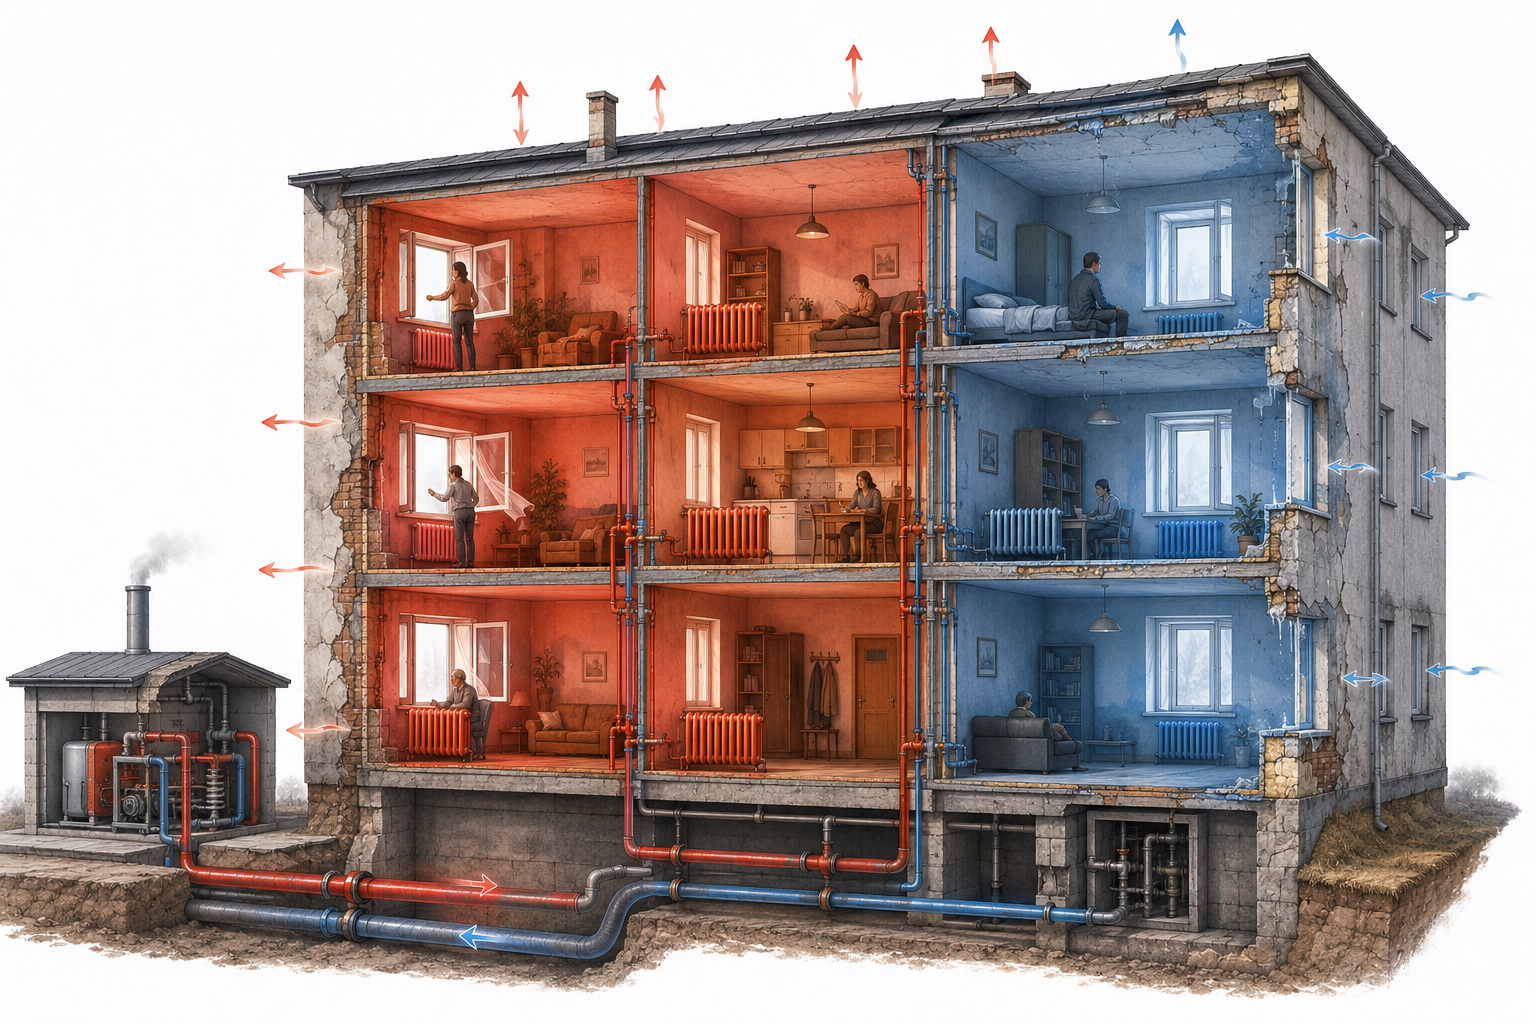
\includegraphics[width=0.75\textwidth,height=0.32\textheight,keepaspectratio]{media/building_heating_imbalance.png}
\caption{老旧建筑供热不均与热损失示意图}
\label{fig:building-heating-imbalance}
\end{figure}

热泵等电气化设备可能抬升冬季电力峰值，围护结构和末端改造又会增加初始投资。方案评价除成本和碳排放外，还需兼顾舒适度、配电容量、居民可负担性、维护条件和极端保供能力。

% 真实照片取自开放获取论文；非本团队拍摄，非本模型实测验证。
% 完整出处、原出版PDF与SHA256见review/photo_sources.json及review/photo_archive。
\subsection{现场对象与负荷参数获取}
围护结构及使用条件影响建筑热损系数与得热。图\ref{fig:real-site-context}引用新疆大学研究人员在乌鲁木齐开展既有建筑改造研究时的建筑和热流计实拍\supcite{33}，说明建筑调查与热工测量对应的现场对象。这组照片作为参数获取的背景资料，原研究建筑与本文算例对象分别处理。

\begin{figure}[htbp]
\centering
\begin{minipage}[t]{0.46\textwidth}
\centering
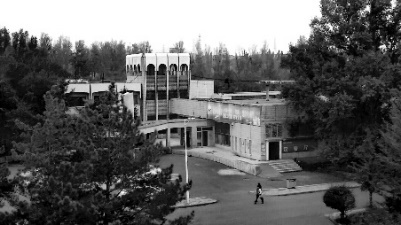
\includegraphics[height=38mm,width=\linewidth,keepaspectratio]{media/site_photos/urumqi_hotel_building.png}
\par\small （a）乌鲁木齐南郊既有旅馆
\end{minipage}\hfill
\begin{minipage}[t]{0.46\textwidth}
\centering
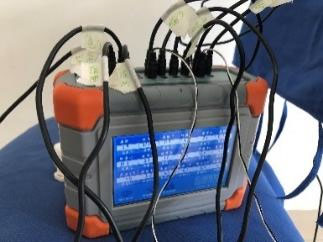
\includegraphics[height=38mm,width=\linewidth,keepaspectratio]{media/site_photos/urumqi_hotel_heat_flux_measurement.jpeg}
\par\small （b）原研究现场使用的多通道热流计
\end{minipage}
\caption{乌鲁木齐既有建筑与热流测量现场。取自Liao等\supcite{33}原图1左、图5左，CC BY 4.0；提取单幅照片并等比例排版，未修改照片内容。}
\label{fig:real-site-context}
\end{figure}


\subsection{传统供热规划的局限}

传统方法多采用“先定技术路线、再核算容量、最后用典型日校核”的流程，难以反映热源、管网、建筑、储热和电网之间的耦合关系。例如，管网降温会影响末端改造，热泵扩容会增加配电投资，储热替代峰值容量还受到充放热功率和时序状态约束。

室外温度、资源可用率、能源价格和设备故障均具有时变性。仅依据年平均负荷或单个设计日规划，难以同时保证全年经济性和寒潮期间的供热可靠性。因此，需要联合确定设备建设、改造、退役与逐时运行方式。

\subsection{国内外研究进展}

\subsubsection{国内研究进展}

国内供热低碳转型主要包括三类路径：既有集中供热系统的热源与管网改造，县城及农村地区的分散清洁供热，以及建筑节能与智慧供热改造。相关实践已覆盖工业余热、大型热泵、低温热网、生物质、太阳能、热计量和气候补偿控制等技术，但各类项目多围绕单项设备或局部系统展开。建筑改造后热源和管网容量如何调整、不同地区集中与分散供热边界如何确定、需求响应能够提供多少稳定调节能力，仍需统一量化。

国内研究已采用综合能源系统优化、多目标规划、鲁棒优化和需求响应等方法。本文重点说明这些方法在最不利房间、二次网失调、回水温度、居民可负担性和极端工况可靠性问题中的适用边界，并统一三个场景的输入与比较口径。

\subsubsection{国外研究进展}

欧洲已形成建筑节能、区域供热、热泵、余热利用和低温热网相结合的技术路径。2024年空间供暖和生活热水约占欧盟家庭终端能源消费的77.1\%\supcite{27}。北欧地区通过地方热力规划确定区域供热与个体供热的服务边界，并将低温输配、余热、大型热泵、可再生能源和季节储热协同配置；第四代区域供热研究进一步强调需求侧柔性与低温热源利用\supcite{20,21}。

国外研究已由单设备优化转向综合规划，常用混合整数规划、多目标优化、随机或鲁棒优化等方法分析热源容量、网络拓扑、储热和建筑柔性。但研究结论受资源、市场和监管条件影响较大，部分模型仍聚焦单一环节，对大规模热泵带来的配电峰值及跨系统约束考虑不足。

余热、热泵、储热与微电网相互影响，研究因而逐步从单项技术评价转向系统配置和联合运行。

\subsubsection{研究不足与本文切入点}

本文重点讨论五项规划问题：系统边界、规划与运行衔接、多目标权衡、物理校核分工和跨场景比较。

第一，系统边界较为分散。热源、管网、建筑、储热和配电系统常由不同模型分别处理，导致热源侧的清洁替代无法同步反映末端适配、回水温度、配电增容和建筑改造需求。热量在总量上平衡，并不意味着温位、空间位置和输配能力同时满足要求。

第二，规划与运行衔接不足。部分研究使用年平均量或少量典型日确定容量，对设备建设、改造和退役的年度时序描述较弱；另一些研究侧重逐时调度，却将容量和网络结构视为已知条件。由此得到的方案可能具有较好的年平均指标，但在寒潮、资源中断或设备故障时缺少可靠容量。

第三，低碳、经济与民生目标缺少统一权衡。年度清洁热占比不能直接代表极寒峰值的化石依赖程度，最低成本方案也未必满足最不利房间温度、居民可负担性和关键建筑保供要求。若不区分生命周期成本、运行现金成本和风险成本，方案之间也难以公平比较。

第四，物理精度与求解规模之间存在矛盾。连续水力、温度衰减、建筑热惯性和设备性能曲线能够提高工程真实性，但全部直接纳入大规模整数模型会显著增加计算难度；过度简化又可能产生温位不匹配、储热状态不闭合或网络输送不可行的方案。本模型据此区分主优化约束与后验校核，并分别说明实际启用范围。

第五，模型的场景迁移能力有限。既有大型热网重构、分散供热清洁化和夏热冬冷地区新建系统在资产基础、负荷特征和主导约束上差异明显，分别建模虽能体现局部特点，却难以形成一致的数据接口、指标口径和比较方法。

基于上述不足，本文以“公用模型内核+场景适配器”为总体结构，将资产演化、带温位能量平衡、储热、建筑状态、电力约束、成本碳排和可靠性纳入统一框架，并针对三类场景加载差异化约束。规划模型负责筛选建设、改造、退役和运行组合，寒潮、资源中断、设备故障及价格变化等情景用于压力测试；本次完成节点热平衡、容量、储热和关键断面的数值校核，连续水力与房间级温度作为工程扩展，从而形成可计算、可比较的供热转型决策流程。


\subsection{数学建模的决策支撑}

供热转型需要同时确定设备、网络与运行方式，并考虑建设阶段和工况变化。热源退役、工业余热接入、管网降温、建筑改造、储热配置和配电增容之间相互影响，任何一项决策都不能脱离其他环节单独评价。传统经验和单项仿真能够判断某一设备或既定方案是否可行，但难以在大量候选组合中同时比较建设时序、容量配置、运行方式和极端工况下的可靠性。

数学模型将热量守恒、温位兼容、设备容量、建筑舒适、储热状态、电网接入和可靠性要求转化为统一的变量与约束，并在工程边界满足的条件下比较生命周期成本、碳排放和风险。模型采用统一口径描述热源、管网、建筑和电网之间的关系，用于筛选满足约束的候选路径。

本文采用“优化筛选---压力测试---数值校核”的计算流程。首先检查负荷、气象、设备性能、能源价格和碳排放因子的来源与适用范围；其次核验热量、电力、储热和等效热状态的守恒残差，并在寒潮、余热下降、设备故障和电网受限等情景下重新调度；最后检查最大流量管段、最远换热站和回水异常节点。原始算例采用关键断面复核；本版另补有限稳态管网模式的自动排除与重算记录，见表\ref{tab:minor-evidence}。

模型可用于候选技术组合筛选、热源与储热容量配置、管网改造与降温路径、建筑改造顺序、设备建设和退役时序以及极端工况下的风险识别。数学建模负责规划决策和方案比较，工程专业仍负责资源调查、设备选型、施工图设计、地质勘察、环保与配电审批及现场调试。只有模型约束、压力测试和专业工程校核均通过的方案，才能作为实施依据。


\clearpage
% !TeX root = ../main.tex
% !TeX program = xelatex
% !TeX encoding = UTF-8
\section{负荷预测与协同优化模型}\label{minor:model}

\subsection{基本假设}

为明确模型适用范围，作如下假设：
\begingroup
\setlength{\parskip}{0pt}
\newcommand{\assumptionline}[2]{\par\noindent\hangindent=1.8em\hangafter=1 #1.\hspace{0.5em}#2}
\assumptionline{1}{研究区域由热源节点、管网节点、换热站和典型建筑构成，同类建筑在保持负荷特征的前提下聚合处理；}
\assumptionline{2}{气象、建筑参数、设备性能和能源价格按1~h时间步长输入；历史窗口按北京时间左闭右开取值：乌鲁木齐为2024年10月10日00:00至2025年4月11日00:00，固原为2024年10月15日00:00至2025年4月16日00:00，武汉为2024年11月16日00:00至2025年3月16日00:00，对应4392~h、4392~h和2880~h；}
\assumptionline{3}{热源容量与出力受运行边界约束，启停及爬坡按设备实际配置加载；}
\assumptionline{4}{主模型采用离散温位和固定供回水温差，候选方案确定后再进行连续温度与水力校核；}
\assumptionline{5}{储热设备具有容量、充放功率、效率和自损失约束，严格互斥模式下同一时段不得同时充热和放热；}
\assumptionline{6}{建筑室温满足舒适边界，原始聚合需求响应保持窗口能量守恒；新增RC分支按室温递推计算供热与散热变化；}
\assumptionline{7}{供暖季逐时计算满足热量守恒、储热状态连续和配电容量限制；}
\assumptionline{8}{温度、流量、压力、可靠性和防冻结等工程指标作为方案可行性的判定条件。}
\par
\endgroup
\vspace{-7.5pt}

三城市供暖季负荷持续曲线见图\ref{fig:code-load-duration}。乌鲁木齐、固原和武汉的峰值负荷分别为1317、1246和598~kW，95\%分位负荷分别为996、900和441~kW，平均负荷分别为588、544和237~kW。相应等效满负荷小时数为1962、1919和1140~h，反映了不同气候条件下的负荷水平与持续特征。图中负荷由气象、建筑参数和场景边界计算得到，用于容量配置与逐时调度，不作为现场实测值。

\begin{figure}[H]
\centering
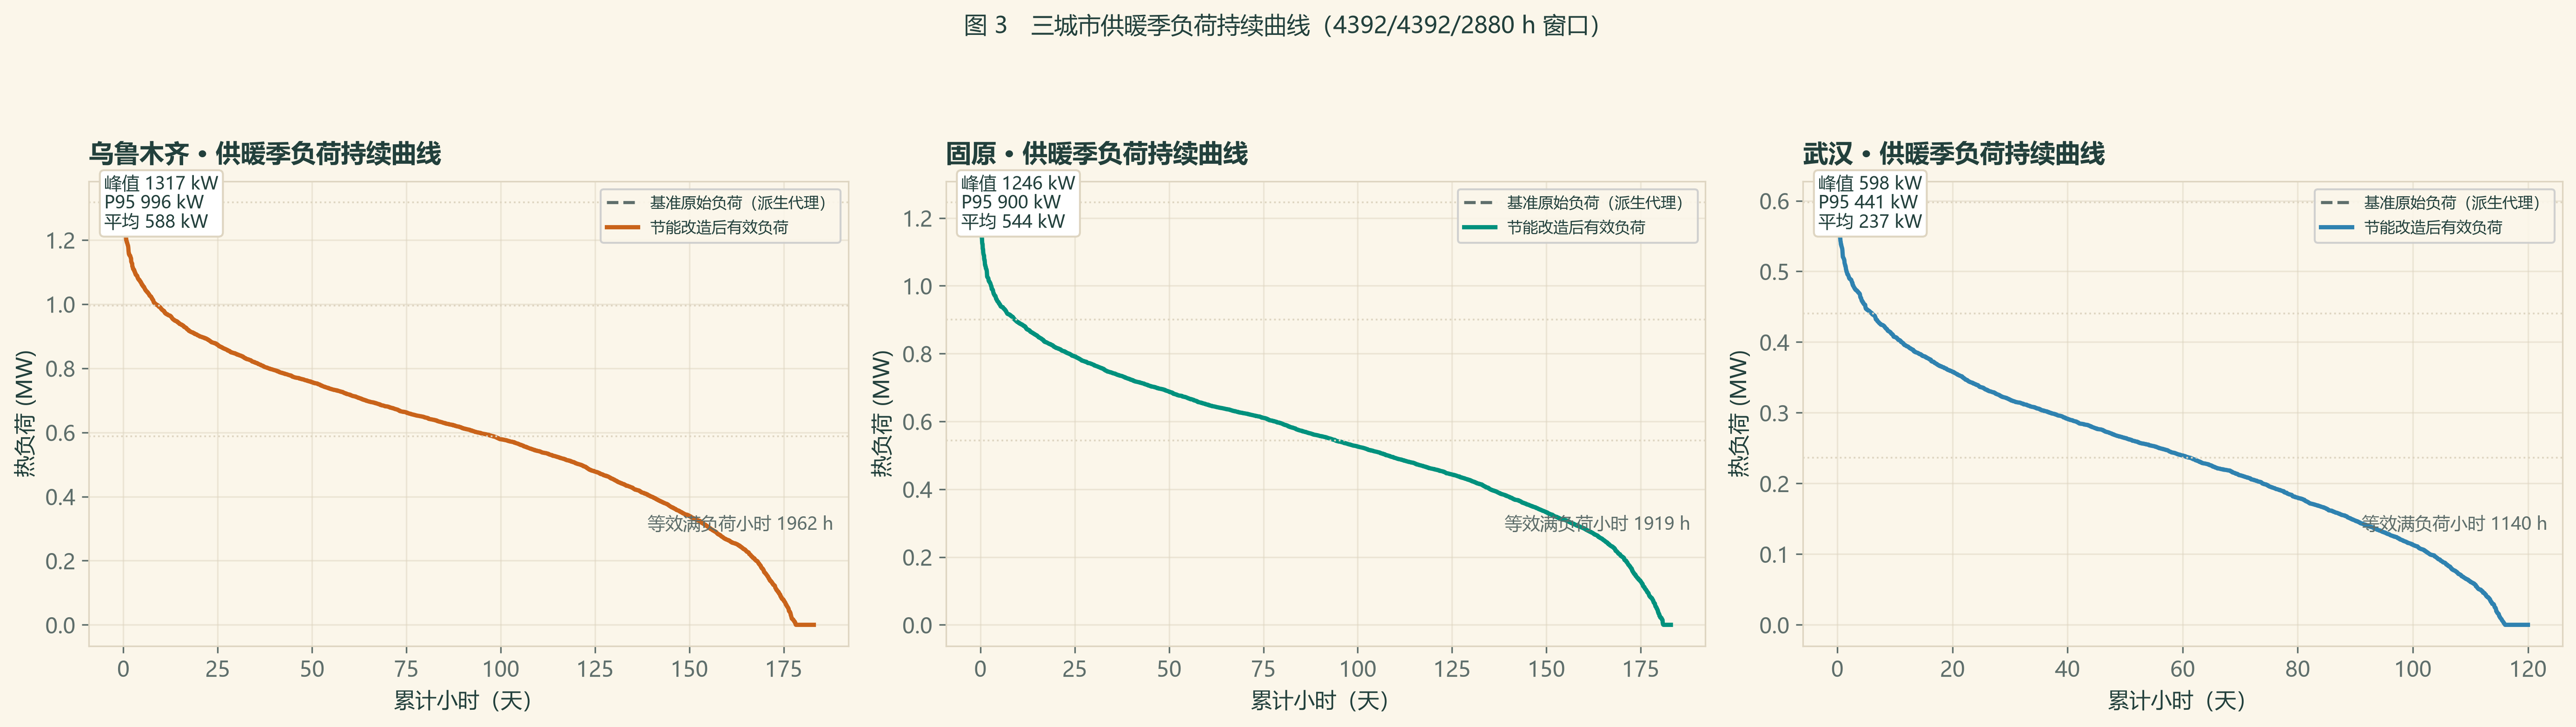
\includegraphics[width=0.98\textwidth,height=0.44\textheight,keepaspectratio,trim=0 0 0 100,clip]{media/code-results/fig03_load_duration_curve.png}
\caption{三城市供暖季负荷持续曲线}
\label{fig:code-load-duration}
\end{figure}

\subsection{模型结构}

模型以建筑逐时负荷为入口，将规划期内的热源建设、设备退役、管网改造、储热配置和配电增容，与供暖季内的热源出力、管网输配、储热充放和建筑热状态统一描述。三个算例均设置3个模型节点，其中2个为聚合需求节点；乌鲁木齐、固原和武汉分别配置7、6、7类热源以及3、2、1条聚合管段。城市层确定资产配置与建设时序，区域层描述热源、管段、换热站和储热之间的能量传输，用户层以聚合节点承载典型建筑负荷与可调节热状态。城市、区域和用户表示决策尺度，不与模型节点逐一对应；算例节点不等同于完整城市地理网络。

公用模型内核包含负荷预测、热源转换、节点平衡、管网输配、储热递推、电力平衡和可靠性约束；场景适配模块根据城市的既有资产、资源条件、网络结构和服务需求加载专用约束。整体关系如图\ref{fig:model-cn-overall}所示。

$n,e,b,k,s$分别表示节点、管段、建筑、热源和储热设备，$g,y,t$为温位、阶段和小时。单阶段算例固定$y$。乌鲁木齐联合求解投资与运行，固原、武汉锚定投资后逐时校核。\textbf{温位、输配、建筑柔性与储热共同约束规划配置。}

\begin{figure}[H]
\centering
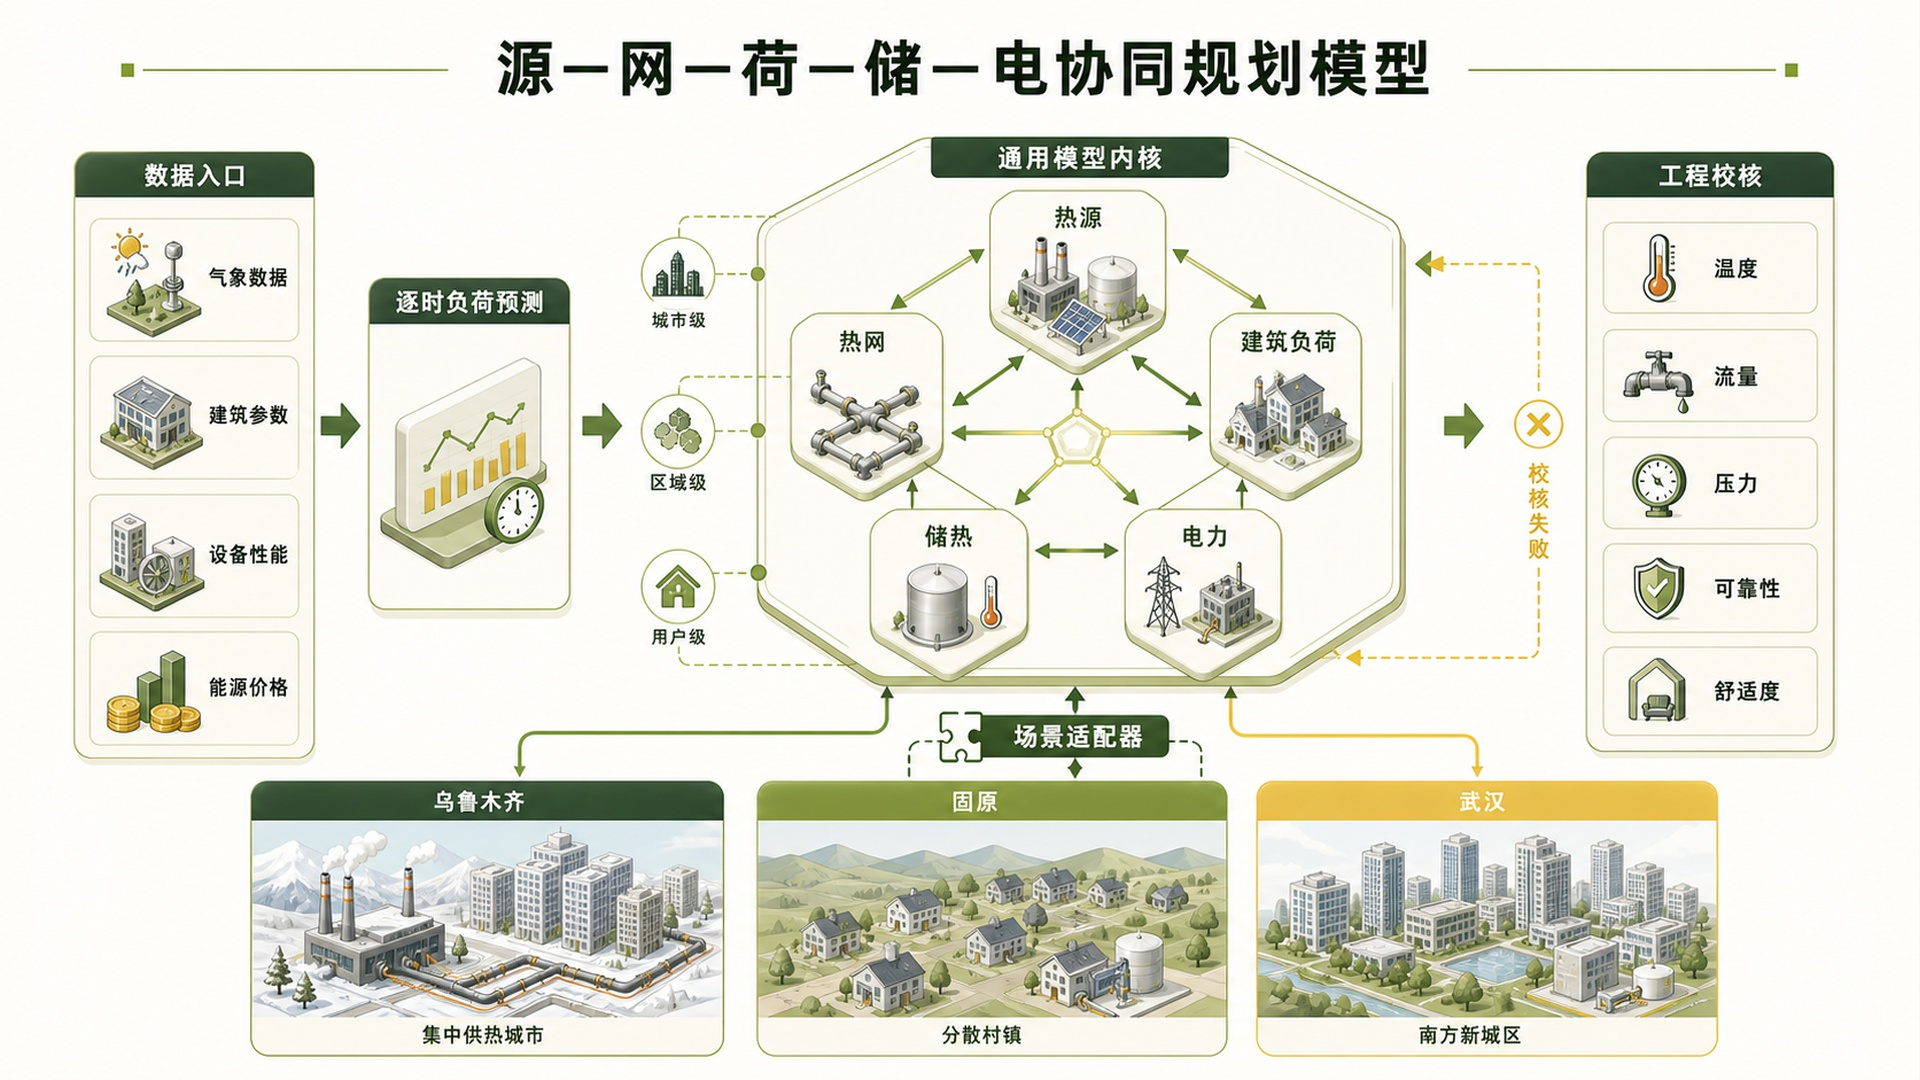
\includegraphics[width=0.76\textwidth,height=0.38\textheight,keepaspectratio]{media/model-cn/01_总体模型框架.jpg}
\caption{协同规划模型框架}
\label{fig:model-cn-overall}
\end{figure}

规划、运行和工程校核采用分层衔接方式。规划层确定建设与容量方案，运行层完成逐时调度；本次数值校核包括热平衡、容量、储热状态、配电边界和失供量检查，工程复核包括温位、关键管段和回水边界。原始算例以事后校核为主；新增有限模式反馈验证另列于表\ref{tab:minor-evidence}。计算流程如图\ref{fig:model-cn-loop}所示。

\begin{figure}[H]
\centering
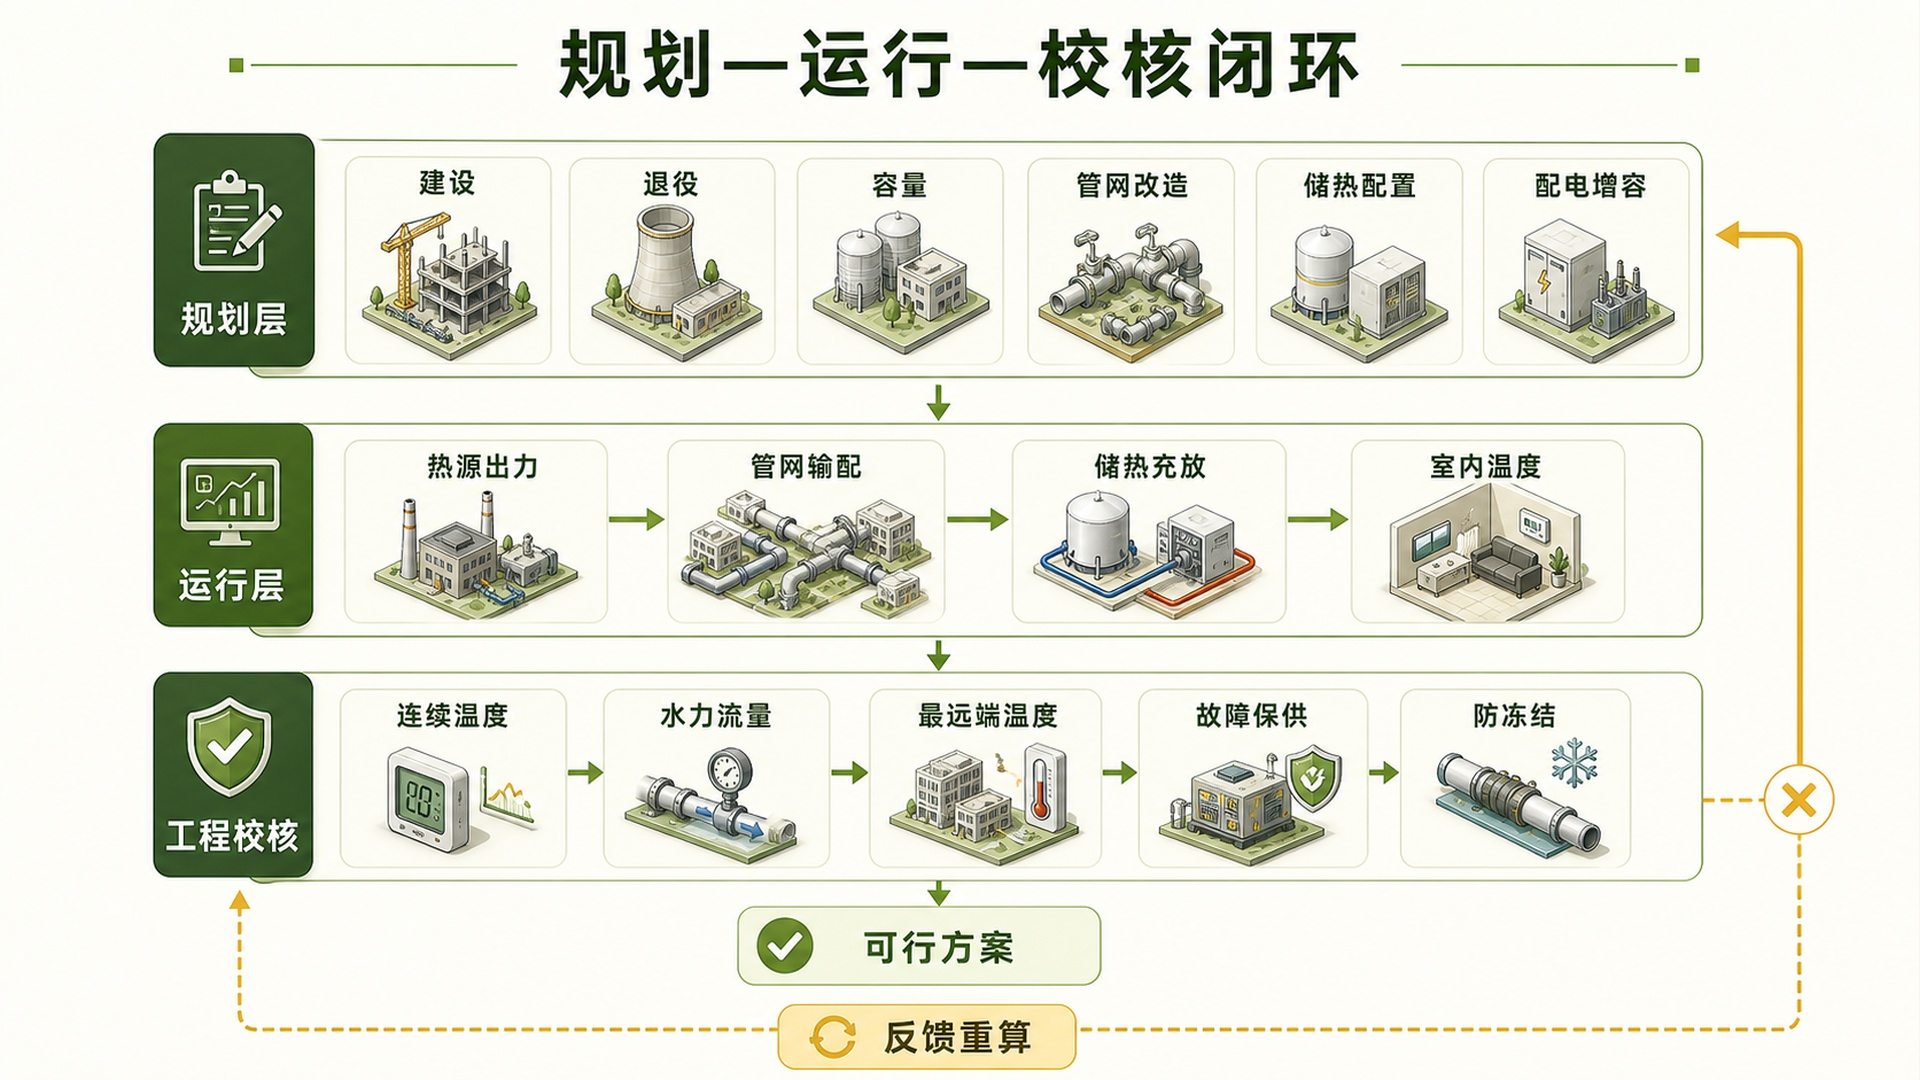
\includegraphics[width=0.76\textwidth,height=0.36\textheight,keepaspectratio]{media/model-cn/05_规划运行校核闭环.jpg}
\caption{规划与校核流程}
\label{fig:model-cn-loop}
\end{figure}

\subsection{建筑负荷}

\subsubsection{负荷分解}

建筑供热负荷由围护结构传热、渗透换气和机械新风热损失构成，同时扣除太阳辐射及人员、设备等内部得热：
\begin{equation}
Q_{b,t}^{\mathrm{load}}=Q_{b,t}^{\mathrm{trans}}+Q_{b,t}^{\mathrm{inf}}+Q_{b,t}^{\mathrm{vent}}-Q_{b,t}^{\mathrm{sol}}-Q_{b,t}^{\mathrm{int}}.
\label{eq:load-decomp}
\end{equation}
围护结构传热与渗透换气损失分别为
\begin{align}
Q_{b,t}^{\mathrm{trans}}&=U_bA_b\left(\theta_{b,t}^{a}-T_t^{\mathrm{out}}\right),\\
Q_{b,t}^{\mathrm{inf}}&=\frac{\rho_ac_an_b^{\mathrm{inf}}V_b}{3.6\times10^6}
\left(\theta_{b,t}^{a}-T_t^{\mathrm{out}}\right).
\end{align}
式中，$U_b$为综合传热系数，使用kW/(m$^2$\,$\cdot$\,K)；若原始值为W/(m$^2$\,$\cdot$\,K)，先除以1000。$A_b$为围护结构面积，$n_b^{\mathrm{inf}}$为换气次数（次/h），$V_b$为建筑体积；当$\rho_a$取kg/m$^3$、$c_a$取J/(kg$\cdot$K)时，除以$3600$完成小时换算，再除以$1000$得到kW。负荷分解关系见图\ref{fig:model-cn-load}。

基准负荷取非负值；建筑热工参数分别登记，调节后的供热量进入节点平衡。

\begin{figure}[H]
\centering
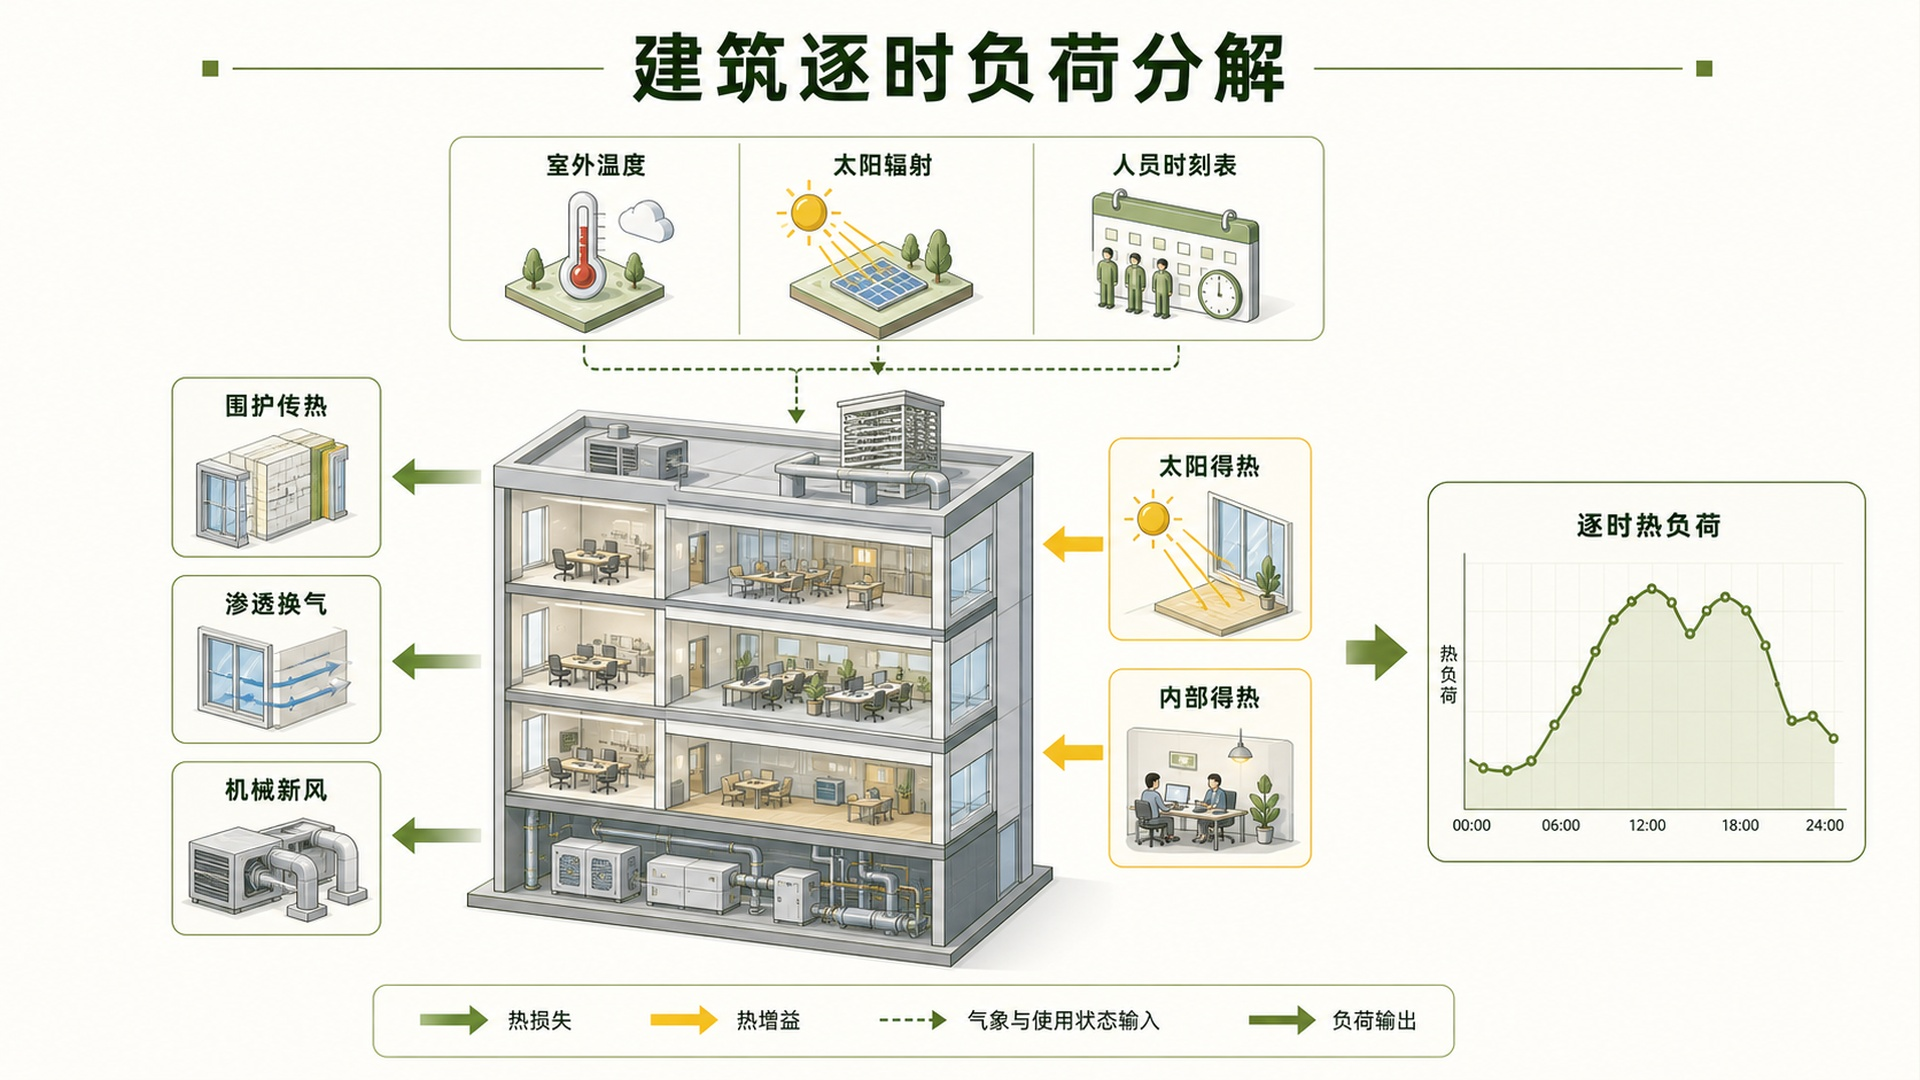
\includegraphics[width=0.76\textwidth,height=0.36\textheight,keepaspectratio]{media/model-cn/02_建筑逐时负荷分解.jpg}
\caption{建筑逐时负荷分解}
\label{fig:model-cn-load}
\end{figure}

\subsubsection{热惯性模型}

原始参数化算例采用单一等效热状态表示用户侧热惯性。令$E_{b,t}$为相对基准状态的蓄热量，$C_b$为聚合节点等效热容，$q_{b,t}^{+}$和$q_{b,t}^{-}$分别表示相对基准的负荷增加量和削减量，$\lambda_b$为每个时间步的衰减率，则
\begin{align}
E_{b,t}&=(1-\lambda_b)E_{b,t-1}+\left(q_{b,t}^{+}-q_{b,t}^{-}\right)\Delta t,\\
\Delta\theta_{b,t}&=\frac{E_{b,t}}{C_b},\qquad \Delta t=1~\mathrm h.
\end{align}
等效温度偏移受上下界约束，需求响应仅在允许窗口内转移负荷，并满足全窗口能量守恒。图\ref{fig:model-cn-2r2c}保留原有双状态概念示意；历史算例采用上述单一等效热状态。新增验证采用下述1R1C递推，分别记录模型版本。

令$D^0_{b,t}$为基准需求，聚合分支的调节量与节点需求通过下式连接：
\begin{align}
Q^{\mathrm h}_{b,t}&=D^0_{b,t}+q^+_{b,t}-q^-_{b,t},&
\underline{\Delta\theta}_b&\le E_{b,t}/C_b\le\overline{\Delta\theta}_b,\\
D_{n,g,t}&=\sum_{b\in\mathcal B_{n,g}}Q^{\mathrm h}_{b,t}+D^{\mathrm{DHW}}_{n,g,t}.
\label{eq:r8m-load-interface}
\end{align}
$\mathcal B_{n,g}$为该节点温位的建筑集合，生活热水按配置计入，建筑供热不重复归集。

\begin{figure}[H]
\centering
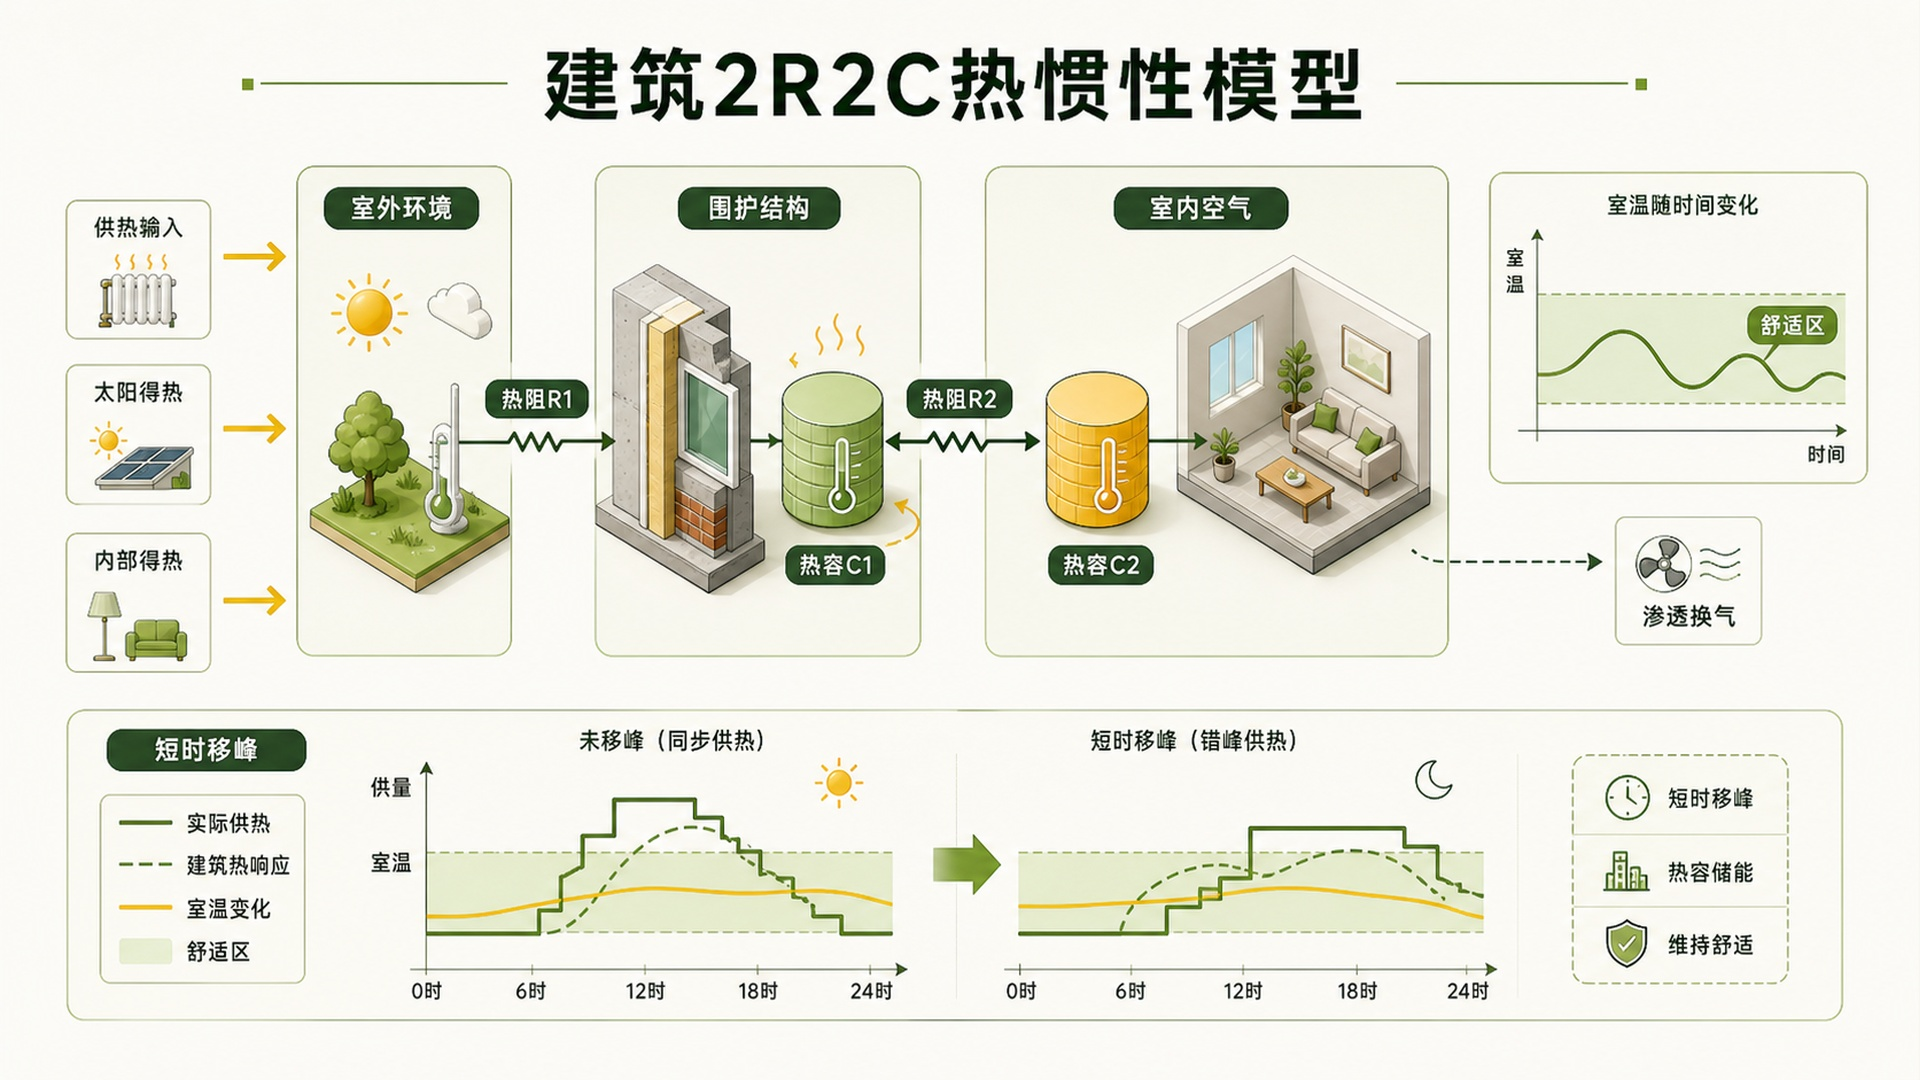
\includegraphics[width=0.76\textwidth,height=0.36\textheight,keepaspectratio]{media/model-cn/03_建筑2R2C热惯性.jpg}
\caption{建筑热惯性概念结构（原框架示意）}
\label{fig:model-cn-2r2c}
\end{figure}


\noindent\textbf{热状态实现的补充。}新增逐楼验证采用1R1C模型\supcite{28}。令$H_b$为围护与换气总热损失系数（kW/K），$C_b$为有效热容（kWh/K），$G_{b,t}$为太阳和内部得热，则在每小时输入不变时，精确积分得到
\begin{equation*}
\begin{aligned}
a_b&=\exp(-H_b\Delta t/C_b),\qquad \beta_b=(1-a_b)/H_b,\\
\theta_{b,t}&=a_b\theta_{b,t-1}+(1-a_b)T_t^{\mathrm{out}}
+\beta_b(Q_{b,t}^{\mathrm h}-Q_{b,t}^{\mathrm c}+G_{b,t}).
\end{aligned}
\end{equation*}
室温满足逐时舒适边界，供热与供冷受设备能力及所选互斥约束限制。初末室温固定，避免通过消耗末态蓄热降低费用；供热量进入节点平衡，电耗汇入公共配电。该分支保留预热造成的额外散热，相关实验与原聚合需求响应结果分开报告。

$\theta_{b,t}$为小时末室温，满足$\underline\theta_{b,t}\le\theta_{b,t}\le\overline\theta_{b,t}$；两类热状态按算例选用，分别得到建筑供热量后，再按节点与温位求和归集。

\subsection{协同约束}

\subsubsection{容量与出力}

设备在规划阶段的可用容量由既有、新建和退役容量共同决定：
\begin{equation}
K_{k,y}=K_k^{\mathrm{exist}}+\sum_{\tau\leq y}K_{k,\tau}^{\mathrm{new}}-\sum_{\tau\leq y}K_{k,\tau}^{\mathrm{ret}}.
\end{equation}
热源逐时出力满足
\begin{equation}
\underline Q_k u_{k,t}\leq Q_{k,t}\leq \overline Q_k u_{k,t},
\qquad Q_{k,t}\leq a_{k,t}K_{k,y},
\end{equation}
其中$u_{k,t}$为启停状态，$a_{k,t}$为可用率。锅炉和热泵的能量转换关系分别为
\begin{equation}
Q_{k,t}^{\mathrm{boiler}}=\eta_k^{\mathrm{boiler}}F_{k,t}^{\mathrm{fuel}},
\qquad Q_{k,t}^{\mathrm{HP}}=COP_{k,t}P_{k,t}^{\mathrm{HP}}.
\end{equation}

燃料输入按低位热值折为kW；热泵取热量为$Q^{\mathrm{HP}}-P^{\mathrm{HP}}$。热电联产满足$\alpha_k^{\min}Q_{k,t}^{\mathrm{CHP}}\le P_{k,t}^{\mathrm{CHP}}\le\alpha_k^{\max}Q_{k,t}^{\mathrm{CHP}}$，售电单列计价；启停与爬坡按配置加载。

\subsubsection{热量平衡}

对节点$n$、温位$g$和时刻$t$，热源输入、上游来热和储热放热应等于用户负荷、储热充热和下游送热：
\begin{multline}
\sum_k Q_{k,n,g,t}+\sum_{a\in\delta^-(n)}\eta_aF_{a,g,t}+\sum_sQ_{s,n,g,t}^{\mathrm{dis}}\\
=D_{n,g,t}+\sum_sQ_{s,n,g,t}^{\mathrm{ch}}+\sum_{a\in\delta^+(n)}F_{a,g,t}.
\label{eq:node-heat-balance}
\end{multline}
该约束按节点、温位和时段分别建立，避免使用全系统总量平衡掩盖局部输配不足。源、网、荷、储、电之间的关系见图\ref{fig:model-cn-unified}。

各温位出力之和为热源总出力。$a$为有向连接，其$F_a$对应物理管段$e$的$F_e^+$或$F_e^-$。\textbf{各环节在同一小时闭合。}

\begin{figure}[H]
\centering
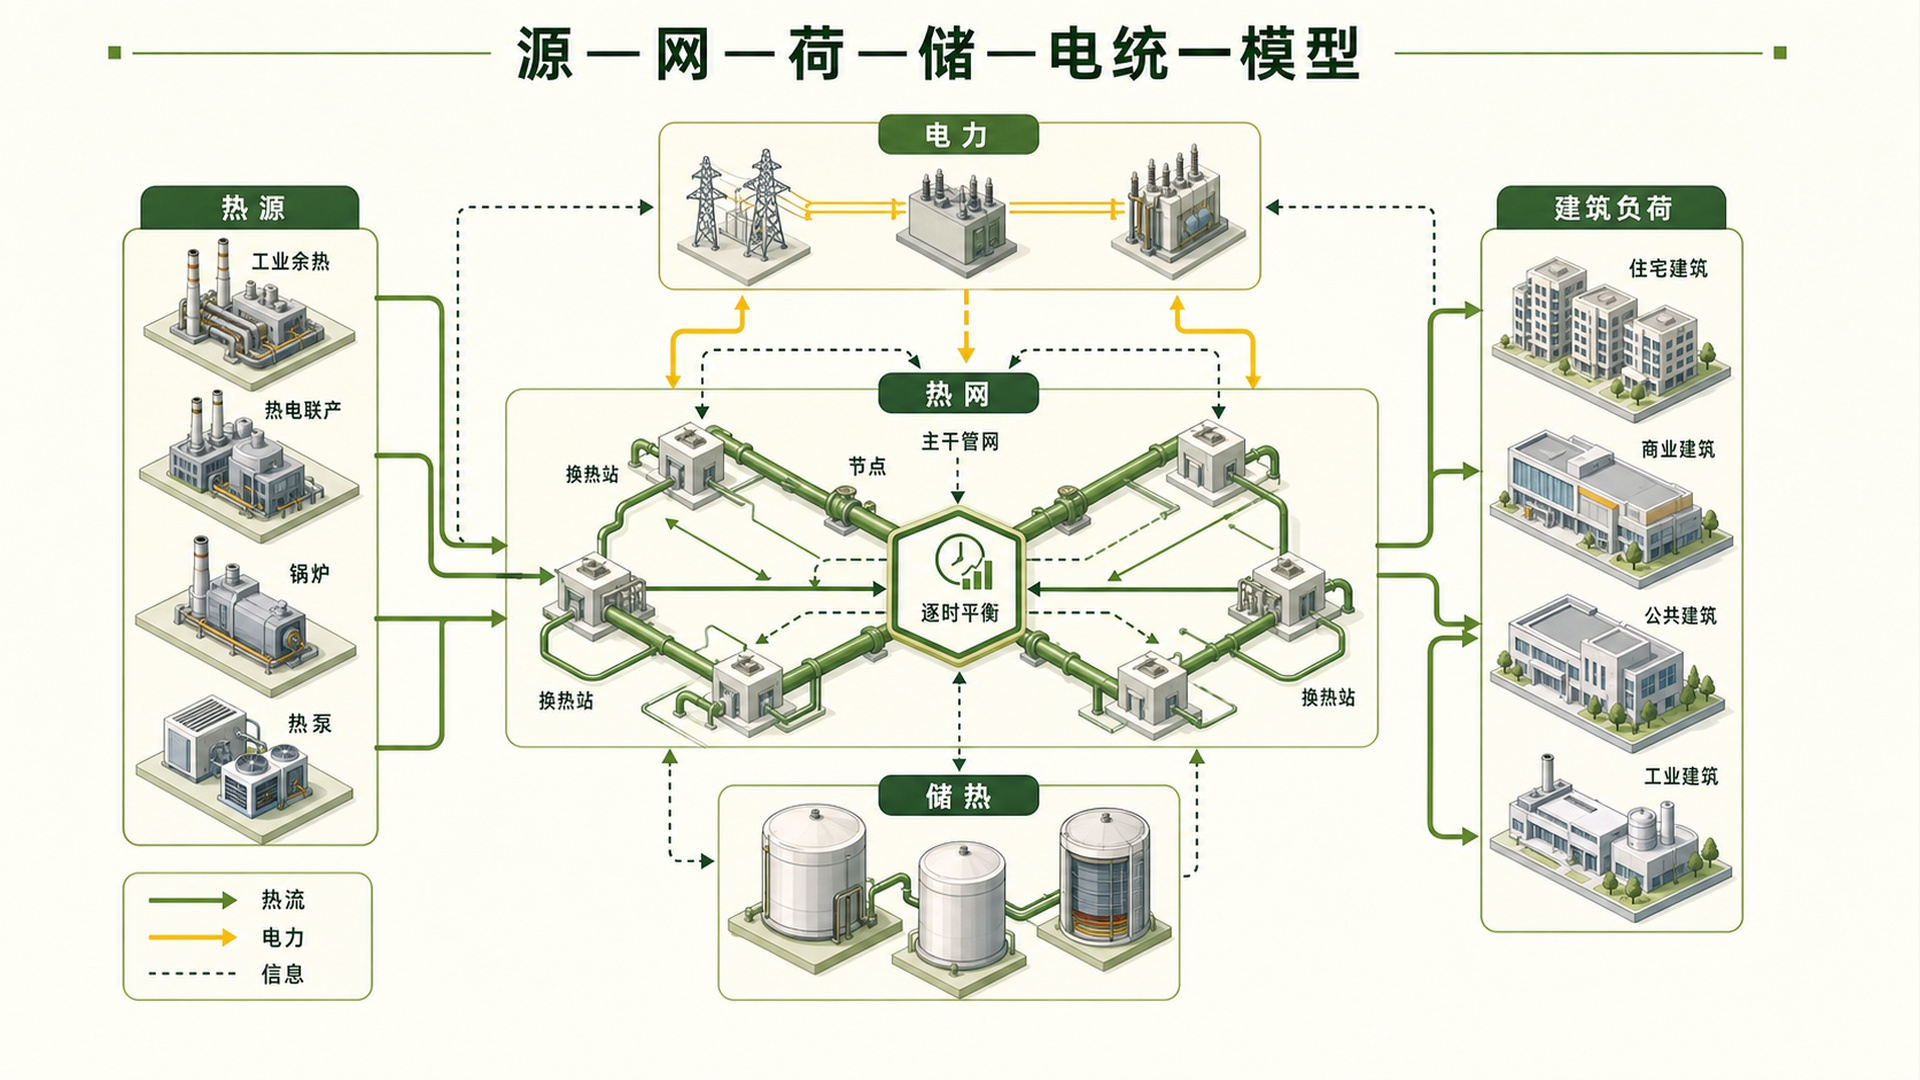
\includegraphics[width=0.76\textwidth,height=0.37\textheight,keepaspectratio]{media/model-cn/04_源网荷储电统一模型.jpg}
\caption{多能流协同关系}
\label{fig:model-cn-unified}
\end{figure}

\subsubsection{温位与管网}

直接供热路径启用时，热源最低供水温度应满足用户温位和换热端差要求：
\begin{equation}
T_k^{\mathrm{src,min}}\geq T_g^{\mathrm{sup}}+\Delta T^{\mathrm{hx}}.
\end{equation}
主模型采用固定温差将热流与质量流量关联：
\begin{equation}
F_{e,g,t}=c_p\Delta T_g\dot m_{e,g,t},
\qquad \sum_g(F^+_{e,g,t}+F^-_{e,g,t})\leq F_e^{\mathrm{exist}}+\sum_d\overline F_{e,d}z_{e,d}.
\end{equation}
温位不匹配的热源不得直接承担高温负荷，需要通过热泵等设备提升温度。梯级利用关系见图\ref{fig:model-cn-grade}。

两方向热流互斥，温级共享管段容量，$\sum_dz_{e,d}\le1$；$c_p$与流量分别采用kJ/(kg$\cdot$K)和kg/s。

\begin{figure}[H]
\centering
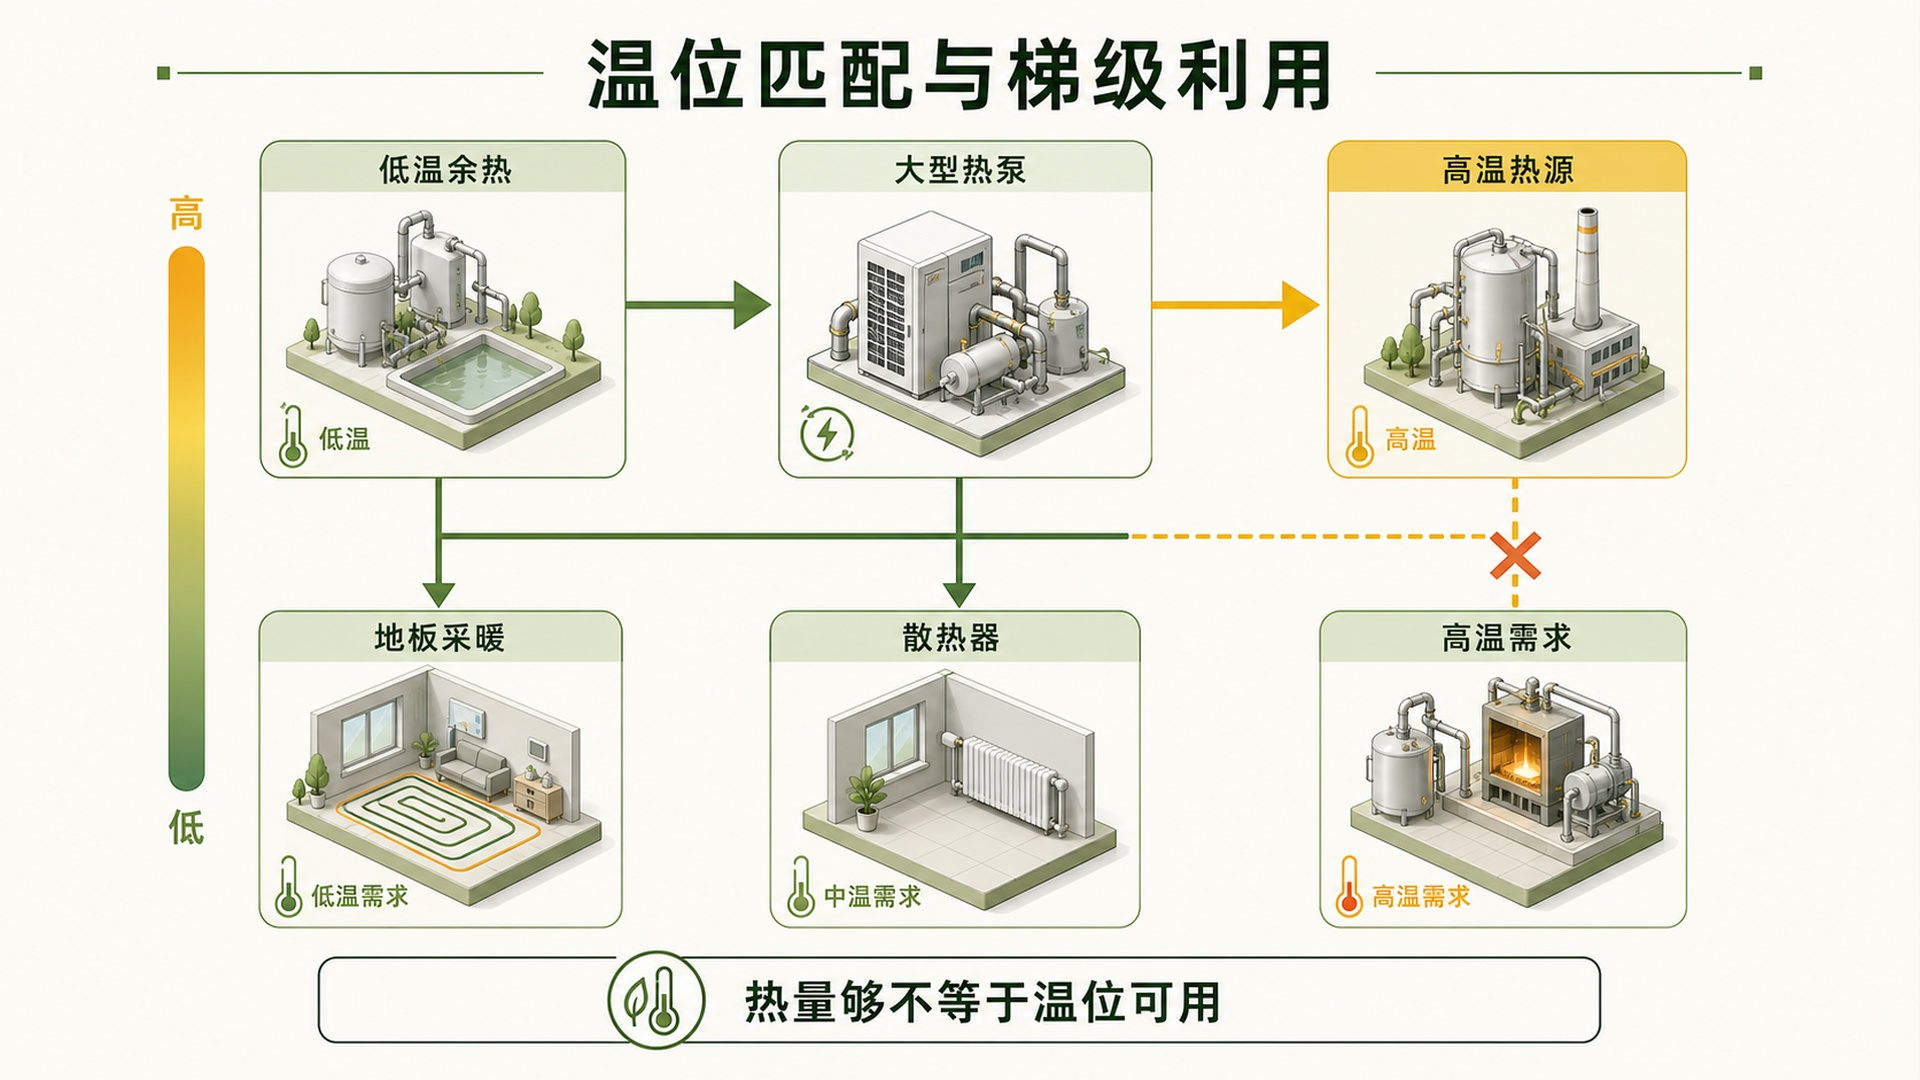
\includegraphics[width=0.76\textwidth,height=0.35\textheight,keepaspectratio]{media/model-cn/06_温位匹配与梯级利用.jpg}
\caption{温位匹配与梯级利用}
\label{fig:model-cn-grade}
\end{figure}

\subsubsection{储热与电力}

储热状态按时段递推：
\begin{equation}
E_{s,t}=(1-\mu_s)E_{s,t-1}+\eta_s^{\mathrm{ch}}Q_{s,t}^{\mathrm{ch}}\Delta t
-\frac{Q_{s,t}^{\mathrm{dis}}\Delta t}{\eta_s^{\mathrm{dis}}}.
\label{eq:storage-state}
\end{equation}

储热容量、充放功率及严格互斥模式的边界为
\begin{align}
0\le E_{s,t}&\le\overline E_s,&
0\le Q^{\mathrm{ch}}_{s,t}&\le\overline Q_s^{\mathrm{ch}},&
0\le Q^{\mathrm{dis}}_{s,t}&\le\overline Q_s^{\mathrm{dis}},\\
Q^{\mathrm{ch}}_{s,t}&\le M_s^{\mathrm{ch}}v_{s,t},&
Q^{\mathrm{dis}}_{s,t}&\le M_s^{\mathrm{dis}}(1-v_{s,t}),&v_{s,t}&\in\{0,1\}.
\end{align}
$\overline E_s$包含既有与新增容量，功率界随配置确定；$M$为候选静态上界。初末边界二选一：
\begin{equation}
\begin{cases}
E_{s,0}=\alpha_s^0\overline E_s,\quad E_{s,T}\ge\alpha_s^{\mathrm{end}}\overline E_s,&\text{固定边界},\\
E_{s,0}=E_{s,T},&\text{循环边界}.
\end{cases}
\end{equation}
能量与功率分别限制储热量和小时调节能力；跨季节应用另需连续覆盖充热季。
热泵、电锅炉、循环泵和储电设备共同进入电力平衡；原聚合算例按系统服务设备汇总：
\begin{multline}
P_t^{\mathrm{imp}}+P_t^{\mathrm{loc}}+P_t^{\mathrm{bat,dis}}\\
=P_t^{\mathrm{base}}+P_t^{\mathrm{HP}}+P_t^{\mathrm{EB}}
+P_t^{\mathrm{pump}}+P_t^{\mathrm{bat,ch}}+P_t^{\mathrm{exp}},\\
0\le P_t^{\mathrm{imp}}\le\overline P^{\mathrm{grid}}.
\end{multline}
储热充放时序与配电峰值的关系见图\ref{fig:model-cn-storage-grid}。

未启用项取零，供冷启用时计入电耗。$P^{\mathrm{loc}}$为公共平衡中的本地电源，独立售电的CHP不抵扣购电；逐楼模型另查楼栋限额。

\begin{figure}[H]
\centering
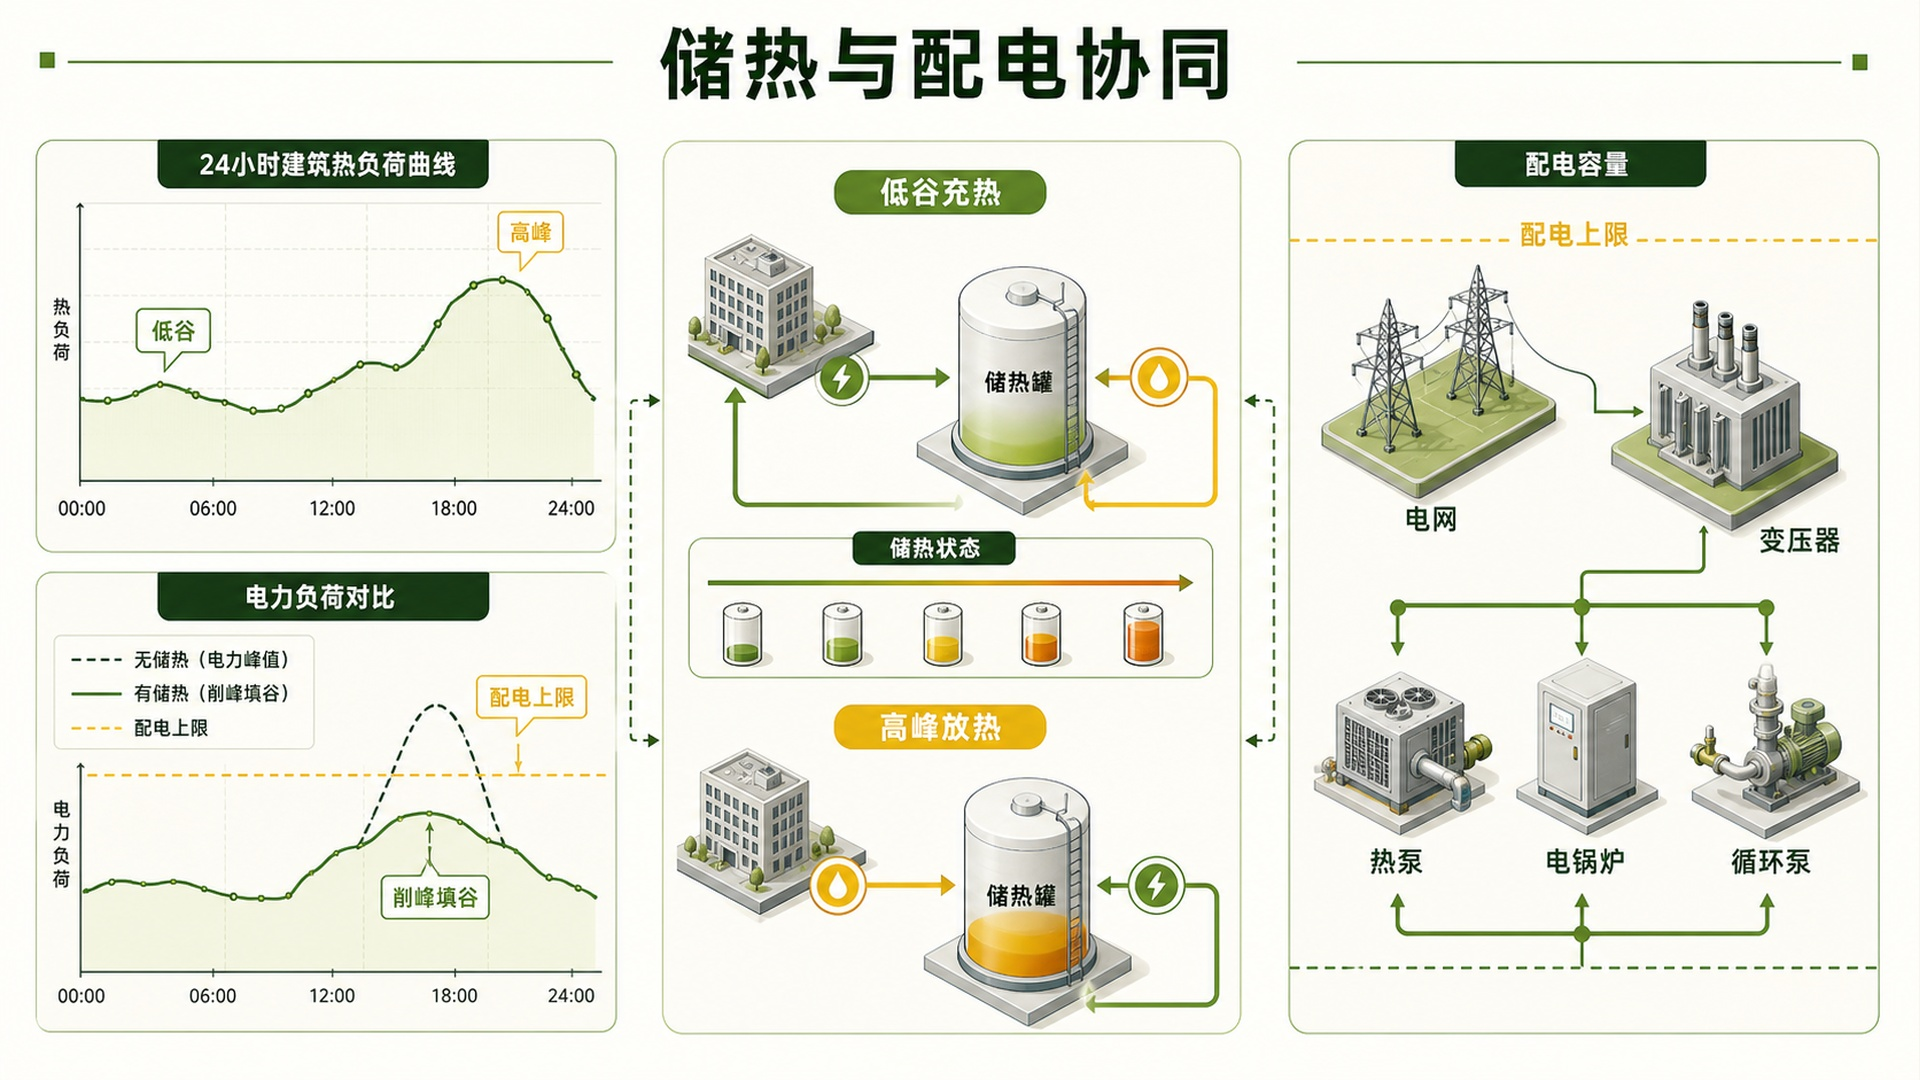
\includegraphics[width=0.76\textwidth,height=0.35\textheight,keepaspectratio]{media/model-cn/07_储热与配电协同.jpg}
\caption{储热与配电协同}
\label{fig:model-cn-storage-grid}
\end{figure}

\subsubsection{目标与可靠性}

模型以生命周期净成本$F^{\mathrm{cost}}$最小为基础目标，并通过$\varepsilon$约束控制碳排放。投资按5\%折现率和20年寿命折算为等年值，目标函数写为
\begin{align}
\min F^{\mathrm{cost}}={}&C^{\mathrm{ann,inv}}+C^{\mathrm{energy}}+C^{\mathrm{carbon}}
+C^{\mathrm{om}}+C^{\mathrm{pen}},\\
C^{\mathrm{ann,inv}}={}&\frac{r(1+r)^{20}}{(1+r)^{20}-1}C^{\mathrm{inv}},
\qquad r=5\%,\\
&F^{\mathrm{CO_2}}\leq\varepsilon_C.
\end{align}
其中$C^{\mathrm{energy}}$为能源费，$C^{\mathrm{carbon}}$为碳费，$C^{\mathrm{om}}$为运维费，$C^{\mathrm{pen}}$为火用失配与舒适偏差惩罚。实际现金成本仅包含发生的能源、运维和碳费用，不与惩罚项混合解释。

碳排放按登记的互不重复核算活动求和：
\begin{equation}
F^{\mathrm{CO_2}}=\sum_{j,t}\gamma_{j,t}A_{j,t}.
\end{equation}
$A$采用已积分活动量：供热与购电为$Q\Delta t$、$P\Delta t$（kWh），到货为本小时质量（kg；速率输入先乘$\Delta t$）。$\gamma$分别为kg~CO$_2$/kWh或kg~CO$_2$/kg。非电热源按供热因子、电驱设备按供电构成计排；启用的供冷与供应链另计，同一能源不重复登记。
失供率定义为
\begin{equation}
U^{\mathrm{un}}=\frac{\sum_tQ_t^{\mathrm{un}}}{\sum_tD_t}\leq\overline U.
\end{equation}
推荐方案取$\overline U=0$。严格平衡主模型中$Q_t^{\mathrm{un}}=0$。用户热状态、设备出力、温位、管网、储热和配电容量均作为硬约束，逐楼分支另执行室温边界，成本与碳排放在可行域内比较。约束关系见图\ref{fig:model-cn-objective}。

\begin{figure}[H]
\centering
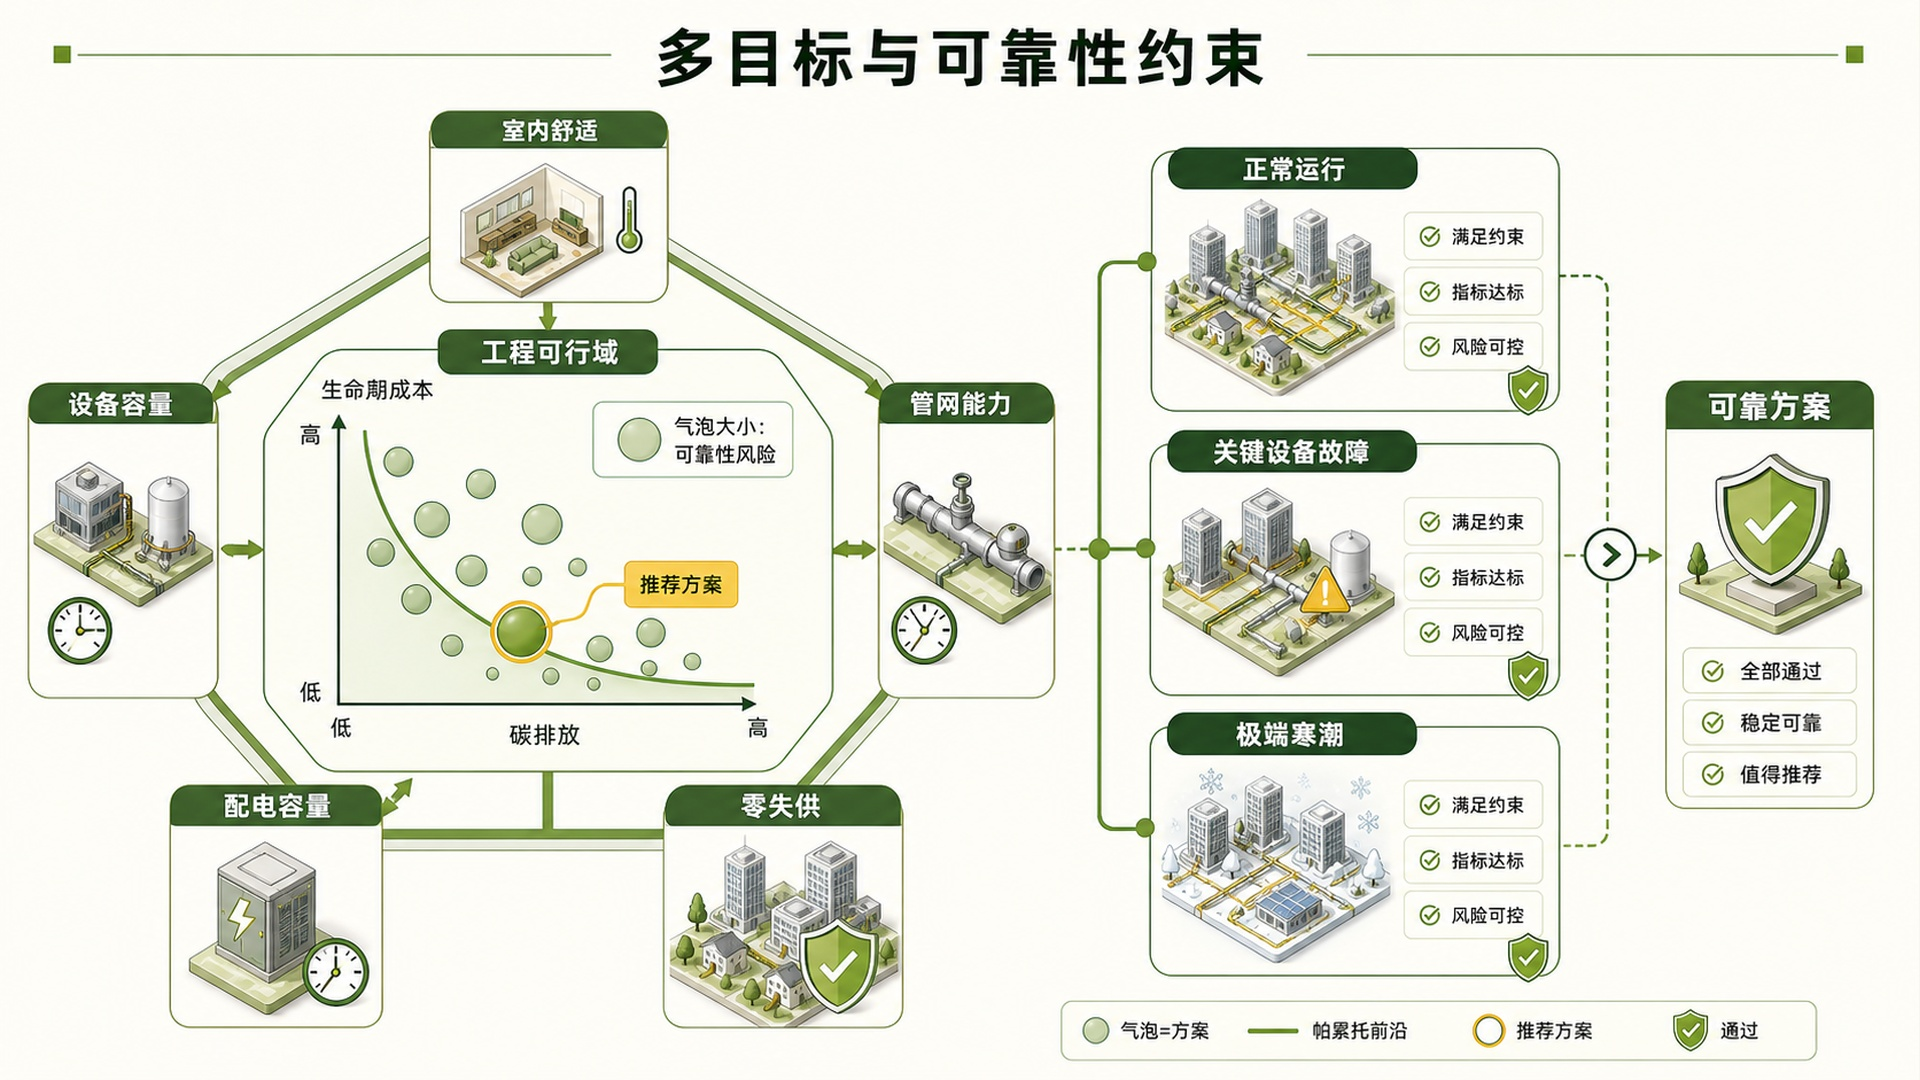
\includegraphics[width=0.76\textwidth,height=0.36\textheight,keepaspectratio]{media/model-cn/08_多目标与可靠性约束.jpg}
\caption{目标函数与可靠性约束}
\label{fig:model-cn-objective}
\end{figure}

\subsection{场景适配}

\subsubsection{乌鲁木齐场景}

乌鲁木齐以既有热电联产、骨干管网和换热站为基础，联合确定燃煤热源退役、工业余热接入、大型热泵、清洁调峰热源、储热及管网降温方案。退役容量必须由清洁热源、储热有效容量和备用容量共同补足：
\begin{equation}
K_{\mathrm{coal},y}^{\mathrm{ret}}\leq K_y^{\mathrm{clean,new}}+K_y^{\mathrm{storage,credit}}+K_y^{\mathrm{reserve}}.
\end{equation}
工业余热满足$0\leq Q_t^{\mathrm{waste}}\leq\overline Q_t^{\mathrm{waste}}$，温位不足时通过热泵升温。模型结构见图\ref{fig:model-cn-urumqi}。

储热有效容量采用满足峰值持续时间及状态边界的放热功率。\textbf{退役受可持续保供能力限制}，压力工况保持容量配置不变。

\begin{figure}[H]
\centering
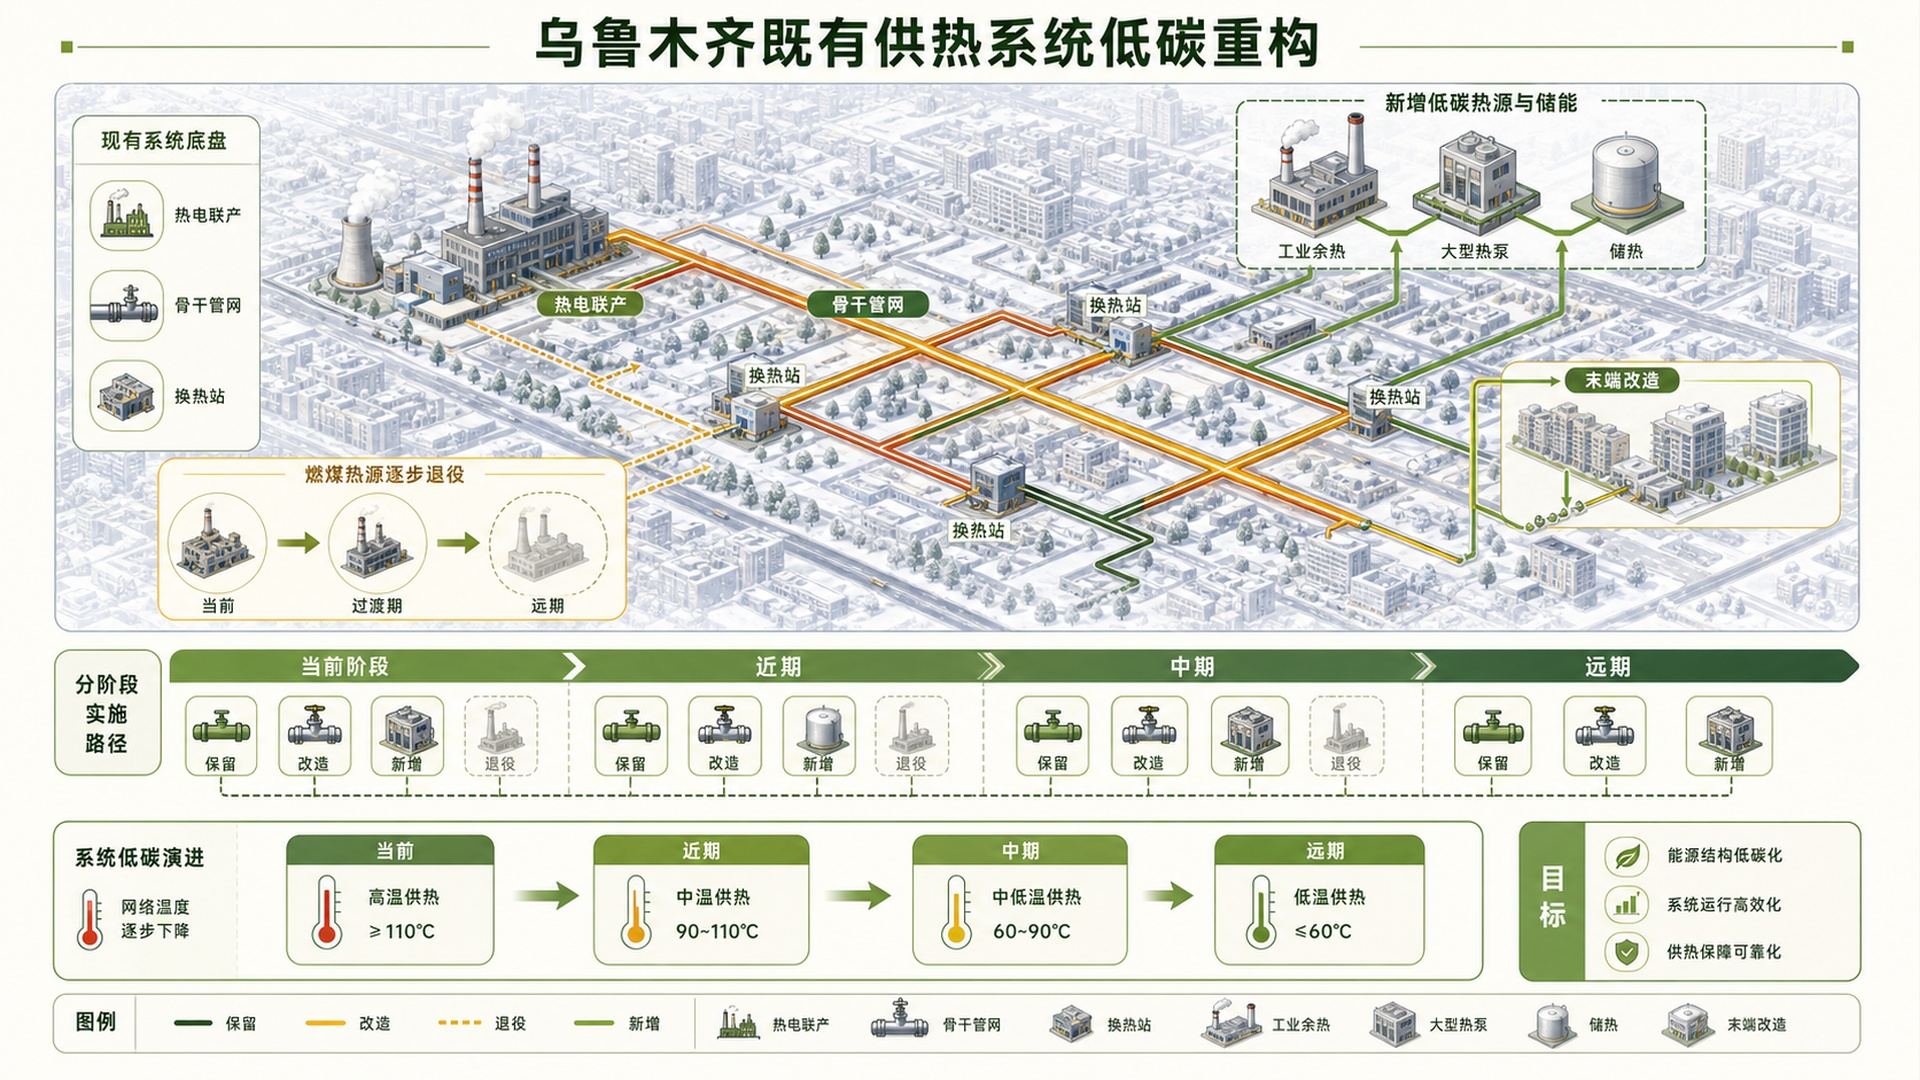
\includegraphics[width=0.77\textwidth,height=0.38\textheight,keepaspectratio]{media/model-cn/09_乌鲁木齐低碳重构.jpg}
\caption{乌鲁木齐低碳重构}
\label{fig:model-cn-urumqi}
\end{figure}

候选方案确定后，校核最远换热站供水温度、关键管段流量、回水温度、供回水温差、热源N-1、寒潮零失供以及管网降温与建筑末端改造的协调关系，见图\ref{fig:model-cn-urumqi-check}。详细约束列于附录1。

\begin{figure}[H]
\centering
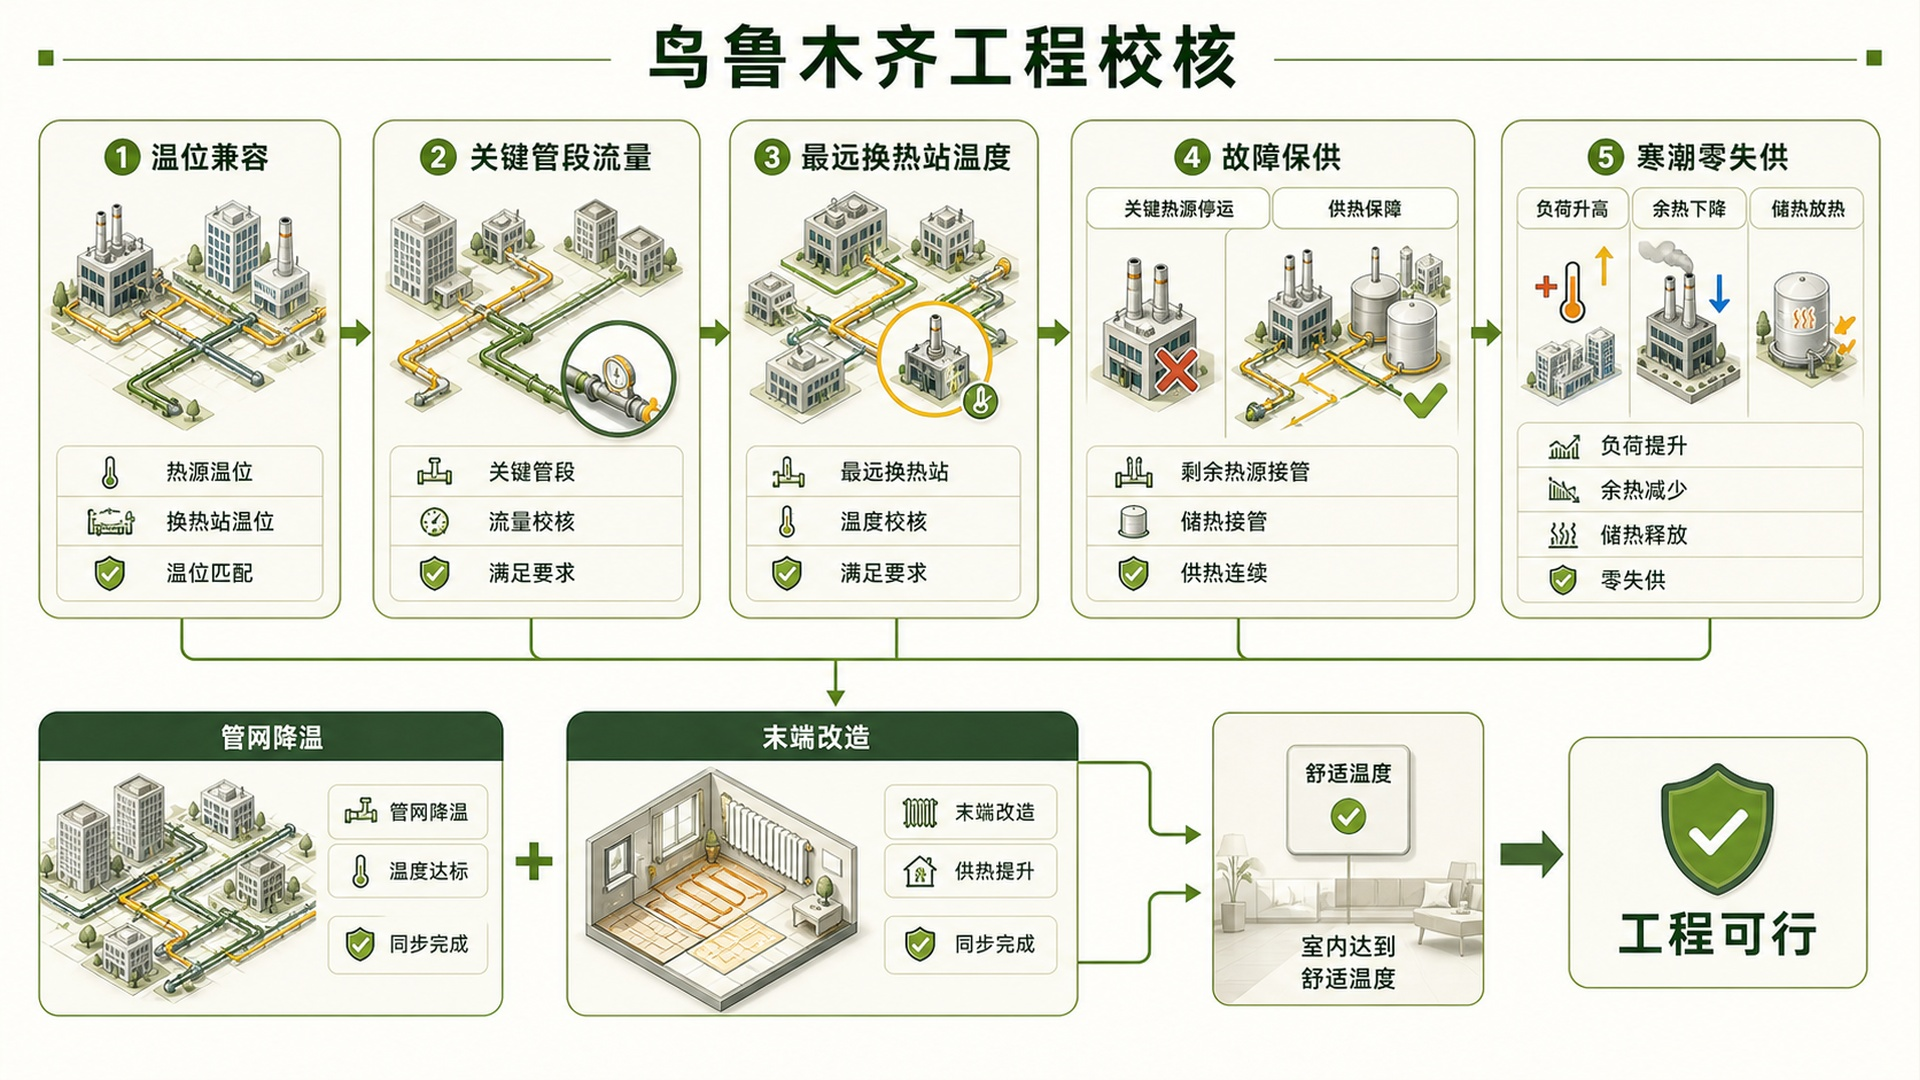
\includegraphics[width=0.76\textwidth,height=0.35\textheight,keepaspectratio]{media/model-cn/10_乌鲁木齐工程校核.jpg}
\caption{乌鲁木齐工程校核}
\label{fig:model-cn-urumqi-check}
\end{figure}

\subsubsection{固原场景}

固原以村镇、片区和区域微网为基本单元。原框架以如下选址和用户分配式定义空间组织接口；已报告算例在给定站点、用户归属及候选连接下求解容量与运行。扩展接口中，用户分配和服务半径满足
\begin{equation}
\sum_i x_{i,b}=1,\qquad x_{i,b}\leq z_i^{\mathrm{site}},\qquad
d_{i,b}x_{i,b}\leq\overline d_i,
\end{equation}
热源容量满足$\sum_bD_b^{\mathrm{peak}}x_{i,b}\leq K_i$。空间组织和技术配置见图\ref{fig:model-cn-guyuan}。

\begin{figure}[H]
\centering
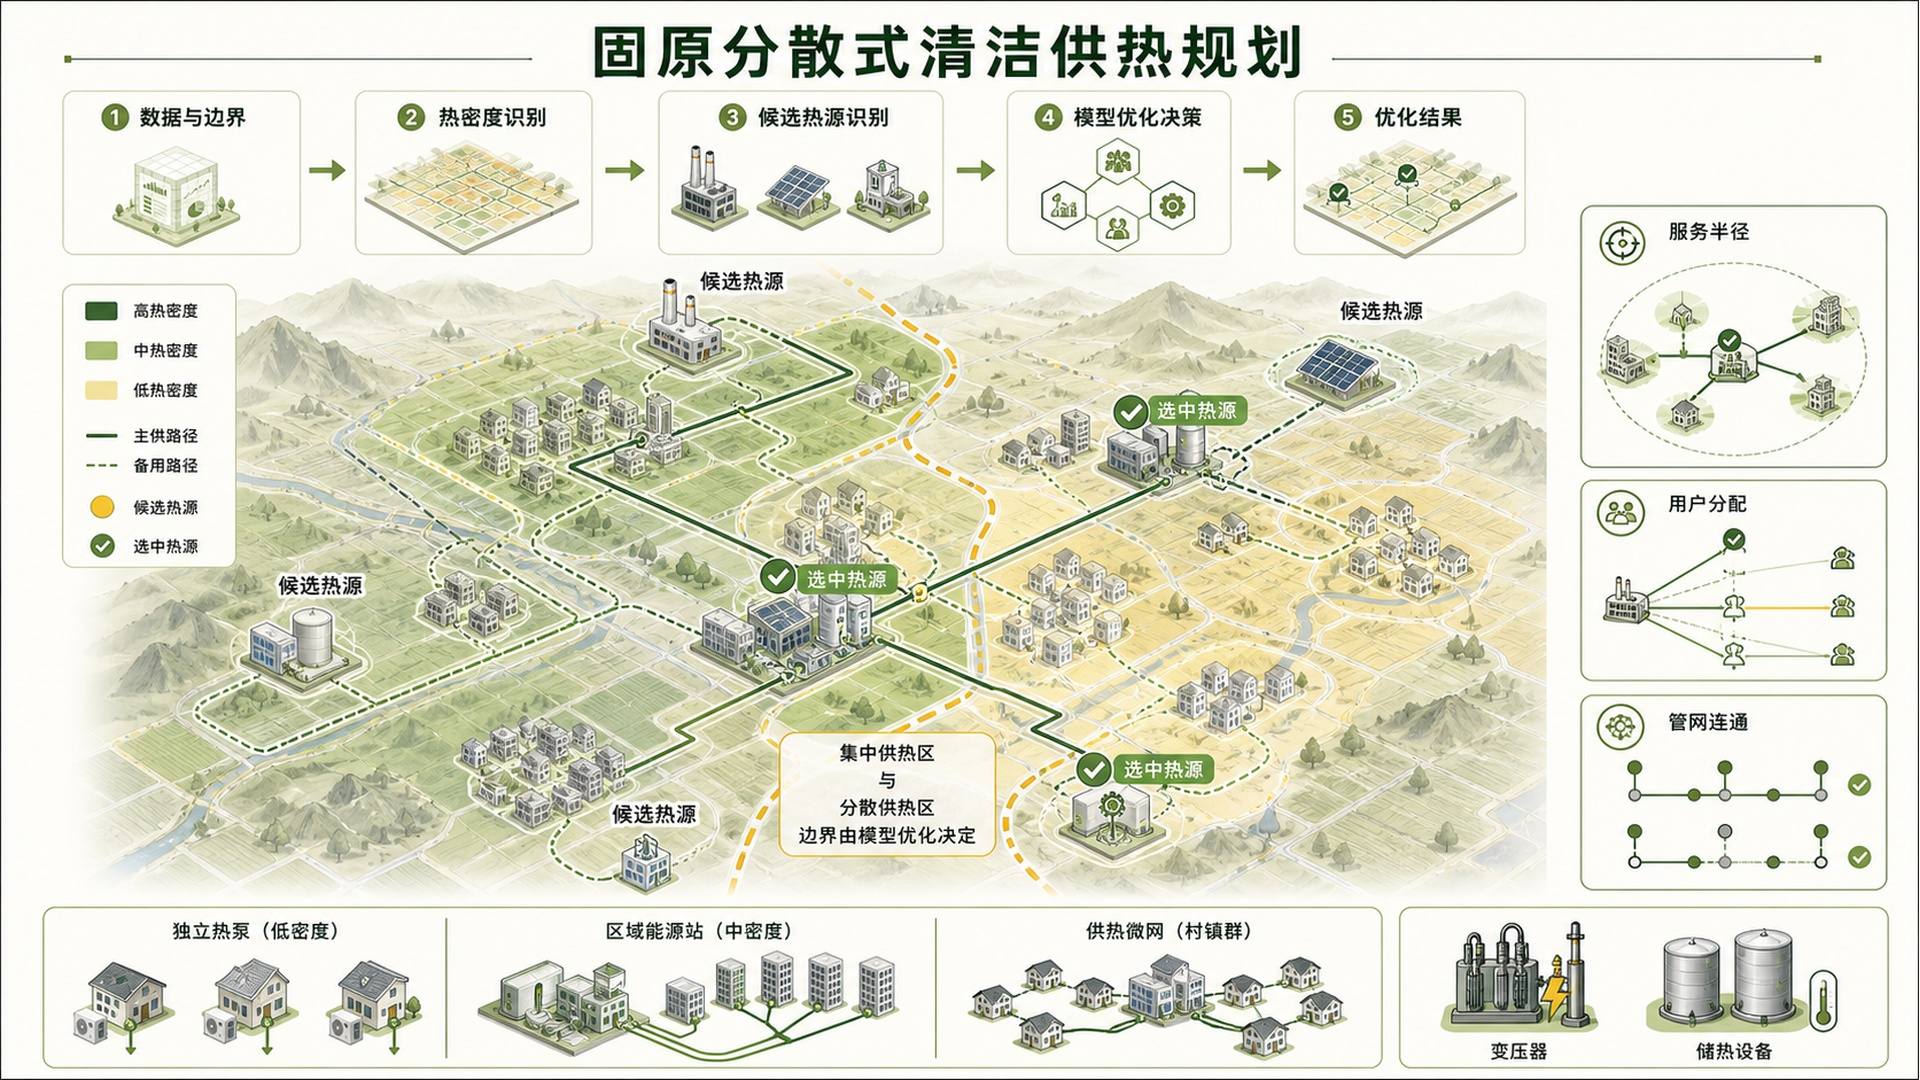
\includegraphics[width=0.77\textwidth,height=0.38\textheight,keepaspectratio]{media/model-cn/11_固原分散供热规划.jpg}
\caption{固原分散供热规划}
\label{fig:model-cn-guyuan}
\end{figure}

生物质燃料按到货、库存和消耗逐时递推，并在电网或单一热源故障下检查关键用户保供。燃料供应与孤岛运行关系见图\ref{fig:model-cn-guyuan-risk}，详细约束列于附录1。

\begin{figure}[H]
\centering
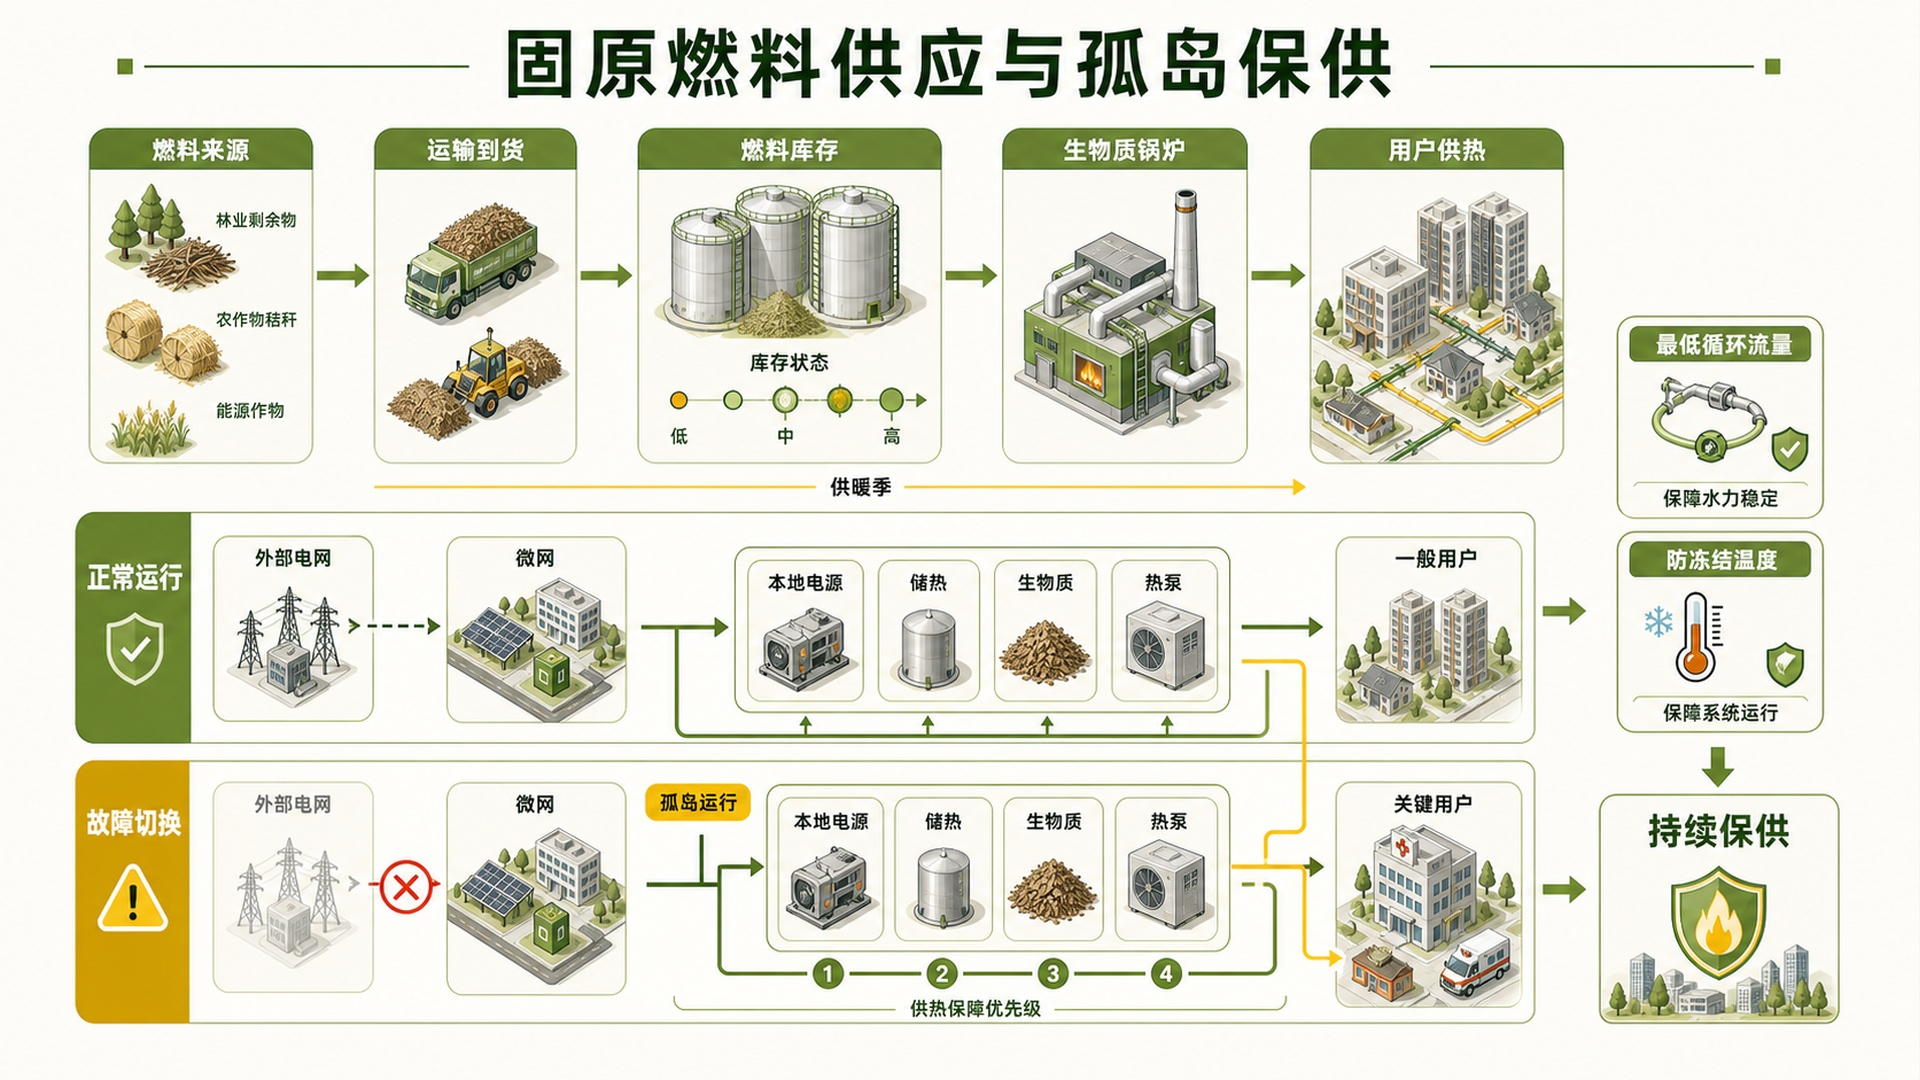
\includegraphics[width=0.76\textwidth,height=0.35\textheight,keepaspectratio]{media/model-cn/12_固原燃料与孤岛保供.jpg}
\caption{固原燃料与孤岛保供}
\label{fig:model-cn-guyuan-risk}
\end{figure}

\subsubsection{武汉场景}

武汉以楼栋和小区为主要空间单元。原框架用下式表达独立楼宇、区域能源站、低温热网和第五代区域供热供冷系统的形态选择接口；已报告算例按给定形态装配设备与运行约束：
\begin{equation}
z_i^{\mathrm{building}}+z_i^{\mathrm{station}}+z_i^{\mathrm{LTN}}+z_i^{\mathrm{5GDHC}}=1.
\end{equation}
四类形态的适用边界见图\ref{fig:model-cn-wuhan-types}。

\begin{figure}[H]
\centering
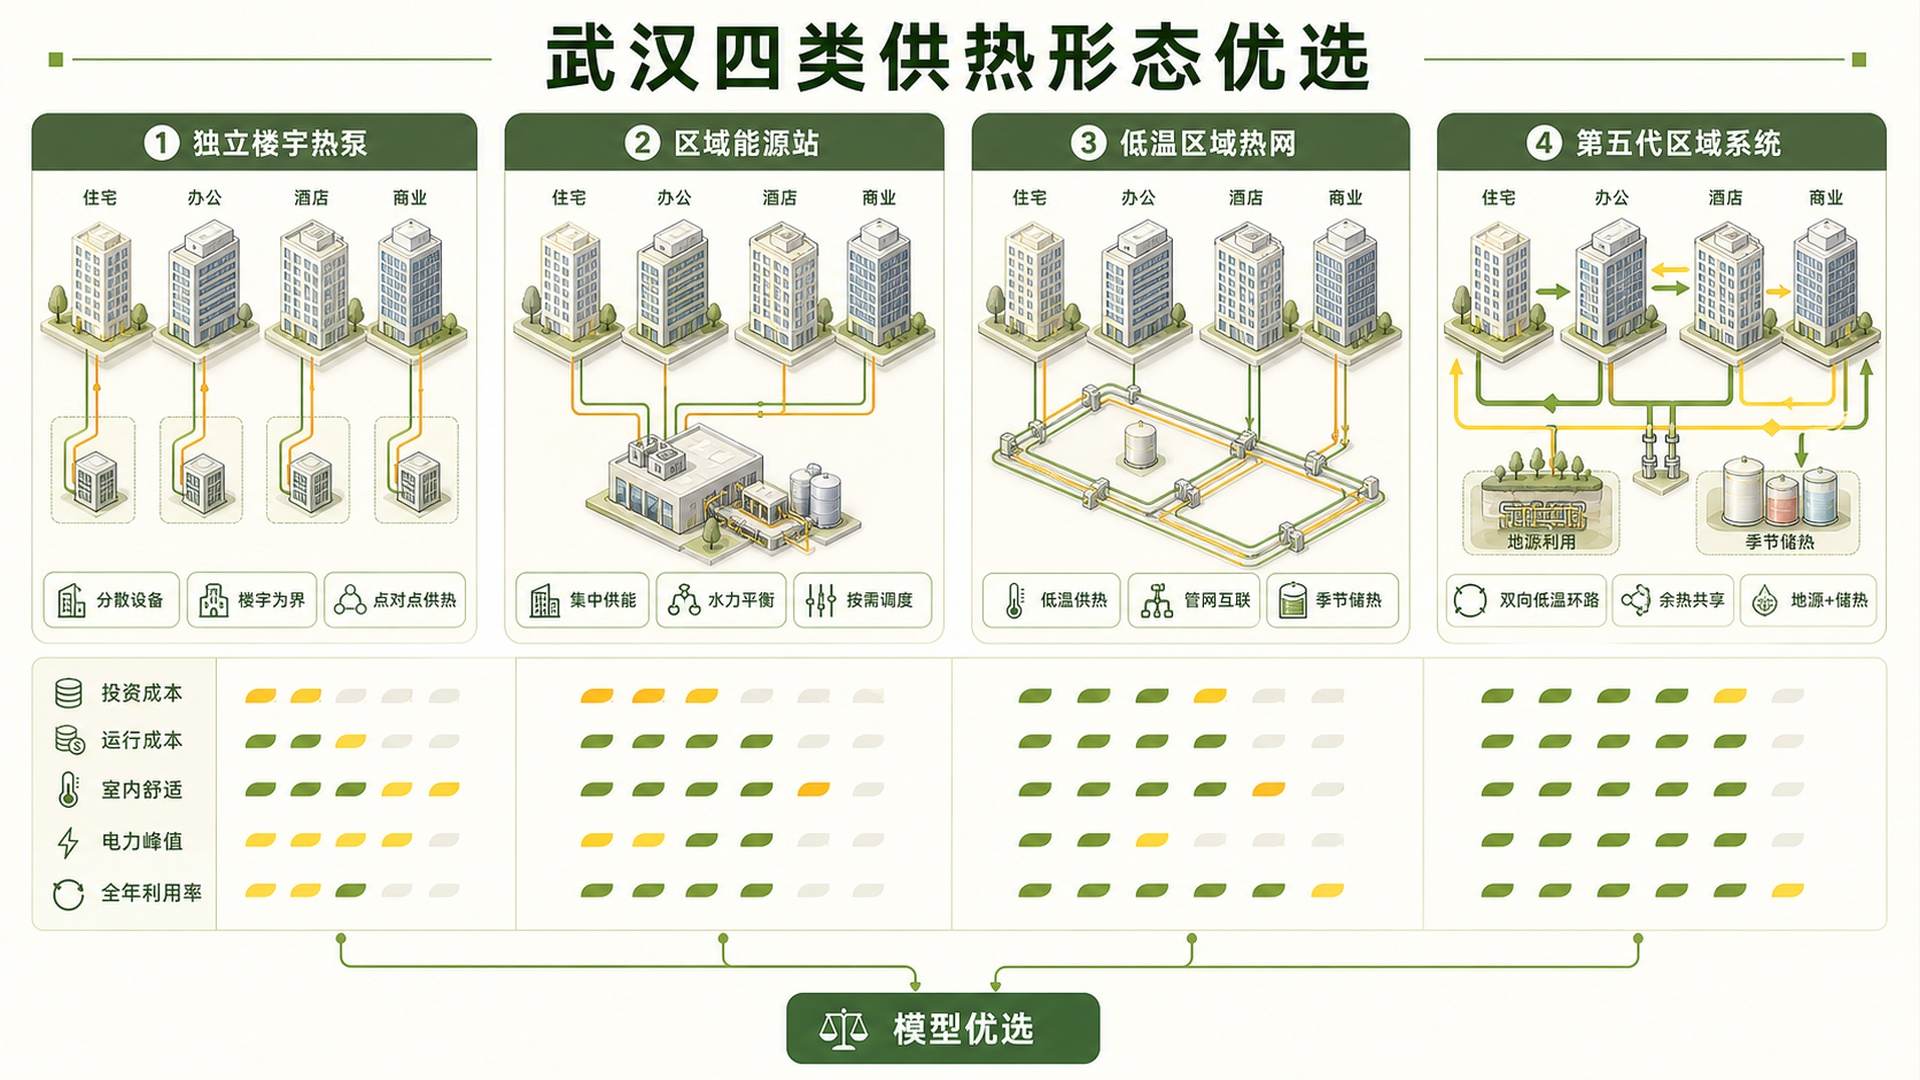
\includegraphics[width=0.76\textwidth,height=0.35\textheight,keepaspectratio]{media/model-cn/13_武汉四类供热形态.jpg}
\caption{武汉供热形态}
\label{fig:model-cn-wuhan-types}
\end{figure}

武汉场景重点考虑供热、间歇预热和楼栋配电容量，供冷与生活热水按配置启用；温湿度、新风、结露、除霜、地源年度平衡与噪声保留为扩展约束。其中，启用结露检查时，低温末端表面温度应高于露点并保留安全裕度：
\begin{equation}
T_{b,t}^{\mathrm{surface}}\geq T_{b,t}^{\mathrm{dew}}+\Delta T^{\mathrm{safe}}.
\end{equation}
主要约束见图\ref{fig:model-cn-wuhan-quality}，详细表达列于附录1。

逐楼舒适边界按占用时段配置，预热受热容、散热、设备与配电共同限制；恢复室温由状态递推获得。

\begin{figure}[H]
\centering
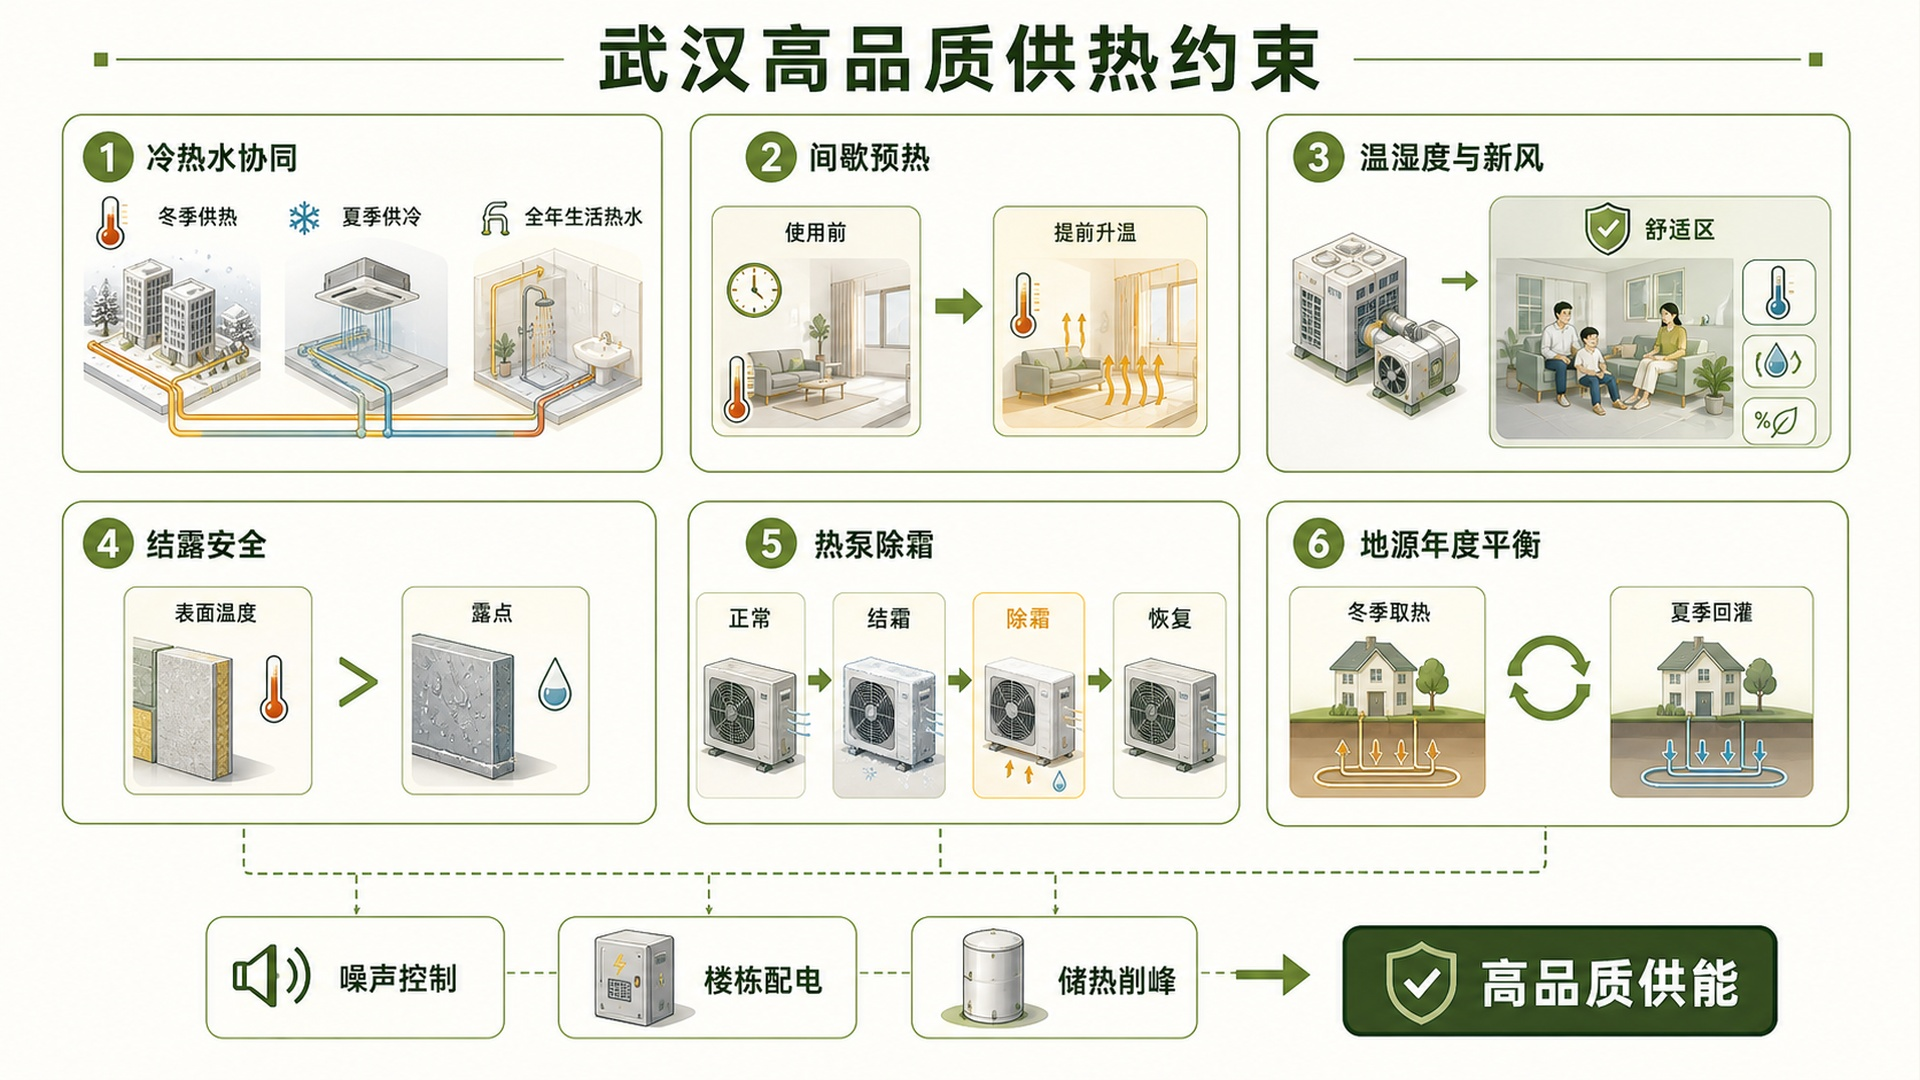
\includegraphics[width=0.76\textwidth,height=0.35\textheight,keepaspectratio]{media/model-cn/14_武汉高品质供热约束.jpg}
\caption{武汉供热约束}
\label{fig:model-cn-wuhan-quality}
\end{figure}

\subsection{场景差异}

三类场景共享负荷预测、能量平衡、容量演化、储热递推和舒适度约束，但规划对象和主导边界不同。乌鲁木齐侧重存量资产重构与极寒保供，固原侧重空间选址、燃料供应和微网可靠性，武汉侧重系统形态与多服务品质。共核与差异关系见图\ref{fig:model-cn-adapters}。

表中包含扩展边界，实际启用项见配置矩阵；同城按相同服务范围比较，跨城统一单位指标。

\begin{figure}[H]
\centering
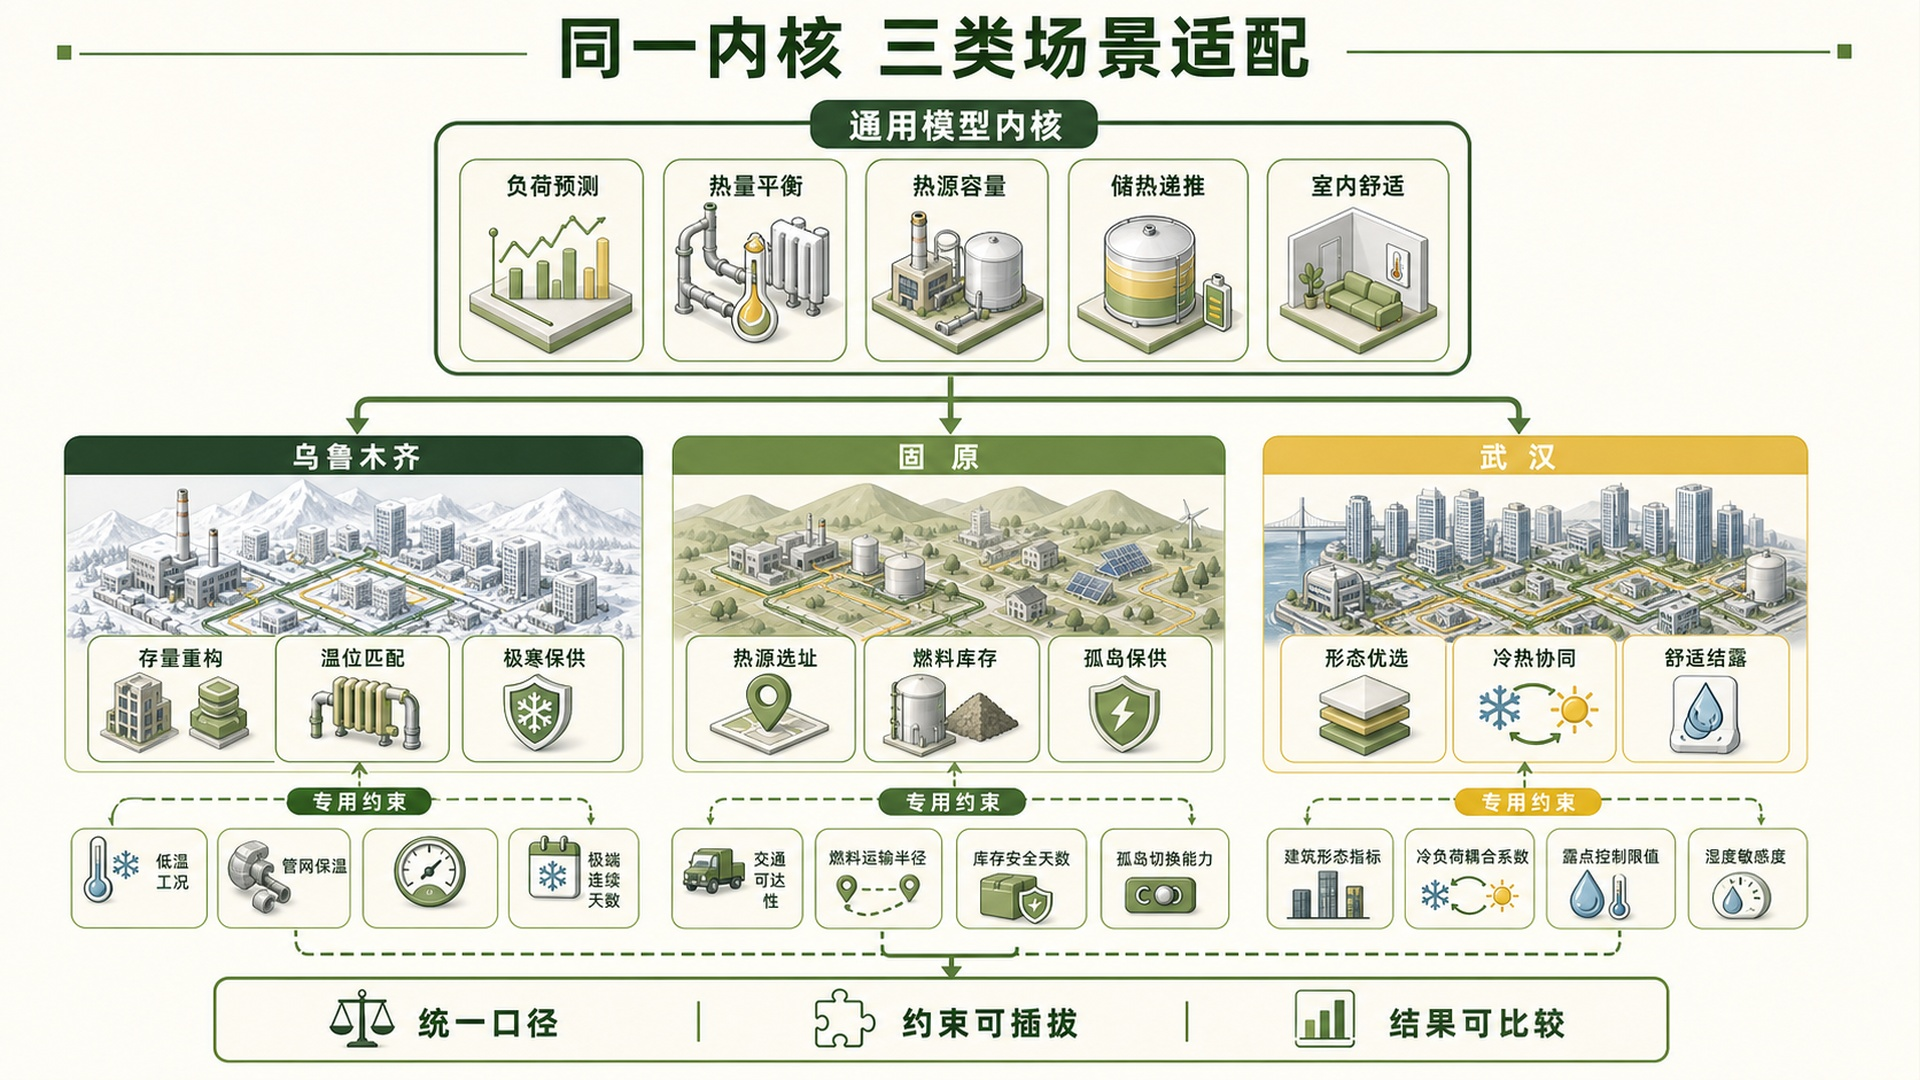
\includegraphics[width=0.76\textwidth,height=0.36\textheight,keepaspectratio]{media/model-cn/15_三城市共核异构.jpg}
\caption{三城市场景适配}
\label{fig:model-cn-adapters}
\end{figure}

\begin{table}[H]
\centering
\caption{三类场景的模型差异}
\small
\begin{tabularx}{\textwidth}{@{}L{0.13\textwidth}YYY@{}}
\toprule
维度 & 乌鲁木齐 & 固原 & 武汉\\
\midrule
初始条件 & 既有热源、骨干网和换热站 & 管网覆盖不足、分散热源较多 & 无传统集中供热资产\\
主要决策 & 热源退役、余热接入、管网降温 & 选址、用户分配、微网与燃料供应 & 供热形态、冷热水协同与配电\\
主导约束 & 温位、骨干网、N-1与寒潮保供 & 服务半径、库存、孤岛与防冻结 & 舒适、新风、结露、除霜与噪声\\
校核重点 & 远端温度、流量和回水温度 & 燃料到货、连通性和关键用户 & 温度恢复、地源平衡和配电容量\\
\bottomrule
\end{tabularx}
\end{table}

\subsection{统一校核}

三类场景采用相同的基础验收口径：逐时热量平衡残差不超过$\varepsilon_Q$，储热状态残差不超过$\varepsilon_E$，用户热状态满足边界，管网流量利用率不超过1，购电功率不超过接入容量，正常工况和规定压力情景下失供率为0；逐楼验证另检查室温舒适区间。统一指标与场景专用指标的对应关系见图\ref{fig:model-cn-acceptance}。

\begin{figure}[H]
\centering
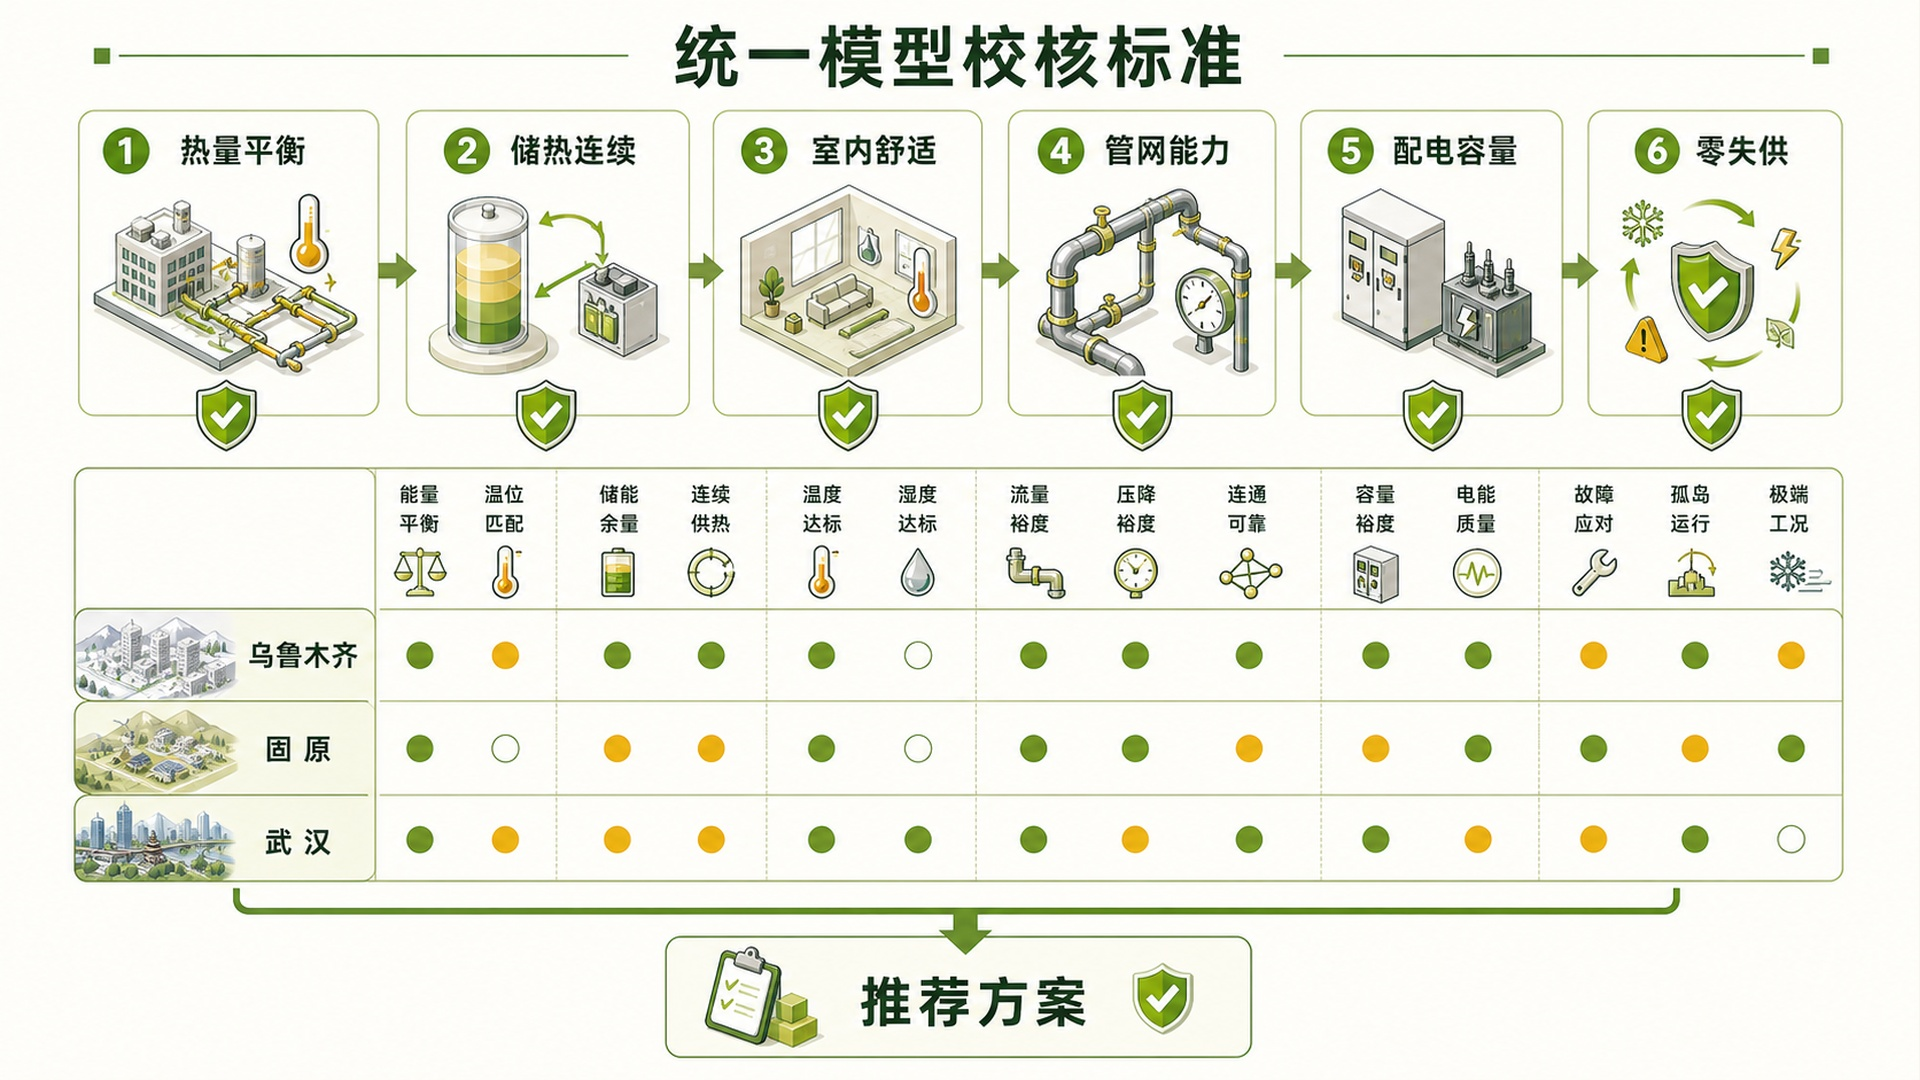
\includegraphics[width=0.62\textwidth,height=0.30\textheight,keepaspectratio]{media/model-cn/16_统一模型校核标准.jpg}
\caption{统一模型校核指标}
\label{fig:model-cn-acceptance}
\end{figure}

上述模型为后续算法提供变量、目标函数和可行域。规划变量确定资产与容量，运行变量描述供暖季逐时状态，工程校核用于确认候选方案满足连续物理边界。

\textbf{全季检验保留小时顺序，建筑与储热状态不逐日重置。}逐时执行守恒及运行边界；典型日仅用于筛选。记录最大残差、超限小时与对象、初末状态和输入版本。聚合案例、逐楼热状态与有限管网反馈分别登记验证范围，结果见数据验证章节。


\clearpage
% !TeX root = ../main.tex
% !TeX program = xelatex
% !TeX encoding = UTF-8
\section{多场景多尺度源荷协同优化方法}\label{minor:algorithm}

本节说明投资与运行的求解顺序、成本碳排权衡及结果检查方法。乌鲁木齐采用联合求解，固原和武汉采用锚定投资后的全季运行校核。算法总体流程如图\ref{fig:alg-overview}所示。

\begin{figure}[H]
\centering
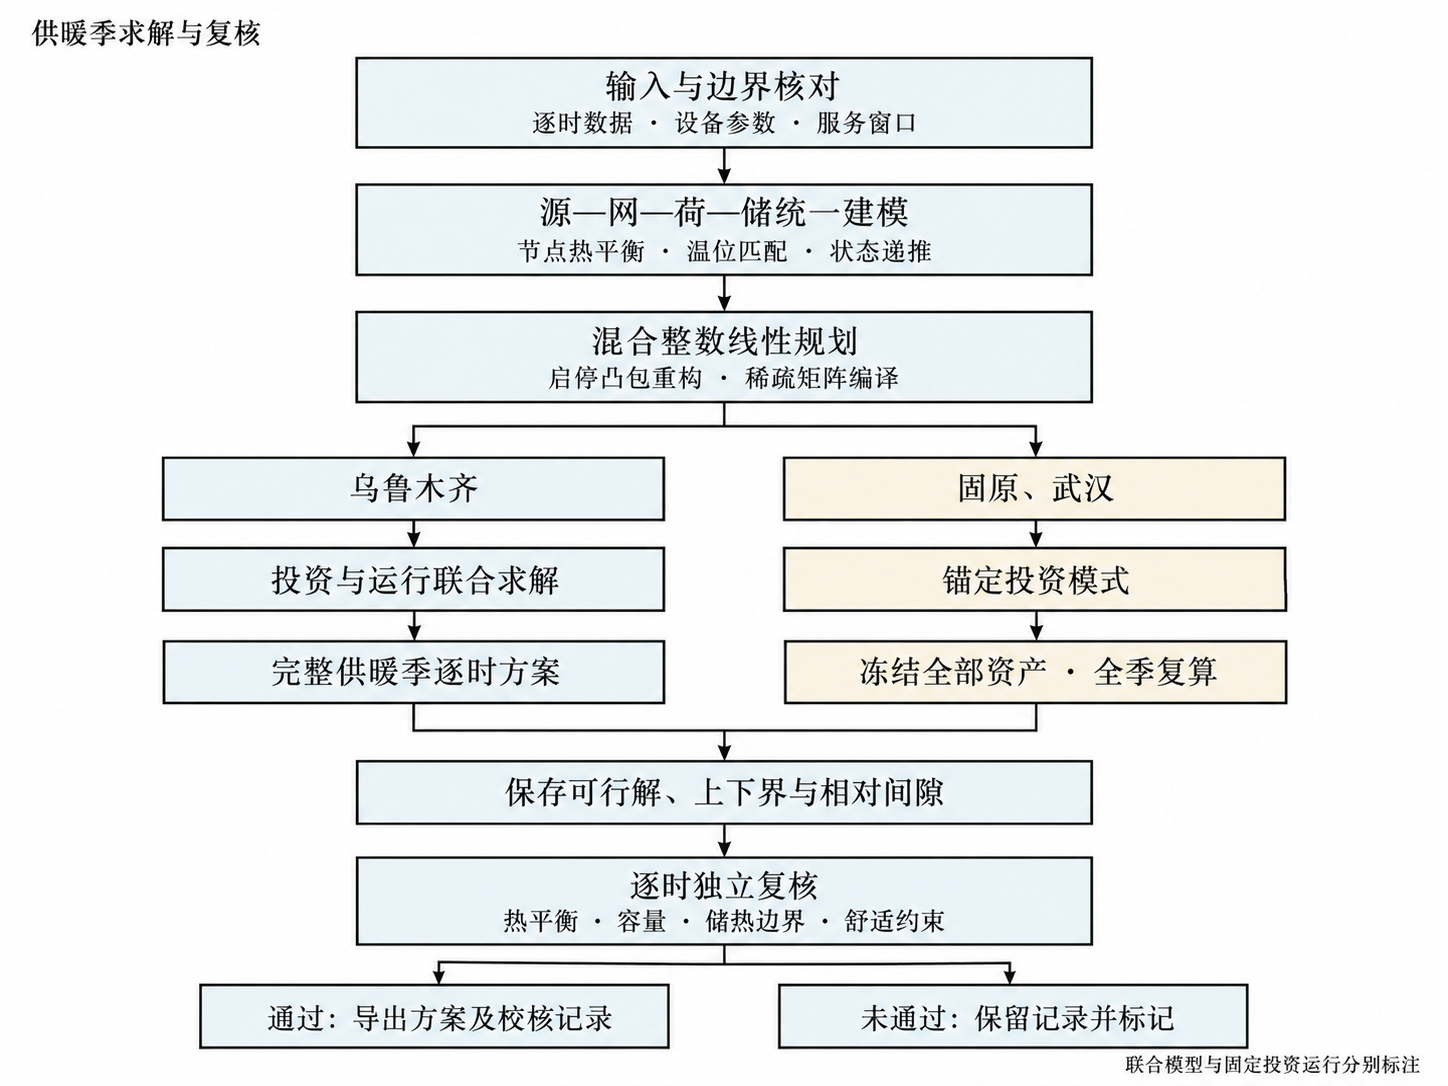
\includegraphics[width=\textwidth]{media/algorithm-revision/season_workflow_a2.png}
\caption{多尺度源荷协同优化算法总体流程}
\label{fig:alg-overview}
\end{figure}

\subsection{方法框架与可复现性}

算法输入包括逐时气象、分时电价、设备与财务参数、城市热网和建筑群画像；输出包括投资方案与逐时调度方案。投资变量涉及设备容量、温位模式、候选管径、储热规模、配电增容和用户侧改造，运行变量包括各热源出力、管网流量与温位、储热状态、需求响应量等。评价指标覆盖成本构成、碳排放、失供量、舒适度偏差和火用损失。

原始三城算例采用1~h时间步长，北京时间左闭右开：乌鲁木齐为2024年10月10日00:00至2025年4月11日00:00，固原为2024年10月15日00:00至2025年4月16日00:00，武汉为2024年11月16日00:00至2025年3月16日00:00，分别为4392~h、4392~h和2880~h。这些历史参数化仿真采用派生负荷及设备、费用假设，用于方法比较。每次求解均记录配置、输入数据指纹、求解状态和相对间隙，以形成可核验的计算记录。

与确定性单情景规划及工程手册式方案比选相比，本文算法的主要差异见表\ref{tab:alg-comparison}。

\begin{table}[H]
\centering
\caption{常见做法与本文算法的对照}
\label{tab:alg-comparison}
\begin{tabularx}{\textwidth}{L{0.27\textwidth}L{0.35\textwidth}Y}
\toprule
常见做法 & 本文算法 & 核验依据\\
\midrule
逐时离散化、确定性单情景规划 & 1~h全季求解，并开展多情景与极端年全年回放 & 主解求解记录、极端年累计61392~h回放\\
采用规划手册指标评价方案 & 单一MILP主解，并进行$\varepsilon$-约束与风险扫描 & 求解状态、上下界和相对间隙\\
规划与运行分开处理 & C1联合求解；C2、C3锚定投资后完成全季运行校核 & 投资层与运行层分别记录状态和间隙\\
\bottomrule
\end{tabularx}
\end{table}

\subsection{多尺度模型}

模型由城市层、区域层和用户层构成，各层通过共享投资变量、逐时运行变量和状态耦合约束连接。三个算例均采用3个模型节点，其中2个为聚合需求节点；乌鲁木齐、固原和武汉分别包含7、6、7类热源和3、2、1条聚合管段。城市层对应总体投资与技术路线，区域层对应热源和输配单元，用户层对应同类建筑负荷的聚合节点。其关系如图\ref{fig:alg-multiscale}所示。

\begin{figure}[H]
\centering
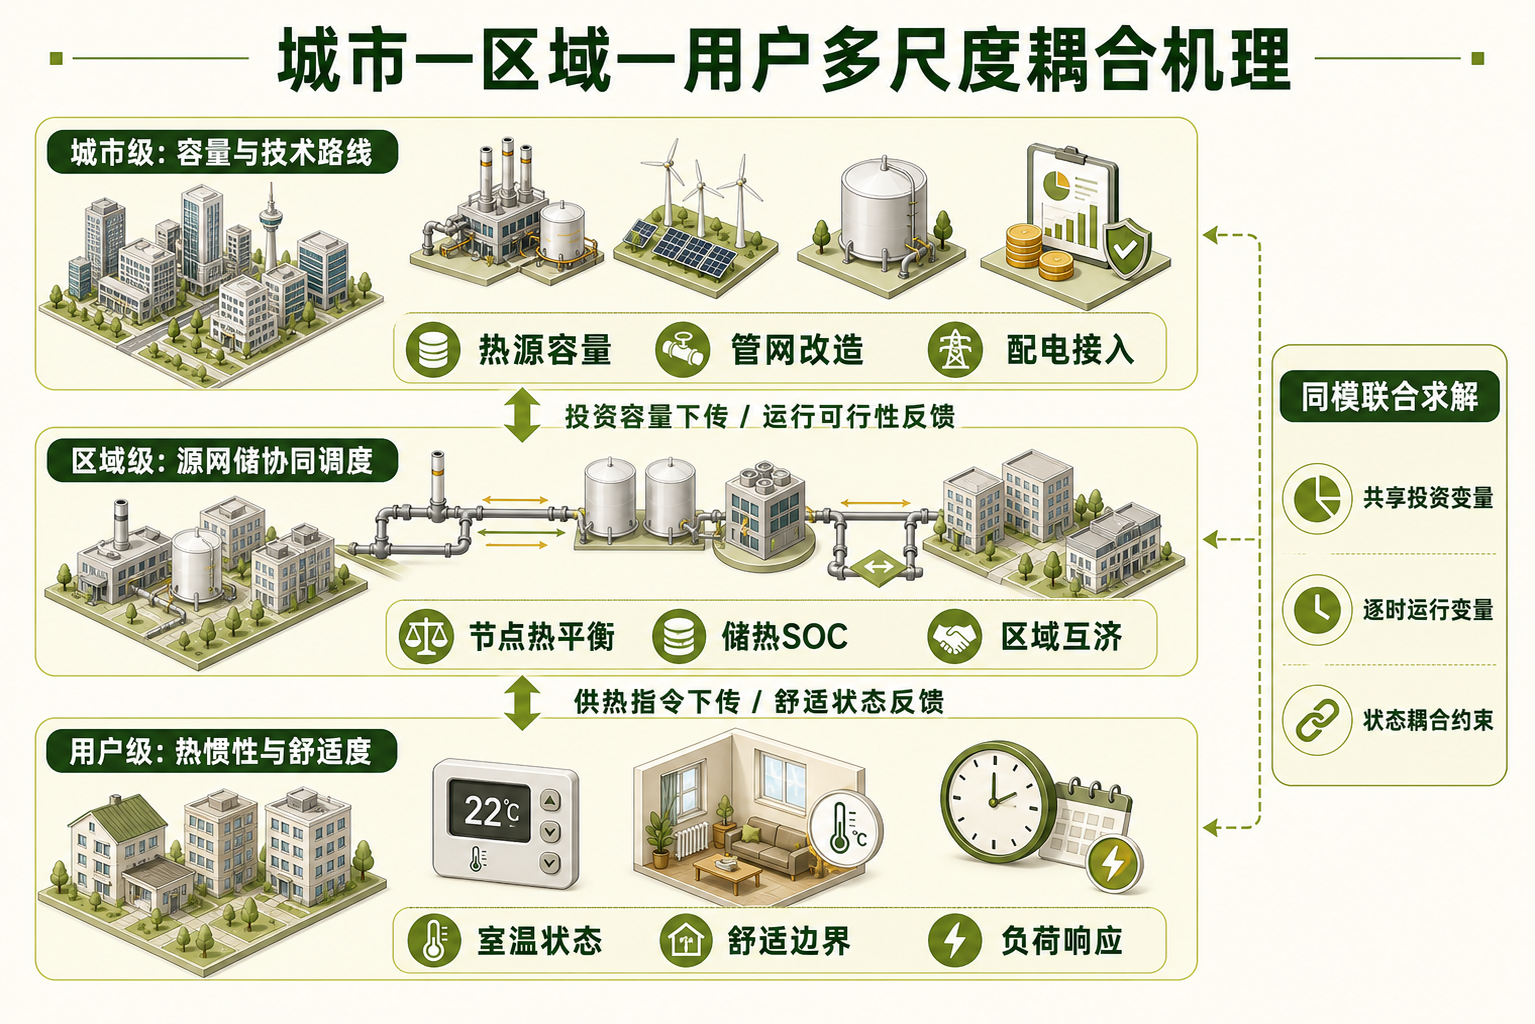
\includegraphics[width=0.76\textwidth,height=0.30\textheight,keepaspectratio]{media/algorithm-revision/fig2.png}
\caption{城市---区域---用户多尺度耦合机制}
\label{fig:alg-multiscale}
\end{figure}

城市层确定容量与技术路线，包括新增或退役机组容量、热源温位模式、候选管径、储热规模以及配电接入和增容。候选技术链依据资源、场地、配电和政策条件生成并预筛，本次计算执行容量、拓扑和温级预审。

区域层描述能流、管网与储热。模型在节点和75/45~$^{\circ}$C两级温位上建立逐时能量平衡。温位兼容约束阻止低温热源直接供应高温需求，高温热源供应低温需求时将品位损失计入火用失配惩罚：
\begin{equation}
T_{\mathrm{src}}^{\min}\geq T_{\mathrm{sup}}+\Delta T_{\mathrm{he}},
\label{eq:alg-grade}
\end{equation}
该不等式用于已选直接供热路径。其中，$T_{\mathrm{src}}^{\min}$为热源供水温度下界，$T_{\mathrm{sup}}$为用户供水温度要求，$\Delta T_{\mathrm{he}}$为换热端差。管网采用温位线性化和双向流动互斥约束，储热状态按下式递推：
\begin{equation}
E_{s,t}=(1-\mu_s)E_{s,t-1}+\eta_{\mathrm{ch}}q_{s,t}^{\mathrm{ch}}\Delta t-\frac{q_{s,t}^{\mathrm{dis}}\Delta t}{\eta_{\mathrm{dis}}},
\label{eq:alg-storage}
\end{equation}
其中，$\mu_s$为自损失率，$\eta_{\mathrm{ch}}$和$\eta_{\mathrm{dis}}$分别为充、放热效率。

用户层描述聚合节点的热惯性与负荷调节。原聚合算例采用前节的单一等效热状态；新增逐楼验证采用精确离散1R1C模型。状态上下界、需求响应窗口守恒和参与率上限共同约束聚合用户侧调节行为。等效热状态递推为
\begin{equation}
E_{n,t}=(1-\lambda_n)E_{n,t-1}+(q_{n,t}^{+}-q_{n,t}^{-})\Delta t,
\qquad \Delta\theta_{n,t}=E_{n,t}/C_n,
\label{eq:alg-building}
\end{equation}
其中，$C_n$为节点$n$的等效热容，$q^+_{n,t}$和$q^-_{n,t}$为相对基准负荷的增加与削减功率。逐楼模型保留供热变化引起的散热变化，按对应算例单独验证。

三个尺度通过容量、温位和建筑改造三类接口耦合：容量约束将运行出力限制在可用率及设备上下限内；温位矩阵完成“源温---网温---节点负荷”匹配；用户侧调节量先进入节点热平衡，再由热源出力与储热充放共同响应。例如在已有逐时结果中，用户侧负荷削减使同一时段节点需求下降，优先减少边际热源出力；恢复负荷出现时，由储热与可调热源按相应解共同响应，节点平衡在每个时段保持闭合。乌鲁木齐场景采用投资---运行联合MILP；固原和武汉因问题规模采用锚定两阶段方法，先确定投资模式，再冻结投资开展全季运行校核。因此，后两个场景的推荐方案用于工程可行性比较，不将投资层结果表述为全局最优。

\subsection{多目标协同优化}\label{minor:multiobjective}

成本与碳排放采用$\varepsilon$-约束法协调\supcite{32}。费用目标仍保留场景配置的碳价和偏好项；仅专用无碳价入口以基本费用形成比较。模型以全生命周期净成本的等年值最小为目标，同时设置碳排放上限；逐档收紧上限并重新求解完整供暖季，相邻两档的成本增量与减排量之比用于计算边际减排成本。

乌鲁木齐场景中，成本端点为27.49万元、27.32~t~CO$_2$，排放端点为74.81万元、10.57~t~CO$_2$。本文推荐记录采用通过该记录已启用硬约束与校核的方案，等年值成本为27.76万元、碳排放为27.31~t~CO$_2$；该记录与仅按目标函数排序得到的成本端点分开标注。单位供热成本由基准方案的0.078851元/kWh增至0.100681元/kWh，增加27.69\%。该增幅反映以成本增加换取减排、清洁热利用和可靠性约束的综合取舍。

零失供、清洁热比例、N$-1$容量裕度及对应热状态上下限按已启用配置作为硬边界，不与经济性目标交换；地源年度平衡保留为可选约束。失供率约束为
\begin{equation}
U_{\mathrm{un}}=\frac{\sum_t q_t^{\mathrm{un}}}{\sum_t Q_t}\leq U_{\max},
\label{eq:alg-unserved}
\end{equation}
其中，$q_t^{\mathrm{un}}$为失供功率，$Q_t$为热需求，$U_{\max}=0$表示推荐方案不允许失供。边界内的需求移峰和舒适偏差通过惩罚成本进行优化。

气象不确定性作为独立风险层，采用
\begin{equation}
\min\ \mathbb{E}[C]+\lambda\operatorname{CVaR}_{\alpha}(C),
\qquad \alpha=0.8,
\label{eq:alg-risk-objective}
\end{equation}
其中，$\lambda$取0、0.02、0.05和0.10四档。条件风险价值采用Rockafellar--Uryasev线性化：
\begin{equation}
\operatorname{CVaR}_{\alpha}(C)=\min_{\eta,z_s}\left\{\eta+\frac{1}{1-\alpha}\sum_s p_sz_s\right\},
\quad z_s\geq C_s-\eta,\quad z_s\geq0.
\label{eq:alg-cvar}
\end{equation}

$\lambda=0.05$作为三个场景的统一参考值。多气象年风险层中，乌鲁木齐的期望成本增加0.012万元、CVaR下降0.831万元；固原的期望成本增加0.016万元、CVaR下降0.515万元，变化约占年化成本的0.01\%。武汉场景的投资不随风险权重改变，说明其投资方案主要由硬约束决定。不同风险权重下的结构变化见表\ref{tab:alg-lambda}。

\begin{table}[H]
\centering
\caption{多气象年风险层的$\lambda$权重扫描结果}
\label{tab:alg-lambda}
\begin{tabularx}{\textwidth}{cYYY}
\toprule
$\lambda$ & 乌鲁木齐 & 固原 & 武汉\\
\midrule
0.02 & 余热源热泵、备用电锅炉和配电容量首次调整 & 投资配置不变 & 投资配置不变\\
0.05 & 继续小幅调整 & 储热与微网可再生增加，生物质调峰减少 & 投资配置不变\\
0.10 & 进一步转入风险平衡 & 与0.05档接近 & 投资配置不变\\
\bottomrule
\end{tabularx}
\end{table}

$\lambda$扫描来自2020---2024多气象年全年回放，用于风险机制专项验证；供暖季主结果中的成本---碳Pareto采用确定性单情景计算。风险层共包含12个规划案例（3个场景$\times$4档$\lambda$），全部收敛，60项年度容量审计通过，CVaR台账一致性误差为$5.59\times10^{-9}$元。图\ref{fig:alg-objectives}展示的是该专项风险层的12/12案例收敛与60/60容量审计结果，不等同于供暖季推荐方案的13道机器验收。

\begin{figure}[H]
\centering
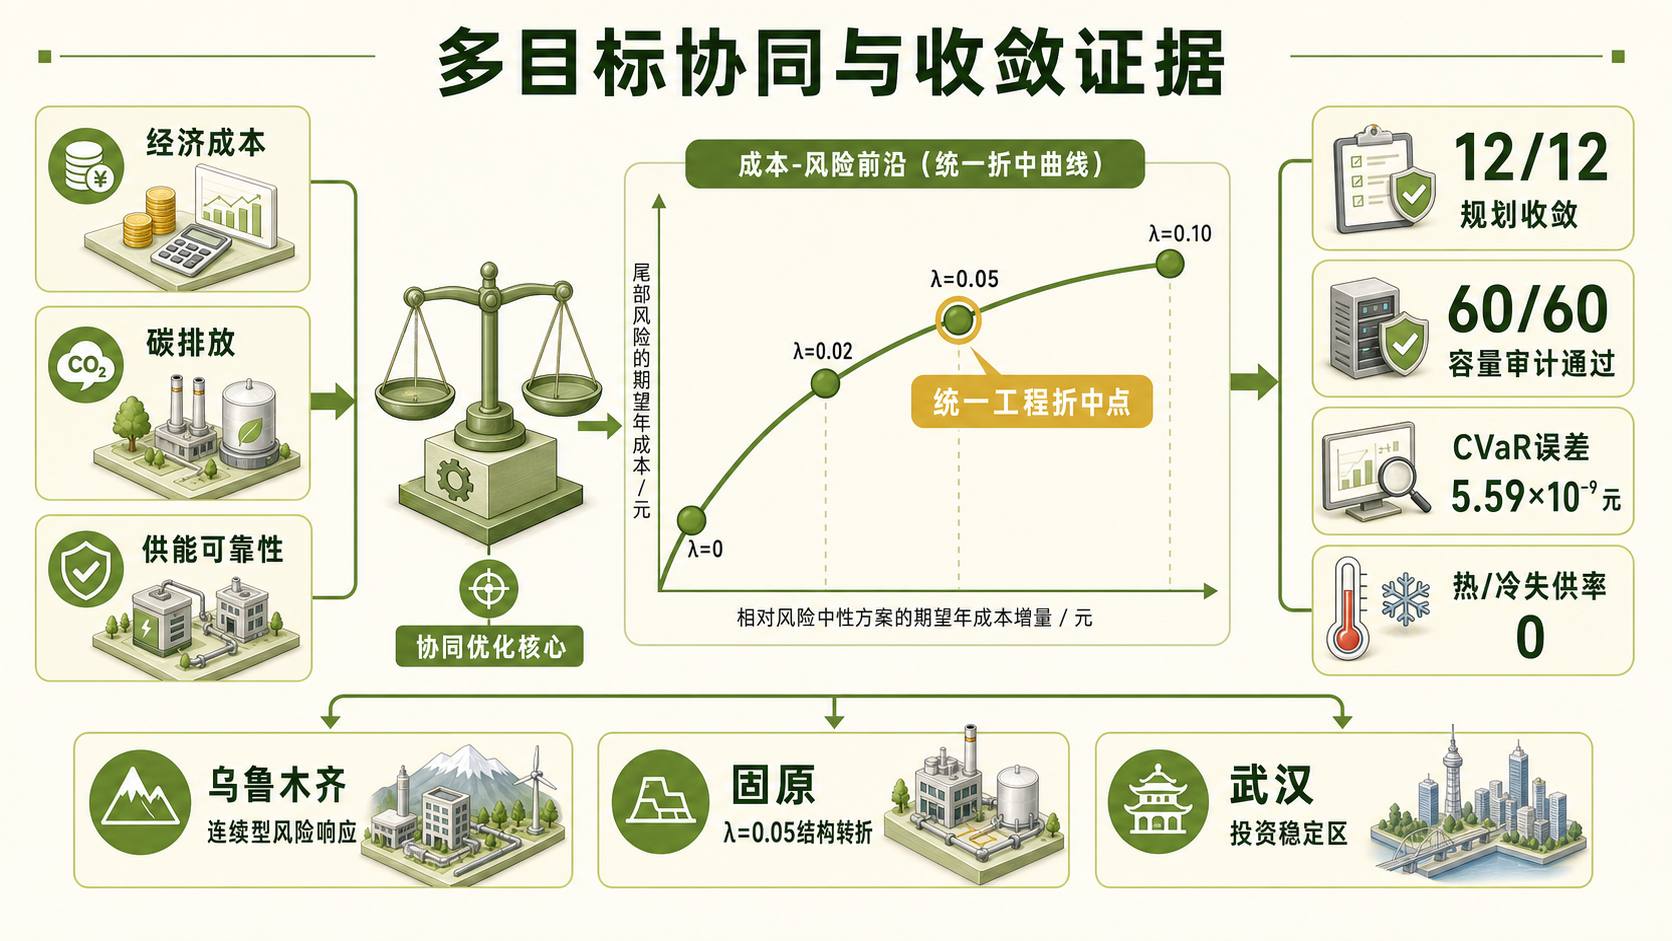
\includegraphics[width=0.76\textwidth,height=0.30\textheight,keepaspectratio]{media/algorithm-revision/fig3.png}
\caption{多目标协同与风险层收敛证据}
\label{fig:alg-objectives}
\end{figure}

\subsection{求解流程与收敛准则}

模型构造器采用Python~3.11实现，并通过SciPy的\texttt{milp}接口调用HiGHS求解。约束矩阵按CSR/CSC稀疏格式编译和缓存，模型装配约需1.6~s，未使用自定义割。机组启停采用凸包重建模，开机状态保留为二元变量，启动和停机辅助变量连续化。全年回放单城测试中，整数变量数量由26280个减至8760个。

算法\ref{alg:season-workflow}给出主结果的求解与校核顺序，算法\ref{alg:epsilon-workflow}给出独立碳帽扫描。优化器一次求解整个声明窗口，小时索引用于建立守恒与状态约束。求解状态、相对间隙、约束残差和后验校核分别登记；时限内可行解保留其近似解身份。附录3列出与这些步骤对应的真实Python代码节选。

% !TeX root = ../main.tex
\newcounter{paperalgorithm}
\newenvironment{paperalgorithm}[2]{%
  \par\Needspace{15\baselineskip}\refstepcounter{paperalgorithm}\label{#2}%
  \begingroup\small\setstretch{1.05}\setlength{\parskip}{4pt}%
  \noindent\rule{\linewidth}{0.6pt}\par\noindent\textbf{算法\thepaperalgorithm\quad #1}\par
}{\par\noindent\rule{\linewidth}{0.6pt}\par\endgroup}

\begin{paperalgorithm}{供暖季求解与复核流程}{alg:season-workflow}
\noindent\textbf{输入：}场景配置、规划输入、连续供暖季逐时数据和求解容差。\par
\noindent\textbf{输出：}投资及逐时运行方案，求解状态、间隙和校核记录。
\begin{enumerate}[label=\arabic*.,leftmargin=1.8em,itemsep=2pt,topsep=3pt,parsep=0pt]
\item 核对时间范围、步长、缺测及单位；读取各模块启用状态与参数来源。
\item 装配源、网、荷、储及电力接口；对所有小时联立守恒、容量和热状态约束，设置初始及期末边界。
\item \textbf{若采用联合求解：}在完整声明窗口同时求投资与运行方案。
\item \textbf{若采用固定投资复算：}求得规划方案或读入已登记方案；将全部投资项冻结为存量，保持可靠性条件，再构造全季运行模型并求解。
\item 保存可行解、求解状态、上下界及相对间隙；无可行解时随异常报告失败原因，结束本次计算。
\item 按实际启用模块，复核逐时平衡、容量、储热边界、舒适约束与服务期覆盖；校核不通过则保留记录并标记未通过。
\item 导出配置、投资、逐时运行与检查结果；分别标注联合模型可行解或固定投资下可行解。
\end{enumerate}
\end{paperalgorithm}

\begin{paperalgorithm}{独立费用—碳排放采样接口}{alg:epsilon-workflow}
\noindent\textbf{输入：}同一配置和时间序列、碳帽档数$K\geq2$。\par
\noindent\textbf{输出：}通过复核的采样非支配方案、边际减排费用和折中建议。
\begin{enumerate}[label=\arabic*.,leftmargin=1.8em,itemsep=2pt,topsep=3pt,parsep=0pt]
\item 复制输入配置，清除原碳帽并令碳价为零；保留设备、运行与可靠性约束。
\item 分别以费用和排放为主目标求端点；第二阶段约束主目标不高于第一阶段可行值加容差，再优化次目标。
\item 检查端点排放的先后关系；不满足容差要求则终止，满足时在两端排放值间等距设置$K$档碳帽。
\item \textbf{对每档碳帽：}复制同一基础配置，加数值容差后施加碳帽；按费用目标重新构模并求解。投资项是否固定取决于输入配置。
\item 对本档解独立检查数值残差和碳帽；任一检查不通过则报错并终止扫描，通过则保存全部结果。
\item 对通过的样本去重并剔除受支配点，计算相邻方案的边际减排费用；用归一化理想点距离给出折中建议。
\end{enumerate}
\end{paperalgorithm}

算法\ref{alg:epsilon-workflow}对应当前代码的独立接口，流程见图\ref{fig:epsilon-workflow-a2}。所得集合限于已采样可行解，折中建议取决于归一化规则。供暖季历史扫描保留其原记录中的碳价与偏好，不与这一接口混记。

\begin{figure}[H]
\centering
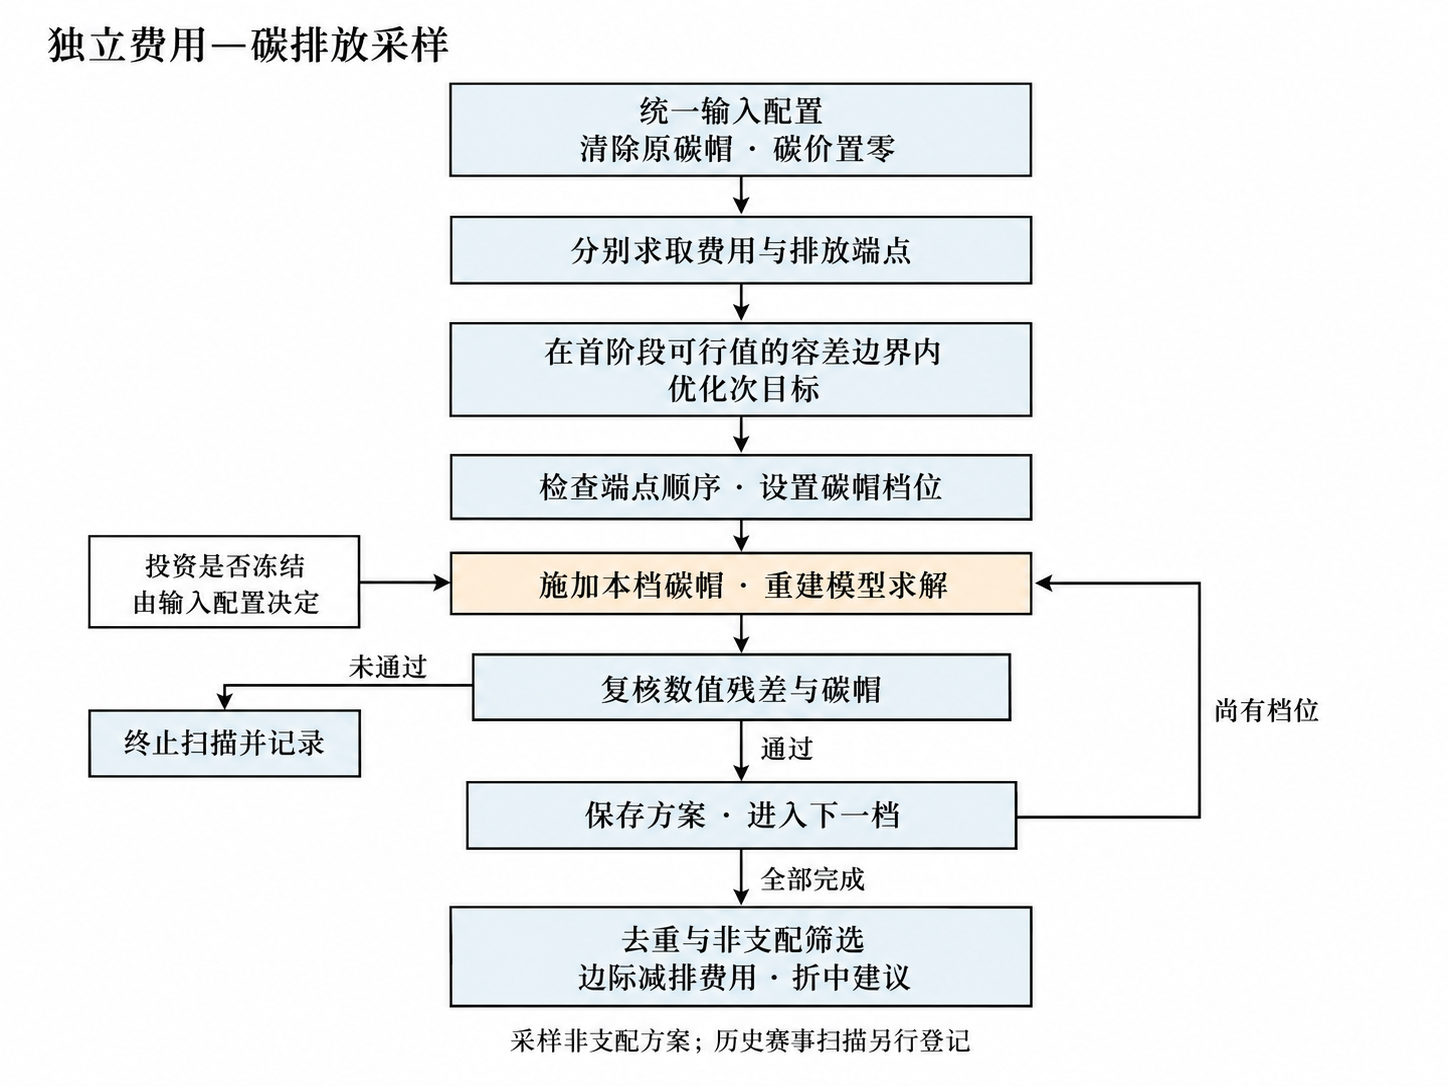
\includegraphics[width=\textwidth]{media/algorithm-revision/epsilon_workflow_a2.png}
\caption{独立费用---碳排放采样与复核流程}
\label{fig:epsilon-workflow-a2}
\end{figure}


乌鲁木齐联合模型的相对间隙为$1.53\times10^{-4}$；固原锚定投资后的运行层间隙为$1.84\times10^{-3}$；武汉运行层为连续规划，间隙为0，其投资层记录为0.98\%。三场景逐时热平衡最大绝对残差依次为$7.41\times10^{-13}$、$1.25\times10^{-10}$和$8.53\times10^{-14}$~kW，均低于$10^{-6}$~kW容差。投资层、运行层与机器验收分别留存状态，不将固原和武汉表述为联合求解通过。结果见表\ref{tab:alg-solver}。

\begin{table}[H]
\centering
\caption{三场景推荐方案求解与验收结果}
\label{tab:alg-solver}
\small
\begin{tabularx}{\textwidth}{@{}L{0.11\textwidth}L{0.20\textwidth}L{0.18\textwidth}L{0.09\textwidth}L{0.14\textwidth}Y@{}}
\toprule
场景 & 求解方法 & 整数变量 & 时间/s & 相对间隙/\% & 结果属性\\
\midrule
乌鲁木齐 & 投资---运行联合MILP & 启停二元8784个 & 531.1 & 联合层0.0153 & 联合模型可行解\\
固原 & 锚定两阶段 & 运行层启停二元4392个 & 64.0 & 运行层0.184 & 固定投资下可行解\\
武汉 & 锚定投资+连续运行 & 0 & 31.7 & 运行层0；投资层0.98 & 固定投资下可行解\\
\bottomrule
\end{tabularx}
\end{table}

敏感性测试的20档扰动获得有效解，其中乌鲁木齐电价高档和余热低档为时间受限近似解，相对间隙分别为7.05\%和9.44\%；另有固原负荷低档、武汉碳价高档两档未收敛。乌鲁木齐Pareto中间档的部分点在时限内间隙为13.2\%---13.7\%。固原三档采用推荐投资模式复算，全部满足碳排放上限，间隙为0.20\%、0.22\%和0.24\%，这些结果属于冻结投资模式的运行参考点，不代表完整联合MILP重新寻优。

为检验乌鲁木齐排放端点投资模式在不同碳帽下的运行可达性，固定排放端点记录的投资、退役、管径、储热和末端改造模式，对23365、19136和14906~kg三档碳帽进行全季运行重算。三档实际排放均为10616.5~kg，失供率为0，求解状态均为Optimal，相对间隙为$1.90\times10^{-7}$。运行成本为11.271万元/年，仅包含运行费用，不与联合解中包含资本成本的Pareto结果直接比较。

\subsection{计算效率与扩展性}

求解效率的改善主要来自启停凸包重建模和稀疏编译缓存。固原全年回放用时由575.746~s降至86.903~s，提升6.63倍；两年度合计用时由602.483~s降至112.750~s，减少81.29\%。该结果来自多气象年全年回放的单城效率测试。单次供暖季问题约包含31万---45万个变量，乌鲁木齐场景的启停二元变量为8784个。连续温位、C\&CG、Benders分解和在线MPC作为可选扩展，本次计算未启用。逐时回放、边界检验和求解加速关系如图\ref{fig:alg-replay}所示。

\begin{figure}[H]
\centering
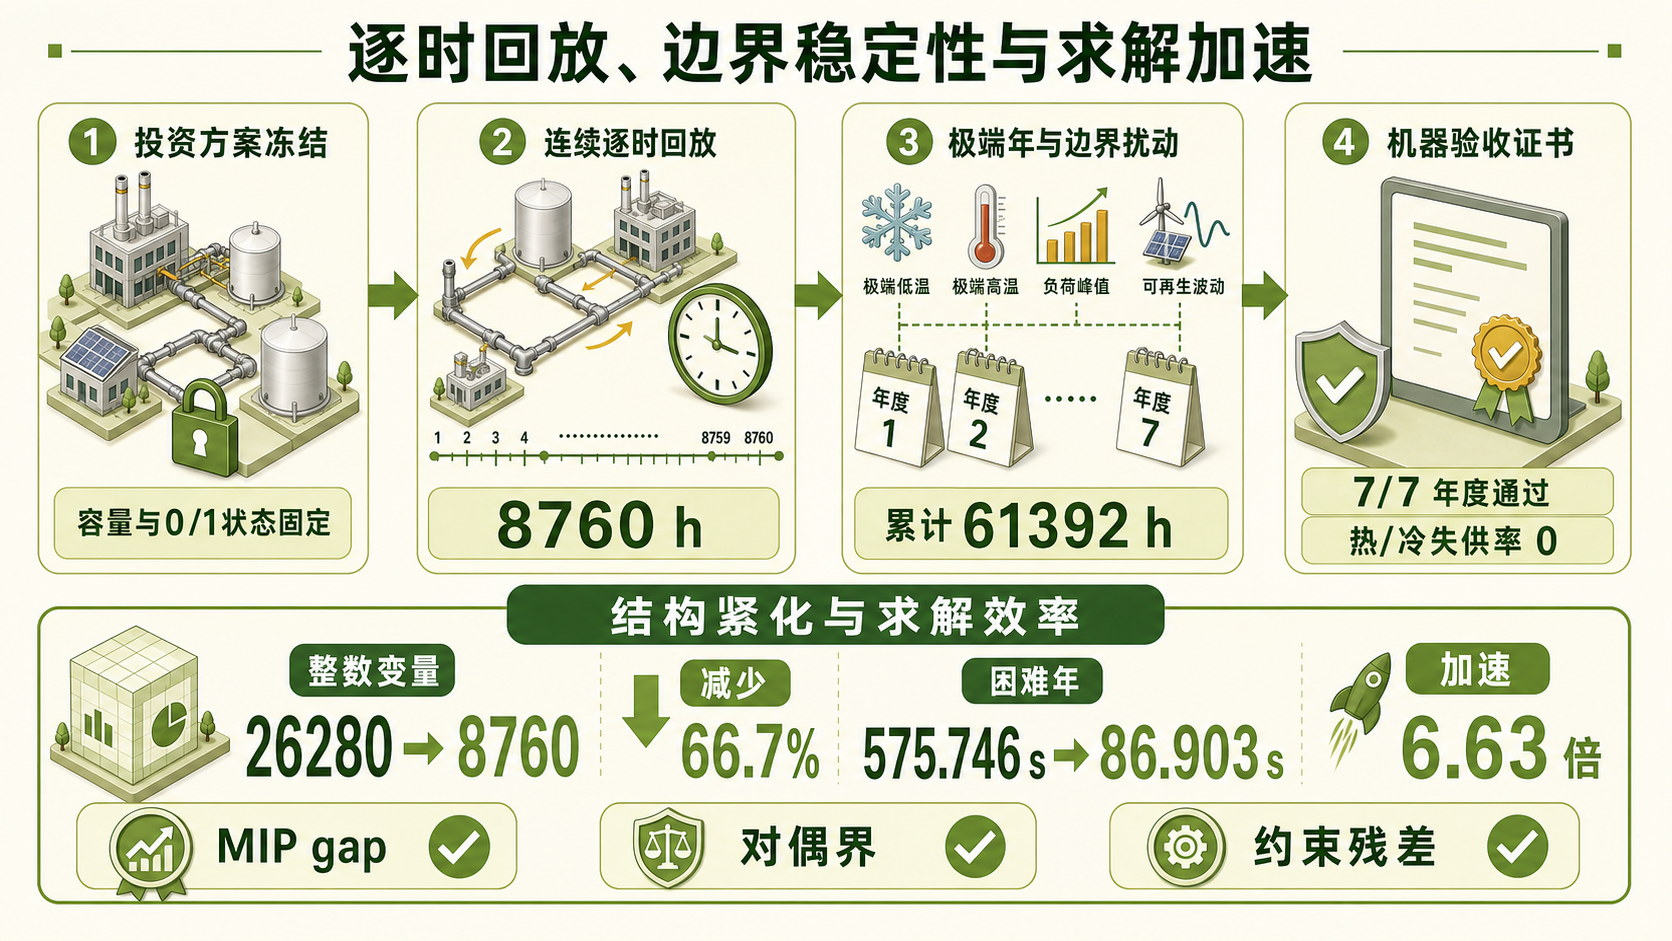
\includegraphics[width=0.76\textwidth,height=0.30\textheight,keepaspectratio]{media/algorithm-revision/fig4.png}
\caption{逐时回放、边界稳定性与求解效率}
\label{fig:alg-replay}
\end{figure}

\subsection{数值结果与敏感性}

图\ref{fig:code-kpi}比较了基准方案与推荐方案的成本、碳排放、清洁热利用和供热可靠性指标。推荐方案的取舍由成本、排放上限、清洁热占比和供热约束共同决定，因此各项指标的变化方向并不完全一致。图中成本采用年化等效口径，单位供热成本按交付热量折算，二者与供暖季现金运行成本分别核算。

\begin{figure}[H]
\centering
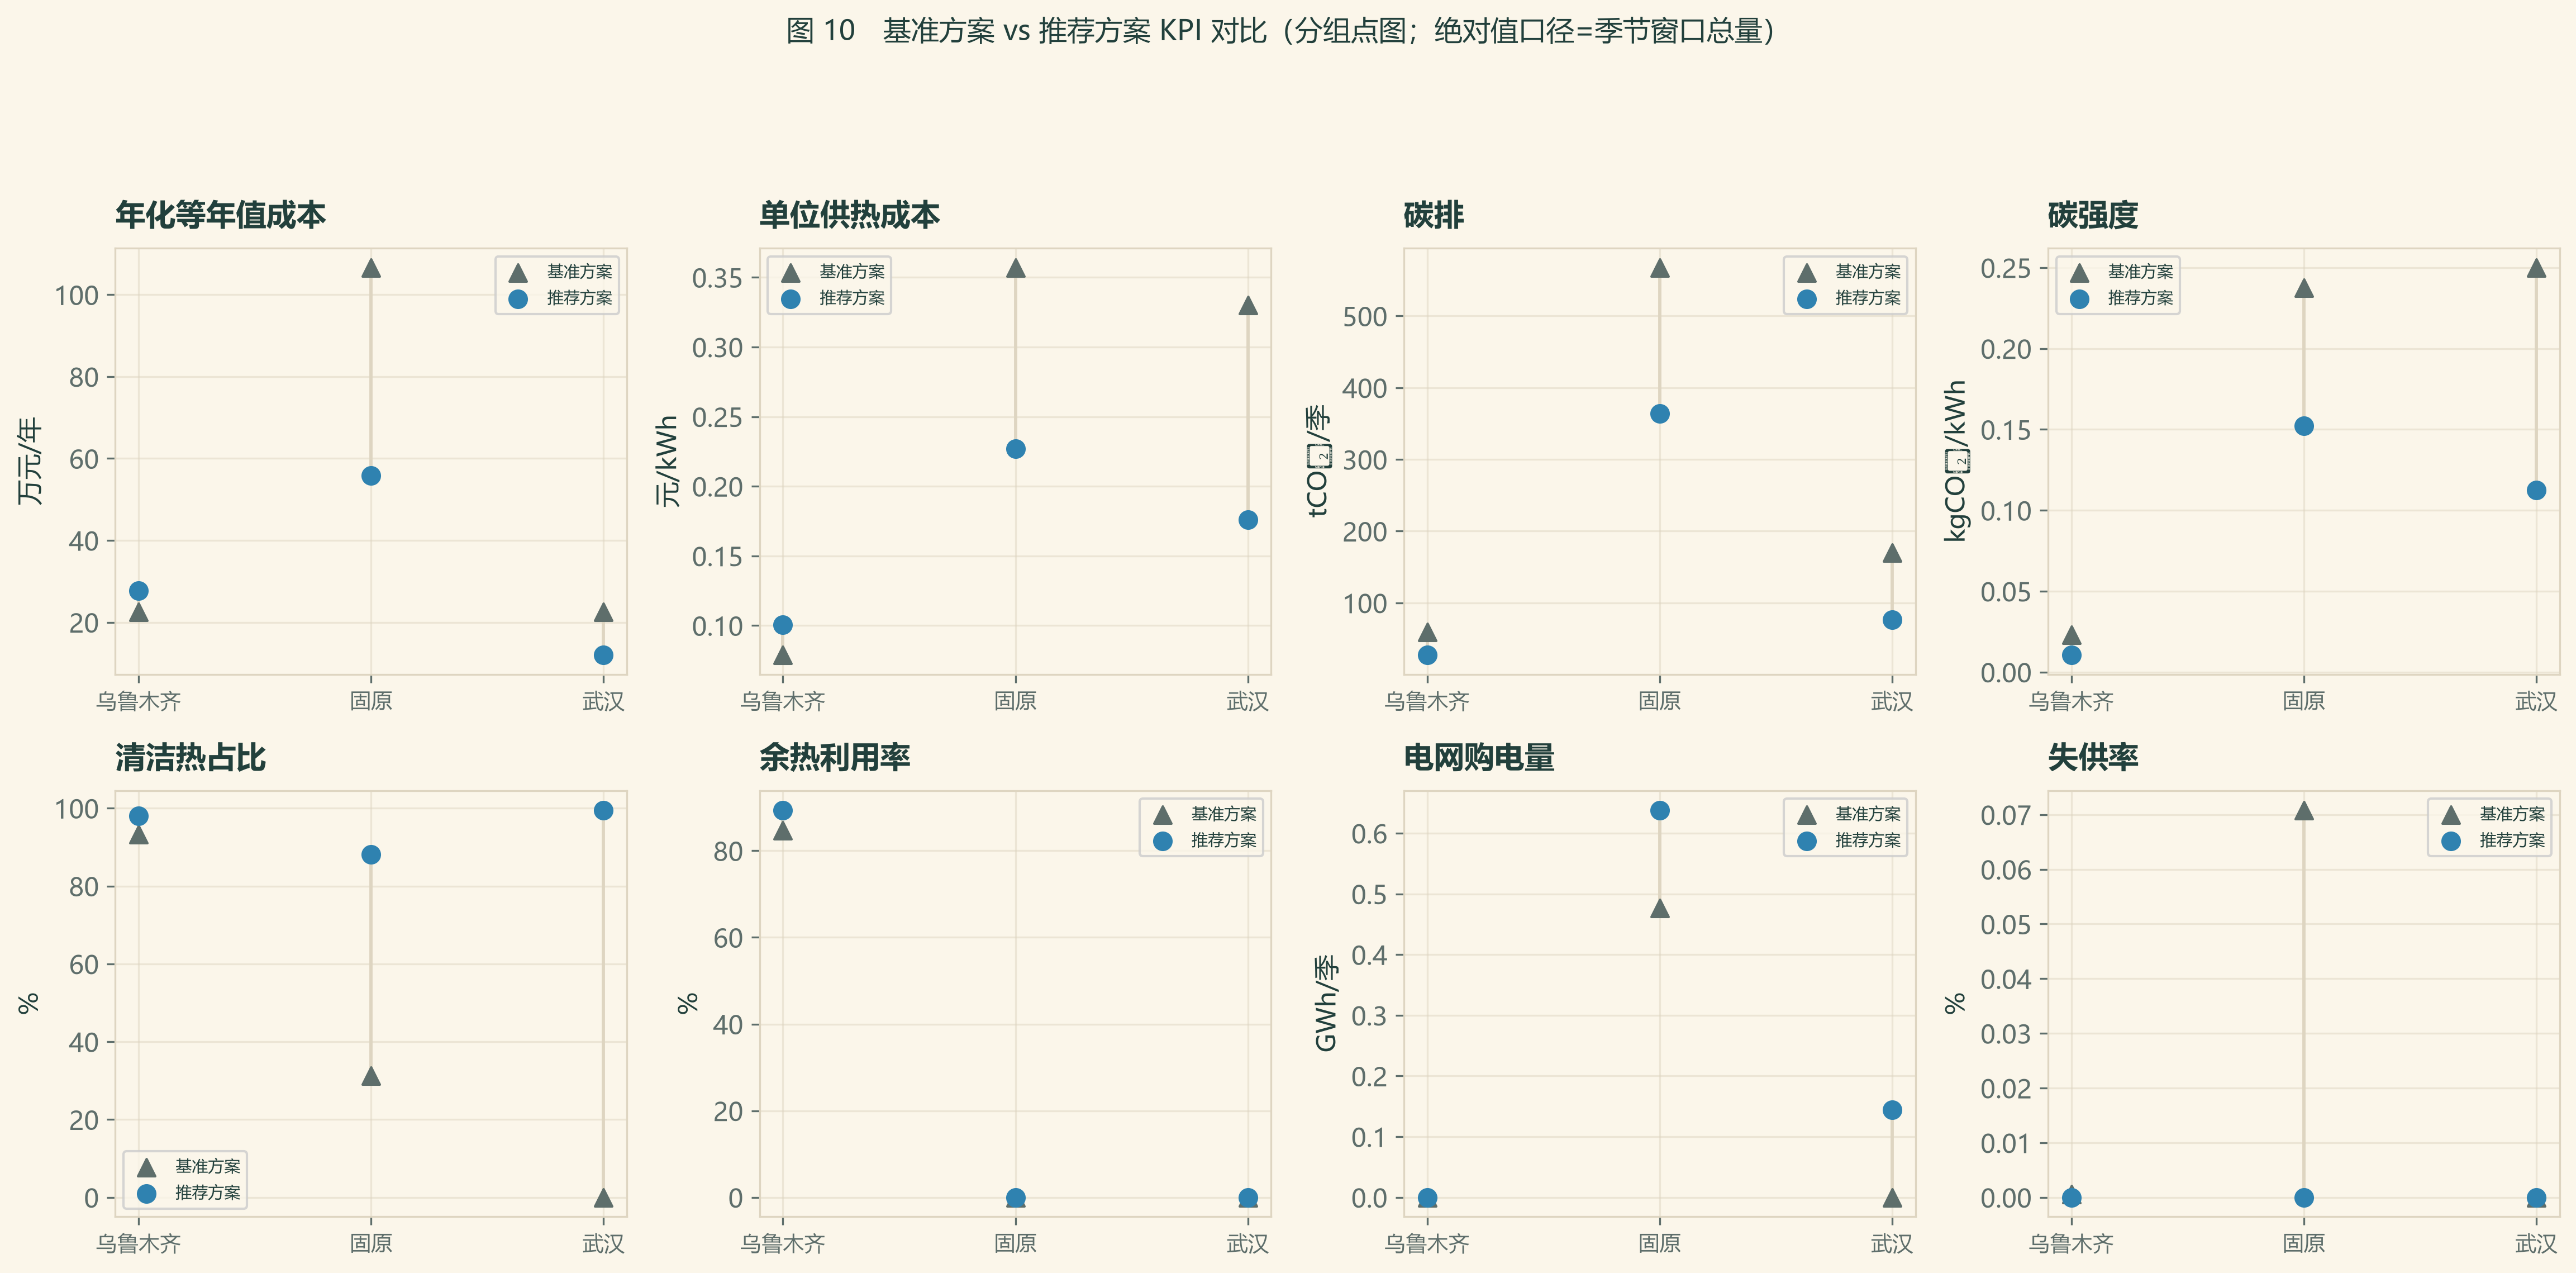
\includegraphics[width=0.98\textwidth,height=0.52\textheight,keepaspectratio,trim=0 0 0 100,clip]{media/code-results/fig10_kpi_comparison.png}
\caption{基准方案与推荐方案KPI对比}
\label{fig:code-kpi}
\end{figure}

成本与碳排放的候选解分布见图\ref{fig:code-pareto}。推荐方案从满足排放、可靠性和投资边界的候选解中选取，不必与最低成本点或最低排放点重合。部分点为固定投资模式下的运行参考点或时限内近似解，其求解状态和相对间隙以前文说明为准。

\begin{figure}[H]
\centering
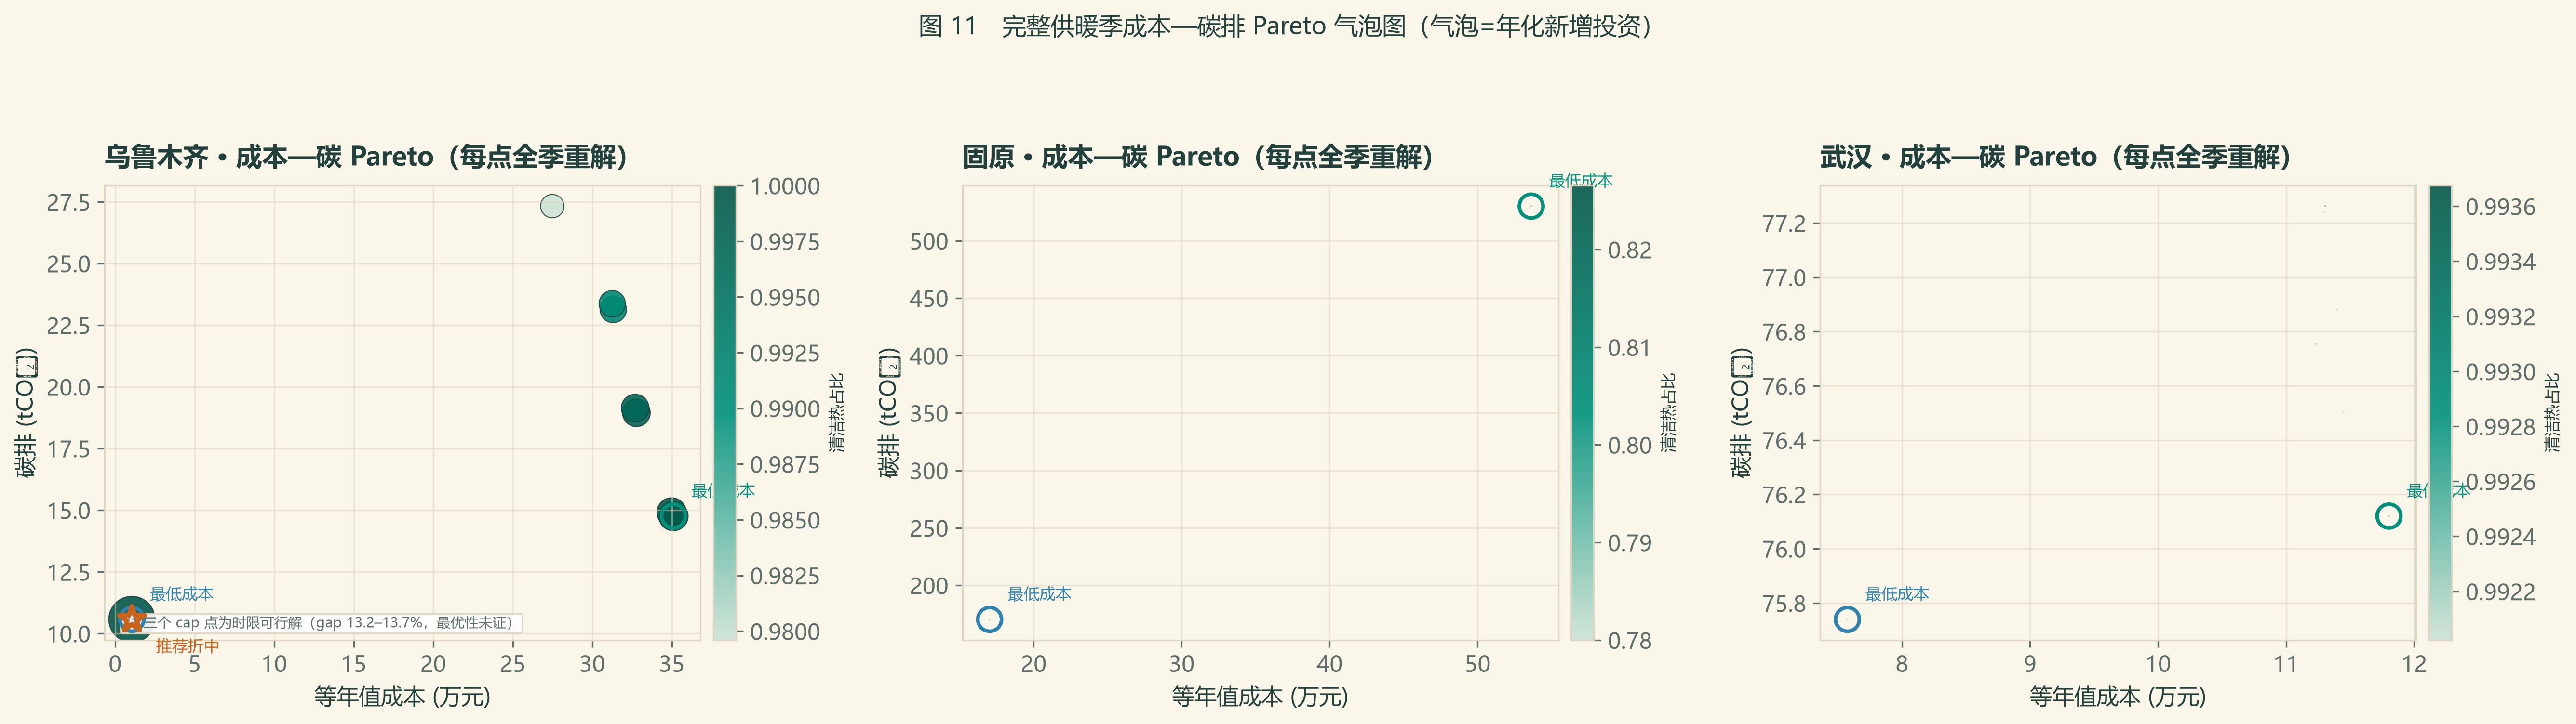
\includegraphics[width=0.78\textwidth,height=0.33\textheight,keepaspectratio,trim=0 0 0 100,clip]{media/code-results/fig11_cost_emission_pareto.png}
\caption{三城市成本—碳排放候选方案对比}
\label{fig:code-pareto}
\end{figure}

V4全年单情景消融实验沿用原时间权重，并在每次移除模块后重新求解投资与运行。完整模型的年化目标为95.620万元，碳排放为30.602万kg~CO$_2$。去掉需求响应后，年化成本增加0.09\%，购电量增加0.21\%；去掉新增储热后，年化成本增加3.55\%，碳排放增加6.05\%，购电量增加3.41\%；去掉火用失配惩罚后，火用损失增加4.90\%。该组结果用于检验V4模块贡献，与三城市供暖季推荐方案分开报告。

复合寒潮压力测试沿用V4算例，将室外温度序列整体降低8~$^{\circ}$C、负荷提高15\%、余热可用量降低15\%，并冻结投资变量。测试结果仍保持零失供；按同一能源运行费口径，费用由50.057万元增至100.349万元，增加100.47\%，购电量增加56.78\%，碳排放增加113.95\%。逐档敏感性分析表明：乌鲁木齐对热负荷最敏感，成本变化为$+19.1\%/-17.9\%$，其次为余热下降和电价上升；固原的生物质到货扰动因库存缓冲未改变成本；武汉对电价和热负荷较敏感，变化范围分别为$+16.9\%/-14.6\%$和$+16.8\%/-13.7\%$。

最冷连续168~h的热源出力、负荷和储热状态见图\ref{fig:code-cold168}，用于检查低温持续期间的逐时供需平衡。图\ref{fig:code-worst72}进一步列出最不利72~h窗口内的可用供热能力、负荷、储热与容量裕度。两图分别反映常规极寒时段调度和压力场景下的边界状态，不据此假定三城市具有相同的储热运行模式。

\begin{figure}[H]
\centering
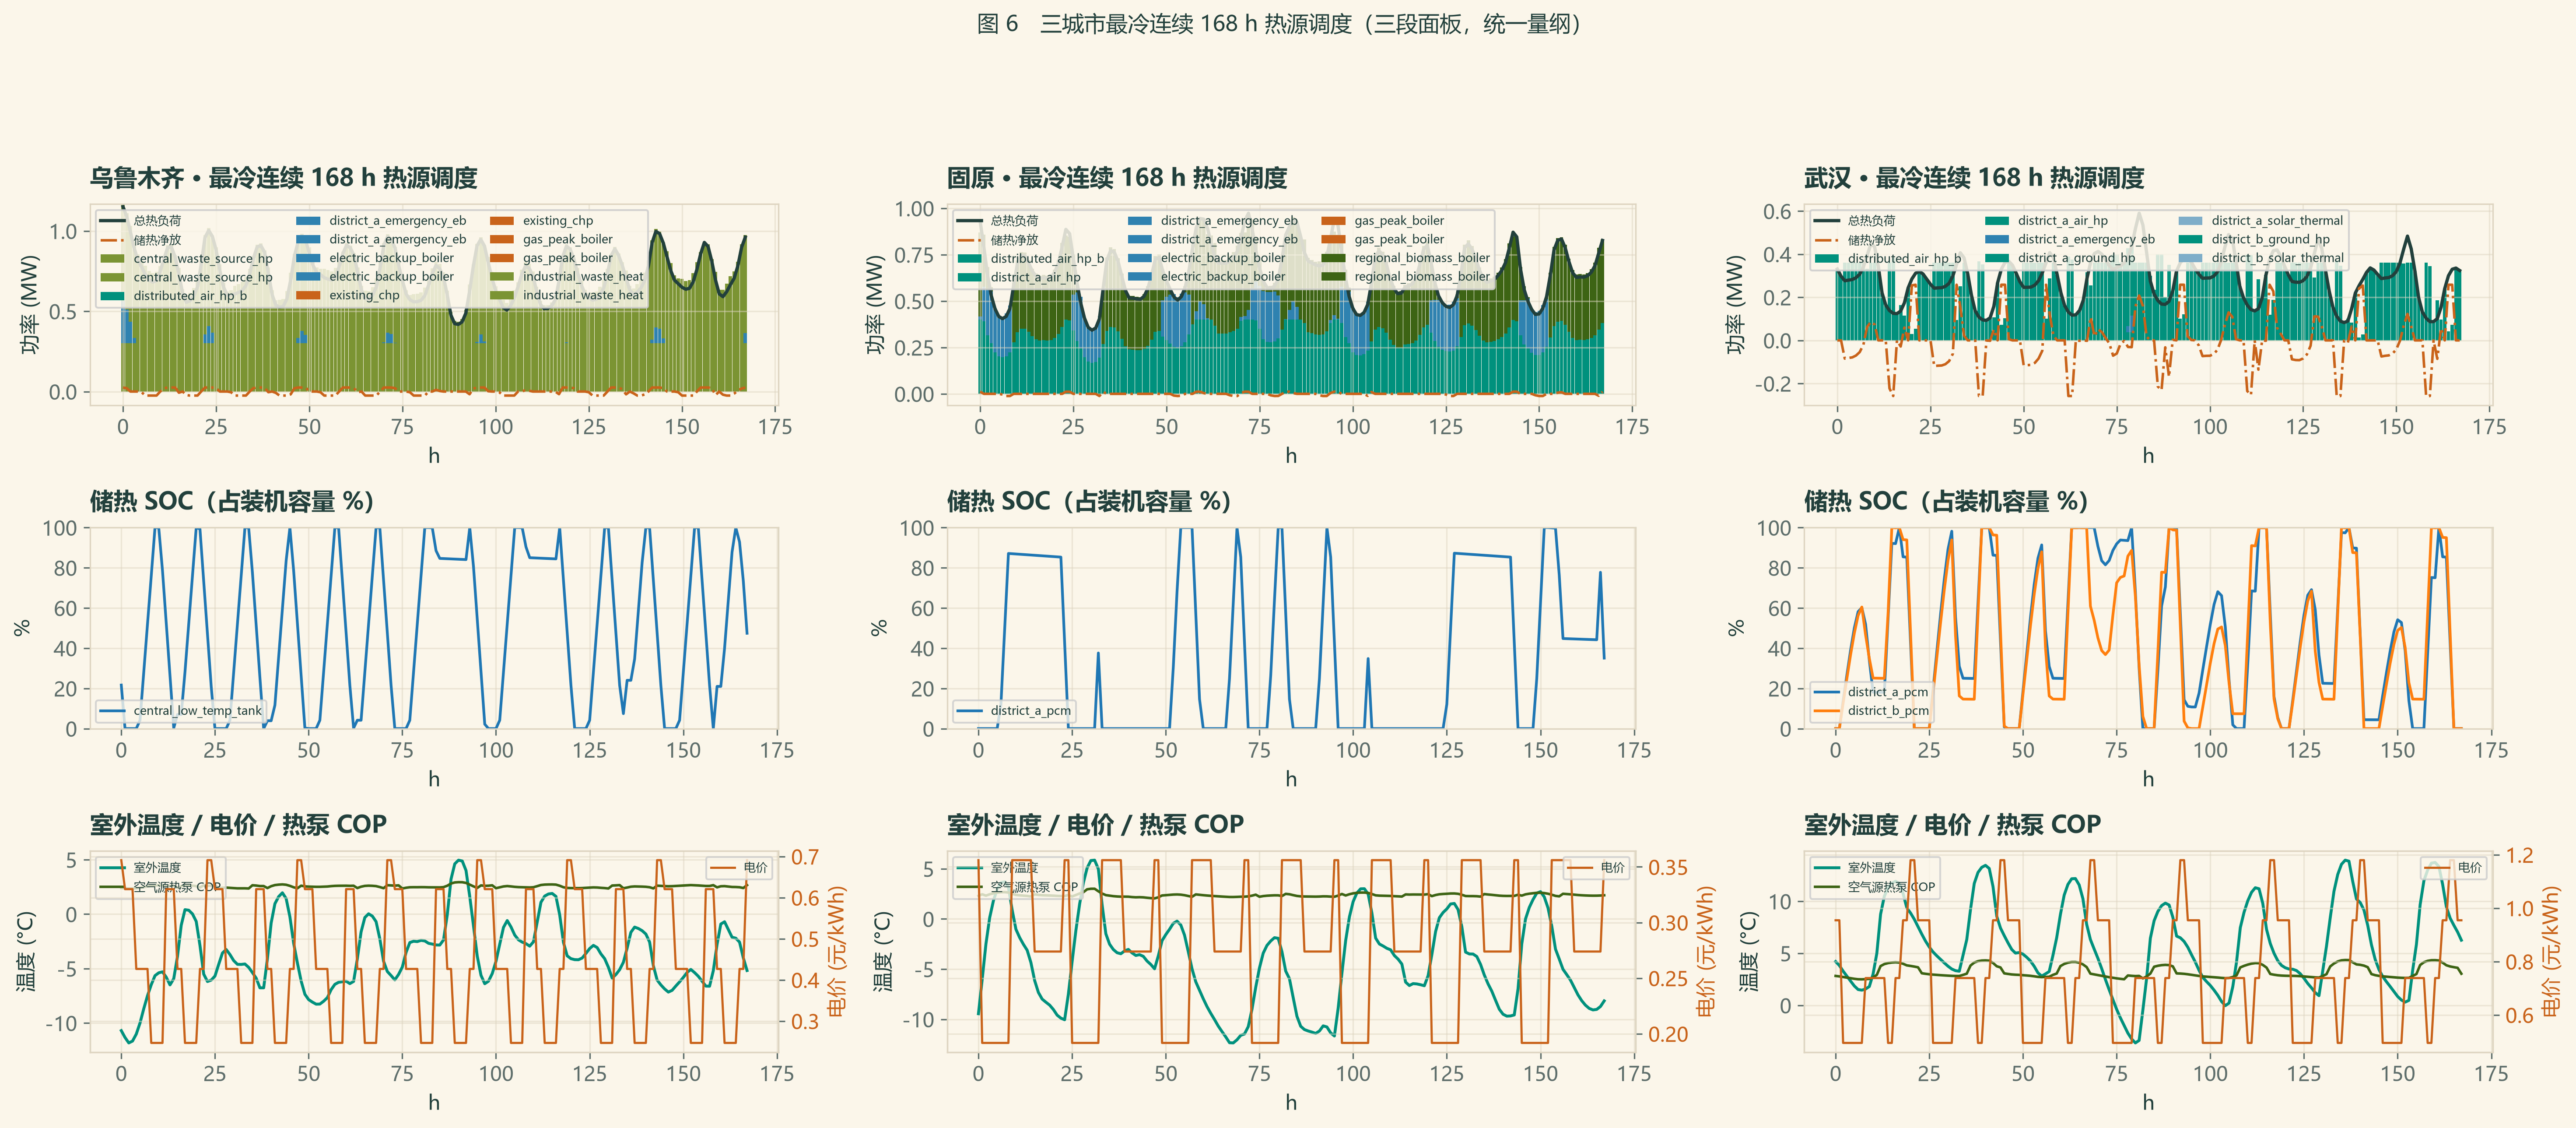
\includegraphics[width=0.98\textwidth,height=0.54\textheight,keepaspectratio,trim=0 0 0 100,clip]{media/code-results/fig06_coldest_168h_dispatch.png}
\caption{最冷连续168 h调度}
\label{fig:code-cold168}
\end{figure}

\begin{figure}[H]
\centering
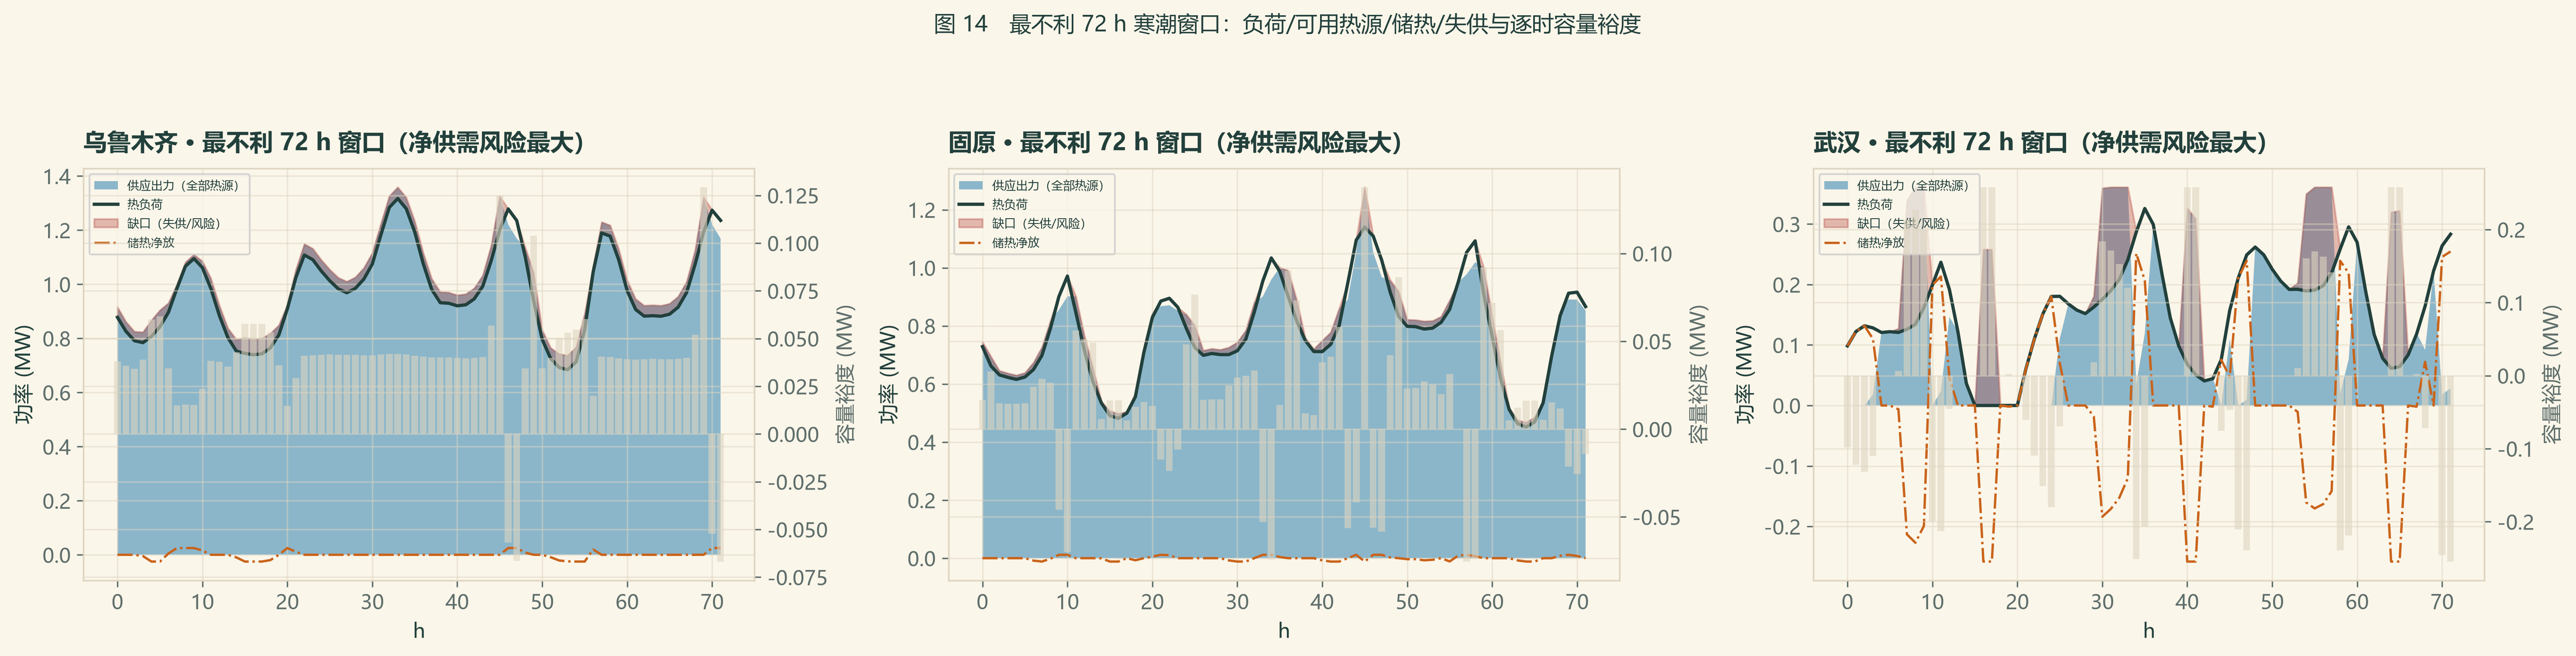
\includegraphics[width=0.98\textwidth,height=0.43\textheight,keepaspectratio,trim=0 0 0 100,clip]{media/code-results/fig14_worst_72h_resilience.png}
\caption{最不利72 h韧性窗口}
\label{fig:code-worst72}
\end{figure}

与“单年或五年聚合代表时段、最小化平均成本”的基准相比，多气象年回放使用约3---4倍代表行数，5个气象年的容量审计均通过，最差场景失供率仍为0。消融实验、压力测试和数据可靠性分级见图\ref{fig:alg-ablation}。

\begin{figure}[H]
\centering
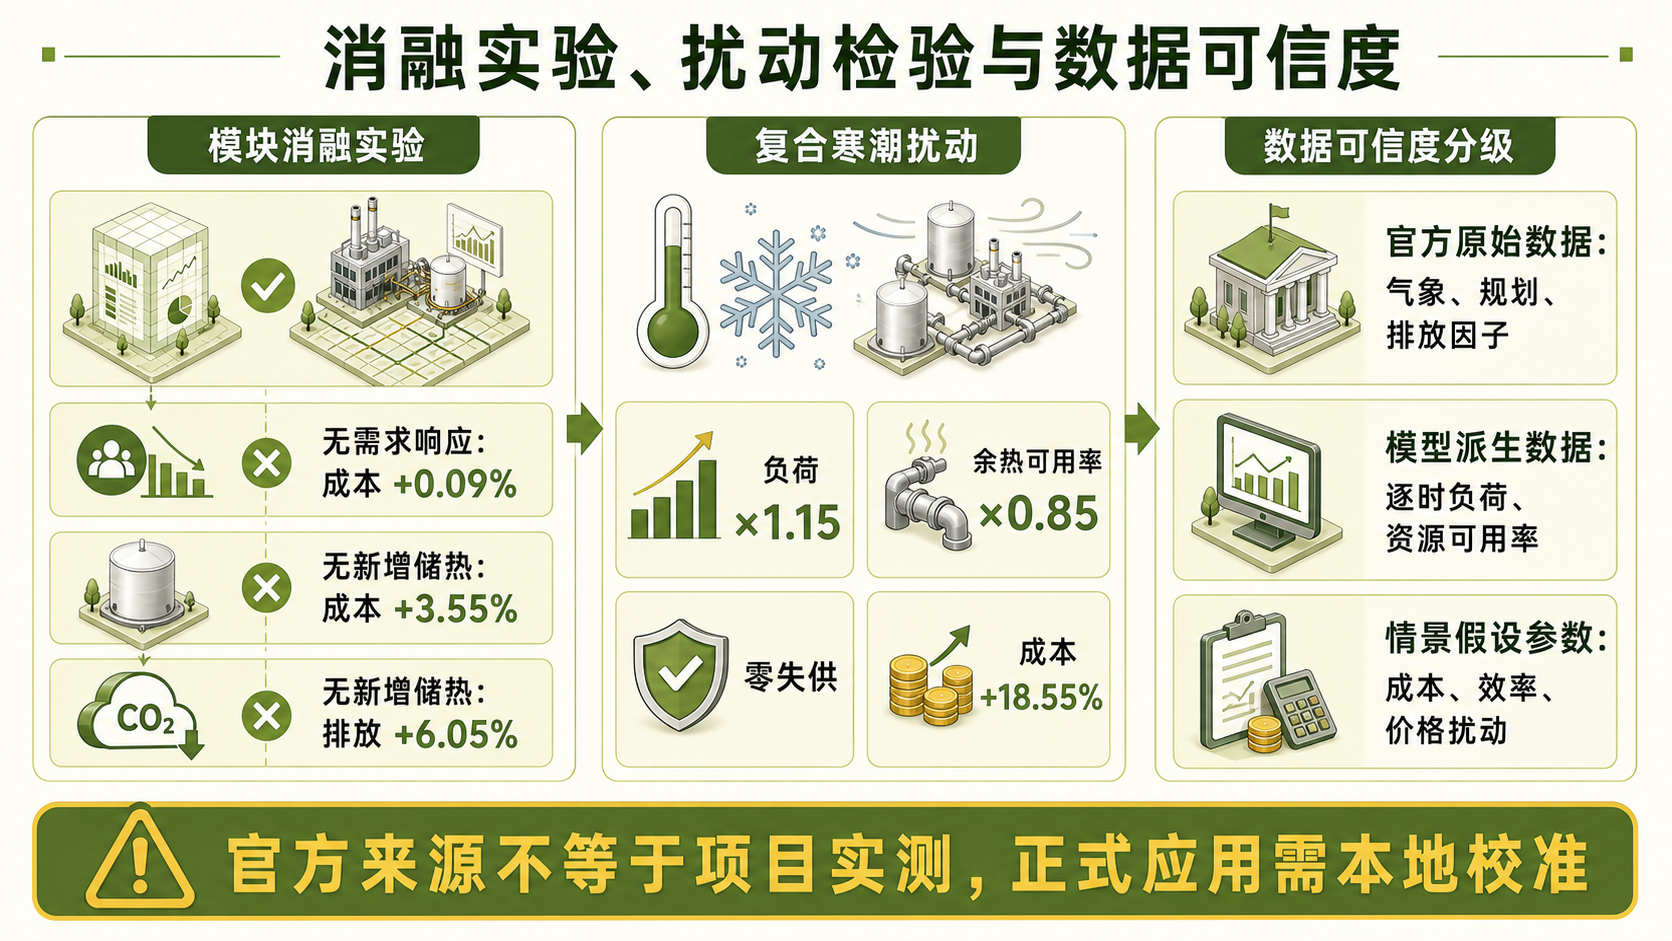
\includegraphics[width=0.76\textwidth,height=0.30\textheight,keepaspectratio]{media/algorithm-revision/fig5.png}
\caption{消融实验、扰动检验与数据可靠性}
\label{fig:alg-ablation}
\end{figure}

\subsection{数据基础与适用范围}

气象数据采用NASA POWER格点逐时数据，空间分辨率为$0.5^{\circ}\times0.625^{\circ}$，不作为地面站实测数据。标准、批复与政府文件为适用字段提供来源；派生负荷、原型热工和容量、设备成本与燃料价格按历史算例假设登记。数据记录包括来源、链接、检索时间、单位、分辨率、换算公式和适用局限。

碳排放统一采用2023年全国电力平均排放因子0.5306~kg~CO$_2$/kWh计算。新疆、宁夏和湖北的省级参考因子分别为0.6021、0.6187和0.4044~kg~CO$_2$/kWh，省级因子重算可作为地方应用时的补充。三场景均为代表性多节点系统，缩比系数仅用于规模换算，不表示对城市地理系统的完整复刻，横向比较采用单位指标。

\subsection{小结}

算法采用$\varepsilon$-约束处理成本与碳排放的多目标关系，以硬边界约束可靠性，并以$\lambda$-CVaR描述风险态度。乌鲁木齐获得投资---运行联合解；固原和武汉获得锚定投资模式下的全季运行解。三场景热平衡最大绝对残差分别为$7.41\times10^{-13}$、$1.25\times10^{-10}$和$8.53\times10^{-14}$~kW。多尺度耦合通过节点---温位聚合、建筑等效热状态递推以及城市、区域与用户层之间的共享变量实现。

原稿报告成本---碳排放二维$\varepsilon$-约束登记候选解；非支配性限于已取得且口径一致的样本。后续可进一步开展三维Pareto扩展、省级排放因子重算，以及连续温位、C\&CG、Benders分解和在线MPC等方法的计算研究。


\clearpage
\section{数据体系与模型验证}\label{minor:data}

本章记录输入数据来源、参数处理方法、验证结果和交付文件。来源审核先检查字段依据和单位，数值复核再检查能量平衡与状态递推；两类记录分别保存。

图\ref{fig:model-095}依次列出数据准备、参数标定、样本外验证和工程验收四个环节，各环节的适用范围在下文说明。

\begin{figure}[H]
\centering
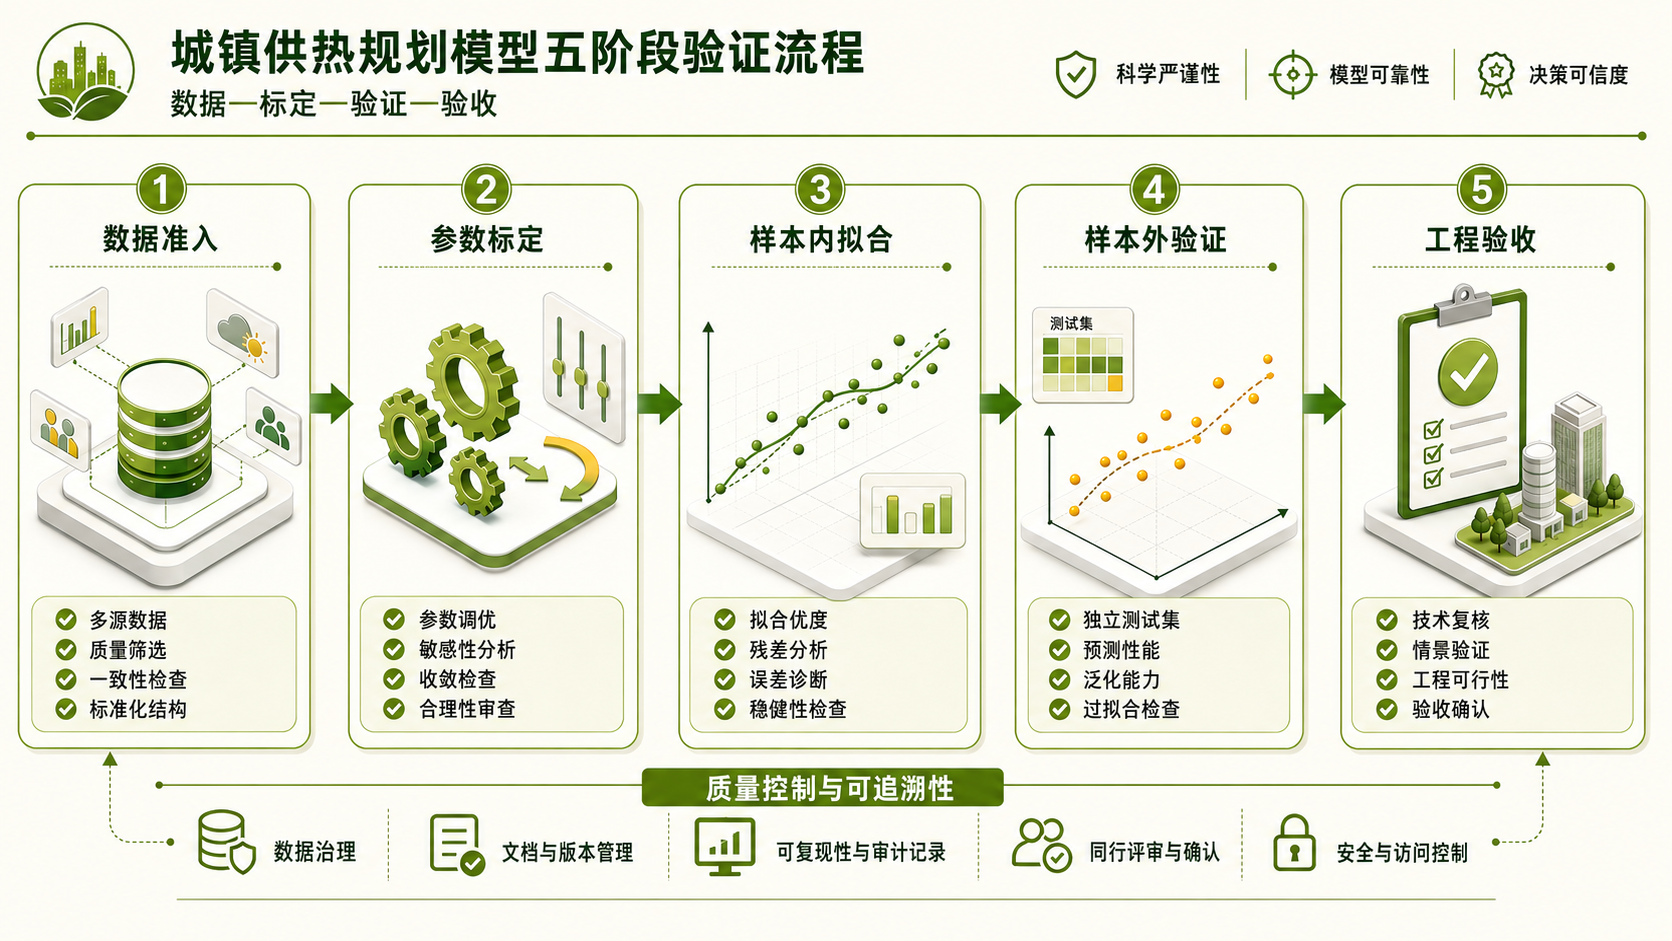
\includegraphics[width=0.714\textwidth,height=0.34\textheight,keepaspectratio]{media/model-figures/095.jpg}
\caption{数据—标定—验证—验收}
\label{fig:model-095}
\end{figure}

\subsection{场景配置矩阵}

\begin{longtable}[]{@{}p{0.07\textwidth}p{0.26\textwidth}p{0.14\textwidth}p{0.16\textwidth}p{0.17\textwidth}@{}}
\caption{模块启用与验证情况}\label{tab:20}\\
\toprule\noalign{}
\begin{minipage}[b]{\linewidth}\raggedright
场景
\end{minipage} & \begin{minipage}[b]{\linewidth}\raggedright
模块
\end{minipage} & \begin{minipage}[b]{\linewidth}\raggedright
代码支持
\end{minipage} & \begin{minipage}[b]{\linewidth}\raggedright
本次启用
\end{minipage} & \begin{minipage}[b]{\linewidth}\raggedright
结果验证
\end{minipage} \\
\midrule\noalign{}
\endfirsthead
\endhead
\bottomrule\noalign{}
\endlastfoot
C1 & 退役、余热、热泵、管网、储热 & 支持 & 启用 & 联合求解及全季校核 \\
C1 & BTES多年动态、连续水力 & 支持 & 未启用 & 未形成算例结果 \\
C2 & 给定站点与用户归属、燃料库存、微网 & 支持 & 按配置启用 & 锚定投资后全季校核 \\
C2 & 污染物、可负担性、运维可达性 & 支持 & 部分启用 & 仅报告已启用指标 \\
C3 & 给定形态、热泵、储热、配电 & 支持 & 按配置启用 & 锚定投资后全季校核 \\
C3 & 热湿、结露、噪声、地源平衡 & 支持 & 未启用 & 作为扩展模块说明 \\
\end{longtable}


\subsection{最小数据集}

\begin{longtable}[]{@{}
  >{\raggedright\arraybackslash}p{(\columnwidth - 6\tabcolsep) * \real{0.1442}}
  >{\raggedright\arraybackslash}p{(\columnwidth - 6\tabcolsep) * \real{0.1549}}
  >{\raggedright\arraybackslash}p{(\columnwidth - 6\tabcolsep) * \real{0.3237}}
  >{\raggedright\arraybackslash}p{(\columnwidth - 6\tabcolsep) * \real{0.3771}}@{}}
\caption{最小数据集}\label{tab:21}\\
\toprule\noalign{}
\begin{minipage}[b]{\linewidth}\raggedright
数据类别
\end{minipage} & \begin{minipage}[b]{\linewidth}\raggedright
建议分辨率
\end{minipage} & \begin{minipage}[b]{\linewidth}\raggedright
共用字段
\end{minipage} & \begin{minipage}[b]{\linewidth}\raggedright
场景专用字段
\end{minipage} \\
\midrule\noalign{}
\endfirsthead
\endhead
\bottomrule\noalign{}
\endlastfoot
GIS/资产 & 设备、管段、建筑级 & 坐标、道路、长度、管径、年代、地块 & C1
既有状态；C2 村镇/道路；C3 地下空间/声敏点 \\
运行监测 & 5--60 min & 热量、流量、压力、供回水温度、电功率 & C1 CHP
工况；C3 室内温湿度与启停 \\
热源资源 & 15 min--日 & 可用量、源温、检修、位置 & C1 余热停产；C2
生物质来源；C3 水源/地源许可 \\
建筑负荷 & 15 min--小时 & 面积、用途、末端、热量、室温 & C2
收入/运维；C3 占用、冷量、热水、湿度 \\
气象 & 小时 & 干球温度、风、辐照 & C3 湿球/相对湿度、结霜工况 \\
电力/碳 & 小时 & 电价、边际碳因子、变压器容量 & C2/C3
台区增容与停电影响 \\
成本/寿命 & 年度 & CAPEX、OPEX、寿命、残值、碳价 &
退役、物流、仓储、班组、声学治理 \\
\end{longtable}


\subsection{参数标定与外部验证}

参数来源按``实测监测---设备/设计资料---同行评审工程文献---合理区间假设''四级记录。能够获得的气象、负荷、资产、价格和碳因子使用目标城市数据；建筑
等效热容、管段热损、水力阻力、CHP 运行域、储热和 BTES
参数若无法实测，则采用公开工程参数作为中心值，并设置上下限开展敏感性分析。SSRN
预印本\supcite{3}用于补充相关技术信息；温位匹配、低温网和 BTES
的关键参数依据目标项目数据、工程资料或同行评审文献确定，不采用文献单点值作为全国统一参数。

有足够数据时，使用未参与参数辨识的年份或天气序列做样本外验证；数据不足时，至少保留一个寒潮连续时段和一个过渡期时段，并公开参数区间。三个场景均采用统一的守恒、求解和验收接口完成连续供暖季计算；各场景的输入来源与适用范围分别说明，代理数据与现场实测数据分别登记。

如图\ref{fig:model-096}所示，本图仅说明验证方法；样本内参数辨识与样本外气象回放分开实施，实际精度以求解日志和逐时记录为准。

\begin{figure}[H]
\centering
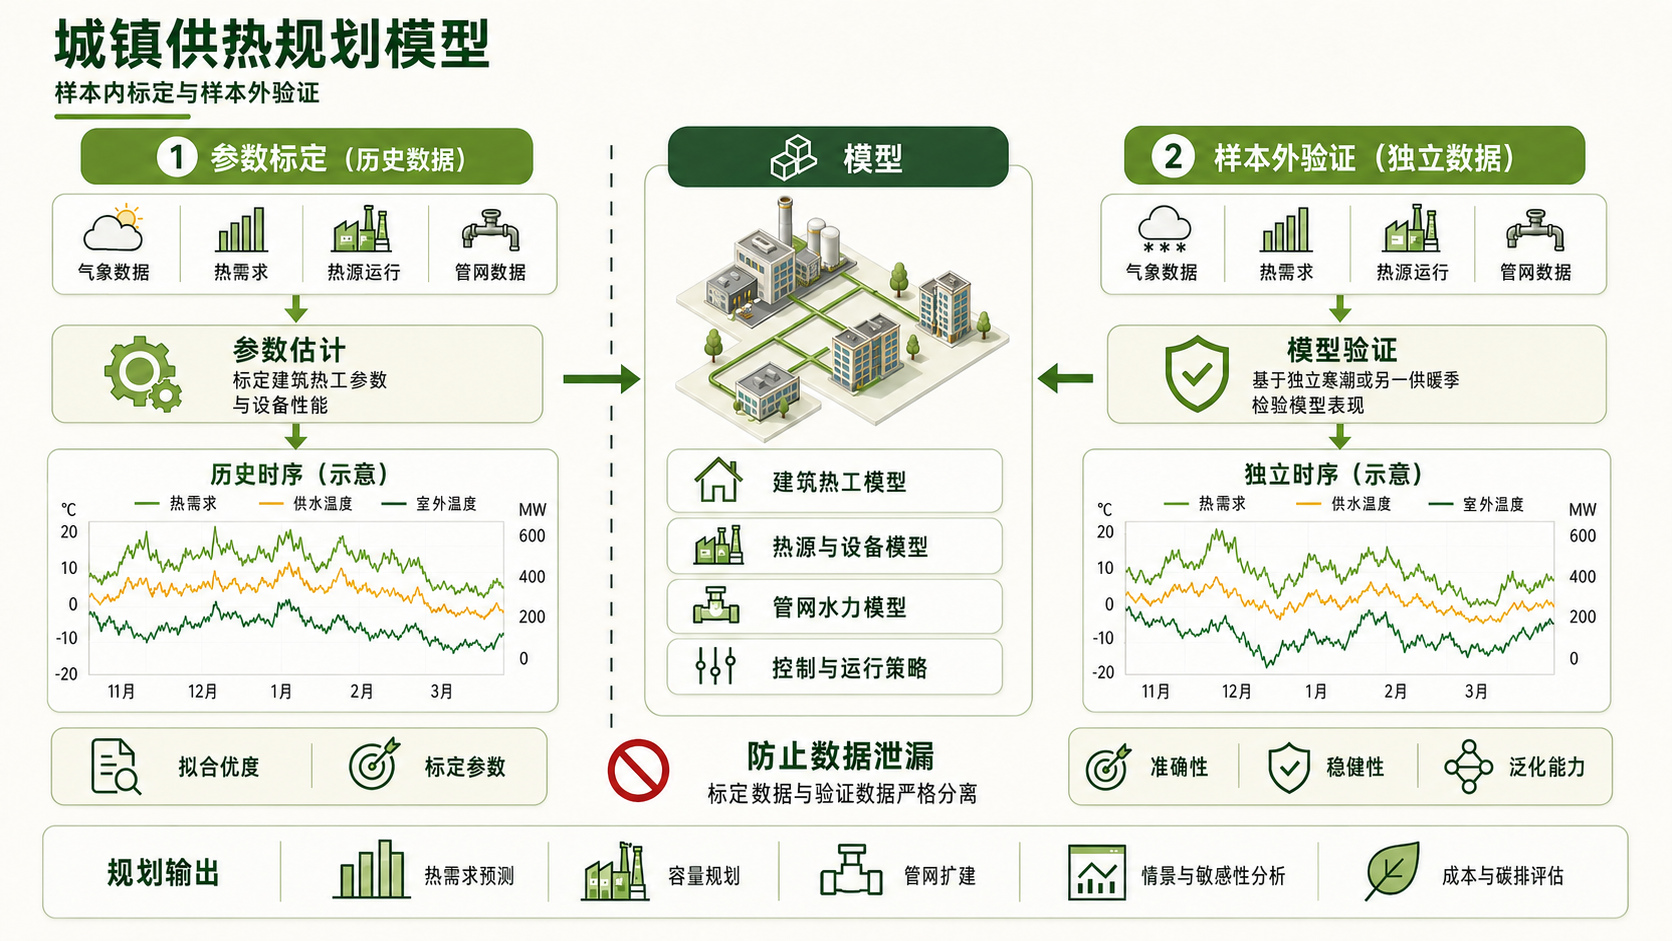
\includegraphics[width=0.714\textwidth,height=0.34\textheight,keepaspectratio]{media/model-figures/096.jpg}
\caption{样本内与样本外验证方法示意}
\label{fig:model-096}
\end{figure}

\subsection{工程验收标准}

以下列出工程验收目标。实际启用项和已完成检查以配置矩阵及对应运行记录为准。

\begin{enumerate}
\def\labelenumi{\arabic{enumi}.}
\tightlist
\item
  所有节点、载体、库存和状态方程在容差内闭合，单位和时间权重一致。
\item
  正常情景无计划外失供；已纳入测试的极端和 N−1
  情景满足应急室温、持续时间与恢复要求。
\item
  管网温度、压力、流速和泵工况通过非线性复核；对启用了启停与爬坡模块的设备，再校核最小开停时间、爬坡和部分负荷边界。
\item
  C1 的降温与末端改造同步，最大热源 N−1 通过；BTES 和关键管段 N−1
  启用时满足相应要求。
\item
  启用 C2
  对应模块时，生物质质量---热量---库存闭合，污染物达标，物流中断和微网孤岛通过，供热费用可负担。
\item
  启用 C3
  对应模块时，占用温湿度、升温时间、湿冷除霜、声环境、地源平衡与配电峰值达标。
\item
  成本、碳、资源、折现率和不确定性情景参数（或启用预算集时的\(\Gamma\)）的敏感性结论稳定，推荐方案不是单点参数偶然结果。
\item
  所有差分状态式均以 \(\Delta x/\Delta t\)
  表示变化率；孤岛、热回收、热损和储能账本不存在虚拟供给或重复计量。
\item
  政策淘汰期限、清洁供热占比、污染物总量、年度投资和供热季禁施工窗口均通过项目配置文件加载并满足。
\end{enumerate}


建筑入口热量、聚合节点等效热状态及生活热水（启用时）在时间权重下闭合。三个场景的热平衡最大绝对残差依次为$7.41\times10^{-13}$、$1.25\times10^{-10}$和$8.53\times10^{-14}$~kW，均低于$10^{-6}$~kW的数值容差。


目标温位下的节点供热、回水温度和最小供回水温差按已启用模块检查；连续水力和房间级温度属于工程扩展校核。

如图\ref{fig:model-097}所示，热量、电力、库存和状态方程的残差均需控制在统一数值容差以内。

\begin{figure}[H]
\centering
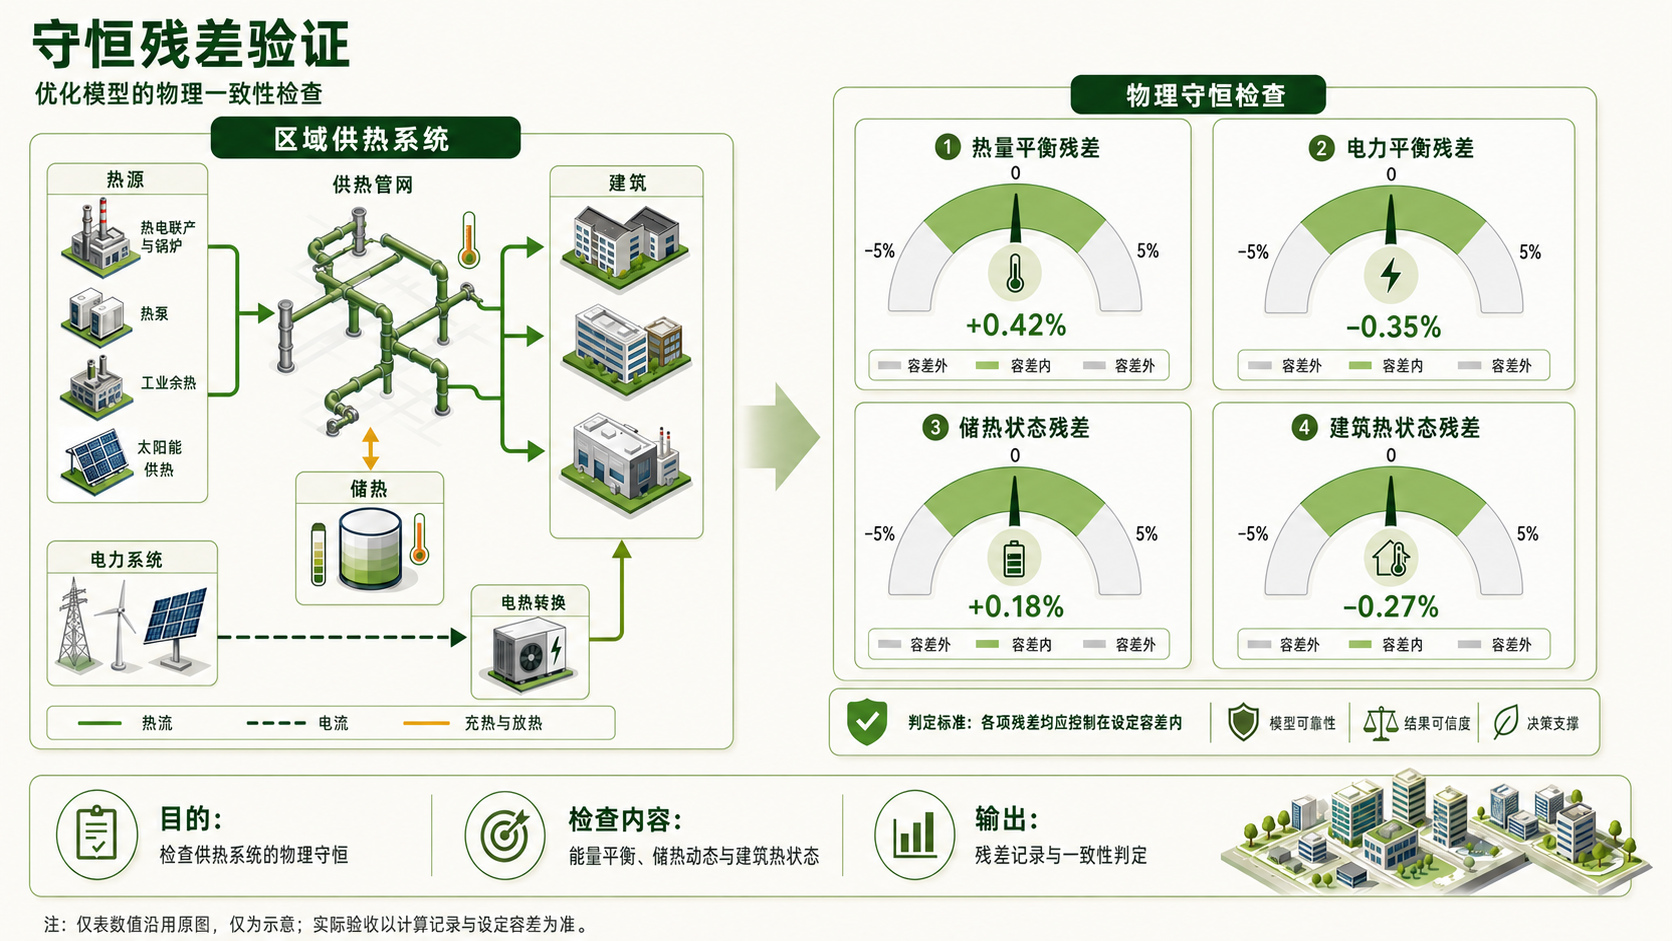
\includegraphics[width=0.714\textwidth,height=0.34\textheight,keepaspectratio]{media/model-figures/097.jpg}
\caption{守恒残差验证}
\label{fig:model-097}
\end{figure}

需求响应不超过计量控制覆盖和参与率，并在退出或同步恢复情景下仍可运行。


三个场景均给出完整供暖季数值结果，并统一报告规划求解、连续时序回放、压力测试和机器验收结果；仅在连续水力、声学、地源等专业复核模块上说明实际启用范围。

如图\ref{fig:model-098}所示，最大流量管段、最远换热站和最不利建筑是工程复核的重点断面。

\begin{figure}[H]
\centering
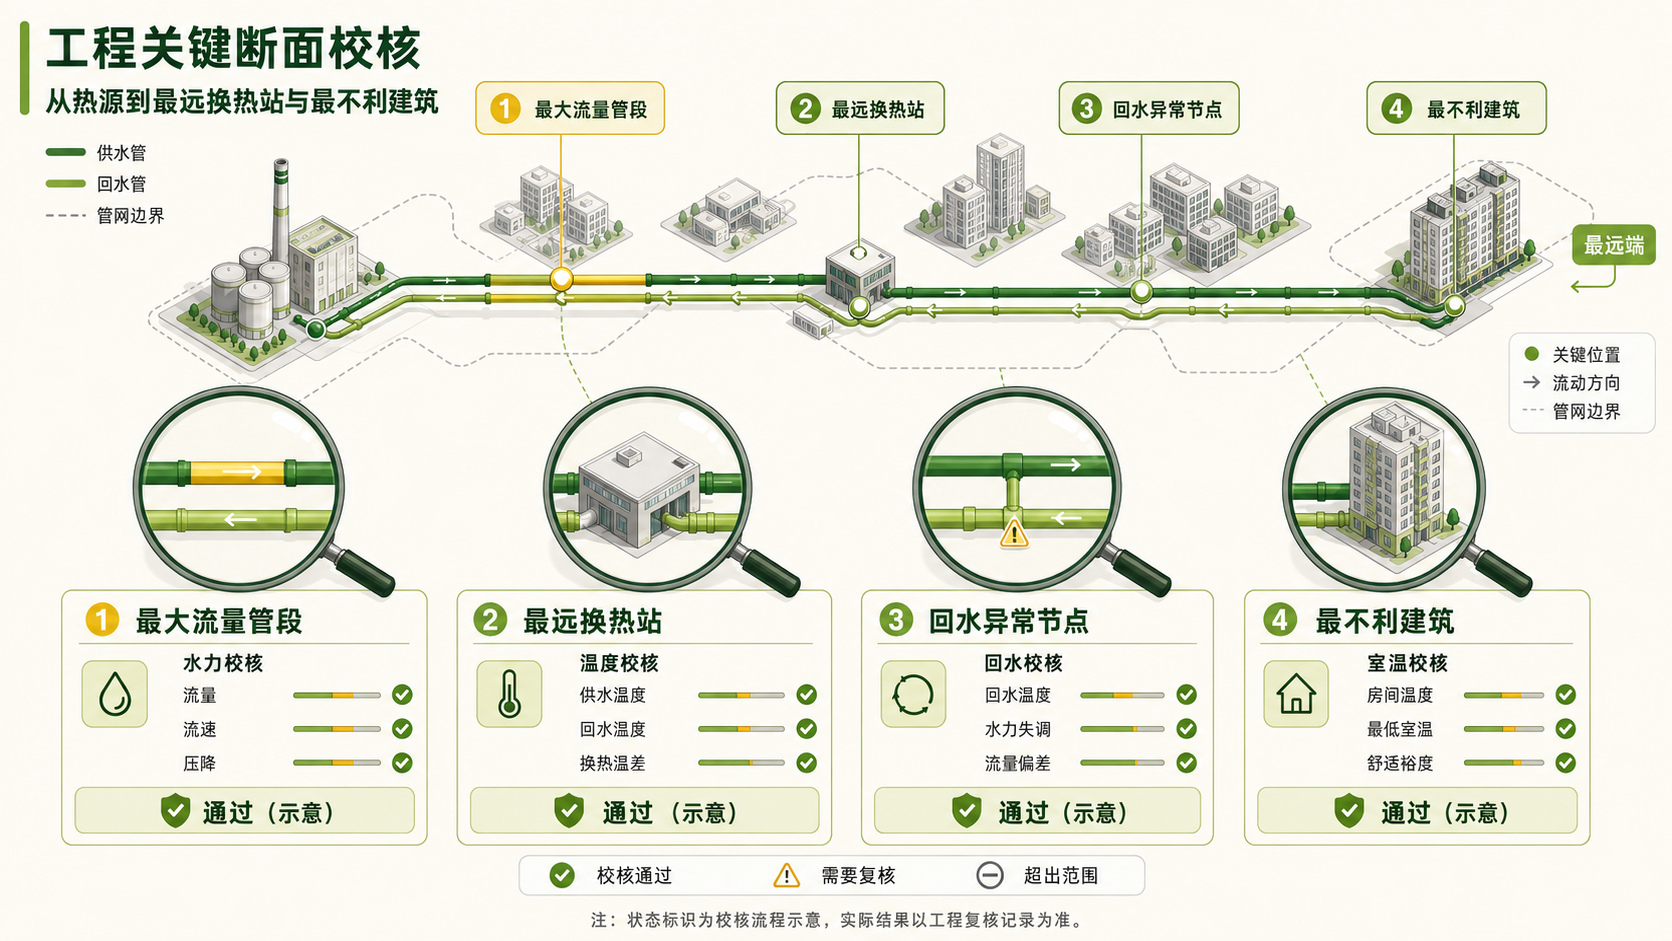
\includegraphics[width=0.714\textwidth,height=0.34\textheight,keepaspectratio]{media/model-figures/098.jpg}
\caption{工程关键断面校核}
\label{fig:model-098}
\end{figure}

\subsection{对照与消融分析}

本次对照分析采用V4全年算例及其原有时间权重。每移除一个模块，均重新求解投资与运行变量，而非只在既定方案上删除相应成本项。已完成的对照包括去除需求响应、去除新增储热和去除火用失配惩罚；另对三个场景开展电价、负荷、碳价和资源可用率敏感性分析，并在冻结投资后完成复合寒潮测试。未实际求解的对照不作为结果报告。

完整模型年化目标为95.620万元。去除新增储热后，年化成本增加3.55\%，碳排放增加6.05\%；复合寒潮下能源运行费由50.057万元增至100.349万元，增加100.47\%，同时保持零失供。该组V4结果与三城市供暖季推荐方案分开解释，不进行跨口径直接比较。

如图\ref{fig:model-099}所示，主模型联立设备容量、节点热平衡、储热和聚合热状态；连续水力等高精度局部问题作为工程扩展，按场景列示启用范围。

\begin{figure}[H]
\centering
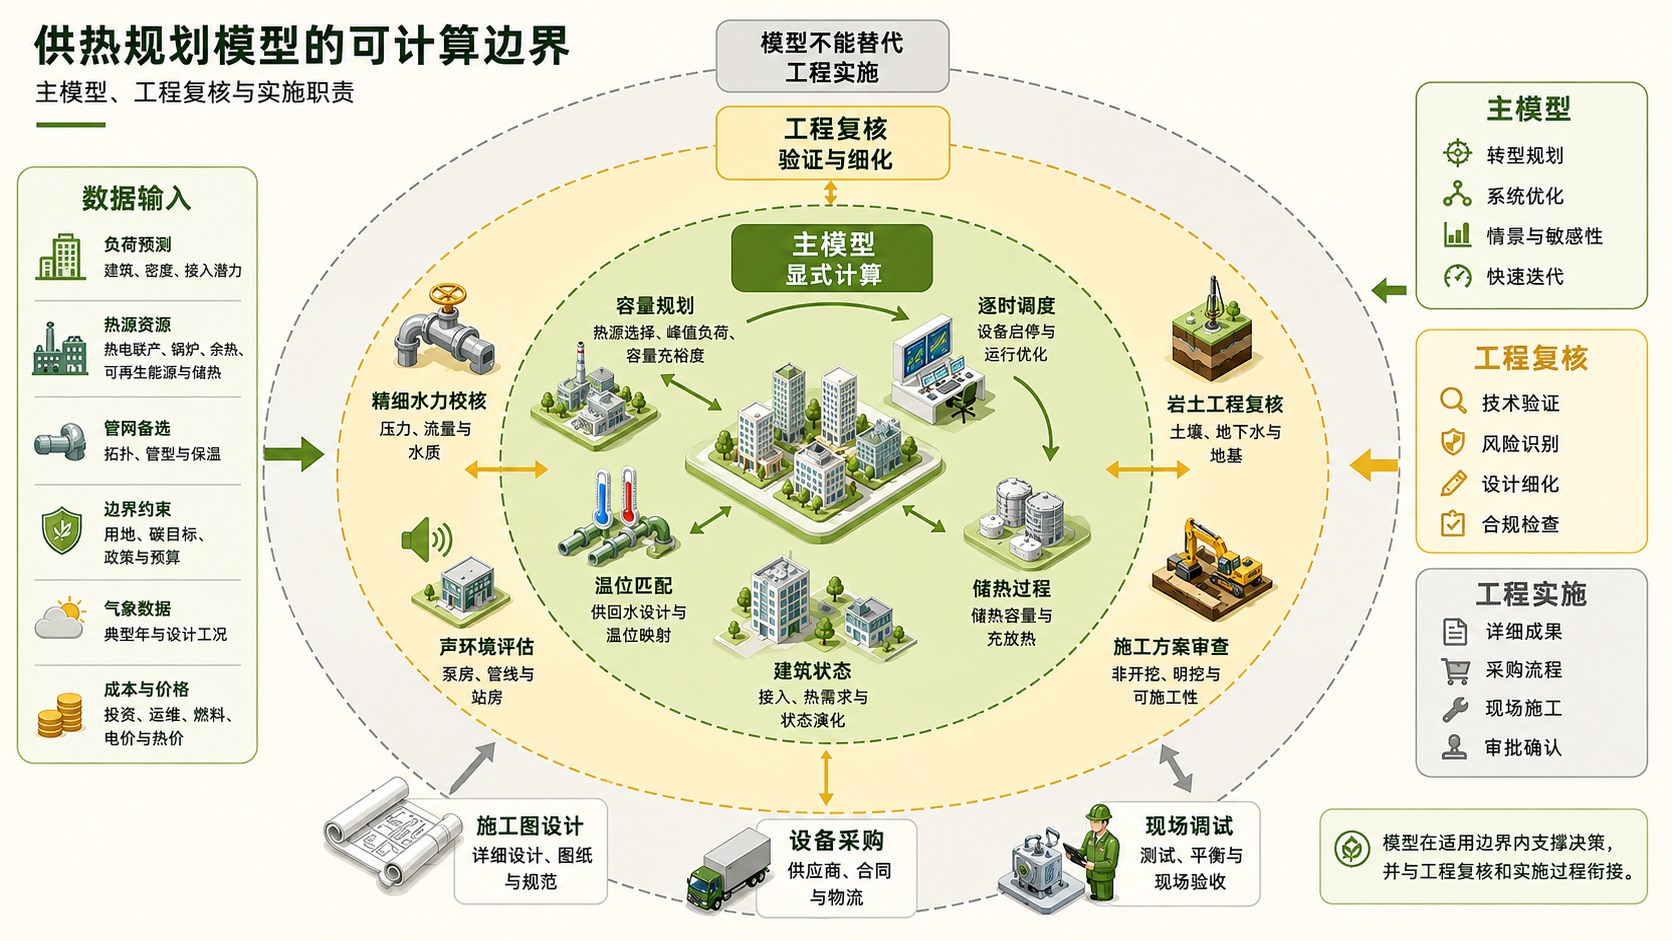
\includegraphics[width=0.714\textwidth,height=0.34\textheight,keepaspectratio]{media/model-figures/099.jpg}
\caption{可计算边界}
\label{fig:model-099}
\end{figure}

\subsection{标准化成果}

统一输出包括：数据字典与参数来源、候选链/拓扑清单、三个场景的容量配置、完整供暖季逐时调度、场景专用指标、压力测试、敏感性和校核记录。交付包根目录提供\texttt{README.md}，说明目录结构、Python依赖、Windows运行命令、三场景配置位置和供暖季输入位置；批量入口使用当前解释器调用，避免写死Python安装路径。已有结果可通过求解日志、逐时输出和验收记录交叉检查。


\subsection{结果可视化与后处理}

图表统一配色、字体和单位，展示负荷、设备出力、储热状态、成本---碳排候选解及压力情景结果。室温、回水和压力按对应实验范围报告。若分析节点边际热价，需固定整数方案后重新求解连续问题，使用节点平衡约束的对偶值；本节不以此替代已给出的成本比较。图表与场景、时段、单位和同源数据一并保存。


图\ref{fig:r8p-spatial-a3}将道路搜索结果与真实建筑、水体及用地对应，以共线路径数识别可共用的候选输配走廊。三城各取6个参考建筑节点，分别得到5、2、5条连通路径；供热能力与逐时出力仍由对应案例的设备及能量约束确定。

\begin{figure}[htbp]
\centering
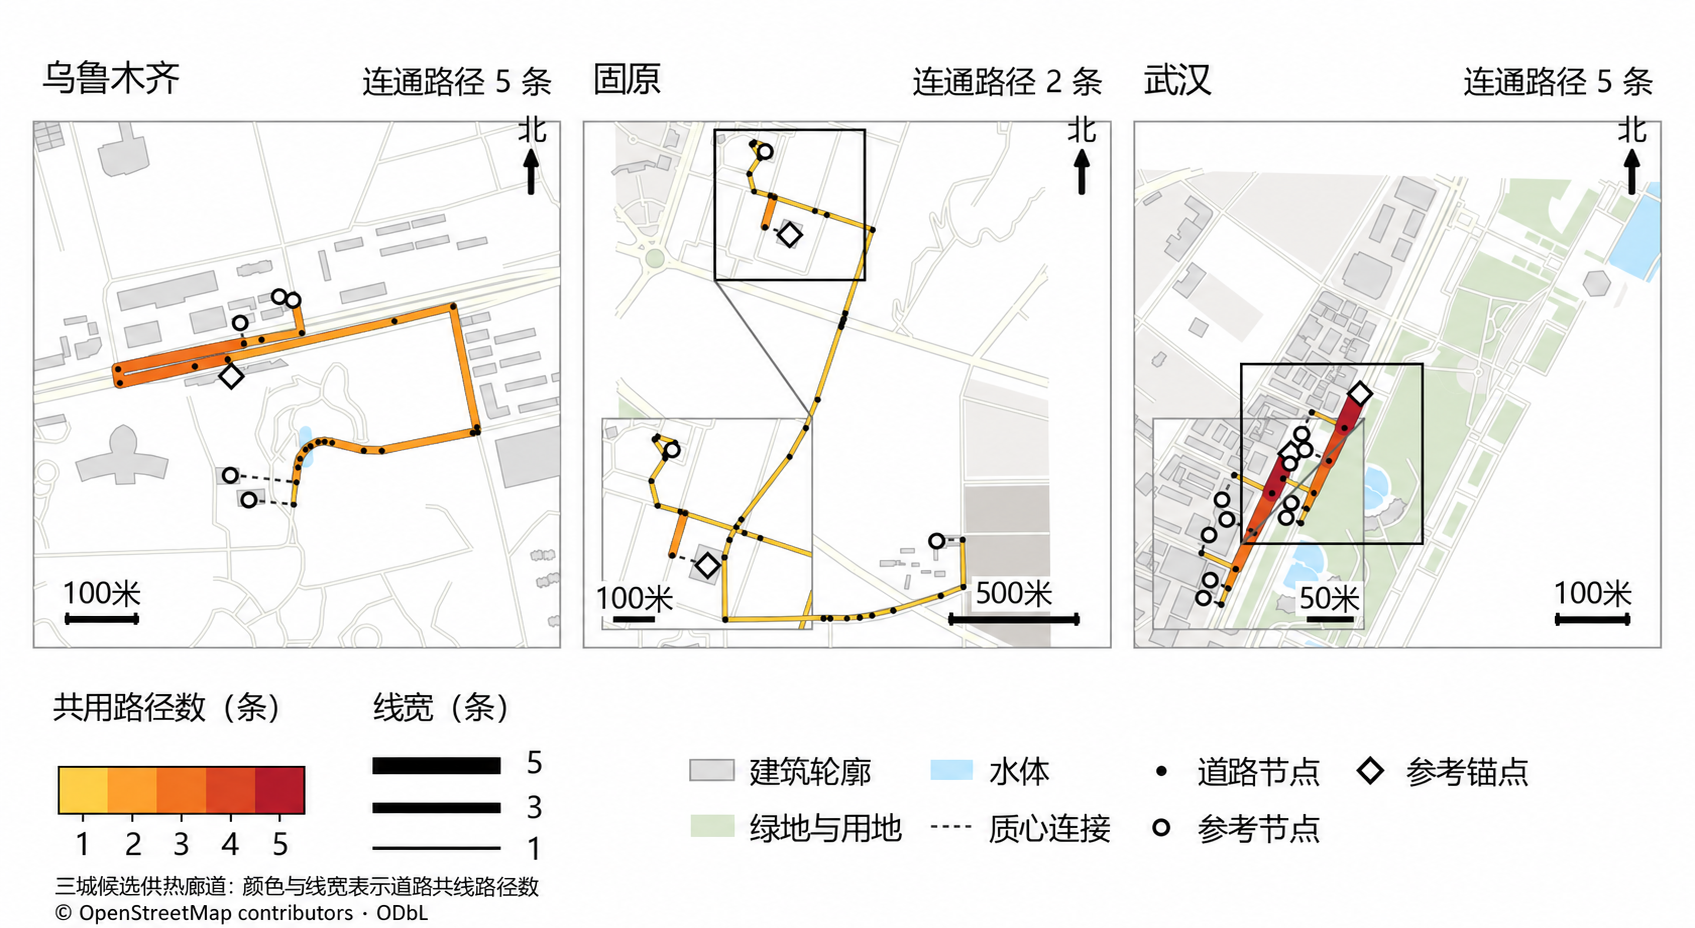
\includegraphics[width=\linewidth]{results-a3/spatial_corridors_a3.png}
\caption[三城真实地图上的候选输配廊道]{三城真实地图上的候选输配廊道。底图依据OpenStreetMap记录示意重绘；颜色与线宽表示共用路径条数，菱形为参考锚点而非热源。图示为候选连接，非已建热网或实测热流；精确几何及固原3条拒绝路径记录见随附数据。}
\label{fig:r8p-spatial-a3}
\end{figure}

% !TeX root = ../main.tex
\subsection{现有实现的补充验证}\label{minor:supplement}
以下两组对照分别检验代表日压缩与建筑热状态耦合，比较条件与结果见表\ref{tab:r8p-comparisons}。

\textbf{真实负荷的权重对照。}E01预先冻结开发集外6栋BDG2计量建筑\supcite{29}，涵盖热水、蒸汽、冷水，每栋取2017年，以同一组8--10个实际代表日比较频数、软能量校准与硬能量最小$W_1$权重。标准线性规划同时约束总日数、完整日能量与极端日权重下界，归一$W_1$中位数由软校准的12.3150\%降至4.4775\%。六例线性规划均成功，但完整统计准入仅由3/6增至4/6；两例因原观测峰被完整日筛选丢失而拒绝，回退也未达标。筛选排除了4.59\%--34.79\%的已观测能量，改善只对保留完整日成立，不能据此认定规划或运行可用。

\begin{table}[H]
\centering
\caption{两组代表性对照的完整比较口径}\label{tab:r8p-comparisons}
\begin{tabularx}{\linewidth}{@{}Yrr@{}}
\toprule
\multicolumn{3}{@{}l}{E01：同六栋建筑、同一实际日集合}\\
权重方法 & 归一$W_1$中位数/\% & 统计准入/6\\\midrule
极端日频数 & 15.4450 & 0\\
软能量校准 & 12.3150 & 3\\
硬能量最小$W_1$ & 4.4775 & 4\\
\bottomrule
\end{tabularx}
\par\vspace{4pt}
\begin{tabularx}{\linewidth}{@{}Yrrrr@{}}
\toprule
\multicolumn{5}{@{}l}{E03：双楼2880小时，热容倍率与公用电上限$2\times2$}\\
$C_B$倍率/电上限 & 电量费/元 & 电量/kWh & CO$_2$/kg & 峰值/kW\\\midrule
1/无 & 5918.14 & 8155.11 & 3297.93 & 14.1064\\
4/无 & 5490.94 & 8725.44 & 3528.57 & 25.3335\\
1/有 & 5937.64 & 8050.61 & 3255.67 & 6.4796\\
4/有 & 5660.96 & 8386.07 & 3391.33 & 6.4796\\
\bottomrule
\end{tabularx}
\end{table}

\begin{figure}[htbp]
\centering
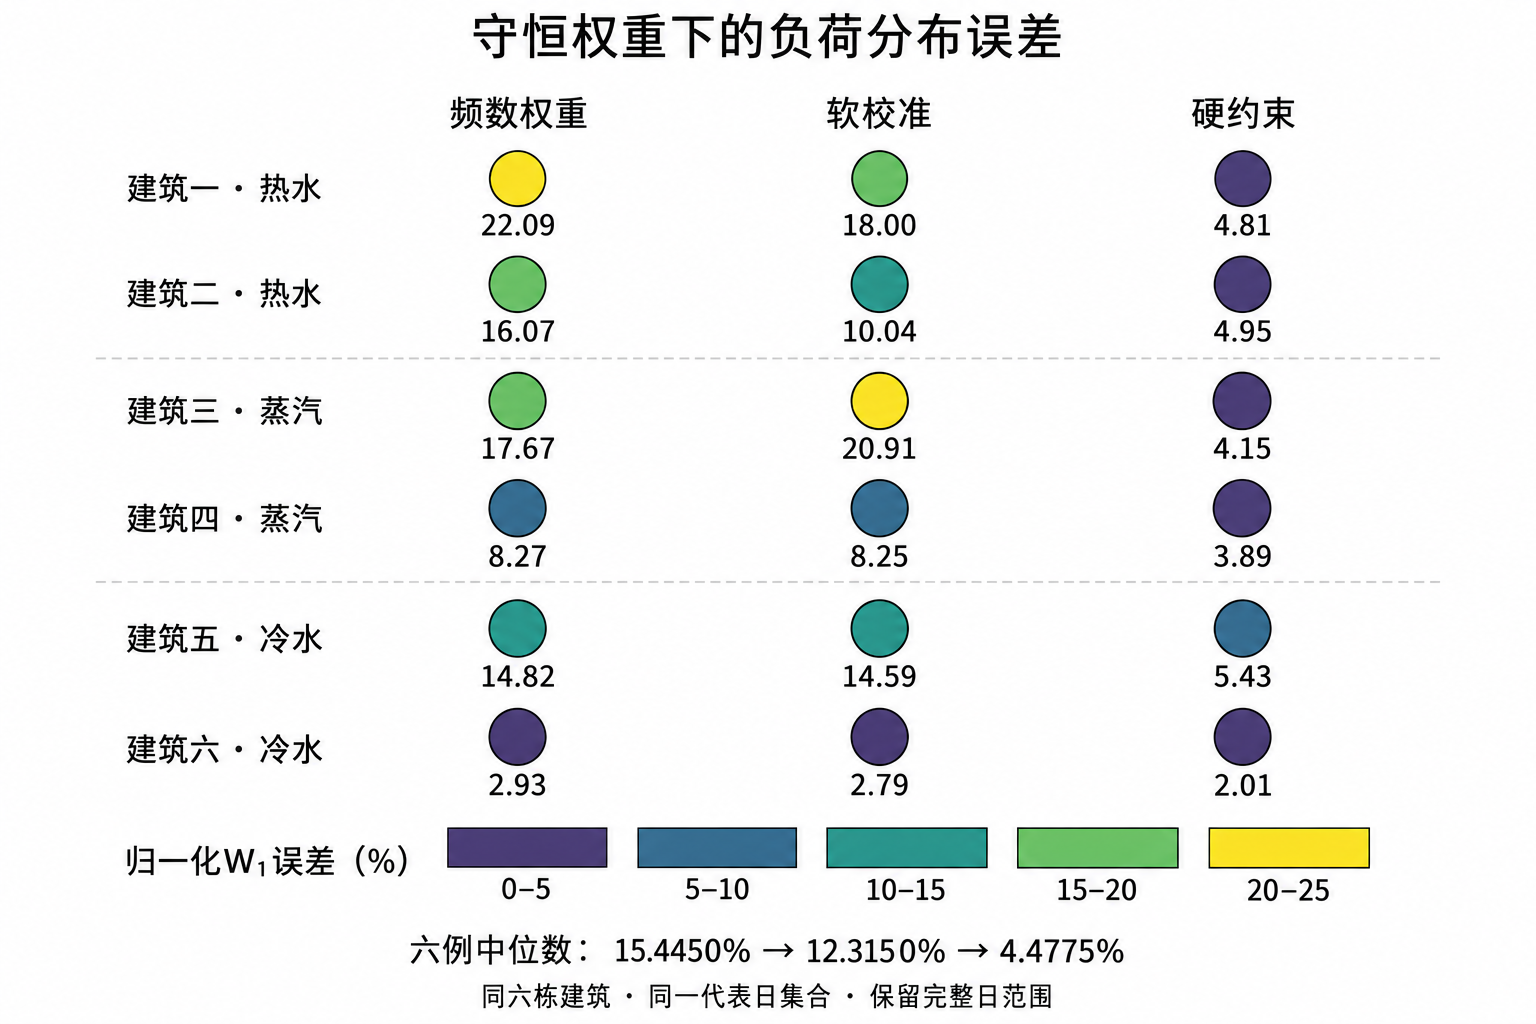
\includegraphics[width=0.93\linewidth]{results-a3/bdg2_data_a3.png}
\caption[同一代表日集合下的六楼负荷分布误差]{同一代表日集合下的六楼负荷分布误差。圆点颜色按归一$W_1$误差分箱，数值单位为\%；区间左闭右开，末档包含25。建筑一至六依次对应附录5.1的Alissa、Ian、Brandon、Genoveva、Angela、Dorethea；统计采用结果另见完整分母表。}
\label{fig:r8p-bdg2-a3}
\end{figure}

\textbf{热容与配电边界的耦合。}E03保持同一武汉公开格点天气\supcite{31}、热损系数、得热、理想设备及20--27~$^\circ$C服务，仅改变B楼热容倍率和公用电上限，连续继承2880小时状态并恢复初末20~$^\circ$C。无电上限时，四倍热容使电量费降低427.20元，却增加570.33~kWh用电；加上6.4796~kW公用上限后，省费缩为276.68元，用电仍增加335.46~kWh，费用交互为150.52元。四格求解gap均为0，独立状态、热量及配电核验通过，结论限于登记模型的固定资产运行。该对照展示用户侧热惯性向系统约束传递的可检验作用，同时区分省费、削峰与节能。其余实验、失败分母及记录路径见附录5、表\ref{tab:minor-evidence}，不与原三城工程算例的收益合并。

\begin{figure}[htbp]
\centering
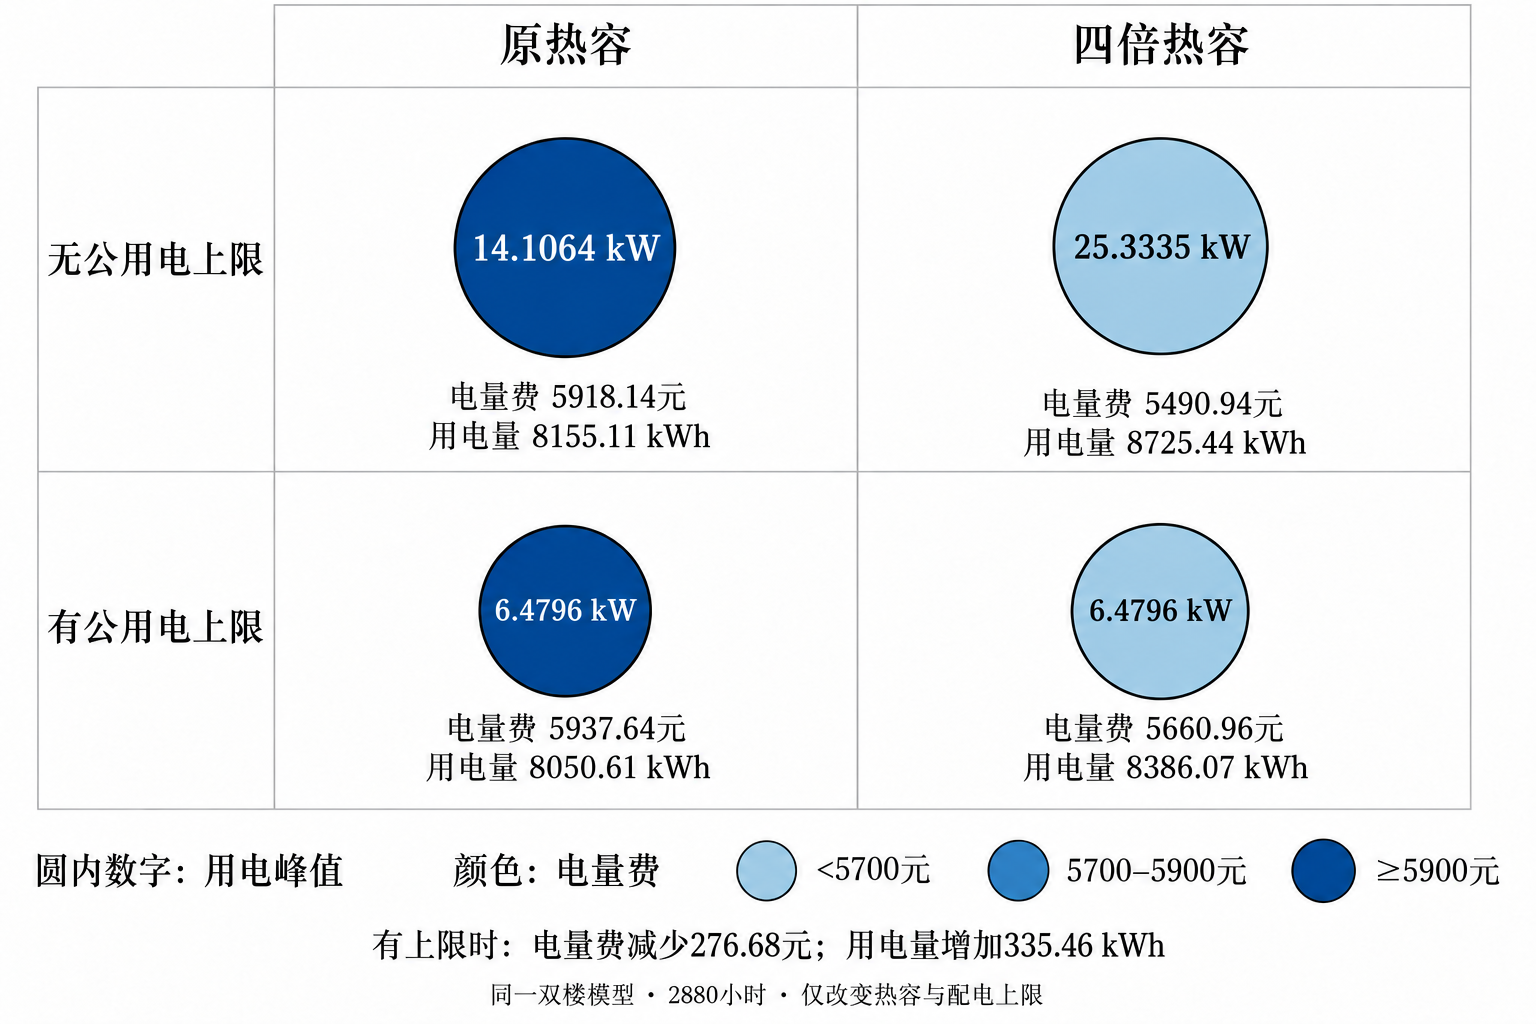
\includegraphics[width=0.95\linewidth]{results-a3/thermal_factorial_a3.png}
\caption[热容与公用电上限的四格对照]{热容与公用电上限的四格对照，仅调整B楼热容倍率。圆内标注用电峰值，颜色对应电量费区间，圆面积不作定量读数。相同配电上限下，增大热容保留移峰节费空间；电量变化与费用变化分别核算。}
\label{fig:r8p-thermal-a3}
\end{figure}

\clearpage
\section{模型应用与决策分析}\label{minor:application}

本文模型面向供热转型规划、项目比选、投资安排、风险评估和政策分析，输出容量配置、建设时序、运行指标及工程约束校核结果。

\subsection{区域供热转型规划}

模型可比较热源结构、管网温位、储热和建筑改造路径，并依据生命周期成本、碳排放、峰值化石依赖率与可靠性指标，确定各阶段资产的建设、保留、改造和退役安排。

\subsection{项目方案比选}

候选方案可在相同负荷、气象、价格和可靠性边界下比较，评价设备投资、运行费用、温位适配、配电容量、建筑舒适和故障保供，并识别容量余量与关键瓶颈。

\subsection{改造时序与投资安排}

在年度预算、施工能力和投产时间约束下，模型形成分年度建设清单，并分析项目延期对峰值容量、运行成本和备用需求的影响。

\subsection{极端情景与风险评估}

固定投资方案后，对寒潮、资源中断、价格变化、需求响应退出及关键故障进行重调度，检查失供、室温、配电峰值和储热状态，确定备用容量和应急运行边界。

\subsection{政策与低碳路径评估}

通过调整碳约束、清洁热比例、补贴、能源价格和可靠性门槛，可生成成本---减排Pareto候选集。政策判断仍需结合地方财政、资源条件和居民可负担性。

\subsection{应用流程与成果输出}

应用流程包括数据整理、候选方案求解、压力测试和工程校核。成果用于规划决策，不能替代施工图、水力平衡、设备选型、地质勘察和现场调试。

\clearpage
\section{模型创新、局限与结论}\label{minor:conclusion}

\subsection{模型创新}

\textbf{核心创新一：温位、候选管网与容量协同。}将温位兼容、候选管段容量和热源出力联立，以源温、输送上限和用户温位共同检查替代方案，避免只按供热总量配置设备。

图\ref{fig:model-125}列示热源温位、候选管段和用户需求的连接关系；本次计算采用给定温位与已登记候选连接。

\begin{figure}[H]
\centering
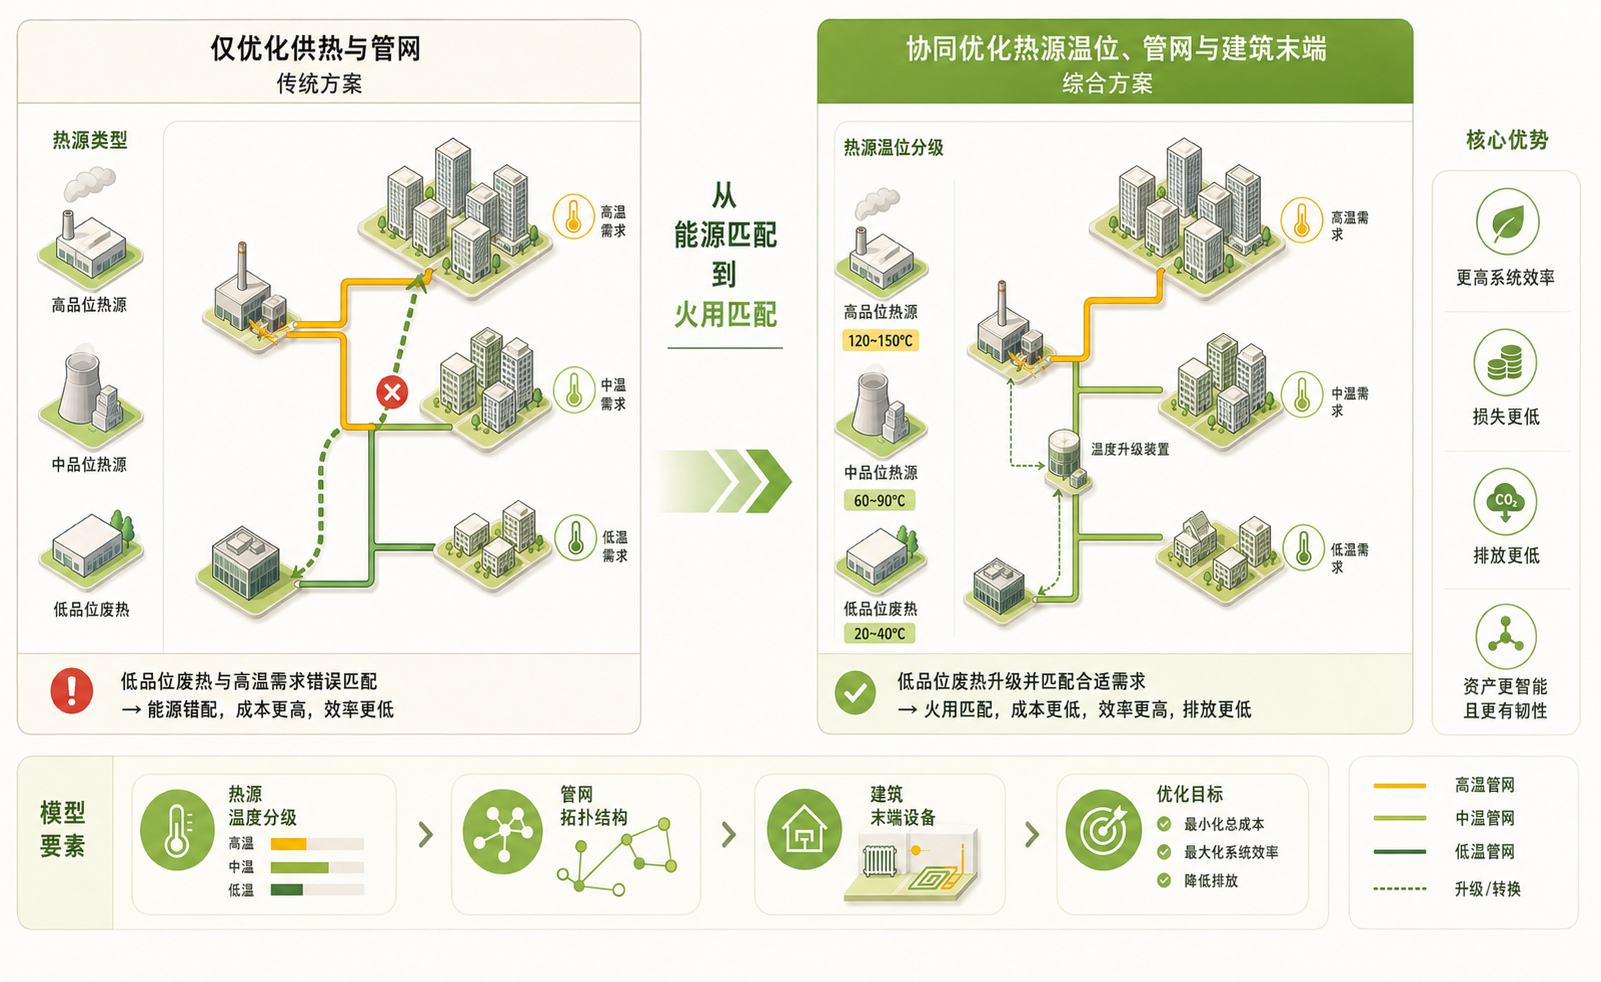
\includegraphics[width=0.714\textwidth,height=0.34\textheight,keepaspectratio]{media/model-figures/125.jpg}
\caption{创新点一：温位与候选管网协同规划}
\label{fig:model-125}
\end{figure}

\textbf{核心创新二：存量网络与改造方案共同评价。}以既有管段容量为起点，将候选管径和改造投资纳入方案比较，保留存量资产对新增热源接入的约束。

图\ref{fig:model-126}中的三态对应规划框架；本次启用的选择由管段容量、候选管径和改造配置确定。

\begin{figure}[H]
\centering
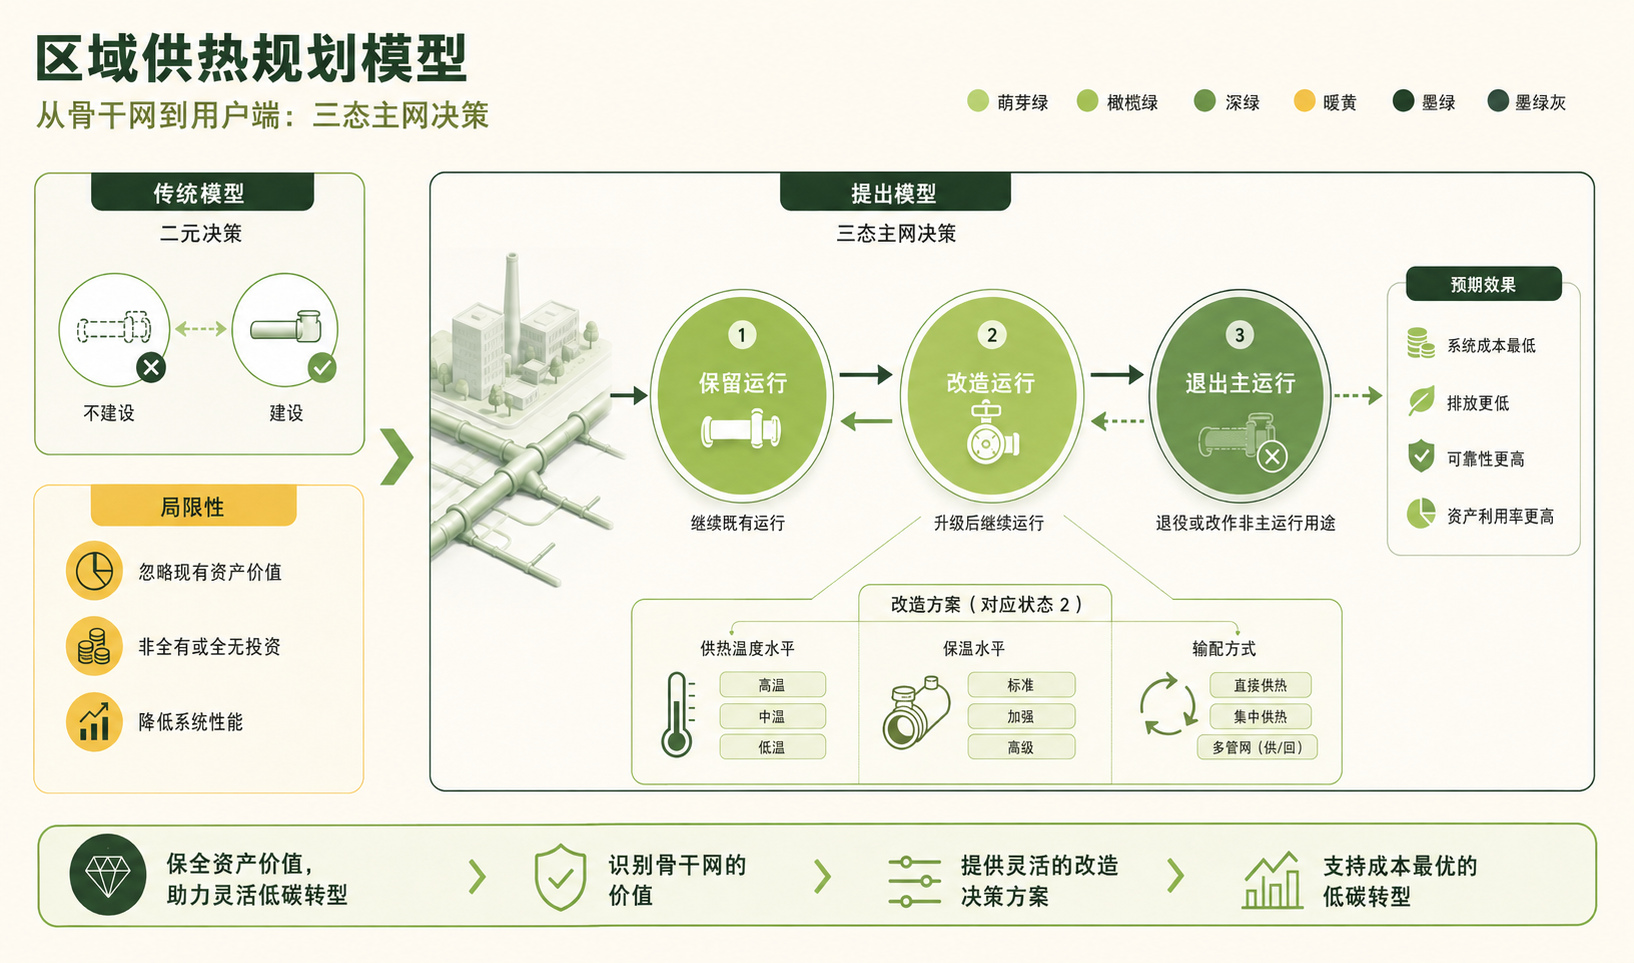
\includegraphics[width=0.714\textwidth,height=0.34\textheight,keepaspectratio]{media/model-figures/126.jpg}
\caption{创新点二：管网三态规划接口示意}
\label{fig:model-126}
\end{figure}

\textbf{核心创新三：可靠容量约束下的热源退役。}将热源退役量与替代容量共同选择，以建筑负荷、节点供热和保供边界限制退出规模；分年度时序由相应阶段配置处理。

图\ref{fig:model-127}将退役与替代容量联系起来：退出规模须满足节点供热和保供要求，再由成本目标比较可行组合。

\begin{figure}[H]
\centering
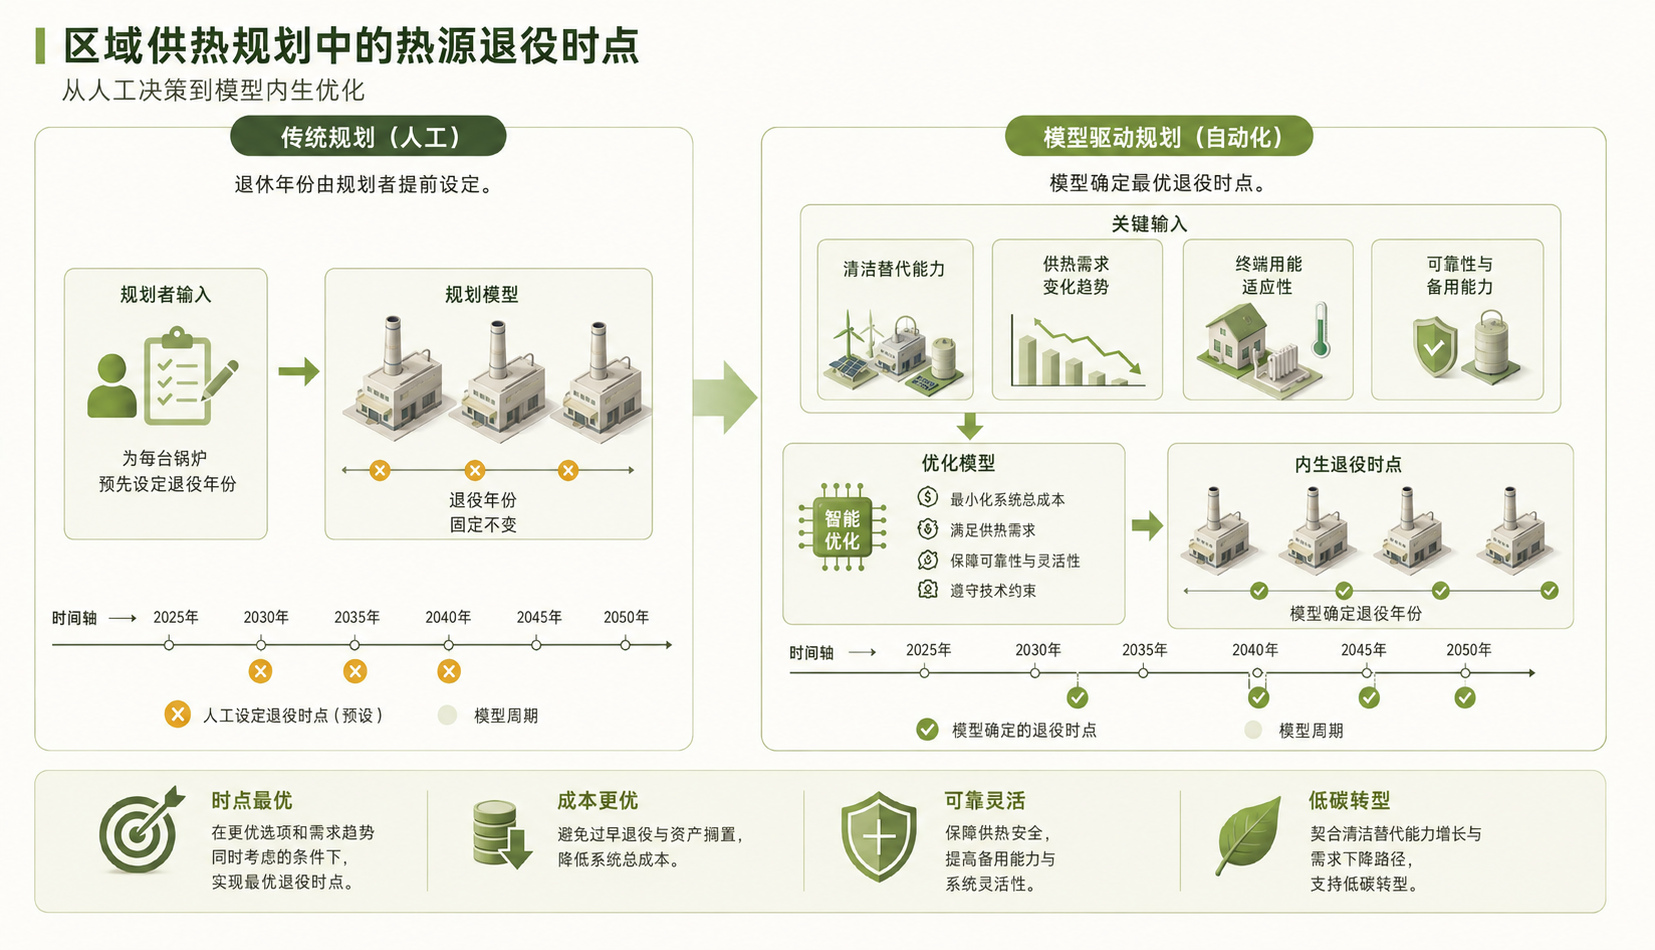
\includegraphics[width=0.714\textwidth,height=0.34\textheight,keepaspectratio]{media/model-figures/127.jpg}
\caption{创新点三：化石热源内生退役}
\label{fig:model-127}
\end{figure}
\textbf{核心创新四：建筑热状态与系统调度耦合。}将建筑热状态与热源出力、储热充放和配电约束联立，使用户侧负荷转移传递到系统调度。图\ref{fig:model-128}对应原聚合模型；独立四楼验证在8784小时服务年及2928小时冬季窗口内均无建筑状态违约，详见表\ref{tab:minor-evidence}。

\begin{figure}[H]
\centering
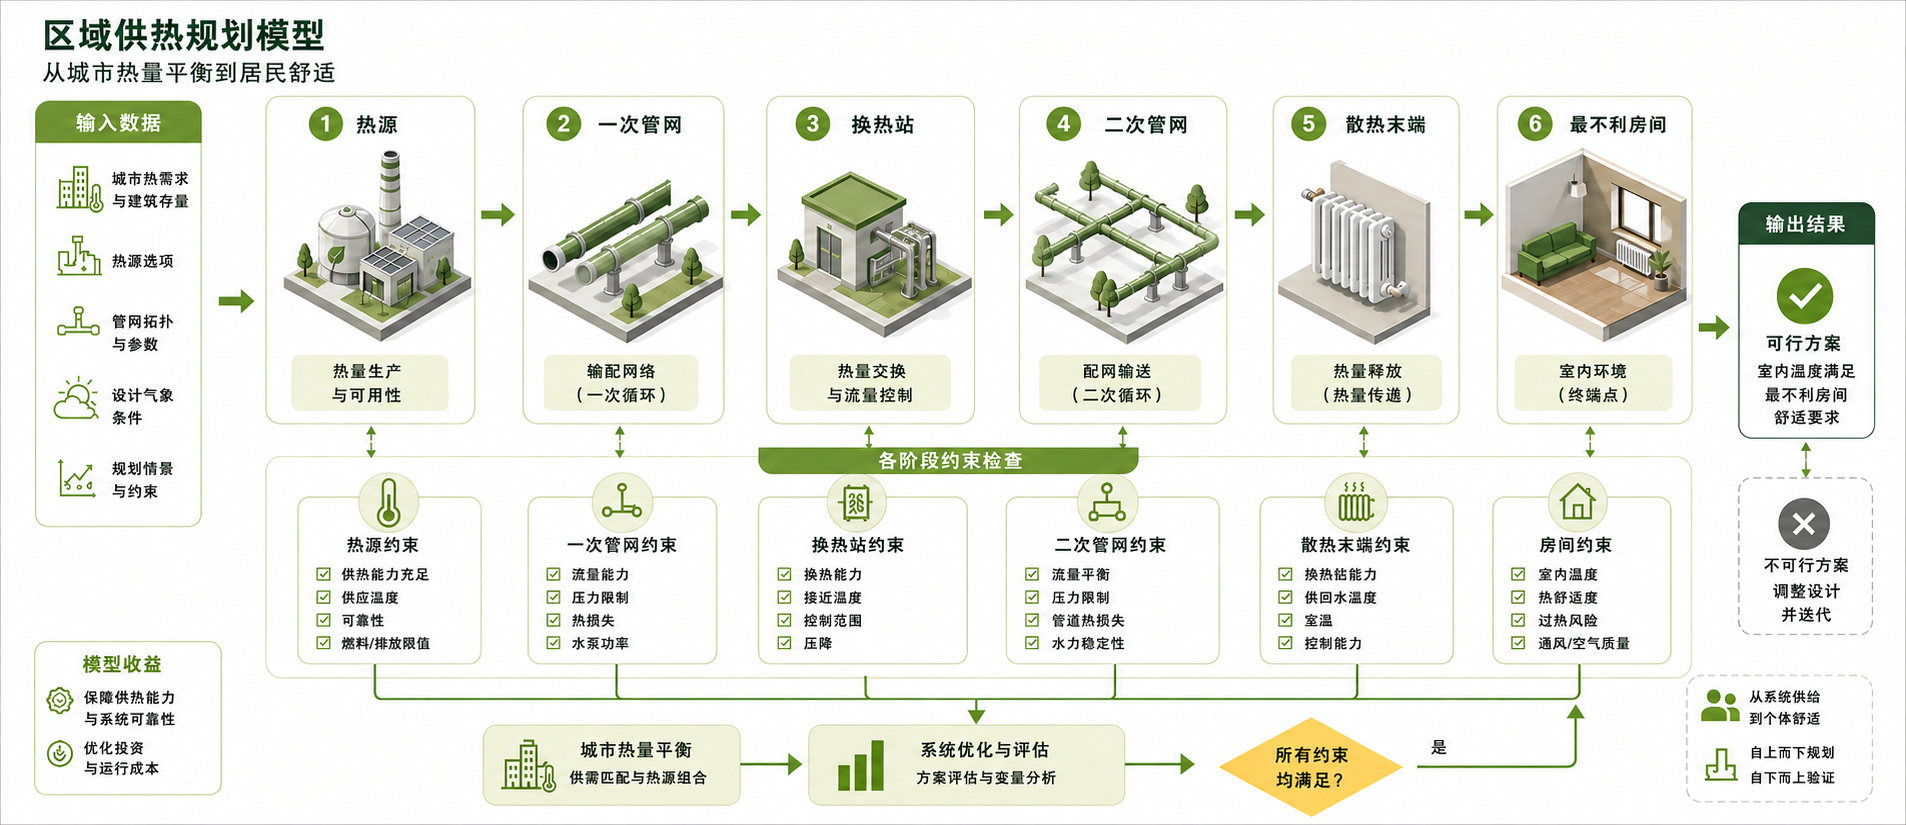
\includegraphics[width=0.714\textwidth,height=0.34\textheight,keepaspectratio]{media/model-figures/128.jpg}
\caption{创新点四：源网荷储与用户侧热惯性协同}
\label{fig:model-128}
\end{figure}

\textbf{核心创新五：规划与物理校核衔接。}图\ref{fig:model-129}表示规划与校核的连接关系。在72小时参考管网实验中，每轮排除温度或压降不合格的有限模式后重新求解，第三轮满足远端供水与压降阈值；相同交付热量下的费用变化见表\ref{tab:minor-evidence}。

\begin{figure}[H]
\centering
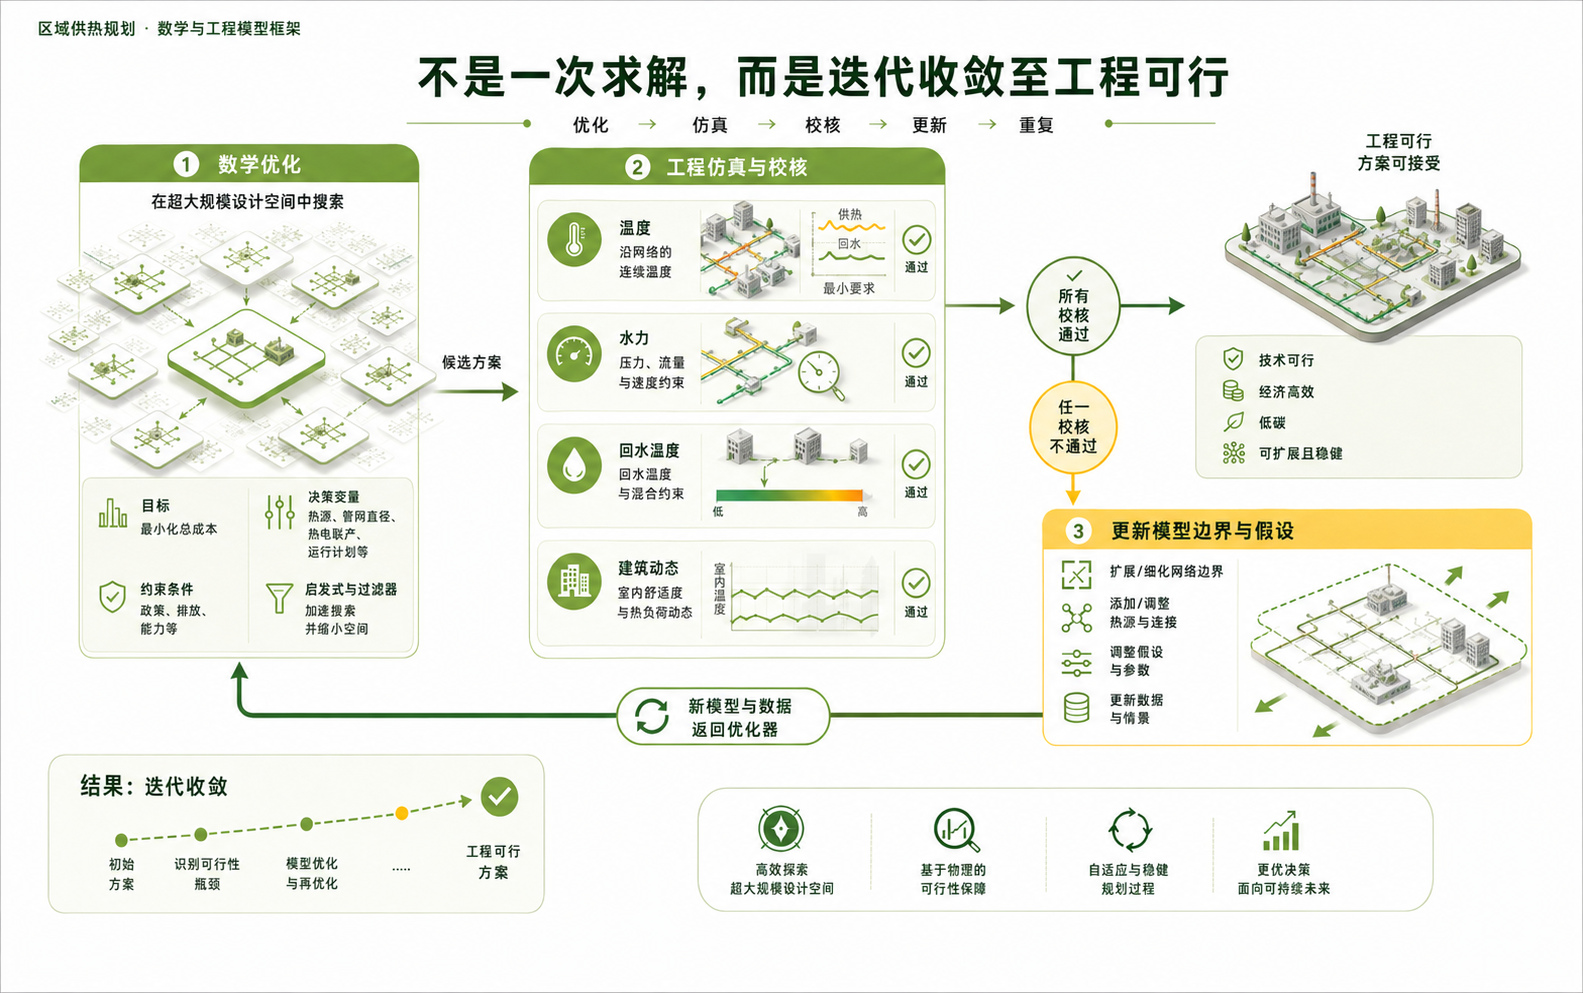
\includegraphics[width=0.714\textwidth,height=0.34\textheight,keepaspectratio]{media/model-figures/129.jpg}
\caption{创新点五：优化—校核闭环}
\label{fig:model-129}
\end{figure}

\textbf{核心创新六：公共模型与差异化场景配置。}三类场景共用负荷、节点平衡、设备容量、储热和电力约束，分别加载既有热网改造、分散资源供应与间歇供热条件。

图\ref{fig:model-130}给出共用关系与场景差异。乌鲁木齐采用投资---运行联合求解，固原、武汉采用锚定投资后的逐时运行校核，结果按各自求解范围比较。

\begin{figure}[H]
\centering
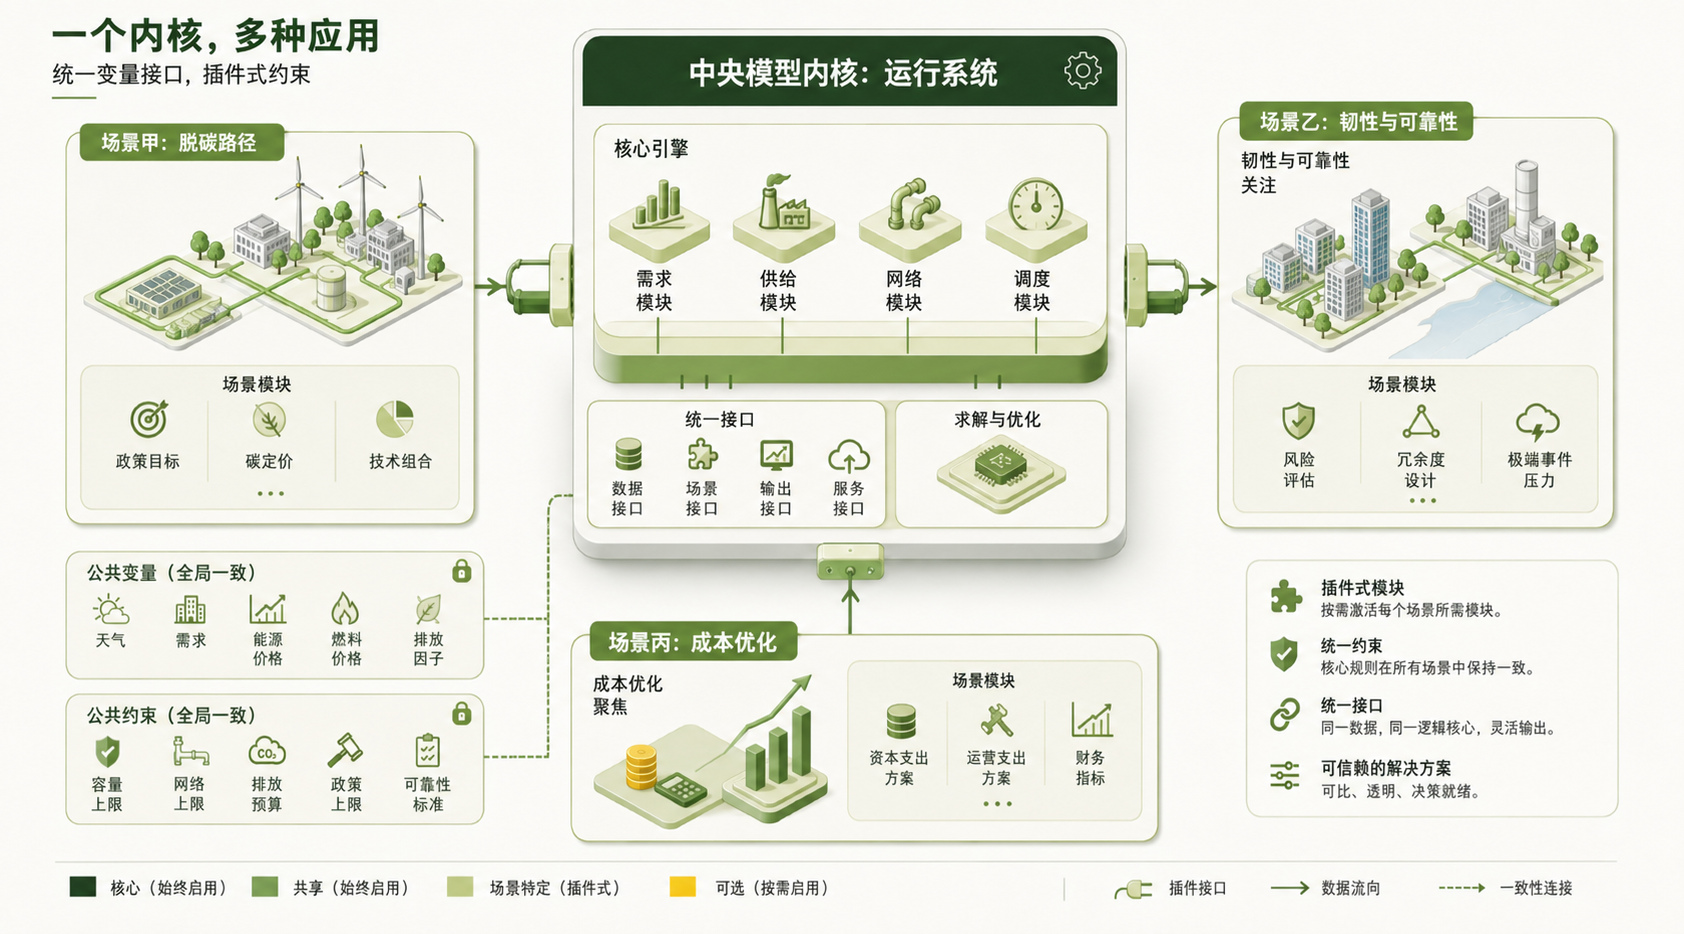
\includegraphics[width=0.714\textwidth,height=0.34\textheight,keepaspectratio]{media/model-figures/130.jpg}
\caption{创新点六：同一内核跨三场景迁移}
\label{fig:model-130}
\end{figure}

\subsection{模型局限}

原始聚合算例采用固定温位的MILP、有限情景重算和关键断面校核，连续温差---流量、指数温降和非凸水力不直接纳入主模型。建筑热状态采用聚合节点的单一等效热容，未计算房间级温度；热湿、噪声、地源多年动态等模块未在本次算例中启用。模型结果用于规划比较，不能替代施工图、设备选型、地质勘察、环保审批和配电潮流校核。

\enlargethispage{2\baselineskip}
\subsection{结论}

本文将三类供热转型问题表述为资产配置、空间组织、带温位能流、建筑热状态与储热协同优化，并保留分阶段规划接口。三个场景共享公用内核，并分别加载既有热网改造、分散设施选址和夏热冬冷地区供热形态约束。

乌鲁木齐场景获得投资---运行联合解；固原与武汉采用锚定两阶段方法，形成固定投资模式下的全供暖季运行结果。三个场景均完成守恒、容量、储热和可靠性检查；连续水力、房间级温度、热湿与噪声等内容作为后续工程扩展，不列入本次结果结论。

\clearpage
\begin{center}{\heiti\sihao 参考文献}\end{center}
\phantomsection
\addcontentsline{toc}{section}{参考文献}
\begin{refsectionflush}
\refentry{1}{中国建筑科学研究院有限公司.
面向供热格局变革的城镇供热源荷匹配与规划寻优模型构建比赛方案{[}R{]}.
2026.}
\refentry{2}{江亿, 付林, 夏建军, 谢晓云, 吴彦廷, 胡姗.
构建新型零碳热力系统{[}J{]}. 中国工程科学, 2025, 27(5): 1--18. DOI:
10.15302/J-SSCAE-2025.08.025.}
\refentry{3}{Lin Q, Lu S, Yue L, Li B, Zhu H. Research on low-carbon district
heating system planning approach based on thermal energy grade and
integrated demand response{[}EB/OL{]}. SSRN preprint 5082363,
2024/2025（未同行评审预印本）.}
\refentry{4}{Ceruti A, Lambert J, Spliethoff H. Integrating renewable energy
and thermal storage in district heating networks: A design optimization
approach{[}J{]}. Energy Conversion and Management, 2025, 345: 120323.
DOI: 10.1016/j.enconman.2025.120323.}
\refentry{5}{Chen J, Lv H, Ding L, et al.~Multi-objective optimization for
the operation of district heating systems considering flexibility and
economy{[}J{]}. Applied Thermal Engineering, 2025, 263: 125395. DOI:
10.1016/j.applthermaleng.2024.125395.}
\refentry{6}{Lyu Z, Huang M, Liu B, Liu Y. Robust optimization of regional
integrated energy systems considering thermal comfort and uncertainty in
heat networks{[}J{]}. Applied Thermal Engineering, 2025, 275: 126895.
DOI: 10.1016/j.applthermaleng.2025.126895.}
\refentry{7}{崔梦颖, 殷勇高, 赵栋霖, 黄钰希, 曹博文.
地埋管跨季节储热耦合热泵供暖系统性能与经济性分析{[}J{]}. 储能科学与技术,
2026, 15(3): 983--992. DOI: 10.19799/j.cnki.2095-4239.2026.0107.}
\refentry{8}{崔杨, 姜涛, 仲悟之, 崔成伟, 赵钰婷.
考虑风电消纳的区域综合能源系统源荷协调经济调度{[}J{]}. 电网技术, 2020,
44(7): 2474--2482. DOI: 10.13335/j.1000-3673.pst.2019.2317.}
\refentry{9}{李仲博.
基于数字孪生的城镇供热系统按需精准调控技术研究与应用{[}D{]}. 杭州:
浙江大学, 2023.}
\refentry{10}{Paule D, Pakere I, Pubule J, Blumberga D. Optimising
multi-energy community hubs for decarbonisation and energy system
flexibility{[}J{]}. Smart Energy, 2025, 20: 100214. DOI:
10.1016/j.segy.2025.100214.}
\refentry{11}{Zhang Y, Campana P E, Yang Y, et al.~Energy flexibility from
the consumer: Integrating local electricity and heat supplies in a
building{[}EB/OL{]}.}
\refentry{12}{Lu H, Khanna N, Feng W, et al.~China's Electrification
Pathways: Findings from the China Energy Outlook 2022{[}R{]}. Lawrence
Berkeley National Laboratory, 2022.}
\refentry{13}{赵丽丽. 东北农村冬季清洁供暖技术节能改造应用技术研究{[}J{]}.
节能, 2025, 44(11): 88--91. DOI: 10.3969/j.issn.1004-7948.2025.11.018.}
\refentry{14}{白孝轩, 谈润芃, 李朋, 等.
民用燃煤碳排放特征及电能替代减排路径优化{[}J/OL{]}. 环境科学研究, 2026.
DOI: 10.13198/j.issn.1001-6929.2026.06.17.}
\refentry{15}{Wang S, Su H, Chen C, et al.~Natural gas shortages during the
``coal-to-gas'' transition in China have caused a large redistribution
of air pollution{[}EB/OL{]}. arXiv:2004.09585, 2020.}
\refentry{16}{Wang X, Xia L, Bales C, et al.~A systematic review of recent
air source heat pump systems assisted by solar thermal, photovoltaic and
photovoltaic/thermal sources{[}EB/OL{]}. arXiv:2102.09797, 2021.}
\refentry{17}{Xiong C, Hassan M S. Renewable heat policy in China:
Development, achievement, and effectiveness{[}J{]}. Sustainability,
2022, 14: 9297. DOI: 10.3390/su14159297.}
\refentry{18}{Fiorentini M, Baldini L. Control-oriented modelling and
operational optimization of a borehole thermal energy storage{[}J{]}.
Applied Thermal Engineering, 2021: 117518. DOI:
10.1016/j.applthermaleng.2021.117518.}
\refentry{19}{Takam P H, Wunderlich R. Model order reduction for the
input--output behavior of a geothermal energy storage{[}J{]}. Journal of
Engineering Mathematics, 2024, 148: 12. DOI: 10.1007/s10665-024-10398-4.}
\refentry{20}{Li H, Svendsen S. Energy and exergy analysis of low temperature
district heating network{[}J{]}. Energy, 2012, 45(1): 237--246. DOI:
10.1016/j.energy.2012.03.056.}
\refentry{21}{Lund H, Werner S, Wiltshire R, et al.~4th Generation District
Heating (4GDH): Integrating smart thermal grids into future sustainable
energy systems{[}J{]}. Energy, 2014, 68: 1--11. DOI:
10.1016/j.energy.2014.02.089.}
\refentry{22}{Capone M, Guelpa E, Verda V. Potential for supply temperature
reduction of existing district heating substations{[}J{]}. Energy, 2023,
285: 128597. DOI: 10.1016/j.energy.2023.128597.}
\refentry{23}{IPCC. 2006 IPCC Guidelines for National Greenhouse Gas
Inventories, Volume 2: Energy{[}R{]}. Hayama: IGES, 2006.}
\refentry{24}{国务院办公厅. 国务院办公厅关于转发国家发展改革委、住房城乡建设部《加快推动建筑领域节能降碳工作方案》的通知{[}EB/OL{]}. \url{https://www.mee.gov.cn/zcwj/gwywj/202403/t20240318\_1068599.shtml}, 访问时间（2026年7月17日）.}
\refentry{25}{国家发展和改革委员会. 加强建筑全过程节能降碳管理，推动建筑领域绿色低碳发展{[}EB/OL{]}. \url{https://www.ndrc.gov.cn/xxgk/jd/jd/202403/t20240321\_1365112.html}, 访问时间（2026年7月17日）.}
\refentry{26}{International Energy Agency. Renewable heat: Renewables 2025{[}EB/OL{]}. \url{https://www.iea.org/reports/renewables-2025/renewable-heat}, 访问时间（2026年7月17日）.}
\refentry{27}{European Commission. Heating and cooling{[}EB/OL{]}. \url{https://energy.ec.europa.eu/topics/energy-efficiency/heating-and-cooling\_en}, 访问时间（2026年7月17日）.}

\refentry{28}{Bacher P, Madsen H. Identifying suitable models for the heat dynamics of buildings{[}J{]}. Energy and Buildings, 2011, 43(7): 1511--1522. DOI: \url{https://doi.org/10.1016/j.enbuild.2011.02.005}.}
\refentry{29}{Miller C, Kathirgamanathan A, Picchetti B, et al. The Building Data Genome Project 2, energy meter data from the ASHRAE Great Energy Predictor III competition{[}J{]}. Scientific Data, 2020, 7: 368. DOI: \url{https://doi.org/10.1038/s41597-020-00712-x}.}
\refentry{30}{TICA. V-FORCE Full DC Inverter Modular Chiller (Heat Pump){[}Z{]}. 产品样本，PDF第14--15页. 经销商存档：\url{https://dec.com.pk/assets/images/products/tica/3-Inverter-modular-chiller.pdf}. 采用已冻结副本.}
\refentry{31}{NASA POWER. Hourly API{[}EB/OL{]}. \url{https://power.larc.nasa.gov/docs/services/api/temporal/hourly/}. 三城逐时数据查询与原响应随证据保存.}
\refentry{32}{Mavrotas G. Effective implementation of the $\varepsilon$-constraint method in Multi-Objective Mathematical Programming problems{[}J{]}. Applied Mathematics and Computation, 2009, 213(2): 455--465. DOI: 10.1016/j.amc.2009.03.037.}
\refentry{33}{Liao X, Wang W, Zhou Y. Investigating the Energy-Saving Effectiveness of Envelope Retrofits and Photovoltaic Systems: A Case Study of a Hotel in Urumqi{[}J{]}. Sustainability, 2023, 15(13): 9926. DOI: \url{https://doi.org/10.3390/su15139926}. 现场照片按CC BY 4.0许可引用.}
\end{refsectionflush}



% 仅修正附录目录跳转锚点，模型附录源文件保持不变。
\begingroup
\let\paperAppendixContents\addcontentsline
\renewcommand{\addcontentsline}[3]{\phantomsection\paperAppendixContents{#1}{#2}{#3}}
% !TeX root = ../main.tex
% !TeX program = xelatex
% !TeX encoding = UTF-8
\clearpage
\section*{附录1\quad 场景约束与校核式}
\addcontentsline{toc}{section}{\texorpdfstring{附录1\quad 场景约束与校核式}{附录1 场景约束与校核式}}

本附录保留原三城规划框架，按“约束对象—物理作用—启用条件”阅读。规划容量在对应运行窗口内保持不变，逐时出力和状态共同满足正文的能量平衡。场景专用式中包含扩展接口，实际采用范围以配置矩阵、附录4的数据登记和附录5的运行记录为准。

\begin{table}[H]
\centering\small
\caption{规划变量、运行量与状态的衔接}
\begin{tabularx}{\linewidth}{@{}L{0.16\linewidth}L{0.32\linewidth}Y@{}}
\toprule
类别 & 原模型中的对象 & 与其余环节的连接\\\midrule
规划变量 & 热源新增与退役、管段与储热容量、配电增容 & 限定每小时可用出力、输送及调节能力；固定投资复算中不再增加容量\\
运行变量 & 热源出力、管段热流、储热充放、购电 & 在同一小时满足节点温位、电力和资源约束\\
状态变量 & 聚合热状态、储热量；逐楼分支的室温 & 由前一时段递推；初末边界和逐时上下界限制跨时段调节\\
复核量 & 守恒残差、容量利用率及已启用工程检查 & 与可行解和求解间隙分别记录，限定结果可采用的范围\\
\bottomrule
\end{tabularx}
\end{table}

各式后的专用约束用于说明场景差异；它们不意味着三城主算例同时启用了全部选址、热湿、地源或连续水力模块。原聚合模型与独立逐楼热状态验证分别留存配置。

\subsection*{A\quad 乌鲁木齐场景}
\addcontentsline{toc}{subsection}{A 乌鲁木齐场景}

\subsubsection*{A.1\quad 热源退役与替代}

燃煤热源退役量不得超过上一阶段已投运容量；达到政策退役年限后，对应容量固定为零：
\begin{equation}
K_{\mathrm{coal},y}^{\mathrm{ret}}\leq K_{\mathrm{coal},y-1}^{\mathrm{exist}},
\qquad y\geq y^{\mathrm{deadline}}\Rightarrow K_{\mathrm{coal},y}^{\mathrm{exist}}=0.
\end{equation}
退役容量由清洁热源、储热有效容量和备用容量共同替代：
\begin{equation}
K_{\mathrm{coal},y}^{\mathrm{ret}}\leq
K_y^{\mathrm{clean,new}}+K_y^{\mathrm{storage,credit}}+K_y^{\mathrm{reserve}}.
\end{equation}
其中，$K_y^{\mathrm{storage,credit}}$表示设计峰值时段可持续提供的放热功率，不等同于储热装置的额定储能量。

\subsubsection*{A.2\quad 余热与热泵}

工业余热利用量受资源供给与回收效率限制：
\begin{equation}
0\leq Q_t^{\mathrm{waste}}\leq\eta^{\mathrm{recovery}}Q_t^{\mathrm{available}}.
\end{equation}
热泵的热量转换、出力和配电边界为
\begin{align}
Q_t^{\mathrm{HP}}&=COP_tP_t^{\mathrm{HP}},\\
0\leq Q_t^{\mathrm{HP}}&\leq\overline Q^{\mathrm{HP}}u_t^{\mathrm{HP}},\\
P_t^{\mathrm{HP}}+P_t^{\mathrm{base}}+P_t^{\mathrm{pump}}&\leq\overline P^{\mathrm{grid}}.
\end{align}
$COP_t$随热源侧温度、用户侧供水温度和部分负荷率变化。

\subsubsection*{A.3\quad 温位与水力}

热源$k$与温位$g$的兼容参数定义为
\begin{equation}
A_{kg}^{\mathrm{grade}}=
\begin{cases}
1,&T_k^{\mathrm{src,min}}\geq T_g^{\mathrm{sup}}+\Delta T^{\mathrm{hx}},\\
0,&\text{其他情况}.
\end{cases}
\end{equation}
直接供热量满足$0\leq Q_{k,g,t}^{\mathrm{direct}}\leq A_{kg}^{\mathrm{grade}}\overline Q_k$。关键管段的最大流量利用率为
\begin{equation}
\lambda_e^{\mathrm{flow}}=
\frac{\max_t|\dot m_{e,t}^{\mathrm{exist}}+\dot m_{e,t}^{\mathrm{new}}|}{\overline{\dot m}_e}\leq1.
\end{equation}
管段出口温度采用连续温降模型校核：
\begin{equation}
T_{e,t}^{\mathrm{out}}=T_{e,t}^{\mathrm{env}}+
(T_{e,t}^{\mathrm{in}}-T_{e,t}^{\mathrm{env}})
\exp\left(-\frac{U_eL_e}{\dot m_{e,t}c_p}\right).
\end{equation}
最远换热站的温度裕度满足
\begin{equation}
\Delta T_{n^{\mathrm{far}}}^{\mathrm{margin}}=
\min_t\left(T_{n^{\mathrm{far}},t}^{\mathrm{sup}}-T_{n^{\mathrm{far}},t}^{\mathrm{req}}-\Delta T^{\mathrm{hx}}\right)\geq0.
\end{equation}

\subsubsection*{A.4\quad 回水与可靠性}

换热站供热量、回水温度和最低温差满足
\begin{equation}
Q_{n,t}=\dot m_{n,t}c_p(T_{n,t}^{\mathrm{sup}}-T_{n,t}^{\mathrm{ret}}),
\quad T_{n,t}^{\mathrm{ret}}\leq\overline T_n^{\mathrm{ret}},
\quad T_{n,t}^{\mathrm{sup}}-T_{n,t}^{\mathrm{ret}}\geq\underline{\Delta T}_n.
\end{equation}
关键热源$k$退出时，剩余热源与储热逐时承担负荷：
\begin{equation}
\sum_{j\neq k}Q_{j,t}^{\mathrm{avail}}+Q_t^{\mathrm{storage,dis}}\geq D_t.
\end{equation}
寒潮场景同步修正室外温度、负荷和余热可用量，并要求各时段失供量为零：
\begin{align}
T_t^{\mathrm{out,cold}}&=T_t^{\mathrm{out}}-\Delta T^{\mathrm{cold}},
&D_t^{\mathrm{cold}}&=\alpha_DD_t,\\
Q_t^{\mathrm{waste,cold}}&=\alpha_WQ_t^{\mathrm{waste}},
&Q_t^{\mathrm{un,cold}}&=0.
\end{align}

\subsubsection*{A.5\quad 末端改造}

建筑末端改造变量$z_b^{\mathrm{retro}}\in\{0,1\}$决定最低供水温度：
\begin{equation}
T_b^{\mathrm{req}}=(1-z_b^{\mathrm{retro}})T_b^{\mathrm{old}}+z_b^{\mathrm{retro}}T_b^{\mathrm{new}}.
\end{equation}
管网降温方案同时满足$T_{b,t}^{\mathrm{sup}}\geq T_b^{\mathrm{req}}+\Delta T_b^{\mathrm{hx}}$、改造预算约束和室内最低温度约束。

\subsection*{B\quad 固原场景}
\addcontentsline{toc}{subsection}{B 固原场景}

\subsubsection*{B.1\quad 选址与连通}

候选热源建设、用户分配、服务半径和容量满足
\begin{align}
z_i^{\mathrm{site}}&\in\{0,1\},\qquad
\sum_i x_{i,b}=1,\qquad x_{i,b}\leq z_i^{\mathrm{site}},\\
d_{i,b}x_{i,b}&\leq\overline d_i,\qquad
\sum_bD_b^{\mathrm{peak}}x_{i,b}\leq K_i.
\end{align}
候选管段状态限制热流，热源与用户之间必须存在有效路径：
\begin{equation}
|F_{e,t}|\leq\overline F_ez_e^{\mathrm{pipe}},
\qquad x_{i,b}\leq z_e^{\mathrm{pipe}},
\quad \forall e\in\mathcal P_{i,b}.
\end{equation}
逐段约束保证被分配用户对应路径上的每一条候选管段均已建设；节点热平衡进一步保证路径上的能流连续。

\subsubsection*{B.2\quad 燃料库存}

生物质供热、到货与库存按同一时间轴计算：
\begin{align}
Q_{i,t}^{\mathrm{bio}}\Delta t&=\eta_i^{\mathrm{bio}}H_i^{\mathrm{LHV}}B_{i,t}^{\mathrm{use}},\\
I_{i,t}&=I_{i,t-1}+B_{i,t}^{\mathrm{arrive}}-B_{i,t}^{\mathrm{use}},\\
0\leq I_{i,t}&\leq\overline I_i,\qquad
0\leq B_{i,t}^{\mathrm{arrive}}\leq\overline B_i^{\mathrm{arrive}}.
\end{align}
库存不足时，锅炉出力同步受限：
\begin{equation}
Q_{i,t}^{\mathrm{bio}}\Delta t\leq\eta_i^{\mathrm{bio}}H_i^{\mathrm{LHV}}
(I_{i,t-1}+B_{i,t}^{\mathrm{arrive}}).
\end{equation}
其中$Q^{\mathrm{bio}}$以kW计，$H^{\mathrm{LHV}}$以kWh/kg计，$B^{\mathrm{use}}$以kg计，$\Delta t$以h计。

\subsubsection*{B.3\quad 微网与孤岛}

微网电力平衡及配电容量约束为
\begin{multline}
P_{i,t}^{\mathrm{imp}}+P_{i,t}^{\mathrm{PV}}+P_{i,t}^{\mathrm{bat,dis}}
=P_{i,t}^{\mathrm{base}}+P_{i,t}^{\mathrm{HP}}+P_{i,t}^{\mathrm{EB}}
+P_{i,t}^{\mathrm{pump}}+P_{i,t}^{\mathrm{bat,ch}},\\
P_{i,t}^{\mathrm{imp}}\leq\overline P_i^{\mathrm{grid}}.
\end{multline}
外部电网或单一热源故障时，可用热源与储热满足关键用户负荷：
\begin{equation}
\sum_{k\in\mathcal K_i^{\mathrm{available}}}Q_{k,t}
+Q_{i,t}^{\mathrm{storage,dis}}\geq D_{i,t}^{\mathrm{critical}}.
\end{equation}
完全孤岛状态下，本地电源还应覆盖热泵、电锅炉和循环泵的基本用电。

\subsubsection*{B.4\quad 防冻结与可负担性}

低温运行满足
\begin{equation}
\dot m_{e,t}\geq\dot m_e^{\min},\qquad
T_{e,t}^{\mathrm{ret}}\geq T_e^{\mathrm{freeze}}.
\end{equation}
同时约束运维距离$d_i^{\mathrm{maint}}\leq\overline d_i^{\mathrm{maint}}$和居民供热费用$C_b^{\mathrm{heat}}\leq\overline C_b^{\mathrm{afford}}$。

\subsection*{C\quad 武汉场景}
\addcontentsline{toc}{subsection}{C 武汉场景}

\subsubsection*{C.1\quad 系统形态与多类负荷}

每个区域选择一种基本供热形态：
\begin{equation}
z_i^{\mathrm{building}}+z_i^{\mathrm{station}}+z_i^{\mathrm{LTN}}+z_i^{\mathrm{5GDHC}}=1.
\end{equation}
供热与生活热水平衡、供冷转换和总用电分别为
\begin{align}
Q_{i,t}^{\mathrm{source}}+Q_{i,t}^{\mathrm{storage,dis}}
&=D_{i,t}^{\mathrm{heat}}+D_{i,t}^{\mathrm{DHW}}+Q_{i,t}^{\mathrm{storage,ch}},\\
Q_{i,t}^{\mathrm{cool}}&=COP_{i,t}^{\mathrm{cool}}P_{i,t}^{\mathrm{cool}},\\
P_{i,t}^{\mathrm{total}}&=P_{i,t}^{\mathrm{base}}+P_{i,t}^{\mathrm{heat}}
+P_{i,t}^{\mathrm{cool}}+P_{i,t}^{\mathrm{DHW}}+P_{i,t}^{\mathrm{pump}}.
\end{align}

\subsubsection*{C.2\quad 间歇运行与舒适度}

启动变量和最小连续运行时间满足
\begin{equation}
u_{b,t}-u_{b,t-1}\leq v_{b,t}^{\mathrm{start}},\qquad
\sum_{\tau=t}^{t+T_b^{\min}-1}u_{b,\tau}\geq T_b^{\min}v_{b,t}^{\mathrm{start}}.
\end{equation}
供暖期和供冷期分别设置室温范围，相对湿度和最低新风量满足
\begin{equation}
RH_b^{\min}\leq RH_{b,t}\leq RH_b^{\max},\qquad
V_{b,t}^{\mathrm{vent}}\geq\underline V_b^{\mathrm{vent}}.
\end{equation}

\subsubsection*{C.3\quad 结露与除霜}

室内表面和低温管网均应高于露点并保留安全裕度：
\begin{equation}
T_{b,t}^{\mathrm{surface}}\geq T_{b,t}^{\mathrm{dew}}+\Delta T^{\mathrm{safe}},
\qquad T_{e,t}^{\mathrm{sup}}\geq T_{e,t}^{\mathrm{dew}}+\Delta T_e^{\mathrm{safe}}.
\end{equation}
空气源热泵除霜期间的实际供热量和耗电量为
\begin{equation}
Q_t^{\mathrm{HP,actual}}=(1-\phi_t^{\mathrm{defrost}})Q_t^{\mathrm{HP,rated}},
\qquad P_t^{\mathrm{HP,actual}}=P_t^{\mathrm{HP,rated}}+P_t^{\mathrm{defrost}}.
\end{equation}

\subsubsection*{C.4\quad 地源、噪声与配电}

地源系统年度取热与排热比值约束为
\begin{equation}
r^{\min}\sum_tQ_t^{\mathrm{inj}}\Delta t
\leq\sum_tQ_t^{\mathrm{ext}}\Delta t
\leq r^{\max}\sum_tQ_t^{\mathrm{inj}}\Delta t.
\end{equation}
其中$Q^{\mathrm{ext}}$为从地下取热功率，$Q^{\mathrm{inj}}$为向地下排热功率，$\Delta t$为时间步长。该式属于可选约束，本次三个算例均未启用。
正常时段和夜间分别设置噪声上限。楼栋配电容量满足
\begin{equation}
P_{b,t}^{\mathrm{HP}}+P_{b,t}^{\mathrm{cool}}+P_{b,t}^{\mathrm{DHW}}+P_{b,t}^{\mathrm{base}}
\leq P_b^{\mathrm{exist}}+K_b^{\mathrm{grid,new}}.
\end{equation}

\subsection*{D\quad 统一校核}
\addcontentsline{toc}{subsection}{D 统一校核}

以下汇总框架的基础检查目标，按对应记录启用的模型分支分别执行：
\begin{align}
\max_t|r_t^{\mathrm{heat}}|&\leq\varepsilon_Q,&
\max_t|r_t^{\mathrm{storage}}|&\leq\varepsilon_E,\\
\theta_b^{\min}\leq\theta_{b,t}^{a}&\leq\theta_b^{\max},&
\lambda_e^{\mathrm{flow}}&\leq1,\\
P_{n,t}^{\mathrm{imp}}&\leq\overline P_n^{\mathrm{grid}},&
U^{\mathrm{un}}&=0.
\end{align}
乌鲁木齐增加资产退役、温位匹配、管网降温与寒潮保供校核；固原增加热源选址、微网连通、燃料库存、孤岛运行和防冻结校核；武汉增加冷热水耦合、热湿舒适、结露、除霜、地源平衡、噪声和楼栋配电校核。

\endgroup

\section*{附录2\quad 符号与缩略语说明}
\phantomsection
\addcontentsline{toc}{section}{\texorpdfstring{附录2\quad 符号与缩略语说明}{附录2 符号与缩略语说明}}

本文仅列出模型中频繁使用的典型符号。程序输入与逐时调度采用kW、kWh和kg，汇总表可换算为MW、MWh和t；换算关系分别为$1~\mathrm{MW}=10^3~\mathrm{kW}$、$1~\mathrm{MWh}=10^3~\mathrm{kWh}$和$1~\mathrm{t}=10^3~\mathrm{kg}$。摄氏温差与开尔文温差数值相同；涉及火用计算时，绝对温度由$T(\mathrm K)=\theta({}^{\circ}\mathrm C)+273.15$换算。

\begin{table}[H]
\centering
\caption{典型符号说明}
\begin{tabular}{p{0.16\textwidth}p{0.43\textwidth}p{0.28\textwidth}}
\toprule
符号 & 含义 & 单位\\
\midrule
$c$ & 供热转型场景编号（C1、C2、C3） & --\\
$y$ & 规划阶段或年份 & --\\
$t$ & 运行时段 & h\\
$\omega$ & 不确定情景 & --\\
$n$ & 网络节点或建筑节点 & --\\
$k$ & 设备类型 & --\\
$x$ & 第一阶段规划决策变量 & --\\
$q_\omega$ & 情景$\omega$下运行变量 & --\\
$K$ & 设备容量变量 & kW（汇总时可换算为MW）\\
$SOC$ & 储能状态变量 & kWh（汇总时可换算为MWh）\\
$C$ & 聚合节点等效热容 & kWh/K\\
$R$ & 等效热阻 & K/kW\\
$C_{net}$ & 生命周期净成本 & 元\\
$EENS$ & 期望失供能量 & MWh\\
$COP$ & 热泵性能系数 & --\\
\bottomrule
\end{tabular}
\end{table}

常用缩略语包括：MILP（混合整数线性规划）、CHP（热电联产）、TES（储热系统）、BTES（跨季节地埋管储热）、CVaR（条件风险价值）、EENS（期望失供能量）。

% !TeX root = ../main.tex
\clearpage
\section*{附录3\quad 核心代码（Python详编）}
\phantomsection\label{appendix:code}
\addcontentsline{toc}{section}{附录3：核心代码（Python详编）}

本附录沿用原有12段代码的顺序，补入共享热资源、逐楼热状态、配电边界、硬约束权重及紧凑启停实现，共17段、1066行原代码和224行补充注释。代码均从随包R8O固定源码连续节选，按输入输出、实现思路、关键注释和结果核对展开；正文模型与算法结构保持原样。

\textbf{阅读顺序。}第1段说明入口；第2--4段连接建筑、储热与节点热平衡；第5--6段完成稀疏求解及数值复核；第7--8段将规划资产交给连续供暖季运行；第9--12段说明多目标、权重诊断和管网反馈。新增第13--15段补齐跨模块的物理衔接，第16--17段展示权重优化与整数规模压缩的具体实现。

显示行号从每段1开始并包含新增注释，索引给出原文件准确行号。\path{code_annotated_r8p_a4}内保存原样节选、注释版及逐行映射，\path{code_annotation_manifest_a4.json}记录来源和指纹。删除新增注释后，原代码行及可执行token一致；可以独立解析的片段另核对AST。代码排版沿用原有配色、字体与框线，上下文片段仍须在完整工程中调用。

源码说明各接口的实现，实验是否执行及其结果以对应运行记录为准。代表日规划、固定投资复算、两阶段端点和独立碳帽扫描分别保留执行身份；下文在相关代码处说明开关和衔接条件。

\begin{longtable}{@{}cL{0.34\linewidth}L{0.54\linewidth}@{}}
\caption{详编代码来源与正文方法对应}\label{tab:code-index-a4}\\
\toprule
序号 & 文件与原行号 & 对应内容\\\midrule
\endfirsthead
\toprule 序号 & 文件与原行号 & 对应内容\\\midrule
\endhead
\bottomrule\endfoot
1 & \path{unified_cli.py}，93--118 & 单次求解入口与导出\\
2 & \path{building_thermal.py}，31--46 & 逐楼1R1C精确离散系数\\
3 & \path{model.py}，1391--1471 & 储热容量、运行与状态边界\\
4 & \path{model.py}，1603--1697 & 节点温位逐时热平衡\\
5 & \path{linear.py}，177--205 & SciPy稀疏MILP求解接口\\
6 & \path{linear.py}，40--105 & 独立数值与守恒残差复核\\
7 & \path{experiments.py}，13--147 & 完整投资冻结与费用账本\\
8 & \path{heating_season.py}，183--246 & 固定投资的连续供暖季复算\\
9 & \path{model.py}，2829--2888 & 带主目标容差的两阶段端点\\
10 & \path{experiments.py}，351--411 & 独立碳帽采样与非支配筛选\\
11 & \path{representative_adoption.py}，48--94 & 代表日硬能量约束可行性诊断\\
12 & \path{network_feedback.py}，440--481 & 有限模式管网反馈与失败处理\\
13 & \path{physical_extensions.py}，25--79 & 热源出力的上游余热共用约束\\
14 & \path{building_thermal.py}，463--525 & 逐楼RC状态、舒适边界与节点交付量\\
15 & \path{model.py}，2030--2089 & 逐时配电接入容量及可靠容量方法入口\\
16 & \path{hard_weight_calibration.py}，13--97 & 硬能量守恒下的最小一维W1权重线性规划\\
17 & \path{model.py}，938--1018 & 热源启停三行紧凑凸包与容量关联爬坡\\
\end{longtable}

正文算法\ref{alg:season-workflow}对应规划与固定投资复算；算法\ref{alg:epsilon-workflow}对应独立碳帽接口。第16段补充的是代表日权重优化本体，第11段则是等式与下界能否同时成立的诊断，两者作用分开。

\Needspace{12\baselineskip}
\subsection*{1．单次求解入口与导出}
主入口中没有政策路径时的单次求解分支；配置可以按需展开相关天气场景，随后统一求解和导出。

\noindent\textbf{输入：}当前profile的配置路径、逐时输入路径、可选场景说明及求解预算。\par
\noindent\textbf{输出：}投资、逐时运行、汇总指标与场景结果文件。该节选依赖外层profile循环。\par

\noindent\textbf{实现思路。}该入口负责把配置、逐时输入和求解预算连接起来。需求列从节点配置取得，避免在场景展开时漏掉某一节点；随后将场景风险设置写入配置副本，再统一校验。\path{HeatPlanningModel}接收校验后的同一组输入，导出也使用模型实际采用的时序，因而输入、求解与结果文件可以一一对应。

{\small 来源：\path{unified_cli.py}，原第93--118行；26行原代码、10行补充注释。}\par

\begingroup
\setstretch{1.0}
\begin{Verbatim}[commandchars=\\\{\},numbers=left,firstnumber=1,stepnumber=1,fontsize=\fontsize{9.5}{11.5}\selectfont,breaklines=true,breakanywhere=true,frame=single,framesep=3mm,numbersep=5pt,rulecolor=\color{black},xleftmargin=18pt]
\PYG{k}{else}\PYG{p}{:}
    \PYG{c+c1}{\PYGZsh{} \CJKCode{配置与时序共同定义算例身份；本段不自动启动碳帽扫描。}}
    \PYG{n}{config}\PYG{p}{,} \PYG{n}{frame} \PYG{o}{=} \PYG{n}{load\PYGZus{}inputs}\PYG{p}{(}\PYG{n}{config\PYGZus{}path}\PYG{p}{,} \PYG{n}{timeseries\PYGZus{}path}\PYG{p}{)}
    \PYG{c+c1}{\PYGZsh{} \CJKCode{仅在提供场景文件时展开不确定场景；无文件则沿用读入时序。}}
    \PYG{k}{if} \PYG{n}{scenario\PYGZus{}specs\PYGZus{}path}\PYG{p}{:}
        \PYG{n}{specs} \PYG{o}{=} \PYG{n}{yaml}\PYG{o}{.}\PYG{n}{safe\PYGZus{}load}\PYG{p}{(}\PYG{n}{scenario\PYGZus{}specs\PYGZus{}path}\PYG{o}{.}\PYG{n}{read\PYGZus{}text}\PYG{p}{(}\PYG{n}{encoding}\PYG{o}{=}\PYG{l+s+s2}{\PYGZdq{}}\PYG{l+s+s2}{utf\PYGZhy{}8}\PYG{l+s+s2}{\PYGZdq{}}\PYG{p}{)}\PYG{p}{)}
        \PYG{c+c1}{\PYGZsh{} \CJKCode{按节点配置收集需求列，保持场景扩展与需求接口一致。}}
        \PYG{n}{demand\PYGZus{}columns} \PYG{o}{=} \PYG{p}{[}
            \PYG{n}{column} \PYG{k}{for} \PYG{n}{node} \PYG{o+ow}{in} \PYG{n}{config}\PYG{p}{[}\PYG{l+s+s2}{\PYGZdq{}}\PYG{l+s+s2}{nodes}\PYG{l+s+s2}{\PYGZdq{}}\PYG{p}{]}
            \PYG{k}{for} \PYG{n}{column} \PYG{o+ow}{in} \PYG{n}{node}\PYG{o}{.}\PYG{n}{get}\PYG{p}{(}\PYG{l+s+s2}{\PYGZdq{}}\PYG{l+s+s2}{demand\PYGZus{}columns}\PYG{l+s+s2}{\PYGZdq{}}\PYG{p}{,} \PYG{p}{\PYGZob{}}\PYG{p}{\PYGZcb{}}\PYG{p}{)}\PYG{o}{.}\PYG{n}{values}\PYG{p}{(}\PYG{p}{)}
        \PYG{p}{]}
        \PYG{n}{frame} \PYG{o}{=} \PYG{n}{build\PYGZus{}correlated\PYGZus{}northern\PYGZus{}scenario\PYGZus{}bundle}\PYG{p}{(}
            \PYG{n}{frame}\PYG{p}{,} \PYG{n}{demand\PYGZus{}columns}\PYG{p}{,} \PYG{n}{specs}\PYG{p}{[}\PYG{l+s+s2}{\PYGZdq{}}\PYG{l+s+s2}{scenarios}\PYG{l+s+s2}{\PYGZdq{}}\PYG{p}{]}\PYG{p}{,}
            \PYG{c+c1}{\PYGZsh{} period\PYGZus{}weight\CJKCode{是代表时段权重，不等同于额外的物理小时步长。}}
            \PYG{n}{period\PYGZus{}weight}\PYG{o}{=}\PYG{n+nb}{float}\PYG{p}{(}\PYG{n}{specs}\PYG{o}{.}\PYG{n}{get}\PYG{p}{(}\PYG{l+s+s2}{\PYGZdq{}}\PYG{l+s+s2}{period\PYGZus{}weight}\PYG{l+s+s2}{\PYGZdq{}}\PYG{p}{,} \PYG{n}{config}\PYG{p}{[}\PYG{l+s+s2}{\PYGZdq{}}\PYG{l+s+s2}{planning}\PYG{l+s+s2}{\PYGZdq{}}\PYG{p}{]}\PYG{o}{.}\PYG{n}{get}\PYG{p}{(}\PYG{l+s+s2}{\PYGZdq{}}\PYG{l+s+s2}{representative\PYGZus{}day\PYGZus{}weight}\PYG{l+s+s2}{\PYGZdq{}}\PYG{p}{,} \PYG{l+m+mf}{1.0}\PYG{p}{)}\PYG{p}{)}\PYG{p}{)}\PYG{p}{,}
        \PYG{p}{)}
        \PYG{c+c1}{\PYGZsh{} \CJKCode{复制后修改风险设置，保留此前读入的配置对象。}}
        \PYG{n}{config} \PYG{o}{=} \PYG{n}{copy}\PYG{o}{.}\PYG{n}{deepcopy}\PYG{p}{(}\PYG{n}{config}\PYG{p}{)}
        \PYG{n}{config}\PYG{p}{[}\PYG{l+s+s2}{\PYGZdq{}}\PYG{l+s+s2}{planning}\PYG{l+s+s2}{\PYGZdq{}}\PYG{p}{]}\PYG{p}{[}\PYG{l+s+s2}{\PYGZdq{}}\PYG{l+s+s2}{risk}\PYG{l+s+s2}{\PYGZdq{}}\PYG{p}{]} \PYG{o}{=} \PYG{n+nb}{dict}\PYG{p}{(}\PYG{n}{specs}\PYG{o}{.}\PYG{n}{get}\PYG{p}{(}\PYG{l+s+s2}{\PYGZdq{}}\PYG{l+s+s2}{risk}\PYG{l+s+s2}{\PYGZdq{}}\PYG{p}{,} \PYG{p}{\PYGZob{}}\PYG{p}{\PYGZcb{}}\PYG{p}{)}\PYG{p}{)}
        \PYG{c+c1}{\PYGZsh{} \CJKCode{场景展开后再次校验列名、参数和时序约定。}}
        \PYG{n}{validate\PYGZus{}inputs}\PYG{p}{(}\PYG{n}{config}\PYG{p}{,} \PYG{n}{frame}\PYG{p}{)}
    \PYG{c+c1}{\PYGZsh{} \CJKCode{构造公用模型；源、网、荷、储与配电模块由配置装配。}}
    \PYG{n}{model} \PYG{o}{=} \PYG{n}{HeatPlanningModel}\PYG{p}{(}\PYG{n}{config}\PYG{p}{,} \PYG{n}{frame}\PYG{p}{)}
    \PYG{c+c1}{\PYGZsh{} mip\PYGZus{}gap\CJKCode{和}time\PYGZus{}limit\CJKCode{限制求解预算，不是物理可行性容差。}}
    \PYG{n}{artifacts} \PYG{o}{=} \PYG{n}{model}\PYG{o}{.}\PYG{n}{solve}\PYG{p}{(}
        \PYG{n}{mip\PYGZus{}gap}\PYG{o}{=}\PYG{n}{args}\PYG{o}{.}\PYG{n}{mip\PYGZus{}gap}\PYG{p}{,}
        \PYG{n}{time\PYGZus{}limit}\PYG{o}{=}\PYG{n}{args}\PYG{o}{.}\PYG{n}{time\PYGZus{}limit}\PYG{p}{,}
    \PYG{p}{)}
    \PYG{c+c1}{\PYGZsh{} \CJKCode{导出所得解及其实际输入；无可行解会由上层模型抛出异常。}}
    \PYG{n}{export\PYGZus{}results}\PYG{p}{(}\PYG{n}{profile\PYGZus{}output}\PYG{p}{,} \PYG{n}{artifacts}\PYG{p}{,} \PYG{n}{config}\PYG{p}{,} \PYG{n}{model}\PYG{o}{.}\PYG{n}{ts}\PYG{p}{)}
    \PYG{n}{summary} \PYG{o}{=} \PYG{p}{\PYGZob{}}\PYG{n}{key}\PYG{p}{:} \PYG{n}{value} \PYG{k}{for} \PYG{n}{key}\PYG{p}{,} \PYG{n}{value} \PYG{o+ow}{in} \PYG{n}{artifacts}\PYG{o}{.}\PYG{n}{summary}\PYG{o}{.}\PYG{n}{items}\PYG{p}{(}\PYG{p}{)} \PYG{k}{if} \PYG{o+ow}{not} \PYG{n+nb}{isinstance}\PYG{p}{(}\PYG{n}{value}\PYG{p}{,} \PYG{n+nb}{dict}\PYG{p}{)}\PYG{p}{\PYGZcb{}}
    \PYG{c+c1}{\PYGZsh{} \CJKCode{场景统计另存，避免以全系统平均掩盖某个场景的失供。}}
    \PYG{p}{(}\PYG{n}{profile\PYGZus{}output} \PYG{o}{/} \PYG{l+s+s2}{\PYGZdq{}}\PYG{l+s+s2}{scenario\PYGZus{}results.json}\PYG{l+s+s2}{\PYGZdq{}}\PYG{p}{)}\PYG{o}{.}\PYG{n}{write\PYGZus{}text}\PYG{p}{(}
        \PYG{n}{json}\PYG{o}{.}\PYG{n}{dumps}\PYG{p}{(}\PYG{n}{artifacts}\PYG{o}{.}\PYG{n}{summary}\PYG{o}{.}\PYG{n}{get}\PYG{p}{(}\PYG{l+s+s2}{\PYGZdq{}}\PYG{l+s+s2}{scenario\PYGZus{}results}\PYG{l+s+s2}{\PYGZdq{}}\PYG{p}{,} \PYG{p}{\PYGZob{}}\PYG{p}{\PYGZcb{}}\PYG{p}{)}\PYG{p}{,} \PYG{n}{ensure\PYGZus{}ascii}\PYG{o}{=}\PYG{k+kc}{False}\PYG{p}{,} \PYG{n}{indent}\PYG{o}{=}\PYG{l+m+mi}{2}\PYG{p}{)}\PYG{p}{,}
        \PYG{n}{encoding}\PYG{o}{=}\PYG{l+s+s2}{\PYGZdq{}}\PYG{l+s+s2}{utf\PYGZhy{}8}\PYG{l+s+s2}{\PYGZdq{}}\PYG{p}{,}
    \PYG{p}{)}
\end{Verbatim}

\endgroup

\noindent\textbf{结果核对。}阅读结果时先检查场景文件是否提供，再核对导出的时序、求解状态及逐场景结果。单次入口的结果不能仅凭文件存在就视为已执行碳帽扫描。

\Needspace{12\baselineskip}
\subsection*{2．逐楼1R1C精确离散系数}
独立逐楼热模型的完整系数函数。逐小时输入保持常值时，系数连接小时初末室温与交付冷热量。

\noindent\textbf{输入：}热损失系数H（kW/K）、有效热容C（kWh/K）和步长（h）。\par
\noindent\textbf{输出：}无量纲衰减系数a和温升系数b（K/kW）。函数不进行参数辨识。\par

\noindent\textbf{实现思路。}热平衡微分方程在一个时段内采用分段常值外温与净热输入。代码计算$a=\exp(-H\Delta t/C)$和$b=(1-a)/H$，使下一时段室温可直接写成当前室温、外温和净热输入的线性组合。系数由输入参数预先计算，优化时只含状态和供热变量，既保留热惯性，又不引入决策变量之间的乘积。

{\small 来源：\path{building_thermal.py}，原第31--46行；16行原代码、5行补充注释。}\par

\begingroup
\setstretch{1.0}
\begin{Verbatim}[commandchars=\\\{\},numbers=left,firstnumber=1,stepnumber=1,fontsize=\fontsize{9.5}{11.5}\selectfont,breaklines=true,breakanywhere=true,frame=single,framesep=3mm,numbersep=5pt,rulecolor=\color{black},xleftmargin=18pt]
\PYG{c+c1}{\PYGZsh{} \CJKCode{本函数属于独立}1R1C\CJKCode{分支，不替换历史聚合需求响应状态。}}
\PYG{k}{def}\PYG{+w}{ }\PYG{n+nf}{exact\PYGZus{}rc\PYGZus{}coefficients}\PYG{p}{(}
    \PYG{n}{heat\PYGZus{}loss\PYGZus{}kw\PYGZus{}per\PYGZus{}c}\PYG{p}{:} \PYG{n+nb}{float}\PYG{p}{,} \PYG{n}{thermal\PYGZus{}capacity\PYGZus{}kwh\PYGZus{}per\PYGZus{}c}\PYG{p}{:} \PYG{n+nb}{float}\PYG{p}{,} \PYG{n}{dt\PYGZus{}hours}\PYG{p}{:} \PYG{n+nb}{float}\PYG{p}{,}
\PYG{p}{)} \PYG{o}{\PYGZhy{}}\PYG{o}{\PYGZgt{}} \PYG{n+nb}{tuple}\PYG{p}{[}\PYG{n+nb}{float}\PYG{p}{,} \PYG{n+nb}{float}\PYG{p}{]}\PYG{p}{:}
\PYG{+w}{    }\PYG{l+s+sd}{\PYGZdq{}\PYGZdq{}\PYGZdq{}Return a, b for T\PYGZus{}end = a*T\PYGZus{}start + (1\PYGZhy{}a)*Tout + b*(heat\PYGZhy{}cool+gains).}

\PYG{l+s+sd}{    expm1 avoids cancellation at small H*dt/C. H=0 is deliberately rejected:}
\PYG{l+s+sd}{    this module requires a positive envelope/ventilation heat loss coefficient.}
\PYG{l+s+sd}{    \PYGZdq{}\PYGZdq{}\PYGZdq{}}
    \PYG{c+c1}{\PYGZsh{} H\CJKCode{、}C\CJKCode{与步长必须为正且有限，单位应先统一。}}
    \PYG{n}{h} \PYG{o}{=} \PYG{n}{\PYGZus{}number}\PYG{p}{(}\PYG{n}{heat\PYGZus{}loss\PYGZus{}kw\PYGZus{}per\PYGZus{}c}\PYG{p}{,} \PYG{l+s+s2}{\PYGZdq{}}\PYG{l+s+s2}{heat\PYGZus{}loss\PYGZus{}kw\PYGZus{}per\PYGZus{}c}\PYG{l+s+s2}{\PYGZdq{}}\PYG{p}{,} \PYG{n}{positive}\PYG{o}{=}\PYG{k+kc}{True}\PYG{p}{)}
    \PYG{n}{c} \PYG{o}{=} \PYG{n}{\PYGZus{}number}\PYG{p}{(}\PYG{n}{thermal\PYGZus{}capacity\PYGZus{}kwh\PYGZus{}per\PYGZus{}c}\PYG{p}{,} \PYG{l+s+s2}{\PYGZdq{}}\PYG{l+s+s2}{thermal\PYGZus{}capacity\PYGZus{}kwh\PYGZus{}per\PYGZus{}c}\PYG{l+s+s2}{\PYGZdq{}}\PYG{p}{,} \PYG{n}{positive}\PYG{o}{=}\PYG{k+kc}{True}\PYG{p}{)}
    \PYG{n}{dt} \PYG{o}{=} \PYG{n}{\PYGZus{}number}\PYG{p}{(}\PYG{n}{dt\PYGZus{}hours}\PYG{p}{,} \PYG{l+s+s2}{\PYGZdq{}}\PYG{l+s+s2}{dt\PYGZus{}hours}\PYG{l+s+s2}{\PYGZdq{}}\PYG{p}{,} \PYG{n}{positive}\PYG{o}{=}\PYG{k+kc}{True}\PYG{p}{)}
    \PYG{c+c1}{\PYGZsh{} H\CJKCode{乘步长除以}C\CJKCode{为无量纲指数，避免将秒与小时混算。}}
    \PYG{n}{decay} \PYG{o}{=} \PYG{n}{h} \PYG{o}{*} \PYG{p}{(}\PYG{n}{dt} \PYG{o}{/} \PYG{n}{c}\PYG{p}{)}
    \PYG{c+c1}{\PYGZsh{} expm1\CJKCode{减小小指数下的数值相消；}b\CJKCode{乘净输入功率得到温升。}}
    \PYG{n}{a}\PYG{p}{,} \PYG{n}{b} \PYG{o}{=} \PYG{n}{exp}\PYG{p}{(}\PYG{o}{\PYGZhy{}}\PYG{n}{decay}\PYG{p}{)}\PYG{p}{,} \PYG{o}{\PYGZhy{}}\PYG{n}{expm1}\PYG{p}{(}\PYG{o}{\PYGZhy{}}\PYG{n}{decay}\PYG{p}{)} \PYG{o}{/} \PYG{n}{h}
    \PYG{c+c1}{\PYGZsh{} \CJKCode{系数低于矩阵数值分辨能力时明确报错，不返回无效热状态。}}
    \PYG{k}{if} \PYG{o+ow}{not} \PYG{n}{isfinite}\PYG{p}{(}\PYG{n}{b}\PYG{p}{)} \PYG{o+ow}{or} \PYG{n}{b} \PYG{o}{\PYGZlt{}}\PYG{o}{=} \PYG{l+m+mf}{1e\PYGZhy{}12}\PYG{p}{:}
        \PYG{k}{raise} \PYG{n+ne}{ValueError}\PYG{p}{(}\PYG{l+s+s2}{\PYGZdq{}}\PYG{l+s+s2}{RC coefficient b is outside LinearMILP numerical resolution; rescale units}\PYG{l+s+s2}{\PYGZdq{}}\PYG{p}{)}
    \PYG{k}{return} \PYG{n}{a}\PYG{p}{,} \PYG{n}{b}
\end{Verbatim}

\endgroup

\noindent\textbf{结果核对。}核对单位时，$H$为kW/K，$C$为kWh/K，$\Delta t$为h，故$b$为K/kW。逐楼状态如何接入模型及舒适边界，见后面的RC装配代码。

\Needspace{12\baselineskip}
\subsection*{3．储热容量、运行与状态边界}
完整展示储热投资与逐时运行的这一连续代码块。既有与新增能量容量共同限制SOC和充放功率。

\noindent\textbf{输入：}储热位置、容量（kWh）、功率能量比（1/h）、效率、自损失及边界模式。\par
\noindent\textbf{输出：}容量、充热、放热、SOC变量和相应线性约束；严格互斥模式另含二元变量。\par

\noindent\textbf{实现思路。}代码先建立新增储热容量，再用同一容量同时约束SOC与充放功率，避免仅满足能量容量却忽略设备功率。严格模式下，充、放热分别受一个二元状态控制；线性化常数取最大允许容量对应的功率。状态递推采用物理步长和充放效率，代表时段权重只参与相应统计，不在此重复放大能量转移。

{\small 来源：\path{model.py}，原第1391--1471行；81行原代码、19行补充注释。}\par

\begingroup
\setstretch{1.0}
\begin{Verbatim}[commandchars=\\\{\},numbers=left,firstnumber=1,stepnumber=1,fontsize=\fontsize{9.5}{11.5}\selectfont,breaklines=true,breakanywhere=true,frame=single,framesep=3mm,numbersep=5pt,rulecolor=\color{black},xleftmargin=18pt]
\PYG{c+c1}{\PYGZsh{} \CJKCode{以下为}build\CJKCode{方法内部片段，依赖既有模型、时序与变量登记表。}}
\PYG{c+c1}{\PYGZsh{} Storage investments and operation. Short\PYGZhy{}term storage can be cyclic;}
\PYG{c+c1}{\PYGZsh{} seasonal storage can use fixed initial/final boundary conditions.}
\PYG{k}{for} \PYG{n}{st\PYGZus{}name}\PYG{p}{,} \PYG{n}{storage} \PYG{o+ow}{in} \PYG{n+nb+bp}{self}\PYG{o}{.}\PYG{n}{storages}\PYG{o}{.}\PYG{n}{items}\PYG{p}{(}\PYG{p}{)}\PYG{p}{:}
    \PYG{c+c1}{\PYGZsh{} existing\CJKCode{和}max\PYGZus{}new\CJKCode{均为能量容量}kWh\CJKCode{，不是充放功率}kW\CJKCode{。}}
    \PYG{n}{existing} \PYG{o}{=} \PYG{n+nb}{float}\PYG{p}{(}\PYG{n}{storage}\PYG{o}{.}\PYG{n}{get}\PYG{p}{(}\PYG{l+s+s2}{\PYGZdq{}}\PYG{l+s+s2}{existing\PYGZus{}capacity\PYGZus{}kwh}\PYG{l+s+s2}{\PYGZdq{}}\PYG{p}{,} \PYG{l+m+mf}{0.0}\PYG{p}{)}\PYG{p}{)}
    \PYG{n}{max\PYGZus{}new} \PYG{o}{=} \PYG{n+nb}{float}\PYG{p}{(}\PYG{n}{storage}\PYG{o}{.}\PYG{n}{get}\PYG{p}{(}\PYG{l+s+s2}{\PYGZdq{}}\PYG{l+s+s2}{max\PYGZus{}new\PYGZus{}capacity\PYGZus{}kwh}\PYG{l+s+s2}{\PYGZdq{}}\PYG{p}{,} \PYG{l+m+mf}{0.0}\PYG{p}{)}\PYG{p}{)}
    \PYG{n}{cap\PYGZus{}idx} \PYG{o}{=} \PYG{k+kc}{None}
    \PYG{c+c1}{\PYGZsh{} \CJKCode{只有允许新增容量时才建立投资变量；既有容量作为常量。}}
    \PYG{k}{if} \PYG{n}{max\PYGZus{}new} \PYG{o}{\PYGZgt{}} \PYG{l+m+mi}{0}\PYG{p}{:}
        \PYG{n}{cap\PYGZus{}idx} \PYG{o}{=} \PYG{n}{p}\PYG{o}{.}\PYG{n}{add\PYGZus{}var}\PYG{p}{(}\PYG{l+s+sa}{f}\PYG{l+s+s2}{\PYGZdq{}}\PYG{l+s+s2}{storage\PYGZus{}capacity[}\PYG{l+s+si}{\PYGZob{}}\PYG{n}{st\PYGZus{}name}\PYG{l+s+si}{\PYGZcb{}}\PYG{l+s+s2}{]}\PYG{l+s+s2}{\PYGZdq{}}\PYG{p}{,} \PYG{n}{ub}\PYG{o}{=}\PYG{n}{max\PYGZus{}new}\PYG{p}{)}
        \PYG{n+nb+bp}{self}\PYG{o}{.}\PYG{n}{variables}\PYG{p}{[}\PYG{l+s+s2}{\PYGZdq{}}\PYG{l+s+s2}{storage\PYGZus{}capacity}\PYG{l+s+s2}{\PYGZdq{}}\PYG{p}{]}\PYG{p}{[}\PYG{n}{st\PYGZus{}name}\PYG{p}{]} \PYG{o}{=} \PYG{n}{cap\PYGZus{}idx}
        \PYG{n+nb+bp}{self}\PYG{o}{.}\PYG{n}{\PYGZus{}record\PYGZus{}investment\PYGZus{}cost}\PYG{p}{(}
            \PYG{n}{cap\PYGZus{}idx}\PYG{p}{,} \PYG{l+s+s2}{\PYGZdq{}}\PYG{l+s+s2}{storage\PYGZus{}capacity}\PYG{l+s+s2}{\PYGZdq{}}\PYG{p}{,} \PYG{n}{st\PYGZus{}name}\PYG{p}{,} \PYG{n+nb}{float}\PYG{p}{(}\PYG{n}{storage}\PYG{o}{.}\PYG{n}{get}\PYG{p}{(}\PYG{l+s+s2}{\PYGZdq{}}\PYG{l+s+s2}{capex\PYGZus{}yuan\PYGZus{}per\PYGZus{}kwh}\PYG{l+s+s2}{\PYGZdq{}}\PYG{p}{,} \PYG{l+m+mf}{0.0}\PYG{p}{)}\PYG{p}{)}
        \PYG{p}{)}

    \PYG{c+c1}{\PYGZsh{} \CJKCode{功率能量比乘装机能量容量得到逐时充放功率上限。}}
    \PYG{n}{power\PYGZus{}ratio} \PYG{o}{=} \PYG{n+nb}{float}\PYG{p}{(}\PYG{n}{storage}\PYG{o}{.}\PYG{n}{get}\PYG{p}{(}\PYG{l+s+s2}{\PYGZdq{}}\PYG{l+s+s2}{power\PYGZus{}to\PYGZus{}energy\PYGZus{}ratio\PYGZus{}per\PYGZus{}hour}\PYG{l+s+s2}{\PYGZdq{}}\PYG{p}{,} \PYG{l+m+mf}{0.25}\PYG{p}{)}\PYG{p}{)}
    \PYG{n}{max\PYGZus{}power} \PYG{o}{=} \PYG{n}{power\PYGZus{}ratio} \PYG{o}{*} \PYG{p}{(}\PYG{n}{existing} \PYG{o}{+} \PYG{n}{max\PYGZus{}new}\PYG{p}{)}
    \PYG{c+c1}{\PYGZsh{} \CJKCode{严格模式按配置启用；关闭时不能宣称二元互斥已实施。}}
    \PYG{n}{strict\PYGZus{}storage\PYGZus{}mode} \PYG{o}{=} \PYG{n+nb}{bool}\PYG{p}{(}\PYG{n}{storage}\PYG{o}{.}\PYG{n}{get}\PYG{p}{(}\PYG{l+s+s2}{\PYGZdq{}}\PYG{l+s+s2}{strict\PYGZus{}charge\PYGZus{}discharge\PYGZus{}mode}\PYG{l+s+s2}{\PYGZdq{}}\PYG{p}{,} \PYG{k+kc}{True}\PYG{p}{)}\PYG{p}{)}
    \PYG{n}{throughput\PYGZus{}cost} \PYG{o}{=} \PYG{n+nb}{float}\PYG{p}{(}
        \PYG{n}{storage}\PYG{o}{.}\PYG{n}{get}\PYG{p}{(}\PYG{l+s+s2}{\PYGZdq{}}\PYG{l+s+s2}{throughput\PYGZus{}cost\PYGZus{}yuan\PYGZus{}per\PYGZus{}kwh}\PYG{l+s+s2}{\PYGZdq{}}\PYG{p}{,} \PYG{l+m+mf}{0.0}\PYG{p}{)}
    \PYG{p}{)}
    \PYG{c+c1}{\PYGZsh{} \CJKCode{每一真实时段建立充热、放热和}SOC\CJKCode{；状态连续性在后文连接。}}
    \PYG{k}{for} \PYG{n}{t} \PYG{o+ow}{in} \PYG{n+nb+bp}{self}\PYG{o}{.}\PYG{n}{times}\PYG{p}{:}
        \PYG{n}{ch} \PYG{o}{=} \PYG{n}{p}\PYG{o}{.}\PYG{n}{add\PYGZus{}var}\PYG{p}{(}\PYG{l+s+sa}{f}\PYG{l+s+s2}{\PYGZdq{}}\PYG{l+s+s2}{storage\PYGZus{}charge[}\PYG{l+s+si}{\PYGZob{}}\PYG{n}{st\PYGZus{}name}\PYG{l+s+si}{\PYGZcb{}}\PYG{l+s+s2}{,}\PYG{l+s+si}{\PYGZob{}}\PYG{n}{t}\PYG{l+s+si}{\PYGZcb{}}\PYG{l+s+s2}{]}\PYG{l+s+s2}{\PYGZdq{}}\PYG{p}{)}
        \PYG{n}{dis} \PYG{o}{=} \PYG{n}{p}\PYG{o}{.}\PYG{n}{add\PYGZus{}var}\PYG{p}{(}\PYG{l+s+sa}{f}\PYG{l+s+s2}{\PYGZdq{}}\PYG{l+s+s2}{storage\PYGZus{}discharge[}\PYG{l+s+si}{\PYGZob{}}\PYG{n}{st\PYGZus{}name}\PYG{l+s+si}{\PYGZcb{}}\PYG{l+s+s2}{,}\PYG{l+s+si}{\PYGZob{}}\PYG{n}{t}\PYG{l+s+si}{\PYGZcb{}}\PYG{l+s+s2}{]}\PYG{l+s+s2}{\PYGZdq{}}\PYG{p}{)}
        \PYG{n}{soc} \PYG{o}{=} \PYG{n}{p}\PYG{o}{.}\PYG{n}{add\PYGZus{}var}\PYG{p}{(}\PYG{l+s+sa}{f}\PYG{l+s+s2}{\PYGZdq{}}\PYG{l+s+s2}{storage\PYGZus{}soc[}\PYG{l+s+si}{\PYGZob{}}\PYG{n}{st\PYGZus{}name}\PYG{l+s+si}{\PYGZcb{}}\PYG{l+s+s2}{,}\PYG{l+s+si}{\PYGZob{}}\PYG{n}{t}\PYG{l+s+si}{\PYGZcb{}}\PYG{l+s+s2}{]}\PYG{l+s+s2}{\PYGZdq{}}\PYG{p}{)}
        \PYG{n+nb+bp}{self}\PYG{o}{.}\PYG{n}{variables}\PYG{p}{[}\PYG{l+s+s2}{\PYGZdq{}}\PYG{l+s+s2}{storage\PYGZus{}charge}\PYG{l+s+s2}{\PYGZdq{}}\PYG{p}{]}\PYG{p}{[}\PYG{p}{(}\PYG{n}{st\PYGZus{}name}\PYG{p}{,} \PYG{n}{t}\PYG{p}{)}\PYG{p}{]} \PYG{o}{=} \PYG{n}{ch}
        \PYG{n+nb+bp}{self}\PYG{o}{.}\PYG{n}{variables}\PYG{p}{[}\PYG{l+s+s2}{\PYGZdq{}}\PYG{l+s+s2}{storage\PYGZus{}discharge}\PYG{l+s+s2}{\PYGZdq{}}\PYG{p}{]}\PYG{p}{[}\PYG{p}{(}\PYG{n}{st\PYGZus{}name}\PYG{p}{,} \PYG{n}{t}\PYG{p}{)}\PYG{p}{]} \PYG{o}{=} \PYG{n}{dis}
        \PYG{n+nb+bp}{self}\PYG{o}{.}\PYG{n}{variables}\PYG{p}{[}\PYG{l+s+s2}{\PYGZdq{}}\PYG{l+s+s2}{storage\PYGZus{}soc}\PYG{l+s+s2}{\PYGZdq{}}\PYG{p}{]}\PYG{p}{[}\PYG{p}{(}\PYG{n}{st\PYGZus{}name}\PYG{p}{,} \PYG{n}{t}\PYG{p}{)}\PYG{p}{]} \PYG{o}{=} \PYG{n}{soc}
        \PYG{c+c1}{\PYGZsh{} \CJKCode{可选吞吐费用作用于充放热量，不改变能量守恒方程。}}
        \PYG{k}{if} \PYG{n}{throughput\PYGZus{}cost} \PYG{o}{\PYGZgt{}} \PYG{l+m+mf}{0.0}\PYG{p}{:}
            \PYG{n+nb+bp}{self}\PYG{o}{.}\PYG{n}{\PYGZus{}record\PYGZus{}time\PYGZus{}component}\PYG{p}{(}
                \PYG{l+s+s2}{\PYGZdq{}}\PYG{l+s+s2}{operating\PYGZus{}cost}\PYG{l+s+s2}{\PYGZdq{}}\PYG{p}{,} \PYG{n}{ch}\PYG{p}{,} \PYG{n}{throughput\PYGZus{}cost}\PYG{p}{,} \PYG{n}{t}
            \PYG{p}{)}
            \PYG{n+nb+bp}{self}\PYG{o}{.}\PYG{n}{\PYGZus{}record\PYGZus{}time\PYGZus{}component}\PYG{p}{(}
                \PYG{l+s+s2}{\PYGZdq{}}\PYG{l+s+s2}{operating\PYGZus{}cost}\PYG{l+s+s2}{\PYGZdq{}}\PYG{p}{,} \PYG{n}{dis}\PYG{p}{,} \PYG{n}{throughput\PYGZus{}cost}\PYG{p}{,} \PYG{n}{t}
            \PYG{p}{)}

        \PYG{c+c1}{\PYGZsh{} \CJKCode{新增容量以负系数进入上界，形成}SOC\CJKCode{与装机容量的线性关系。}}
        \PYG{c+c1}{\PYGZsh{} \CJKCode{该行左端为}SOC\CJKCode{减新增容量，右端保留既有容量。}}
        \PYG{n}{soc\PYGZus{}row} \PYG{o}{=} \PYG{p}{\PYGZob{}}\PYG{n}{soc}\PYG{p}{:} \PYG{l+m+mf}{1.0}\PYG{p}{\PYGZcb{}}
        \PYG{n}{ch\PYGZus{}row} \PYG{o}{=} \PYG{p}{\PYGZob{}}\PYG{n}{ch}\PYG{p}{:} \PYG{l+m+mf}{1.0}\PYG{p}{\PYGZcb{}}
        \PYG{n}{dis\PYGZus{}row} \PYG{o}{=} \PYG{p}{\PYGZob{}}\PYG{n}{dis}\PYG{p}{:} \PYG{l+m+mf}{1.0}\PYG{p}{\PYGZcb{}}
        \PYG{k}{if} \PYG{n}{cap\PYGZus{}idx} \PYG{o+ow}{is} \PYG{o+ow}{not} \PYG{k+kc}{None}\PYG{p}{:}
            \PYG{n}{soc\PYGZus{}row}\PYG{p}{[}\PYG{n}{cap\PYGZus{}idx}\PYG{p}{]} \PYG{o}{=} \PYG{o}{\PYGZhy{}}\PYG{l+m+mf}{1.0}
            \PYG{n}{ch\PYGZus{}row}\PYG{p}{[}\PYG{n}{cap\PYGZus{}idx}\PYG{p}{]} \PYG{o}{=} \PYG{o}{\PYGZhy{}}\PYG{n}{power\PYGZus{}ratio}
            \PYG{n}{dis\PYGZus{}row}\PYG{p}{[}\PYG{n}{cap\PYGZus{}idx}\PYG{p}{]} \PYG{o}{=} \PYG{o}{\PYGZhy{}}\PYG{n}{power\PYGZus{}ratio}
        \PYG{n}{p}\PYG{o}{.}\PYG{n}{add\PYGZus{}constraint}\PYG{p}{(}\PYG{n}{soc\PYGZus{}row}\PYG{p}{,} \PYG{n}{ub}\PYG{o}{=}\PYG{n}{existing}\PYG{p}{)}
        \PYG{n}{p}\PYG{o}{.}\PYG{n}{add\PYGZus{}constraint}\PYG{p}{(}\PYG{n}{ch\PYGZus{}row}\PYG{p}{,} \PYG{n}{ub}\PYG{o}{=}\PYG{n}{power\PYGZus{}ratio} \PYG{o}{*} \PYG{n}{existing}\PYG{p}{)}
        \PYG{n}{p}\PYG{o}{.}\PYG{n}{add\PYGZus{}constraint}\PYG{p}{(}\PYG{n}{dis\PYGZus{}row}\PYG{p}{,} \PYG{n}{ub}\PYG{o}{=}\PYG{n}{power\PYGZus{}ratio} \PYG{o}{*} \PYG{n}{existing}\PYG{p}{)}
        \PYG{c+c1}{\PYGZsh{} M\CJKCode{取候选最大功率常数；不使用投资变量乘二元变量。}}
        \PYG{k}{if} \PYG{n}{strict\PYGZus{}storage\PYGZus{}mode}\PYG{p}{:}
            \PYG{n}{mode} \PYG{o}{=} \PYG{n}{p}\PYG{o}{.}\PYG{n}{add\PYGZus{}var}\PYG{p}{(}\PYG{l+s+sa}{f}\PYG{l+s+s2}{\PYGZdq{}}\PYG{l+s+s2}{storage\PYGZus{}mode[}\PYG{l+s+si}{\PYGZob{}}\PYG{n}{st\PYGZus{}name}\PYG{l+s+si}{\PYGZcb{}}\PYG{l+s+s2}{,}\PYG{l+s+si}{\PYGZob{}}\PYG{n}{t}\PYG{l+s+si}{\PYGZcb{}}\PYG{l+s+s2}{]}\PYG{l+s+s2}{\PYGZdq{}}\PYG{p}{,} \PYG{n}{ub}\PYG{o}{=}\PYG{l+m+mf}{1.0}\PYG{p}{,} \PYG{n}{integer}\PYG{o}{=}\PYG{k+kc}{True}\PYG{p}{)}
            \PYG{n+nb+bp}{self}\PYG{o}{.}\PYG{n}{variables}\PYG{p}{[}\PYG{l+s+s2}{\PYGZdq{}}\PYG{l+s+s2}{storage\PYGZus{}mode}\PYG{l+s+s2}{\PYGZdq{}}\PYG{p}{]}\PYG{p}{[}\PYG{p}{(}\PYG{n}{st\PYGZus{}name}\PYG{p}{,} \PYG{n}{t}\PYG{p}{)}\PYG{p}{]} \PYG{o}{=} \PYG{n}{mode}
            \PYG{n}{p}\PYG{o}{.}\PYG{n}{add\PYGZus{}constraint}\PYG{p}{(}\PYG{p}{\PYGZob{}}\PYG{n}{ch}\PYG{p}{:} \PYG{l+m+mf}{1.0}\PYG{p}{,} \PYG{n}{mode}\PYG{p}{:} \PYG{o}{\PYGZhy{}}\PYG{n}{max\PYGZus{}power}\PYG{p}{\PYGZcb{}}\PYG{p}{,} \PYG{n}{ub}\PYG{o}{=}\PYG{l+m+mf}{0.0}\PYG{p}{)}
            \PYG{n}{p}\PYG{o}{.}\PYG{n}{add\PYGZus{}constraint}\PYG{p}{(}\PYG{p}{\PYGZob{}}\PYG{n}{dis}\PYG{p}{:} \PYG{l+m+mf}{1.0}\PYG{p}{,} \PYG{n}{mode}\PYG{p}{:} \PYG{n}{max\PYGZus{}power}\PYG{p}{\PYGZcb{}}\PYG{p}{,} \PYG{n}{ub}\PYG{o}{=}\PYG{n}{max\PYGZus{}power}\PYG{p}{)}

    \PYG{c+c1}{\PYGZsh{} cyclic\CJKCode{与}fixed\CJKCode{是两种边界身份，不能一律要求初末}SOC\CJKCode{相等。}}
    \PYG{n}{boundary\PYGZus{}mode} \PYG{o}{=} \PYG{n+nb}{str}\PYG{p}{(}\PYG{n}{storage}\PYG{o}{.}\PYG{n}{get}\PYG{p}{(}\PYG{l+s+s2}{\PYGZdq{}}\PYG{l+s+s2}{boundary\PYGZus{}mode}\PYG{l+s+s2}{\PYGZdq{}}\PYG{p}{,} \PYG{l+s+s2}{\PYGZdq{}}\PYG{l+s+s2}{cyclic}\PYG{l+s+s2}{\PYGZdq{}}\PYG{p}{)}\PYG{p}{)}
    \PYG{c+c1}{\PYGZsh{} \CJKCode{自损失按小时给定，再按实际步长取幂换算。}}
    \PYG{n}{loss\PYGZus{}factor} \PYG{o}{=} \PYG{p}{(}\PYG{l+m+mf}{1.0} \PYG{o}{\PYGZhy{}} \PYG{n+nb}{float}\PYG{p}{(}\PYG{n}{storage}\PYG{o}{.}\PYG{n}{get}\PYG{p}{(}\PYG{l+s+s2}{\PYGZdq{}}\PYG{l+s+s2}{self\PYGZus{}loss\PYGZus{}per\PYGZus{}hour}\PYG{l+s+s2}{\PYGZdq{}}\PYG{p}{,} \PYG{l+m+mf}{0.0}\PYG{p}{)}\PYG{p}{)}\PYG{p}{)} \PYG{o}{*}\PYG{o}{*} \PYG{n+nb+bp}{self}\PYG{o}{.}\PYG{n}{dt}
    \PYG{n}{eta\PYGZus{}ch} \PYG{o}{=} \PYG{n+nb}{float}\PYG{p}{(}\PYG{n}{storage}\PYG{o}{.}\PYG{n}{get}\PYG{p}{(}\PYG{l+s+s2}{\PYGZdq{}}\PYG{l+s+s2}{charge\PYGZus{}efficiency}\PYG{l+s+s2}{\PYGZdq{}}\PYG{p}{,} \PYG{l+m+mf}{0.95}\PYG{p}{)}\PYG{p}{)}
    \PYG{n}{eta\PYGZus{}dis} \PYG{o}{=} \PYG{n+nb}{float}\PYG{p}{(}\PYG{n}{storage}\PYG{o}{.}\PYG{n}{get}\PYG{p}{(}\PYG{l+s+s2}{\PYGZdq{}}\PYG{l+s+s2}{discharge\PYGZus{}efficiency}\PYG{l+s+s2}{\PYGZdq{}}\PYG{p}{,} \PYG{l+m+mf}{0.95}\PYG{p}{)}\PYG{p}{)}
    \PYG{k}{if} \PYG{n}{boundary\PYGZus{}mode} \PYG{o+ow}{not} \PYG{o+ow}{in} \PYG{p}{\PYGZob{}}\PYG{l+s+s2}{\PYGZdq{}}\PYG{l+s+s2}{cyclic}\PYG{l+s+s2}{\PYGZdq{}}\PYG{p}{,} \PYG{l+s+s2}{\PYGZdq{}}\PYG{l+s+s2}{fixed}\PYG{l+s+s2}{\PYGZdq{}}\PYG{p}{\PYGZcb{}}\PYG{p}{:}
        \PYG{k}{raise} \PYG{n+ne}{ValueError}\PYG{p}{(}\PYG{l+s+sa}{f}\PYG{l+s+s2}{\PYGZdq{}}\PYG{l+s+s2}{\CJKCode{储热} }\PYG{l+s+si}{\PYGZob{}}\PYG{n}{st\PYGZus{}name}\PYG{l+s+si}{\PYGZcb{}}\PYG{l+s+s2}{ \CJKCode{的} boundary\PYGZus{}mode \CJKCode{仅支持} cyclic \CJKCode{或} fixed}\PYG{l+s+s2}{\PYGZdq{}}\PYG{p}{)}
    \PYG{c+c1}{\PYGZsh{} \CJKCode{充放功率乘步长后才是能量；放热需除以放热效率。}}
    \PYG{k}{for} \PYG{n}{t} \PYG{o+ow}{in} \PYG{n+nb+bp}{self}\PYG{o}{.}\PYG{n}{times}\PYG{p}{:}
        \PYG{n}{row} \PYG{o}{=} \PYG{p}{\PYGZob{}}
            \PYG{n+nb+bp}{self}\PYG{o}{.}\PYG{n}{variables}\PYG{p}{[}\PYG{l+s+s2}{\PYGZdq{}}\PYG{l+s+s2}{storage\PYGZus{}soc}\PYG{l+s+s2}{\PYGZdq{}}\PYG{p}{]}\PYG{p}{[}\PYG{p}{(}\PYG{n}{st\PYGZus{}name}\PYG{p}{,} \PYG{n}{t}\PYG{p}{)}\PYG{p}{]}\PYG{p}{:} \PYG{l+m+mf}{1.0}\PYG{p}{,}
            \PYG{n+nb+bp}{self}\PYG{o}{.}\PYG{n}{variables}\PYG{p}{[}\PYG{l+s+s2}{\PYGZdq{}}\PYG{l+s+s2}{storage\PYGZus{}charge}\PYG{l+s+s2}{\PYGZdq{}}\PYG{p}{]}\PYG{p}{[}\PYG{p}{(}\PYG{n}{st\PYGZus{}name}\PYG{p}{,} \PYG{n}{t}\PYG{p}{)}\PYG{p}{]}\PYG{p}{:} \PYG{o}{\PYGZhy{}}\PYG{n}{eta\PYGZus{}ch} \PYG{o}{*} \PYG{n+nb+bp}{self}\PYG{o}{.}\PYG{n}{dt}\PYG{p}{,}
            \PYG{n+nb+bp}{self}\PYG{o}{.}\PYG{n}{variables}\PYG{p}{[}\PYG{l+s+s2}{\PYGZdq{}}\PYG{l+s+s2}{storage\PYGZus{}discharge}\PYG{l+s+s2}{\PYGZdq{}}\PYG{p}{]}\PYG{p}{[}\PYG{p}{(}\PYG{n}{st\PYGZus{}name}\PYG{p}{,} \PYG{n}{t}\PYG{p}{)}\PYG{p}{]}\PYG{p}{:} \PYG{n+nb+bp}{self}\PYG{o}{.}\PYG{n}{dt} \PYG{o}{/} \PYG{n}{eta\PYGZus{}dis}\PYG{p}{,}
        \PYG{p}{\PYGZcb{}}
        \PYG{c+c1}{\PYGZsh{} \CJKCode{状态仅在所属边界组内衔接，禁止跨无关场景串联。}}
        \PYG{n}{group\PYGZus{}times} \PYG{o}{=} \PYG{n+nb+bp}{self}\PYG{o}{.}\PYG{n}{boundary\PYGZus{}groups}\PYG{p}{[}\PYG{n+nb+bp}{self}\PYG{o}{.}\PYG{n}{time\PYGZus{}boundary\PYGZus{}group}\PYG{p}{[}\PYG{n}{t}\PYG{p}{]}\PYG{p}{]}
        \PYG{n}{is\PYGZus{}group\PYGZus{}start} \PYG{o}{=} \PYG{n}{t} \PYG{o}{==} \PYG{n}{group\PYGZus{}times}\PYG{p}{[}\PYG{l+m+mi}{0}\PYG{p}{]}
        \PYG{c+c1}{\PYGZsh{} \CJKCode{循环模式使用组内前驱；非首时段同样递推。}}
        \PYG{k}{if} \PYG{n}{boundary\PYGZus{}mode} \PYG{o}{==} \PYG{l+s+s2}{\PYGZdq{}}\PYG{l+s+s2}{cyclic}\PYG{l+s+s2}{\PYGZdq{}} \PYG{o+ow}{or} \PYG{o+ow}{not} \PYG{n}{is\PYGZus{}group\PYGZus{}start}\PYG{p}{:}
            \PYG{n}{prev} \PYG{o}{=} \PYG{n+nb+bp}{self}\PYG{o}{.}\PYG{n}{time\PYGZus{}predecessor}\PYG{p}{[}\PYG{n}{t}\PYG{p}{]}
            \PYG{n+nb+bp}{self}\PYG{o}{.}\PYG{n}{\PYGZus{}add}\PYG{p}{(}\PYG{n}{row}\PYG{p}{,} \PYG{n+nb+bp}{self}\PYG{o}{.}\PYG{n}{variables}\PYG{p}{[}\PYG{l+s+s2}{\PYGZdq{}}\PYG{l+s+s2}{storage\PYGZus{}soc}\PYG{l+s+s2}{\PYGZdq{}}\PYG{p}{]}\PYG{p}{[}\PYG{p}{(}\PYG{n}{st\PYGZus{}name}\PYG{p}{,} \PYG{n}{prev}\PYG{p}{)}\PYG{p}{]}\PYG{p}{,} \PYG{o}{\PYGZhy{}}\PYG{n}{loss\PYGZus{}factor}\PYG{p}{)}
            \PYG{n}{p}\PYG{o}{.}\PYG{n}{add\PYGZus{}constraint}\PYG{p}{(}\PYG{n}{row}\PYG{p}{,} \PYG{n}{lb}\PYG{o}{=}\PYG{l+m+mf}{0.0}\PYG{p}{,} \PYG{n}{ub}\PYG{o}{=}\PYG{l+m+mf}{0.0}\PYG{p}{)}
        \PYG{k}{else}\PYG{p}{:}
            \PYG{c+c1}{\PYGZsh{} \CJKCode{固定边界以装机能量容量的声明比例给定初态。}}
            \PYG{n}{initial\PYGZus{}fraction} \PYG{o}{=} \PYG{n+nb}{float}\PYG{p}{(}\PYG{n}{storage}\PYG{o}{.}\PYG{n}{get}\PYG{p}{(}\PYG{l+s+s2}{\PYGZdq{}}\PYG{l+s+s2}{initial\PYGZus{}soc\PYGZus{}fraction}\PYG{l+s+s2}{\PYGZdq{}}\PYG{p}{,} \PYG{l+m+mf}{0.5}\PYG{p}{)}\PYG{p}{)}
            \PYG{k}{if} \PYG{n}{cap\PYGZus{}idx} \PYG{o+ow}{is} \PYG{o+ow}{not} \PYG{k+kc}{None}\PYG{p}{:}
                \PYG{n}{row}\PYG{p}{[}\PYG{n}{cap\PYGZus{}idx}\PYG{p}{]} \PYG{o}{=} \PYG{o}{\PYGZhy{}}\PYG{n}{loss\PYGZus{}factor} \PYG{o}{*} \PYG{n}{initial\PYGZus{}fraction}
            \PYG{c+c1}{\PYGZsh{} \CJKCode{首小时先计初始储热的自损，再计本小时充放。}}
            \PYG{n}{initial\PYGZus{}energy} \PYG{o}{=} \PYG{n}{loss\PYGZus{}factor} \PYG{o}{*} \PYG{n}{initial\PYGZus{}fraction} \PYG{o}{*} \PYG{n}{existing}
            \PYG{n}{p}\PYG{o}{.}\PYG{n}{add\PYGZus{}constraint}\PYG{p}{(}\PYG{n}{row}\PYG{p}{,} \PYG{n}{lb}\PYG{o}{=}\PYG{n}{initial\PYGZus{}energy}\PYG{p}{,} \PYG{n}{ub}\PYG{o}{=}\PYG{n}{initial\PYGZus{}energy}\PYG{p}{)}
    \PYG{c+c1}{\PYGZsh{} \CJKCode{固定模式期末是最低}SOC\CJKCode{比例约束，不强制等于初态。}}
    \PYG{k}{if} \PYG{n}{boundary\PYGZus{}mode} \PYG{o}{==} \PYG{l+s+s2}{\PYGZdq{}}\PYG{l+s+s2}{fixed}\PYG{l+s+s2}{\PYGZdq{}}\PYG{p}{:}
        \PYG{n}{final\PYGZus{}fraction} \PYG{o}{=} \PYG{n+nb}{float}\PYG{p}{(}\PYG{n}{storage}\PYG{o}{.}\PYG{n}{get}\PYG{p}{(}\PYG{l+s+s2}{\PYGZdq{}}\PYG{l+s+s2}{final\PYGZus{}soc\PYGZus{}min\PYGZus{}fraction}\PYG{l+s+s2}{\PYGZdq{}}\PYG{p}{,} \PYG{l+m+mf}{0.0}\PYG{p}{)}\PYG{p}{)}
        \PYG{k}{for} \PYG{n}{group\PYGZus{}times} \PYG{o+ow}{in} \PYG{n+nb+bp}{self}\PYG{o}{.}\PYG{n}{boundary\PYGZus{}groups}\PYG{o}{.}\PYG{n}{values}\PYG{p}{(}\PYG{p}{)}\PYG{p}{:}
            \PYG{n}{final\PYGZus{}row} \PYG{o}{=} \PYG{p}{\PYGZob{}}\PYG{n+nb+bp}{self}\PYG{o}{.}\PYG{n}{variables}\PYG{p}{[}\PYG{l+s+s2}{\PYGZdq{}}\PYG{l+s+s2}{storage\PYGZus{}soc}\PYG{l+s+s2}{\PYGZdq{}}\PYG{p}{]}\PYG{p}{[}\PYG{p}{(}\PYG{n}{st\PYGZus{}name}\PYG{p}{,} \PYG{n}{group\PYGZus{}times}\PYG{p}{[}\PYG{o}{\PYGZhy{}}\PYG{l+m+mi}{1}\PYG{p}{]}\PYG{p}{)}\PYG{p}{]}\PYG{p}{:} \PYG{l+m+mf}{1.0}\PYG{p}{\PYGZcb{}}
            \PYG{k}{if} \PYG{n}{cap\PYGZus{}idx} \PYG{o+ow}{is} \PYG{o+ow}{not} \PYG{k+kc}{None}\PYG{p}{:}
                \PYG{n}{final\PYGZus{}row}\PYG{p}{[}\PYG{n}{cap\PYGZus{}idx}\PYG{p}{]} \PYG{o}{=} \PYG{o}{\PYGZhy{}}\PYG{n}{final\PYGZus{}fraction}
            \PYG{c+c1}{\PYGZsh{} \CJKCode{期末库存下界与总装机容量保持同一比例。}}
            \PYG{n}{p}\PYG{o}{.}\PYG{n}{add\PYGZus{}constraint}\PYG{p}{(}\PYG{n}{final\PYGZus{}row}\PYG{p}{,} \PYG{n}{lb}\PYG{o}{=}\PYG{n}{final\PYGZus{}fraction} \PYG{o}{*} \PYG{n}{existing}\PYG{p}{)}
\end{Verbatim}

\endgroup

\noindent\textbf{结果核对。}复核顺序为容量上界、充放互斥、逐时SOC递推、初末边界。循环边界在组内首尾相接，固定边界按初态比例起算并检查期末最低SOC。

\Needspace{12\baselineskip}
\subsection*{4．节点温位逐时热平衡}
将热源、双向管流、储热、需求响应和交付负荷接入同一节点温位等式；不以总量平衡代替局部平衡。

\noindent\textbf{输入：}已注册的出力与输配变量（kW）、管段效率、需求列及建筑模型覆盖范围。\par
\noindent\textbf{输出：}每个节点、温位、时段的热量等式。其他变量注册及指标统计见完整文件。\par

\noindent\textbf{实现思路。}节点平衡把每个变量在该节点的净作用写成稀疏系数行：本地产热及入流为正，出流与充热为负，到达端热流乘管段效率。储热、需求响应、计量和末端温位改造都在同一等式中登记。对启用逐楼RC的节点，需求由决策中的实际交付热量承接，避免再次加上同一建筑的固定负荷。

{\small 来源：\path{model.py}，原第1603--1697行；95行原代码、14行补充注释。}\par

\begingroup
\setstretch{1.0}
\begin{Verbatim}[commandchars=\\\{\},numbers=left,firstnumber=1,stepnumber=1,fontsize=\fontsize{9.5}{11.5}\selectfont,breaklines=true,breakanywhere=true,frame=single,framesep=3mm,numbersep=5pt,rulecolor=\color{black},xleftmargin=18pt]
\PYG{c+c1}{\PYGZsh{} \CJKCode{每一行对应节点}n\CJKCode{、温位}g\CJKCode{、时段}t\CJKCode{，热流系数均采用功率口径。}}
\PYG{c+c1}{\PYGZsh{} Node\PYGZhy{}grade\PYGZhy{}time heat balances.}
\PYG{k}{for} \PYG{n}{node\PYGZus{}name}\PYG{p}{,} \PYG{n}{node} \PYG{o+ow}{in} \PYG{n+nb+bp}{self}\PYG{o}{.}\PYG{n}{nodes}\PYG{o}{.}\PYG{n}{items}\PYG{p}{(}\PYG{p}{)}\PYG{p}{:}
    \PYG{k}{for} \PYG{n}{grade\PYGZus{}name}\PYG{p}{,} \PYG{n}{grade} \PYG{o+ow}{in} \PYG{n+nb+bp}{self}\PYG{o}{.}\PYG{n}{grades}\PYG{o}{.}\PYG{n}{items}\PYG{p}{(}\PYG{p}{)}\PYG{p}{:}
        \PYG{n}{demand\PYGZus{}column} \PYG{o}{=} \PYG{n}{node}\PYG{o}{.}\PYG{n}{get}\PYG{p}{(}\PYG{l+s+s2}{\PYGZdq{}}\PYG{l+s+s2}{demand\PYGZus{}columns}\PYG{l+s+s2}{\PYGZdq{}}\PYG{p}{,} \PYG{p}{\PYGZob{}}\PYG{p}{\PYGZcb{}}\PYG{p}{)}\PYG{o}{.}\PYG{n}{get}\PYG{p}{(}\PYG{n}{grade\PYGZus{}name}\PYG{p}{)}
        \PYG{k}{for} \PYG{n}{t} \PYG{o+ow}{in} \PYG{n+nb+bp}{self}\PYG{o}{.}\PYG{n}{times}\PYG{p}{:}
            \PYG{n}{row}\PYG{p}{:} \PYG{n+nb}{dict}\PYG{p}{[}\PYG{n+nb}{int}\PYG{p}{,} \PYG{n+nb}{float}\PYG{p}{]} \PYG{o}{=} \PYG{p}{\PYGZob{}}\PYG{p}{\PYGZcb{}}
            \PYG{c+c1}{\PYGZsh{} \CJKCode{仅汇入安装在本节点且允许服务该温位的热源出力。}}
            \PYG{k}{for} \PYG{n}{s\PYGZus{}name}\PYG{p}{,} \PYG{n}{source} \PYG{o+ow}{in} \PYG{n+nb+bp}{self}\PYG{o}{.}\PYG{n}{sources}\PYG{o}{.}\PYG{n}{items}\PYG{p}{(}\PYG{p}{)}\PYG{p}{:}
                \PYG{n}{idx} \PYG{o}{=} \PYG{n+nb+bp}{self}\PYG{o}{.}\PYG{n}{variables}\PYG{p}{[}\PYG{l+s+s2}{\PYGZdq{}}\PYG{l+s+s2}{source\PYGZus{}heat}\PYG{l+s+s2}{\PYGZdq{}}\PYG{p}{]}\PYG{o}{.}\PYG{n}{get}\PYG{p}{(}\PYG{p}{(}\PYG{n}{s\PYGZus{}name}\PYG{p}{,} \PYG{n}{grade\PYGZus{}name}\PYG{p}{,} \PYG{n}{t}\PYG{p}{)}\PYG{p}{)}
                \PYG{k}{if} \PYG{n}{idx} \PYG{o+ow}{is} \PYG{o+ow}{not} \PYG{k+kc}{None} \PYG{o+ow}{and} \PYG{n}{source}\PYG{p}{[}\PYG{l+s+s2}{\PYGZdq{}}\PYG{l+s+s2}{node}\PYG{l+s+s2}{\PYGZdq{}}\PYG{p}{]} \PYG{o}{==} \PYG{n}{node\PYGZus{}name}\PYG{p}{:}
                    \PYG{n+nb+bp}{self}\PYG{o}{.}\PYG{n}{\PYGZus{}add}\PYG{p}{(}\PYG{n}{row}\PYG{p}{,} \PYG{n}{idx}\PYG{p}{,} \PYG{l+m+mf}{1.0}\PYG{p}{)}
            \PYG{c+c1}{\PYGZsh{} \CJKCode{正反方向分开登记；管容量与方向互斥约束在此前装配。}}
            \PYG{k}{for} \PYG{n}{e\PYGZus{}name}\PYG{p}{,} \PYG{n}{pipe} \PYG{o+ow}{in} \PYG{n+nb+bp}{self}\PYG{o}{.}\PYG{n}{pipes}\PYG{o}{.}\PYG{n}{items}\PYG{p}{(}\PYG{p}{)}\PYG{p}{:}
                \PYG{n}{forward} \PYG{o}{=} \PYG{n+nb+bp}{self}\PYG{o}{.}\PYG{n}{variables}\PYG{p}{[}\PYG{l+s+s2}{\PYGZdq{}}\PYG{l+s+s2}{pipe\PYGZus{}flow\PYGZus{}forward}\PYG{l+s+s2}{\PYGZdq{}}\PYG{p}{]}\PYG{p}{[}\PYG{p}{(}\PYG{n}{e\PYGZus{}name}\PYG{p}{,} \PYG{n}{grade\PYGZus{}name}\PYG{p}{,} \PYG{n}{t}\PYG{p}{)}\PYG{p}{]}
                \PYG{c+c1}{\PYGZsh{} \CJKCode{离开本节点的热流以负号计入，尚未扣除下游管损。}}
                \PYG{k}{if} \PYG{n}{pipe}\PYG{p}{[}\PYG{l+s+s2}{\PYGZdq{}}\PYG{l+s+s2}{from}\PYG{l+s+s2}{\PYGZdq{}}\PYG{p}{]} \PYG{o}{==} \PYG{n}{node\PYGZus{}name}\PYG{p}{:}
                    \PYG{n+nb+bp}{self}\PYG{o}{.}\PYG{n}{\PYGZus{}add}\PYG{p}{(}\PYG{n}{row}\PYG{p}{,} \PYG{n}{forward}\PYG{p}{,} \PYG{o}{\PYGZhy{}}\PYG{l+m+mf}{1.0}\PYG{p}{)}
                \PYG{c+c1}{\PYGZsh{} \CJKCode{到达节点的热流乘效率；接收端承担输配损失。}}
                \PYG{k}{if} \PYG{n}{pipe}\PYG{p}{[}\PYG{l+s+s2}{\PYGZdq{}}\PYG{l+s+s2}{to}\PYG{l+s+s2}{\PYGZdq{}}\PYG{p}{]} \PYG{o}{==} \PYG{n}{node\PYGZus{}name}\PYG{p}{:}
                    \PYG{n+nb+bp}{self}\PYG{o}{.}\PYG{n}{\PYGZus{}add}\PYG{p}{(}\PYG{n}{row}\PYG{p}{,} \PYG{n}{forward}\PYG{p}{,} \PYG{n+nb+bp}{self}\PYG{o}{.}\PYG{n}{\PYGZus{}pipe\PYGZus{}efficiency}\PYG{p}{(}\PYG{n}{pipe}\PYG{p}{,} \PYG{n}{t}\PYG{p}{)}\PYG{p}{)}
                    \PYG{n}{activated} \PYG{o}{=} \PYG{n+nb+bp}{self}\PYG{o}{.}\PYG{n}{variables}\PYG{p}{[}\PYG{l+s+s2}{\PYGZdq{}}\PYG{l+s+s2}{pipe\PYGZus{}retrofit\PYGZus{}flow\PYGZus{}forward}\PYG{l+s+s2}{\PYGZdq{}}\PYG{p}{]}\PYG{o}{.}\PYG{n}{get}\PYG{p}{(}
                        \PYG{p}{(}\PYG{n}{e\PYGZus{}name}\PYG{p}{,} \PYG{n}{grade\PYGZus{}name}\PYG{p}{,} \PYG{n}{t}\PYG{p}{)}
                    \PYG{p}{)}
                    \PYG{k}{if} \PYG{n}{activated} \PYG{o+ow}{is} \PYG{o+ow}{not} \PYG{k+kc}{None}\PYG{p}{:}
                        \PYG{n}{gain} \PYG{o}{=} \PYG{n+nb+bp}{self}\PYG{o}{.}\PYG{n}{\PYGZus{}pipe\PYGZus{}retrofit\PYGZus{}efficiency}\PYG{p}{(}\PYG{n}{pipe}\PYG{p}{,} \PYG{n}{t}\PYG{p}{)} \PYG{o}{\PYGZhy{}} \PYG{n+nb+bp}{self}\PYG{o}{.}\PYG{n}{\PYGZus{}pipe\PYGZus{}efficiency}\PYG{p}{(}\PYG{n}{pipe}\PYG{p}{,} \PYG{n}{t}\PYG{p}{)}
                        \PYG{n+nb+bp}{self}\PYG{o}{.}\PYG{n}{\PYGZus{}add}\PYG{p}{(}\PYG{n}{row}\PYG{p}{,} \PYG{n}{activated}\PYG{p}{,} \PYG{n+nb}{max}\PYG{p}{(}\PYG{l+m+mf}{0.0}\PYG{p}{,} \PYG{n}{gain}\PYG{p}{)}\PYG{p}{)}
                \PYG{c+c1}{\PYGZsh{} \CJKCode{允许反向输送时使用独立变量，符号按端点反转。}}
                \PYG{n}{reverse} \PYG{o}{=} \PYG{n+nb+bp}{self}\PYG{o}{.}\PYG{n}{variables}\PYG{p}{[}\PYG{l+s+s2}{\PYGZdq{}}\PYG{l+s+s2}{pipe\PYGZus{}flow\PYGZus{}reverse}\PYG{l+s+s2}{\PYGZdq{}}\PYG{p}{]}\PYG{o}{.}\PYG{n}{get}\PYG{p}{(}\PYG{p}{(}\PYG{n}{e\PYGZus{}name}\PYG{p}{,} \PYG{n}{grade\PYGZus{}name}\PYG{p}{,} \PYG{n}{t}\PYG{p}{)}\PYG{p}{)}
                \PYG{k}{if} \PYG{n}{reverse} \PYG{o+ow}{is} \PYG{o+ow}{not} \PYG{k+kc}{None}\PYG{p}{:}
                    \PYG{k}{if} \PYG{n}{pipe}\PYG{p}{[}\PYG{l+s+s2}{\PYGZdq{}}\PYG{l+s+s2}{to}\PYG{l+s+s2}{\PYGZdq{}}\PYG{p}{]} \PYG{o}{==} \PYG{n}{node\PYGZus{}name}\PYG{p}{:}
                        \PYG{n+nb+bp}{self}\PYG{o}{.}\PYG{n}{\PYGZus{}add}\PYG{p}{(}\PYG{n}{row}\PYG{p}{,} \PYG{n}{reverse}\PYG{p}{,} \PYG{o}{\PYGZhy{}}\PYG{l+m+mf}{1.0}\PYG{p}{)}
                    \PYG{k}{if} \PYG{n}{pipe}\PYG{p}{[}\PYG{l+s+s2}{\PYGZdq{}}\PYG{l+s+s2}{from}\PYG{l+s+s2}{\PYGZdq{}}\PYG{p}{]} \PYG{o}{==} \PYG{n}{node\PYGZus{}name}\PYG{p}{:}
                        \PYG{n+nb+bp}{self}\PYG{o}{.}\PYG{n}{\PYGZus{}add}\PYG{p}{(}\PYG{n}{row}\PYG{p}{,} \PYG{n}{reverse}\PYG{p}{,} \PYG{n+nb+bp}{self}\PYG{o}{.}\PYG{n}{\PYGZus{}pipe\PYGZus{}efficiency}\PYG{p}{(}\PYG{n}{pipe}\PYG{p}{,} \PYG{n}{t}\PYG{p}{)}\PYG{p}{)}
                        \PYG{n}{activated\PYGZus{}reverse} \PYG{o}{=} \PYG{n+nb+bp}{self}\PYG{o}{.}\PYG{n}{variables}\PYG{p}{[}\PYG{l+s+s2}{\PYGZdq{}}\PYG{l+s+s2}{pipe\PYGZus{}retrofit\PYGZus{}flow\PYGZus{}reverse}\PYG{l+s+s2}{\PYGZdq{}}\PYG{p}{]}\PYG{o}{.}\PYG{n}{get}\PYG{p}{(}
                            \PYG{p}{(}\PYG{n}{e\PYGZus{}name}\PYG{p}{,} \PYG{n}{grade\PYGZus{}name}\PYG{p}{,} \PYG{n}{t}\PYG{p}{)}
                        \PYG{p}{)}
                        \PYG{k}{if} \PYG{n}{activated\PYGZus{}reverse} \PYG{o+ow}{is} \PYG{o+ow}{not} \PYG{k+kc}{None}\PYG{p}{:}
                            \PYG{n}{gain} \PYG{o}{=} \PYG{n+nb+bp}{self}\PYG{o}{.}\PYG{n}{\PYGZus{}pipe\PYGZus{}retrofit\PYGZus{}efficiency}\PYG{p}{(}\PYG{n}{pipe}\PYG{p}{,} \PYG{n}{t}\PYG{p}{)} \PYG{o}{\PYGZhy{}} \PYG{n+nb+bp}{self}\PYG{o}{.}\PYG{n}{\PYGZus{}pipe\PYGZus{}efficiency}\PYG{p}{(}\PYG{n}{pipe}\PYG{p}{,} \PYG{n}{t}\PYG{p}{)}
                            \PYG{n+nb+bp}{self}\PYG{o}{.}\PYG{n}{\PYGZus{}add}\PYG{p}{(}\PYG{n}{row}\PYG{p}{,} \PYG{n}{activated\PYGZus{}reverse}\PYG{p}{,} \PYG{n+nb}{max}\PYG{p}{(}\PYG{l+m+mf}{0.0}\PYG{p}{,} \PYG{n}{gain}\PYG{p}{)}\PYG{p}{)}
            \PYG{c+c1}{\PYGZsh{} \CJKCode{放热增加节点供给，充热占用节点供给。}}
            \PYG{k}{for} \PYG{n}{st\PYGZus{}name}\PYG{p}{,} \PYG{n}{storage} \PYG{o+ow}{in} \PYG{n+nb+bp}{self}\PYG{o}{.}\PYG{n}{storages}\PYG{o}{.}\PYG{n}{items}\PYG{p}{(}\PYG{p}{)}\PYG{p}{:}
                \PYG{k}{if} \PYG{n}{storage}\PYG{p}{[}\PYG{l+s+s2}{\PYGZdq{}}\PYG{l+s+s2}{node}\PYG{l+s+s2}{\PYGZdq{}}\PYG{p}{]} \PYG{o}{==} \PYG{n}{node\PYGZus{}name} \PYG{o+ow}{and} \PYG{n}{storage}\PYG{p}{[}\PYG{l+s+s2}{\PYGZdq{}}\PYG{l+s+s2}{grade}\PYG{l+s+s2}{\PYGZdq{}}\PYG{p}{]} \PYG{o}{==} \PYG{n}{grade\PYGZus{}name}\PYG{p}{:}
                    \PYG{n+nb+bp}{self}\PYG{o}{.}\PYG{n}{\PYGZus{}add}\PYG{p}{(}\PYG{n}{row}\PYG{p}{,} \PYG{n+nb+bp}{self}\PYG{o}{.}\PYG{n}{variables}\PYG{p}{[}\PYG{l+s+s2}{\PYGZdq{}}\PYG{l+s+s2}{storage\PYGZus{}discharge}\PYG{l+s+s2}{\PYGZdq{}}\PYG{p}{]}\PYG{p}{[}\PYG{p}{(}\PYG{n}{st\PYGZus{}name}\PYG{p}{,} \PYG{n}{t}\PYG{p}{)}\PYG{p}{]}\PYG{p}{,} \PYG{l+m+mf}{1.0}\PYG{p}{)}
                    \PYG{n+nb+bp}{self}\PYG{o}{.}\PYG{n}{\PYGZus{}add}\PYG{p}{(}\PYG{n}{row}\PYG{p}{,} \PYG{n+nb+bp}{self}\PYG{o}{.}\PYG{n}{variables}\PYG{p}{[}\PYG{l+s+s2}{\PYGZdq{}}\PYG{l+s+s2}{storage\PYGZus{}charge}\PYG{l+s+s2}{\PYGZdq{}}\PYG{p}{]}\PYG{p}{[}\PYG{p}{(}\PYG{n}{st\PYGZus{}name}\PYG{p}{,} \PYG{n}{t}\PYG{p}{)}\PYG{p}{]}\PYG{p}{,} \PYG{o}{\PYGZhy{}}\PYG{l+m+mf}{1.0}\PYG{p}{)}
            \PYG{c+c1}{\PYGZsh{} \CJKCode{只有配置允许并注册失供变量时才进入等式；严格主模型可无此项。}}
            \PYG{n}{unmet} \PYG{o}{=} \PYG{n+nb+bp}{self}\PYG{o}{.}\PYG{n}{variables}\PYG{p}{[}\PYG{l+s+s2}{\PYGZdq{}}\PYG{l+s+s2}{unserved}\PYG{l+s+s2}{\PYGZdq{}}\PYG{p}{]}\PYG{o}{.}\PYG{n}{get}\PYG{p}{(}\PYG{p}{(}\PYG{n}{node\PYGZus{}name}\PYG{p}{,} \PYG{n}{grade\PYGZus{}name}\PYG{p}{,} \PYG{n}{t}\PYG{p}{)}\PYG{p}{)}
            \PYG{k}{if} \PYG{n}{unmet} \PYG{o+ow}{is} \PYG{o+ow}{not} \PYG{k+kc}{None}\PYG{p}{:}
                \PYG{n+nb+bp}{self}\PYG{o}{.}\PYG{n}{\PYGZus{}add}\PYG{p}{(}\PYG{n}{row}\PYG{p}{,} \PYG{n}{unmet}\PYG{p}{,} \PYG{l+m+mf}{1.0}\PYG{p}{)}
            \PYG{c+c1}{\PYGZsh{} \CJKCode{上调增加需求、下调减少需求，分别按相反符号登记。}}
            \PYG{n}{up} \PYG{o}{=} \PYG{n+nb+bp}{self}\PYG{o}{.}\PYG{n}{variables}\PYG{p}{[}\PYG{l+s+s2}{\PYGZdq{}}\PYG{l+s+s2}{demand\PYGZus{}up}\PYG{l+s+s2}{\PYGZdq{}}\PYG{p}{]}\PYG{o}{.}\PYG{n}{get}\PYG{p}{(}\PYG{p}{(}\PYG{n}{node\PYGZus{}name}\PYG{p}{,} \PYG{n}{grade\PYGZus{}name}\PYG{p}{,} \PYG{n}{t}\PYG{p}{)}\PYG{p}{)}
            \PYG{n}{down} \PYG{o}{=} \PYG{n+nb+bp}{self}\PYG{o}{.}\PYG{n}{variables}\PYG{p}{[}\PYG{l+s+s2}{\PYGZdq{}}\PYG{l+s+s2}{demand\PYGZus{}down}\PYG{l+s+s2}{\PYGZdq{}}\PYG{p}{]}\PYG{o}{.}\PYG{n}{get}\PYG{p}{(}\PYG{p}{(}\PYG{n}{node\PYGZus{}name}\PYG{p}{,} \PYG{n}{grade\PYGZus{}name}\PYG{p}{,} \PYG{n}{t}\PYG{p}{)}\PYG{p}{)}
            \PYG{k}{if} \PYG{n}{up} \PYG{o+ow}{is} \PYG{o+ow}{not} \PYG{k+kc}{None}\PYG{p}{:}
                \PYG{n+nb+bp}{self}\PYG{o}{.}\PYG{n}{\PYGZus{}add}\PYG{p}{(}\PYG{n}{row}\PYG{p}{,} \PYG{n}{up}\PYG{p}{,} \PYG{o}{\PYGZhy{}}\PYG{l+m+mf}{1.0}\PYG{p}{)}
            \PYG{k}{if} \PYG{n}{down} \PYG{o+ow}{is} \PYG{o+ow}{not} \PYG{k+kc}{None}\PYG{p}{:}
                \PYG{n+nb+bp}{self}\PYG{o}{.}\PYG{n}{\PYGZus{}add}\PYG{p}{(}\PYG{n}{row}\PYG{p}{,} \PYG{n}{down}\PYG{p}{,} \PYG{l+m+mf}{1.0}\PYG{p}{)}
            \PYG{c+c1}{\PYGZsh{} RC\CJKCode{覆盖节点以实际交付量闭合，不能再叠加同一建筑固定负荷。}}
            \PYG{k}{if} \PYG{n+nb+bp}{self}\PYG{o}{.}\PYG{n}{building\PYGZus{}thermal} \PYG{o+ow}{is} \PYG{o+ow}{not} \PYG{k+kc}{None} \PYG{o+ow}{and} \PYG{p}{(}\PYG{n}{node\PYGZus{}name}\PYG{p}{,}\PYG{n}{grade\PYGZus{}name}\PYG{p}{)} \PYG{o+ow}{in} \PYG{n+nb+bp}{self}\PYG{o}{.}\PYG{n}{building\PYGZus{}thermal}\PYG{o}{.}\PYG{n}{covered\PYGZus{}node\PYGZus{}grades}\PYG{p}{:}
                \PYG{n}{delivered} \PYG{o}{=} \PYG{n+nb+bp}{self}\PYG{o}{.}\PYG{n}{building\PYGZus{}thermal}\PYG{o}{.}\PYG{n}{node\PYGZus{}heat}\PYG{p}{[}\PYG{n}{node\PYGZus{}name}\PYG{p}{,}\PYG{n}{grade\PYGZus{}name}\PYG{p}{,}\PYG{n}{t}\PYG{p}{]}
                \PYG{n+nb+bp}{self}\PYG{o}{.}\PYG{n}{\PYGZus{}add}\PYG{p}{(}\PYG{n}{row}\PYG{p}{,}\PYG{n}{delivered}\PYG{p}{,}\PYG{o}{\PYGZhy{}}\PYG{l+m+mf}{1.0}\PYG{p}{)}
                \PYG{n}{p}\PYG{o}{.}\PYG{n}{add\PYGZus{}constraint}\PYG{p}{(}\PYG{n}{row}\PYG{p}{,}\PYG{n}{lb}\PYG{o}{=}\PYG{l+m+mf}{0.0}\PYG{p}{,}\PYG{n}{ub}\PYG{o}{=}\PYG{l+m+mf}{0.0}\PYG{p}{)}
                \PYG{n+nb+bp}{self}\PYG{o}{.}\PYG{n}{\PYGZus{}record\PYGZus{}time\PYGZus{}metric}\PYG{p}{(}\PYG{l+s+s2}{\PYGZdq{}}\PYG{l+s+s2}{demand\PYGZus{}kwh}\PYG{l+s+s2}{\PYGZdq{}}\PYG{p}{,}\PYG{n}{delivered}\PYG{p}{,}\PYG{l+m+mf}{1.0}\PYG{p}{,}\PYG{n}{t}\PYG{p}{)}
                \PYG{n+nb+bp}{self}\PYG{o}{.}\PYG{n}{\PYGZus{}record\PYGZus{}time\PYGZus{}metric}\PYG{p}{(}\PYG{l+s+s2}{\PYGZdq{}}\PYG{l+s+s2}{building\PYGZus{}heat\PYGZus{}delivered\PYGZus{}kwh}\PYG{l+s+s2}{\PYGZdq{}}\PYG{p}{,}\PYG{n}{delivered}\PYG{p}{,}\PYG{l+m+mf}{1.0}\PYG{p}{,}\PYG{n}{t}\PYG{p}{)}
                \PYG{n+nb+bp}{self}\PYG{o}{.}\PYG{n}{\PYGZus{}record\PYGZus{}time\PYGZus{}metric}\PYG{p}{(}\PYG{l+s+s2}{\PYGZdq{}}\PYG{l+s+s2}{demand\PYGZus{}exergy\PYGZus{}kwh}\PYG{l+s+s2}{\PYGZdq{}}\PYG{p}{,}\PYG{n}{delivered}\PYG{p}{,}\PYG{n+nb+bp}{self}\PYG{o}{.}\PYG{n}{\PYGZus{}exergy\PYGZus{}factor}\PYG{p}{(}\PYG{n+nb}{float}\PYG{p}{(}\PYG{n}{grade}\PYG{p}{[}\PYG{l+s+s2}{\PYGZdq{}}\PYG{l+s+s2}{temperature\PYGZus{}c}\PYG{l+s+s2}{\PYGZdq{}}\PYG{p}{]}\PYG{p}{)}\PYG{p}{)}\PYG{p}{,}\PYG{n}{t}\PYG{p}{)}
                \PYG{n}{reference} \PYG{o}{=} \PYG{n+nb+bp}{self}\PYG{o}{.}\PYG{n}{\PYGZus{}demand\PYGZus{}value}\PYG{p}{(}\PYG{n}{node}\PYG{p}{,}\PYG{n}{demand\PYGZus{}column}\PYG{p}{,}\PYG{n}{t}\PYG{p}{)} \PYG{k}{if} \PYG{n}{demand\PYGZus{}column} \PYG{k}{else} \PYG{l+m+mf}{0.0}
                \PYG{n+nb+bp}{self}\PYG{o}{.}\PYG{n}{metric\PYGZus{}constants}\PYG{p}{[}\PYG{l+s+s2}{\PYGZdq{}}\PYG{l+s+s2}{building\PYGZus{}reference\PYGZus{}heat\PYGZus{}kwh}\PYG{l+s+s2}{\PYGZdq{}}\PYG{p}{]} \PYG{o}{+}\PYG{o}{=} \PYG{n}{reference}\PYG{o}{*}\PYG{n+nb+bp}{self}\PYG{o}{.}\PYG{n}{\PYGZus{}op\PYGZus{}weight}\PYG{p}{(}\PYG{n}{t}\PYG{p}{)}
                \PYG{n+nb+bp}{self}\PYG{o}{.}\PYG{n}{scenario\PYGZus{}metric\PYGZus{}constants}\PYG{p}{[}\PYG{n+nb+bp}{self}\PYG{o}{.}\PYG{n}{\PYGZus{}scenario}\PYG{p}{(}\PYG{n}{t}\PYG{p}{)}\PYG{p}{]}\PYG{p}{[}\PYG{l+s+s2}{\PYGZdq{}}\PYG{l+s+s2}{building\PYGZus{}reference\PYGZus{}heat\PYGZus{}kwh}\PYG{l+s+s2}{\PYGZdq{}}\PYG{p}{]} \PYG{o}{+}\PYG{o}{=} \PYG{n}{reference}\PYG{o}{*}\PYG{n+nb+bp}{self}\PYG{o}{.}\PYG{n}{\PYGZus{}physical\PYGZus{}weight}\PYG{p}{(}\PYG{n}{t}\PYG{p}{)}
                \PYG{n+nb+bp}{self}\PYG{o}{.}\PYG{n}{\PYGZus{}record\PYGZus{}metering\PYGZus{}reference}\PYG{p}{(}\PYG{n}{node\PYGZus{}name}\PYG{p}{,} \PYG{n}{grade}\PYG{p}{,} \PYG{n}{reference}\PYG{p}{,} \PYG{n}{t}\PYG{p}{)}
                \PYG{k}{continue}
            \PYG{c+c1}{\PYGZsh{} \CJKCode{未被}RC\CJKCode{覆盖的温位沿用登记需求列及其调节接口。}}
            \PYG{n}{demand} \PYG{o}{=} \PYG{n+nb+bp}{self}\PYG{o}{.}\PYG{n}{\PYGZus{}demand\PYGZus{}value}\PYG{p}{(}\PYG{n}{node}\PYG{p}{,} \PYG{n}{demand\PYGZus{}column}\PYG{p}{,} \PYG{n}{t}\PYG{p}{)} \PYG{k}{if} \PYG{n}{demand\PYGZus{}column} \PYG{k}{else} \PYG{l+m+mf}{0.0}
            \PYG{n}{metering} \PYG{o}{=} \PYG{n}{node}\PYG{o}{.}\PYG{n}{get}\PYG{p}{(}\PYG{l+s+s2}{\PYGZdq{}}\PYG{l+s+s2}{heat\PYGZus{}metering}\PYG{l+s+s2}{\PYGZdq{}}\PYG{p}{,} \PYG{p}{\PYGZob{}}\PYG{p}{\PYGZcb{}}\PYG{p}{)}
            \PYG{n}{existing\PYGZus{}metering} \PYG{o}{=} \PYG{n+nb}{float}\PYG{p}{(}
                \PYG{n}{metering}\PYG{o}{.}\PYG{n}{get}\PYG{p}{(}\PYG{l+s+s2}{\PYGZdq{}}\PYG{l+s+s2}{existing\PYGZus{}coverage\PYGZus{}fraction}\PYG{l+s+s2}{\PYGZdq{}}\PYG{p}{,} \PYG{l+m+mf}{0.0}\PYG{p}{)}
            \PYG{p}{)}
            \PYG{n}{saving\PYGZus{}fraction} \PYG{o}{=} \PYG{n+nb}{float}\PYG{p}{(}
                \PYG{n}{metering}\PYG{o}{.}\PYG{n}{get}\PYG{p}{(}\PYG{l+s+s2}{\PYGZdq{}}\PYG{l+s+s2}{saving\PYGZus{}fraction\PYGZus{}at\PYGZus{}full\PYGZus{}coverage}\PYG{l+s+s2}{\PYGZdq{}}\PYG{p}{,} \PYG{l+m+mf}{0.0}\PYG{p}{)}
            \PYG{p}{)}
            \PYG{n}{existing\PYGZus{}metering\PYGZus{}saving} \PYG{o}{=} \PYG{p}{(}
                \PYG{n}{demand} \PYG{o}{*} \PYG{n}{existing\PYGZus{}metering} \PYG{o}{*} \PYG{n}{saving\PYGZus{}fraction}
            \PYG{p}{)}
            \PYG{n}{metering\PYGZus{}idx} \PYG{o}{=} \PYG{n+nb+bp}{self}\PYG{o}{.}\PYG{n}{variables}\PYG{p}{[}\PYG{l+s+s2}{\PYGZdq{}}\PYG{l+s+s2}{heat\PYGZus{}metering\PYGZus{}coverage}\PYG{l+s+s2}{\PYGZdq{}}\PYG{p}{]}\PYG{o}{.}\PYG{n}{get}\PYG{p}{(}
                \PYG{n}{node\PYGZus{}name}
            \PYG{p}{)}
            \PYG{c+c1}{\PYGZsh{} \CJKCode{计量覆盖投资按登记节约系数调整需求，须与原需求保持同一单位。}}
            \PYG{k}{if} \PYG{n}{metering\PYGZus{}idx} \PYG{o+ow}{is} \PYG{o+ow}{not} \PYG{k+kc}{None} \PYG{o+ow}{and} \PYG{n}{demand} \PYG{o}{\PYGZgt{}} \PYG{l+m+mf}{0.0} \PYG{o+ow}{and} \PYG{n}{saving\PYGZus{}fraction} \PYG{o}{\PYGZgt{}} \PYG{l+m+mf}{0.0}\PYG{p}{:}
                \PYG{n+nb+bp}{self}\PYG{o}{.}\PYG{n}{\PYGZus{}add}\PYG{p}{(}\PYG{n}{row}\PYG{p}{,} \PYG{n}{metering\PYGZus{}idx}\PYG{p}{,} \PYG{n}{demand} \PYG{o}{*} \PYG{n}{saving\PYGZus{}fraction}\PYG{p}{)}
            \PYG{c+c1}{\PYGZsh{} \CJKCode{末端改造在两个温位间转移符合条件的需求，不凭空产生热量。}}
            \PYG{n}{retrofit} \PYG{o}{=} \PYG{n}{node}\PYG{o}{.}\PYG{n}{get}\PYG{p}{(}\PYG{l+s+s2}{\PYGZdq{}}\PYG{l+s+s2}{temperature\PYGZus{}retrofit}\PYG{l+s+s2}{\PYGZdq{}}\PYG{p}{)}
            \PYG{n}{retrofit\PYGZus{}idx} \PYG{o}{=} \PYG{n+nb+bp}{self}\PYG{o}{.}\PYG{n}{variables}\PYG{p}{[}\PYG{l+s+s2}{\PYGZdq{}}\PYG{l+s+s2}{terminal\PYGZus{}temperature\PYGZus{}retrofit}\PYG{l+s+s2}{\PYGZdq{}}\PYG{p}{]}\PYG{o}{.}\PYG{n}{get}\PYG{p}{(}\PYG{n}{node\PYGZus{}name}\PYG{p}{)}
            \PYG{k}{if} \PYG{n}{retrofit} \PYG{o+ow}{and} \PYG{n}{retrofit\PYGZus{}idx} \PYG{o+ow}{is} \PYG{o+ow}{not} \PYG{k+kc}{None}\PYG{p}{:}
                \PYG{n}{source\PYGZus{}grade} \PYG{o}{=} \PYG{n+nb}{str}\PYG{p}{(}\PYG{n}{retrofit}\PYG{p}{[}\PYG{l+s+s2}{\PYGZdq{}}\PYG{l+s+s2}{source\PYGZus{}grade}\PYG{l+s+s2}{\PYGZdq{}}\PYG{p}{]}\PYG{p}{)}
                \PYG{n}{target\PYGZus{}grade} \PYG{o}{=} \PYG{n+nb}{str}\PYG{p}{(}\PYG{n}{retrofit}\PYG{p}{[}\PYG{l+s+s2}{\PYGZdq{}}\PYG{l+s+s2}{target\PYGZus{}grade}\PYG{l+s+s2}{\PYGZdq{}}\PYG{p}{]}\PYG{p}{)}
                \PYG{n}{source\PYGZus{}column} \PYG{o}{=} \PYG{n}{node}\PYG{p}{[}\PYG{l+s+s2}{\PYGZdq{}}\PYG{l+s+s2}{demand\PYGZus{}columns}\PYG{l+s+s2}{\PYGZdq{}}\PYG{p}{]}\PYG{p}{[}\PYG{n}{source\PYGZus{}grade}\PYG{p}{]}
                \PYG{n}{shift} \PYG{o}{=} \PYG{p}{(}
                    \PYG{n+nb}{float}\PYG{p}{(}\PYG{n}{retrofit}\PYG{o}{.}\PYG{n}{get}\PYG{p}{(}\PYG{l+s+s2}{\PYGZdq{}}\PYG{l+s+s2}{eligible\PYGZus{}fraction}\PYG{l+s+s2}{\PYGZdq{}}\PYG{p}{,} \PYG{l+m+mf}{1.0}\PYG{p}{)}\PYG{p}{)}
                    \PYG{o}{*} \PYG{n+nb+bp}{self}\PYG{o}{.}\PYG{n}{\PYGZus{}demand\PYGZus{}value}\PYG{p}{(}\PYG{n}{node}\PYG{p}{,} \PYG{n}{source\PYGZus{}column}\PYG{p}{,} \PYG{n}{t}\PYG{p}{)}
                \PYG{p}{)}
                \PYG{k}{if} \PYG{n}{grade\PYGZus{}name} \PYG{o}{==} \PYG{n}{source\PYGZus{}grade}\PYG{p}{:}
                    \PYG{n+nb+bp}{self}\PYG{o}{.}\PYG{n}{\PYGZus{}add}\PYG{p}{(}\PYG{n}{row}\PYG{p}{,} \PYG{n}{retrofit\PYGZus{}idx}\PYG{p}{,} \PYG{n}{shift}\PYG{p}{)}
                \PYG{k}{elif} \PYG{n}{grade\PYGZus{}name} \PYG{o}{==} \PYG{n}{target\PYGZus{}grade}\PYG{p}{:}
                    \PYG{n+nb+bp}{self}\PYG{o}{.}\PYG{n}{\PYGZus{}add}\PYG{p}{(}\PYG{n}{row}\PYG{p}{,} \PYG{n}{retrofit\PYGZus{}idx}\PYG{p}{,} \PYG{o}{\PYGZhy{}}\PYG{n}{shift}\PYG{p}{)}
            \PYG{c+c1}{\PYGZsh{} \CJKCode{固定需求分支以双侧相等界闭合；此前调节项已在系数行内。}}
            \PYG{n}{effective\PYGZus{}constant\PYGZus{}demand} \PYG{o}{=} \PYG{n}{demand} \PYG{o}{\PYGZhy{}} \PYG{n}{existing\PYGZus{}metering\PYGZus{}saving}
            \PYG{n}{p}\PYG{o}{.}\PYG{n}{add\PYGZus{}constraint}\PYG{p}{(}
                \PYG{n}{row}\PYG{p}{,}
                \PYG{n}{lb}\PYG{o}{=}\PYG{n}{effective\PYGZus{}constant\PYGZus{}demand}\PYG{p}{,}
                \PYG{n}{ub}\PYG{o}{=}\PYG{n}{effective\PYGZus{}constant\PYGZus{}demand}\PYG{p}{,}
            \PYG{p}{)}
\end{Verbatim}

\endgroup

\noindent\textbf{结果核对。}检查时按节点、温位、小时逐行重算，重点核对管段首尾方向、入流效率及RC覆盖集合。全系统供需总量相等不能替代这些局部等式。

\Needspace{12\baselineskip}
\subsection*{5．SciPy稀疏MILP求解接口}
完整求解方法，将已装配的稀疏约束、边界及整数类型传给SciPy的milp接口。

\noindent\textbf{输入：}目标系数、约束矩阵、变量上下界、整数类型、间隙和时间预算。\par
\noindent\textbf{输出：}求解器原始结果。是否存在可行解及独立审计由上层模型处理。\par

\noindent\textbf{实现思路。}上层模型以变量索引装配目标系数、约束行和边界，本接口把它们整理为求解器接受的稀疏矩阵。整数类型与连续变量边界分别传入，因此容量、逐时运行和启停状态可以在同一个MILP中处理。矩阵缓存减少相同结构的重复整理，但费用或碳排目标切换时仍保存本次实际目标，供返回后的复核使用。

{\small 来源：\path{linear.py}，原第177--205行；29行原代码、6行补充注释。}\par

\begingroup
\setstretch{1.0}
\begin{Verbatim}[commandchars=\\\{\},numbers=left,firstnumber=1,stepnumber=1,fontsize=\fontsize{9.5}{11.5}\selectfont,breaklines=true,breakanywhere=true,frame=single,framesep=3mm,numbersep=5pt,rulecolor=\color{black},xleftmargin=18pt]
\PYG{c+c1}{\PYGZsh{} \CJKCode{本方法不构建热物理方程，只求解上层已装配的}MILP\CJKCode{。}}
\PYG{k}{def}\PYG{+w}{ }\PYG{n+nf}{solve}\PYG{p}{(}\PYG{n+nb+bp}{self}\PYG{p}{,} \PYG{n}{mip\PYGZus{}gap}\PYG{p}{:} \PYG{n+nb}{float} \PYG{o}{=} \PYG{l+m+mf}{0.005}\PYG{p}{,} \PYG{n}{time\PYGZus{}limit}\PYG{p}{:} \PYG{n+nb}{float} \PYG{o}{|} \PYG{k+kc}{None} \PYG{o}{=} \PYG{l+m+mf}{120.0}\PYG{p}{)}\PYG{p}{:}
    \PYG{c+c1}{\PYGZsh{} \CJKCode{矩阵和边界可缓存；约束修改后由模型维护缓存失效。}}
    \PYG{n}{matrix} \PYG{o}{=} \PYG{n+nb+bp}{self}\PYG{o}{.}\PYG{n}{constraint\PYGZus{}matrix}\PYG{p}{(}\PYG{p}{)}
    \PYG{k}{if} \PYG{n+nb+bp}{self}\PYG{o}{.}\PYG{n}{\PYGZus{}compiled\PYGZus{}constraints} \PYG{o+ow}{is} \PYG{k+kc}{None}\PYG{p}{:}
        \PYG{n+nb+bp}{self}\PYG{o}{.}\PYG{n}{\PYGZus{}compiled\PYGZus{}constraints} \PYG{o}{=} \PYG{n}{LinearConstraint}\PYG{p}{(}
            \PYG{n}{matrix}\PYG{p}{,}
            \PYG{n}{np}\PYG{o}{.}\PYG{n}{asarray}\PYG{p}{(}\PYG{n+nb+bp}{self}\PYG{o}{.}\PYG{n}{row\PYGZus{}lower}\PYG{p}{)}\PYG{p}{,}
            \PYG{n}{np}\PYG{o}{.}\PYG{n}{asarray}\PYG{p}{(}\PYG{n+nb+bp}{self}\PYG{o}{.}\PYG{n}{row\PYGZus{}upper}\PYG{p}{)}\PYG{p}{,}
        \PYG{p}{)}
    \PYG{k}{if} \PYG{n+nb+bp}{self}\PYG{o}{.}\PYG{n}{\PYGZus{}compiled\PYGZus{}bounds} \PYG{o+ow}{is} \PYG{k+kc}{None}\PYG{p}{:}
        \PYG{n+nb+bp}{self}\PYG{o}{.}\PYG{n}{\PYGZus{}compiled\PYGZus{}bounds} \PYG{o}{=} \PYG{n}{Bounds}\PYG{p}{(}
            \PYG{n}{np}\PYG{o}{.}\PYG{n}{asarray}\PYG{p}{(}\PYG{n+nb+bp}{self}\PYG{o}{.}\PYG{n}{lower}\PYG{p}{)}\PYG{p}{,} \PYG{n}{np}\PYG{o}{.}\PYG{n}{asarray}\PYG{p}{(}\PYG{n+nb+bp}{self}\PYG{o}{.}\PYG{n}{upper}\PYG{p}{)}
        \PYG{p}{)}
    \PYG{k}{if} \PYG{n+nb+bp}{self}\PYG{o}{.}\PYG{n}{\PYGZus{}compiled\PYGZus{}integrality} \PYG{o+ow}{is} \PYG{k+kc}{None}\PYG{p}{:}
        \PYG{n+nb+bp}{self}\PYG{o}{.}\PYG{n}{\PYGZus{}compiled\PYGZus{}integrality} \PYG{o}{=} \PYG{n}{np}\PYG{o}{.}\PYG{n}{asarray}\PYG{p}{(}\PYG{n+nb+bp}{self}\PYG{o}{.}\PYG{n}{integrality}\PYG{p}{)}
    \PYG{c+c1}{\PYGZsh{} \CJKCode{相对间隙控制停止条件，达到时间上限也可能仅返回可行候选。}}
    \PYG{n}{options}\PYG{p}{:} \PYG{n+nb}{dict}\PYG{p}{[}\PYG{n+nb}{str}\PYG{p}{,} \PYG{n+nb}{float} \PYG{o}{|} \PYG{n+nb}{bool}\PYG{p}{]} \PYG{o}{=} \PYG{p}{\PYGZob{}}\PYG{l+s+s2}{\PYGZdq{}}\PYG{l+s+s2}{mip\PYGZus{}rel\PYGZus{}gap}\PYG{l+s+s2}{\PYGZdq{}}\PYG{p}{:} \PYG{n}{mip\PYGZus{}gap}\PYG{p}{,} \PYG{l+s+s2}{\PYGZdq{}}\PYG{l+s+s2}{disp}\PYG{l+s+s2}{\PYGZdq{}}\PYG{p}{:} \PYG{k+kc}{False}\PYG{p}{\PYGZcb{}}
    \PYG{k}{if} \PYG{n}{time\PYGZus{}limit} \PYG{o+ow}{is} \PYG{o+ow}{not} \PYG{k+kc}{None}\PYG{p}{:}
        \PYG{n}{options}\PYG{p}{[}\PYG{l+s+s2}{\PYGZdq{}}\PYG{l+s+s2}{time\PYGZus{}limit}\PYG{l+s+s2}{\PYGZdq{}}\PYG{p}{]} \PYG{o}{=} \PYG{n+nb}{float}\PYG{p}{(}\PYG{n}{time\PYGZus{}limit}\PYG{p}{)}
    \PYG{c+c1}{\PYGZsh{} \CJKCode{记录本次实际目标，便于上层改回目标后仍能独立复算。}}
    \PYG{n+nb+bp}{self}\PYG{o}{.}\PYG{n}{\PYGZus{}last\PYGZus{}solve\PYGZus{}objective} \PYG{o}{=} \PYG{n}{np}\PYG{o}{.}\PYG{n}{asarray}\PYG{p}{(}\PYG{n+nb+bp}{self}\PYG{o}{.}\PYG{n}{objective}\PYG{p}{,} \PYG{n}{dtype}\PYG{o}{=}\PYG{n+nb}{float}\PYG{p}{)}\PYG{o}{.}\PYG{n}{copy}\PYG{p}{(}\PYG{p}{)}
    \PYG{n+nb+bp}{self}\PYG{o}{.}\PYG{n}{\PYGZus{}last\PYGZus{}solve\PYGZus{}fun} \PYG{o}{=} \PYG{k+kc}{None}
    \PYG{c+c1}{\PYGZsh{} \CJKCode{整数类型、边界与矩阵同时传入；不能只检查返回目标值。}}
    \PYG{n}{result} \PYG{o}{=} \PYG{n}{milp}\PYG{p}{(}
        \PYG{n}{c}\PYG{o}{=}\PYG{n+nb+bp}{self}\PYG{o}{.}\PYG{n}{\PYGZus{}last\PYGZus{}solve\PYGZus{}objective}\PYG{p}{,}
        \PYG{n}{integrality}\PYG{o}{=}\PYG{n+nb+bp}{self}\PYG{o}{.}\PYG{n}{\PYGZus{}compiled\PYGZus{}integrality}\PYG{p}{,}
        \PYG{n}{bounds}\PYG{o}{=}\PYG{n+nb+bp}{self}\PYG{o}{.}\PYG{n}{\PYGZus{}compiled\PYGZus{}bounds}\PYG{p}{,}
        \PYG{n}{constraints}\PYG{o}{=}\PYG{n+nb+bp}{self}\PYG{o}{.}\PYG{n}{\PYGZus{}compiled\PYGZus{}constraints}\PYG{p}{,}
        \PYG{n}{options}\PYG{o}{=}\PYG{n}{options}\PYG{p}{,}
    \PYG{p}{)}
    \PYG{c+c1}{\PYGZsh{} \CJKCode{有目标值时保留它；无可行解的异常报告在}HeatPlanningModel.solve\CJKCode{中。}}
    \PYG{k}{if} \PYG{n}{result}\PYG{o}{.}\PYG{n}{fun} \PYG{o+ow}{is} \PYG{o+ow}{not} \PYG{k+kc}{None}\PYG{p}{:}
        \PYG{n+nb+bp}{self}\PYG{o}{.}\PYG{n}{\PYGZus{}last\PYGZus{}solve\PYGZus{}fun} \PYG{o}{=} \PYG{n+nb}{float}\PYG{p}{(}\PYG{n}{result}\PYG{o}{.}\PYG{n}{fun}\PYG{p}{)}
    \PYG{k}{return} \PYG{n}{result}
\end{Verbatim}

\endgroup

\noindent\textbf{结果核对。}原始求解结果还需由上层检查可行向量、状态、间隙及数值审计；达到时间上限与满足全部物理约束是两个不同检查项。

\Needspace{12\baselineskip}
\subsection*{6．独立数值与守恒残差复核}
完整数值审计方法，从全解重新计算每一约束行、变量边界、整数性及本次目标。

\noindent\textbf{输入：}求解向量、绝对容差和相对容差，以及已装配的原始矩阵。\par
\noindent\textbf{输出：}残差、最差约束和变量、整数偏差、目标复算误差及通过标记。\par

\noindent\textbf{实现思路。}审计不直接沿用求解器给出的目标和可行性标签，而是从返回向量重新计算$Ax$、变量界、整数偏差及目标值。约束行与变量边界残差采用绝对及缩放相对容差，整数偏差单独采用绝对容差，目标另按自身量级复算，避免不同检查项混用阈值。记录最差约束行与变量名，可将异常定位回具体模块。

{\small 来源：\path{linear.py}，原第40--105行；66行原代码、12行补充注释。}\par

\begingroup
\setstretch{1.0}
\begin{Verbatim}[commandchars=\\\{\},numbers=left,firstnumber=1,stepnumber=1,fontsize=\fontsize{9.5}{11.5}\selectfont,breaklines=true,breakanywhere=true,frame=single,framesep=3mm,numbersep=5pt,rulecolor=\color{black},xleftmargin=18pt]
\PYG{c+c1}{\PYGZsh{} \CJKCode{审计独立重算矩阵行；它不证明输入来自现场或未装配的工程约束成立。}}
\PYG{k}{def}\PYG{+w}{ }\PYG{n+nf}{audit\PYGZus{}solution}\PYG{p}{(}
    \PYG{n+nb+bp}{self}\PYG{p}{,} \PYG{n}{values}\PYG{p}{:} \PYG{n}{np}\PYG{o}{.}\PYG{n}{ndarray}\PYG{p}{,} \PYG{o}{*}\PYG{p}{,} \PYG{n}{absolute\PYGZus{}tolerance}\PYG{p}{:} \PYG{n+nb}{float} \PYG{o}{=} \PYG{l+m+mf}{1e\PYGZhy{}6}\PYG{p}{,}
    \PYG{n}{relative\PYGZus{}tolerance}\PYG{p}{:} \PYG{n+nb}{float} \PYG{o}{=} \PYG{l+m+mf}{1e\PYGZhy{}8}\PYG{p}{,}
\PYG{p}{)} \PYG{o}{\PYGZhy{}}\PYG{o}{\PYGZgt{}} \PYG{n+nb}{dict}\PYG{p}{:}
\PYG{+w}{    }\PYG{l+s+sd}{\PYGZdq{}\PYGZdq{}\PYGZdq{}Recompute every row, bound and integer restriction from the full solution.}

\PYG{l+s+sd}{    Scaled violations divide by atol + rtol * row magnitude; \PYGZlt{}= 1 passes.}
\PYG{l+s+sd}{    The objective snapshot belongs to the last solve, including emissions}
\PYG{l+s+sd}{    objectives that a caller restores after the solver returns.}
\PYG{l+s+sd}{    \PYGZdq{}\PYGZdq{}\PYGZdq{}}
    \PYG{c+c1}{\PYGZsh{} \CJKCode{拒绝无效容差；不可通过任意放大容差掩盖物理超限。}}
    \PYG{k}{if} \PYG{o+ow}{not} \PYG{n}{np}\PYG{o}{.}\PYG{n}{isfinite}\PYG{p}{(}\PYG{n}{absolute\PYGZus{}tolerance}\PYG{p}{)} \PYG{o+ow}{or} \PYG{o+ow}{not} \PYG{n}{np}\PYG{o}{.}\PYG{n}{isfinite}\PYG{p}{(}\PYG{n}{relative\PYGZus{}tolerance}\PYG{p}{)} \PYG{o+ow}{or} \PYG{n}{absolute\PYGZus{}tolerance} \PYG{o}{\PYGZlt{}}\PYG{o}{=} \PYG{l+m+mi}{0} \PYG{o+ow}{or} \PYG{n}{relative\PYGZus{}tolerance} \PYG{o}{\PYGZlt{}} \PYG{l+m+mi}{0}\PYG{p}{:}
        \PYG{k}{raise} \PYG{n+ne}{ValueError}\PYG{p}{(}\PYG{l+s+s2}{\PYGZdq{}}\PYG{l+s+s2}{audit tolerances must be positive/nonnegative}\PYG{l+s+s2}{\PYGZdq{}}\PYG{p}{)}
    \PYG{n}{x} \PYG{o}{=} \PYG{n}{np}\PYG{o}{.}\PYG{n}{asarray}\PYG{p}{(}\PYG{n}{values}\PYG{p}{,} \PYG{n}{dtype}\PYG{o}{=}\PYG{n+nb}{float}\PYG{p}{)}
    \PYG{n}{report} \PYG{o}{=} \PYG{p}{\PYGZob{}}
        \PYG{l+s+s2}{\PYGZdq{}}\PYG{l+s+s2}{numerical\PYGZus{}audit\PYGZus{}passed}\PYG{l+s+s2}{\PYGZdq{}}\PYG{p}{:} \PYG{k+kc}{False}\PYG{p}{,}
        \PYG{l+s+s2}{\PYGZdq{}}\PYG{l+s+s2}{numerical\PYGZus{}audit\PYGZus{}tolerance}\PYG{l+s+s2}{\PYGZdq{}}\PYG{p}{:} \PYG{p}{\PYGZob{}}
            \PYG{l+s+s2}{\PYGZdq{}}\PYG{l+s+s2}{absolute}\PYG{l+s+s2}{\PYGZdq{}}\PYG{p}{:} \PYG{n}{absolute\PYGZus{}tolerance}\PYG{p}{,} \PYG{l+s+s2}{\PYGZdq{}}\PYG{l+s+s2}{relative}\PYG{l+s+s2}{\PYGZdq{}}\PYG{p}{:} \PYG{n}{relative\PYGZus{}tolerance}\PYG{p}{,}
            \PYG{l+s+s2}{\PYGZdq{}}\PYG{l+s+s2}{scaled\PYGZus{}violation\PYGZus{}limit}\PYG{l+s+s2}{\PYGZdq{}}\PYG{p}{:} \PYG{l+m+mf}{1.0}\PYG{p}{,}
        \PYG{p}{\PYGZcb{}}\PYG{p}{,}
        \PYG{c+c1}{\PYGZsh{} \CJKCode{首先检查向量维数和有限性，缺失或非有限解立即不通过。}}
        \PYG{l+s+s2}{\PYGZdq{}}\PYG{l+s+s2}{numerical\PYGZus{}solution\PYGZus{}finite}\PYG{l+s+s2}{\PYGZdq{}}\PYG{p}{:} \PYG{n+nb}{bool}\PYG{p}{(}\PYG{n}{x}\PYG{o}{.}\PYG{n}{shape} \PYG{o}{==} \PYG{p}{(}\PYG{n+nb}{len}\PYG{p}{(}\PYG{n+nb+bp}{self}\PYG{o}{.}\PYG{n}{names}\PYG{p}{)}\PYG{p}{,}\PYG{p}{)} \PYG{o+ow}{and} \PYG{n}{np}\PYG{o}{.}\PYG{n}{isfinite}\PYG{p}{(}\PYG{n}{x}\PYG{p}{)}\PYG{o}{.}\PYG{n}{all}\PYG{p}{(}\PYG{p}{)}\PYG{p}{)}\PYG{p}{,}
    \PYG{p}{\PYGZcb{}}
    \PYG{k}{if} \PYG{o+ow}{not} \PYG{n}{report}\PYG{p}{[}\PYG{l+s+s2}{\PYGZdq{}}\PYG{l+s+s2}{numerical\PYGZus{}solution\PYGZus{}finite}\PYG{l+s+s2}{\PYGZdq{}}\PYG{p}{]}\PYG{p}{:}
        \PYG{k}{return} \PYG{n}{report}
    \PYG{n}{compile\PYGZus{}seconds}\PYG{p}{,} \PYG{n}{cache\PYGZus{}hit} \PYG{o}{=} \PYG{n+nb+bp}{self}\PYG{o}{.}\PYG{n}{last\PYGZus{}matrix\PYGZus{}compile\PYGZus{}seconds}\PYG{p}{,} \PYG{n+nb+bp}{self}\PYG{o}{.}\PYG{n}{last\PYGZus{}matrix\PYGZus{}cache\PYGZus{}hit}
    \PYG{n}{matrix} \PYG{o}{=} \PYG{n+nb+bp}{self}\PYG{o}{.}\PYG{n}{constraint\PYGZus{}matrix}\PYG{p}{(}\PYG{p}{)}
    \PYG{n+nb+bp}{self}\PYG{o}{.}\PYG{n}{last\PYGZus{}matrix\PYGZus{}compile\PYGZus{}seconds}\PYG{p}{,} \PYG{n+nb+bp}{self}\PYG{o}{.}\PYG{n}{last\PYGZus{}matrix\PYGZus{}cache\PYGZus{}hit} \PYG{o}{=} \PYG{n}{compile\PYGZus{}seconds}\PYG{p}{,} \PYG{n}{cache\PYGZus{}hit}
    \PYG{c+c1}{\PYGZsh{} activity\CJKCode{为}Ax\CJKCode{；热平衡与储热递推等式也包含在这些行内。}}
    \PYG{n}{activity} \PYG{o}{=} \PYG{n}{np}\PYG{o}{.}\PYG{n}{asarray}\PYG{p}{(}\PYG{n}{matrix} \PYG{o}{@} \PYG{n}{x}\PYG{p}{)}
    \PYG{c+c1}{\PYGZsh{} \CJKCode{用各项绝对贡献估计量级，避免正负抵消使容差失真。}}
    \PYG{n}{magnitude} \PYG{o}{=} \PYG{n}{np}\PYG{o}{.}\PYG{n}{asarray}\PYG{p}{(}\PYG{n+nb}{abs}\PYG{p}{(}\PYG{n}{matrix}\PYG{p}{)} \PYG{o}{@} \PYG{n}{np}\PYG{o}{.}\PYG{n}{abs}\PYG{p}{(}\PYG{n}{x}\PYG{p}{)}\PYG{p}{)}
    \PYG{n}{row\PYGZus{}lo}\PYG{p}{,} \PYG{n}{row\PYGZus{}hi} \PYG{o}{=} \PYG{n}{np}\PYG{o}{.}\PYG{n}{asarray}\PYG{p}{(}\PYG{n+nb+bp}{self}\PYG{o}{.}\PYG{n}{row\PYGZus{}lower}\PYG{p}{)}\PYG{p}{,} \PYG{n}{np}\PYG{o}{.}\PYG{n}{asarray}\PYG{p}{(}\PYG{n+nb+bp}{self}\PYG{o}{.}\PYG{n}{row\PYGZus{}upper}\PYG{p}{)}
    \PYG{c+c1}{\PYGZsh{} \CJKCode{同时检查行下界与上界，等式并非仅看某一方向的残差。}}
    \PYG{n}{row\PYGZus{}violation} \PYG{o}{=} \PYG{n}{np}\PYG{o}{.}\PYG{n}{maximum}\PYG{p}{(}\PYG{l+m+mf}{0.0}\PYG{p}{,} \PYG{n}{np}\PYG{o}{.}\PYG{n}{maximum}\PYG{p}{(}\PYG{n}{row\PYGZus{}lo} \PYG{o}{\PYGZhy{}} \PYG{n}{activity}\PYG{p}{,} \PYG{n}{activity} \PYG{o}{\PYGZhy{}} \PYG{n}{row\PYGZus{}hi}\PYG{p}{)}\PYG{p}{)}
    \PYG{n}{row\PYGZus{}scaled} \PYG{o}{=} \PYG{n}{np}\PYG{o}{.}\PYG{n}{zeros\PYGZus{}like}\PYG{p}{(}\PYG{n}{activity}\PYG{p}{)}
    \PYG{k}{for} \PYG{n}{bound}\PYG{p}{,} \PYG{n}{violation} \PYG{o+ow}{in} \PYG{p}{(}\PYG{p}{(}\PYG{n}{row\PYGZus{}lo}\PYG{p}{,} \PYG{n}{np}\PYG{o}{.}\PYG{n}{maximum}\PYG{p}{(}\PYG{l+m+mf}{0.0}\PYG{p}{,} \PYG{n}{row\PYGZus{}lo} \PYG{o}{\PYGZhy{}} \PYG{n}{activity}\PYG{p}{)}\PYG{p}{)}\PYG{p}{,} \PYG{p}{(}\PYG{n}{row\PYGZus{}hi}\PYG{p}{,} \PYG{n}{np}\PYG{o}{.}\PYG{n}{maximum}\PYG{p}{(}\PYG{l+m+mf}{0.0}\PYG{p}{,} \PYG{n}{activity} \PYG{o}{\PYGZhy{}} \PYG{n}{row\PYGZus{}hi}\PYG{p}{)}\PYG{p}{)}\PYG{p}{)}\PYG{p}{:}
        \PYG{n}{scale} \PYG{o}{=} \PYG{n}{np}\PYG{o}{.}\PYG{n}{maximum}\PYG{p}{(}\PYG{n}{np}\PYG{o}{.}\PYG{n}{maximum}\PYG{p}{(}\PYG{l+m+mf}{1.0}\PYG{p}{,} \PYG{n}{magnitude}\PYG{p}{)}\PYG{p}{,} \PYG{n}{np}\PYG{o}{.}\PYG{n}{where}\PYG{p}{(}\PYG{n}{np}\PYG{o}{.}\PYG{n}{isfinite}\PYG{p}{(}\PYG{n}{bound}\PYG{p}{)}\PYG{p}{,} \PYG{n}{np}\PYG{o}{.}\PYG{n}{abs}\PYG{p}{(}\PYG{n}{bound}\PYG{p}{)}\PYG{p}{,} \PYG{l+m+mf}{0.0}\PYG{p}{)}\PYG{p}{)}
        \PYG{n}{row\PYGZus{}scaled} \PYG{o}{=} \PYG{n}{np}\PYG{o}{.}\PYG{n}{maximum}\PYG{p}{(}\PYG{n}{row\PYGZus{}scaled}\PYG{p}{,} \PYG{n}{violation} \PYG{o}{/} \PYG{p}{(}\PYG{n}{absolute\PYGZus{}tolerance} \PYG{o}{+} \PYG{n}{relative\PYGZus{}tolerance} \PYG{o}{*} \PYG{n}{scale}\PYG{p}{)}\PYG{p}{)}
    \PYG{c+c1}{\PYGZsh{} \CJKCode{变量上下界单独复核，防止行约束满足而容量或非负界被违反。}}
    \PYG{n}{lower}\PYG{p}{,} \PYG{n}{upper} \PYG{o}{=} \PYG{n}{np}\PYG{o}{.}\PYG{n}{asarray}\PYG{p}{(}\PYG{n+nb+bp}{self}\PYG{o}{.}\PYG{n}{lower}\PYG{p}{)}\PYG{p}{,} \PYG{n}{np}\PYG{o}{.}\PYG{n}{asarray}\PYG{p}{(}\PYG{n+nb+bp}{self}\PYG{o}{.}\PYG{n}{upper}\PYG{p}{)}
    \PYG{n}{bound\PYGZus{}violation} \PYG{o}{=} \PYG{n}{np}\PYG{o}{.}\PYG{n}{maximum}\PYG{p}{(}\PYG{l+m+mf}{0.0}\PYG{p}{,} \PYG{n}{np}\PYG{o}{.}\PYG{n}{maximum}\PYG{p}{(}\PYG{n}{lower} \PYG{o}{\PYGZhy{}} \PYG{n}{x}\PYG{p}{,} \PYG{n}{x} \PYG{o}{\PYGZhy{}} \PYG{n}{upper}\PYG{p}{)}\PYG{p}{)}
    \PYG{n}{bound\PYGZus{}scaled} \PYG{o}{=} \PYG{n}{np}\PYG{o}{.}\PYG{n}{zeros\PYGZus{}like}\PYG{p}{(}\PYG{n}{x}\PYG{p}{)}
    \PYG{k}{for} \PYG{n}{bound}\PYG{p}{,} \PYG{n}{violation} \PYG{o+ow}{in} \PYG{p}{(}\PYG{p}{(}\PYG{n}{lower}\PYG{p}{,} \PYG{n}{np}\PYG{o}{.}\PYG{n}{maximum}\PYG{p}{(}\PYG{l+m+mf}{0.0}\PYG{p}{,} \PYG{n}{lower} \PYG{o}{\PYGZhy{}} \PYG{n}{x}\PYG{p}{)}\PYG{p}{)}\PYG{p}{,} \PYG{p}{(}\PYG{n}{upper}\PYG{p}{,} \PYG{n}{np}\PYG{o}{.}\PYG{n}{maximum}\PYG{p}{(}\PYG{l+m+mf}{0.0}\PYG{p}{,} \PYG{n}{x} \PYG{o}{\PYGZhy{}} \PYG{n}{upper}\PYG{p}{)}\PYG{p}{)}\PYG{p}{)}\PYG{p}{:}
        \PYG{n}{scale} \PYG{o}{=} \PYG{n}{np}\PYG{o}{.}\PYG{n}{maximum}\PYG{p}{(}\PYG{n}{np}\PYG{o}{.}\PYG{n}{maximum}\PYG{p}{(}\PYG{l+m+mf}{1.0}\PYG{p}{,} \PYG{n}{np}\PYG{o}{.}\PYG{n}{abs}\PYG{p}{(}\PYG{n}{x}\PYG{p}{)}\PYG{p}{)}\PYG{p}{,} \PYG{n}{np}\PYG{o}{.}\PYG{n}{where}\PYG{p}{(}\PYG{n}{np}\PYG{o}{.}\PYG{n}{isfinite}\PYG{p}{(}\PYG{n}{bound}\PYG{p}{)}\PYG{p}{,} \PYG{n}{np}\PYG{o}{.}\PYG{n}{abs}\PYG{p}{(}\PYG{n}{bound}\PYG{p}{)}\PYG{p}{,} \PYG{l+m+mf}{0.0}\PYG{p}{)}\PYG{p}{)}
        \PYG{n}{bound\PYGZus{}scaled} \PYG{o}{=} \PYG{n}{np}\PYG{o}{.}\PYG{n}{maximum}\PYG{p}{(}\PYG{n}{bound\PYGZus{}scaled}\PYG{p}{,} \PYG{n}{violation} \PYG{o}{/} \PYG{p}{(}\PYG{n}{absolute\PYGZus{}tolerance} \PYG{o}{+} \PYG{n}{relative\PYGZus{}tolerance} \PYG{o}{*} \PYG{n}{scale}\PYG{p}{)}\PYG{p}{)}
    \PYG{c+c1}{\PYGZsh{} \CJKCode{整数变量与最近整数比较，不将近似浮点数直接当作合法离散决策。}}
    \PYG{n}{integer\PYGZus{}values} \PYG{o}{=} \PYG{n}{x}\PYG{p}{[}\PYG{n}{np}\PYG{o}{.}\PYG{n}{asarray}\PYG{p}{(}\PYG{n+nb+bp}{self}\PYG{o}{.}\PYG{n}{integrality}\PYG{p}{)} \PYG{o}{!=} \PYG{l+m+mi}{0}\PYG{p}{]}
    \PYG{n}{integer\PYGZus{}violation} \PYG{o}{=} \PYG{n+nb}{float}\PYG{p}{(}\PYG{n}{np}\PYG{o}{.}\PYG{n}{max}\PYG{p}{(}\PYG{n}{np}\PYG{o}{.}\PYG{n}{abs}\PYG{p}{(}\PYG{n}{integer\PYGZus{}values} \PYG{o}{\PYGZhy{}} \PYG{n}{np}\PYG{o}{.}\PYG{n}{rint}\PYG{p}{(}\PYG{n}{integer\PYGZus{}values}\PYG{p}{)}\PYG{p}{)}\PYG{p}{,} \PYG{n}{initial}\PYG{o}{=}\PYG{l+m+mf}{0.0}\PYG{p}{)}\PYG{p}{)}
    \PYG{c+c1}{\PYGZsh{} \CJKCode{尚无本次目标快照时，不伪造目标复算误差。}}
    \PYG{n}{objective\PYGZus{}error} \PYG{o}{=} \PYG{k+kc}{None}
    \PYG{n}{objective\PYGZus{}pass} \PYG{o}{=} \PYG{k+kc}{True}
    \PYG{c+c1}{\PYGZsh{} \CJKCode{按本次实际目标复算，适用于费用与排放目标切换。}}
    \PYG{k}{if} \PYG{n+nb+bp}{self}\PYG{o}{.}\PYG{n}{\PYGZus{}last\PYGZus{}solve\PYGZus{}objective} \PYG{o+ow}{is} \PYG{o+ow}{not} \PYG{k+kc}{None} \PYG{o+ow}{and} \PYG{n+nb+bp}{self}\PYG{o}{.}\PYG{n}{\PYGZus{}last\PYGZus{}solve\PYGZus{}fun} \PYG{o+ow}{is} \PYG{o+ow}{not} \PYG{k+kc}{None}\PYG{p}{:}
        \PYG{n}{recomputed} \PYG{o}{=} \PYG{n+nb}{float}\PYG{p}{(}\PYG{n+nb+bp}{self}\PYG{o}{.}\PYG{n}{\PYGZus{}last\PYGZus{}solve\PYGZus{}objective} \PYG{o}{@} \PYG{n}{x}\PYG{p}{)}
        \PYG{n}{objective\PYGZus{}error} \PYG{o}{=} \PYG{n+nb}{abs}\PYG{p}{(}\PYG{n}{recomputed} \PYG{o}{\PYGZhy{}} \PYG{n+nb+bp}{self}\PYG{o}{.}\PYG{n}{\PYGZus{}last\PYGZus{}solve\PYGZus{}fun}\PYG{p}{)}
        \PYG{c+c1}{\PYGZsh{} \CJKCode{费用与排放目标均按当前目标各项贡献确定比较量级。}}
        \PYG{n}{objective\PYGZus{}scale} \PYG{o}{=} \PYG{n+nb}{max}\PYG{p}{(}\PYG{l+m+mf}{1.0}\PYG{p}{,} \PYG{n+nb}{float}\PYG{p}{(}\PYG{n}{np}\PYG{o}{.}\PYG{n}{abs}\PYG{p}{(}\PYG{n+nb+bp}{self}\PYG{o}{.}\PYG{n}{\PYGZus{}last\PYGZus{}solve\PYGZus{}objective} \PYG{o}{*} \PYG{n}{x}\PYG{p}{)}\PYG{o}{.}\PYG{n}{sum}\PYG{p}{(}\PYG{p}{)}\PYG{p}{)}\PYG{p}{,} \PYG{n+nb}{abs}\PYG{p}{(}\PYG{n+nb+bp}{self}\PYG{o}{.}\PYG{n}{\PYGZus{}last\PYGZus{}solve\PYGZus{}fun}\PYG{p}{)}\PYG{p}{)}
        \PYG{n}{objective\PYGZus{}pass} \PYG{o}{=} \PYG{n+nb}{bool}\PYG{p}{(}\PYG{n}{objective\PYGZus{}error} \PYG{o}{\PYGZlt{}}\PYG{o}{=} \PYG{n}{absolute\PYGZus{}tolerance} \PYG{o}{+} \PYG{n}{relative\PYGZus{}tolerance} \PYG{o}{*} \PYG{n}{objective\PYGZus{}scale}\PYG{p}{)}
    \PYG{n}{report}\PYG{o}{.}\PYG{n}{update}\PYG{p}{(}\PYG{p}{\PYGZob{}}
        \PYG{l+s+s2}{\PYGZdq{}}\PYG{l+s+s2}{numerical\PYGZus{}constraint\PYGZus{}max\PYGZus{}violation}\PYG{l+s+s2}{\PYGZdq{}}\PYG{p}{:} \PYG{n+nb}{float}\PYG{p}{(}\PYG{n}{np}\PYG{o}{.}\PYG{n}{max}\PYG{p}{(}\PYG{n}{row\PYGZus{}violation}\PYG{p}{,} \PYG{n}{initial}\PYG{o}{=}\PYG{l+m+mf}{0.0}\PYG{p}{)}\PYG{p}{)}\PYG{p}{,}
        \PYG{l+s+s2}{\PYGZdq{}}\PYG{l+s+s2}{numerical\PYGZus{}constraint\PYGZus{}max\PYGZus{}scaled\PYGZus{}violation}\PYG{l+s+s2}{\PYGZdq{}}\PYG{p}{:} \PYG{n+nb}{float}\PYG{p}{(}\PYG{n}{np}\PYG{o}{.}\PYG{n}{max}\PYG{p}{(}\PYG{n}{row\PYGZus{}scaled}\PYG{p}{,} \PYG{n}{initial}\PYG{o}{=}\PYG{l+m+mf}{0.0}\PYG{p}{)}\PYG{p}{)}\PYG{p}{,}
        \PYG{l+s+s2}{\PYGZdq{}}\PYG{l+s+s2}{numerical\PYGZus{}constraint\PYGZus{}worst\PYGZus{}row}\PYG{l+s+s2}{\PYGZdq{}}\PYG{p}{:} \PYG{n+nb}{int}\PYG{p}{(}\PYG{n}{np}\PYG{o}{.}\PYG{n}{argmax}\PYG{p}{(}\PYG{n}{row\PYGZus{}scaled}\PYG{p}{)}\PYG{p}{)} \PYG{k}{if} \PYG{n+nb}{len}\PYG{p}{(}\PYG{n}{row\PYGZus{}scaled}\PYG{p}{)} \PYG{k}{else} \PYG{k+kc}{None}\PYG{p}{,}
        \PYG{l+s+s2}{\PYGZdq{}}\PYG{l+s+s2}{numerical\PYGZus{}bound\PYGZus{}max\PYGZus{}violation}\PYG{l+s+s2}{\PYGZdq{}}\PYG{p}{:} \PYG{n+nb}{float}\PYG{p}{(}\PYG{n}{np}\PYG{o}{.}\PYG{n}{max}\PYG{p}{(}\PYG{n}{bound\PYGZus{}violation}\PYG{p}{,} \PYG{n}{initial}\PYG{o}{=}\PYG{l+m+mf}{0.0}\PYG{p}{)}\PYG{p}{)}\PYG{p}{,}
        \PYG{l+s+s2}{\PYGZdq{}}\PYG{l+s+s2}{numerical\PYGZus{}bound\PYGZus{}max\PYGZus{}scaled\PYGZus{}violation}\PYG{l+s+s2}{\PYGZdq{}}\PYG{p}{:} \PYG{n+nb}{float}\PYG{p}{(}\PYG{n}{np}\PYG{o}{.}\PYG{n}{max}\PYG{p}{(}\PYG{n}{bound\PYGZus{}scaled}\PYG{p}{,} \PYG{n}{initial}\PYG{o}{=}\PYG{l+m+mf}{0.0}\PYG{p}{)}\PYG{p}{)}\PYG{p}{,}
        \PYG{l+s+s2}{\PYGZdq{}}\PYG{l+s+s2}{numerical\PYGZus{}bound\PYGZus{}worst\PYGZus{}variable}\PYG{l+s+s2}{\PYGZdq{}}\PYG{p}{:} \PYG{n+nb+bp}{self}\PYG{o}{.}\PYG{n}{names}\PYG{p}{[}\PYG{n+nb}{int}\PYG{p}{(}\PYG{n}{np}\PYG{o}{.}\PYG{n}{argmax}\PYG{p}{(}\PYG{n}{bound\PYGZus{}scaled}\PYG{p}{)}\PYG{p}{)}\PYG{p}{]} \PYG{k}{if} \PYG{n+nb}{len}\PYG{p}{(}\PYG{n}{x}\PYG{p}{)} \PYG{k}{else} \PYG{k+kc}{None}\PYG{p}{,}
        \PYG{l+s+s2}{\PYGZdq{}}\PYG{l+s+s2}{numerical\PYGZus{}integrality\PYGZus{}max\PYGZus{}violation}\PYG{l+s+s2}{\PYGZdq{}}\PYG{p}{:} \PYG{n}{integer\PYGZus{}violation}\PYG{p}{,}
        \PYG{l+s+s2}{\PYGZdq{}}\PYG{l+s+s2}{numerical\PYGZus{}objective\PYGZus{}recompute\PYGZus{}error}\PYG{l+s+s2}{\PYGZdq{}}\PYG{p}{:} \PYG{n}{objective\PYGZus{}error}\PYG{p}{,}
        \PYG{l+s+s2}{\PYGZdq{}}\PYG{l+s+s2}{numerical\PYGZus{}objective\PYGZus{}checked}\PYG{l+s+s2}{\PYGZdq{}}\PYG{p}{:} \PYG{n}{objective\PYGZus{}error} \PYG{o+ow}{is} \PYG{o+ow}{not} \PYG{k+kc}{None}\PYG{p}{,}
        \PYG{c+c1}{\PYGZsh{} \CJKCode{所有数值门槛共同决定通过，}scaled violation\CJKCode{不超过}1\CJKCode{才满足对应容差。}}
        \PYG{l+s+s2}{\PYGZdq{}}\PYG{l+s+s2}{numerical\PYGZus{}audit\PYGZus{}passed}\PYG{l+s+s2}{\PYGZdq{}}\PYG{p}{:} \PYG{n+nb}{bool}\PYG{p}{(}
            \PYG{n}{np}\PYG{o}{.}\PYG{n}{isfinite}\PYG{p}{(}\PYG{n}{activity}\PYG{p}{)}\PYG{o}{.}\PYG{n}{all}\PYG{p}{(}\PYG{p}{)} \PYG{o+ow}{and} \PYG{n}{np}\PYG{o}{.}\PYG{n}{max}\PYG{p}{(}\PYG{n}{row\PYGZus{}scaled}\PYG{p}{,} \PYG{n}{initial}\PYG{o}{=}\PYG{l+m+mf}{0.0}\PYG{p}{)} \PYG{o}{\PYGZlt{}}\PYG{o}{=} \PYG{l+m+mf}{1.0}
            \PYG{o+ow}{and} \PYG{n}{np}\PYG{o}{.}\PYG{n}{max}\PYG{p}{(}\PYG{n}{bound\PYGZus{}scaled}\PYG{p}{,} \PYG{n}{initial}\PYG{o}{=}\PYG{l+m+mf}{0.0}\PYG{p}{)} \PYG{o}{\PYGZlt{}}\PYG{o}{=} \PYG{l+m+mf}{1.0}
            \PYG{o+ow}{and} \PYG{n}{integer\PYGZus{}violation} \PYG{o}{\PYGZlt{}}\PYG{o}{=} \PYG{n}{absolute\PYGZus{}tolerance} \PYG{o+ow}{and} \PYG{n}{objective\PYGZus{}pass}
        \PYG{p}{)}\PYG{p}{,}
    \PYG{p}{\PYGZcb{}}\PYG{p}{)}
    \PYG{k}{return} \PYG{n}{report}
\end{Verbatim}

\endgroup

\noindent\textbf{结果核对。}检查\path{numerical_audit_passed}时同时保留最大缩放残差及最差行号；缩放残差不大于1表示在登记容差内，不能据此替代数据来源检查。

\Needspace{12\baselineskip}
\subsection*{7．完整投资冻结与费用账本}
完整冻结函数。容量投资转入存量，离散改造保存固定取值，并关闭后续新增或退役自由度。

\noindent\textbf{输入：}原配置、规划投资表及规划费用摘要；默认不放宽可靠性。\par
\noindent\textbf{输出：}深复制后的固定配置，包含所选资产年化费用账本及复算政策身份。\par

\noindent\textbf{实现思路。}规划与运行复算通过资产冻结函数衔接。函数复制规划配置，将所选新增容量转为运行期存量，并扣除已退役容量；管径、末端改造等离散选择保留为固定取值，同时关闭再次投资的自由度。冻结覆盖热源、储热、管网、建筑侧改造、配电和燃料库存等登记资产，费用账本随所选资产保留。

{\small 来源：\path{experiments.py}，原第13--147行；135行原代码、16行补充注释。}\par

\begingroup
\setstretch{1.0}
\begin{Verbatim}[commandchars=\\\{\},numbers=left,firstnumber=1,stepnumber=1,fontsize=\fontsize{9.5}{11.5}\selectfont,breaklines=true,breakanywhere=true,frame=single,framesep=3mm,numbersep=5pt,rulecolor=\color{black},xleftmargin=18pt]
\PYG{c+c1}{\PYGZsh{} \CJKCode{必须调用完整函数，不能仅冻结正文中示出的热源和储热两类。}}
\PYG{k}{def}\PYG{+w}{ }\PYG{n+nf}{freeze\PYGZus{}investment\PYGZus{}plan}\PYG{p}{(}
    \PYG{n}{config}\PYG{p}{:} \PYG{n+nb}{dict}\PYG{p}{,}
    \PYG{n}{nominal}\PYG{p}{,}
    \PYG{o}{*}\PYG{p}{,}
    \PYG{n}{relax\PYGZus{}reliability}\PYG{p}{:} \PYG{n+nb}{bool} \PYG{o}{=} \PYG{k+kc}{False}\PYG{p}{,}
\PYG{p}{)} \PYG{o}{\PYGZhy{}}\PYG{o}{\PYGZgt{}} \PYG{n+nb}{dict}\PYG{p}{:}
\PYG{+w}{    }\PYG{l+s+sd}{\PYGZdq{}\PYGZdq{}\PYGZdq{}Convert an optimized plan into fixed existing assets for replay.}

\PYG{l+s+sd}{    Reliability is retained by default. A diagnostic stress test may explicitly}
\PYG{l+s+sd}{    pass ``relax\PYGZus{}reliability=True`` to quantify shortage, but that relaxed run}
\PYG{l+s+sd}{    is not evidence of compliance with the original service requirement.}
\PYG{l+s+sd}{    \PYGZdq{}\PYGZdq{}\PYGZdq{}}
    \PYG{c+c1}{\PYGZsh{} \CJKCode{深复制保护原规划配置，复算修改不回写原数据。}}
    \PYG{n}{fixed} \PYG{o}{=} \PYG{n}{copy}\PYG{o}{.}\PYG{n}{deepcopy}\PYG{p}{(}\PYG{n}{config}\PYG{p}{)}
    \PYG{c+c1}{\PYGZsh{} \CJKCode{默认保留原服务可靠性；诊断性放宽会被单独标记。}}
    \PYG{n}{fixed}\PYG{p}{[}\PYG{l+s+s2}{\PYGZdq{}}\PYG{l+s+s2}{replay\PYGZus{}service\PYGZus{}policy}\PYG{l+s+s2}{\PYGZdq{}}\PYG{p}{]} \PYG{o}{=} \PYG{p}{(}
        \PYG{l+s+s2}{\PYGZdq{}}\PYG{l+s+s2}{diagnostic\PYGZus{}relaxed\PYGZus{}reliability}\PYG{l+s+s2}{\PYGZdq{}} \PYG{k}{if} \PYG{n}{relax\PYGZus{}reliability} \PYG{k}{else} \PYG{l+s+s2}{\PYGZdq{}}\PYG{l+s+s2}{original\PYGZus{}service\PYGZus{}requirements}\PYG{l+s+s2}{\PYGZdq{}}
    \PYG{p}{)}
    \PYG{c+c1}{\PYGZsh{} \CJKCode{冻结不抹去所选资产的年化费用；季节范围转换另由季节接口处理。}}
    \PYG{c+c1}{\PYGZsh{} A frozen asset has no *new* investment variable, but its selected annual}
    \PYG{c+c1}{\PYGZsh{} capital charge still belongs in annual replay and affordability tests.}
    \PYG{n}{planning\PYGZus{}summary} \PYG{o}{=} \PYG{n+nb}{getattr}\PYG{p}{(}\PYG{n}{nominal}\PYG{p}{,} \PYG{l+s+s2}{\PYGZdq{}}\PYG{l+s+s2}{summary}\PYG{l+s+s2}{\PYGZdq{}}\PYG{p}{,} \PYG{p}{\PYGZob{}}\PYG{p}{\PYGZcb{}}\PYG{p}{)}
    \PYG{n}{components} \PYG{o}{=} \PYG{n}{planning\PYGZus{}summary}\PYG{o}{.}\PYG{n}{get}\PYG{p}{(}\PYG{l+s+s2}{\PYGZdq{}}\PYG{l+s+s2}{components\PYGZus{}yuan\PYGZus{}per\PYGZus{}year}\PYG{l+s+s2}{\PYGZdq{}}\PYG{p}{,} \PYG{p}{\PYGZob{}}\PYG{p}{\PYGZcb{}}\PYG{p}{)}
    \PYG{n}{fixed}\PYG{p}{[}\PYG{l+s+s2}{\PYGZdq{}}\PYG{l+s+s2}{fixed\PYGZus{}investment\PYGZus{}accounting}\PYG{l+s+s2}{\PYGZdq{}}\PYG{p}{]} \PYG{o}{=} \PYG{p}{\PYGZob{}}
        \PYG{l+s+s2}{\PYGZdq{}}\PYG{l+s+s2}{scope}\PYG{l+s+s2}{\PYGZdq{}}\PYG{p}{:} \PYG{l+s+s2}{\PYGZdq{}}\PYG{l+s+s2}{annual\PYGZus{}selected\PYGZus{}plan\PYGZus{}charges}\PYG{l+s+s2}{\PYGZdq{}}\PYG{p}{,}
        \PYG{l+s+s2}{\PYGZdq{}}\PYG{l+s+s2}{components}\PYG{l+s+s2}{\PYGZdq{}}\PYG{p}{:} \PYG{p}{\PYGZob{}}\PYG{n}{name}\PYG{p}{:} \PYG{n+nb}{float}\PYG{p}{(}\PYG{n}{components}\PYG{o}{.}\PYG{n}{get}\PYG{p}{(}\PYG{n}{name}\PYG{p}{,} \PYG{l+m+mf}{0.0}\PYG{p}{)}\PYG{p}{)} \PYG{k}{for} \PYG{n}{name} \PYG{o+ow}{in} \PYG{p}{(}\PYG{l+s+s2}{\PYGZdq{}}\PYG{l+s+s2}{annualized\PYGZus{}capex}\PYG{l+s+s2}{\PYGZdq{}}\PYG{p}{,} \PYG{l+s+s2}{\PYGZdq{}}\PYG{l+s+s2}{fixed\PYGZus{}om\PYGZus{}cost}\PYG{l+s+s2}{\PYGZdq{}}\PYG{p}{)}\PYG{p}{\PYGZcb{}}\PYG{p}{,}
        \PYG{l+s+s2}{\PYGZdq{}}\PYG{l+s+s2}{metrics}\PYG{l+s+s2}{\PYGZdq{}}\PYG{p}{:} \PYG{p}{\PYGZob{}}\PYG{n}{name}\PYG{p}{:} \PYG{n+nb}{float}\PYG{p}{(}\PYG{n}{planning\PYGZus{}summary}\PYG{o}{.}\PYG{n}{get}\PYG{p}{(}\PYG{n}{name}\PYG{p}{,} \PYG{l+m+mf}{0.0}\PYG{p}{)}\PYG{p}{)} \PYG{k}{for} \PYG{n}{name} \PYG{o+ow}{in} \PYG{p}{(}
            \PYG{l+s+s2}{\PYGZdq{}}\PYG{l+s+s2}{regulated\PYGZus{}annualized\PYGZus{}capex\PYGZus{}yuan\PYGZus{}per\PYGZus{}year}\PYG{l+s+s2}{\PYGZdq{}}\PYG{p}{,} \PYG{l+s+s2}{\PYGZdq{}}\PYG{l+s+s2}{shared\PYGZus{}non\PYGZus{}heating\PYGZus{}capex\PYGZus{}yuan\PYGZus{}per\PYGZus{}year}\PYG{l+s+s2}{\PYGZdq{}}\PYG{p}{,} \PYG{l+s+s2}{\PYGZdq{}}\PYG{l+s+s2}{public\PYGZus{}subsidy\PYGZus{}yuan\PYGZus{}per\PYGZus{}year}\PYG{l+s+s2}{\PYGZdq{}}\PYG{p}{)}\PYG{p}{\PYGZcb{}}\PYG{p}{,}
    \PYG{p}{\PYGZcb{}}
    \PYG{k}{if} \PYG{o+ow}{not} \PYG{n+nb}{hasattr}\PYG{p}{(}\PYG{n}{nominal}\PYG{p}{,} \PYG{l+s+s2}{\PYGZdq{}}\PYG{l+s+s2}{summary}\PYG{l+s+s2}{\PYGZdq{}}\PYG{p}{)}\PYG{p}{:}
        \PYG{c+c1}{\PYGZsh{} Investment\PYGZhy{}only callers can still inspect installed assets. A model}
        \PYG{c+c1}{\PYGZsh{} replay must refuse these unknown charges instead of assuming zero.}
        \PYG{n}{fixed}\PYG{p}{[}\PYG{l+s+s2}{\PYGZdq{}}\PYG{l+s+s2}{fixed\PYGZus{}investment\PYGZus{}accounting}\PYG{l+s+s2}{\PYGZdq{}}\PYG{p}{]} \PYG{o}{=} \PYG{p}{\PYGZob{}}\PYG{l+s+s2}{\PYGZdq{}}\PYG{l+s+s2}{scope}\PYG{l+s+s2}{\PYGZdq{}}\PYG{p}{:} \PYG{l+s+s2}{\PYGZdq{}}\PYG{l+s+s2}{unavailable\PYGZus{}no\PYGZus{}planning\PYGZus{}summary}\PYG{l+s+s2}{\PYGZdq{}}\PYG{p}{\PYGZcb{}}
    \PYG{c+c1}{\PYGZsh{} \CJKCode{热源容量按既有加新增减退役转为存量，随后锁定两个投资上限。}}
    \PYG{k}{for} \PYG{n}{source} \PYG{o+ow}{in} \PYG{n}{fixed}\PYG{p}{[}\PYG{l+s+s2}{\PYGZdq{}}\PYG{l+s+s2}{sources}\PYG{l+s+s2}{\PYGZdq{}}\PYG{p}{]}\PYG{p}{:}
        \PYG{n}{row} \PYG{o}{=} \PYG{n}{nominal}\PYG{o}{.}\PYG{n}{investments}\PYG{p}{[}
            \PYG{p}{(}\PYG{n}{nominal}\PYG{o}{.}\PYG{n}{investments}\PYG{p}{[}\PYG{l+s+s2}{\PYGZdq{}}\PYG{l+s+s2}{category}\PYG{l+s+s2}{\PYGZdq{}}\PYG{p}{]} \PYG{o}{==} \PYG{l+s+s2}{\PYGZdq{}}\PYG{l+s+s2}{source\PYGZus{}capacity}\PYG{l+s+s2}{\PYGZdq{}}\PYG{p}{)}
            \PYG{o}{\PYGZam{}} \PYG{p}{(}\PYG{n}{nominal}\PYG{o}{.}\PYG{n}{investments}\PYG{p}{[}\PYG{l+s+s2}{\PYGZdq{}}\PYG{l+s+s2}{asset}\PYG{l+s+s2}{\PYGZdq{}}\PYG{p}{]} \PYG{o}{==} \PYG{n}{source}\PYG{p}{[}\PYG{l+s+s2}{\PYGZdq{}}\PYG{l+s+s2}{name}\PYG{l+s+s2}{\PYGZdq{}}\PYG{p}{]}\PYG{p}{)}
        \PYG{p}{]}
        \PYG{n}{addition} \PYG{o}{=} \PYG{n+nb}{float}\PYG{p}{(}\PYG{n}{row}\PYG{p}{[}\PYG{l+s+s2}{\PYGZdq{}}\PYG{l+s+s2}{value}\PYG{l+s+s2}{\PYGZdq{}}\PYG{p}{]}\PYG{o}{.}\PYG{n}{iloc}\PYG{p}{[}\PYG{l+m+mi}{0}\PYG{p}{]}\PYG{p}{)} \PYG{k}{if} \PYG{o+ow}{not} \PYG{n}{row}\PYG{o}{.}\PYG{n}{empty} \PYG{k}{else} \PYG{l+m+mf}{0.0}
        \PYG{c+c1}{\PYGZsh{} \CJKCode{退役量需要扣除，不可把已退役容量继续用于复算。}}
        \PYG{n}{retired} \PYG{o}{=} \PYG{n}{nominal}\PYG{o}{.}\PYG{n}{investments}\PYG{p}{[}
            \PYG{p}{(}\PYG{n}{nominal}\PYG{o}{.}\PYG{n}{investments}\PYG{p}{[}\PYG{l+s+s2}{\PYGZdq{}}\PYG{l+s+s2}{category}\PYG{l+s+s2}{\PYGZdq{}}\PYG{p}{]} \PYG{o}{==} \PYG{l+s+s2}{\PYGZdq{}}\PYG{l+s+s2}{source\PYGZus{}retirement}\PYG{l+s+s2}{\PYGZdq{}}\PYG{p}{)}
            \PYG{o}{\PYGZam{}} \PYG{p}{(}\PYG{n}{nominal}\PYG{o}{.}\PYG{n}{investments}\PYG{p}{[}\PYG{l+s+s2}{\PYGZdq{}}\PYG{l+s+s2}{asset}\PYG{l+s+s2}{\PYGZdq{}}\PYG{p}{]} \PYG{o}{==} \PYG{n}{source}\PYG{p}{[}\PYG{l+s+s2}{\PYGZdq{}}\PYG{l+s+s2}{name}\PYG{l+s+s2}{\PYGZdq{}}\PYG{p}{]}\PYG{p}{)}
        \PYG{p}{]}
        \PYG{n}{retirement} \PYG{o}{=} \PYG{n+nb}{float}\PYG{p}{(}\PYG{n}{retired}\PYG{p}{[}\PYG{l+s+s2}{\PYGZdq{}}\PYG{l+s+s2}{value}\PYG{l+s+s2}{\PYGZdq{}}\PYG{p}{]}\PYG{o}{.}\PYG{n}{iloc}\PYG{p}{[}\PYG{l+m+mi}{0}\PYG{p}{]}\PYG{p}{)} \PYG{k}{if} \PYG{o+ow}{not} \PYG{n}{retired}\PYG{o}{.}\PYG{n}{empty} \PYG{k}{else} \PYG{l+m+mf}{0.0}
        \PYG{n}{source}\PYG{p}{[}\PYG{l+s+s2}{\PYGZdq{}}\PYG{l+s+s2}{existing\PYGZus{}capacity\PYGZus{}kw}\PYG{l+s+s2}{\PYGZdq{}}\PYG{p}{]} \PYG{o}{=} \PYG{n+nb}{float}\PYG{p}{(}\PYG{n}{source}\PYG{o}{.}\PYG{n}{get}\PYG{p}{(}\PYG{l+s+s2}{\PYGZdq{}}\PYG{l+s+s2}{existing\PYGZus{}capacity\PYGZus{}kw}\PYG{l+s+s2}{\PYGZdq{}}\PYG{p}{,} \PYG{l+m+mf}{0.0}\PYG{p}{)}\PYG{p}{)} \PYG{o}{+} \PYG{n}{addition} \PYG{o}{\PYGZhy{}} \PYG{n}{retirement}
        \PYG{n}{source}\PYG{p}{[}\PYG{l+s+s2}{\PYGZdq{}}\PYG{l+s+s2}{max\PYGZus{}new\PYGZus{}capacity\PYGZus{}kw}\PYG{l+s+s2}{\PYGZdq{}}\PYG{p}{]} \PYG{o}{=} \PYG{l+m+mf}{0.0}
        \PYG{n}{source}\PYG{p}{[}\PYG{l+s+s2}{\PYGZdq{}}\PYG{l+s+s2}{max\PYGZus{}retire\PYGZus{}capacity\PYGZus{}kw}\PYG{l+s+s2}{\PYGZdq{}}\PYG{p}{]} \PYG{o}{=} \PYG{l+m+mf}{0.0}

    \PYG{c+c1}{\PYGZsh{} \CJKCode{储热新增能量容量并入}kWh\CJKCode{存量，后续不再增加储热容量。}}
    \PYG{k}{for} \PYG{n}{storage} \PYG{o+ow}{in} \PYG{n}{fixed}\PYG{p}{[}\PYG{l+s+s2}{\PYGZdq{}}\PYG{l+s+s2}{storages}\PYG{l+s+s2}{\PYGZdq{}}\PYG{p}{]}\PYG{p}{:}
        \PYG{n}{row} \PYG{o}{=} \PYG{n}{nominal}\PYG{o}{.}\PYG{n}{investments}\PYG{p}{[}
            \PYG{p}{(}\PYG{n}{nominal}\PYG{o}{.}\PYG{n}{investments}\PYG{p}{[}\PYG{l+s+s2}{\PYGZdq{}}\PYG{l+s+s2}{category}\PYG{l+s+s2}{\PYGZdq{}}\PYG{p}{]} \PYG{o}{==} \PYG{l+s+s2}{\PYGZdq{}}\PYG{l+s+s2}{storage\PYGZus{}capacity}\PYG{l+s+s2}{\PYGZdq{}}\PYG{p}{)}
            \PYG{o}{\PYGZam{}} \PYG{p}{(}\PYG{n}{nominal}\PYG{o}{.}\PYG{n}{investments}\PYG{p}{[}\PYG{l+s+s2}{\PYGZdq{}}\PYG{l+s+s2}{asset}\PYG{l+s+s2}{\PYGZdq{}}\PYG{p}{]} \PYG{o}{==} \PYG{n}{storage}\PYG{p}{[}\PYG{l+s+s2}{\PYGZdq{}}\PYG{l+s+s2}{name}\PYG{l+s+s2}{\PYGZdq{}}\PYG{p}{]}\PYG{p}{)}
        \PYG{p}{]}
        \PYG{n}{addition} \PYG{o}{=} \PYG{n+nb}{float}\PYG{p}{(}\PYG{n}{row}\PYG{p}{[}\PYG{l+s+s2}{\PYGZdq{}}\PYG{l+s+s2}{value}\PYG{l+s+s2}{\PYGZdq{}}\PYG{p}{]}\PYG{o}{.}\PYG{n}{iloc}\PYG{p}{[}\PYG{l+m+mi}{0}\PYG{p}{]}\PYG{p}{)} \PYG{k}{if} \PYG{o+ow}{not} \PYG{n}{row}\PYG{o}{.}\PYG{n}{empty} \PYG{k}{else} \PYG{l+m+mf}{0.0}
        \PYG{n}{storage}\PYG{p}{[}\PYG{l+s+s2}{\PYGZdq{}}\PYG{l+s+s2}{existing\PYGZus{}capacity\PYGZus{}kwh}\PYG{l+s+s2}{\PYGZdq{}}\PYG{p}{]} \PYG{o}{=} \PYG{n+nb}{float}\PYG{p}{(}\PYG{n}{storage}\PYG{o}{.}\PYG{n}{get}\PYG{p}{(}\PYG{l+s+s2}{\PYGZdq{}}\PYG{l+s+s2}{existing\PYGZus{}capacity\PYGZus{}kwh}\PYG{l+s+s2}{\PYGZdq{}}\PYG{p}{,} \PYG{l+m+mf}{0.0}\PYG{p}{)}\PYG{p}{)} \PYG{o}{+} \PYG{n}{addition}
        \PYG{n}{storage}\PYG{p}{[}\PYG{l+s+s2}{\PYGZdq{}}\PYG{l+s+s2}{max\PYGZus{}new\PYGZus{}capacity\PYGZus{}kwh}\PYG{l+s+s2}{\PYGZdq{}}\PYG{p}{]} \PYG{o}{=} \PYG{l+m+mf}{0.0}

    \PYG{c+c1}{\PYGZsh{} \CJKCode{管道改造以固定值保存；离散改造不必伪装成连续新增容量。}}
    \PYG{k}{for} \PYG{n}{pipe} \PYG{o+ow}{in} \PYG{n}{fixed}\PYG{p}{[}\PYG{l+s+s2}{\PYGZdq{}}\PYG{l+s+s2}{pipes}\PYG{l+s+s2}{\PYGZdq{}}\PYG{p}{]}\PYG{p}{:}
        \PYG{n}{retrofit\PYGZus{}row} \PYG{o}{=} \PYG{n}{nominal}\PYG{o}{.}\PYG{n}{investments}\PYG{p}{[}
            \PYG{p}{(}\PYG{n}{nominal}\PYG{o}{.}\PYG{n}{investments}\PYG{p}{[}\PYG{l+s+s2}{\PYGZdq{}}\PYG{l+s+s2}{category}\PYG{l+s+s2}{\PYGZdq{}}\PYG{p}{]} \PYG{o}{==} \PYG{l+s+s2}{\PYGZdq{}}\PYG{l+s+s2}{pipe\PYGZus{}retrofit}\PYG{l+s+s2}{\PYGZdq{}}\PYG{p}{)}
            \PYG{o}{\PYGZam{}} \PYG{p}{(}\PYG{n}{nominal}\PYG{o}{.}\PYG{n}{investments}\PYG{p}{[}\PYG{l+s+s2}{\PYGZdq{}}\PYG{l+s+s2}{asset}\PYG{l+s+s2}{\PYGZdq{}}\PYG{p}{]} \PYG{o}{==} \PYG{n}{pipe}\PYG{p}{[}\PYG{l+s+s2}{\PYGZdq{}}\PYG{l+s+s2}{name}\PYG{l+s+s2}{\PYGZdq{}}\PYG{p}{]}\PYG{p}{)}
        \PYG{p}{]}
        \PYG{k}{if} \PYG{n}{pipe}\PYG{o}{.}\PYG{n}{get}\PYG{p}{(}\PYG{l+s+s2}{\PYGZdq{}}\PYG{l+s+s2}{retrofit}\PYG{l+s+s2}{\PYGZdq{}}\PYG{p}{)}\PYG{p}{:}
            \PYG{n}{pipe}\PYG{p}{[}\PYG{l+s+s2}{\PYGZdq{}}\PYG{l+s+s2}{retrofit}\PYG{l+s+s2}{\PYGZdq{}}\PYG{p}{]}\PYG{p}{[}\PYG{l+s+s2}{\PYGZdq{}}\PYG{l+s+s2}{fixed\PYGZus{}value}\PYG{l+s+s2}{\PYGZdq{}}\PYG{p}{]} \PYG{o}{=} \PYG{p}{(}
                \PYG{n+nb}{float}\PYG{p}{(}\PYG{n}{retrofit\PYGZus{}row}\PYG{p}{[}\PYG{l+s+s2}{\PYGZdq{}}\PYG{l+s+s2}{value}\PYG{l+s+s2}{\PYGZdq{}}\PYG{p}{]}\PYG{o}{.}\PYG{n}{iloc}\PYG{p}{[}\PYG{l+m+mi}{0}\PYG{p}{]}\PYG{p}{)} \PYG{k}{if} \PYG{o+ow}{not} \PYG{n}{retrofit\PYGZus{}row}\PYG{o}{.}\PYG{n}{empty} \PYG{k}{else} \PYG{l+m+mf}{0.0}
            \PYG{p}{)}
            \PYG{n}{pipe}\PYG{p}{[}\PYG{l+s+s2}{\PYGZdq{}}\PYG{l+s+s2}{retrofit}\PYG{l+s+s2}{\PYGZdq{}}\PYG{p}{]}\PYG{p}{[}\PYG{l+s+s2}{\PYGZdq{}}\PYG{l+s+s2}{capex\PYGZus{}total\PYGZus{}yuan}\PYG{l+s+s2}{\PYGZdq{}}\PYG{p}{]} \PYG{o}{=} \PYG{l+m+mf}{0.0}
        \PYG{c+c1}{\PYGZsh{} \CJKCode{被选管径容量并入存量，再清空候选管径，防止复算重新选型。}}
        \PYG{n}{selected} \PYG{o}{=} \PYG{n}{nominal}\PYG{o}{.}\PYG{n}{investments}\PYG{p}{[}
            \PYG{p}{(}\PYG{n}{nominal}\PYG{o}{.}\PYG{n}{investments}\PYG{p}{[}\PYG{l+s+s2}{\PYGZdq{}}\PYG{l+s+s2}{category}\PYG{l+s+s2}{\PYGZdq{}}\PYG{p}{]} \PYG{o}{==} \PYG{l+s+s2}{\PYGZdq{}}\PYG{l+s+s2}{pipe\PYGZus{}choice}\PYG{l+s+s2}{\PYGZdq{}}\PYG{p}{)}
            \PYG{o}{\PYGZam{}} \PYG{p}{(}\PYG{n}{nominal}\PYG{o}{.}\PYG{n}{investments}\PYG{p}{[}\PYG{l+s+s2}{\PYGZdq{}}\PYG{l+s+s2}{asset}\PYG{l+s+s2}{\PYGZdq{}}\PYG{p}{]} \PYG{o}{==} \PYG{n}{pipe}\PYG{p}{[}\PYG{l+s+s2}{\PYGZdq{}}\PYG{l+s+s2}{name}\PYG{l+s+s2}{\PYGZdq{}}\PYG{p}{]}\PYG{p}{)}
            \PYG{o}{\PYGZam{}} \PYG{p}{(}\PYG{n}{nominal}\PYG{o}{.}\PYG{n}{investments}\PYG{p}{[}\PYG{l+s+s2}{\PYGZdq{}}\PYG{l+s+s2}{value}\PYG{l+s+s2}{\PYGZdq{}}\PYG{p}{]} \PYG{o}{\PYGZgt{}} \PYG{l+m+mf}{0.5}\PYG{p}{)}
        \PYG{p}{]}
        \PYG{k}{if} \PYG{o+ow}{not} \PYG{n}{selected}\PYG{o}{.}\PYG{n}{empty}\PYG{p}{:}
            \PYG{n}{option\PYGZus{}name} \PYG{o}{=} \PYG{n+nb}{str}\PYG{p}{(}\PYG{n}{selected}\PYG{p}{[}\PYG{l+s+s2}{\PYGZdq{}}\PYG{l+s+s2}{option}\PYG{l+s+s2}{\PYGZdq{}}\PYG{p}{]}\PYG{o}{.}\PYG{n}{iloc}\PYG{p}{[}\PYG{l+m+mi}{0}\PYG{p}{]}\PYG{p}{)}
            \PYG{n}{option} \PYG{o}{=} \PYG{n+nb}{next}\PYG{p}{(}\PYG{n}{x} \PYG{k}{for} \PYG{n}{x} \PYG{o+ow}{in} \PYG{n}{pipe}\PYG{o}{.}\PYG{n}{get}\PYG{p}{(}\PYG{l+s+s2}{\PYGZdq{}}\PYG{l+s+s2}{diameter\PYGZus{}options}\PYG{l+s+s2}{\PYGZdq{}}\PYG{p}{,} \PYG{p}{[}\PYG{p}{]}\PYG{p}{)} \PYG{k}{if} \PYG{n+nb}{str}\PYG{p}{(}\PYG{n}{x}\PYG{p}{[}\PYG{l+s+s2}{\PYGZdq{}}\PYG{l+s+s2}{name}\PYG{l+s+s2}{\PYGZdq{}}\PYG{p}{]}\PYG{p}{)} \PYG{o}{==} \PYG{n}{option\PYGZus{}name}\PYG{p}{)}
            \PYG{n}{pipe}\PYG{p}{[}\PYG{l+s+s2}{\PYGZdq{}}\PYG{l+s+s2}{existing\PYGZus{}capacity\PYGZus{}kw}\PYG{l+s+s2}{\PYGZdq{}}\PYG{p}{]} \PYG{o}{=} \PYG{n+nb}{float}\PYG{p}{(}\PYG{n}{pipe}\PYG{o}{.}\PYG{n}{get}\PYG{p}{(}\PYG{l+s+s2}{\PYGZdq{}}\PYG{l+s+s2}{existing\PYGZus{}capacity\PYGZus{}kw}\PYG{l+s+s2}{\PYGZdq{}}\PYG{p}{,} \PYG{l+m+mf}{0.0}\PYG{p}{)}\PYG{p}{)} \PYG{o}{+} \PYG{n+nb}{float}\PYG{p}{(}\PYG{n}{option}\PYG{p}{[}\PYG{l+s+s2}{\PYGZdq{}}\PYG{l+s+s2}{capacity\PYGZus{}kw}\PYG{l+s+s2}{\PYGZdq{}}\PYG{p}{]}\PYG{p}{)}
        \PYG{n}{pipe}\PYG{p}{[}\PYG{l+s+s2}{\PYGZdq{}}\PYG{l+s+s2}{diameter\PYGZus{}options}\PYG{l+s+s2}{\PYGZdq{}}\PYG{p}{]} \PYG{o}{=} \PYG{p}{[}\PYG{p}{]}

    \PYG{c+c1}{\PYGZsh{} \CJKCode{计量覆盖率并入已覆盖比例，关闭新增覆盖自由度。}}
    \PYG{k}{for} \PYG{n}{node} \PYG{o+ow}{in} \PYG{n}{fixed}\PYG{p}{[}\PYG{l+s+s2}{\PYGZdq{}}\PYG{l+s+s2}{nodes}\PYG{l+s+s2}{\PYGZdq{}}\PYG{p}{]}\PYG{p}{:}
        \PYG{n}{metering} \PYG{o}{=} \PYG{n}{node}\PYG{o}{.}\PYG{n}{get}\PYG{p}{(}\PYG{l+s+s2}{\PYGZdq{}}\PYG{l+s+s2}{heat\PYGZus{}metering}\PYG{l+s+s2}{\PYGZdq{}}\PYG{p}{)}
        \PYG{k}{if} \PYG{n}{metering}\PYG{p}{:}
            \PYG{n}{row} \PYG{o}{=} \PYG{n}{nominal}\PYG{o}{.}\PYG{n}{investments}\PYG{p}{[}
                \PYG{p}{(}\PYG{n}{nominal}\PYG{o}{.}\PYG{n}{investments}\PYG{p}{[}\PYG{l+s+s2}{\PYGZdq{}}\PYG{l+s+s2}{category}\PYG{l+s+s2}{\PYGZdq{}}\PYG{p}{]} \PYG{o}{==} \PYG{l+s+s2}{\PYGZdq{}}\PYG{l+s+s2}{heat\PYGZus{}metering\PYGZus{}coverage}\PYG{l+s+s2}{\PYGZdq{}}\PYG{p}{)}
                \PYG{o}{\PYGZam{}} \PYG{p}{(}\PYG{n}{nominal}\PYG{o}{.}\PYG{n}{investments}\PYG{p}{[}\PYG{l+s+s2}{\PYGZdq{}}\PYG{l+s+s2}{asset}\PYG{l+s+s2}{\PYGZdq{}}\PYG{p}{]} \PYG{o}{==} \PYG{n}{node}\PYG{p}{[}\PYG{l+s+s2}{\PYGZdq{}}\PYG{l+s+s2}{name}\PYG{l+s+s2}{\PYGZdq{}}\PYG{p}{]}\PYG{p}{)}
            \PYG{p}{]}
            \PYG{n}{addition} \PYG{o}{=} \PYG{n+nb}{float}\PYG{p}{(}\PYG{n}{row}\PYG{p}{[}\PYG{l+s+s2}{\PYGZdq{}}\PYG{l+s+s2}{value}\PYG{l+s+s2}{\PYGZdq{}}\PYG{p}{]}\PYG{o}{.}\PYG{n}{iloc}\PYG{p}{[}\PYG{l+m+mi}{0}\PYG{p}{]}\PYG{p}{)} \PYG{k}{if} \PYG{o+ow}{not} \PYG{n}{row}\PYG{o}{.}\PYG{n}{empty} \PYG{k}{else} \PYG{l+m+mf}{0.0}
            \PYG{n}{metering}\PYG{p}{[}\PYG{l+s+s2}{\PYGZdq{}}\PYG{l+s+s2}{existing\PYGZus{}coverage\PYGZus{}fraction}\PYG{l+s+s2}{\PYGZdq{}}\PYG{p}{]} \PYG{o}{=} \PYG{n+nb}{min}\PYG{p}{(}
                \PYG{l+m+mf}{1.0}\PYG{p}{,}
                \PYG{n+nb}{float}\PYG{p}{(}\PYG{n}{metering}\PYG{o}{.}\PYG{n}{get}\PYG{p}{(}\PYG{l+s+s2}{\PYGZdq{}}\PYG{l+s+s2}{existing\PYGZus{}coverage\PYGZus{}fraction}\PYG{l+s+s2}{\PYGZdq{}}\PYG{p}{,} \PYG{l+m+mf}{0.0}\PYG{p}{)}\PYG{p}{)}
                \PYG{o}{+} \PYG{n}{addition}\PYG{p}{,}
            \PYG{p}{)}
            \PYG{n}{metering}\PYG{p}{[}\PYG{l+s+s2}{\PYGZdq{}}\PYG{l+s+s2}{max\PYGZus{}new\PYGZus{}coverage\PYGZus{}fraction}\PYG{l+s+s2}{\PYGZdq{}}\PYG{p}{]} \PYG{o}{=} \PYG{l+m+mf}{0.0}
            \PYG{n}{metering}\PYG{o}{.}\PYG{n}{pop}\PYG{p}{(}\PYG{l+s+s2}{\PYGZdq{}}\PYG{l+s+s2}{fixed\PYGZus{}new\PYGZus{}coverage\PYGZus{}fraction}\PYG{l+s+s2}{\PYGZdq{}}\PYG{p}{,} \PYG{k+kc}{None}\PYG{p}{)}
            \PYG{n}{metering}\PYG{p}{[}\PYG{l+s+s2}{\PYGZdq{}}\PYG{l+s+s2}{capex\PYGZus{}yuan\PYGZus{}per\PYGZus{}coverage\PYGZus{}fraction}\PYG{l+s+s2}{\PYGZdq{}}\PYG{p}{]} \PYG{o}{=} \PYG{l+m+mf}{0.0}
        \PYG{c+c1}{\PYGZsh{} \CJKCode{末端温位改造保存规划取值，避免逐时复算改变投资模式。}}
        \PYG{n}{retrofit} \PYG{o}{=} \PYG{n}{node}\PYG{o}{.}\PYG{n}{get}\PYG{p}{(}\PYG{l+s+s2}{\PYGZdq{}}\PYG{l+s+s2}{temperature\PYGZus{}retrofit}\PYG{l+s+s2}{\PYGZdq{}}\PYG{p}{)}
        \PYG{k}{if} \PYG{o+ow}{not} \PYG{n}{retrofit}\PYG{p}{:}
            \PYG{k}{continue}
        \PYG{n}{row} \PYG{o}{=} \PYG{n}{nominal}\PYG{o}{.}\PYG{n}{investments}\PYG{p}{[}
            \PYG{p}{(}\PYG{n}{nominal}\PYG{o}{.}\PYG{n}{investments}\PYG{p}{[}\PYG{l+s+s2}{\PYGZdq{}}\PYG{l+s+s2}{category}\PYG{l+s+s2}{\PYGZdq{}}\PYG{p}{]} \PYG{o}{==} \PYG{l+s+s2}{\PYGZdq{}}\PYG{l+s+s2}{terminal\PYGZus{}temperature\PYGZus{}retrofit}\PYG{l+s+s2}{\PYGZdq{}}\PYG{p}{)}
            \PYG{o}{\PYGZam{}} \PYG{p}{(}\PYG{n}{nominal}\PYG{o}{.}\PYG{n}{investments}\PYG{p}{[}\PYG{l+s+s2}{\PYGZdq{}}\PYG{l+s+s2}{asset}\PYG{l+s+s2}{\PYGZdq{}}\PYG{p}{]} \PYG{o}{==} \PYG{n}{node}\PYG{p}{[}\PYG{l+s+s2}{\PYGZdq{}}\PYG{l+s+s2}{name}\PYG{l+s+s2}{\PYGZdq{}}\PYG{p}{]}\PYG{p}{)}
        \PYG{p}{]}
        \PYG{n}{retrofit}\PYG{p}{[}\PYG{l+s+s2}{\PYGZdq{}}\PYG{l+s+s2}{fixed\PYGZus{}value}\PYG{l+s+s2}{\PYGZdq{}}\PYG{p}{]} \PYG{o}{=} \PYG{n+nb}{float}\PYG{p}{(}\PYG{n}{row}\PYG{p}{[}\PYG{l+s+s2}{\PYGZdq{}}\PYG{l+s+s2}{value}\PYG{l+s+s2}{\PYGZdq{}}\PYG{p}{]}\PYG{o}{.}\PYG{n}{iloc}\PYG{p}{[}\PYG{l+m+mi}{0}\PYG{p}{]}\PYG{p}{)} \PYG{k}{if} \PYG{o+ow}{not} \PYG{n}{row}\PYG{o}{.}\PYG{n}{empty} \PYG{k}{else} \PYG{l+m+mf}{0.0}
        \PYG{n}{retrofit}\PYG{p}{[}\PYG{l+s+s2}{\PYGZdq{}}\PYG{l+s+s2}{capex\PYGZus{}total\PYGZus{}yuan}\PYG{l+s+s2}{\PYGZdq{}}\PYG{p}{]} \PYG{o}{=} \PYG{l+m+mf}{0.0}

    \PYG{c+c1}{\PYGZsh{} \CJKCode{电网接入增容同样冻结，不能靠新增配电容量通过复算。}}
    \PYG{n}{grid} \PYG{o}{=} \PYG{n}{fixed}\PYG{o}{.}\PYG{n}{get}\PYG{p}{(}\PYG{l+s+s2}{\PYGZdq{}}\PYG{l+s+s2}{grid\PYGZus{}connection}\PYG{l+s+s2}{\PYGZdq{}}\PYG{p}{)}
    \PYG{k}{if} \PYG{n}{grid}\PYG{p}{:}
        \PYG{n}{row} \PYG{o}{=} \PYG{n}{nominal}\PYG{o}{.}\PYG{n}{investments}\PYG{p}{[}\PYG{n}{nominal}\PYG{o}{.}\PYG{n}{investments}\PYG{p}{[}\PYG{l+s+s2}{\PYGZdq{}}\PYG{l+s+s2}{category}\PYG{l+s+s2}{\PYGZdq{}}\PYG{p}{]} \PYG{o}{==} \PYG{l+s+s2}{\PYGZdq{}}\PYG{l+s+s2}{grid\PYGZus{}connection\PYGZus{}capacity}\PYG{l+s+s2}{\PYGZdq{}}\PYG{p}{]}
        \PYG{n}{addition} \PYG{o}{=} \PYG{n+nb}{float}\PYG{p}{(}\PYG{n}{row}\PYG{p}{[}\PYG{l+s+s2}{\PYGZdq{}}\PYG{l+s+s2}{value}\PYG{l+s+s2}{\PYGZdq{}}\PYG{p}{]}\PYG{o}{.}\PYG{n}{iloc}\PYG{p}{[}\PYG{l+m+mi}{0}\PYG{p}{]}\PYG{p}{)} \PYG{k}{if} \PYG{o+ow}{not} \PYG{n}{row}\PYG{o}{.}\PYG{n}{empty} \PYG{k}{else} \PYG{l+m+mf}{0.0}
        \PYG{n}{grid}\PYG{p}{[}\PYG{l+s+s2}{\PYGZdq{}}\PYG{l+s+s2}{existing\PYGZus{}capacity\PYGZus{}kw}\PYG{l+s+s2}{\PYGZdq{}}\PYG{p}{]} \PYG{o}{=} \PYG{n+nb}{float}\PYG{p}{(}\PYG{n}{grid}\PYG{o}{.}\PYG{n}{get}\PYG{p}{(}\PYG{l+s+s2}{\PYGZdq{}}\PYG{l+s+s2}{existing\PYGZus{}capacity\PYGZus{}kw}\PYG{l+s+s2}{\PYGZdq{}}\PYG{p}{,} \PYG{l+m+mf}{0.0}\PYG{p}{)}\PYG{p}{)} \PYG{o}{+} \PYG{n}{addition}
        \PYG{n}{grid}\PYG{p}{[}\PYG{l+s+s2}{\PYGZdq{}}\PYG{l+s+s2}{max\PYGZus{}new\PYGZus{}capacity\PYGZus{}kw}\PYG{l+s+s2}{\PYGZdq{}}\PYG{p}{]} \PYG{o}{=} \PYG{l+m+mf}{0.0}
    \PYG{c+c1}{\PYGZsh{} \CJKCode{生物质库存容量以}kg\CJKCode{登记；库存容量不同于逐小时到货速率。}}
    \PYG{k}{for} \PYG{n}{chain} \PYG{o+ow}{in} \PYG{n}{fixed}\PYG{o}{.}\PYG{n}{get}\PYG{p}{(}\PYG{l+s+s2}{\PYGZdq{}}\PYG{l+s+s2}{biomass\PYGZus{}supply\PYGZus{}chains}\PYG{l+s+s2}{\PYGZdq{}}\PYG{p}{,} \PYG{p}{[}\PYG{p}{]}\PYG{p}{)}\PYG{p}{:}
        \PYG{n}{row} \PYG{o}{=} \PYG{n}{nominal}\PYG{o}{.}\PYG{n}{investments}\PYG{p}{[}
            \PYG{p}{(}\PYG{n}{nominal}\PYG{o}{.}\PYG{n}{investments}\PYG{p}{[}\PYG{l+s+s2}{\PYGZdq{}}\PYG{l+s+s2}{category}\PYG{l+s+s2}{\PYGZdq{}}\PYG{p}{]} \PYG{o}{==} \PYG{l+s+s2}{\PYGZdq{}}\PYG{l+s+s2}{biomass\PYGZus{}inventory\PYGZus{}capacity}\PYG{l+s+s2}{\PYGZdq{}}\PYG{p}{)}
            \PYG{o}{\PYGZam{}} \PYG{p}{(}\PYG{n}{nominal}\PYG{o}{.}\PYG{n}{investments}\PYG{p}{[}\PYG{l+s+s2}{\PYGZdq{}}\PYG{l+s+s2}{asset}\PYG{l+s+s2}{\PYGZdq{}}\PYG{p}{]} \PYG{o}{==} \PYG{n}{chain}\PYG{p}{[}\PYG{l+s+s2}{\PYGZdq{}}\PYG{l+s+s2}{name}\PYG{l+s+s2}{\PYGZdq{}}\PYG{p}{]}\PYG{p}{)}
        \PYG{p}{]}
        \PYG{n}{addition} \PYG{o}{=} \PYG{n+nb}{float}\PYG{p}{(}\PYG{n}{row}\PYG{p}{[}\PYG{l+s+s2}{\PYGZdq{}}\PYG{l+s+s2}{value}\PYG{l+s+s2}{\PYGZdq{}}\PYG{p}{]}\PYG{o}{.}\PYG{n}{iloc}\PYG{p}{[}\PYG{l+m+mi}{0}\PYG{p}{]}\PYG{p}{)} \PYG{k}{if} \PYG{o+ow}{not} \PYG{n}{row}\PYG{o}{.}\PYG{n}{empty} \PYG{k}{else} \PYG{l+m+mf}{0.0}
        \PYG{n}{chain}\PYG{p}{[}\PYG{l+s+s2}{\PYGZdq{}}\PYG{l+s+s2}{existing\PYGZus{}inventory\PYGZus{}capacity\PYGZus{}kg}\PYG{l+s+s2}{\PYGZdq{}}\PYG{p}{]} \PYG{o}{=} \PYG{n+nb}{float}\PYG{p}{(}
            \PYG{n}{chain}\PYG{o}{.}\PYG{n}{get}\PYG{p}{(}\PYG{l+s+s2}{\PYGZdq{}}\PYG{l+s+s2}{existing\PYGZus{}inventory\PYGZus{}capacity\PYGZus{}kg}\PYG{l+s+s2}{\PYGZdq{}}\PYG{p}{,} \PYG{l+m+mf}{0.0}\PYG{p}{)}
        \PYG{p}{)} \PYG{o}{+} \PYG{n}{addition}
        \PYG{n}{chain}\PYG{p}{[}\PYG{l+s+s2}{\PYGZdq{}}\PYG{l+s+s2}{max\PYGZus{}new\PYGZus{}inventory\PYGZus{}capacity\PYGZus{}kg}\PYG{l+s+s2}{\PYGZdq{}}\PYG{p}{]} \PYG{o}{=} \PYG{l+m+mf}{0.0}
    \PYG{c+c1}{\PYGZsh{} \CJKCode{可再生电源、储电功率与能量、备用电源均纳入冻结。}}
    \PYG{n}{microgrid} \PYG{o}{=} \PYG{n}{fixed}\PYG{o}{.}\PYG{n}{get}\PYG{p}{(}\PYG{l+s+s2}{\PYGZdq{}}\PYG{l+s+s2}{microgrid\PYGZus{}islanding}\PYG{l+s+s2}{\PYGZdq{}}\PYG{p}{)}
    \PYG{k}{if} \PYG{n}{microgrid}\PYG{p}{:}
        \PYG{n}{fields} \PYG{o}{=} \PYG{p}{\PYGZob{}}
            \PYG{l+s+s2}{\PYGZdq{}}\PYG{l+s+s2}{microgrid\PYGZus{}renewable\PYGZus{}capacity}\PYG{l+s+s2}{\PYGZdq{}}\PYG{p}{:} \PYG{p}{(}\PYG{l+s+s2}{\PYGZdq{}}\PYG{l+s+s2}{existing\PYGZus{}renewable\PYGZus{}capacity\PYGZus{}kw}\PYG{l+s+s2}{\PYGZdq{}}\PYG{p}{,} \PYG{l+s+s2}{\PYGZdq{}}\PYG{l+s+s2}{max\PYGZus{}new\PYGZus{}renewable\PYGZus{}capacity\PYGZus{}kw}\PYG{l+s+s2}{\PYGZdq{}}\PYG{p}{)}\PYG{p}{,}
            \PYG{l+s+s2}{\PYGZdq{}}\PYG{l+s+s2}{microgrid\PYGZus{}battery\PYGZus{}power}\PYG{l+s+s2}{\PYGZdq{}}\PYG{p}{:} \PYG{p}{(}\PYG{l+s+s2}{\PYGZdq{}}\PYG{l+s+s2}{existing\PYGZus{}battery\PYGZus{}power\PYGZus{}kw}\PYG{l+s+s2}{\PYGZdq{}}\PYG{p}{,} \PYG{l+s+s2}{\PYGZdq{}}\PYG{l+s+s2}{max\PYGZus{}new\PYGZus{}battery\PYGZus{}power\PYGZus{}kw}\PYG{l+s+s2}{\PYGZdq{}}\PYG{p}{)}\PYG{p}{,}
            \PYG{l+s+s2}{\PYGZdq{}}\PYG{l+s+s2}{microgrid\PYGZus{}battery\PYGZus{}energy}\PYG{l+s+s2}{\PYGZdq{}}\PYG{p}{:} \PYG{p}{(}\PYG{l+s+s2}{\PYGZdq{}}\PYG{l+s+s2}{existing\PYGZus{}battery\PYGZus{}energy\PYGZus{}kwh}\PYG{l+s+s2}{\PYGZdq{}}\PYG{p}{,} \PYG{l+s+s2}{\PYGZdq{}}\PYG{l+s+s2}{max\PYGZus{}new\PYGZus{}battery\PYGZus{}energy\PYGZus{}kwh}\PYG{l+s+s2}{\PYGZdq{}}\PYG{p}{)}\PYG{p}{,}
            \PYG{l+s+s2}{\PYGZdq{}}\PYG{l+s+s2}{microgrid\PYGZus{}backup\PYGZus{}capacity}\PYG{l+s+s2}{\PYGZdq{}}\PYG{p}{:} \PYG{p}{(}\PYG{l+s+s2}{\PYGZdq{}}\PYG{l+s+s2}{existing\PYGZus{}backup\PYGZus{}capacity\PYGZus{}kw}\PYG{l+s+s2}{\PYGZdq{}}\PYG{p}{,} \PYG{l+s+s2}{\PYGZdq{}}\PYG{l+s+s2}{max\PYGZus{}new\PYGZus{}backup\PYGZus{}capacity\PYGZus{}kw}\PYG{l+s+s2}{\PYGZdq{}}\PYG{p}{)}\PYG{p}{,}
        \PYG{p}{\PYGZcb{}}
        \PYG{k}{for} \PYG{n}{category}\PYG{p}{,} \PYG{p}{(}\PYG{n}{existing\PYGZus{}key}\PYG{p}{,} \PYG{n}{max\PYGZus{}key}\PYG{p}{)} \PYG{o+ow}{in} \PYG{n}{fields}\PYG{o}{.}\PYG{n}{items}\PYG{p}{(}\PYG{p}{)}\PYG{p}{:}
            \PYG{n}{row} \PYG{o}{=} \PYG{n}{nominal}\PYG{o}{.}\PYG{n}{investments}\PYG{p}{[}\PYG{n}{nominal}\PYG{o}{.}\PYG{n}{investments}\PYG{p}{[}\PYG{l+s+s2}{\PYGZdq{}}\PYG{l+s+s2}{category}\PYG{l+s+s2}{\PYGZdq{}}\PYG{p}{]} \PYG{o}{==} \PYG{n}{category}\PYG{p}{]}
            \PYG{n}{addition} \PYG{o}{=} \PYG{n+nb}{float}\PYG{p}{(}\PYG{n}{row}\PYG{p}{[}\PYG{l+s+s2}{\PYGZdq{}}\PYG{l+s+s2}{value}\PYG{l+s+s2}{\PYGZdq{}}\PYG{p}{]}\PYG{o}{.}\PYG{n}{iloc}\PYG{p}{[}\PYG{l+m+mi}{0}\PYG{p}{]}\PYG{p}{)} \PYG{k}{if} \PYG{o+ow}{not} \PYG{n}{row}\PYG{o}{.}\PYG{n}{empty} \PYG{k}{else} \PYG{l+m+mf}{0.0}
            \PYG{n}{microgrid}\PYG{p}{[}\PYG{n}{existing\PYGZus{}key}\PYG{p}{]} \PYG{o}{=} \PYG{n+nb}{float}\PYG{p}{(}\PYG{n}{microgrid}\PYG{o}{.}\PYG{n}{get}\PYG{p}{(}\PYG{n}{existing\PYGZus{}key}\PYG{p}{,} \PYG{l+m+mf}{0.0}\PYG{p}{)}\PYG{p}{)} \PYG{o}{+} \PYG{n}{addition}
            \PYG{n}{microgrid}\PYG{p}{[}\PYG{n}{max\PYGZus{}key}\PYG{p}{]} \PYG{o}{=} \PYG{l+m+mf}{0.0}
    \PYG{c+c1}{\PYGZsh{} \CJKCode{仅显式诊断请求可放宽失供率和备用裕度；该分支不构成原要求验收。}}
    \PYG{k}{if} \PYG{n}{relax\PYGZus{}reliability}\PYG{p}{:}
        \PYG{n}{fixed}\PYG{p}{[}\PYG{l+s+s2}{\PYGZdq{}}\PYG{l+s+s2}{planning}\PYG{l+s+s2}{\PYGZdq{}}\PYG{p}{]}\PYG{p}{[}\PYG{l+s+s2}{\PYGZdq{}}\PYG{l+s+s2}{max\PYGZus{}unserved\PYGZus{}rate}\PYG{l+s+s2}{\PYGZdq{}}\PYG{p}{]} \PYG{o}{=} \PYG{l+m+mf}{1.0}
        \PYG{n}{fixed}\PYG{p}{[}\PYG{l+s+s2}{\PYGZdq{}}\PYG{l+s+s2}{planning}\PYG{l+s+s2}{\PYGZdq{}}\PYG{p}{]}\PYG{p}{[}\PYG{l+s+s2}{\PYGZdq{}}\PYG{l+s+s2}{max\PYGZus{}scenario\PYGZus{}unserved\PYGZus{}rate}\PYG{l+s+s2}{\PYGZdq{}}\PYG{p}{]} \PYG{o}{=} \PYG{l+m+mf}{1.0}
        \PYG{n}{fixed}\PYG{p}{[}\PYG{l+s+s2}{\PYGZdq{}}\PYG{l+s+s2}{planning}\PYG{l+s+s2}{\PYGZdq{}}\PYG{p}{]}\PYG{p}{[}\PYG{l+s+s2}{\PYGZdq{}}\PYG{l+s+s2}{firm\PYGZus{}capacity\PYGZus{}reserve\PYGZus{}margin}\PYG{l+s+s2}{\PYGZdq{}}\PYG{p}{]} \PYG{o}{=} \PYG{l+m+mf}{0.0}
    \PYG{c+c1}{\PYGZsh{} \CJKCode{返回完整固定配置；是否冻结成功另由投资冻结审计核对。}}
    \PYG{k}{return} \PYG{n}{fixed}
\end{Verbatim}

\endgroup

\noindent\textbf{结果核对。}复算前同时核对资产清单与新增上限，不能只锁定热源。资本费用是否计入及是否重复计入，应结合保存的费用账本和服务期口径检查。

\Needspace{12\baselineskip}
\subsection*{8．固定投资的连续供暖季复算}
完整服务期复算函数，求规划方案或接收既有固定方案，保留小时顺序，并汇总季节范围检查。

\noindent\textbf{输入：}规划输入、连续时序、明确服务窗口、求解预算和可选已登记固定方案。\par
\noindent\textbf{输出：}季节运行解、储热检查、服务期证书及期间汇总；不生成年度认证。\par

\noindent\textbf{实现思路。}该函数先确定有时区的服务窗口，再准备规划方案或复用已冻结方案。完整时序作为运行输入，建筑与储热状态按其边界组传递。随后把资产冻结、供能能力、数值求解和储热校核合并为服务期证书，并额外加入窗口精确匹配检查，使“求解成功”和“覆盖声明供暖季”分别有可查记录。

{\small 来源：\path{heating_season.py}，原第183--246行；64行原代码、15行补充注释。}\par

\begingroup
\setstretch{1.0}
\begin{Verbatim}[commandchars=\\\{\},numbers=left,firstnumber=1,stepnumber=1,fontsize=\fontsize{9.5}{11.5}\selectfont,breaklines=true,breakanywhere=true,frame=single,framesep=3mm,numbersep=5pt,rulecolor=\color{black},xleftmargin=18pt]
\PYG{c+c1}{\PYGZsh{} \CJKCode{本接口检验声明供暖季，不等同于在全年窗口联合重求投资。}}
\PYG{k}{def}\PYG{+w}{ }\PYG{n+nf}{run\PYGZus{}fixed\PYGZus{}investment\PYGZus{}heating\PYGZus{}season\PYGZus{}replay}\PYG{p}{(}
    \PYG{n}{config}\PYG{p}{:} \PYG{n+nb}{dict}\PYG{p}{[}\PYG{n+nb}{str}\PYG{p}{,} \PYG{n}{Any}\PYG{p}{]}\PYG{p}{,} \PYG{n}{representative\PYGZus{}timeseries}\PYG{p}{:} \PYG{n}{pd}\PYG{o}{.}\PYG{n}{DataFrame}\PYG{p}{,}
    \PYG{n}{chronological\PYGZus{}source}\PYG{p}{:} \PYG{n}{pd}\PYG{o}{.}\PYG{n}{DataFrame}\PYG{p}{,} \PYG{n}{scope}\PYG{p}{:} \PYG{n+nb}{dict}\PYG{p}{[}\PYG{n+nb}{str}\PYG{p}{,} \PYG{n}{Any}\PYG{p}{]}\PYG{p}{,} \PYG{o}{*}\PYG{p}{,}
    \PYG{n}{timestamp\PYGZus{}column}\PYG{p}{:} \PYG{n+nb}{str} \PYG{o}{=} \PYG{l+s+s2}{\PYGZdq{}}\PYG{l+s+s2}{timestamp}\PYG{l+s+s2}{\PYGZdq{}}\PYG{p}{,} \PYG{n}{input\PYGZus{}timezone}\PYG{p}{:} \PYG{n+nb}{str} \PYG{o}{|} \PYG{k+kc}{None} \PYG{o}{=} \PYG{k+kc}{None}\PYG{p}{,}
    \PYG{n}{planning\PYGZus{}time\PYGZus{}limit}\PYG{p}{:} \PYG{n+nb}{float} \PYG{o}{=} \PYG{l+m+mf}{180.0}\PYG{p}{,} \PYG{n}{replay\PYGZus{}time\PYGZus{}limit}\PYG{p}{:} \PYG{n+nb}{float} \PYG{o}{=} \PYG{l+m+mf}{1800.0}\PYG{p}{,}
    \PYG{n}{planning\PYGZus{}mip\PYGZus{}gap}\PYG{p}{:} \PYG{n+nb}{float} \PYG{o}{|} \PYG{k+kc}{None} \PYG{o}{=} \PYG{k+kc}{None}\PYG{p}{,} \PYG{n}{replay\PYGZus{}mip\PYGZus{}gap}\PYG{p}{:} \PYG{n+nb}{float} \PYG{o}{|} \PYG{k+kc}{None} \PYG{o}{=} \PYG{k+kc}{None}\PYG{p}{,}
    \PYG{n}{allow\PYGZus{}cyclic\PYGZus{}state\PYGZus{}assumptions}\PYG{p}{:} \PYG{n+nb}{bool} \PYG{o}{=} \PYG{k+kc}{False}\PYG{p}{,}
    \PYG{n}{fixed\PYGZus{}plan}\PYG{p}{:} \PYG{n}{FixedInvestmentPlanArtifacts} \PYG{o}{|} \PYG{k+kc}{None} \PYG{o}{=} \PYG{k+kc}{None}\PYG{p}{,}
\PYG{p}{)} \PYG{o}{\PYGZhy{}}\PYG{o}{\PYGZgt{}} \PYG{n}{HeatingSeasonReplayArtifacts}\PYG{p}{:}
\PYG{+w}{    }\PYG{l+s+sd}{\PYGZdq{}\PYGZdq{}\PYGZdq{}Plan on the supplied planning horizon and validate only the stated season.\PYGZdq{}\PYGZdq{}\PYGZdq{}}
    \PYG{c+c1}{\PYGZsh{} \CJKCode{按有时区的左闭右开窗口切取时序，检查步长和完整覆盖。}}
    \PYG{n}{chronology}\PYG{p}{,} \PYG{n}{scope\PYGZus{}audit} \PYG{o}{=} \PYG{n}{prepare\PYGZus{}heating\PYGZus{}season\PYGZus{}timeseries}\PYG{p}{(}
        \PYG{n}{config}\PYG{p}{,} \PYG{n}{chronological\PYGZus{}source}\PYG{p}{,} \PYG{n}{scope}\PYG{p}{,} \PYG{n}{timestamp\PYGZus{}column}\PYG{o}{=}\PYG{n}{timestamp\PYGZus{}column}\PYG{p}{,} \PYG{n}{input\PYGZus{}timezone}\PYG{o}{=}\PYG{n}{input\PYGZus{}timezone}\PYG{p}{,}
    \PYG{p}{)}
    \PYG{c+c1}{\PYGZsh{} \CJKCode{不支持的状态交接假设在昂贵求解前拒绝。}}
    \PYG{c+c1}{\PYGZsh{} Reject unsupported state assumptions before a potentially expensive solve.}
    \PYG{n}{\PYGZus{}season\PYGZus{}config}\PYG{p}{(}\PYG{n}{config}\PYG{p}{,} \PYG{n}{allow\PYGZus{}cyclic\PYGZus{}state\PYGZus{}assumptions}\PYG{p}{)}
    \PYG{c+c1}{\PYGZsh{} \CJKCode{无既有固定方案时先规划并完整冻结；有方案时复用该方案。}}
    \PYG{n}{plan} \PYG{o}{=} \PYG{n}{fixed\PYGZus{}plan} \PYG{k}{if} \PYG{n}{fixed\PYGZus{}plan} \PYG{o+ow}{is} \PYG{o+ow}{not} \PYG{k+kc}{None} \PYG{k}{else} \PYG{n}{prepare\PYGZus{}fixed\PYGZus{}investment\PYGZus{}plan}\PYG{p}{(}
        \PYG{n}{config}\PYG{p}{,}\PYG{n}{representative\PYGZus{}timeseries}\PYG{p}{,}\PYG{n}{planning\PYGZus{}time\PYGZus{}limit}\PYG{o}{=}\PYG{n}{planning\PYGZus{}time\PYGZus{}limit}\PYG{p}{,}\PYG{n}{planning\PYGZus{}mip\PYGZus{}gap}\PYG{o}{=}\PYG{n}{planning\PYGZus{}mip\PYGZus{}gap}\PYG{p}{)}
    \PYG{c+c1}{\PYGZsh{} \CJKCode{季节转换保存假设；年度经济与资源约束另需年度复算。}}
    \PYG{n}{fixed\PYGZus{}config}\PYG{p}{,} \PYG{n}{assumptions} \PYG{o}{=} \PYG{n}{\PYGZus{}season\PYGZus{}config}\PYG{p}{(}\PYG{n}{plan}\PYG{o}{.}\PYG{n}{fixed\PYGZus{}config}\PYG{p}{,} \PYG{n}{allow\PYGZus{}cyclic\PYGZus{}state\PYGZus{}assumptions}\PYG{p}{)}
    \PYG{n}{plan} \PYG{o}{=} \PYG{n}{replace}\PYG{p}{(}\PYG{n}{plan}\PYG{p}{,} \PYG{n}{fixed\PYGZus{}config}\PYG{o}{=}\PYG{n}{fixed\PYGZus{}config}\PYG{p}{)}
    \PYG{n}{\PYGZus{}}\PYG{p}{,} \PYG{n}{scenario\PYGZus{}audit} \PYG{o}{=} \PYG{n}{adapt\PYGZus{}config\PYGZus{}to\PYGZus{}chronology\PYGZus{}scenarios}\PYG{p}{(}\PYG{n}{fixed\PYGZus{}config}\PYG{p}{,} \PYG{n}{chronology}\PYG{p}{)}
    \PYG{n}{preflight} \PYG{o}{=} \PYG{n}{AnnualReplayPreflight}\PYG{p}{(}
        \PYG{n}{chronological\PYGZus{}timeseries}\PYG{o}{=}\PYG{n}{chronology}\PYG{p}{,} \PYG{n}{chronology\PYGZus{}audit}\PYG{o}{=}\PYG{n}{scope\PYGZus{}audit}\PYG{p}{,}
        \PYG{n}{representative\PYGZus{}coverage\PYGZus{}audit}\PYG{o}{=}\PYG{n}{pd}\PYG{o}{.}\PYG{n}{DataFrame}\PYG{p}{(}\PYG{n}{columns}\PYG{o}{=}\PYG{p}{[}\PYG{l+s+s2}{\PYGZdq{}}\PYG{l+s+s2}{coverage\PYGZus{}status}\PYG{l+s+s2}{\PYGZdq{}}\PYG{p}{]}\PYG{p}{)}\PYG{p}{,}
        \PYG{n}{representative\PYGZus{}recommendations}\PYG{o}{=}\PYG{n}{pd}\PYG{o}{.}\PYG{n}{DataFrame}\PYG{p}{(}\PYG{p}{)}\PYG{p}{,} \PYG{n}{scenario\PYGZus{}scope\PYGZus{}audit}\PYG{o}{=}\PYG{n}{scenario\PYGZus{}audit}\PYG{p}{,}
    \PYG{p}{)}
    \PYG{c+c1}{\PYGZsh{} \CJKCode{运行模型使用已冻结配置，}require\PYGZus{}full\PYGZus{}year=False\CJKCode{仅标明季节范围。}}
    \PYG{n}{result} \PYG{o}{=} \PYG{n}{replay\PYGZus{}prepared\PYGZus{}fixed\PYGZus{}investment\PYGZus{}plan}\PYG{p}{(}
        \PYG{n}{config}\PYG{p}{,} \PYG{n}{representative\PYGZus{}timeseries}\PYG{p}{,} \PYG{n}{chronology}\PYG{p}{,} \PYG{n}{plan}\PYG{p}{,}
        \PYG{n}{timestamp\PYGZus{}column}\PYG{o}{=}\PYG{n}{timestamp\PYGZus{}column}\PYG{p}{,} \PYG{n}{replay\PYGZus{}time\PYGZus{}limit}\PYG{o}{=}\PYG{n}{replay\PYGZus{}time\PYGZus{}limit}\PYG{p}{,}
        \PYG{n}{replay\PYGZus{}mip\PYGZus{}gap}\PYG{o}{=}\PYG{n}{replay\PYGZus{}mip\PYGZus{}gap}\PYG{p}{,} \PYG{n}{require\PYGZus{}full\PYGZus{}year}\PYG{o}{=}\PYG{k+kc}{False}\PYG{p}{,} \PYG{n}{preflight}\PYG{o}{=}\PYG{n}{preflight}\PYG{p}{,}
    \PYG{p}{)}
    \PYG{c+c1}{\PYGZsh{} \CJKCode{不把年度规划总量与季节总量直接比较，也不按小时比例外推全年费用。}}
    \PYG{c+c1}{\PYGZsh{} Annual planning totals and seasonal totals are intentionally not compared.}
    \PYG{c+c1}{\PYGZsh{} \CJKCode{清空跨年度与季节的直接总量比较，避免口径错配。}}
    \PYG{n}{result}\PYG{o}{.}\PYG{n}{kpi\PYGZus{}comparison} \PYG{o}{=} \PYG{n}{pd}\PYG{o}{.}\PYG{n}{DataFrame}\PYG{p}{(}\PYG{p}{)}
    \PYG{c+c1}{\PYGZsh{} \CJKCode{独立复核储热状态、初末边界和对应时序。}}
    \PYG{n}{storage} \PYG{o}{=} \PYG{n}{seasonal\PYGZus{}storage\PYGZus{}postcheck}\PYG{p}{(}\PYG{n}{result}\PYG{o}{.}\PYG{n}{fixed\PYGZus{}config}\PYG{p}{,} \PYG{n}{result}\PYG{o}{.}\PYG{n}{replay}\PYG{o}{.}\PYG{n}{dispatch}\PYG{p}{,} \PYG{n}{expected\PYGZus{}timeseries}\PYG{o}{=}\PYG{n}{chronology}\PYG{p}{)}
    \PYG{c+c1}{\PYGZsh{} \CJKCode{共同验收检查结合冻结、可靠容量、求解与储热证据。}}
    \PYG{n}{common} \PYG{o}{=} \PYG{n}{annual\PYGZus{}replay\PYGZus{}acceptance\PYGZus{}audit}\PYG{p}{(}
        \PYG{n}{result}\PYG{o}{.}\PYG{n}{fixed\PYGZus{}config}\PYG{p}{,} \PYG{n}{chronology\PYGZus{}audit}\PYG{o}{=}\PYG{n}{scope\PYGZus{}audit}\PYG{p}{,}
        \PYG{n}{representative\PYGZus{}coverage\PYGZus{}audit}\PYG{o}{=}\PYG{n}{preflight}\PYG{o}{.}\PYG{n}{representative\PYGZus{}coverage\PYGZus{}audit}\PYG{p}{,}
        \PYG{n}{investment\PYGZus{}freeze\PYGZus{}audit}\PYG{o}{=}\PYG{n}{result}\PYG{o}{.}\PYG{n}{investment\PYGZus{}freeze\PYGZus{}audit}\PYG{p}{,}
        \PYG{n}{fixed\PYGZus{}investment\PYGZus{}readiness\PYGZus{}audit}\PYG{o}{=}\PYG{n}{result}\PYG{o}{.}\PYG{n}{fixed\PYGZus{}investment\PYGZus{}readiness\PYGZus{}audit}\PYG{p}{,}
        \PYG{n}{planning\PYGZus{}summary}\PYG{o}{=}\PYG{n}{result}\PYG{o}{.}\PYG{n}{planning}\PYG{o}{.}\PYG{n}{summary}\PYG{p}{,} \PYG{n}{replay\PYGZus{}summary}\PYG{o}{=}\PYG{n}{result}\PYG{o}{.}\PYG{n}{replay}\PYG{o}{.}\PYG{n}{summary}\PYG{p}{,}
        \PYG{n}{storage\PYGZus{}boundary\PYGZus{}audit}\PYG{o}{=}\PYG{n}{storage}\PYG{p}{,}
    \PYG{p}{)}
    \PYG{c+c1}{\PYGZsh{} \CJKCode{删除年度专属门槛；季节证书不能因这些门槛被删除而晋级年度证书。}}
    \PYG{n}{gates} \PYG{o}{=} \PYG{p}{[}\PYG{n}{gate} \PYG{k}{for} \PYG{n}{gate} \PYG{o+ow}{in} \PYG{n}{common}\PYG{p}{[}\PYG{l+s+s2}{\PYGZdq{}}\PYG{l+s+s2}{gates}\PYG{l+s+s2}{\PYGZdq{}}\PYG{p}{]} \PYG{k}{if} \PYG{n}{gate}\PYG{p}{[}\PYG{l+s+s2}{\PYGZdq{}}\PYG{l+s+s2}{gate}\PYG{l+s+s2}{\PYGZdq{}}\PYG{p}{]} \PYG{o+ow}{not} \PYG{o+ow}{in} \PYG{p}{\PYGZob{}}\PYG{l+s+s2}{\PYGZdq{}}\PYG{l+s+s2}{continuous\PYGZus{}full\PYGZus{}calendar\PYGZus{}year}\PYG{l+s+s2}{\PYGZdq{}}\PYG{p}{,} \PYG{l+s+s2}{\PYGZdq{}}\PYG{l+s+s2}{continuous\PYGZus{}full\PYGZus{}service\PYGZus{}year}\PYG{l+s+s2}{\PYGZdq{}}\PYG{p}{,} \PYG{l+s+s2}{\PYGZdq{}}\PYG{l+s+s2}{representative\PYGZus{}period\PYGZus{}coverage}\PYG{l+s+s2}{\PYGZdq{}}\PYG{p}{\PYGZcb{}}\PYG{p}{]}
    \PYG{k}{for} \PYG{n}{gate} \PYG{o+ow}{in} \PYG{n}{gates}\PYG{p}{:}
        \PYG{n}{gate}\PYG{p}{[}\PYG{l+s+s2}{\PYGZdq{}}\PYG{l+s+s2}{gate}\PYG{l+s+s2}{\PYGZdq{}}\PYG{p}{]} \PYG{o}{=} \PYG{n}{gate}\PYG{p}{[}\PYG{l+s+s2}{\PYGZdq{}}\PYG{l+s+s2}{gate}\PYG{l+s+s2}{\PYGZdq{}}\PYG{p}{]}\PYG{o}{.}\PYG{n}{replace}\PYG{p}{(}\PYG{l+s+s2}{\PYGZdq{}}\PYG{l+s+s2}{annual\PYGZus{}}\PYG{l+s+s2}{\PYGZdq{}}\PYG{p}{,} \PYG{l+s+s2}{\PYGZdq{}}\PYG{l+s+s2}{period\PYGZus{}}\PYG{l+s+s2}{\PYGZdq{}}\PYG{p}{)}
        \PYG{n}{gate}\PYG{p}{[}\PYG{l+s+s2}{\PYGZdq{}}\PYG{l+s+s2}{requirement}\PYG{l+s+s2}{\PYGZdq{}}\PYG{p}{]} \PYG{o}{=} \PYG{n}{gate}\PYG{p}{[}\PYG{l+s+s2}{\PYGZdq{}}\PYG{l+s+s2}{requirement}\PYG{l+s+s2}{\PYGZdq{}}\PYG{p}{]}\PYG{o}{.}\PYG{n}{replace}\PYG{p}{(}\PYG{l+s+s2}{\PYGZdq{}}\PYG{l+s+s2}{\CJKCode{全年}}\PYG{l+s+s2}{\PYGZdq{}}\PYG{p}{,} \PYG{l+s+s2}{\PYGZdq{}}\PYG{l+s+s2}{\CJKCode{本服务期}}\PYG{l+s+s2}{\PYGZdq{}}\PYG{p}{)}
    \PYG{c+c1}{\PYGZsh{} \CJKCode{另加服务窗口精确匹配门槛，防止短片段冒充完整供暖季。}}
    \PYG{n}{gates}\PYG{o}{.}\PYG{n}{insert}\PYG{p}{(}\PYG{l+m+mi}{0}\PYG{p}{,} \PYG{p}{\PYGZob{}}\PYG{l+s+s2}{\PYGZdq{}}\PYG{l+s+s2}{gate}\PYG{l+s+s2}{\PYGZdq{}}\PYG{p}{:} \PYG{l+s+s2}{\PYGZdq{}}\PYG{l+s+s2}{exact\PYGZus{}service\PYGZus{}period}\PYG{l+s+s2}{\PYGZdq{}}\PYG{p}{,} \PYG{l+s+s2}{\PYGZdq{}}\PYG{l+s+s2}{passed}\PYG{l+s+s2}{\PYGZdq{}}\PYG{p}{:} \PYG{n+nb}{bool}\PYG{p}{(}\PYG{n}{scope\PYGZus{}audit}\PYG{p}{[}\PYG{l+s+s2}{\PYGZdq{}}\PYG{l+s+s2}{exact\PYGZus{}scope\PYGZus{}match}\PYG{l+s+s2}{\PYGZdq{}}\PYG{p}{]}\PYG{p}{)}\PYG{p}{,}
                     \PYG{l+s+s2}{\PYGZdq{}}\PYG{l+s+s2}{observed}\PYG{l+s+s2}{\PYGZdq{}}\PYG{p}{:} \PYG{n}{scope\PYGZus{}audit}\PYG{p}{,} \PYG{l+s+s2}{\PYGZdq{}}\PYG{l+s+s2}{requirement}\PYG{l+s+s2}{\PYGZdq{}}\PYG{p}{:} \PYG{l+s+s2}{\PYGZdq{}}\PYG{l+s+s2}{exact timezone\PYGZhy{}aware half\PYGZhy{}open service window}\PYG{l+s+s2}{\PYGZdq{}}\PYG{p}{\PYGZcb{}}\PYG{p}{)}
    \PYG{c+c1}{\PYGZsh{} \CJKCode{保留全部失败门槛及假设，不把失败结果写成通过。}}
    \PYG{c+c1}{\PYGZsh{} \CJKCode{证书由全部门槛共同决定，保留未通过项目名称。}}
    \PYG{n}{failed} \PYG{o}{=} \PYG{p}{[}\PYG{n}{gate}\PYG{p}{[}\PYG{l+s+s2}{\PYGZdq{}}\PYG{l+s+s2}{gate}\PYG{l+s+s2}{\PYGZdq{}}\PYG{p}{]} \PYG{k}{for} \PYG{n}{gate} \PYG{o+ow}{in} \PYG{n}{gates} \PYG{k}{if} \PYG{o+ow}{not} \PYG{n}{gate}\PYG{p}{[}\PYG{l+s+s2}{\PYGZdq{}}\PYG{l+s+s2}{passed}\PYG{l+s+s2}{\PYGZdq{}}\PYG{p}{]}\PYG{p}{]}
    \PYG{n}{certificate} \PYG{o}{=} \PYG{p}{\PYGZob{}}\PYG{l+s+s2}{\PYGZdq{}}\PYG{l+s+s2}{schema}\PYG{l+s+s2}{\PYGZdq{}}\PYG{p}{:} \PYG{l+s+s2}{\PYGZdq{}}\PYG{l+s+s2}{heatplan.heating\PYGZus{}season\PYGZus{}certificate.v1}\PYG{l+s+s2}{\PYGZdq{}}\PYG{p}{,} \PYG{l+s+s2}{\PYGZdq{}}\PYG{l+s+s2}{scope\PYGZus{}type}\PYG{l+s+s2}{\PYGZdq{}}\PYG{p}{:} \PYG{l+s+s2}{\PYGZdq{}}\PYG{l+s+s2}{heating\PYGZus{}season}\PYG{l+s+s2}{\PYGZdq{}}\PYG{p}{,}
                   \PYG{l+s+s2}{\PYGZdq{}}\PYG{l+s+s2}{certification\PYGZus{}pass}\PYG{l+s+s2}{\PYGZdq{}}\PYG{p}{:} \PYG{o+ow}{not} \PYG{n}{failed}\PYG{p}{,} \PYG{l+s+s2}{\PYGZdq{}}\PYG{l+s+s2}{gate\PYGZus{}count}\PYG{l+s+s2}{\PYGZdq{}}\PYG{p}{:} \PYG{n+nb}{len}\PYG{p}{(}\PYG{n}{gates}\PYG{p}{)}\PYG{p}{,}
                   \PYG{l+s+s2}{\PYGZdq{}}\PYG{l+s+s2}{passed\PYGZus{}gate\PYGZus{}count}\PYG{l+s+s2}{\PYGZdq{}}\PYG{p}{:} \PYG{n+nb}{len}\PYG{p}{(}\PYG{n}{gates}\PYG{p}{)} \PYG{o}{\PYGZhy{}} \PYG{n+nb}{len}\PYG{p}{(}\PYG{n}{failed}\PYG{p}{)}\PYG{p}{,} \PYG{l+s+s2}{\PYGZdq{}}\PYG{l+s+s2}{failed\PYGZus{}gate\PYGZus{}count}\PYG{l+s+s2}{\PYGZdq{}}\PYG{p}{:} \PYG{n+nb}{len}\PYG{p}{(}\PYG{n}{failed}\PYG{p}{)}\PYG{p}{,}
                   \PYG{l+s+s2}{\PYGZdq{}}\PYG{l+s+s2}{failed\PYGZus{}gates}\PYG{l+s+s2}{\PYGZdq{}}\PYG{p}{:} \PYG{n}{failed}\PYG{p}{,} \PYG{l+s+s2}{\PYGZdq{}}\PYG{l+s+s2}{gates}\PYG{l+s+s2}{\PYGZdq{}}\PYG{p}{:} \PYG{n}{gates}\PYG{p}{,} \PYG{l+s+s2}{\PYGZdq{}}\PYG{l+s+s2}{assumptions}\PYG{l+s+s2}{\PYGZdq{}}\PYG{p}{:} \PYG{n}{assumptions}\PYG{p}{,}
                   \PYG{l+s+s2}{\PYGZdq{}}\PYG{l+s+s2}{annual\PYGZus{}replay\PYGZus{}certified}\PYG{l+s+s2}{\PYGZdq{}}\PYG{p}{:} \PYG{k+kc}{False}\PYG{p}{\PYGZcb{}}
    \PYG{n}{summary} \PYG{o}{=} \PYG{p}{\PYGZob{}}\PYG{l+s+s2}{\PYGZdq{}}\PYG{l+s+s2}{scope}\PYG{l+s+s2}{\PYGZdq{}}\PYG{p}{:} \PYG{n}{scope\PYGZus{}audit}\PYG{p}{,} \PYG{l+s+s2}{\PYGZdq{}}\PYG{l+s+s2}{heating\PYGZus{}season\PYGZus{}certified}\PYG{l+s+s2}{\PYGZdq{}}\PYG{p}{:} \PYG{o+ow}{not} \PYG{n}{failed}\PYG{p}{,}
               \PYG{l+s+s2}{\PYGZdq{}}\PYG{l+s+s2}{annual\PYGZus{}replay\PYGZus{}certified}\PYG{l+s+s2}{\PYGZdq{}}\PYG{p}{:} \PYG{k+kc}{False}\PYG{p}{,} \PYG{l+s+s2}{\PYGZdq{}}\PYG{l+s+s2}{assumptions}\PYG{l+s+s2}{\PYGZdq{}}\PYG{p}{:} \PYG{n}{assumptions}\PYG{p}{,}
               \PYG{l+s+s2}{\PYGZdq{}}\PYG{l+s+s2}{solver\PYGZus{}status}\PYG{l+s+s2}{\PYGZdq{}}\PYG{p}{:} \PYG{n}{result}\PYG{o}{.}\PYG{n}{replay}\PYG{o}{.}\PYG{n}{summary}\PYG{p}{[}\PYG{l+s+s2}{\PYGZdq{}}\PYG{l+s+s2}{solver\PYGZus{}status}\PYG{l+s+s2}{\PYGZdq{}}\PYG{p}{]}\PYG{p}{,}
               \PYG{l+s+s2}{\PYGZdq{}}\PYG{l+s+s2}{unserved\PYGZus{}rate}\PYG{l+s+s2}{\PYGZdq{}}\PYG{p}{:} \PYG{n}{result}\PYG{o}{.}\PYG{n}{replay}\PYG{o}{.}\PYG{n}{summary}\PYG{p}{[}\PYG{l+s+s2}{\PYGZdq{}}\PYG{l+s+s2}{unserved\PYGZus{}rate}\PYG{l+s+s2}{\PYGZdq{}}\PYG{p}{]}\PYG{p}{,}
               \PYG{l+s+s2}{\PYGZdq{}}\PYG{l+s+s2}{numerical\PYGZus{}audit\PYGZus{}passed}\PYG{l+s+s2}{\PYGZdq{}}\PYG{p}{:} \PYG{n}{result}\PYG{o}{.}\PYG{n}{replay}\PYG{o}{.}\PYG{n}{summary}\PYG{o}{.}\PYG{n}{get}\PYG{p}{(}\PYG{l+s+s2}{\PYGZdq{}}\PYG{l+s+s2}{numerical\PYGZus{}audit\PYGZus{}passed}\PYG{l+s+s2}{\PYGZdq{}}\PYG{p}{,} \PYG{k+kc}{False}\PYG{p}{)}\PYG{p}{\PYGZcb{}}
    \PYG{c+c1}{\PYGZsh{} \CJKCode{期间指标重新命名为}over\PYGZus{}period\CJKCode{，避免}per\PYGZus{}year\CJKCode{标签误导。}}
    \PYG{k}{for} \PYG{n}{key} \PYG{o+ow}{in} \PYG{p}{(}\PYG{l+s+s2}{\PYGZdq{}}\PYG{l+s+s2}{demand\PYGZus{}kwh\PYGZus{}per\PYGZus{}year}\PYG{l+s+s2}{\PYGZdq{}}\PYG{p}{,} \PYG{l+s+s2}{\PYGZdq{}}\PYG{l+s+s2}{effective\PYGZus{}heat\PYGZus{}demand\PYGZus{}kwh\PYGZus{}per\PYGZus{}year}\PYG{l+s+s2}{\PYGZdq{}}\PYG{p}{,} \PYG{l+s+s2}{\PYGZdq{}}\PYG{l+s+s2}{unserved\PYGZus{}kwh\PYGZus{}per\PYGZus{}year}\PYG{l+s+s2}{\PYGZdq{}}\PYG{p}{,}
                \PYG{l+s+s2}{\PYGZdq{}}\PYG{l+s+s2}{emissions\PYGZus{}kg\PYGZus{}per\PYGZus{}year}\PYG{l+s+s2}{\PYGZdq{}}\PYG{p}{,} \PYG{l+s+s2}{\PYGZdq{}}\PYG{l+s+s2}{total\PYGZus{}service\PYGZus{}emissions\PYGZus{}kg\PYGZus{}per\PYGZus{}year}\PYG{l+s+s2}{\PYGZdq{}}\PYG{p}{,} \PYG{l+s+s2}{\PYGZdq{}}\PYG{l+s+s2}{electricity\PYGZus{}kwh\PYGZus{}per\PYGZus{}year}\PYG{l+s+s2}{\PYGZdq{}}\PYG{p}{,}
                \PYG{l+s+s2}{\PYGZdq{}}\PYG{l+s+s2}{heating\PYGZus{}cash\PYGZus{}operating\PYGZus{}cost\PYGZus{}yuan\PYGZus{}per\PYGZus{}year}\PYG{l+s+s2}{\PYGZdq{}}\PYG{p}{,} \PYG{l+s+s2}{\PYGZdq{}}\PYG{l+s+s2}{cooling\PYGZus{}demand\PYGZus{}kwh\PYGZus{}per\PYGZus{}year}\PYG{l+s+s2}{\PYGZdq{}}\PYG{p}{)}\PYG{p}{:}
        \PYG{k}{if} \PYG{n}{key} \PYG{o+ow}{in} \PYG{n}{result}\PYG{o}{.}\PYG{n}{replay}\PYG{o}{.}\PYG{n}{summary}\PYG{p}{:}
            \PYG{n}{summary}\PYG{p}{[}\PYG{n}{key}\PYG{o}{.}\PYG{n}{replace}\PYG{p}{(}\PYG{l+s+s2}{\PYGZdq{}}\PYG{l+s+s2}{\PYGZus{}per\PYGZus{}year}\PYG{l+s+s2}{\PYGZdq{}}\PYG{p}{,} \PYG{l+s+s2}{\PYGZdq{}}\PYG{l+s+s2}{\PYGZus{}over\PYGZus{}period}\PYG{l+s+s2}{\PYGZdq{}}\PYG{p}{)}\PYG{p}{]} \PYG{o}{=} \PYG{n}{result}\PYG{o}{.}\PYG{n}{replay}\PYG{o}{.}\PYG{n}{summary}\PYG{p}{[}\PYG{n}{key}\PYG{p}{]}
    \PYG{k}{return} \PYG{n}{HeatingSeasonReplayArtifacts}\PYG{p}{(}\PYG{n}{result}\PYG{p}{,} \PYG{n}{scope\PYGZus{}audit}\PYG{p}{,} \PYG{n}{assumptions}\PYG{p}{,} \PYG{n}{storage}\PYG{p}{,} \PYG{n}{certificate}\PYG{p}{,} \PYG{n}{summary}\PYG{p}{)}
\end{Verbatim}

\endgroup

\noindent\textbf{结果核对。}优先核对\path{exact_service_period}、\path{failed_gates}和\path{heating_season_certified}，再读费用与能量。期间指标使用\path{over_period}，按对应窗口解释。

\Needspace{12\baselineskip}
\subsection*{9．带主目标容差的两阶段端点}
完整端点方法，先求主目标，再施加单侧主目标上界，求解次目标并保留两阶段证据。

\noindent\textbf{输入：}主目标类型、绝对和相对容差，以及各阶段求解预算。\par
\noindent\textbf{输出：}次目标阶段的解与两阶段状态。限时可行值不等于全局词典序最优。\par

\noindent\textbf{实现思路。}两阶段端点与“先定投资、再算运行”用途不同。此处先求主目标，再把首阶段所得可行值加绝对、相对容差写成单侧上界，在该约束下优化次目标。排放表达含常量时，加入矩阵行的右端必须扣除常量；否则约束的实际范围会偏移。两阶段状态与预算分别保存，便于判断端点证据强度。

{\small 来源：\path{model.py}，原第2829--2888行；60行原代码、11行补充注释。}\par

\begingroup
\setstretch{1.0}
\begin{Verbatim}[commandchars=\\\{\},numbers=left,firstnumber=1,stepnumber=1,fontsize=\fontsize{9.5}{11.5}\selectfont,breaklines=true,breakanywhere=true,frame=single,framesep=3mm,numbersep=5pt,rulecolor=\color{black},xleftmargin=18pt]
\PYG{c+c1}{\PYGZsh{} \CJKCode{与固定投资两阶段不同：此处两阶段切换目标，不自动冻结资产。}}
\PYG{k}{def}\PYG{+w}{ }\PYG{n+nf}{solve\PYGZus{}lexicographic}\PYG{p}{(}
    \PYG{n+nb+bp}{self}\PYG{p}{,} \PYG{n}{primary}\PYG{p}{:} \PYG{n+nb}{str} \PYG{o}{=} \PYG{l+s+s2}{\PYGZdq{}}\PYG{l+s+s2}{emissions}\PYG{l+s+s2}{\PYGZdq{}}\PYG{p}{,} \PYG{o}{*}\PYG{p}{,} \PYG{n}{absolute\PYGZus{}tolerance}\PYG{p}{:} \PYG{n+nb}{float} \PYG{o}{=} \PYG{l+m+mf}{1e\PYGZhy{}7}\PYG{p}{,}
    \PYG{n}{relative\PYGZus{}tolerance}\PYG{p}{:} \PYG{n+nb}{float} \PYG{o}{=} \PYG{l+m+mf}{1e\PYGZhy{}8}\PYG{p}{,} \PYG{n}{mip\PYGZus{}gap}\PYG{p}{:} \PYG{n+nb}{float} \PYG{o}{|} \PYG{k+kc}{None} \PYG{o}{=} \PYG{k+kc}{None}\PYG{p}{,}
    \PYG{n}{time\PYGZus{}limit}\PYG{p}{:} \PYG{n+nb}{float} \PYG{o}{|} \PYG{k+kc}{None} \PYG{o}{=} \PYG{k+kc}{None}\PYG{p}{,}
\PYG{p}{)} \PYG{o}{\PYGZhy{}}\PYG{o}{\PYGZgt{}} \PYG{n}{SolveArtifacts}\PYG{p}{:}
\PYG{+w}{    }\PYG{l+s+sd}{\PYGZdq{}\PYGZdq{}\PYGZdq{}Two\PYGZhy{}stage endpoint with an explicit primary\PYGZhy{}objective allowance.}

\PYG{l+s+sd}{    Each stage uses the configured solve budget. A time\PYGZhy{}limited first}
\PYG{l+s+sd}{    stage only certifies a secondary solution within its incumbent bound,}
\PYG{l+s+sd}{    not a globally proven lexicographic optimum. The returned summary}
\PYG{l+s+sd}{    retains both stages\PYGZsq{} termination evidence. This instance keeps the}
\PYG{l+s+sd}{    primary bound, so use a fresh model for each independent endpoint.}
\PYG{l+s+sd}{    \PYGZdq{}\PYGZdq{}\PYGZdq{}}
    \PYG{c+c1}{\PYGZsh{} \CJKCode{只允许费用或排放主目标，容差必须有限且非负。}}
    \PYG{k}{if} \PYG{n}{primary} \PYG{o+ow}{not} \PYG{o+ow}{in} \PYG{p}{\PYGZob{}}\PYG{l+s+s2}{\PYGZdq{}}\PYG{l+s+s2}{total\PYGZus{}cost}\PYG{l+s+s2}{\PYGZdq{}}\PYG{p}{,} \PYG{l+s+s2}{\PYGZdq{}}\PYG{l+s+s2}{emissions}\PYG{l+s+s2}{\PYGZdq{}}\PYG{p}{\PYGZcb{}}\PYG{p}{:}
        \PYG{k}{raise} \PYG{n+ne}{ValueError}\PYG{p}{(}\PYG{l+s+s2}{\PYGZdq{}}\PYG{l+s+s2}{primary must be total\PYGZus{}cost or emissions}\PYG{l+s+s2}{\PYGZdq{}}\PYG{p}{)}
    \PYG{k}{if} \PYG{o+ow}{not} \PYG{n}{np}\PYG{o}{.}\PYG{n}{isfinite}\PYG{p}{(}\PYG{n}{absolute\PYGZus{}tolerance}\PYG{p}{)} \PYG{o+ow}{or} \PYG{o+ow}{not} \PYG{n}{np}\PYG{o}{.}\PYG{n}{isfinite}\PYG{p}{(}\PYG{n}{relative\PYGZus{}tolerance}\PYG{p}{)} \PYG{o+ow}{or} \PYG{n}{absolute\PYGZus{}tolerance} \PYG{o}{\PYGZlt{}} \PYG{l+m+mi}{0} \PYG{o+ow}{or} \PYG{n}{relative\PYGZus{}tolerance} \PYG{o}{\PYGZlt{}} \PYG{l+m+mi}{0}\PYG{p}{:}
        \PYG{k}{raise} \PYG{n+ne}{ValueError}\PYG{p}{(}\PYG{l+s+s2}{\PYGZdq{}}\PYG{l+s+s2}{lexicographic tolerances must be finite and nonnegative}\PYG{l+s+s2}{\PYGZdq{}}\PYG{p}{)}
    \PYG{c+c1}{\PYGZsh{} \CJKCode{第一阶段先取得实际可行候选值，保留其状态、间隙与下界。}}
    \PYG{n}{first} \PYG{o}{=} \PYG{n+nb+bp}{self}\PYG{o}{.}\PYG{n}{solve}\PYG{p}{(}\PYG{n}{mip\PYGZus{}gap}\PYG{o}{=}\PYG{n}{mip\PYGZus{}gap}\PYG{p}{,} \PYG{n}{time\PYGZus{}limit}\PYG{o}{=}\PYG{n}{time\PYGZus{}limit}\PYG{p}{,} \PYG{n}{objective\PYGZus{}mode}\PYG{o}{=}\PYG{n}{primary}\PYG{p}{)}
    \PYG{c+c1}{\PYGZsh{} \CJKCode{排放表达包含登记常量；添加上界时需扣除常量。}}
    \PYG{k}{if} \PYG{n}{primary} \PYG{o}{==} \PYG{l+s+s2}{\PYGZdq{}}\PYG{l+s+s2}{emissions}\PYG{l+s+s2}{\PYGZdq{}}\PYG{p}{:}
        \PYG{n}{coefficients}\PYG{p}{,} \PYG{n}{constant} \PYG{o}{=} \PYG{n+nb+bp}{self}\PYG{o}{.}\PYG{n}{total\PYGZus{}service\PYGZus{}emissions\PYGZus{}expression}\PYG{p}{(}\PYG{p}{)}
        \PYG{n}{value} \PYG{o}{=} \PYG{n+nb}{float}\PYG{p}{(}\PYG{n}{first}\PYG{o}{.}\PYG{n}{summary}\PYG{p}{[}\PYG{l+s+s2}{\PYGZdq{}}\PYG{l+s+s2}{total\PYGZus{}service\PYGZus{}emissions\PYGZus{}kg\PYGZus{}per\PYGZus{}year}\PYG{l+s+s2}{\PYGZdq{}}\PYG{p}{]}\PYG{p}{)}
        \PYG{n}{secondary} \PYG{o}{=} \PYG{l+s+s2}{\PYGZdq{}}\PYG{l+s+s2}{total\PYGZus{}cost}\PYG{l+s+s2}{\PYGZdq{}}
    \PYG{k}{else}\PYG{p}{:}
        \PYG{c+c1}{\PYGZsh{} \CJKCode{费用主目标使用当前原目标系数，不以事后费用统计替代。}}
        \PYG{n}{coefficients} \PYG{o}{=} \PYG{p}{\PYGZob{}}\PYG{n}{i}\PYG{p}{:}\PYG{n}{c} \PYG{k}{for} \PYG{n}{i}\PYG{p}{,}\PYG{n}{c} \PYG{o+ow}{in} \PYG{n+nb}{enumerate}\PYG{p}{(}\PYG{n+nb+bp}{self}\PYG{o}{.}\PYG{n}{problem}\PYG{o}{.}\PYG{n}{objective}\PYG{p}{)} \PYG{k}{if} \PYG{n}{c}\PYG{p}{\PYGZcb{}}
        \PYG{n}{constant} \PYG{o}{=} \PYG{l+m+mf}{0.0}
        \PYG{n}{value} \PYG{o}{=} \PYG{n+nb+bp}{self}\PYG{o}{.}\PYG{n}{\PYGZus{}dot}\PYG{p}{(}\PYG{n}{coefficients}\PYG{p}{,} \PYG{n}{first}\PYG{o}{.}\PYG{n}{values}\PYG{p}{)}
        \PYG{n}{secondary} \PYG{o}{=} \PYG{l+s+s2}{\PYGZdq{}}\PYG{l+s+s2}{emissions}\PYG{l+s+s2}{\PYGZdq{}}
    \PYG{c+c1}{\PYGZsh{} \CJKCode{上界为首阶段值加绝对及相对容差；允许主目标进一步改善，不是双侧邻域。}}
    \PYG{n}{allowance} \PYG{o}{=} \PYG{n}{absolute\PYGZus{}tolerance} \PYG{o}{+} \PYG{n}{relative\PYGZus{}tolerance} \PYG{o}{*} \PYG{n+nb}{abs}\PYG{p}{(}\PYG{n}{value}\PYG{p}{)}
    \PYG{n+nb+bp}{self}\PYG{o}{.}\PYG{n}{problem}\PYG{o}{.}\PYG{n}{add\PYGZus{}constraint}\PYG{p}{(}\PYG{n}{coefficients}\PYG{p}{,} \PYG{n}{ub}\PYG{o}{=}\PYG{n}{value}\PYG{o}{+}\PYG{n}{allowance}\PYG{o}{\PYGZhy{}}\PYG{n}{constant}\PYG{p}{)}
    \PYG{n}{failed\PYGZus{}second} \PYG{o}{=} \PYG{k+kc}{None}
    \PYG{c+c1}{\PYGZsh{} \CJKCode{第二阶段用同样的预算求次目标；不据此宣称全局词典序最优。}}
    \PYG{k}{try}\PYG{p}{:}
        \PYG{n}{second} \PYG{o}{=} \PYG{n+nb+bp}{self}\PYG{o}{.}\PYG{n}{solve}\PYG{p}{(}\PYG{n}{mip\PYGZus{}gap}\PYG{o}{=}\PYG{n}{mip\PYGZus{}gap}\PYG{p}{,} \PYG{n}{time\PYGZus{}limit}\PYG{o}{=}\PYG{n}{time\PYGZus{}limit}\PYG{p}{,} \PYG{n}{objective\PYGZus{}mode}\PYG{o}{=}\PYG{n}{secondary}\PYG{p}{)}
        \PYG{n}{endpoint\PYGZus{}summary} \PYG{o}{=} \PYG{n}{second}\PYG{o}{.}\PYG{n}{summary}
    \PYG{c+c1}{\PYGZsh{} \CJKCode{次阶段无可行解时保留失败摘要，后文继续补足首阶段证据。}}
    \PYG{k}{except} \PYG{n}{SolveFailure} \PYG{k}{as} \PYG{n}{error}\PYG{p}{:}
        \PYG{n}{failed\PYGZus{}second} \PYG{o}{=} \PYG{n}{error}
        \PYG{n}{endpoint\PYGZus{}summary} \PYG{o}{=} \PYG{n}{error}\PYG{o}{.}\PYG{n}{summary}
    \PYG{c+c1}{\PYGZsh{} \CJKCode{同时报告首阶段可行值、容差和终止状态，防止只展示次阶段结果。}}
    \PYG{n}{endpoint\PYGZus{}summary}\PYG{o}{.}\PYG{n}{update}\PYG{p}{(}\PYG{p}{\PYGZob{}}
        \PYG{l+s+s2}{\PYGZdq{}}\PYG{l+s+s2}{endpoint\PYGZus{}method}\PYG{l+s+s2}{\PYGZdq{}}\PYG{p}{:} \PYG{l+s+s2}{\PYGZdq{}}\PYG{l+s+s2}{two\PYGZus{}stage\PYGZus{}lexicographic\PYGZus{}with\PYGZus{}reported\PYGZus{}tolerance}\PYG{l+s+s2}{\PYGZdq{}}\PYG{p}{,}
        \PYG{l+s+s2}{\PYGZdq{}}\PYG{l+s+s2}{primary\PYGZus{}objective}\PYG{l+s+s2}{\PYGZdq{}}\PYG{p}{:} \PYG{n}{primary}\PYG{p}{,} \PYG{l+s+s2}{\PYGZdq{}}\PYG{l+s+s2}{primary\PYGZus{}incumbent\PYGZus{}value}\PYG{l+s+s2}{\PYGZdq{}}\PYG{p}{:} \PYG{n}{value}\PYG{p}{,}
        \PYG{l+s+s2}{\PYGZdq{}}\PYG{l+s+s2}{primary\PYGZus{}objective\PYGZus{}allowance}\PYG{l+s+s2}{\PYGZdq{}}\PYG{p}{:} \PYG{n}{allowance}\PYG{p}{,}
        \PYG{l+s+s2}{\PYGZdq{}}\PYG{l+s+s2}{primary\PYGZus{}solver\PYGZus{}status}\PYG{l+s+s2}{\PYGZdq{}}\PYG{p}{:} \PYG{n}{first}\PYG{o}{.}\PYG{n}{summary}\PYG{p}{[}\PYG{l+s+s2}{\PYGZdq{}}\PYG{l+s+s2}{solver\PYGZus{}status}\PYG{l+s+s2}{\PYGZdq{}}\PYG{p}{]}\PYG{p}{,}
        \PYG{l+s+s2}{\PYGZdq{}}\PYG{l+s+s2}{primary\PYGZus{}mip\PYGZus{}gap}\PYG{l+s+s2}{\PYGZdq{}}\PYG{p}{:} \PYG{n}{first}\PYG{o}{.}\PYG{n}{summary}\PYG{o}{.}\PYG{n}{get}\PYG{p}{(}\PYG{l+s+s2}{\PYGZdq{}}\PYG{l+s+s2}{mip\PYGZus{}gap}\PYG{l+s+s2}{\PYGZdq{}}\PYG{p}{)}\PYG{p}{,}
        \PYG{l+s+s2}{\PYGZdq{}}\PYG{l+s+s2}{primary\PYGZus{}numerical\PYGZus{}audit\PYGZus{}passed}\PYG{l+s+s2}{\PYGZdq{}}\PYG{p}{:} \PYG{n}{first}\PYG{o}{.}\PYG{n}{summary}\PYG{p}{[}\PYG{l+s+s2}{\PYGZdq{}}\PYG{l+s+s2}{numerical\PYGZus{}audit\PYGZus{}passed}\PYG{l+s+s2}{\PYGZdq{}}\PYG{p}{]}\PYG{p}{,}
        \PYG{l+s+s2}{\PYGZdq{}}\PYG{l+s+s2}{primary\PYGZus{}solver\PYGZus{}message}\PYG{l+s+s2}{\PYGZdq{}}\PYG{p}{:} \PYG{n}{first}\PYG{o}{.}\PYG{n}{summary}\PYG{p}{[}\PYG{l+s+s2}{\PYGZdq{}}\PYG{l+s+s2}{solver\PYGZus{}message}\PYG{l+s+s2}{\PYGZdq{}}\PYG{p}{]}\PYG{p}{,}
        \PYG{l+s+s2}{\PYGZdq{}}\PYG{l+s+s2}{primary\PYGZus{}solver\PYGZus{}objective\PYGZus{}value}\PYG{l+s+s2}{\PYGZdq{}}\PYG{p}{:} \PYG{n}{first}\PYG{o}{.}\PYG{n}{summary}\PYG{p}{[}\PYG{l+s+s2}{\PYGZdq{}}\PYG{l+s+s2}{objective\PYGZus{}value}\PYG{l+s+s2}{\PYGZdq{}}\PYG{p}{]}\PYG{p}{,}
        \PYG{l+s+s2}{\PYGZdq{}}\PYG{l+s+s2}{primary\PYGZus{}mip\PYGZus{}dual\PYGZus{}bound}\PYG{l+s+s2}{\PYGZdq{}}\PYG{p}{:} \PYG{n}{first}\PYG{o}{.}\PYG{n}{summary}\PYG{o}{.}\PYG{n}{get}\PYG{p}{(}\PYG{l+s+s2}{\PYGZdq{}}\PYG{l+s+s2}{mip\PYGZus{}dual\PYGZus{}bound}\PYG{l+s+s2}{\PYGZdq{}}\PYG{p}{)}\PYG{p}{,}
        \PYG{l+s+s2}{\PYGZdq{}}\PYG{l+s+s2}{primary\PYGZus{}solver\PYGZus{}requested\PYGZus{}mip\PYGZus{}gap}\PYG{l+s+s2}{\PYGZdq{}}\PYG{p}{:} \PYG{n}{first}\PYG{o}{.}\PYG{n}{summary}\PYG{p}{[}\PYG{l+s+s2}{\PYGZdq{}}\PYG{l+s+s2}{solver\PYGZus{}requested\PYGZus{}mip\PYGZus{}gap}\PYG{l+s+s2}{\PYGZdq{}}\PYG{p}{]}\PYG{p}{,}
        \PYG{l+s+s2}{\PYGZdq{}}\PYG{l+s+s2}{primary\PYGZus{}solver\PYGZus{}time\PYGZus{}limit\PYGZus{}seconds}\PYG{l+s+s2}{\PYGZdq{}}\PYG{p}{:} \PYG{n}{first}\PYG{o}{.}\PYG{n}{summary}\PYG{p}{[}\PYG{l+s+s2}{\PYGZdq{}}\PYG{l+s+s2}{solver\PYGZus{}time\PYGZus{}limit\PYGZus{}seconds}\PYG{l+s+s2}{\PYGZdq{}}\PYG{p}{]}\PYG{p}{,}
        \PYG{l+s+s2}{\PYGZdq{}}\PYG{l+s+s2}{primary\PYGZus{}solver\PYGZus{}elapsed\PYGZus{}seconds}\PYG{l+s+s2}{\PYGZdq{}}\PYG{p}{:} \PYG{n}{first}\PYG{o}{.}\PYG{n}{summary}\PYG{p}{[}\PYG{l+s+s2}{\PYGZdq{}}\PYG{l+s+s2}{solver\PYGZus{}elapsed\PYGZus{}seconds}\PYG{l+s+s2}{\PYGZdq{}}\PYG{p}{]}\PYG{p}{,}
        \PYG{l+s+s2}{\PYGZdq{}}\PYG{l+s+s2}{endpoint\PYGZus{}solver\PYGZus{}elapsed\PYGZus{}seconds}\PYG{l+s+s2}{\PYGZdq{}}\PYG{p}{:} \PYG{n}{first}\PYG{o}{.}\PYG{n}{summary}\PYG{p}{[}\PYG{l+s+s2}{\PYGZdq{}}\PYG{l+s+s2}{solver\PYGZus{}elapsed\PYGZus{}seconds}\PYG{l+s+s2}{\PYGZdq{}}\PYG{p}{]}\PYG{o}{+}\PYG{n}{endpoint\PYGZus{}summary}\PYG{p}{[}\PYG{l+s+s2}{\PYGZdq{}}\PYG{l+s+s2}{solver\PYGZus{}elapsed\PYGZus{}seconds}\PYG{l+s+s2}{\PYGZdq{}}\PYG{p}{]}\PYG{p}{,}
    \PYG{p}{\PYGZcb{}}\PYG{p}{)}
    \PYG{c+c1}{\PYGZsh{} \CJKCode{两阶段证据分别标识}primary\CJKCode{和}secondary\CJKCode{，可追踪求解身份。}}
    \PYG{n}{stages} \PYG{o}{=} \PYG{p}{[}\PYG{n}{deepcopy}\PYG{p}{(}\PYG{n}{first}\PYG{o}{.}\PYG{n}{summary}\PYG{p}{[}\PYG{l+s+s2}{\PYGZdq{}}\PYG{l+s+s2}{solver\PYGZus{}stages}\PYG{l+s+s2}{\PYGZdq{}}\PYG{p}{]}\PYG{p}{[}\PYG{l+m+mi}{0}\PYG{p}{]}\PYG{p}{)}\PYG{p}{,} \PYG{n}{deepcopy}\PYG{p}{(}\PYG{n}{endpoint\PYGZus{}summary}\PYG{p}{[}\PYG{l+s+s2}{\PYGZdq{}}\PYG{l+s+s2}{solver\PYGZus{}stages}\PYG{l+s+s2}{\PYGZdq{}}\PYG{p}{]}\PYG{p}{[}\PYG{l+m+mi}{0}\PYG{p}{]}\PYG{p}{)}\PYG{p}{]}
    \PYG{n}{stages}\PYG{p}{[}\PYG{l+m+mi}{0}\PYG{p}{]}\PYG{p}{[}\PYG{l+s+s2}{\PYGZdq{}}\PYG{l+s+s2}{stage\PYGZus{}id}\PYG{l+s+s2}{\PYGZdq{}}\PYG{p}{]}\PYG{p}{,} \PYG{n}{stages}\PYG{p}{[}\PYG{l+m+mi}{1}\PYG{p}{]}\PYG{p}{[}\PYG{l+s+s2}{\PYGZdq{}}\PYG{l+s+s2}{stage\PYGZus{}id}\PYG{l+s+s2}{\PYGZdq{}}\PYG{p}{]} \PYG{o}{=} \PYG{l+s+s2}{\PYGZdq{}}\PYG{l+s+s2}{primary}\PYG{l+s+s2}{\PYGZdq{}}\PYG{p}{,} \PYG{l+s+s2}{\PYGZdq{}}\PYG{l+s+s2}{secondary}\PYG{l+s+s2}{\PYGZdq{}}
    \PYG{n}{endpoint\PYGZus{}summary}\PYG{p}{[}\PYG{l+s+s2}{\PYGZdq{}}\PYG{l+s+s2}{solver\PYGZus{}stages}\PYG{l+s+s2}{\PYGZdq{}}\PYG{p}{]} \PYG{o}{=} \PYG{n}{stages}
    \PYG{n}{endpoint\PYGZus{}summary}\PYG{p}{[}\PYG{l+s+s2}{\PYGZdq{}}\PYG{l+s+s2}{solution\PYGZus{}quality}\PYG{l+s+s2}{\PYGZdq{}}\PYG{p}{]} \PYG{o}{=} \PYG{n}{solution\PYGZus{}quality\PYGZus{}from\PYGZus{}summary}\PYG{p}{(}
        \PYG{n}{endpoint\PYGZus{}summary}\PYG{p}{,} \PYG{n}{scope}\PYG{o}{=}\PYG{n}{first}\PYG{o}{.}\PYG{n}{summary}\PYG{p}{[}\PYG{l+s+s2}{\PYGZdq{}}\PYG{l+s+s2}{solution\PYGZus{}quality}\PYG{l+s+s2}{\PYGZdq{}}\PYG{p}{]}\PYG{p}{[}\PYG{l+s+s2}{\PYGZdq{}}\PYG{l+s+s2}{scope}\PYG{l+s+s2}{\PYGZdq{}}\PYG{p}{]}\PYG{p}{)}
    \PYG{c+c1}{\PYGZsh{} \CJKCode{次阶段失败在补足证据后重新抛出，不静默返回首阶段当作成功端点。}}
    \PYG{k}{if} \PYG{n}{failed\PYGZus{}second} \PYG{o+ow}{is} \PYG{o+ow}{not} \PYG{k+kc}{None}\PYG{p}{:}
        \PYG{n}{failed\PYGZus{}second}\PYG{o}{.}\PYG{n}{solution\PYGZus{}quality} \PYG{o}{=} \PYG{n}{endpoint\PYGZus{}summary}\PYG{p}{[}\PYG{l+s+s2}{\PYGZdq{}}\PYG{l+s+s2}{solution\PYGZus{}quality}\PYG{l+s+s2}{\PYGZdq{}}\PYG{p}{]}
        \PYG{k}{raise} \PYG{n}{failed\PYGZus{}second}
    \PYG{k}{return} \PYG{n}{second}
\end{Verbatim}

\endgroup

\noindent\textbf{结果核对。}联合查看主目标可行值、允许容差、下界和两次求解状态。次阶段失败要按失败处理；首阶段未取得全局证明时，不能只以次阶段目标值命名全局端点。

\Needspace{12\baselineskip}
\subsection*{10．独立碳帽采样与非支配筛选}
完整独立扫描接口。清除原碳帽、碳价置零，再按碳上限逐档重新构模和检查。

\noindent\textbf{输入：}同一配置和时间序列、至少两档采样；投资自由度由输入配置决定。\par
\noindent\textbf{输出：}样本内非支配集合、全部采样证据、边际减排费用及归一化折中建议。\par

\noindent\textbf{实现思路。}扫描采用同一基础配置和时序，每个碳帽重新建立模型，防止上一档约束残留。先清除碳价与原碳帽，再由两个端点确定采样范围；每个候选必须同时通过数值检查和实际碳帽检查。非支配筛选在已取得的可行点中进行，完整采样记录保留在结果属性中，方便核对被去重或支配的点。

{\small 来源：\path{experiments.py}，原第351--411行；61行原代码、16行补充注释。}\par

\begingroup
\setstretch{1.0}
\begin{Verbatim}[commandchars=\\\{\},numbers=left,firstnumber=1,stepnumber=1,fontsize=\fontsize{9.5}{11.5}\selectfont,breaklines=true,breakanywhere=true,frame=single,framesep=3mm,numbersep=5pt,rulecolor=\color{black},xleftmargin=18pt]
\PYG{c+c1}{\PYGZsh{} \CJKCode{独立接口不自动运行于三城单次入口，也不代表历史扫描使用相同规则。}}
\PYG{k}{def}\PYG{+w}{ }\PYG{n+nf}{epsilon\PYGZus{}constraint\PYGZus{}pareto}\PYG{p}{(}
    \PYG{n}{config\PYGZus{}path}\PYG{p}{:} \PYG{n+nb}{str} \PYG{o}{|} \PYG{n}{Path}\PYG{p}{,}
    \PYG{n}{timeseries\PYGZus{}path}\PYG{p}{:} \PYG{n+nb}{str} \PYG{o}{|} \PYG{n}{Path}\PYG{p}{,}
    \PYG{n}{points}\PYG{p}{:} \PYG{n+nb}{int} \PYG{o}{=} \PYG{l+m+mi}{7}\PYG{p}{,}
\PYG{p}{)} \PYG{o}{\PYGZhy{}}\PYG{o}{\PYGZgt{}} \PYG{n}{pd}\PYG{o}{.}\PYG{n}{DataFrame}\PYG{p}{:}
\PYG{+w}{    }\PYG{l+s+sd}{\PYGZdq{}\PYGZdq{}\PYGZdq{}Sample a nondominated system cost/carbon frontier with explicit caps.}

\PYG{l+s+sd}{    The investment and operating model is unchanged across points. A hard reliability}
\PYG{l+s+sd}{    constraint prevents the emissions objective from creating artificial low\PYGZhy{}carbon}
\PYG{l+s+sd}{    solutions through heat curtailment.}
\PYG{l+s+sd}{    \PYGZdq{}\PYGZdq{}\PYGZdq{}}
    \PYG{k}{if} \PYG{n}{points} \PYG{o}{\PYGZlt{}} \PYG{l+m+mi}{2}\PYG{p}{:}
        \PYG{k}{raise} \PYG{n+ne}{ValueError}\PYG{p}{(}\PYG{l+s+s2}{\PYGZdq{}}\PYG{l+s+s2}{points \CJKCode{至少为} 2}\PYG{l+s+s2}{\PYGZdq{}}\PYG{p}{)}
    \PYG{c+c1}{\PYGZsh{} \CJKCode{配置与时序只读取一次；各档复制同一基础配置，保持输入一致。}}
    \PYG{n}{base\PYGZus{}config}\PYG{p}{,} \PYG{n}{frame} \PYG{o}{=} \PYG{n}{load\PYGZus{}inputs}\PYG{p}{(}\PYG{n}{config\PYGZus{}path}\PYG{p}{,} \PYG{n}{timeseries\PYGZus{}path}\PYG{p}{)}
    \PYG{n}{base\PYGZus{}config} \PYG{o}{=} \PYG{n}{copy}\PYG{o}{.}\PYG{n}{deepcopy}\PYG{p}{(}\PYG{n}{base\PYGZus{}config}\PYG{p}{)}
    \PYG{c+c1}{\PYGZsh{} \CJKCode{清除碳价与原碳帽；其余启用约束和偏好仍按配置保留。}}
    \PYG{n}{base\PYGZus{}config}\PYG{p}{[}\PYG{l+s+s2}{\PYGZdq{}}\PYG{l+s+s2}{planning}\PYG{l+s+s2}{\PYGZdq{}}\PYG{p}{]}\PYG{p}{[}\PYG{l+s+s2}{\PYGZdq{}}\PYG{l+s+s2}{carbon\PYGZus{}price\PYGZus{}yuan\PYGZus{}per\PYGZus{}kg}\PYG{l+s+s2}{\PYGZdq{}}\PYG{p}{]} \PYG{o}{=} \PYG{l+m+mf}{0.0}
    \PYG{n}{base\PYGZus{}config}\PYG{p}{[}\PYG{l+s+s2}{\PYGZdq{}}\PYG{l+s+s2}{planning}\PYG{l+s+s2}{\PYGZdq{}}\PYG{p}{]}\PYG{o}{.}\PYG{n}{pop}\PYG{p}{(}\PYG{l+s+s2}{\PYGZdq{}}\PYG{l+s+s2}{emissions\PYGZus{}cap\PYGZus{}kg\PYGZus{}per\PYGZus{}year}\PYG{l+s+s2}{\PYGZdq{}}\PYG{p}{,} \PYG{k+kc}{None}\PYG{p}{)}

    \PYG{c+c1}{\PYGZsh{} \CJKCode{两个端点分别新建模型，避免前一端点的主目标约束污染另一端点。}}
    \PYG{n}{cost\PYGZus{}optimum} \PYG{o}{=} \PYG{n}{HeatPlanningModel}\PYG{p}{(}\PYG{n}{copy}\PYG{o}{.}\PYG{n}{deepcopy}\PYG{p}{(}\PYG{n}{base\PYGZus{}config}\PYG{p}{)}\PYG{p}{,} \PYG{n}{frame}\PYG{p}{)}\PYG{o}{.}\PYG{n}{solve\PYGZus{}lexicographic}\PYG{p}{(}\PYG{n}{primary}\PYG{o}{=}\PYG{l+s+s2}{\PYGZdq{}}\PYG{l+s+s2}{total\PYGZus{}cost}\PYG{l+s+s2}{\PYGZdq{}}\PYG{p}{)}\PYG{o}{.}\PYG{n}{summary}
    \PYG{n}{emission\PYGZus{}optimum} \PYG{o}{=} \PYG{n}{HeatPlanningModel}\PYG{p}{(}\PYG{n}{copy}\PYG{o}{.}\PYG{n}{deepcopy}\PYG{p}{(}\PYG{n}{base\PYGZus{}config}\PYG{p}{)}\PYG{p}{,} \PYG{n}{frame}\PYG{p}{)}\PYG{o}{.}\PYG{n}{solve\PYGZus{}lexicographic}\PYG{p}{(}\PYG{n}{primary}\PYG{o}{=}\PYG{l+s+s2}{\PYGZdq{}}\PYG{l+s+s2}{emissions}\PYG{l+s+s2}{\PYGZdq{}}\PYG{p}{)}\PYG{o}{.}\PYG{n}{summary}
    \PYG{c+c1}{\PYGZsh{} \CJKCode{采用冷热服务及共享电力口径的登记系统总碳，单位}kg CO2\CJKCode{。}}
    \PYG{n}{emission\PYGZus{}column} \PYG{o}{=} \PYG{l+s+s2}{\PYGZdq{}}\PYG{l+s+s2}{total\PYGZus{}service\PYGZus{}emissions\PYGZus{}kg\PYGZus{}per\PYGZus{}year}\PYG{l+s+s2}{\PYGZdq{}}
    \PYG{n}{min\PYGZus{}emissions} \PYG{o}{=} \PYG{n+nb}{float}\PYG{p}{(}\PYG{n}{emission\PYGZus{}optimum}\PYG{p}{[}\PYG{n}{emission\PYGZus{}column}\PYG{p}{]}\PYG{p}{)}
    \PYG{n}{cost\PYGZus{}optimum\PYGZus{}emissions} \PYG{o}{=} \PYG{n+nb}{float}\PYG{p}{(}\PYG{n}{cost\PYGZus{}optimum}\PYG{p}{[}\PYG{n}{emission\PYGZus{}column}\PYG{p}{]}\PYG{p}{)}
    \PYG{c+c1}{\PYGZsh{} \CJKCode{端点次序超出容差则报错，不伪造可用扫描区间。}}
    \PYG{k}{if} \PYG{n}{min\PYGZus{}emissions} \PYG{o}{\PYGZgt{}} \PYG{n}{cost\PYGZus{}optimum\PYGZus{}emissions} \PYG{o}{+} \PYG{l+m+mf}{1e\PYGZhy{}6} \PYG{o}{+} \PYG{l+m+mf}{1e\PYGZhy{}8}\PYG{o}{*}\PYG{n+nb}{abs}\PYG{p}{(}\PYG{n}{cost\PYGZus{}optimum\PYGZus{}emissions}\PYG{p}{)}\PYG{p}{:}
        \PYG{k}{raise} \PYG{n+ne}{RuntimeError}\PYG{p}{(}\PYG{l+s+s2}{\PYGZdq{}}\PYG{l+s+s2}{Carbon endpoint exceeds cost endpoint; improve solve budgets before defining an epsilon range}\PYG{l+s+s2}{\PYGZdq{}}\PYG{p}{)}
    \PYG{n}{caps} \PYG{o}{=} \PYG{n}{np}\PYG{o}{.}\PYG{n}{linspace}\PYG{p}{(}\PYG{n}{min\PYGZus{}emissions}\PYG{p}{,} \PYG{n}{cost\PYGZus{}optimum\PYGZus{}emissions}\PYG{p}{,} \PYG{n}{points}\PYG{p}{)}

    \PYG{c+c1}{\PYGZsh{} \CJKCode{逐档保存全部可行候选，再统一进行非支配筛选。}}
    \PYG{n}{rows} \PYG{o}{=} \PYG{p}{[}\PYG{p}{]}
    \PYG{c+c1}{\PYGZsh{} \CJKCode{每档均由基础配置开始；本函数没有调用投资冻结。}}
    \PYG{k}{for} \PYG{n}{cap} \PYG{o+ow}{in} \PYG{n}{caps}\PYG{p}{:}
        \PYG{n}{config} \PYG{o}{=} \PYG{n}{copy}\PYG{o}{.}\PYG{n}{deepcopy}\PYG{p}{(}\PYG{n}{base\PYGZus{}config}\PYG{p}{)}
        \PYG{c+c1}{\PYGZsh{} A tiny numerical allowance avoids rejecting the emissions\PYGZhy{}optimal endpoint.}
        \PYG{n}{effective\PYGZus{}cap} \PYG{o}{=} \PYG{n+nb}{float}\PYG{p}{(}\PYG{n}{cap}\PYG{p}{)} \PYG{o}{+} \PYG{l+m+mf}{1e\PYGZhy{}7} \PYG{o}{+} \PYG{n+nb}{abs}\PYG{p}{(}\PYG{n+nb}{float}\PYG{p}{(}\PYG{n}{cap}\PYG{p}{)}\PYG{p}{)}\PYG{o}{*}\PYG{l+m+mf}{1e\PYGZhy{}8}
        \PYG{c+c1}{\PYGZsh{} \CJKCode{实际碳帽包含微小数值余量，同时保存请求值供审查。}}
        \PYG{n}{config}\PYG{p}{[}\PYG{l+s+s2}{\PYGZdq{}}\PYG{l+s+s2}{planning}\PYG{l+s+s2}{\PYGZdq{}}\PYG{p}{]}\PYG{p}{[}\PYG{l+s+s2}{\PYGZdq{}}\PYG{l+s+s2}{emissions\PYGZus{}cap\PYGZus{}kg\PYGZus{}per\PYGZus{}year}\PYG{l+s+s2}{\PYGZdq{}}\PYG{p}{]} \PYG{o}{=} \PYG{n}{effective\PYGZus{}cap}
        \PYG{c+c1}{\PYGZsh{} \CJKCode{自由投资输入时每档重求投资和运行；已固定配置才只检验固定资产。}}
        \PYG{n}{summary} \PYG{o}{=} \PYG{n}{HeatPlanningModel}\PYG{p}{(}\PYG{n}{config}\PYG{p}{,} \PYG{n}{frame}\PYG{p}{)}\PYG{o}{.}\PYG{n}{solve}\PYG{p}{(}\PYG{n}{objective\PYGZus{}mode}\PYG{o}{=}\PYG{l+s+s2}{\PYGZdq{}}\PYG{l+s+s2}{total\PYGZus{}cost}\PYG{l+s+s2}{\PYGZdq{}}\PYG{p}{)}\PYG{o}{.}\PYG{n}{summary}
        \PYG{c+c1}{\PYGZsh{} \CJKCode{数值或碳帽复核失败立即终止，不能把失败点加入前沿。}}
        \PYG{k}{if} \PYG{o+ow}{not} \PYG{n}{summary}\PYG{p}{[}\PYG{l+s+s2}{\PYGZdq{}}\PYG{l+s+s2}{numerical\PYGZus{}audit\PYGZus{}passed}\PYG{l+s+s2}{\PYGZdq{}}\PYG{p}{]} \PYG{o+ow}{or} \PYG{o+ow}{not} \PYG{n}{summary}\PYG{p}{[}\PYG{l+s+s2}{\PYGZdq{}}\PYG{l+s+s2}{emissions\PYGZus{}cap\PYGZus{}pass}\PYG{l+s+s2}{\PYGZdq{}}\PYG{p}{]}\PYG{p}{:}
            \PYG{k}{raise} \PYG{n+ne}{RuntimeError}\PYG{p}{(}\PYG{l+s+s2}{\PYGZdq{}}\PYG{l+s+s2}{A sampled frontier incumbent failed independent numerical or carbon\PYGZhy{}cap checks}\PYG{l+s+s2}{\PYGZdq{}}\PYG{p}{)}
        \PYG{n}{rows}\PYG{o}{.}\PYG{n}{append}\PYG{p}{(}\PYG{p}{\PYGZob{}}\PYG{l+s+s2}{\PYGZdq{}}\PYG{l+s+s2}{requested\PYGZus{}emissions\PYGZus{}cap\PYGZus{}kg\PYGZus{}per\PYGZus{}year}\PYG{l+s+s2}{\PYGZdq{}}\PYG{p}{:} \PYG{n+nb}{float}\PYG{p}{(}\PYG{n}{cap}\PYG{p}{)}\PYG{p}{,} \PYG{o}{*}\PYG{o}{*}\PYG{n}{summary}\PYG{p}{\PYGZcb{}}\PYG{p}{)}
    \PYG{n}{sampled} \PYG{o}{=} \PYG{n}{pd}\PYG{o}{.}\PYG{n}{json\PYGZus{}normalize}\PYG{p}{(}\PYG{n}{rows}\PYG{p}{)}
    \PYG{c+c1}{\PYGZsh{} \CJKCode{非支配关系只针对已采样可行解，不是完整连续}Pareto\CJKCode{前沿。}}
    \PYG{n}{result} \PYG{o}{=} \PYG{n}{nondominated\PYGZus{}cost\PYGZus{}emission\PYGZus{}points}\PYG{p}{(}\PYG{n}{sampled}\PYG{p}{)}
    \PYG{c+c1}{\PYGZsh{} \CJKCode{保留筛选前的完整分母，便于追查重复及被支配样本。}}
    \PYG{n}{result}\PYG{o}{.}\PYG{n}{attrs}\PYG{p}{[}\PYG{l+s+s2}{\PYGZdq{}}\PYG{l+s+s2}{all\PYGZus{}sampled\PYGZus{}points}\PYG{l+s+s2}{\PYGZdq{}}\PYG{p}{]} \PYG{o}{=} \PYG{n}{sampled}\PYG{o}{.}\PYG{n}{to\PYGZus{}dict}\PYG{p}{(}\PYG{n}{orient}\PYG{o}{=}\PYG{l+s+s2}{\PYGZdq{}}\PYG{l+s+s2}{records}\PYG{l+s+s2}{\PYGZdq{}}\PYG{p}{)}
    \PYG{n}{result}\PYG{o}{.}\PYG{n}{attrs}\PYG{p}{[}\PYG{l+s+s2}{\PYGZdq{}}\PYG{l+s+s2}{cost\PYGZus{}endpoint}\PYG{l+s+s2}{\PYGZdq{}}\PYG{p}{]} \PYG{o}{=} \PYG{n}{cost\PYGZus{}optimum}
    \PYG{n}{result}\PYG{o}{.}\PYG{n}{attrs}\PYG{p}{[}\PYG{l+s+s2}{\PYGZdq{}}\PYG{l+s+s2}{carbon\PYGZus{}endpoint}\PYG{l+s+s2}{\PYGZdq{}}\PYG{p}{]} \PYG{o}{=} \PYG{n}{emission\PYGZus{}optimum}
    \PYG{n}{result}\PYG{p}{[}\PYG{l+s+s2}{\PYGZdq{}}\PYG{l+s+s2}{frontier\PYGZus{}scope}\PYG{l+s+s2}{\PYGZdq{}}\PYG{p}{]} \PYG{o}{=} \PYG{l+s+s2}{\PYGZdq{}}\PYG{l+s+s2}{nondominated\PYGZus{}subset\PYGZus{}of\PYGZus{}sampled\PYGZus{}feasible\PYGZus{}solutions}\PYG{l+s+s2}{\PYGZdq{}}
    \PYG{n}{result}\PYG{p}{[}\PYG{l+s+s2}{\PYGZdq{}}\PYG{l+s+s2}{sampled\PYGZus{}point\PYGZus{}count}\PYG{l+s+s2}{\PYGZdq{}}\PYG{p}{]} \PYG{o}{=} \PYG{n+nb}{len}\PYG{p}{(}\PYG{n}{rows}\PYG{p}{)}
    \PYG{n}{result}\PYG{p}{[}\PYG{l+s+s2}{\PYGZdq{}}\PYG{l+s+s2}{removed\PYGZus{}duplicate\PYGZus{}or\PYGZus{}dominated\PYGZus{}count}\PYG{l+s+s2}{\PYGZdq{}}\PYG{p}{]} \PYG{o}{=} \PYG{n+nb}{len}\PYG{p}{(}\PYG{n}{rows}\PYG{p}{)}\PYG{o}{\PYGZhy{}}\PYG{n+nb}{len}\PYG{p}{(}\PYG{n}{result}\PYG{p}{)}
    \PYG{n}{result}\PYG{p}{[}\PYG{l+s+s2}{\PYGZdq{}}\PYG{l+s+s2}{marginal\PYGZus{}abatement\PYGZus{}cost\PYGZus{}yuan\PYGZus{}per\PYGZus{}kg}\PYG{l+s+s2}{\PYGZdq{}}\PYG{p}{]} \PYG{o}{=} \PYG{n}{np}\PYG{o}{.}\PYG{n}{nan}
    \PYG{c+c1}{\PYGZsh{} \CJKCode{相邻点费用差除以减排量，得到元}/kg\CJKCode{的边际减排费用。}}
    \PYG{k}{for} \PYG{n}{i} \PYG{o+ow}{in} \PYG{n+nb}{range}\PYG{p}{(}\PYG{n+nb}{len}\PYG{p}{(}\PYG{n}{result}\PYG{p}{)} \PYG{o}{\PYGZhy{}} \PYG{l+m+mi}{1}\PYG{p}{)}\PYG{p}{:}
        \PYG{n}{delta\PYGZus{}cost} \PYG{o}{=} \PYG{n}{result}\PYG{o}{.}\PYG{n}{loc}\PYG{p}{[}\PYG{n}{i}\PYG{p}{,} \PYG{l+s+s2}{\PYGZdq{}}\PYG{l+s+s2}{objective\PYGZus{}yuan\PYGZus{}per\PYGZus{}year}\PYG{l+s+s2}{\PYGZdq{}}\PYG{p}{]} \PYG{o}{\PYGZhy{}} \PYG{n}{result}\PYG{o}{.}\PYG{n}{loc}\PYG{p}{[}\PYG{n}{i} \PYG{o}{+} \PYG{l+m+mi}{1}\PYG{p}{,} \PYG{l+s+s2}{\PYGZdq{}}\PYG{l+s+s2}{objective\PYGZus{}yuan\PYGZus{}per\PYGZus{}year}\PYG{l+s+s2}{\PYGZdq{}}\PYG{p}{]}
        \PYG{n}{delta\PYGZus{}emission} \PYG{o}{=} \PYG{n}{result}\PYG{o}{.}\PYG{n}{loc}\PYG{p}{[}\PYG{n}{i} \PYG{o}{+} \PYG{l+m+mi}{1}\PYG{p}{,} \PYG{n}{emission\PYGZus{}column}\PYG{p}{]} \PYG{o}{\PYGZhy{}} \PYG{n}{result}\PYG{o}{.}\PYG{n}{loc}\PYG{p}{[}\PYG{n}{i}\PYG{p}{,} \PYG{n}{emission\PYGZus{}column}\PYG{p}{]}
        \PYG{c+c1}{\PYGZsh{} \CJKCode{减排差须超过数值容差，避免用近零分母放大比值。}}
        \PYG{k}{if} \PYG{n}{delta\PYGZus{}emission} \PYG{o}{\PYGZgt{}} \PYG{l+m+mf}{1e\PYGZhy{}6} \PYG{o}{+} \PYG{l+m+mf}{1e\PYGZhy{}8}\PYG{o}{*}\PYG{n+nb}{abs}\PYG{p}{(}\PYG{n}{result}\PYG{o}{.}\PYG{n}{loc}\PYG{p}{[}\PYG{n}{i} \PYG{o}{+} \PYG{l+m+mi}{1}\PYG{p}{,} \PYG{n}{emission\PYGZus{}column}\PYG{p}{]}\PYG{p}{)}\PYG{p}{:}
            \PYG{n}{result}\PYG{o}{.}\PYG{n}{loc}\PYG{p}{[}\PYG{n}{i}\PYG{p}{,} \PYG{l+s+s2}{\PYGZdq{}}\PYG{l+s+s2}{marginal\PYGZus{}abatement\PYGZus{}cost\PYGZus{}yuan\PYGZus{}per\PYGZus{}kg}\PYG{l+s+s2}{\PYGZdq{}}\PYG{p}{]} \PYG{o}{=} \PYG{n}{delta\PYGZus{}cost} \PYG{o}{/} \PYG{n}{delta\PYGZus{}emission}

    \PYG{c+c1}{\PYGZsh{} \CJKCode{理想点距离依赖归一化规则，折中点不是额外物理或工程验收。}}
    \PYG{n}{cost\PYGZus{}span} \PYG{o}{=} \PYG{n}{result}\PYG{p}{[}\PYG{l+s+s2}{\PYGZdq{}}\PYG{l+s+s2}{objective\PYGZus{}yuan\PYGZus{}per\PYGZus{}year}\PYG{l+s+s2}{\PYGZdq{}}\PYG{p}{]}\PYG{o}{.}\PYG{n}{max}\PYG{p}{(}\PYG{p}{)} \PYG{o}{\PYGZhy{}} \PYG{n}{result}\PYG{p}{[}\PYG{l+s+s2}{\PYGZdq{}}\PYG{l+s+s2}{objective\PYGZus{}yuan\PYGZus{}per\PYGZus{}year}\PYG{l+s+s2}{\PYGZdq{}}\PYG{p}{]}\PYG{o}{.}\PYG{n}{min}\PYG{p}{(}\PYG{p}{)}
    \PYG{n}{emission\PYGZus{}span} \PYG{o}{=} \PYG{n}{result}\PYG{p}{[}\PYG{n}{emission\PYGZus{}column}\PYG{p}{]}\PYG{o}{.}\PYG{n}{max}\PYG{p}{(}\PYG{p}{)} \PYG{o}{\PYGZhy{}} \PYG{n}{result}\PYG{p}{[}\PYG{n}{emission\PYGZus{}column}\PYG{p}{]}\PYG{o}{.}\PYG{n}{min}\PYG{p}{(}\PYG{p}{)}
    \PYG{n}{normalized\PYGZus{}cost} \PYG{o}{=} \PYG{p}{(}\PYG{n}{result}\PYG{p}{[}\PYG{l+s+s2}{\PYGZdq{}}\PYG{l+s+s2}{objective\PYGZus{}yuan\PYGZus{}per\PYGZus{}year}\PYG{l+s+s2}{\PYGZdq{}}\PYG{p}{]} \PYG{o}{\PYGZhy{}} \PYG{n}{result}\PYG{p}{[}\PYG{l+s+s2}{\PYGZdq{}}\PYG{l+s+s2}{objective\PYGZus{}yuan\PYGZus{}per\PYGZus{}year}\PYG{l+s+s2}{\PYGZdq{}}\PYG{p}{]}\PYG{o}{.}\PYG{n}{min}\PYG{p}{(}\PYG{p}{)}\PYG{p}{)} \PYG{o}{/} \PYG{n+nb}{max}\PYG{p}{(}\PYG{n}{cost\PYGZus{}span}\PYG{p}{,} \PYG{l+m+mf}{1e\PYGZhy{}9}\PYG{p}{)}
    \PYG{n}{normalized\PYGZus{}emission} \PYG{o}{=} \PYG{p}{(}\PYG{n}{result}\PYG{p}{[}\PYG{n}{emission\PYGZus{}column}\PYG{p}{]} \PYG{o}{\PYGZhy{}} \PYG{n}{result}\PYG{p}{[}\PYG{n}{emission\PYGZus{}column}\PYG{p}{]}\PYG{o}{.}\PYG{n}{min}\PYG{p}{(}\PYG{p}{)}\PYG{p}{)} \PYG{o}{/} \PYG{n+nb}{max}\PYG{p}{(}\PYG{n}{emission\PYGZus{}span}\PYG{p}{,} \PYG{l+m+mf}{1e\PYGZhy{}9}\PYG{p}{)}
    \PYG{n}{result}\PYG{p}{[}\PYG{l+s+s2}{\PYGZdq{}}\PYG{l+s+s2}{distance\PYGZus{}to\PYGZus{}ideal}\PYG{l+s+s2}{\PYGZdq{}}\PYG{p}{]} \PYG{o}{=} \PYG{n}{np}\PYG{o}{.}\PYG{n}{sqrt}\PYG{p}{(}\PYG{n}{normalized\PYGZus{}cost}\PYG{o}{*}\PYG{o}{*}\PYG{l+m+mi}{2} \PYG{o}{+} \PYG{n}{normalized\PYGZus{}emission}\PYG{o}{*}\PYG{o}{*}\PYG{l+m+mi}{2}\PYG{p}{)}
    \PYG{n}{result}\PYG{p}{[}\PYG{l+s+s2}{\PYGZdq{}}\PYG{l+s+s2}{recommended\PYGZus{}compromise}\PYG{l+s+s2}{\PYGZdq{}}\PYG{p}{]} \PYG{o}{=} \PYG{k+kc}{False}
    \PYG{n}{result}\PYG{o}{.}\PYG{n}{loc}\PYG{p}{[}\PYG{n}{result}\PYG{p}{[}\PYG{l+s+s2}{\PYGZdq{}}\PYG{l+s+s2}{distance\PYGZus{}to\PYGZus{}ideal}\PYG{l+s+s2}{\PYGZdq{}}\PYG{p}{]}\PYG{o}{.}\PYG{n}{idxmin}\PYG{p}{(}\PYG{p}{)}\PYG{p}{,} \PYG{l+s+s2}{\PYGZdq{}}\PYG{l+s+s2}{recommended\PYGZus{}compromise}\PYG{l+s+s2}{\PYGZdq{}}\PYG{p}{]} \PYG{o}{=} \PYG{k+kc}{True}
    \PYG{n}{result}\PYG{p}{[}\PYG{l+s+s2}{\PYGZdq{}}\PYG{l+s+s2}{recommendation\PYGZus{}method}\PYG{l+s+s2}{\PYGZdq{}}\PYG{p}{]} \PYG{o}{=} \PYG{l+s+s2}{\PYGZdq{}}\PYG{l+s+s2}{closest\PYGZus{}normalized\PYGZus{}ideal\PYGZus{}point}\PYG{l+s+s2}{\PYGZdq{}}
    \PYG{k}{return} \PYG{n}{result}
\end{Verbatim}

\endgroup

\noindent\textbf{结果核对。}相邻费用差除以减排量得到边际减排费用；推荐折中点由归一化理想点距离选取。投资是否重新优化仍取决于传入配置是否已冻结。

\Needspace{12\baselineskip}
\subsection*{11．代表日硬能量约束可行性诊断}
完整硬约束诊断函数，同时要求能量等式、代表天数守恒和极端日下界；与软权重候选生成分别登记。

\noindent\textbf{输入：}代表日能量矩阵M、目标b、原权重和权重下界（天）。\par
\noindent\textbf{输出：}经过独立复算的可行权重见证，或明确的不可行／求解失败状态。\par

\noindent\textbf{实现思路。}这段代码检查能否同时满足多列能量等式、代表天数守恒和各代表日下界。通过$w=\ell+z$把下界移入右端，求解非负变量$z$的零目标线性规划；能量行按目标量级缩放，以减小数值量级差异。取得候选后恢复原始权重，并在原单位下重新核对能量、总天数和下界。

{\small 来源：\path{representative_adoption.py}，原第48--94行；47行原代码、12行补充注释。}\par

\begingroup
\setstretch{1.0}
\begin{Verbatim}[commandchars=\\\{\},numbers=left,firstnumber=1,stepnumber=1,fontsize=\fontsize{9.5}{11.5}\selectfont,breaklines=true,breakanywhere=true,frame=single,framesep=3mm,numbersep=5pt,rulecolor=\color{black},xleftmargin=18pt]
\PYG{c+c1}{\PYGZsh{} \CJKCode{诊断}Mw=b\CJKCode{是否可行，不是}scenarios.py\CJKCode{中的软能量拟合}SLSQP\CJKCode{。}}
\PYG{k}{def}\PYG{+w}{ }\PYG{n+nf}{diagnose\PYGZus{}exact\PYGZus{}weight\PYGZus{}feasibility}\PYG{p}{(}
    \PYG{n}{design}\PYG{p}{,} \PYG{n}{targets}\PYG{p}{,} \PYG{n}{original\PYGZus{}weights}\PYG{p}{,} \PYG{n}{lower\PYGZus{}bounds}\PYG{p}{,} \PYG{o}{*}\PYG{p}{,} \PYG{n}{total\PYGZus{}weight}\PYG{o}{=}\PYG{k+kc}{None}\PYG{p}{,}
    \PYG{n}{numerical\PYGZus{}tolerance}\PYG{p}{:} \PYG{n+nb}{float} \PYG{o}{=} \PYG{l+m+mf}{1e\PYGZhy{}8}\PYG{p}{,}
\PYG{p}{)} \PYG{o}{\PYGZhy{}}\PYG{o}{\PYGZgt{}} \PYG{n+nb}{dict}\PYG{p}{[}\PYG{n+nb}{str}\PYG{p}{,} \PYG{n}{Any}\PYG{p}{]}\PYG{p}{:}
\PYG{+w}{    }\PYG{l+s+sd}{\PYGZdq{}\PYGZdq{}\PYGZdq{}Diagnose M w = b, sum(w) = W, w \PYGZgt{}= lower using a standard LP.}

\PYG{l+s+sd}{    Feasible weights are a witness only. An infeasible result is explicit;}
\PYG{l+s+sd}{    numerical/solver failures are never reported as a proof of infeasibility.}
\PYG{l+s+sd}{    Rows are scaled to protect the LP from energy\PYGZhy{}unit magnitude differences.}
\PYG{l+s+sd}{    The witness is independently recomputed in original units afterwards.}
\PYG{l+s+sd}{    \PYGZdq{}\PYGZdq{}\PYGZdq{}}
    \PYG{c+c1}{\PYGZsh{} \CJKCode{矩阵列对应代表日，目标为声明能量口径；权重单位为天。}}
    \PYG{n}{matrix}\PYG{p}{,} \PYG{n}{target}\PYG{p}{,} \PYG{n}{initial}\PYG{p}{,} \PYG{n}{lower}\PYG{p}{,} \PYG{n}{total} \PYG{o}{=} \PYG{n}{\PYGZus{}inputs}\PYG{p}{(}\PYG{n}{design}\PYG{p}{,} \PYG{n}{targets}\PYG{p}{,} \PYG{n}{original\PYGZus{}weights}\PYG{p}{,} \PYG{n}{lower\PYGZus{}bounds}\PYG{p}{,} \PYG{n}{total\PYGZus{}weight}\PYG{p}{)}
    \PYG{n}{tolerance} \PYG{o}{=} \PYG{n+nb}{float}\PYG{p}{(}\PYG{n}{numerical\PYGZus{}tolerance}\PYG{p}{)}
    \PYG{k}{if} \PYG{o+ow}{not} \PYG{n}{np}\PYG{o}{.}\PYG{n}{isfinite}\PYG{p}{(}\PYG{n}{tolerance}\PYG{p}{)} \PYG{o+ow}{or} \PYG{n}{tolerance} \PYG{o}{\PYGZlt{}}\PYG{o}{=} \PYG{l+m+mi}{0}\PYG{p}{:}
        \PYG{k}{raise} \PYG{n+ne}{ValueError}\PYG{p}{(}\PYG{l+s+s2}{\PYGZdq{}}\PYG{l+s+s2}{numerical\PYGZus{}tolerance must be positive and finite}\PYG{l+s+s2}{\PYGZdq{}}\PYG{p}{)}
    \PYG{c+c1}{\PYGZsh{} \CJKCode{这项诊断不修改来源数据，也不证明工程运行可行。}}
    \PYG{n}{report} \PYG{o}{=} \PYG{p}{\PYGZob{}}\PYG{l+s+s2}{\PYGZdq{}}\PYG{l+s+s2}{method}\PYG{l+s+s2}{\PYGZdq{}}\PYG{p}{:} \PYG{l+s+s2}{\PYGZdq{}}\PYG{l+s+s2}{standard\PYGZus{}linear\PYGZus{}feasibility\PYGZus{}HiGHS}\PYG{l+s+s2}{\PYGZdq{}}\PYG{p}{,}
              \PYG{l+s+s2}{\PYGZdq{}}\PYG{l+s+s2}{equations}\PYG{l+s+s2}{\PYGZdq{}}\PYG{p}{:} \PYG{l+s+s2}{\PYGZdq{}}\PYG{l+s+s2}{M w = b; sum(w) = W; w \PYGZgt{}= lower}\PYG{l+s+s2}{\PYGZdq{}}\PYG{p}{,}
              \PYG{l+s+s2}{\PYGZdq{}}\PYG{l+s+s2}{total\PYGZus{}weight\PYGZus{}days}\PYG{l+s+s2}{\PYGZdq{}}\PYG{p}{:} \PYG{n}{total}\PYG{p}{,} \PYG{l+s+s2}{\PYGZdq{}}\PYG{l+s+s2}{lower\PYGZus{}bound\PYGZus{}sum\PYGZus{}days}\PYG{l+s+s2}{\PYGZdq{}}\PYG{p}{:} \PYG{n+nb}{float}\PYG{p}{(}\PYG{n}{lower}\PYG{o}{.}\PYG{n}{sum}\PYG{p}{(}\PYG{p}{)}\PYG{p}{)}\PYG{p}{,}
              \PYG{l+s+s2}{\PYGZdq{}}\PYG{l+s+s2}{zero\PYGZus{}target\PYGZus{}rows}\PYG{l+s+s2}{\PYGZdq{}}\PYG{p}{:} \PYG{n}{np}\PYG{o}{.}\PYG{n}{flatnonzero}\PYG{p}{(}\PYG{n}{target} \PYG{o}{==} \PYG{l+m+mi}{0}\PYG{p}{)}\PYG{o}{.}\PYG{n}{tolist}\PYG{p}{(}\PYG{p}{)}\PYG{p}{,}
              \PYG{l+s+s2}{\PYGZdq{}}\PYG{l+s+s2}{source\PYGZus{}data\PYGZus{}modified}\PYG{l+s+s2}{\PYGZdq{}}\PYG{p}{:} \PYG{k+kc}{False}\PYG{p}{,} \PYG{l+s+s2}{\PYGZdq{}}\PYG{l+s+s2}{engineering\PYGZus{}operation\PYGZus{}validated}\PYG{l+s+s2}{\PYGZdq{}}\PYG{p}{:} \PYG{k+kc}{False}\PYG{p}{\PYGZcb{}}
    \PYG{c+c1}{\PYGZsh{} \CJKCode{所有下界之和超过总天数即可判不可行，不需优化求解。}}
    \PYG{k}{if} \PYG{n}{lower}\PYG{o}{.}\PYG{n}{sum}\PYG{p}{(}\PYG{p}{)} \PYG{o}{\PYGZgt{}} \PYG{n}{total} \PYG{o}{+} \PYG{n}{tolerance}\PYG{p}{:}
        \PYG{k}{return} \PYG{p}{\PYGZob{}}\PYG{o}{*}\PYG{o}{*}\PYG{n}{report}\PYG{p}{,} \PYG{l+s+s2}{\PYGZdq{}}\PYG{l+s+s2}{status}\PYG{l+s+s2}{\PYGZdq{}}\PYG{p}{:} \PYG{l+s+s2}{\PYGZdq{}}\PYG{l+s+s2}{infeasible}\PYG{l+s+s2}{\PYGZdq{}}\PYG{p}{,} \PYG{l+s+s2}{\PYGZdq{}}\PYG{l+s+s2}{reason}\PYG{l+s+s2}{\PYGZdq{}}\PYG{p}{:} \PYG{l+s+s2}{\PYGZdq{}}\PYG{l+s+s2}{lower\PYGZus{}bounds\PYGZus{}exceed\PYGZus{}total\PYGZus{}weight}\PYG{l+s+s2}{\PYGZdq{}}\PYG{p}{,} \PYG{l+s+s2}{\PYGZdq{}}\PYG{l+s+s2}{witness\PYGZus{}weights}\PYG{l+s+s2}{\PYGZdq{}}\PYG{p}{:} \PYG{k+kc}{None}\PYG{p}{\PYGZcb{}}
    \PYG{c+c1}{\PYGZsh{} \CJKCode{先按能量量级缩放，并用}w=lower+z\CJKCode{转成非负变量。}}
    \PYG{n}{energy\PYGZus{}scale} \PYG{o}{=} \PYG{n}{np}\PYG{o}{.}\PYG{n}{maximum}\PYG{p}{(}\PYG{n}{np}\PYG{o}{.}\PYG{n}{abs}\PYG{p}{(}\PYG{n}{target}\PYG{p}{)}\PYG{p}{,} \PYG{l+m+mf}{1.0}\PYG{p}{)}
    \PYG{c+c1}{\PYGZsh{} Shift w = lower + z, z \PYGZgt{}= 0, and scale the conservation equation too.}
    \PYG{n}{scale} \PYG{o}{=} \PYG{n}{np}\PYG{o}{.}\PYG{n}{concatenate}\PYG{p}{(}\PYG{p}{(}\PYG{n}{energy\PYGZus{}scale}\PYG{p}{,} \PYG{p}{[}\PYG{n+nb}{max}\PYG{p}{(}\PYG{n}{total}\PYG{p}{,} \PYG{l+m+mf}{1.0}\PYG{p}{)}\PYG{p}{]}\PYG{p}{)}\PYG{p}{)}
    \PYG{c+c1}{\PYGZsh{} \CJKCode{最后一行是总天数守恒，与每列负荷能量等式共同约束。}}
    \PYG{n}{equalities} \PYG{o}{=} \PYG{n}{np}\PYG{o}{.}\PYG{n}{vstack}\PYG{p}{(}\PYG{p}{(}\PYG{n}{matrix}\PYG{p}{,} \PYG{n}{np}\PYG{o}{.}\PYG{n}{ones}\PYG{p}{(}\PYG{n+nb}{len}\PYG{p}{(}\PYG{n}{initial}\PYG{p}{)}\PYG{p}{)}\PYG{p}{)}\PYG{p}{)} \PYG{o}{/} \PYG{n}{scale}\PYG{p}{[}\PYG{p}{:}\PYG{p}{,} \PYG{k+kc}{None}\PYG{p}{]}
    \PYG{n}{rhs} \PYG{o}{=} \PYG{n}{np}\PYG{o}{.}\PYG{n}{concatenate}\PYG{p}{(}\PYG{p}{(}\PYG{n}{target} \PYG{o}{\PYGZhy{}} \PYG{n}{matrix} \PYG{o}{@} \PYG{n}{lower}\PYG{p}{,} \PYG{p}{[}\PYG{n}{total} \PYG{o}{\PYGZhy{}} \PYG{n}{lower}\PYG{o}{.}\PYG{n}{sum}\PYG{p}{(}\PYG{p}{)}\PYG{p}{]}\PYG{p}{)}\PYG{p}{)} \PYG{o}{/} \PYG{n}{scale}
    \PYG{c+c1}{\PYGZsh{} \CJKCode{零目标线性规划只寻找可行见证，能量与总天数均为等式。}}
    \PYG{n}{result} \PYG{o}{=} \PYG{n}{linprog}\PYG{p}{(}\PYG{n}{np}\PYG{o}{.}\PYG{n}{zeros}\PYG{p}{(}\PYG{n+nb}{len}\PYG{p}{(}\PYG{n}{initial}\PYG{p}{)}\PYG{p}{)}\PYG{p}{,} \PYG{n}{A\PYGZus{}eq}\PYG{o}{=}\PYG{n}{equalities}\PYG{p}{,} \PYG{n}{b\PYGZus{}eq}\PYG{o}{=}\PYG{n}{rhs}\PYG{p}{,}
                     \PYG{n}{bounds}\PYG{o}{=}\PYG{p}{[}\PYG{p}{(}\PYG{l+m+mf}{0.0}\PYG{p}{,} \PYG{k+kc}{None}\PYG{p}{)}\PYG{p}{]} \PYG{o}{*} \PYG{n+nb}{len}\PYG{p}{(}\PYG{n}{initial}\PYG{p}{)}\PYG{p}{,} \PYG{n}{method}\PYG{o}{=}\PYG{l+s+s2}{\PYGZdq{}}\PYG{l+s+s2}{highs}\PYG{l+s+s2}{\PYGZdq{}}\PYG{p}{)}
    \PYG{n}{report}\PYG{o}{.}\PYG{n}{update}\PYG{p}{(}\PYG{n}{solver\PYGZus{}status}\PYG{o}{=}\PYG{n+nb}{int}\PYG{p}{(}\PYG{n}{result}\PYG{o}{.}\PYG{n}{status}\PYG{p}{)}\PYG{p}{,} \PYG{n}{solver\PYGZus{}message}\PYG{o}{=}\PYG{n+nb}{str}\PYG{p}{(}\PYG{n}{result}\PYG{o}{.}\PYG{n}{message}\PYG{p}{)}\PYG{p}{)}
    \PYG{c+c1}{\PYGZsh{} \CJKCode{仅明确的}LP\CJKCode{不可行状态作为不可行结论。}}
    \PYG{k}{if} \PYG{n}{result}\PYG{o}{.}\PYG{n}{status} \PYG{o}{==} \PYG{l+m+mi}{2}\PYG{p}{:}
        \PYG{k}{return} \PYG{p}{\PYGZob{}}\PYG{o}{*}\PYG{o}{*}\PYG{n}{report}\PYG{p}{,} \PYG{l+s+s2}{\PYGZdq{}}\PYG{l+s+s2}{status}\PYG{l+s+s2}{\PYGZdq{}}\PYG{p}{:} \PYG{l+s+s2}{\PYGZdq{}}\PYG{l+s+s2}{infeasible}\PYG{l+s+s2}{\PYGZdq{}}\PYG{p}{,} \PYG{l+s+s2}{\PYGZdq{}}\PYG{l+s+s2}{reason}\PYG{l+s+s2}{\PYGZdq{}}\PYG{p}{:} \PYG{l+s+s2}{\PYGZdq{}}\PYG{l+s+s2}{LP\PYGZus{}infeasible}\PYG{l+s+s2}{\PYGZdq{}}\PYG{p}{,} \PYG{l+s+s2}{\PYGZdq{}}\PYG{l+s+s2}{witness\PYGZus{}weights}\PYG{l+s+s2}{\PYGZdq{}}\PYG{p}{:} \PYG{k+kc}{None}\PYG{p}{\PYGZcb{}}
    \PYG{c+c1}{\PYGZsh{} \CJKCode{求解或数值失败单独登记，不冒称数学上已经证伪。}}
    \PYG{k}{if} \PYG{o+ow}{not} \PYG{n}{result}\PYG{o}{.}\PYG{n}{success} \PYG{o+ow}{or} \PYG{n}{result}\PYG{o}{.}\PYG{n}{x} \PYG{o+ow}{is} \PYG{k+kc}{None}\PYG{p}{:}
        \PYG{k}{return} \PYG{p}{\PYGZob{}}\PYG{o}{*}\PYG{o}{*}\PYG{n}{report}\PYG{p}{,} \PYG{l+s+s2}{\PYGZdq{}}\PYG{l+s+s2}{status}\PYG{l+s+s2}{\PYGZdq{}}\PYG{p}{:} \PYG{l+s+s2}{\PYGZdq{}}\PYG{l+s+s2}{solver\PYGZus{}failure}\PYG{l+s+s2}{\PYGZdq{}}\PYG{p}{,} \PYG{l+s+s2}{\PYGZdq{}}\PYG{l+s+s2}{reason}\PYG{l+s+s2}{\PYGZdq{}}\PYG{p}{:} \PYG{l+s+s2}{\PYGZdq{}}\PYG{l+s+s2}{LP\PYGZus{}did\PYGZus{}not\PYGZus{}return\PYGZus{}a\PYGZus{}feasible\PYGZus{}witness}\PYG{l+s+s2}{\PYGZdq{}}\PYG{p}{,} \PYG{l+s+s2}{\PYGZdq{}}\PYG{l+s+s2}{witness\PYGZus{}weights}\PYG{l+s+s2}{\PYGZdq{}}\PYG{p}{:} \PYG{k+kc}{None}\PYG{p}{\PYGZcb{}}
    \PYG{c+c1}{\PYGZsh{} \CJKCode{恢复原单位权重并重新计算能量、天数与下界残差。}}
    \PYG{n}{witness} \PYG{o}{=} \PYG{n}{lower} \PYG{o}{+} \PYG{n}{np}\PYG{o}{.}\PYG{n}{asarray}\PYG{p}{(}\PYG{n}{result}\PYG{o}{.}\PYG{n}{x}\PYG{p}{,} \PYG{n}{dtype}\PYG{o}{=}\PYG{n+nb}{float}\PYG{p}{)}
    \PYG{c+c1}{\PYGZsh{} \CJKCode{见证恢复后使用原矩阵复算，不只信任缩放后的求解值。}}
    \PYG{n}{energy\PYGZus{}residual} \PYG{o}{=} \PYG{n}{matrix} \PYG{o}{@} \PYG{n}{witness} \PYG{o}{\PYGZhy{}} \PYG{n}{target}
    \PYG{n}{conservation} \PYG{o}{=} \PYG{n+nb}{abs}\PYG{p}{(}\PYG{n+nb}{float}\PYG{p}{(}\PYG{n}{witness}\PYG{o}{.}\PYG{n}{sum}\PYG{p}{(}\PYG{p}{)} \PYG{o}{\PYGZhy{}} \PYG{n}{total}\PYG{p}{)}\PYG{p}{)}
    \PYG{n}{bound\PYGZus{}violation} \PYG{o}{=} \PYG{n+nb}{float}\PYG{p}{(}\PYG{n}{np}\PYG{o}{.}\PYG{n}{maximum}\PYG{p}{(}\PYG{n}{lower} \PYG{o}{\PYGZhy{}} \PYG{n}{witness}\PYG{p}{,} \PYG{l+m+mi}{0}\PYG{p}{)}\PYG{o}{.}\PYG{n}{max}\PYG{p}{(}\PYG{p}{)}\PYG{p}{)}
    \PYG{n}{normalized\PYGZus{}residual} \PYG{o}{=} \PYG{n+nb}{float}\PYG{p}{(}\PYG{n}{np}\PYG{o}{.}\PYG{n}{max}\PYG{p}{(}\PYG{n}{np}\PYG{o}{.}\PYG{n}{abs}\PYG{p}{(}\PYG{n}{energy\PYGZus{}residual}\PYG{p}{)} \PYG{o}{/} \PYG{n}{energy\PYGZus{}scale}\PYG{p}{)}\PYG{p}{)}
    \PYG{c+c1}{\PYGZsh{} \CJKCode{见证必须通过独立有限性和残差检查；通过也不自动代表已采用。}}
    \PYG{n}{verified} \PYG{o}{=} \PYG{p}{(}\PYG{n}{np}\PYG{o}{.}\PYG{n}{isfinite}\PYG{p}{(}\PYG{n}{witness}\PYG{p}{)}\PYG{o}{.}\PYG{n}{all}\PYG{p}{(}\PYG{p}{)} \PYG{o+ow}{and} \PYG{n}{normalized\PYGZus{}residual} \PYG{o}{\PYGZlt{}}\PYG{o}{=} \PYG{n}{tolerance}
                \PYG{o+ow}{and} \PYG{n}{conservation} \PYG{o}{\PYGZlt{}}\PYG{o}{=} \PYG{n}{tolerance} \PYG{o}{*} \PYG{n+nb}{max}\PYG{p}{(}\PYG{n}{total}\PYG{p}{,} \PYG{l+m+mf}{1.0}\PYG{p}{)} \PYG{o+ow}{and} \PYG{n}{bound\PYGZus{}violation} \PYG{o}{\PYGZlt{}}\PYG{o}{=} \PYG{n}{tolerance}\PYG{p}{)}
    \PYG{n}{report}\PYG{o}{.}\PYG{n}{update}\PYG{p}{(}\PYG{n}{status}\PYG{o}{=}\PYG{l+s+s2}{\PYGZdq{}}\PYG{l+s+s2}{feasible}\PYG{l+s+s2}{\PYGZdq{}} \PYG{k}{if} \PYG{n}{verified} \PYG{k}{else} \PYG{l+s+s2}{\PYGZdq{}}\PYG{l+s+s2}{solver\PYGZus{}failure}\PYG{l+s+s2}{\PYGZdq{}}\PYG{p}{,}
                  \PYG{n}{reason}\PYG{o}{=}\PYG{l+s+s2}{\PYGZdq{}}\PYG{l+s+s2}{verified\PYGZus{}LP\PYGZus{}witness}\PYG{l+s+s2}{\PYGZdq{}} \PYG{k}{if} \PYG{n}{verified} \PYG{k}{else} \PYG{l+s+s2}{\PYGZdq{}}\PYG{l+s+s2}{LP\PYGZus{}witness\PYGZus{}failed\PYGZus{}independent\PYGZus{}residual\PYGZus{}check}\PYG{l+s+s2}{\PYGZdq{}}\PYG{p}{,}
                  \PYG{n}{witness\PYGZus{}weights}\PYG{o}{=}\PYG{n}{witness}\PYG{o}{.}\PYG{n}{tolist}\PYG{p}{(}\PYG{p}{)}\PYG{p}{,} \PYG{n}{energy\PYGZus{}residual\PYGZus{}original\PYGZus{}units}\PYG{o}{=}\PYG{n}{energy\PYGZus{}residual}\PYG{o}{.}\PYG{n}{tolist}\PYG{p}{(}\PYG{p}{)}\PYG{p}{,}
                  \PYG{n}{maximum\PYGZus{}normalized\PYGZus{}energy\PYGZus{}residual}\PYG{o}{=}\PYG{n}{normalized\PYGZus{}residual}\PYG{p}{,}
                  \PYG{n}{conservation\PYGZus{}residual\PYGZus{}days}\PYG{o}{=}\PYG{n}{conservation}\PYG{p}{,} \PYG{n}{maximum\PYGZus{}lower\PYGZus{}bound\PYGZus{}violation}\PYG{o}{=}\PYG{n}{bound\PYGZus{}violation}\PYG{p}{)}
    \PYG{k}{return} \PYG{n}{report}
\end{Verbatim}

\endgroup

\noindent\textbf{结果核对。}该函数给出可行权重见证，不负责最小化分布距离。其\path{status}区分可行、不可行及求解失败；最小$W_1$的具体优化实现见后面的新增代码。

\Needspace{12\baselineskip}
\subsection*{12．有限模式管网反馈与失败处理}
完整有限目录反馈函数。适用域为登记的独立泵送星形支路；发现不合格模式后加禁用约束并重求。

\noindent\textbf{输入：}支持范围内的配置、连续时序、求解预算、轮数上限和可选逐轮记录回调。\par
\noindent\textbf{输出：}通过硬校核的候选及逐轮历史；失败则随异常保留原因和已有割约束。\par

\noindent\textbf{实现思路。}反馈循环在登记的有限模式目录内工作：求得候选后，独立检查其水力、温度与服务条件；将新增不合格模式在全部时段的选择变量固定为零，再求下一轮。已排除模式集合防止重复加割；通过、异常、无法产生新割和轮数耗尽都有独立出口，逐轮回调可保存问题定位所需的中间结果。

{\small 来源：\path{network_feedback.py}，原第440--481行；42行原代码、15行补充注释。}\par

\begingroup
\setstretch{1.0}
\begin{Verbatim}[commandchars=\\\{\},numbers=left,firstnumber=1,stepnumber=1,fontsize=\fontsize{9.5}{11.5}\selectfont,breaklines=true,breakanywhere=true,frame=single,framesep=3mm,numbersep=5pt,rulecolor=\color{black},xleftmargin=18pt]
\PYG{c+c1}{\PYGZsh{} \CJKCode{此接口不是三城聚合网络的通用连续非线性水力优化器。}}
\PYG{k}{def}\PYG{+w}{ }\PYG{n+nf}{solve\PYGZus{}with\PYGZus{}network\PYGZus{}feedback}\PYG{p}{(}\PYG{n}{config}\PYG{p}{,} \PYG{n}{timeseries}\PYG{p}{,} \PYG{o}{*}\PYG{p}{,} \PYG{n}{mip\PYGZus{}gap}\PYG{o}{=}\PYG{l+m+mf}{0.}\PYG{p}{,} \PYG{n}{time\PYGZus{}limit}\PYG{o}{=}\PYG{l+m+mf}{60.}\PYG{p}{,}
                                \PYG{n}{max\PYGZus{}rounds}\PYG{o}{=}\PYG{k+kc}{None}\PYG{p}{,} \PYG{n}{on\PYGZus{}iteration}\PYG{p}{:} \PYG{n}{Callable} \PYG{o}{|} \PYG{k+kc}{None} \PYG{o}{=} \PYG{k+kc}{None}\PYG{p}{)}\PYG{p}{:}
    \PYG{c+c1}{\PYGZsh{} \CJKCode{模式目录和适用配置在构模入口先验证，禁用模式必须来自该有限集合。}}
    \PYG{n}{model}\PYG{p}{,} \PYG{n}{catalog}\PYG{p}{,} \PYG{n}{flags} \PYG{o}{=} \PYG{n}{build\PYGZus{}feedback\PYGZus{}model}\PYG{p}{(}\PYG{n}{config}\PYG{p}{,} \PYG{n}{timeseries}\PYG{p}{)}
    \PYG{c+c1}{\PYGZsh{} \CJKCode{默认轮数有限；不会承诺任意网络的全局收敛。}}
    \PYG{k}{if} \PYG{n}{max\PYGZus{}rounds} \PYG{o+ow}{is} \PYG{k+kc}{None}\PYG{p}{:}
        \PYG{n}{max\PYGZus{}rounds} \PYG{o}{=} \PYG{n+nb}{len}\PYG{p}{(}\PYG{n}{catalog}\PYG{p}{)} \PYG{o}{+} \PYG{l+m+mi}{1}
    \PYG{c+c1}{\PYGZsh{} \CJKCode{拒绝无效轮数、时间预算和间隙。}}
    \PYG{k}{if} \PYG{n+nb}{isinstance}\PYG{p}{(}\PYG{n}{max\PYGZus{}rounds}\PYG{p}{,} \PYG{n+nb}{bool}\PYG{p}{)} \PYG{o+ow}{or} \PYG{n+nb}{int}\PYG{p}{(}\PYG{n}{max\PYGZus{}rounds}\PYG{p}{)} \PYG{o}{!=} \PYG{n}{max\PYGZus{}rounds} \PYG{o+ow}{or} \PYG{n}{max\PYGZus{}rounds} \PYG{o}{\PYGZlt{}} \PYG{l+m+mi}{1}\PYG{p}{:}
        \PYG{k}{raise} \PYG{n+ne}{ValueError}\PYG{p}{(}\PYG{l+s+s2}{\PYGZdq{}}\PYG{l+s+s2}{max\PYGZus{}rounds must be a positive integer}\PYG{l+s+s2}{\PYGZdq{}}\PYG{p}{)}
    \PYG{k}{if} \PYG{o+ow}{not} \PYG{n}{math}\PYG{o}{.}\PYG{n}{isfinite}\PYG{p}{(}\PYG{n}{time\PYGZus{}limit}\PYG{p}{)} \PYG{o+ow}{or} \PYG{n}{time\PYGZus{}limit} \PYG{o}{\PYGZlt{}}\PYG{o}{=} \PYG{l+m+mi}{0} \PYG{o+ow}{or} \PYG{o+ow}{not} \PYG{n}{math}\PYG{o}{.}\PYG{n}{isfinite}\PYG{p}{(}\PYG{n}{mip\PYGZus{}gap}\PYG{p}{)} \PYG{o+ow}{or} \PYG{o+ow}{not} \PYG{l+m+mi}{0} \PYG{o}{\PYGZlt{}}\PYG{o}{=} \PYG{n}{mip\PYGZus{}gap} \PYG{o}{\PYGZlt{}} \PYG{l+m+mi}{1}\PYG{p}{:}
        \PYG{k}{raise} \PYG{n+ne}{ValueError}\PYG{p}{(}\PYG{l+s+s2}{\PYGZdq{}}\PYG{l+s+s2}{invalid solve budget/gap}\PYG{l+s+s2}{\PYGZdq{}}\PYG{p}{)}
    \PYG{c+c1}{\PYGZsh{} \CJKCode{逐轮历史及已排除模式单独记录，便于辨识失败发生在哪一步。}}
    \PYG{n}{history}\PYG{p}{,} \PYG{n}{eliminated} \PYG{o}{=} \PYG{p}{[}\PYG{p}{]}\PYG{p}{,} \PYG{n+nb}{set}\PYG{p}{(}\PYG{p}{)}
    \PYG{c+c1}{\PYGZsh{} \CJKCode{每轮在已有割约束下求解，然后接受独立模式校核。}}
    \PYG{k}{for} \PYG{n}{iteration} \PYG{o+ow}{in} \PYG{n+nb}{range}\PYG{p}{(}\PYG{n+nb}{int}\PYG{p}{(}\PYG{n}{max\PYGZus{}rounds}\PYG{p}{)}\PYG{p}{)}\PYG{p}{:}
        \PYG{k}{try}\PYG{p}{:}
            \PYG{c+c1}{\PYGZsh{} \CJKCode{费用最小可行候选仍需通过温度、水力及服务范围检查。}}
            \PYG{n}{solution} \PYG{o}{=} \PYG{n}{model}\PYG{o}{.}\PYG{n}{solve}\PYG{p}{(}\PYG{n}{time\PYGZus{}limit}\PYG{o}{=}\PYG{n}{time\PYGZus{}limit}\PYG{p}{,} \PYG{n}{mip\PYGZus{}gap}\PYG{o}{=}\PYG{n}{mip\PYGZus{}gap}\PYG{p}{)}
            \PYG{n}{dispatch}\PYG{p}{,} \PYG{n}{audit} \PYG{o}{=} \PYG{n}{audit\PYGZus{}feedback\PYGZus{}solution}\PYG{p}{(}\PYG{n}{config}\PYG{p}{,} \PYG{n}{model}\PYG{p}{,} \PYG{n}{solution}\PYG{p}{,} \PYG{n}{catalog}\PYG{p}{)}
        \PYG{c+c1}{\PYGZsh{} \CJKCode{求解或审计异常保存至}history\CJKCode{，再抛出}FeedbackFailure\CJKCode{。}}
        \PYG{k}{except} \PYG{n+ne}{Exception} \PYG{k}{as} \PYG{n}{error}\PYG{p}{:}
            \PYG{n}{record} \PYG{o}{=} \PYG{p}{\PYGZob{}}\PYG{l+s+s2}{\PYGZdq{}}\PYG{l+s+s2}{iteration}\PYG{l+s+s2}{\PYGZdq{}}\PYG{p}{:} \PYG{n}{iteration}\PYG{p}{,} \PYG{l+s+s2}{\PYGZdq{}}\PYG{l+s+s2}{status}\PYG{l+s+s2}{\PYGZdq{}}\PYG{p}{:} \PYG{l+s+s2}{\PYGZdq{}}\PYG{l+s+s2}{failed}\PYG{l+s+s2}{\PYGZdq{}}\PYG{p}{,} \PYG{l+s+s2}{\PYGZdq{}}\PYG{l+s+s2}{type}\PYG{l+s+s2}{\PYGZdq{}}\PYG{p}{:} \PYG{n+nb}{type}\PYG{p}{(}\PYG{n}{error}\PYG{p}{)}\PYG{o}{.}\PYG{n+nv+vm}{\PYGZus{}\PYGZus{}name\PYGZus{}\PYGZus{}}\PYG{p}{,} \PYG{l+s+s2}{\PYGZdq{}}\PYG{l+s+s2}{reason}\PYG{l+s+s2}{\PYGZdq{}}\PYG{p}{:} \PYG{n+nb}{str}\PYG{p}{(}\PYG{n}{error}\PYG{p}{)}\PYG{p}{,}
                      \PYG{l+s+s2}{\PYGZdq{}}\PYG{l+s+s2}{solver\PYGZus{}evidence}\PYG{l+s+s2}{\PYGZdq{}}\PYG{p}{:} \PYG{n+nb}{getattr}\PYG{p}{(}\PYG{n}{error}\PYG{p}{,} \PYG{l+s+s2}{\PYGZdq{}}\PYG{l+s+s2}{summary}\PYG{l+s+s2}{\PYGZdq{}}\PYG{p}{,} \PYG{k+kc}{None}\PYG{p}{)}\PYG{p}{,} \PYG{l+s+s2}{\PYGZdq{}}\PYG{l+s+s2}{previous\PYGZus{}cuts}\PYG{l+s+s2}{\PYGZdq{}}\PYG{p}{:} \PYG{n+nb}{sorted}\PYG{p}{(}\PYG{n}{eliminated}\PYG{p}{)}\PYG{p}{\PYGZcb{}}
            \PYG{n}{history}\PYG{o}{.}\PYG{n}{append}\PYG{p}{(}\PYG{n}{record}\PYG{p}{)}
            \PYG{c+c1}{\PYGZsh{} \CJKCode{回调可逐轮落盘，让拒绝方案与失败原因可追溯。}}
            \PYG{k}{if} \PYG{n}{on\PYGZus{}iteration}\PYG{p}{:}
                \PYG{n}{on\PYGZus{}iteration}\PYG{p}{(}\PYG{n}{record}\PYG{p}{,} \PYG{k+kc}{None}\PYG{p}{,} \PYG{k+kc}{None}\PYG{p}{)}
            \PYG{k}{raise} \PYG{n}{FeedbackFailure}\PYG{p}{(}\PYG{n+nb}{str}\PYG{p}{(}\PYG{n}{error}\PYG{p}{)}\PYG{p}{,} \PYG{n}{history}\PYG{p}{)} \PYG{k+kn}{from}\PYG{+w}{ }\PYG{n+nn}{error}
        \PYG{c+c1}{\PYGZsh{} invalid\PYGZus{}modes\CJKCode{来自独立硬校核，不由软惩罚值直接替代。}}
        \PYG{n}{invalid} \PYG{o}{=} \PYG{n+nb}{set}\PYG{p}{(}\PYG{n}{audit}\PYG{p}{[}\PYG{l+s+s2}{\PYGZdq{}}\PYG{l+s+s2}{invalid\PYGZus{}modes}\PYG{l+s+s2}{\PYGZdq{}}\PYG{p}{]}\PYG{p}{)}
        \PYG{n}{record} \PYG{o}{=} \PYG{p}{\PYGZob{}}\PYG{l+s+s2}{\PYGZdq{}}\PYG{l+s+s2}{iteration}\PYG{l+s+s2}{\PYGZdq{}}\PYG{p}{:} \PYG{n}{iteration}\PYG{p}{,} \PYG{l+s+s2}{\PYGZdq{}}\PYG{l+s+s2}{status}\PYG{l+s+s2}{\PYGZdq{}}\PYG{p}{:} \PYG{l+s+s2}{\PYGZdq{}}\PYG{l+s+s2}{accepted}\PYG{l+s+s2}{\PYGZdq{}} \PYG{k}{if} \PYG{n}{audit}\PYG{p}{[}\PYG{l+s+s2}{\PYGZdq{}}\PYG{l+s+s2}{passed}\PYG{l+s+s2}{\PYGZdq{}}\PYG{p}{]} \PYG{k}{else} \PYG{l+s+s2}{\PYGZdq{}}\PYG{l+s+s2}{rejected}\PYG{l+s+s2}{\PYGZdq{}}\PYG{p}{,}
            \PYG{l+s+s2}{\PYGZdq{}}\PYG{l+s+s2}{objective\PYGZus{}yuan}\PYG{l+s+s2}{\PYGZdq{}}\PYG{p}{:} \PYG{n}{solution}\PYG{o}{.}\PYG{n}{summary}\PYG{p}{[}\PYG{l+s+s2}{\PYGZdq{}}\PYG{l+s+s2}{objective\PYGZus{}yuan\PYGZus{}per\PYGZus{}year}\PYG{l+s+s2}{\PYGZdq{}}\PYG{p}{]}\PYG{p}{,}
            \PYG{l+s+s2}{\PYGZdq{}}\PYG{l+s+s2}{solver\PYGZus{}status}\PYG{l+s+s2}{\PYGZdq{}}\PYG{p}{:} \PYG{n}{solution}\PYG{o}{.}\PYG{n}{summary}\PYG{p}{[}\PYG{l+s+s2}{\PYGZdq{}}\PYG{l+s+s2}{solver\PYGZus{}status}\PYG{l+s+s2}{\PYGZdq{}}\PYG{p}{]}\PYG{p}{,} \PYG{l+s+s2}{\PYGZdq{}}\PYG{l+s+s2}{mip\PYGZus{}gap}\PYG{l+s+s2}{\PYGZdq{}}\PYG{p}{:} \PYG{n}{solution}\PYG{o}{.}\PYG{n}{summary}\PYG{o}{.}\PYG{n}{get}\PYG{p}{(}\PYG{l+s+s2}{\PYGZdq{}}\PYG{l+s+s2}{mip\PYGZus{}gap}\PYG{l+s+s2}{\PYGZdq{}}\PYG{p}{)}\PYG{p}{,}
            \PYG{l+s+s2}{\PYGZdq{}}\PYG{l+s+s2}{solution\PYGZus{}quality}\PYG{l+s+s2}{\PYGZdq{}}\PYG{p}{:} \PYG{n}{solution}\PYG{o}{.}\PYG{n}{summary}\PYG{p}{[}\PYG{l+s+s2}{\PYGZdq{}}\PYG{l+s+s2}{solution\PYGZus{}quality}\PYG{l+s+s2}{\PYGZdq{}}\PYG{p}{]}\PYG{p}{,} \PYG{l+s+s2}{\PYGZdq{}}\PYG{l+s+s2}{audit}\PYG{l+s+s2}{\PYGZdq{}}\PYG{p}{:} \PYG{n}{audit}\PYG{p}{,}
            \PYG{l+s+s2}{\PYGZdq{}}\PYG{l+s+s2}{added\PYGZus{}mode\PYGZus{}cuts}\PYG{l+s+s2}{\PYGZdq{}}\PYG{p}{:} \PYG{n+nb}{sorted}\PYG{p}{(}\PYG{n}{invalid} \PYG{o}{\PYGZhy{}} \PYG{n}{eliminated}\PYG{p}{)}\PYG{p}{,} \PYG{l+s+s2}{\PYGZdq{}}\PYG{l+s+s2}{previous\PYGZus{}cuts}\PYG{l+s+s2}{\PYGZdq{}}\PYG{p}{:} \PYG{n+nb}{sorted}\PYG{p}{(}\PYG{n}{eliminated}\PYG{p}{)}\PYG{p}{\PYGZcb{}}
        \PYG{n}{history}\PYG{o}{.}\PYG{n}{append}\PYG{p}{(}\PYG{n}{record}\PYG{p}{)}
        \PYG{k}{if} \PYG{n}{on\PYGZus{}iteration}\PYG{p}{:}
            \PYG{n}{on\PYGZus{}iteration}\PYG{p}{(}\PYG{n}{record}\PYG{p}{,} \PYG{n}{solution}\PYG{p}{,} \PYG{n}{dispatch}\PYG{p}{)}
        \PYG{c+c1}{\PYGZsh{} \CJKCode{全部校核通过才返回；最优性范围限于有限目录和登记容差。}}
        \PYG{k}{if} \PYG{n}{audit}\PYG{p}{[}\PYG{l+s+s2}{\PYGZdq{}}\PYG{l+s+s2}{passed}\PYG{l+s+s2}{\PYGZdq{}}\PYG{p}{]}\PYG{p}{:}
            \PYG{n}{solution}\PYG{o}{.}\PYG{n}{summary}\PYG{p}{[}\PYG{l+s+s2}{\PYGZdq{}}\PYG{l+s+s2}{network\PYGZus{}feedback}\PYG{l+s+s2}{\PYGZdq{}}\PYG{p}{]} \PYG{o}{=} \PYG{p}{\PYGZob{}}\PYG{l+s+s2}{\PYGZdq{}}\PYG{l+s+s2}{iterations}\PYG{l+s+s2}{\PYGZdq{}}\PYG{p}{:} \PYG{n}{iteration} \PYG{o}{+} \PYG{l+m+mi}{1}\PYG{p}{,} \PYG{l+s+s2}{\PYGZdq{}}\PYG{l+s+s2}{eliminated\PYGZus{}modes}\PYG{l+s+s2}{\PYGZdq{}}\PYG{p}{:} \PYG{n+nb}{sorted}\PYG{p}{(}\PYG{n}{eliminated}\PYG{p}{)}\PYG{p}{,}
                \PYG{l+s+s2}{\PYGZdq{}}\PYG{l+s+s2}{audit}\PYG{l+s+s2}{\PYGZdq{}}\PYG{p}{:} \PYG{n}{audit}\PYG{p}{,} \PYG{l+s+s2}{\PYGZdq{}}\PYG{l+s+s2}{optimality\PYGZus{}domain}\PYG{l+s+s2}{\PYGZdq{}}\PYG{p}{:} \PYG{l+s+s2}{\PYGZdq{}}\PYG{l+s+s2}{finite catalog MILP within recorded solver tolerances; not continuous nonlinear network optimum}\PYG{l+s+s2}{\PYGZdq{}}\PYG{p}{,}
                \PYG{l+s+s2}{\PYGZdq{}}\PYG{l+s+s2}{soft\PYGZus{}penalty\PYGZus{}is\PYGZus{}not\PYGZus{}cash\PYGZus{}cost}\PYG{l+s+s2}{\PYGZdq{}}\PYG{p}{:} \PYG{k+kc}{True}\PYG{p}{\PYGZcb{}}
            \PYG{k}{return} \PYG{n}{FeedbackArtifacts}\PYG{p}{(}\PYG{n}{model}\PYG{p}{,} \PYG{n}{solution}\PYG{p}{,} \PYG{n}{dispatch}\PYG{p}{,} \PYG{n}{history}\PYG{p}{,} \PYG{n}{audit}\PYG{p}{,} \PYG{n}{catalog}\PYG{p}{)}
        \PYG{c+c1}{\PYGZsh{} \CJKCode{没有可新增禁用模式时明确失败，避免重复无效求解。}}
        \PYG{k}{if} \PYG{o+ow}{not} \PYG{n}{invalid} \PYG{o}{\PYGZhy{}} \PYG{n}{eliminated}\PYG{p}{:}
            \PYG{k}{raise} \PYG{n}{FeedbackFailure}\PYG{p}{(}\PYG{l+s+s2}{\PYGZdq{}}\PYG{l+s+s2}{non\PYGZhy{}engineering audit failure; no valid mode cut available}\PYG{l+s+s2}{\PYGZdq{}}\PYG{p}{,} \PYG{n}{history}\PYG{p}{)}
        \PYG{c+c1}{\PYGZsh{} \CJKCode{对每个时段将不合格模式的选择变量置零，再重新求解。}}
        \PYG{k}{for} \PYG{n}{virtual} \PYG{o+ow}{in} \PYG{n+nb}{sorted}\PYG{p}{(}\PYG{n}{invalid} \PYG{o}{\PYGZhy{}} \PYG{n}{eliminated}\PYG{p}{)}\PYG{p}{:}
            \PYG{k}{for} \PYG{n}{t} \PYG{o+ow}{in} \PYG{n}{model}\PYG{o}{.}\PYG{n}{times}\PYG{p}{:}
                \PYG{n}{model}\PYG{o}{.}\PYG{n}{problem}\PYG{o}{.}\PYG{n}{add\PYGZus{}constraint}\PYG{p}{(}\PYG{p}{\PYGZob{}}\PYG{n}{flags}\PYG{p}{[}\PYG{n}{virtual}\PYG{p}{,} \PYG{n}{t}\PYG{p}{]}\PYG{p}{:} \PYG{l+m+mf}{1.}\PYG{p}{\PYGZcb{}}\PYG{p}{,} \PYG{n}{ub}\PYG{o}{=}\PYG{l+m+mf}{0.}\PYG{p}{)}
        \PYG{c+c1}{\PYGZsh{} \CJKCode{登记已排除集合，下轮只对首次发现的不合格模式加割。}}
        \PYG{n}{eliminated}\PYG{o}{.}\PYG{n}{update}\PYG{p}{(}\PYG{n}{invalid}\PYG{p}{)}
    \PYG{c+c1}{\PYGZsh{} \CJKCode{轮数耗尽仍未验收则失败，不把最后一轮写成合格方案。}}
    \PYG{k}{raise} \PYG{n}{FeedbackFailure}\PYG{p}{(}\PYG{l+s+s2}{\PYGZdq{}}\PYG{l+s+s2}{feedback iteration limit reached without engineering acceptance}\PYG{l+s+s2}{\PYGZdq{}}\PYG{p}{,} \PYG{n}{history}\PYG{p}{)}
\end{Verbatim}

\endgroup

\noindent\textbf{结果核对。}比较每轮\path{audit}、\path{added_mode_cuts}与\path{previous_cuts}，确认新割有物理依据。最终接收条件是硬校核通过，软惩罚只参与目标。

\Needspace{12\baselineskip}
\subsection*{13．热源出力的上游余热共用约束}
完整的共享上游热资源装配函数。把直供换热器与热泵已有出力变量共同映射到同一资源池，约束逐时实际取热，而不是让每台设备分别重复使用全部余热。

\noindent\textbf{输入：}明确登记的资源池名称、成员热源、可用热功率常量或时序列（kW）、传热效率（无量纲），以及热源逐温位出力变量与逐时COP。\par
\noindent\textbf{输出：}共享资源取热变量\path{shared_heat_resource_use}（kW）、等式连接及可用功率上界；资源行同时登记以供结果核验。\par

\noindent\textbf{实现思路。}本函数把正文热源出力$Q_{s,g,t}$（kW）折算为资源池上游取热。直供项为$Q/\eta$，热泵项为$Q(1-1/\mathrm{COP})/\eta$；$\eta$为无量纲传热效率，压缩机电功不算余热。程序用取热变量与全部成员、全部温位的折算和建立等式，再以逐时可用热功率限制其上界，因此换热器与热泵不能重复占用同一资源。该约束衔接已有热源出力和节点热平衡，仅在配置登记资源池时启用。

{\small 来源：\path{physical_extensions.py}，原第25--79行；55行原代码、14行补充注释。}\par

\begingroup
\setstretch{1.0}
\begin{Verbatim}[commandchars=\\\{\},numbers=left,firstnumber=1,stepnumber=1,fontsize=\fontsize{9.5}{11.5}\selectfont,breaklines=true,breakanywhere=true,frame=single,framesep=3mm,numbersep=5pt,rulecolor=\color{black},xleftmargin=18pt]
\PYG{c+c1}{\PYGZsh{} \CJKCode{本函数使用已注册热源出力，不新增热源设备。}}
\PYG{k}{def}\PYG{+w}{ }\PYG{n+nf}{add\PYGZus{}shared\PYGZus{}heat\PYGZus{}resources}\PYG{p}{(}\PYG{n}{model}\PYG{p}{)}\PYG{p}{:}
\PYG{+w}{    }\PYG{l+s+sd}{\PYGZdq{}\PYGZdq{}\PYGZdq{}Bound upstream heat drawn jointly by direct exchangers and heat pumps.}

\PYG{l+s+sd}{    Q\PYGZus{}upstream = Q\PYGZus{}direct / eta + Q\PYGZus{}HP * (1 \PYGZhy{} 1/COP) / eta.}
\PYG{l+s+sd}{    eta is the explicitly declared resource\PYGZhy{}to\PYGZhy{}device transfer efficiency.}
\PYG{l+s+sd}{    Compressor electricity is excluded. Cooling/rejection is not allocated to}
\PYG{l+s+sd}{    this pool; such sources require a separate, explicitly defined resource model.}
\PYG{l+s+sd}{    \PYGZdq{}\PYGZdq{}\PYGZdq{}}
    \PYG{c+c1}{\PYGZsh{} \CJKCode{资源行保留可用上界、出力系数与取热变量。}}
    \PYG{n}{model}\PYG{o}{.}\PYG{n}{shared\PYGZus{}heat\PYGZus{}resource\PYGZus{}rows} \PYG{o}{=} \PYG{p}{[}\PYG{p}{]}
    \PYG{n}{names}\PYG{p}{,} \PYG{n}{assigned} \PYG{o}{=} \PYG{n+nb}{set}\PYG{p}{(}\PYG{p}{)}\PYG{p}{,} \PYG{n+nb}{set}\PYG{p}{(}\PYG{p}{)}
    \PYG{c+c1}{\PYGZsh{} \CJKCode{只有配置登记的资源池才会增加这组约束。}}
    \PYG{k}{for} \PYG{n}{pool} \PYG{o+ow}{in} \PYG{n}{model}\PYG{o}{.}\PYG{n}{config}\PYG{o}{.}\PYG{n}{get}\PYG{p}{(}\PYG{l+s+s2}{\PYGZdq{}}\PYG{l+s+s2}{shared\PYGZus{}heat\PYGZus{}resources}\PYG{l+s+s2}{\PYGZdq{}}\PYG{p}{,} \PYG{p}{[}\PYG{p}{]}\PYG{p}{)}\PYG{p}{:}
        \PYG{n}{name} \PYG{o}{=} \PYG{n+nb}{str}\PYG{p}{(}\PYG{n}{pool}\PYG{p}{[}\PYG{l+s+s2}{\PYGZdq{}}\PYG{l+s+s2}{name}\PYG{l+s+s2}{\PYGZdq{}}\PYG{p}{]}\PYG{p}{)}
        \PYG{n}{members} \PYG{o}{=} \PYG{n+nb}{list}\PYG{p}{(}\PYG{n}{pool}\PYG{p}{[}\PYG{l+s+s2}{\PYGZdq{}}\PYG{l+s+s2}{source\PYGZus{}names}\PYG{l+s+s2}{\PYGZdq{}}\PYG{p}{]}\PYG{p}{)}
        \PYG{c+c1}{\PYGZsh{} \CJKCode{资源名称和成员须唯一，避免资源账本重复。}}
        \PYG{k}{if} \PYG{o+ow}{not} \PYG{n}{name}\PYG{o}{.}\PYG{n}{strip}\PYG{p}{(}\PYG{p}{)} \PYG{o+ow}{or} \PYG{n}{name} \PYG{o+ow}{in} \PYG{n}{names} \PYG{o+ow}{or} \PYG{o+ow}{not} \PYG{n}{members} \PYG{o+ow}{or} \PYG{n+nb}{len}\PYG{p}{(}\PYG{n}{members}\PYG{p}{)} \PYG{o}{!=} \PYG{n+nb}{len}\PYG{p}{(}\PYG{n+nb}{set}\PYG{p}{(}\PYG{n}{members}\PYG{p}{)}\PYG{p}{)}\PYG{p}{:}
            \PYG{k}{raise} \PYG{n+ne}{ValueError}\PYG{p}{(}\PYG{l+s+s2}{\PYGZdq{}}\PYG{l+s+s2}{shared heat resource names/members must be unique and nonempty}\PYG{l+s+s2}{\PYGZdq{}}\PYG{p}{)}
        \PYG{n}{names}\PYG{o}{.}\PYG{n}{add}\PYG{p}{(}\PYG{n}{name}\PYG{p}{)}
        \PYG{c+c1}{\PYGZsh{} \CJKCode{同一热源不可分属多个资源池而重复计量。}}
        \PYG{k}{if} \PYG{n+nb}{set}\PYG{p}{(}\PYG{n}{members}\PYG{p}{)} \PYG{o}{\PYGZhy{}} \PYG{n+nb}{set}\PYG{p}{(}\PYG{n}{model}\PYG{o}{.}\PYG{n}{sources}\PYG{p}{)} \PYG{o+ow}{or} \PYG{n}{assigned}\PYG{o}{.}\PYG{n}{intersection}\PYG{p}{(}\PYG{n}{members}\PYG{p}{)}\PYG{p}{:}
            \PYG{k}{raise} \PYG{n+ne}{ValueError}\PYG{p}{(}\PYG{l+s+sa}{f}\PYG{l+s+s2}{\PYGZdq{}}\PYG{l+s+s2}{resource }\PYG{l+s+si}{\PYGZob{}}\PYG{n}{name}\PYG{l+s+si}{\PYGZcb{}}\PYG{l+s+s2}{: unknown source or source assigned to multiple pools}\PYG{l+s+s2}{\PYGZdq{}}\PYG{p}{)}
        \PYG{n}{assigned}\PYG{o}{.}\PYG{n}{update}\PYG{p}{(}\PYG{n}{members}\PYG{p}{)}
        \PYG{c+c1}{\PYGZsh{} \CJKCode{可用热功率以}kW\CJKCode{登记，常量与时序二选一。}}
        \PYG{n}{scalar} \PYG{o}{=} \PYG{l+s+s2}{\PYGZdq{}}\PYG{l+s+s2}{available\PYGZus{}heat\PYGZus{}kw}\PYG{l+s+s2}{\PYGZdq{}} \PYG{o+ow}{in} \PYG{n}{pool}
        \PYG{n}{column} \PYG{o}{=} \PYG{l+s+s2}{\PYGZdq{}}\PYG{l+s+s2}{available\PYGZus{}heat\PYGZus{}column}\PYG{l+s+s2}{\PYGZdq{}} \PYG{o+ow}{in} \PYG{n}{pool}
        \PYG{k}{if} \PYG{n}{scalar} \PYG{o}{==} \PYG{n}{column}\PYG{p}{:}
            \PYG{k}{raise} \PYG{n+ne}{ValueError}\PYG{p}{(}\PYG{l+s+sa}{f}\PYG{l+s+s2}{\PYGZdq{}}\PYG{l+s+s2}{resource }\PYG{l+s+si}{\PYGZob{}}\PYG{n}{name}\PYG{l+s+si}{\PYGZcb{}}\PYG{l+s+s2}{: specify exactly one available\PYGZus{}heat\PYGZus{}kw/column}\PYG{l+s+s2}{\PYGZdq{}}\PYG{p}{)}
        \PYG{c+c1}{\PYGZsh{} \CJKCode{效率无量纲，输出热量折回上游时需除以它。}}
        \PYG{n}{efficiency} \PYG{o}{=} \PYG{n}{\PYGZus{}nonnegative}\PYG{p}{(}\PYG{n}{pool}\PYG{p}{[}\PYG{l+s+s2}{\PYGZdq{}}\PYG{l+s+s2}{transfer\PYGZus{}efficiency}\PYG{l+s+s2}{\PYGZdq{}}\PYG{p}{]}\PYG{p}{,} \PYG{l+s+sa}{f}\PYG{l+s+s2}{\PYGZdq{}}\PYG{l+s+s2}{resource }\PYG{l+s+si}{\PYGZob{}}\PYG{n}{name}\PYG{l+s+si}{\PYGZcb{}}\PYG{l+s+s2}{ efficiency}\PYG{l+s+s2}{\PYGZdq{}}\PYG{p}{)}
        \PYG{k}{if} \PYG{o+ow}{not} \PYG{l+m+mi}{0} \PYG{o}{\PYGZlt{}} \PYG{n}{efficiency} \PYG{o}{\PYGZlt{}}\PYG{o}{=} \PYG{l+m+mi}{1}\PYG{p}{:}
            \PYG{k}{raise} \PYG{n+ne}{ValueError}\PYG{p}{(}\PYG{l+s+s2}{\PYGZdq{}}\PYG{l+s+s2}{resource transfer\PYGZus{}efficiency must be in (0, 1]}\PYG{l+s+s2}{\PYGZdq{}}\PYG{p}{)}
        \PYG{k}{for} \PYG{n}{source\PYGZus{}name} \PYG{o+ow}{in} \PYG{n}{members}\PYG{p}{:}
            \PYG{n}{source} \PYG{o}{=} \PYG{n}{model}\PYG{o}{.}\PYG{n}{sources}\PYG{p}{[}\PYG{n}{source\PYGZus{}name}\PYG{p}{]}
            \PYG{c+c1}{\PYGZsh{} \CJKCode{此资源口径仅接受直供换热器与供热热泵。}}
            \PYG{k}{if} \PYG{n}{source}\PYG{o}{.}\PYG{n}{get}\PYG{p}{(}\PYG{l+s+s2}{\PYGZdq{}}\PYG{l+s+s2}{type}\PYG{l+s+s2}{\PYGZdq{}}\PYG{p}{)} \PYG{o+ow}{not} \PYG{o+ow}{in} \PYG{p}{\PYGZob{}}\PYG{l+s+s2}{\PYGZdq{}}\PYG{l+s+s2}{direct\PYGZus{}heat}\PYG{l+s+s2}{\PYGZdq{}}\PYG{p}{,} \PYG{l+s+s2}{\PYGZdq{}}\PYG{l+s+s2}{heat\PYGZus{}pump}\PYG{l+s+s2}{\PYGZdq{}}\PYG{p}{\PYGZcb{}}\PYG{p}{:}
                \PYG{k}{raise} \PYG{n+ne}{ValueError}\PYG{p}{(}\PYG{l+s+sa}{f}\PYG{l+s+s2}{\PYGZdq{}}\PYG{l+s+s2}{resource }\PYG{l+s+si}{\PYGZob{}}\PYG{n}{name}\PYG{l+s+si}{\PYGZcb{}}\PYG{l+s+s2}{: only direct\PYGZus{}heat and heat\PYGZus{}pump are supported}\PYG{l+s+s2}{\PYGZdq{}}\PYG{p}{)}
            \PYG{c+c1}{\PYGZsh{} \CJKCode{制冷或排热设备须另建资源守恒，不能套用。}}
            \PYG{k}{if} \PYG{n+nb}{any}\PYG{p}{(}\PYG{n}{key}\PYG{p}{[}\PYG{l+m+mi}{0}\PYG{p}{]} \PYG{o}{==} \PYG{n}{source\PYGZus{}name} \PYG{k}{for} \PYG{n}{key} \PYG{o+ow}{in} \PYG{n}{model}\PYG{o}{.}\PYG{n}{variables}\PYG{p}{[}\PYG{l+s+s2}{\PYGZdq{}}\PYG{l+s+s2}{cooling\PYGZus{}output}\PYG{l+s+s2}{\PYGZdq{}}\PYG{p}{]}\PYG{p}{)} \PYG{o+ow}{or} \PYG{n}{source}\PYG{o}{.}\PYG{n}{get}\PYG{p}{(}\PYG{l+s+s2}{\PYGZdq{}}\PYG{l+s+s2}{heat\PYGZus{}rejection\PYGZus{}enabled}\PYG{l+s+s2}{\PYGZdq{}}\PYG{p}{)}\PYG{p}{:}
                \PYG{k}{raise} \PYG{n+ne}{ValueError}\PYG{p}{(}\PYG{l+s+sa}{f}\PYG{l+s+s2}{\PYGZdq{}}\PYG{l+s+s2}{resource }\PYG{l+s+si}{\PYGZob{}}\PYG{n}{name}\PYG{l+s+si}{\PYGZcb{}}\PYG{l+s+s2}{: cooling/rejection needs a separate resource balance}\PYG{l+s+s2}{\PYGZdq{}}\PYG{p}{)}
        \PYG{k}{for} \PYG{n}{t} \PYG{o+ow}{in} \PYG{n}{model}\PYG{o}{.}\PYG{n}{times}\PYG{p}{:}
            \PYG{n}{available} \PYG{o}{=} \PYG{n}{\PYGZus{}nonnegative}\PYG{p}{(}
                \PYG{n}{model}\PYG{o}{.}\PYG{n}{\PYGZus{}ts\PYGZus{}value}\PYG{p}{(}\PYG{n}{t}\PYG{p}{,} \PYG{n}{pool}\PYG{p}{[}\PYG{l+s+s2}{\PYGZdq{}}\PYG{l+s+s2}{available\PYGZus{}heat\PYGZus{}column}\PYG{l+s+s2}{\PYGZdq{}}\PYG{p}{]}\PYG{p}{)} \PYG{k}{if} \PYG{n}{column} \PYG{k}{else} \PYG{n}{pool}\PYG{p}{[}\PYG{l+s+s2}{\PYGZdq{}}\PYG{l+s+s2}{available\PYGZus{}heat\PYGZus{}kw}\PYG{l+s+s2}{\PYGZdq{}}\PYG{p}{]}\PYG{p}{,}
                \PYG{l+s+sa}{f}\PYG{l+s+s2}{\PYGZdq{}}\PYG{l+s+s2}{resource }\PYG{l+s+si}{\PYGZob{}}\PYG{n}{name}\PYG{l+s+si}{\PYGZcb{}}\PYG{l+s+s2}{ available heat at }\PYG{l+s+si}{\PYGZob{}}\PYG{n}{t}\PYG{l+s+si}{\PYGZcb{}}\PYG{l+s+s2}{\PYGZdq{}}\PYG{p}{,}
            \PYG{p}{)}
            \PYG{n}{terms} \PYG{o}{=} \PYG{p}{\PYGZob{}}\PYG{p}{\PYGZcb{}}
            \PYG{k}{for} \PYG{n}{source\PYGZus{}name} \PYG{o+ow}{in} \PYG{n}{members}\PYG{p}{:}
                \PYG{n}{source} \PYG{o}{=} \PYG{n}{model}\PYG{o}{.}\PYG{n}{sources}\PYG{p}{[}\PYG{n}{source\PYGZus{}name}\PYG{p}{]}
                \PYG{k}{for} \PYG{n}{grade\PYGZus{}name}\PYG{p}{,} \PYG{n}{grade} \PYG{o+ow}{in} \PYG{n}{model}\PYG{o}{.}\PYG{n}{grades}\PYG{o}{.}\PYG{n}{items}\PYG{p}{(}\PYG{p}{)}\PYG{p}{:}
                    \PYG{c+c1}{\PYGZsh{} \CJKCode{按温位汇总同一成员已有的供热功率变量。}}
                    \PYG{n}{idx} \PYG{o}{=} \PYG{n}{model}\PYG{o}{.}\PYG{n}{variables}\PYG{p}{[}\PYG{l+s+s2}{\PYGZdq{}}\PYG{l+s+s2}{source\PYGZus{}heat}\PYG{l+s+s2}{\PYGZdq{}}\PYG{p}{]}\PYG{o}{.}\PYG{n}{get}\PYG{p}{(}\PYG{p}{(}\PYG{n}{source\PYGZus{}name}\PYG{p}{,} \PYG{n}{grade\PYGZus{}name}\PYG{p}{,} \PYG{n}{t}\PYG{p}{)}\PYG{p}{)}
                    \PYG{k}{if} \PYG{n}{idx} \PYG{o+ow}{is} \PYG{k+kc}{None}\PYG{p}{:}
                        \PYG{k}{continue}
                    \PYG{c+c1}{\PYGZsh{} \CJKCode{直供取热比例为}1\CJKCode{；热泵需扣除压缩机电功。}}
                    \PYG{n}{fraction} \PYG{o}{=} \PYG{l+m+mf}{1.0}
                    \PYG{k}{if} \PYG{n}{source}\PYG{o}{.}\PYG{n}{get}\PYG{p}{(}\PYG{l+s+s2}{\PYGZdq{}}\PYG{l+s+s2}{type}\PYG{l+s+s2}{\PYGZdq{}}\PYG{p}{)} \PYG{o}{==} \PYG{l+s+s2}{\PYGZdq{}}\PYG{l+s+s2}{heat\PYGZus{}pump}\PYG{l+s+s2}{\PYGZdq{}}\PYG{p}{:}
                        \PYG{n}{cop} \PYG{o}{=} \PYG{n+nb}{float}\PYG{p}{(}\PYG{n}{model}\PYG{o}{.}\PYG{n}{\PYGZus{}cop}\PYG{p}{(}\PYG{n}{source}\PYG{p}{,} \PYG{n}{grade}\PYG{p}{,} \PYG{n}{t}\PYG{p}{)}\PYG{p}{)}
                        \PYG{k}{if} \PYG{o+ow}{not} \PYG{n}{isfinite}\PYG{p}{(}\PYG{n}{cop}\PYG{p}{)} \PYG{o+ow}{or} \PYG{n}{cop} \PYG{o}{\PYGZlt{}}\PYG{o}{=} \PYG{l+m+mi}{1}\PYG{p}{:}
                            \PYG{k}{raise} \PYG{n+ne}{ValueError}\PYG{p}{(}\PYG{l+s+s2}{\PYGZdq{}}\PYG{l+s+s2}{a resource heat pump requires finite COP \PYGZgt{} 1}\PYG{l+s+s2}{\PYGZdq{}}\PYG{p}{)}
                        \PYG{c+c1}{\PYGZsh{} \CJKCode{热泵上游取热为供热功率乘以}1\CJKCode{减}COP\CJKCode{倒数。}}
                        \PYG{n}{fraction} \PYG{o}{\PYGZhy{}}\PYG{o}{=} \PYG{l+m+mf}{1.0} \PYG{o}{/} \PYG{n}{cop}
                    \PYG{c+c1}{\PYGZsh{} \CJKCode{再除传热效率，得到每}kW\CJKCode{供热对应的上游取热。}}
                    \PYG{n}{model}\PYG{o}{.}\PYG{n}{\PYGZus{}add}\PYG{p}{(}\PYG{n}{terms}\PYG{p}{,} \PYG{n}{idx}\PYG{p}{,} \PYG{n}{fraction} \PYG{o}{/} \PYG{n}{efficiency}\PYG{p}{)}
            \PYG{c+c1}{\PYGZsh{} \CJKCode{取热变量上界为逐时可用资源，等式绑定总取热。}}
            \PYG{n}{use} \PYG{o}{=} \PYG{n}{model}\PYG{o}{.}\PYG{n}{problem}\PYG{o}{.}\PYG{n}{add\PYGZus{}var}\PYG{p}{(}\PYG{l+s+sa}{f}\PYG{l+s+s2}{\PYGZdq{}}\PYG{l+s+s2}{shared\PYGZus{}heat\PYGZus{}resource\PYGZus{}use[}\PYG{l+s+si}{\PYGZob{}}\PYG{n}{name}\PYG{l+s+si}{\PYGZcb{}}\PYG{l+s+s2}{,}\PYG{l+s+si}{\PYGZob{}}\PYG{n}{t}\PYG{l+s+si}{\PYGZcb{}}\PYG{l+s+s2}{]}\PYG{l+s+s2}{\PYGZdq{}}\PYG{p}{,} \PYG{n}{ub}\PYG{o}{=}\PYG{n}{available}\PYG{p}{)}
            \PYG{n}{model}\PYG{o}{.}\PYG{n}{variables}\PYG{p}{[}\PYG{l+s+s2}{\PYGZdq{}}\PYG{l+s+s2}{shared\PYGZus{}heat\PYGZus{}resource\PYGZus{}use}\PYG{l+s+s2}{\PYGZdq{}}\PYG{p}{]}\PYG{p}{[}\PYG{p}{(}\PYG{n}{name}\PYG{p}{,} \PYG{n}{t}\PYG{p}{)}\PYG{p}{]} \PYG{o}{=} \PYG{n}{use}
            \PYG{n}{model}\PYG{o}{.}\PYG{n}{problem}\PYG{o}{.}\PYG{n}{add\PYGZus{}constraint}\PYG{p}{(}\PYG{p}{\PYGZob{}}\PYG{n}{use}\PYG{p}{:} \PYG{l+m+mf}{1.0}\PYG{p}{,} \PYG{o}{*}\PYG{o}{*}\PYG{p}{\PYGZob{}}\PYG{n}{i}\PYG{p}{:} \PYG{o}{\PYGZhy{}}\PYG{n}{c} \PYG{k}{for} \PYG{n}{i}\PYG{p}{,} \PYG{n}{c} \PYG{o+ow}{in} \PYG{n}{terms}\PYG{o}{.}\PYG{n}{items}\PYG{p}{(}\PYG{p}{)}\PYG{p}{\PYGZcb{}}\PYG{p}{\PYGZcb{}}\PYG{p}{,} \PYG{n}{lb}\PYG{o}{=}\PYG{l+m+mf}{0.0}\PYG{p}{,} \PYG{n}{ub}\PYG{o}{=}\PYG{l+m+mf}{0.0}\PYG{p}{)}
            \PYG{n}{model}\PYG{o}{.}\PYG{n}{shared\PYGZus{}heat\PYGZus{}resource\PYGZus{}rows}\PYG{o}{.}\PYG{n}{append}\PYG{p}{(}\PYG{p}{(}\PYG{n}{name}\PYG{p}{,} \PYG{n}{t}\PYG{p}{,} \PYG{n}{available}\PYG{p}{,} \PYG{n}{terms}\PYG{p}{,} \PYG{n}{use}\PYG{p}{)}\PYG{p}{)}
\end{Verbatim}

\endgroup

\noindent\textbf{结果核对。}核验\path{shared_heat_resource_use}的逐时kW值及资源行登记的可用上界、COP和折算系数；适用于明确登记的直供与供热热泵共享资源池。制冷、排热支路不属于本口径。

\Needspace{12\baselineskip}
\subsection*{14．逐楼RC状态、舒适边界与节点交付量}
完整的逐楼1R1C约束装配函数，与前述精确离散系数函数互补。室温变量直接承载逐时舒适上下界，实际冷热交付量进入热状态递推，并按节点温位聚合后交给主模型平衡。

\noindent\textbf{输入：}通过校验的逐楼热损失系数、有效热容、离散系数a和b、室外温度与得热时序、舒适温度及冷热功率上界、分组边界和互斥模式。\par
\noindent\textbf{输出：}逐楼末态室温（摄氏度）、实际供热和制冷功率（kW）、可选冷热模式二元变量、节点交付量映射以及RC递推等式与末态边界。\par

\noindent\textbf{实现思路。}逐楼末态室温$T_t$（摄氏度）受逐时舒适上下界约束，供热$Q_h$与制冷$Q_c$均为kW。以此前计算的$a$（无量纲）、$b$（K/kW）装配$T_t-aT_{t-1}-bQ_h+bQ_c=b(HT_{\mathrm{out}}+G)$；$H$为kW/K，$G$为内得热与太阳得热之和。固定首态移入右端，循环组连接组内前驱，固定末态另受温度界约束。聚合交付量接入正文节点平衡；冷热互斥二元变量仅按配置启用。

{\small 来源：\path{building_thermal.py}，原第463--525行；63行原代码、15行补充注释。}\par

\begingroup
\setstretch{1.0}
\begin{Verbatim}[commandchars=\\\{\},numbers=left,firstnumber=1,stepnumber=1,fontsize=\fontsize{9.5}{11.5}\selectfont,breaklines=true,breakanywhere=true,frame=single,framesep=3mm,numbersep=5pt,rulecolor=\color{black},xleftmargin=18pt]
\PYG{c+c1}{\PYGZsh{} \CJKCode{逐楼热状态是独立}RC\CJKCode{分支，节点平衡须消费其交付量。}}
\PYG{k}{def}\PYG{+w}{ }\PYG{n+nf}{add\PYGZus{}building\PYGZus{}thermal\PYGZus{}constraints}\PYG{p}{(}\PYG{n}{model}\PYG{p}{:} \PYG{n}{Any}\PYG{p}{)} \PYG{o}{\PYGZhy{}}\PYG{o}{\PYGZgt{}} \PYG{n}{BuildingThermalBlock} \PYG{o}{|} \PYG{k+kc}{None}\PYG{p}{:}
\PYG{+w}{    }\PYG{l+s+sd}{\PYGZdq{}\PYGZdq{}\PYGZdq{}Register on model.problem / model.variables and return load variable maps.}

\PYG{l+s+sd}{    Needs config, ts, dt, problem and variables, optionally boundary\PYGZus{}groups.}
\PYG{l+s+sd}{    Adds no source equipment, costs, unmet\PYGZhy{}load variables or reliability credits.}
\PYG{l+s+sd}{    The caller MUST consume node\PYGZus{}heat/node\PYGZus{}cooling in physical supply balances.}
\PYG{l+s+sd}{    \PYGZdq{}\PYGZdq{}\PYGZdq{}}
    \PYG{c+c1}{\PYGZsh{} \CJKCode{先校验逐楼输入与分组边界，未启用则返回空。}}
    \PYG{n}{inputs} \PYG{o}{=} \PYG{n}{validate\PYGZus{}building\PYGZus{}thermal\PYGZus{}inputs}\PYG{p}{(}\PYG{n}{model}\PYG{o}{.}\PYG{n}{config}\PYG{p}{,} \PYG{n}{model}\PYG{o}{.}\PYG{n}{ts}\PYG{p}{,} \PYG{n}{dt\PYGZus{}hours}\PYG{o}{=}\PYG{n}{model}\PYG{o}{.}\PYG{n}{dt}\PYG{p}{,}
                                             \PYG{n}{boundary\PYGZus{}groups}\PYG{o}{=}\PYG{n+nb}{getattr}\PYG{p}{(}\PYG{n}{model}\PYG{p}{,} \PYG{l+s+s2}{\PYGZdq{}}\PYG{l+s+s2}{boundary\PYGZus{}groups}\PYG{l+s+s2}{\PYGZdq{}}\PYG{p}{,} \PYG{k+kc}{None}\PYG{p}{)}\PYG{p}{)}
    \PYG{k}{if} \PYG{n}{inputs} \PYG{o+ow}{is} \PYG{k+kc}{None}\PYG{p}{:}
        \PYG{k}{return} \PYG{k+kc}{None}
    \PYG{n}{categories} \PYG{o}{=} \PYG{p}{(}\PYG{l+s+s2}{\PYGZdq{}}\PYG{l+s+s2}{building\PYGZus{}temperature}\PYG{l+s+s2}{\PYGZdq{}}\PYG{p}{,} \PYG{l+s+s2}{\PYGZdq{}}\PYG{l+s+s2}{building\PYGZus{}heat}\PYG{l+s+s2}{\PYGZdq{}}\PYG{p}{,} \PYG{l+s+s2}{\PYGZdq{}}\PYG{l+s+s2}{building\PYGZus{}cooling}\PYG{l+s+s2}{\PYGZdq{}}\PYG{p}{,} \PYG{l+s+s2}{\PYGZdq{}}\PYG{l+s+s2}{building\PYGZus{}heat\PYGZus{}mode}\PYG{l+s+s2}{\PYGZdq{}}\PYG{p}{,}
                  \PYG{l+s+s2}{\PYGZdq{}}\PYG{l+s+s2}{building\PYGZus{}heat\PYGZus{}by\PYGZus{}node}\PYG{l+s+s2}{\PYGZdq{}}\PYG{p}{,} \PYG{l+s+s2}{\PYGZdq{}}\PYG{l+s+s2}{building\PYGZus{}cooling\PYGZus{}by\PYGZus{}node}\PYG{l+s+s2}{\PYGZdq{}}\PYG{p}{)}
    \PYG{c+c1}{\PYGZsh{} \CJKCode{拒绝重复注册，避免同一建筑出现两套状态变量。}}
    \PYG{k}{if} \PYG{n+nb}{any}\PYG{p}{(}\PYG{n}{model}\PYG{o}{.}\PYG{n}{variables}\PYG{o}{.}\PYG{n}{get}\PYG{p}{(}\PYG{n}{category}\PYG{p}{)} \PYG{k}{for} \PYG{n}{category} \PYG{o+ow}{in} \PYG{n}{categories}\PYG{p}{)}\PYG{p}{:}
        \PYG{k}{raise} \PYG{n+ne}{ValueError}\PYG{p}{(}\PYG{l+s+s2}{\PYGZdq{}}\PYG{l+s+s2}{building thermal variables already registered}\PYG{l+s+s2}{\PYGZdq{}}\PYG{p}{)}
    \PYG{n}{maps} \PYG{o}{=} \PYG{p}{\PYGZob{}}\PYG{n}{category}\PYG{p}{:} \PYG{p}{\PYGZob{}}\PYG{p}{\PYGZcb{}} \PYG{k}{for} \PYG{n}{category} \PYG{o+ow}{in} \PYG{n}{categories}\PYG{p}{\PYGZcb{}}
    \PYG{n}{temperature}\PYG{p}{,} \PYG{n}{heat}\PYG{p}{,} \PYG{n}{cooling}\PYG{p}{,} \PYG{n}{mode}\PYG{p}{,} \PYG{n}{node\PYGZus{}heat}\PYG{p}{,} \PYG{n}{node\PYGZus{}cooling} \PYG{o}{=} \PYG{p}{(}\PYG{n}{maps}\PYG{p}{[}\PYG{n}{category}\PYG{p}{]} \PYG{k}{for} \PYG{n}{category} \PYG{o+ow}{in} \PYG{n}{categories}\PYG{p}{)}
    \PYG{n}{p} \PYG{o}{=} \PYG{n}{model}\PYG{o}{.}\PYG{n}{problem}
    \PYG{n}{heat\PYGZus{}members}\PYG{p}{:} \PYG{n+nb}{dict}\PYG{p}{[}\PYG{n+nb}{tuple}\PYG{p}{[}\PYG{n+nb}{str}\PYG{p}{,} \PYG{n+nb}{str}\PYG{p}{,} \PYG{n+nb}{int}\PYG{p}{]}\PYG{p}{,} \PYG{n+nb}{list}\PYG{p}{[}\PYG{n+nb}{int}\PYG{p}{]}\PYG{p}{]} \PYG{o}{=} \PYG{n}{defaultdict}\PYG{p}{(}\PYG{n+nb}{list}\PYG{p}{)}
    \PYG{n}{cooling\PYGZus{}members}\PYG{p}{:} \PYG{n+nb}{dict}\PYG{p}{[}\PYG{n+nb}{tuple}\PYG{p}{[}\PYG{n+nb}{str}\PYG{p}{,} \PYG{n+nb}{int}\PYG{p}{]}\PYG{p}{,} \PYG{n+nb}{list}\PYG{p}{[}\PYG{n+nb}{int}\PYG{p}{]}\PYG{p}{]} \PYG{o}{=} \PYG{n}{defaultdict}\PYG{p}{(}\PYG{n+nb}{list}\PYG{p}{)}
    \PYG{k}{for} \PYG{n}{building} \PYG{o+ow}{in} \PYG{n}{inputs}\PYG{o}{.}\PYG{n}{buildings}\PYG{p}{:}
        \PYG{k}{for} \PYG{n}{t} \PYG{o+ow}{in} \PYG{n+nb}{range}\PYG{p}{(}\PYG{n+nb}{len}\PYG{p}{(}\PYG{n}{inputs}\PYG{o}{.}\PYG{n}{frame}\PYG{p}{)}\PYG{p}{)}\PYG{p}{:}
            \PYG{n}{key} \PYG{o}{=} \PYG{n}{building}\PYG{o}{.}\PYG{n}{name}\PYG{p}{,} \PYG{n}{t}
            \PYG{c+c1}{\PYGZsh{} \CJKCode{室温单位为摄氏度，逐时舒适区间直接作为变量界。}}
            \PYG{n}{temperature}\PYG{p}{[}\PYG{n}{key}\PYG{p}{]} \PYG{o}{=} \PYG{n}{p}\PYG{o}{.}\PYG{n}{add\PYGZus{}var}\PYG{p}{(}\PYG{l+s+sa}{f}\PYG{l+s+s2}{\PYGZdq{}}\PYG{l+s+s2}{building\PYGZus{}temperature[}\PYG{l+s+si}{\PYGZob{}}\PYG{n}{building}\PYG{o}{.}\PYG{n}{name}\PYG{l+s+si}{\PYGZcb{}}\PYG{l+s+s2}{,}\PYG{l+s+si}{\PYGZob{}}\PYG{n}{t}\PYG{l+s+si}{\PYGZcb{}}\PYG{l+s+s2}{]}\PYG{l+s+s2}{\PYGZdq{}}\PYG{p}{,} \PYG{n}{lb}\PYG{o}{=}\PYG{n}{building}\PYG{o}{.}\PYG{n}{minimum}\PYG{p}{[}\PYG{n}{t}\PYG{p}{]}\PYG{p}{,} \PYG{n}{ub}\PYG{o}{=}\PYG{n}{building}\PYG{o}{.}\PYG{n}{maximum}\PYG{p}{[}\PYG{n}{t}\PYG{p}{]}\PYG{p}{)}
            \PYG{c+c1}{\PYGZsh{} \CJKCode{冷热交付均为非负}kW\CJKCode{，各自受末端功率上界限制。}}
            \PYG{n}{heat}\PYG{p}{[}\PYG{n}{key}\PYG{p}{]} \PYG{o}{=} \PYG{n}{p}\PYG{o}{.}\PYG{n}{add\PYGZus{}var}\PYG{p}{(}\PYG{l+s+sa}{f}\PYG{l+s+s2}{\PYGZdq{}}\PYG{l+s+s2}{building\PYGZus{}heat[}\PYG{l+s+si}{\PYGZob{}}\PYG{n}{building}\PYG{o}{.}\PYG{n}{name}\PYG{l+s+si}{\PYGZcb{}}\PYG{l+s+s2}{,}\PYG{l+s+si}{\PYGZob{}}\PYG{n}{t}\PYG{l+s+si}{\PYGZcb{}}\PYG{l+s+s2}{]}\PYG{l+s+s2}{\PYGZdq{}}\PYG{p}{,} \PYG{n}{ub}\PYG{o}{=}\PYG{n}{building}\PYG{o}{.}\PYG{n}{heat\PYGZus{}upper}\PYG{p}{[}\PYG{n}{t}\PYG{p}{]}\PYG{p}{)}
            \PYG{n}{cooling}\PYG{p}{[}\PYG{n}{key}\PYG{p}{]} \PYG{o}{=} \PYG{n}{p}\PYG{o}{.}\PYG{n}{add\PYGZus{}var}\PYG{p}{(}\PYG{l+s+sa}{f}\PYG{l+s+s2}{\PYGZdq{}}\PYG{l+s+s2}{building\PYGZus{}cooling[}\PYG{l+s+si}{\PYGZob{}}\PYG{n}{building}\PYG{o}{.}\PYG{n}{name}\PYG{l+s+si}{\PYGZcb{}}\PYG{l+s+s2}{,}\PYG{l+s+si}{\PYGZob{}}\PYG{n}{t}\PYG{l+s+si}{\PYGZcb{}}\PYG{l+s+s2}{]}\PYG{l+s+s2}{\PYGZdq{}}\PYG{p}{,} \PYG{n}{ub}\PYG{o}{=}\PYG{n}{building}\PYG{o}{.}\PYG{n}{cooling\PYGZus{}upper}\PYG{p}{[}\PYG{n}{t}\PYG{p}{]}\PYG{p}{)}
            \PYG{c+c1}{\PYGZsh{} \CJKCode{按建筑所属节点和供热温位收集实际交付功率。}}
            \PYG{n}{heat\PYGZus{}members}\PYG{p}{[}\PYG{n}{building}\PYG{o}{.}\PYG{n}{node}\PYG{p}{,} \PYG{n}{building}\PYG{o}{.}\PYG{n}{heat\PYGZus{}grade}\PYG{p}{,} \PYG{n}{t}\PYG{p}{]}\PYG{o}{.}\PYG{n}{append}\PYG{p}{(}\PYG{n}{heat}\PYG{p}{[}\PYG{n}{key}\PYG{p}{]}\PYG{p}{)}
            \PYG{n}{cooling\PYGZus{}members}\PYG{p}{[}\PYG{n}{building}\PYG{o}{.}\PYG{n}{node}\PYG{p}{,} \PYG{n}{t}\PYG{p}{]}\PYG{o}{.}\PYG{n}{append}\PYG{p}{(}\PYG{n}{cooling}\PYG{p}{[}\PYG{n}{key}\PYG{p}{]}\PYG{p}{)}
            \PYG{c+c1}{\PYGZsh{} \CJKCode{仅互斥模式且冷热均可用时引入二元开关。}}
            \PYG{k}{if} \PYG{n}{inputs}\PYG{o}{.}\PYG{n}{simultaneous\PYGZus{}mode} \PYG{o}{==} \PYG{l+s+s2}{\PYGZdq{}}\PYG{l+s+s2}{exclusive}\PYG{l+s+s2}{\PYGZdq{}} \PYG{o+ow}{and} \PYG{n}{building}\PYG{o}{.}\PYG{n}{heat\PYGZus{}upper}\PYG{p}{[}\PYG{n}{t}\PYG{p}{]} \PYG{o}{\PYGZgt{}} \PYG{l+m+mi}{0} \PYG{o+ow}{and} \PYG{n}{building}\PYG{o}{.}\PYG{n}{cooling\PYGZus{}upper}\PYG{p}{[}\PYG{n}{t}\PYG{p}{]} \PYG{o}{\PYGZgt{}} \PYG{l+m+mi}{0}\PYG{p}{:}
                \PYG{n}{mode}\PYG{p}{[}\PYG{n}{key}\PYG{p}{]} \PYG{o}{=} \PYG{n}{p}\PYG{o}{.}\PYG{n}{add\PYGZus{}var}\PYG{p}{(}\PYG{l+s+sa}{f}\PYG{l+s+s2}{\PYGZdq{}}\PYG{l+s+s2}{building\PYGZus{}heat\PYGZus{}mode[}\PYG{l+s+si}{\PYGZob{}}\PYG{n}{building}\PYG{o}{.}\PYG{n}{name}\PYG{l+s+si}{\PYGZcb{}}\PYG{l+s+s2}{,}\PYG{l+s+si}{\PYGZob{}}\PYG{n}{t}\PYG{l+s+si}{\PYGZcb{}}\PYG{l+s+s2}{]}\PYG{l+s+s2}{\PYGZdq{}}\PYG{p}{,} \PYG{n}{ub}\PYG{o}{=}\PYG{l+m+mf}{1.0}\PYG{p}{,} \PYG{n}{integer}\PYG{o}{=}\PYG{k+kc}{True}\PYG{p}{)}
                \PYG{c+c1}{\PYGZsh{} \CJKCode{模式为}1\CJKCode{允许供热；模式为}0\CJKCode{允许制冷。}}
                \PYG{n}{p}\PYG{o}{.}\PYG{n}{add\PYGZus{}constraint}\PYG{p}{(}\PYG{p}{\PYGZob{}}\PYG{n}{heat}\PYG{p}{[}\PYG{n}{key}\PYG{p}{]}\PYG{p}{:} \PYG{l+m+mf}{1.0}\PYG{p}{,} \PYG{n}{mode}\PYG{p}{[}\PYG{n}{key}\PYG{p}{]}\PYG{p}{:} \PYG{o}{\PYGZhy{}}\PYG{n}{building}\PYG{o}{.}\PYG{n}{heat\PYGZus{}upper}\PYG{p}{[}\PYG{n}{t}\PYG{p}{]}\PYG{p}{\PYGZcb{}}\PYG{p}{,} \PYG{n}{ub}\PYG{o}{=}\PYG{l+m+mf}{0.0}\PYG{p}{)}
                \PYG{n}{p}\PYG{o}{.}\PYG{n}{add\PYGZus{}constraint}\PYG{p}{(}\PYG{p}{\PYGZob{}}\PYG{n}{cooling}\PYG{p}{[}\PYG{n}{key}\PYG{p}{]}\PYG{p}{:} \PYG{l+m+mf}{1.0}\PYG{p}{,} \PYG{n}{mode}\PYG{p}{[}\PYG{n}{key}\PYG{p}{]}\PYG{p}{:} \PYG{n}{building}\PYG{o}{.}\PYG{n}{cooling\PYGZus{}upper}\PYG{p}{[}\PYG{n}{t}\PYG{p}{]}\PYG{p}{\PYGZcb{}}\PYG{p}{,} \PYG{n}{ub}\PYG{o}{=}\PYG{n}{building}\PYG{o}{.}\PYG{n}{cooling\PYGZus{}upper}\PYG{p}{[}\PYG{n}{t}\PYG{p}{]}\PYG{p}{)}
        \PYG{c+c1}{\PYGZsh{} \CJKCode{状态递推只连接所属边界组，避免跨场景串联。}}
        \PYG{k}{for} \PYG{n}{group}\PYG{p}{,} \PYG{n}{times} \PYG{o+ow}{in} \PYG{n}{inputs}\PYG{o}{.}\PYG{n}{boundary\PYGZus{}groups}\PYG{o}{.}\PYG{n}{items}\PYG{p}{(}\PYG{p}{)}\PYG{p}{:}
            \PYG{n}{condition} \PYG{o}{=} \PYG{n}{building}\PYG{o}{.}\PYG{n}{boundary}\PYG{p}{[}\PYG{n}{group}\PYG{p}{]}
            \PYG{k}{for} \PYG{n}{position}\PYG{p}{,} \PYG{n}{t} \PYG{o+ow}{in} \PYG{n+nb}{enumerate}\PYG{p}{(}\PYG{n}{times}\PYG{p}{)}\PYG{p}{:}
                \PYG{n}{key} \PYG{o}{=} \PYG{n}{building}\PYG{o}{.}\PYG{n}{name}\PYG{p}{,} \PYG{n}{t}
                \PYG{c+c1}{\PYGZsh{} a\CJKCode{无量纲，}b\CJKCode{为}K\CJKCode{每}kW\CJKCode{；供热升温而制冷降温。}}
                \PYG{n}{row} \PYG{o}{=} \PYG{p}{\PYGZob{}}\PYG{n}{temperature}\PYG{p}{[}\PYG{n}{key}\PYG{p}{]}\PYG{p}{:} \PYG{l+m+mf}{1.0}\PYG{p}{,} \PYG{n}{heat}\PYG{p}{[}\PYG{n}{key}\PYG{p}{]}\PYG{p}{:} \PYG{o}{\PYGZhy{}}\PYG{n}{building}\PYG{o}{.}\PYG{n}{b}\PYG{p}{,} \PYG{n}{cooling}\PYG{p}{[}\PYG{n}{key}\PYG{p}{]}\PYG{p}{:} \PYG{n}{building}\PYG{o}{.}\PYG{n}{b}\PYG{p}{\PYGZcb{}}
                \PYG{c+c1}{\PYGZsh{} H\CJKCode{乘室外温度与内、太阳得热合成递推常量项。}}
                \PYG{n}{rhs} \PYG{o}{=} \PYG{n}{building}\PYG{o}{.}\PYG{n}{b} \PYG{o}{*} \PYG{p}{(}\PYG{n}{building}\PYG{o}{.}\PYG{n}{heat\PYGZus{}loss\PYGZus{}kw\PYGZus{}per\PYGZus{}c} \PYG{o}{*} \PYG{n}{inputs}\PYG{o}{.}\PYG{n}{outdoor\PYGZus{}temperature}\PYG{p}{[}\PYG{n}{t}\PYG{p}{]}
                                     \PYG{o}{+} \PYG{n}{building}\PYG{o}{.}\PYG{n}{internal\PYGZus{}gain}\PYG{p}{[}\PYG{n}{t}\PYG{p}{]} \PYG{o}{+} \PYG{n}{building}\PYG{o}{.}\PYG{n}{solar\PYGZus{}gain}\PYG{p}{[}\PYG{n}{t}\PYG{p}{]}\PYG{p}{)}
                \PYG{c+c1}{\PYGZsh{} \CJKCode{固定组首时段把初始室温乘}a\CJKCode{移到等式右端。}}
                \PYG{k}{if} \PYG{n}{position} \PYG{o}{==} \PYG{l+m+mi}{0} \PYG{o+ow}{and} \PYG{n}{condition}\PYG{o}{.}\PYG{n}{mode} \PYG{o}{==} \PYG{l+s+s2}{\PYGZdq{}}\PYG{l+s+s2}{fixed}\PYG{l+s+s2}{\PYGZdq{}}\PYG{p}{:}
                    \PYG{n}{rhs} \PYG{o}{+}\PYG{o}{=} \PYG{n}{building}\PYG{o}{.}\PYG{n}{a} \PYG{o}{*} \PYG{n}{condition}\PYG{o}{.}\PYG{n}{initial\PYGZus{}temperature\PYGZus{}c}
                \PYG{k}{else}\PYG{p}{:}
                    \PYG{n}{previous} \PYG{o}{=} \PYG{n}{temperature}\PYG{p}{[}\PYG{n}{building}\PYG{o}{.}\PYG{n}{name}\PYG{p}{,} \PYG{n}{times}\PYG{p}{[}\PYG{n}{position} \PYG{o}{\PYGZhy{}} \PYG{l+m+mi}{1}\PYG{p}{]}\PYG{p}{]}
                    \PYG{c+c1}{\PYGZsh{} Addition is essential for single\PYGZhy{}step cyclic groups (same index).}
                    \PYG{c+c1}{\PYGZsh{} \CJKCode{循环组接组内前驱，单时段同索引须累加系数。}}
                    \PYG{n}{row}\PYG{p}{[}\PYG{n}{previous}\PYG{p}{]} \PYG{o}{=} \PYG{n}{row}\PYG{o}{.}\PYG{n}{get}\PYG{p}{(}\PYG{n}{previous}\PYG{p}{,} \PYG{l+m+mf}{0.0}\PYG{p}{)} \PYG{o}{\PYGZhy{}} \PYG{n}{building}\PYG{o}{.}\PYG{n}{a}
                \PYG{n}{p}\PYG{o}{.}\PYG{n}{add\PYGZus{}constraint}\PYG{p}{(}\PYG{n}{row}\PYG{p}{,} \PYG{n}{lb}\PYG{o}{=}\PYG{n}{rhs}\PYG{p}{,} \PYG{n}{ub}\PYG{o}{=}\PYG{n}{rhs}\PYG{p}{)}
            \PYG{c+c1}{\PYGZsh{} \CJKCode{固定边界另约束末态室温，不强制循环相等。}}
            \PYG{k}{if} \PYG{n}{condition}\PYG{o}{.}\PYG{n}{mode} \PYG{o}{==} \PYG{l+s+s2}{\PYGZdq{}}\PYG{l+s+s2}{fixed}\PYG{l+s+s2}{\PYGZdq{}}\PYG{p}{:}
                \PYG{n}{p}\PYG{o}{.}\PYG{n}{add\PYGZus{}constraint}\PYG{p}{(}\PYG{p}{\PYGZob{}}\PYG{n}{temperature}\PYG{p}{[}\PYG{n}{building}\PYG{o}{.}\PYG{n}{name}\PYG{p}{,} \PYG{n}{times}\PYG{p}{[}\PYG{o}{\PYGZhy{}}\PYG{l+m+mi}{1}\PYG{p}{]}\PYG{p}{]}\PYG{p}{:} \PYG{l+m+mf}{1.0}\PYG{p}{\PYGZcb{}}\PYG{p}{,}
                                 \PYG{n}{lb}\PYG{o}{=}\PYG{n}{condition}\PYG{o}{.}\PYG{n}{final\PYGZus{}min\PYGZus{}temperature\PYGZus{}c}\PYG{p}{,}
                                 \PYG{n}{ub}\PYG{o}{=}\PYG{n}{condition}\PYG{o}{.}\PYG{n}{final\PYGZus{}max\PYGZus{}temperature\PYGZus{}c} \PYG{k}{if} \PYG{n}{condition}\PYG{o}{.}\PYG{n}{final\PYGZus{}max\PYGZus{}temperature\PYGZus{}c} \PYG{o+ow}{is} \PYG{o+ow}{not} \PYG{k+kc}{None} \PYG{k}{else} \PYG{n}{np}\PYG{o}{.}\PYG{n}{inf}\PYG{p}{)}
    \PYG{c+c1}{\PYGZsh{} \CJKCode{多楼以等式汇总交付量，单楼直接复用变量索引。}}
    \PYG{k}{for} \PYG{n}{category}\PYG{p}{,} \PYG{n}{members}\PYG{p}{,} \PYG{n}{target} \PYG{o+ow}{in} \PYG{p}{(}\PYG{p}{(}\PYG{l+s+s2}{\PYGZdq{}}\PYG{l+s+s2}{building\PYGZus{}heat\PYGZus{}by\PYGZus{}node}\PYG{l+s+s2}{\PYGZdq{}}\PYG{p}{,} \PYG{n}{heat\PYGZus{}members}\PYG{p}{,} \PYG{n}{node\PYGZus{}heat}\PYG{p}{)}\PYG{p}{,}
                                      \PYG{p}{(}\PYG{l+s+s2}{\PYGZdq{}}\PYG{l+s+s2}{building\PYGZus{}cooling\PYGZus{}by\PYGZus{}node}\PYG{l+s+s2}{\PYGZdq{}}\PYG{p}{,} \PYG{n}{cooling\PYGZus{}members}\PYG{p}{,} \PYG{n}{node\PYGZus{}cooling}\PYG{p}{)}\PYG{p}{)}\PYG{p}{:}
        \PYG{k}{for} \PYG{n}{key}\PYG{p}{,} \PYG{n}{indices} \PYG{o+ow}{in} \PYG{n}{members}\PYG{o}{.}\PYG{n}{items}\PYG{p}{(}\PYG{p}{)}\PYG{p}{:}
            \PYG{k}{if} \PYG{n+nb}{len}\PYG{p}{(}\PYG{n}{indices}\PYG{p}{)} \PYG{o}{==} \PYG{l+m+mi}{1}\PYG{p}{:}
                \PYG{n}{target}\PYG{p}{[}\PYG{n}{key}\PYG{p}{]} \PYG{o}{=} \PYG{n}{indices}\PYG{p}{[}\PYG{l+m+mi}{0}\PYG{p}{]}  \PYG{c+c1}{\PYGZsh{} Alias avoids a redundant row/variable.}
            \PYG{k}{else}\PYG{p}{:}
                \PYG{n}{aggregate} \PYG{o}{=} \PYG{n}{p}\PYG{o}{.}\PYG{n}{add\PYGZus{}var}\PYG{p}{(}\PYG{l+s+sa}{f}\PYG{l+s+s2}{\PYGZdq{}}\PYG{l+s+si}{\PYGZob{}}\PYG{n}{category}\PYG{l+s+si}{\PYGZcb{}}\PYG{l+s+s2}{[}\PYG{l+s+si}{\PYGZob{}}\PYG{l+s+s1}{\PYGZsq{}}\PYG{l+s+s1}{,}\PYG{l+s+s1}{\PYGZsq{}}\PYG{o}{.}\PYG{n}{join}\PYG{p}{(}\PYG{n+nb}{map}\PYG{p}{(}\PYG{n+nb}{str}\PYG{p}{,}\PYG{+w}{ }\PYG{n}{key}\PYG{p}{)}\PYG{p}{)}\PYG{l+s+si}{\PYGZcb{}}\PYG{l+s+s2}{]}\PYG{l+s+s2}{\PYGZdq{}}\PYG{p}{,} \PYG{n}{ub}\PYG{o}{=}\PYG{n+nb}{sum}\PYG{p}{(}\PYG{n}{p}\PYG{o}{.}\PYG{n}{upper}\PYG{p}{[}\PYG{n}{i}\PYG{p}{]} \PYG{k}{for} \PYG{n}{i} \PYG{o+ow}{in} \PYG{n}{indices}\PYG{p}{)}\PYG{p}{)}
                \PYG{n}{target}\PYG{p}{[}\PYG{n}{key}\PYG{p}{]} \PYG{o}{=} \PYG{n}{aggregate}
                \PYG{n}{row} \PYG{o}{=} \PYG{p}{\PYGZob{}}\PYG{n}{index}\PYG{p}{:} \PYG{o}{\PYGZhy{}}\PYG{l+m+mf}{1.0} \PYG{k}{for} \PYG{n}{index} \PYG{o+ow}{in} \PYG{n}{indices}\PYG{p}{\PYGZcb{}}
                \PYG{n}{row}\PYG{p}{[}\PYG{n}{aggregate}\PYG{p}{]} \PYG{o}{=} \PYG{l+m+mf}{1.0}
                \PYG{n}{p}\PYG{o}{.}\PYG{n}{add\PYGZus{}constraint}\PYG{p}{(}\PYG{n}{row}\PYG{p}{,} \PYG{n}{lb}\PYG{o}{=}\PYG{l+m+mf}{0.0}\PYG{p}{,} \PYG{n}{ub}\PYG{o}{=}\PYG{l+m+mf}{0.0}\PYG{p}{)}
    \PYG{n}{model}\PYG{o}{.}\PYG{n}{variables}\PYG{o}{.}\PYG{n}{update}\PYG{p}{(}\PYG{n}{maps}\PYG{p}{)}
    \PYG{k}{return} \PYG{n}{BuildingThermalBlock}\PYG{p}{(}\PYG{n}{inputs}\PYG{p}{,} \PYG{n}{temperature}\PYG{p}{,} \PYG{n}{heat}\PYG{p}{,} \PYG{n}{cooling}\PYG{p}{,} \PYG{n}{mode}\PYG{p}{,} \PYG{n}{node\PYGZus{}heat}\PYG{p}{,} \PYG{n}{node\PYGZus{}cooling}\PYG{p}{)}
\end{Verbatim}

\endgroup

\noindent\textbf{结果核对。}读取逐楼轨迹的\path{temperature_end_c}、实际冷热交付与RC残差，并结合舒适摘要的低温、超温及末态偏差核验；对应登记的RC建筑与边界组，不能用聚合平均温度替代逐楼边界。

\Needspace{12\baselineskip}
\subsection*{15．逐时配电接入容量及可靠容量方法入口}
build方法内部的连续上下文片段。完整展示逐时电网接入容量、可用率及微电网净负荷约束，并保留后续可靠容量方法的参数准备和合法性检查；两种可靠容量方法的实际装配位于后续源码。

\noindent\textbf{输入：}已注册的热泵、电锅炉、循环泵等电负荷系数，既有和新增接入容量上限（kW）、增容造价（元/kW）、备用裕度、可用率时序，以及可选微电网变量。\par
\noindent\textbf{输出：}可选新增接入容量及投资账项、逐时净电负荷容量上界；同时准备可靠本地电源容量行并校验\path{firm_capacity_method}的方法身份。\par

\noindent\textbf{实现思路。}程序读取统一电负荷登记表，将热泵、电锅炉和泵耗等形成$P_t$（kW）。令备用倍率$m=1+r$、接入可用率$\alpha_t\in[0,1]$，逐时约束为$m(P_t+P_{\mathrm{ch}}-P_{\mathrm{local}}-P_{\mathrm{dis}})\le\alpha_t(K_0+K_{\mathrm{new}})$，微电网项仅在其启用时加入。新增容量$K_{\mathrm{new}}$（kW）同时进入投资账本，使正文供热方案受配电接入限制。本节末部只准备可靠容量方法入口，后续静态分支另行装配。

{\small 来源：\path{model.py}，原第2030--2089行；60行原代码、14行补充注释。}\par

\begingroup
\setstretch{1.0}
\begin{Verbatim}[commandchars=\\\{\},numbers=left,firstnumber=1,stepnumber=1,fontsize=\fontsize{9.5}{11.5}\selectfont,breaklines=true,breakanywhere=true,frame=single,framesep=3mm,numbersep=5pt,rulecolor=\color{black},xleftmargin=18pt]
\PYG{c+c1}{\PYGZsh{} Local electricity connection adequacy for heat pumps and circulation}
\PYG{c+c1}{\PYGZsh{} pumps. This prevents a heat\PYGZhy{}only optimum that cannot be connected to}
\PYG{c+c1}{\PYGZsh{} the distribution grid without reinforcement.}
\PYG{c+c1}{\PYGZsh{} \CJKCode{以下依赖}build\CJKCode{内既有变量，配置接入模块才装配。}}
\PYG{n}{grid} \PYG{o}{=} \PYG{n+nb+bp}{self}\PYG{o}{.}\PYG{n}{config}\PYG{o}{.}\PYG{n}{get}\PYG{p}{(}\PYG{l+s+s2}{\PYGZdq{}}\PYG{l+s+s2}{grid\PYGZus{}connection}\PYG{l+s+s2}{\PYGZdq{}}\PYG{p}{)}
\PYG{k}{if} \PYG{n}{grid}\PYG{p}{:}
    \PYG{c+c1}{\PYGZsh{} \CJKCode{既有和新增接入容量均为}kW\CJKCode{，新增量有投资上界。}}
    \PYG{n}{existing\PYGZus{}grid} \PYG{o}{=} \PYG{n+nb}{float}\PYG{p}{(}\PYG{n}{grid}\PYG{o}{.}\PYG{n}{get}\PYG{p}{(}\PYG{l+s+s2}{\PYGZdq{}}\PYG{l+s+s2}{existing\PYGZus{}capacity\PYGZus{}kw}\PYG{l+s+s2}{\PYGZdq{}}\PYG{p}{,} \PYG{l+m+mf}{0.0}\PYG{p}{)}\PYG{p}{)}
    \PYG{n}{max\PYGZus{}new\PYGZus{}grid} \PYG{o}{=} \PYG{n+nb}{float}\PYG{p}{(}\PYG{n}{grid}\PYG{o}{.}\PYG{n}{get}\PYG{p}{(}\PYG{l+s+s2}{\PYGZdq{}}\PYG{l+s+s2}{max\PYGZus{}new\PYGZus{}capacity\PYGZus{}kw}\PYG{l+s+s2}{\PYGZdq{}}\PYG{p}{,} \PYG{l+m+mf}{0.0}\PYG{p}{)}\PYG{p}{)}
    \PYG{n}{grid\PYGZus{}idx} \PYG{o}{=} \PYG{k+kc}{None}
    \PYG{c+c1}{\PYGZsh{} \CJKCode{不允许增容时仅使用既有容量，不建立新增变量。}}
    \PYG{k}{if} \PYG{n}{max\PYGZus{}new\PYGZus{}grid} \PYG{o}{\PYGZgt{}} \PYG{l+m+mi}{0}\PYG{p}{:}
        \PYG{n}{grid\PYGZus{}idx} \PYG{o}{=} \PYG{n}{p}\PYG{o}{.}\PYG{n}{add\PYGZus{}var}\PYG{p}{(}\PYG{l+s+s2}{\PYGZdq{}}\PYG{l+s+s2}{grid\PYGZus{}connection\PYGZus{}capacity}\PYG{l+s+s2}{\PYGZdq{}}\PYG{p}{,} \PYG{n}{ub}\PYG{o}{=}\PYG{n}{max\PYGZus{}new\PYGZus{}grid}\PYG{p}{)}
        \PYG{n+nb+bp}{self}\PYG{o}{.}\PYG{n}{variables}\PYG{p}{[}\PYG{l+s+s2}{\PYGZdq{}}\PYG{l+s+s2}{grid\PYGZus{}connection\PYGZus{}capacity}\PYG{l+s+s2}{\PYGZdq{}}\PYG{p}{]}\PYG{p}{[}\PYG{l+s+s2}{\PYGZdq{}}\PYG{l+s+s2}{system}\PYG{l+s+s2}{\PYGZdq{}}\PYG{p}{]} \PYG{o}{=} \PYG{n}{grid\PYGZus{}idx}
        \PYG{c+c1}{\PYGZsh{} \CJKCode{增容造价按元每}kW\CJKCode{进入既有投资年化账本。}}
        \PYG{n+nb+bp}{self}\PYG{o}{.}\PYG{n}{\PYGZus{}record\PYGZus{}investment\PYGZus{}cost}\PYG{p}{(}
            \PYG{n}{grid\PYGZus{}idx}\PYG{p}{,} \PYG{l+s+s2}{\PYGZdq{}}\PYG{l+s+s2}{grid\PYGZus{}connection\PYGZus{}capacity}\PYG{l+s+s2}{\PYGZdq{}}\PYG{p}{,} \PYG{l+s+s2}{\PYGZdq{}}\PYG{l+s+s2}{system}\PYG{l+s+s2}{\PYGZdq{}}\PYG{p}{,} \PYG{n+nb}{float}\PYG{p}{(}\PYG{n}{grid}\PYG{o}{.}\PYG{n}{get}\PYG{p}{(}\PYG{l+s+s2}{\PYGZdq{}}\PYG{l+s+s2}{capex\PYGZus{}yuan\PYGZus{}per\PYGZus{}kw}\PYG{l+s+s2}{\PYGZdq{}}\PYG{p}{,} \PYG{l+m+mf}{0.0}\PYG{p}{)}\PYG{p}{)}
        \PYG{p}{)}
    \PYG{c+c1}{\PYGZsh{} \CJKCode{裕度无量纲，以}1\CJKCode{加备用比例放大净电负荷。}}
    \PYG{n}{margin} \PYG{o}{=} \PYG{l+m+mf}{1.0} \PYG{o}{+} \PYG{n+nb}{float}\PYG{p}{(}\PYG{n}{grid}\PYG{o}{.}\PYG{n}{get}\PYG{p}{(}\PYG{l+s+s2}{\PYGZdq{}}\PYG{l+s+s2}{reserve\PYGZus{}margin}\PYG{l+s+s2}{\PYGZdq{}}\PYG{p}{,} \PYG{l+m+mf}{0.0}\PYG{p}{)}\PYG{p}{)}
    \PYG{k}{for} \PYG{n}{t} \PYG{o+ow}{in} \PYG{n+nb+bp}{self}\PYG{o}{.}\PYG{n}{times}\PYG{p}{:}
        \PYG{n}{grid\PYGZus{}availability} \PYG{o}{=} \PYG{l+m+mf}{1.0}
        \PYG{c+c1}{\PYGZsh{} \CJKCode{若登记可用率时序，则逐时截取到}0\CJKCode{至}1\CJKCode{。}}
        \PYG{k}{if} \PYG{n}{grid}\PYG{o}{.}\PYG{n}{get}\PYG{p}{(}\PYG{l+s+s2}{\PYGZdq{}}\PYG{l+s+s2}{availability\PYGZus{}column}\PYG{l+s+s2}{\PYGZdq{}}\PYG{p}{)}\PYG{p}{:}
            \PYG{n}{grid\PYGZus{}availability} \PYG{o}{=} \PYG{n+nb+bp}{self}\PYG{o}{.}\PYG{n}{\PYGZus{}clip\PYGZus{}scalar}\PYG{p}{(}
                \PYG{n+nb+bp}{self}\PYG{o}{.}\PYG{n}{\PYGZus{}ts\PYGZus{}value}\PYG{p}{(}\PYG{n}{t}\PYG{p}{,} \PYG{n}{grid}\PYG{p}{[}\PYG{l+s+s2}{\PYGZdq{}}\PYG{l+s+s2}{availability\PYGZus{}column}\PYG{l+s+s2}{\PYGZdq{}}\PYG{p}{]}\PYG{p}{)}\PYG{p}{,}
                \PYG{l+m+mf}{0.0}\PYG{p}{,}
                \PYG{l+m+mf}{1.0}\PYG{p}{,}
            \PYG{p}{)}
        \PYG{c+c1}{\PYGZsh{} \CJKCode{读取统一电负荷行，热泵和泵电耗不另算一遍。}}
        \PYG{n}{row} \PYG{o}{=} \PYG{n+nb+bp}{self}\PYG{o}{.}\PYG{n}{\PYGZus{}electric\PYGZus{}load\PYGZus{}row}\PYG{p}{(}\PYG{n}{t}\PYG{p}{,} \PYG{n}{margin}\PYG{o}{=}\PYG{n}{margin}\PYG{p}{)}
        \PYG{c+c1}{\PYGZsh{} \CJKCode{微电网分支仅在配置启用时修正接入净负荷。}}
        \PYG{k}{if} \PYG{n}{microgrid}\PYG{p}{:}
            \PYG{k}{for} \PYG{n}{category}\PYG{p}{,} \PYG{n}{sign} \PYG{o+ow}{in} \PYG{p}{(}
                \PYG{c+c1}{\PYGZsh{} \CJKCode{储电充电增加负荷，本地发电与放电减少负荷。}}
                \PYG{p}{(}\PYG{l+s+s2}{\PYGZdq{}}\PYG{l+s+s2}{microgrid\PYGZus{}battery\PYGZus{}charge}\PYG{l+s+s2}{\PYGZdq{}}\PYG{p}{,} \PYG{l+m+mf}{1.0}\PYG{p}{)}\PYG{p}{,}
                \PYG{p}{(}\PYG{l+s+s2}{\PYGZdq{}}\PYG{l+s+s2}{microgrid\PYGZus{}renewable\PYGZus{}use}\PYG{l+s+s2}{\PYGZdq{}}\PYG{p}{,} \PYG{o}{\PYGZhy{}}\PYG{l+m+mf}{1.0}\PYG{p}{)}\PYG{p}{,}
                \PYG{p}{(}\PYG{l+s+s2}{\PYGZdq{}}\PYG{l+s+s2}{microgrid\PYGZus{}backup\PYGZus{}generation}\PYG{l+s+s2}{\PYGZdq{}}\PYG{p}{,} \PYG{o}{\PYGZhy{}}\PYG{l+m+mf}{1.0}\PYG{p}{)}\PYG{p}{,}
                \PYG{p}{(}\PYG{l+s+s2}{\PYGZdq{}}\PYG{l+s+s2}{microgrid\PYGZus{}battery\PYGZus{}discharge}\PYG{l+s+s2}{\PYGZdq{}}\PYG{p}{,} \PYG{o}{\PYGZhy{}}\PYG{l+m+mf}{1.0}\PYG{p}{)}\PYG{p}{,}
            \PYG{p}{)}\PYG{p}{:}
                \PYG{n+nb+bp}{self}\PYG{o}{.}\PYG{n}{\PYGZus{}add}\PYG{p}{(}\PYG{n}{row}\PYG{p}{,} \PYG{n+nb+bp}{self}\PYG{o}{.}\PYG{n}{variables}\PYG{p}{[}\PYG{n}{category}\PYG{p}{]}\PYG{p}{[}\PYG{n}{t}\PYG{p}{]}\PYG{p}{,} \PYG{n}{margin} \PYG{o}{*} \PYG{n}{sign}\PYG{p}{)}
        \PYG{c+c1}{\PYGZsh{} \CJKCode{新增容量移到左端且乘可用率，保持线性上界。}}
        \PYG{k}{if} \PYG{n}{grid\PYGZus{}idx} \PYG{o+ow}{is} \PYG{o+ow}{not} \PYG{k+kc}{None}\PYG{p}{:}
            \PYG{n+nb+bp}{self}\PYG{o}{.}\PYG{n}{\PYGZus{}add}\PYG{p}{(}\PYG{n}{row}\PYG{p}{,} \PYG{n}{grid\PYGZus{}idx}\PYG{p}{,} \PYG{o}{\PYGZhy{}}\PYG{n}{grid\PYGZus{}availability}\PYG{p}{)}
        \PYG{c+c1}{\PYGZsh{} \CJKCode{净负荷须小于可用率乘既有加新增接入容量。}}
        \PYG{n}{p}\PYG{o}{.}\PYG{n}{add\PYGZus{}constraint}\PYG{p}{(}\PYG{n}{row}\PYG{p}{,} \PYG{n}{ub}\PYG{o}{=}\PYG{n}{existing\PYGZus{}grid} \PYG{o}{*} \PYG{n}{grid\PYGZus{}availability}\PYG{p}{)}

    \PYG{c+c1}{\PYGZsh{} Ensure that electrically supplied firm heat capacity is actually}
    \PYG{c+c1}{\PYGZsh{} deliverable through the grid connection in a contingency.  The}
    \PYG{c+c1}{\PYGZsh{} legacy method assumes every installed electric heat source runs}
    \PYG{c+c1}{\PYGZsh{} simultaneously.  ``portfolio\PYGZus{}dispatch`` instead selects a}
    \PYG{c+c1}{\PYGZsh{} feasible firm\PYGZhy{}heat portfolio for the peak (and each configured}
    \PYG{c+c1}{\PYGZsh{} source outage), avoiding double\PYGZhy{}counting mutually substitutable}
    \PYG{c+c1}{\PYGZsh{} heat pumps and backup boilers.}
    \PYG{c+c1}{\PYGZsh{} \CJKCode{以下准备静态可靠容量检查；同时率与裕度不同。}}
    \PYG{n}{simultaneity} \PYG{o}{=} \PYG{n+nb}{float}\PYG{p}{(}\PYG{n}{grid}\PYG{o}{.}\PYG{n}{get}\PYG{p}{(}\PYG{l+s+s2}{\PYGZdq{}}\PYG{l+s+s2}{firm\PYGZus{}simultaneity}\PYG{l+s+s2}{\PYGZdq{}}\PYG{p}{,} \PYG{l+m+mf}{1.0}\PYG{p}{)}\PYG{p}{)}
    \PYG{n}{existing\PYGZus{}firm\PYGZus{}local} \PYG{o}{=} \PYG{l+m+mf}{0.0}
    \PYG{n}{firm\PYGZus{}local\PYGZus{}row}\PYG{p}{:} \PYG{n+nb}{dict}\PYG{p}{[}\PYG{n+nb}{int}\PYG{p}{,} \PYG{n+nb}{float}\PYG{p}{]} \PYG{o}{=} \PYG{p}{\PYGZob{}}\PYG{p}{\PYGZcb{}}
    \PYG{k}{if} \PYG{n}{microgrid}\PYG{p}{:}
        \PYG{c+c1}{\PYGZsh{} \CJKCode{本地可再生可靠容量按登记出力因子折算。}}
        \PYG{n}{renewable\PYGZus{}firm} \PYG{o}{=} \PYG{n+nb}{float}\PYG{p}{(}\PYG{n}{microgrid}\PYG{o}{.}\PYG{n}{get}\PYG{p}{(}\PYG{l+s+s2}{\PYGZdq{}}\PYG{l+s+s2}{renewable\PYGZus{}firm\PYGZus{}output\PYGZus{}factor}\PYG{l+s+s2}{\PYGZdq{}}\PYG{p}{,} \PYG{l+m+mf}{0.15}\PYG{p}{)}\PYG{p}{)}
        \PYG{k}{for} \PYG{n}{asset}\PYG{p}{,} \PYG{n}{factor} \PYG{o+ow}{in} \PYG{p}{(}\PYG{p}{(}\PYG{l+s+s2}{\PYGZdq{}}\PYG{l+s+s2}{renewable}\PYG{l+s+s2}{\PYGZdq{}}\PYG{p}{,} \PYG{n}{renewable\PYGZus{}firm}\PYG{p}{)}\PYG{p}{,} \PYG{p}{(}\PYG{l+s+s2}{\PYGZdq{}}\PYG{l+s+s2}{battery\PYGZus{}power}\PYG{l+s+s2}{\PYGZdq{}}\PYG{p}{,} \PYG{l+m+mf}{1.0}\PYG{p}{)}\PYG{p}{,} \PYG{p}{(}\PYG{l+s+s2}{\PYGZdq{}}\PYG{l+s+s2}{backup}\PYG{l+s+s2}{\PYGZdq{}}\PYG{p}{,} \PYG{l+m+mf}{1.0}\PYG{p}{)}\PYG{p}{)}\PYG{p}{:}
            \PYG{n}{idx}\PYG{p}{,} \PYG{n}{existing}\PYG{p}{,} \PYG{n}{\PYGZus{}} \PYG{o}{=} \PYG{n}{microgrid\PYGZus{}specs}\PYG{p}{[}\PYG{n}{asset}\PYG{p}{]}
            \PYG{n}{existing\PYGZus{}firm\PYGZus{}local} \PYG{o}{+}\PYG{o}{=} \PYG{n}{factor} \PYG{o}{*} \PYG{n}{existing}
            \PYG{k}{if} \PYG{n}{idx} \PYG{o+ow}{is} \PYG{o+ow}{not} \PYG{k+kc}{None}\PYG{p}{:}
                \PYG{n}{firm\PYGZus{}local\PYGZus{}row}\PYG{p}{[}\PYG{n}{idx}\PYG{p}{]} \PYG{o}{=} \PYG{o}{\PYGZhy{}}\PYG{n}{factor}

    \PYG{c+c1}{\PYGZsh{} \CJKCode{选择可靠容量方法；本片段尚未装配该方法约束。}}
    \PYG{n}{firm\PYGZus{}method} \PYG{o}{=} \PYG{n+nb}{str}\PYG{p}{(}\PYG{n}{grid}\PYG{o}{.}\PYG{n}{get}\PYG{p}{(}\PYG{l+s+s2}{\PYGZdq{}}\PYG{l+s+s2}{firm\PYGZus{}capacity\PYGZus{}method}\PYG{l+s+s2}{\PYGZdq{}}\PYG{p}{,} \PYG{l+s+s2}{\PYGZdq{}}\PYG{l+s+s2}{all\PYGZus{}installed\PYGZus{}electric}\PYG{l+s+s2}{\PYGZdq{}}\PYG{p}{)}\PYG{p}{)}
    \PYG{k}{if} \PYG{n}{firm\PYGZus{}method} \PYG{o+ow}{not} \PYG{o+ow}{in} \PYG{p}{\PYGZob{}}\PYG{l+s+s2}{\PYGZdq{}}\PYG{l+s+s2}{all\PYGZus{}installed\PYGZus{}electric}\PYG{l+s+s2}{\PYGZdq{}}\PYG{p}{,} \PYG{l+s+s2}{\PYGZdq{}}\PYG{l+s+s2}{portfolio\PYGZus{}dispatch}\PYG{l+s+s2}{\PYGZdq{}}\PYG{p}{\PYGZcb{}}\PYG{p}{:}
        \PYG{k}{raise} \PYG{n+ne}{ValueError}\PYG{p}{(}
            \PYG{l+s+s2}{\PYGZdq{}}\PYG{l+s+s2}{grid\PYGZus{}connection.firm\PYGZus{}capacity\PYGZus{}method \CJKCode{仅支持} }\PYG{l+s+s2}{\PYGZdq{}}
            \PYG{l+s+s2}{\PYGZdq{}}\PYG{l+s+s2}{all\PYGZus{}installed\PYGZus{}electric \CJKCode{或} portfolio\PYGZus{}dispatch}\PYG{l+s+s2}{\PYGZdq{}}
        \PYG{p}{)}
\end{Verbatim}

\endgroup

\noindent\textbf{结果核对。}核验逐时电负荷行、接入可用率和\path{grid_connection_capacity_kw}，并记录\path{firm_grid_capacity_method}；本节证明接入约束的装配方式，可靠容量核验应追踪后续实际选择的分支。

\Needspace{12\baselineskip}
\subsection*{16．硬能量守恒下的最小一维W1权重线性规划}
完整展示实际代表日保持不变、仅优化权重的主算法；以能量和总天数为硬等式，在权重下界内最小化归一化的一维经验分布W1，并独立重算残差。

\noindent\textbf{输入：}完整等间隔实测日序列、已选实际代表日矩阵、原天数权重、逐日权重下界与正数数值容差；代表日值与观测值须同量纲。\par
\noindent\textbf{输出：}通过独立复核的权重、归一化W1及原量纲W1、能量/天数/下界/目标残差；另明确返回不可行、零能量无定义或求解失败身份。\par

\noindent\textbf{实现思路。}设实测经验分布为$F$，第$j$个固定代表日的CDF贡献为$C_{ij}$，原总天数为$W$。代码用$w=\ell+z$把下界转为$z\ge0$，同时硬性保持加权总能量与总天数；两组不等式使辅助变量包住各支撑区间的CDF差，目标按区间宽度和实测均值加权，得到最小归一化一维W1。其优势是守恒条件不会被拟合目标让步，数据与代表日也不被改写；所得最优权重仍须独立重算残差。

{\small 来源：\path{hard_weight_calibration.py}，原第13--97行；85行原代码、15行补充注释。}\par

\begingroup
\setstretch{1.0}
\begin{Verbatim}[commandchars=\\\{\},numbers=left,firstnumber=1,stepnumber=1,fontsize=\fontsize{9.5}{11.5}\selectfont,breaklines=true,breakanywhere=true,frame=single,framesep=3mm,numbersep=5pt,rulecolor=\color{black},xleftmargin=18pt]
\PYG{k}{def}\PYG{+w}{ }\PYG{n+nf}{minimum\PYGZus{}w1\PYGZus{}energy\PYGZus{}weights}\PYG{p}{(}\PYG{n}{observed}\PYG{p}{,} \PYG{n}{representative\PYGZus{}profiles}\PYG{p}{,} \PYG{n}{original\PYGZus{}weights}\PYG{p}{,}
                              \PYG{n}{lower\PYGZus{}bounds}\PYG{p}{,} \PYG{o}{*}\PYG{p}{,} \PYG{n}{numerical\PYGZus{}tolerance}\PYG{o}{=}\PYG{l+m+mf}{1e\PYGZhy{}8}\PYG{p}{)}\PYG{p}{:}
\PYG{+w}{    }\PYG{l+s+sd}{\PYGZdq{}\PYGZdq{}\PYGZdq{}Minimize normalized 1\PYGZhy{}D W1 with exact energy and day conservation.}

\PYG{l+s+sd}{    Each representative row is one equally sampled actual day; observations}
\PYG{l+s+sd}{    comprise complete equally sampled days. All values must be finite and}
\PYG{l+s+sd}{    nonnegative. With zero observed mean the normalized metric is undefined.}
\PYG{l+s+sd}{    Returns explicit success, infeasibility, or failure with no data mutation.}
\PYG{l+s+sd}{    \PYGZdq{}\PYGZdq{}\PYGZdq{}}
    \PYG{c+c1}{\PYGZsh{} \CJKCode{只读入观测与固定代表日；优化对象是天数权重。}}
    \PYG{n}{values} \PYG{o}{=} \PYG{n}{np}\PYG{o}{.}\PYG{n}{asarray}\PYG{p}{(}\PYG{n}{observed}\PYG{p}{,} \PYG{n}{dtype}\PYG{o}{=}\PYG{n+nb}{float}\PYG{p}{)}
    \PYG{n}{profiles} \PYG{o}{=} \PYG{n}{np}\PYG{o}{.}\PYG{n}{asarray}\PYG{p}{(}\PYG{n}{representative\PYGZus{}profiles}\PYG{p}{,} \PYG{n}{dtype}\PYG{o}{=}\PYG{n+nb}{float}\PYG{p}{)}
    \PYG{n}{original} \PYG{o}{=} \PYG{n}{np}\PYG{o}{.}\PYG{n}{asarray}\PYG{p}{(}\PYG{n}{original\PYGZus{}weights}\PYG{p}{,} \PYG{n}{dtype}\PYG{o}{=}\PYG{n+nb}{float}\PYG{p}{)}
    \PYG{n}{lower} \PYG{o}{=} \PYG{n}{np}\PYG{o}{.}\PYG{n}{asarray}\PYG{p}{(}\PYG{n}{lower\PYGZus{}bounds}\PYG{p}{,} \PYG{n}{dtype}\PYG{o}{=}\PYG{n+nb}{float}\PYG{p}{)}
    \PYG{k}{if} \PYG{n}{values}\PYG{o}{.}\PYG{n}{ndim} \PYG{o}{!=} \PYG{l+m+mi}{1} \PYG{o+ow}{or} \PYG{o+ow}{not} \PYG{n}{values}\PYG{o}{.}\PYG{n}{size} \PYG{o+ow}{or} \PYG{n}{profiles}\PYG{o}{.}\PYG{n}{ndim} \PYG{o}{!=} \PYG{l+m+mi}{2} \PYG{o+ow}{or} \PYG{o+ow}{not} \PYG{n+nb}{all}\PYG{p}{(}\PYG{n}{profiles}\PYG{o}{.}\PYG{n}{shape}\PYG{p}{)}\PYG{p}{:}
        \PYG{k}{raise} \PYG{n+ne}{ValueError}\PYG{p}{(}\PYG{l+s+s2}{\PYGZdq{}}\PYG{l+s+s2}{observed must be nonempty 1D and representative profiles nonempty 2D}\PYG{l+s+s2}{\PYGZdq{}}\PYG{p}{)}
    \PYG{c+c1}{\PYGZsh{} \CJKCode{每行是一个实际代表日；观测须由完整同长日组成。}}
    \PYG{n}{m}\PYG{p}{,} \PYG{n}{hours} \PYG{o}{=} \PYG{n}{profiles}\PYG{o}{.}\PYG{n}{shape}
    \PYG{k}{if} \PYG{n}{original}\PYG{o}{.}\PYG{n}{shape} \PYG{o}{!=} \PYG{p}{(}\PYG{n}{m}\PYG{p}{,}\PYG{p}{)} \PYG{o+ow}{or} \PYG{n}{lower}\PYG{o}{.}\PYG{n}{shape} \PYG{o}{!=} \PYG{p}{(}\PYG{n}{m}\PYG{p}{,}\PYG{p}{)} \PYG{o+ow}{or} \PYG{n+nb}{len}\PYG{p}{(}\PYG{n}{values}\PYG{p}{)} \PYG{o}{\PYGZpc{}} \PYG{n}{hours}\PYG{p}{:}
        \PYG{k}{raise} \PYG{n+ne}{ValueError}\PYG{p}{(}\PYG{l+s+s2}{\PYGZdq{}}\PYG{l+s+s2}{weight/profile dimensions or complete\PYGZhy{}day observation length are invalid}\PYG{l+s+s2}{\PYGZdq{}}\PYG{p}{)}
    \PYG{k}{if} \PYG{n+nb}{any}\PYG{p}{(}\PYG{o+ow}{not} \PYG{n}{np}\PYG{o}{.}\PYG{n}{isfinite}\PYG{p}{(}\PYG{n}{x}\PYG{p}{)}\PYG{o}{.}\PYG{n}{all}\PYG{p}{(}\PYG{p}{)} \PYG{o+ow}{or} \PYG{p}{(}\PYG{n}{x} \PYG{o}{\PYGZlt{}} \PYG{l+m+mi}{0}\PYG{p}{)}\PYG{o}{.}\PYG{n}{any}\PYG{p}{(}\PYG{p}{)} \PYG{k}{for} \PYG{n}{x} \PYG{o+ow}{in} \PYG{p}{(}\PYG{n}{values}\PYG{p}{,} \PYG{n}{profiles}\PYG{p}{,} \PYG{n}{original}\PYG{p}{,} \PYG{n}{lower}\PYG{p}{)}\PYG{p}{)}\PYG{p}{:}
        \PYG{k}{raise} \PYG{n+ne}{ValueError}\PYG{p}{(}\PYG{l+s+s2}{\PYGZdq{}}\PYG{l+s+s2}{observations, profiles, weights and lower bounds must be finite and nonnegative}\PYG{l+s+s2}{\PYGZdq{}}\PYG{p}{)}
    \PYG{n}{tolerance} \PYG{o}{=} \PYG{n+nb}{float}\PYG{p}{(}\PYG{n}{numerical\PYGZus{}tolerance}\PYG{p}{)}
    \PYG{k}{if} \PYG{o+ow}{not} \PYG{n}{np}\PYG{o}{.}\PYG{n}{isfinite}\PYG{p}{(}\PYG{n}{tolerance}\PYG{p}{)} \PYG{o+ow}{or} \PYG{n}{tolerance} \PYG{o}{\PYGZlt{}}\PYG{o}{=} \PYG{l+m+mi}{0}\PYG{p}{:}
        \PYG{k}{raise} \PYG{n+ne}{ValueError}\PYG{p}{(}\PYG{l+s+s2}{\PYGZdq{}}\PYG{l+s+s2}{numerical\PYGZus{}tolerance must be positive and finite}\PYG{l+s+s2}{\PYGZdq{}}\PYG{p}{)}
    \PYG{c+c1}{\PYGZsh{} \CJKCode{原权重总天数乘每日采样数须等于观测长度。}}
    \PYG{n}{total} \PYG{o}{=} \PYG{n+nb}{float}\PYG{p}{(}\PYG{n}{original}\PYG{o}{.}\PYG{n}{sum}\PYG{p}{(}\PYG{p}{)}\PYG{p}{)}
    \PYG{k}{if} \PYG{o+ow}{not} \PYG{n}{np}\PYG{o}{.}\PYG{n}{isclose}\PYG{p}{(}\PYG{n}{total} \PYG{o}{*} \PYG{n}{hours}\PYG{p}{,} \PYG{n+nb}{len}\PYG{p}{(}\PYG{n}{values}\PYG{p}{)}\PYG{p}{,} \PYG{n}{rtol}\PYG{o}{=}\PYG{l+m+mi}{0}\PYG{p}{,} \PYG{n}{atol}\PYG{o}{=}\PYG{n}{tolerance}\PYG{p}{)}\PYG{p}{:}
        \PYG{k}{raise} \PYG{n+ne}{ValueError}\PYG{p}{(}\PYG{l+s+s2}{\PYGZdq{}}\PYG{l+s+s2}{original day weight does not represent the observed complete\PYGZhy{}day count}\PYG{l+s+s2}{\PYGZdq{}}\PYG{p}{)}
    \PYG{c+c1}{\PYGZsh{} \CJKCode{报告明确保留未验证工程运行的身份。}}
    \PYG{n}{report} \PYG{o}{=} \PYG{p}{\PYGZob{}}\PYG{l+s+s2}{\PYGZdq{}}\PYG{l+s+s2}{method}\PYG{l+s+s2}{\PYGZdq{}}\PYG{p}{:} \PYG{l+s+s2}{\PYGZdq{}}\PYG{l+s+s2}{standard\PYGZus{}LP\PYGZus{}hard\PYGZus{}energy\PYGZus{}minimum\PYGZus{}1D\PYGZus{}CDF\PYGZus{}W1}\PYG{l+s+s2}{\PYGZdq{}}\PYG{p}{,}
              \PYG{l+s+s2}{\PYGZdq{}}\PYG{l+s+s2}{energy\PYGZus{}matching}\PYG{l+s+s2}{\PYGZdq{}}\PYG{p}{:} \PYG{l+s+s2}{\PYGZdq{}}\PYG{l+s+s2}{hard\PYGZus{}equality\PYGZus{}with\PYGZus{}independent\PYGZus{}residual\PYGZus{}check}\PYG{l+s+s2}{\PYGZdq{}}\PYG{p}{,}
              \PYG{l+s+s2}{\PYGZdq{}}\PYG{l+s+s2}{source\PYGZus{}data\PYGZus{}modified}\PYG{l+s+s2}{\PYGZdq{}}\PYG{p}{:} \PYG{k+kc}{False}\PYG{p}{,} \PYG{l+s+s2}{\PYGZdq{}}\PYG{l+s+s2}{selected\PYGZus{}profiles\PYGZus{}modified}\PYG{l+s+s2}{\PYGZdq{}}\PYG{p}{:} \PYG{k+kc}{False}\PYG{p}{,}
              \PYG{l+s+s2}{\PYGZdq{}}\PYG{l+s+s2}{engineering\PYGZus{}operation\PYGZus{}validated}\PYG{l+s+s2}{\PYGZdq{}}\PYG{p}{:} \PYG{k+kc}{False}\PYG{p}{,} \PYG{l+s+s2}{\PYGZdq{}}\PYG{l+s+s2}{total\PYGZus{}weight\PYGZus{}days}\PYG{l+s+s2}{\PYGZdq{}}\PYG{p}{:} \PYG{n}{total}\PYG{p}{,}
              \PYG{l+s+s2}{\PYGZdq{}}\PYG{l+s+s2}{original\PYGZus{}weights}\PYG{l+s+s2}{\PYGZdq{}}\PYG{p}{:} \PYG{n}{original}\PYG{o}{.}\PYG{n}{tolist}\PYG{p}{(}\PYG{p}{)}\PYG{p}{,} \PYG{l+s+s2}{\PYGZdq{}}\PYG{l+s+s2}{lower\PYGZus{}bounds}\PYG{l+s+s2}{\PYGZdq{}}\PYG{p}{:} \PYG{n}{lower}\PYG{o}{.}\PYG{n}{tolist}\PYG{p}{(}\PYG{p}{)}\PYG{p}{\PYGZcb{}}
    \PYG{c+c1}{\PYGZsh{} \CJKCode{下界总和超过总天数时直接返回不可行。}}
    \PYG{k}{if} \PYG{n}{lower}\PYG{o}{.}\PYG{n}{sum}\PYG{p}{(}\PYG{p}{)} \PYG{o}{\PYGZgt{}} \PYG{n}{total} \PYG{o}{+} \PYG{n}{tolerance}\PYG{p}{:}
        \PYG{k}{return} \PYG{p}{\PYGZob{}}\PYG{o}{*}\PYG{o}{*}\PYG{n}{report}\PYG{p}{,} \PYG{l+s+s2}{\PYGZdq{}}\PYG{l+s+s2}{status}\PYG{l+s+s2}{\PYGZdq{}}\PYG{p}{:} \PYG{l+s+s2}{\PYGZdq{}}\PYG{l+s+s2}{infeasible}\PYG{l+s+s2}{\PYGZdq{}}\PYG{p}{,} \PYG{l+s+s2}{\PYGZdq{}}\PYG{l+s+s2}{reason}\PYG{l+s+s2}{\PYGZdq{}}\PYG{p}{:} \PYG{l+s+s2}{\PYGZdq{}}\PYG{l+s+s2}{lower\PYGZus{}bounds\PYGZus{}exceed\PYGZus{}total\PYGZus{}weight}\PYG{l+s+s2}{\PYGZdq{}}\PYG{p}{,} \PYG{l+s+s2}{\PYGZdq{}}\PYG{l+s+s2}{weights}\PYG{l+s+s2}{\PYGZdq{}}\PYG{p}{:} \PYG{k+kc}{None}\PYG{p}{\PYGZcb{}}
    \PYG{c+c1}{\PYGZsh{} \CJKCode{零均值时归一化}W1\CJKCode{无定义，不能伪造零误差。}}
    \PYG{n}{mean} \PYG{o}{=} \PYG{n+nb}{float}\PYG{p}{(}\PYG{n}{values}\PYG{o}{.}\PYG{n}{mean}\PYG{p}{(}\PYG{p}{)}\PYG{p}{)}
    \PYG{k}{if} \PYG{n}{mean} \PYG{o}{==} \PYG{l+m+mi}{0}\PYG{p}{:}
        \PYG{k}{return} \PYG{p}{\PYGZob{}}\PYG{o}{*}\PYG{o}{*}\PYG{n}{report}\PYG{p}{,} \PYG{l+s+s2}{\PYGZdq{}}\PYG{l+s+s2}{status}\PYG{l+s+s2}{\PYGZdq{}}\PYG{p}{:} \PYG{l+s+s2}{\PYGZdq{}}\PYG{l+s+s2}{zero\PYGZus{}energy\PYGZus{}undefined}\PYG{l+s+s2}{\PYGZdq{}}\PYG{p}{,} \PYG{l+s+s2}{\PYGZdq{}}\PYG{l+s+s2}{reason}\PYG{l+s+s2}{\PYGZdq{}}\PYG{p}{:} \PYG{l+s+s2}{\PYGZdq{}}\PYG{l+s+s2}{normalized\PYGZus{}W1\PYGZus{}and\PYGZus{}relative\PYGZus{}energy\PYGZus{}undefined}\PYG{l+s+s2}{\PYGZdq{}}\PYG{p}{,} \PYG{l+s+s2}{\PYGZdq{}}\PYG{l+s+s2}{weights}\PYG{l+s+s2}{\PYGZdq{}}\PYG{p}{:} \PYG{k+kc}{None}\PYG{p}{\PYGZcb{}}
    \PYG{c+c1}{\PYGZsh{} \CJKCode{合并取值支撑点，将}CDF\CJKCode{差积分化为区间加权和。}}
    \PYG{n}{support} \PYG{o}{=} \PYG{n}{np}\PYG{o}{.}\PYG{n}{unique}\PYG{p}{(}\PYG{n}{np}\PYG{o}{.}\PYG{n}{concatenate}\PYG{p}{(}\PYG{p}{(}\PYG{n}{values}\PYG{p}{,} \PYG{n}{profiles}\PYG{o}{.}\PYG{n}{ravel}\PYG{p}{(}\PYG{p}{)}\PYG{p}{)}\PYG{p}{)}\PYG{p}{)}
    \PYG{n}{left}\PYG{p}{,} \PYG{n}{widths} \PYG{o}{=} \PYG{n}{support}\PYG{p}{[}\PYG{p}{:}\PYG{o}{\PYGZhy{}}\PYG{l+m+mi}{1}\PYG{p}{]}\PYG{p}{,} \PYG{n}{np}\PYG{o}{.}\PYG{n}{diff}\PYG{p}{(}\PYG{n}{support}\PYG{p}{)}
    \PYG{n}{observed\PYGZus{}cdf} \PYG{o}{=} \PYG{n}{np}\PYG{o}{.}\PYG{n}{searchsorted}\PYG{p}{(}\PYG{n}{np}\PYG{o}{.}\PYG{n}{sort}\PYG{p}{(}\PYG{n}{values}\PYG{p}{)}\PYG{p}{,} \PYG{n}{left}\PYG{p}{,} \PYG{n}{side}\PYG{o}{=}\PYG{l+s+s2}{\PYGZdq{}}\PYG{l+s+s2}{right}\PYG{l+s+s2}{\PYGZdq{}}\PYG{p}{)} \PYG{o}{/} \PYG{n+nb}{len}\PYG{p}{(}\PYG{n}{values}\PYG{p}{)}
    \PYG{c+c1}{\PYGZsh{} A day weight contributes count(profile \PYGZlt{}= support) / (H*W) to the CDF.}
    \PYG{c+c1}{\PYGZsh{} \CJKCode{每列给出一个代表日单位天数的}CDF\CJKCode{贡献。}}
    \PYG{n}{cdf} \PYG{o}{=} \PYG{n}{np}\PYG{o}{.}\PYG{n}{column\PYGZus{}stack}\PYG{p}{(}\PYG{p}{[}\PYG{n}{np}\PYG{o}{.}\PYG{n}{searchsorted}\PYG{p}{(}\PYG{n}{np}\PYG{o}{.}\PYG{n}{sort}\PYG{p}{(}\PYG{n}{p}\PYG{p}{)}\PYG{p}{,} \PYG{n}{left}\PYG{p}{,} \PYG{n}{side}\PYG{o}{=}\PYG{l+s+s2}{\PYGZdq{}}\PYG{l+s+s2}{right}\PYG{l+s+s2}{\PYGZdq{}}\PYG{p}{)} \PYG{k}{for} \PYG{n}{p} \PYG{o+ow}{in} \PYG{n}{profiles}\PYG{p}{]}\PYG{p}{)} \PYG{o}{/} \PYG{p}{(}\PYG{n}{hours} \PYG{o}{*} \PYG{n}{total}\PYG{p}{)}
    \PYG{n}{day\PYGZus{}energy}\PYG{p}{,} \PYG{n}{target} \PYG{o}{=} \PYG{n}{profiles}\PYG{o}{.}\PYG{n}{sum}\PYG{p}{(}\PYG{n}{axis}\PYG{o}{=}\PYG{l+m+mi}{1}\PYG{p}{)}\PYG{p}{,} \PYG{n+nb}{float}\PYG{p}{(}\PYG{n}{values}\PYG{o}{.}\PYG{n}{sum}\PYG{p}{(}\PYG{p}{)}\PYG{p}{)}
    \PYG{n}{n} \PYG{o}{=} \PYG{n+nb}{len}\PYG{p}{(}\PYG{n}{left}\PYG{p}{)}
    \PYG{c+c1}{\PYGZsh{} \CJKCode{令权重等于下界加非负余量，显式保证逐日下界。}}
    \PYG{n}{shifted\PYGZus{}target} \PYG{o}{=} \PYG{n}{target} \PYG{o}{\PYGZhy{}} \PYG{n+nb}{float}\PYG{p}{(}\PYG{n}{day\PYGZus{}energy} \PYG{o}{@} \PYG{n}{lower}\PYG{p}{)}
    \PYG{c+c1}{\PYGZsh{} \CJKCode{两行硬等式分别锁定总能量与总天数，并按量级缩放。}}
    \PYG{n}{equality} \PYG{o}{=} \PYG{n}{csr\PYGZus{}matrix}\PYG{p}{(}\PYG{n}{np}\PYG{o}{.}\PYG{n}{vstack}\PYG{p}{(}\PYG{p}{(}\PYG{n}{day\PYGZus{}energy} \PYG{o}{/} \PYG{n+nb}{max}\PYG{p}{(}\PYG{n}{target}\PYG{p}{,} \PYG{l+m+mi}{1}\PYG{p}{)}\PYG{p}{,} \PYG{n}{np}\PYG{o}{.}\PYG{n}{ones}\PYG{p}{(}\PYG{n}{m}\PYG{p}{)} \PYG{o}{/} \PYG{n+nb}{max}\PYG{p}{(}\PYG{n}{total}\PYG{p}{,} \PYG{l+m+mi}{1}\PYG{p}{)}\PYG{p}{)}\PYG{p}{)}\PYG{p}{)}
    \PYG{n}{equality} \PYG{o}{=} \PYG{n}{hstack}\PYG{p}{(}\PYG{p}{(}\PYG{n}{equality}\PYG{p}{,} \PYG{n}{csr\PYGZus{}matrix}\PYG{p}{(}\PYG{p}{(}\PYG{l+m+mi}{2}\PYG{p}{,} \PYG{n}{n}\PYG{p}{)}\PYG{p}{)}\PYG{p}{)}\PYG{p}{,} \PYG{n+nb}{format}\PYG{o}{=}\PYG{l+s+s2}{\PYGZdq{}}\PYG{l+s+s2}{csr}\PYG{l+s+s2}{\PYGZdq{}}\PYG{p}{)}
    \PYG{n}{rhs} \PYG{o}{=} \PYG{n}{np}\PYG{o}{.}\PYG{n}{array}\PYG{p}{(}\PYG{p}{[}\PYG{n}{shifted\PYGZus{}target}\PYG{o}{/}\PYG{n+nb}{max}\PYG{p}{(}\PYG{n}{target}\PYG{p}{,} \PYG{l+m+mi}{1}\PYG{p}{)}\PYG{p}{,} \PYG{p}{(}\PYG{n}{total}\PYG{o}{\PYGZhy{}}\PYG{n}{lower}\PYG{o}{.}\PYG{n}{sum}\PYG{p}{(}\PYG{p}{)}\PYG{p}{)}\PYG{o}{/}\PYG{n+nb}{max}\PYG{p}{(}\PYG{n}{total}\PYG{p}{,} \PYG{l+m+mi}{1}\PYG{p}{)}\PYG{p}{]}\PYG{p}{)}
    \PYG{k}{if} \PYG{n}{n}\PYG{p}{:}
        \PYG{c+c1}{\PYGZsh{} \CJKCode{两组不等式让辅助量包住}CDF\CJKCode{误差的正负两侧。}}
        \PYG{n}{residual} \PYG{o}{=} \PYG{n}{observed\PYGZus{}cdf} \PYG{o}{\PYGZhy{}} \PYG{n}{cdf} \PYG{o}{@} \PYG{n}{lower}
        \PYG{n}{cdf\PYGZus{}sparse} \PYG{o}{=} \PYG{n}{csr\PYGZus{}matrix}\PYG{p}{(}\PYG{n}{cdf}\PYG{p}{)}
        \PYG{n}{absolute} \PYG{o}{=} \PYG{o}{\PYGZhy{}}\PYG{n}{eye}\PYG{p}{(}\PYG{n}{n}\PYG{p}{,} \PYG{n+nb}{format}\PYG{o}{=}\PYG{l+s+s2}{\PYGZdq{}}\PYG{l+s+s2}{csr}\PYG{l+s+s2}{\PYGZdq{}}\PYG{p}{)}
        \PYG{n}{inequalities} \PYG{o}{=} \PYG{n}{vstack}\PYG{p}{(}\PYG{p}{(}\PYG{n}{hstack}\PYG{p}{(}\PYG{p}{(}\PYG{n}{cdf\PYGZus{}sparse}\PYG{p}{,} \PYG{n}{absolute}\PYG{p}{)}\PYG{p}{)}\PYG{p}{,} \PYG{n}{hstack}\PYG{p}{(}\PYG{p}{(}\PYG{o}{\PYGZhy{}}\PYG{n}{cdf\PYGZus{}sparse}\PYG{p}{,} \PYG{n}{absolute}\PYG{p}{)}\PYG{p}{)}\PYG{p}{)}\PYG{p}{,} \PYG{n+nb}{format}\PYG{o}{=}\PYG{l+s+s2}{\PYGZdq{}}\PYG{l+s+s2}{csr}\PYG{l+s+s2}{\PYGZdq{}}\PYG{p}{)}
        \PYG{n}{upper} \PYG{o}{=} \PYG{n}{np}\PYG{o}{.}\PYG{n}{concatenate}\PYG{p}{(}\PYG{p}{(}\PYG{n}{residual}\PYG{p}{,} \PYG{o}{\PYGZhy{}}\PYG{n}{residual}\PYG{p}{)}\PYG{p}{)}
    \PYG{k}{else}\PYG{p}{:}
        \PYG{n}{inequalities}\PYG{p}{,} \PYG{n}{upper} \PYG{o}{=} \PYG{k+kc}{None}\PYG{p}{,} \PYG{k+kc}{None}
    \PYG{c+c1}{\PYGZsh{} \CJKCode{区间宽度除以实测均值是绝对误差辅助量的目标系数。}}
    \PYG{n}{objective} \PYG{o}{=} \PYG{n}{np}\PYG{o}{.}\PYG{n}{concatenate}\PYG{p}{(}\PYG{p}{(}\PYG{n}{np}\PYG{o}{.}\PYG{n}{zeros}\PYG{p}{(}\PYG{n}{m}\PYG{p}{)}\PYG{p}{,} \PYG{n}{widths} \PYG{o}{/} \PYG{n}{mean}\PYG{p}{)}\PYG{p}{)}
    \PYG{n}{result} \PYG{o}{=} \PYG{n}{linprog}\PYG{p}{(}\PYG{n}{objective}\PYG{p}{,} \PYG{n}{A\PYGZus{}ub}\PYG{o}{=}\PYG{n}{inequalities}\PYG{p}{,} \PYG{n}{b\PYGZus{}ub}\PYG{o}{=}\PYG{n}{upper}\PYG{p}{,}
                     \PYG{n}{A\PYGZus{}eq}\PYG{o}{=}\PYG{n}{equality}\PYG{p}{,} \PYG{n}{b\PYGZus{}eq}\PYG{o}{=}\PYG{n}{rhs}\PYG{p}{,}
                     \PYG{n}{bounds}\PYG{o}{=}\PYG{p}{[}\PYG{p}{(}\PYG{l+m+mi}{0}\PYG{p}{,} \PYG{k+kc}{None}\PYG{p}{)}\PYG{p}{]} \PYG{o}{*} \PYG{p}{(}\PYG{n}{m}\PYG{o}{+}\PYG{n}{n}\PYG{p}{)}\PYG{p}{,} \PYG{n}{method}\PYG{o}{=}\PYG{l+s+s2}{\PYGZdq{}}\PYG{l+s+s2}{highs}\PYG{l+s+s2}{\PYGZdq{}}\PYG{p}{)}
    \PYG{n}{report}\PYG{o}{.}\PYG{n}{update}\PYG{p}{(}\PYG{n}{solver\PYGZus{}status}\PYG{o}{=}\PYG{n+nb}{int}\PYG{p}{(}\PYG{n}{result}\PYG{o}{.}\PYG{n}{status}\PYG{p}{)}\PYG{p}{,} \PYG{n}{solver\PYGZus{}message}\PYG{o}{=}\PYG{n+nb}{str}\PYG{p}{(}\PYG{n}{result}\PYG{o}{.}\PYG{n}{message}\PYG{p}{)}\PYG{p}{,}
                  \PYG{n}{solver\PYGZus{}iterations}\PYG{o}{=}\PYG{n+nb}{int}\PYG{p}{(}\PYG{n}{result}\PYG{o}{.}\PYG{n}{nit}\PYG{p}{)}\PYG{p}{,} \PYG{n}{support\PYGZus{}intervals}\PYG{o}{=}\PYG{n}{n}\PYG{p}{)}
    \PYG{c+c1}{\PYGZsh{} \CJKCode{只有明确的}LP\CJKCode{不可行状态才登记为不可行。}}
    \PYG{k}{if} \PYG{n}{result}\PYG{o}{.}\PYG{n}{status} \PYG{o}{==} \PYG{l+m+mi}{2}\PYG{p}{:}
        \PYG{k}{return} \PYG{p}{\PYGZob{}}\PYG{o}{*}\PYG{o}{*}\PYG{n}{report}\PYG{p}{,} \PYG{l+s+s2}{\PYGZdq{}}\PYG{l+s+s2}{status}\PYG{l+s+s2}{\PYGZdq{}}\PYG{p}{:} \PYG{l+s+s2}{\PYGZdq{}}\PYG{l+s+s2}{infeasible}\PYG{l+s+s2}{\PYGZdq{}}\PYG{p}{,} \PYG{l+s+s2}{\PYGZdq{}}\PYG{l+s+s2}{reason}\PYG{l+s+s2}{\PYGZdq{}}\PYG{p}{:} \PYG{l+s+s2}{\PYGZdq{}}\PYG{l+s+s2}{hard\PYGZus{}energy\PYGZus{}or\PYGZus{}day\PYGZus{}bounds\PYGZus{}infeasible}\PYG{l+s+s2}{\PYGZdq{}}\PYG{p}{,} \PYG{l+s+s2}{\PYGZdq{}}\PYG{l+s+s2}{weights}\PYG{l+s+s2}{\PYGZdq{}}\PYG{p}{:} \PYG{k+kc}{None}\PYG{p}{\PYGZcb{}}
    \PYG{k}{if} \PYG{o+ow}{not} \PYG{n}{result}\PYG{o}{.}\PYG{n}{success} \PYG{o+ow}{or} \PYG{n}{result}\PYG{o}{.}\PYG{n}{x} \PYG{o+ow}{is} \PYG{k+kc}{None}\PYG{p}{:}
        \PYG{k}{return} \PYG{p}{\PYGZob{}}\PYG{o}{*}\PYG{o}{*}\PYG{n}{report}\PYG{p}{,} \PYG{l+s+s2}{\PYGZdq{}}\PYG{l+s+s2}{status}\PYG{l+s+s2}{\PYGZdq{}}\PYG{p}{:} \PYG{l+s+s2}{\PYGZdq{}}\PYG{l+s+s2}{solver\PYGZus{}failure}\PYG{l+s+s2}{\PYGZdq{}}\PYG{p}{,} \PYG{l+s+s2}{\PYGZdq{}}\PYG{l+s+s2}{reason}\PYG{l+s+s2}{\PYGZdq{}}\PYG{p}{:} \PYG{l+s+s2}{\PYGZdq{}}\PYG{l+s+s2}{LP\PYGZus{}did\PYGZus{}not\PYGZus{}return\PYGZus{}optimum}\PYG{l+s+s2}{\PYGZdq{}}\PYG{p}{,} \PYG{l+s+s2}{\PYGZdq{}}\PYG{l+s+s2}{weights}\PYG{l+s+s2}{\PYGZdq{}}\PYG{p}{:} \PYG{k+kc}{None}\PYG{p}{\PYGZcb{}}
    \PYG{c+c1}{\PYGZsh{} \CJKCode{恢复原权重后按原量纲独立重算守恒与}CDF\CJKCode{目标。}}
    \PYG{n}{weights} \PYG{o}{=} \PYG{n}{lower} \PYG{o}{+} \PYG{n}{np}\PYG{o}{.}\PYG{n}{asarray}\PYG{p}{(}\PYG{n}{result}\PYG{o}{.}\PYG{n}{x}\PYG{p}{[}\PYG{p}{:}\PYG{n}{m}\PYG{p}{]}\PYG{p}{)}
    \PYG{n}{energy} \PYG{o}{=} \PYG{n+nb}{float}\PYG{p}{(}\PYG{n}{day\PYGZus{}energy} \PYG{o}{@} \PYG{n}{weights} \PYG{o}{\PYGZhy{}} \PYG{n}{target}\PYG{p}{)}
    \PYG{n}{conservation} \PYG{o}{=} \PYG{n+nb}{abs}\PYG{p}{(}\PYG{n+nb}{float}\PYG{p}{(}\PYG{n}{weights}\PYG{o}{.}\PYG{n}{sum}\PYG{p}{(}\PYG{p}{)} \PYG{o}{\PYGZhy{}} \PYG{n}{total}\PYG{p}{)}\PYG{p}{)}
    \PYG{n}{bound} \PYG{o}{=} \PYG{n+nb}{float}\PYG{p}{(}\PYG{n}{np}\PYG{o}{.}\PYG{n}{maximum}\PYG{p}{(}\PYG{n}{lower} \PYG{o}{\PYGZhy{}} \PYG{n}{weights}\PYG{p}{,} \PYG{l+m+mi}{0}\PYG{p}{)}\PYG{o}{.}\PYG{n}{max}\PYG{p}{(}\PYG{p}{)}\PYG{p}{)}
    \PYG{n}{normalized\PYGZus{}w1} \PYG{o}{=} \PYG{n+nb}{float}\PYG{p}{(}\PYG{n}{widths} \PYG{o}{@} \PYG{n}{np}\PYG{o}{.}\PYG{n}{abs}\PYG{p}{(}\PYG{n}{cdf} \PYG{o}{@} \PYG{n}{weights} \PYG{o}{\PYGZhy{}} \PYG{n}{observed\PYGZus{}cdf}\PYG{p}{)} \PYG{o}{/} \PYG{n}{mean}\PYG{p}{)}
    \PYG{n}{objective\PYGZus{}residual} \PYG{o}{=} \PYG{n+nb}{abs}\PYG{p}{(}\PYG{n}{normalized\PYGZus{}w1} \PYG{o}{\PYGZhy{}} \PYG{n+nb}{float}\PYG{p}{(}\PYG{n}{result}\PYG{o}{.}\PYG{n}{fun}\PYG{p}{)}\PYG{p}{)}
    \PYG{c+c1}{\PYGZsh{} \CJKCode{有限性和四类残差全部通过才交付权重。}}
    \PYG{n}{verified} \PYG{o}{=} \PYG{p}{(}\PYG{n}{np}\PYG{o}{.}\PYG{n}{isfinite}\PYG{p}{(}\PYG{n}{weights}\PYG{p}{)}\PYG{o}{.}\PYG{n}{all}\PYG{p}{(}\PYG{p}{)} \PYG{o+ow}{and} \PYG{n+nb}{abs}\PYG{p}{(}\PYG{n}{energy}\PYG{p}{)}\PYG{o}{/}\PYG{n+nb}{max}\PYG{p}{(}\PYG{n}{target}\PYG{p}{,} \PYG{l+m+mi}{1}\PYG{p}{)} \PYG{o}{\PYGZlt{}}\PYG{o}{=} \PYG{n}{tolerance}
                \PYG{o+ow}{and} \PYG{n}{conservation} \PYG{o}{\PYGZlt{}}\PYG{o}{=} \PYG{n}{tolerance}\PYG{o}{*}\PYG{n+nb}{max}\PYG{p}{(}\PYG{n}{total}\PYG{p}{,} \PYG{l+m+mi}{1}\PYG{p}{)} \PYG{o+ow}{and} \PYG{n}{bound} \PYG{o}{\PYGZlt{}}\PYG{o}{=} \PYG{n}{tolerance}
                \PYG{o+ow}{and} \PYG{n}{objective\PYGZus{}residual} \PYG{o}{\PYGZlt{}}\PYG{o}{=} \PYG{n}{tolerance}\PYG{o}{*}\PYG{n+nb}{max}\PYG{p}{(}\PYG{n}{normalized\PYGZus{}w1}\PYG{p}{,} \PYG{l+m+mi}{1}\PYG{p}{)}\PYG{p}{)}
    \PYG{k}{return} \PYG{p}{\PYGZob{}}\PYG{o}{*}\PYG{o}{*}\PYG{n}{report}\PYG{p}{,} \PYG{l+s+s2}{\PYGZdq{}}\PYG{l+s+s2}{status}\PYG{l+s+s2}{\PYGZdq{}}\PYG{p}{:} \PYG{l+s+s2}{\PYGZdq{}}\PYG{l+s+s2}{ok}\PYG{l+s+s2}{\PYGZdq{}} \PYG{k}{if} \PYG{n}{verified} \PYG{k}{else} \PYG{l+s+s2}{\PYGZdq{}}\PYG{l+s+s2}{solver\PYGZus{}failure}\PYG{l+s+s2}{\PYGZdq{}}\PYG{p}{,}
            \PYG{l+s+s2}{\PYGZdq{}}\PYG{l+s+s2}{reason}\PYG{l+s+s2}{\PYGZdq{}}\PYG{p}{:} \PYG{l+s+s2}{\PYGZdq{}}\PYG{l+s+s2}{independently\PYGZus{}verified\PYGZus{}hard\PYGZus{}energy\PYGZus{}and\PYGZus{}CDF\PYGZus{}objective}\PYG{l+s+s2}{\PYGZdq{}} \PYG{k}{if} \PYG{n}{verified} \PYG{k}{else} \PYG{l+s+s2}{\PYGZdq{}}\PYG{l+s+s2}{LP\PYGZus{}failed\PYGZus{}residual\PYGZus{}check}\PYG{l+s+s2}{\PYGZdq{}}\PYG{p}{,}
            \PYG{l+s+s2}{\PYGZdq{}}\PYG{l+s+s2}{weights}\PYG{l+s+s2}{\PYGZdq{}}\PYG{p}{:} \PYG{n}{weights}\PYG{o}{.}\PYG{n}{tolist}\PYG{p}{(}\PYG{p}{)} \PYG{k}{if} \PYG{n}{verified} \PYG{k}{else} \PYG{k+kc}{None}\PYG{p}{,}
            \PYG{l+s+s2}{\PYGZdq{}}\PYG{l+s+s2}{energy\PYGZus{}residual\PYGZus{}original\PYGZus{}units}\PYG{l+s+s2}{\PYGZdq{}}\PYG{p}{:} \PYG{n}{energy}\PYG{p}{,}
            \PYG{l+s+s2}{\PYGZdq{}}\PYG{l+s+s2}{relative\PYGZus{}energy\PYGZus{}residual}\PYG{l+s+s2}{\PYGZdq{}}\PYG{p}{:} \PYG{n}{energy}\PYG{o}{/}\PYG{n}{target}\PYG{p}{,}
            \PYG{l+s+s2}{\PYGZdq{}}\PYG{l+s+s2}{day\PYGZus{}conservation\PYGZus{}residual}\PYG{l+s+s2}{\PYGZdq{}}\PYG{p}{:} \PYG{n}{conservation}\PYG{p}{,}
            \PYG{l+s+s2}{\PYGZdq{}}\PYG{l+s+s2}{maximum\PYGZus{}lower\PYGZus{}bound\PYGZus{}violation}\PYG{l+s+s2}{\PYGZdq{}}\PYG{p}{:} \PYG{n}{bound}\PYG{p}{,}
            \PYG{l+s+s2}{\PYGZdq{}}\PYG{l+s+s2}{normalized\PYGZus{}W1}\PYG{l+s+s2}{\PYGZdq{}}\PYG{p}{:} \PYG{n}{normalized\PYGZus{}w1}\PYG{p}{,}
            \PYG{l+s+s2}{\PYGZdq{}}\PYG{l+s+s2}{W1\PYGZus{}original\PYGZus{}units}\PYG{l+s+s2}{\PYGZdq{}}\PYG{p}{:} \PYG{n}{normalized\PYGZus{}w1}\PYG{o}{*}\PYG{n}{mean}\PYG{p}{,}
            \PYG{l+s+s2}{\PYGZdq{}}\PYG{l+s+s2}{solver\PYGZus{}objective\PYGZus{}residual}\PYG{l+s+s2}{\PYGZdq{}}\PYG{p}{:} \PYG{n}{objective\PYGZus{}residual}\PYG{p}{,}
            \PYG{l+s+s2}{\PYGZdq{}}\PYG{l+s+s2}{caveat}\PYG{l+s+s2}{\PYGZdq{}}\PYG{p}{:} \PYG{l+s+s2}{\PYGZdq{}}\PYG{l+s+s2}{Minimum W1 on fixed selected profiles subject to these statistical constraints only; chronology and engineering operation unvalidated.}\PYG{l+s+s2}{\PYGZdq{}}\PYG{p}{\PYGZcb{}}
\end{Verbatim}

\endgroup

\noindent\textbf{结果核对。}先查\path{status=ok}及权重非空，再核对能量、天数、下界与目标残差均通过，并保存求解器状态和全部残差供后续复核。比较\path{normalized_W1}衡量分布拟合；权重成功仅是固定代表日的统计匹配，时序和工程运行证据须另行查验。

\Needspace{12\baselineskip}
\subsection*{17．热源启停三行紧凑凸包与容量关联爬坡}
连续展示可选机组组合的变量、开停出力边界、三行状态转换凸包和双向爬坡约束；开机状态为二元，启停事件保持连续而被相邻状态唯一确定。

\noindent\textbf{输入：}显式启用的机组组合配置、最大候选容量、既有容量和新增容量变量、最低出力比例、逐时热出力变量及已登记前驱。\par
\noindent\textbf{输出：}每时段一个二元开机状态、两个连续启停变量，以及出力、转换和爬坡线性约束；该段依赖build外层登记表与既有容量约束。\par

\noindent\textbf{实现思路。}以$u_t$为二元开机状态，$s_t,d_t$为连续启停事件，三行约束为$s_t-d_t=u_t-u_{t-1}$、$s_t+d_t\le u_t+u_{t-1}$及$s_t+d_t\le2-u_t-u_{t-1}$。相邻状态确定后，事件唯一取零或一；两条和约束与转换等式共同蕴含四条逐项上界，保持同一紧松弛而每时段少两行，并省去两个事件整数变量，从而减少模型规模。热出力边界与容量关联爬坡接续装配，启动或停机时通过最大候选容量留出转换余量。

{\small 来源：\path{model.py}，原第938--1018行；81行原代码、15行补充注释。}\par

\begingroup
\setstretch{1.0}
\begin{Verbatim}[commandchars=\\\{\},numbers=left,firstnumber=1,stepnumber=1,fontsize=\fontsize{9.5}{11.5}\selectfont,breaklines=true,breakanywhere=true,frame=single,framesep=3mm,numbersep=5pt,rulecolor=\color{black},xleftmargin=18pt]
\PYG{c+c1}{\PYGZsh{} \CJKCode{仅显式启用且候选容量为正时装配此块。}}
\PYG{k}{if} \PYG{n}{source}\PYG{o}{.}\PYG{n}{get}\PYG{p}{(}\PYG{l+s+s2}{\PYGZdq{}}\PYG{l+s+s2}{unit\PYGZus{}commitment}\PYG{l+s+s2}{\PYGZdq{}}\PYG{p}{,} \PYG{k+kc}{False}\PYG{p}{)} \PYG{o+ow}{and} \PYG{n}{maximum\PYGZus{}capacity} \PYG{o}{\PYGZgt{}} \PYG{l+m+mi}{0}\PYG{p}{:}
    \PYG{c+c1}{\PYGZsh{} \CJKCode{读入最低出力比例与上下爬坡比例。}}
    \PYG{n}{min\PYGZus{}fraction} \PYG{o}{=} \PYG{n+nb}{float}\PYG{p}{(}\PYG{n}{source}\PYG{o}{.}\PYG{n}{get}\PYG{p}{(}\PYG{l+s+s2}{\PYGZdq{}}\PYG{l+s+s2}{minimum\PYGZus{}output\PYGZus{}fraction}\PYG{l+s+s2}{\PYGZdq{}}\PYG{p}{,} \PYG{l+m+mf}{0.0}\PYG{p}{)}\PYG{p}{)}
    \PYG{n}{ramp\PYGZus{}up} \PYG{o}{=} \PYG{n+nb}{float}\PYG{p}{(}\PYG{n}{source}\PYG{o}{.}\PYG{n}{get}\PYG{p}{(}\PYG{l+s+s2}{\PYGZdq{}}\PYG{l+s+s2}{ramp\PYGZus{}up\PYGZus{}fraction\PYGZus{}per\PYGZus{}hour}\PYG{l+s+s2}{\PYGZdq{}}\PYG{p}{,} \PYG{l+m+mf}{1.0}\PYG{p}{)}\PYG{p}{)}
    \PYG{n}{ramp\PYGZus{}down} \PYG{o}{=} \PYG{n+nb}{float}\PYG{p}{(}\PYG{n}{source}\PYG{o}{.}\PYG{n}{get}\PYG{p}{(}\PYG{l+s+s2}{\PYGZdq{}}\PYG{l+s+s2}{ramp\PYGZus{}down\PYGZus{}fraction\PYGZus{}per\PYGZus{}hour}\PYG{l+s+s2}{\PYGZdq{}}\PYG{p}{,} \PYG{l+m+mf}{1.0}\PYG{p}{)}\PYG{p}{)}
    \PYG{n}{cap\PYGZus{}idx} \PYG{o}{=} \PYG{n+nb+bp}{self}\PYG{o}{.}\PYG{n}{variables}\PYG{p}{[}\PYG{l+s+s2}{\PYGZdq{}}\PYG{l+s+s2}{source\PYGZus{}capacity}\PYG{l+s+s2}{\PYGZdq{}}\PYG{p}{]}\PYG{o}{.}\PYG{n}{get}\PYG{p}{(}\PYG{n}{s\PYGZus{}name}\PYG{p}{)}
    \PYG{k}{for} \PYG{n}{t} \PYG{o+ow}{in} \PYG{n+nb+bp}{self}\PYG{o}{.}\PYG{n}{times}\PYG{p}{:}
        \PYG{c+c1}{\PYGZsh{} \CJKCode{每时段只给开机状态添加整数身份。}}
        \PYG{n}{on} \PYG{o}{=} \PYG{n}{p}\PYG{o}{.}\PYG{n}{add\PYGZus{}var}\PYG{p}{(}\PYG{l+s+sa}{f}\PYG{l+s+s2}{\PYGZdq{}}\PYG{l+s+s2}{source\PYGZus{}on[}\PYG{l+s+si}{\PYGZob{}}\PYG{n}{s\PYGZus{}name}\PYG{l+s+si}{\PYGZcb{}}\PYG{l+s+s2}{,}\PYG{l+s+si}{\PYGZob{}}\PYG{n}{t}\PYG{l+s+si}{\PYGZcb{}}\PYG{l+s+s2}{]}\PYG{l+s+s2}{\PYGZdq{}}\PYG{p}{,} \PYG{n}{ub}\PYG{o}{=}\PYG{l+m+mf}{1.0}\PYG{p}{,} \PYG{n}{integer}\PYG{o}{=}\PYG{k+kc}{True}\PYG{p}{)}
        \PYG{c+c1}{\PYGZsh{} Startup and shutdown are exact transition indicators once}
        \PYG{c+c1}{\PYGZsh{} the adjacent on/off states are binary.  Keeping these two}
        \PYG{c+c1}{\PYGZsh{} auxiliaries continuous removes two thirds of the unit\PYGZhy{}}
        \PYG{c+c1}{\PYGZsh{} commitment integer variables without relaxing the model;}
        \PYG{c+c1}{\PYGZsh{} the linking constraints below uniquely force them to 0/1.}
        \PYG{c+c1}{\PYGZsh{} \CJKCode{启停事件为连续变量，相邻二元状态将其唯一锁定。}}
        \PYG{n}{startup} \PYG{o}{=} \PYG{n}{p}\PYG{o}{.}\PYG{n}{add\PYGZus{}var}\PYG{p}{(}\PYG{l+s+sa}{f}\PYG{l+s+s2}{\PYGZdq{}}\PYG{l+s+s2}{source\PYGZus{}startup[}\PYG{l+s+si}{\PYGZob{}}\PYG{n}{s\PYGZus{}name}\PYG{l+s+si}{\PYGZcb{}}\PYG{l+s+s2}{,}\PYG{l+s+si}{\PYGZob{}}\PYG{n}{t}\PYG{l+s+si}{\PYGZcb{}}\PYG{l+s+s2}{]}\PYG{l+s+s2}{\PYGZdq{}}\PYG{p}{,} \PYG{n}{ub}\PYG{o}{=}\PYG{l+m+mf}{1.0}\PYG{p}{)}
        \PYG{n}{shutdown} \PYG{o}{=} \PYG{n}{p}\PYG{o}{.}\PYG{n}{add\PYGZus{}var}\PYG{p}{(}\PYG{l+s+sa}{f}\PYG{l+s+s2}{\PYGZdq{}}\PYG{l+s+s2}{source\PYGZus{}shutdown[}\PYG{l+s+si}{\PYGZob{}}\PYG{n}{s\PYGZus{}name}\PYG{l+s+si}{\PYGZcb{}}\PYG{l+s+s2}{,}\PYG{l+s+si}{\PYGZob{}}\PYG{n}{t}\PYG{l+s+si}{\PYGZcb{}}\PYG{l+s+s2}{]}\PYG{l+s+s2}{\PYGZdq{}}\PYG{p}{,} \PYG{n}{ub}\PYG{o}{=}\PYG{l+m+mf}{1.0}\PYG{p}{)}
        \PYG{n+nb+bp}{self}\PYG{o}{.}\PYG{n}{variables}\PYG{p}{[}\PYG{l+s+s2}{\PYGZdq{}}\PYG{l+s+s2}{source\PYGZus{}on}\PYG{l+s+s2}{\PYGZdq{}}\PYG{p}{]}\PYG{p}{[}\PYG{p}{(}\PYG{n}{s\PYGZus{}name}\PYG{p}{,} \PYG{n}{t}\PYG{p}{)}\PYG{p}{]} \PYG{o}{=} \PYG{n}{on}
        \PYG{n+nb+bp}{self}\PYG{o}{.}\PYG{n}{variables}\PYG{p}{[}\PYG{l+s+s2}{\PYGZdq{}}\PYG{l+s+s2}{source\PYGZus{}startup}\PYG{l+s+s2}{\PYGZdq{}}\PYG{p}{]}\PYG{p}{[}\PYG{p}{(}\PYG{n}{s\PYGZus{}name}\PYG{p}{,} \PYG{n}{t}\PYG{p}{)}\PYG{p}{]} \PYG{o}{=} \PYG{n}{startup}
        \PYG{n+nb+bp}{self}\PYG{o}{.}\PYG{n}{variables}\PYG{p}{[}\PYG{l+s+s2}{\PYGZdq{}}\PYG{l+s+s2}{source\PYGZus{}shutdown}\PYG{l+s+s2}{\PYGZdq{}}\PYG{p}{]}\PYG{p}{[}\PYG{p}{(}\PYG{n}{s\PYGZus{}name}\PYG{p}{,} \PYG{n}{t}\PYG{p}{)}\PYG{p}{]} \PYG{o}{=} \PYG{n}{shutdown}
        \PYG{c+c1}{\PYGZsh{} \CJKCode{登记的热电联产最小电出力随开机状态生效。}}
        \PYG{k}{if} \PYG{n}{t} \PYG{o+ow}{in} \PYG{n}{minimum\PYGZus{}electricity\PYGZus{}by\PYGZus{}time}\PYG{p}{:}
            \PYG{n}{p}\PYG{o}{.}\PYG{n}{add\PYGZus{}constraint}\PYG{p}{(}
                \PYG{p}{\PYGZob{}}
                    \PYG{n+nb+bp}{self}\PYG{o}{.}\PYG{n}{variables}\PYG{p}{[}\PYG{l+s+s2}{\PYGZdq{}}\PYG{l+s+s2}{chp\PYGZus{}electricity\PYGZus{}output}\PYG{l+s+s2}{\PYGZdq{}}\PYG{p}{]}\PYG{p}{[}\PYG{p}{(}\PYG{n}{s\PYGZus{}name}\PYG{p}{,} \PYG{n}{t}\PYG{p}{)}\PYG{p}{]}\PYG{p}{:} \PYG{l+m+mf}{1.0}\PYG{p}{,}
                    \PYG{n}{on}\PYG{p}{:} \PYG{o}{\PYGZhy{}}\PYG{n}{minimum\PYGZus{}electricity\PYGZus{}by\PYGZus{}time}\PYG{p}{[}\PYG{n}{t}\PYG{p}{]}\PYG{p}{,}
                \PYG{p}{\PYGZcb{}}\PYG{p}{,}
                \PYG{n}{lb}\PYG{o}{=}\PYG{l+m+mf}{0.0}\PYG{p}{,}
            \PYG{p}{)}
        \PYG{c+c1}{\PYGZsh{} \CJKCode{启停费用按事件口径入账，避免按普通功率计费。}}
        \PYG{n+nb+bp}{self}\PYG{o}{.}\PYG{n}{\PYGZus{}record\PYGZus{}time\PYGZus{}component}\PYG{p}{(}
            \PYG{l+s+s2}{\PYGZdq{}}\PYG{l+s+s2}{startup\PYGZus{}shutdown\PYGZus{}cost}\PYG{l+s+s2}{\PYGZdq{}}\PYG{p}{,} \PYG{n}{startup}\PYG{p}{,} \PYG{n+nb}{float}\PYG{p}{(}\PYG{n}{source}\PYG{o}{.}\PYG{n}{get}\PYG{p}{(}\PYG{l+s+s2}{\PYGZdq{}}\PYG{l+s+s2}{startup\PYGZus{}cost\PYGZus{}yuan}\PYG{l+s+s2}{\PYGZdq{}}\PYG{p}{,} \PYG{l+m+mf}{0.0}\PYG{p}{)}\PYG{p}{)}\PYG{p}{,} \PYG{n}{t}\PYG{p}{,} \PYG{n}{event}\PYG{o}{=}\PYG{k+kc}{True}
        \PYG{p}{)}
        \PYG{n+nb+bp}{self}\PYG{o}{.}\PYG{n}{\PYGZus{}record\PYGZus{}time\PYGZus{}component}\PYG{p}{(}
            \PYG{l+s+s2}{\PYGZdq{}}\PYG{l+s+s2}{startup\PYGZus{}shutdown\PYGZus{}cost}\PYG{l+s+s2}{\PYGZdq{}}\PYG{p}{,} \PYG{n}{shutdown}\PYG{p}{,} \PYG{n+nb}{float}\PYG{p}{(}\PYG{n}{source}\PYG{o}{.}\PYG{n}{get}\PYG{p}{(}\PYG{l+s+s2}{\PYGZdq{}}\PYG{l+s+s2}{shutdown\PYGZus{}cost\PYGZus{}yuan}\PYG{l+s+s2}{\PYGZdq{}}\PYG{p}{,} \PYG{l+m+mf}{0.0}\PYG{p}{)}\PYG{p}{)}\PYG{p}{,} \PYG{n}{t}\PYG{p}{,} \PYG{n}{event}\PYG{o}{=}\PYG{k+kc}{True}
        \PYG{p}{)}

        \PYG{c+c1}{\PYGZsh{} \CJKCode{各温位热出力合计受开机状态与最大候选容量限制。}}
        \PYG{n}{upper\PYGZus{}on} \PYG{o}{=} \PYG{p}{\PYGZob{}}\PYG{n}{idx}\PYG{p}{:} \PYG{l+m+mf}{1.0} \PYG{k}{for} \PYG{n}{idx} \PYG{o+ow}{in} \PYG{n}{heat\PYGZus{}by\PYGZus{}time}\PYG{p}{[}\PYG{n}{t}\PYG{p}{]}\PYG{p}{\PYGZcb{}}
        \PYG{n+nb+bp}{self}\PYG{o}{.}\PYG{n}{\PYGZus{}add}\PYG{p}{(}\PYG{n}{upper\PYGZus{}on}\PYG{p}{,} \PYG{n}{on}\PYG{p}{,} \PYG{o}{\PYGZhy{}}\PYG{n}{maximum\PYGZus{}capacity}\PYG{p}{)}
        \PYG{n}{p}\PYG{o}{.}\PYG{n}{add\PYGZus{}constraint}\PYG{p}{(}\PYG{n}{upper\PYGZus{}on}\PYG{p}{,} \PYG{n}{ub}\PYG{o}{=}\PYG{l+m+mf}{0.0}\PYG{p}{)}

        \PYG{c+c1}{\PYGZsh{} \CJKCode{启用最低出力时，把新增容量系数接入线性下界。}}
        \PYG{k}{if} \PYG{n}{min\PYGZus{}fraction} \PYG{o}{\PYGZgt{}} \PYG{l+m+mi}{0}\PYG{p}{:}
            \PYG{n}{lower\PYGZus{}on} \PYG{o}{=} \PYG{p}{\PYGZob{}}\PYG{n}{idx}\PYG{p}{:} \PYG{l+m+mf}{1.0} \PYG{k}{for} \PYG{n}{idx} \PYG{o+ow}{in} \PYG{n}{heat\PYGZus{}by\PYGZus{}time}\PYG{p}{[}\PYG{n}{t}\PYG{p}{]}\PYG{p}{\PYGZcb{}}
            \PYG{k}{if} \PYG{n}{cap\PYGZus{}idx} \PYG{o+ow}{is} \PYG{o+ow}{not} \PYG{k+kc}{None}\PYG{p}{:}
                \PYG{n+nb+bp}{self}\PYG{o}{.}\PYG{n}{\PYGZus{}add}\PYG{p}{(}\PYG{n}{lower\PYGZus{}on}\PYG{p}{,} \PYG{n}{cap\PYGZus{}idx}\PYG{p}{,} \PYG{o}{\PYGZhy{}}\PYG{n}{min\PYGZus{}fraction}\PYG{p}{)}
            \PYG{n+nb+bp}{self}\PYG{o}{.}\PYG{n}{\PYGZus{}add}\PYG{p}{(}\PYG{n}{lower\PYGZus{}on}\PYG{p}{,} \PYG{n}{on}\PYG{p}{,} \PYG{o}{\PYGZhy{}}\PYG{n}{maximum\PYGZus{}capacity}\PYG{p}{)}
            \PYG{n}{p}\PYG{o}{.}\PYG{n}{add\PYGZus{}constraint}\PYG{p}{(}\PYG{n}{lower\PYGZus{}on}\PYG{p}{,} \PYG{n}{lb}\PYG{o}{=}\PYG{n}{min\PYGZus{}fraction} \PYG{o}{*} \PYG{n}{existing\PYGZus{}capacity} \PYG{o}{\PYGZhy{}} \PYG{n}{maximum\PYGZus{}capacity}\PYG{p}{)}

    \PYG{k}{for} \PYG{n}{t} \PYG{o+ow}{in} \PYG{n+nb+bp}{self}\PYG{o}{.}\PYG{n}{times}\PYG{p}{:}
        \PYG{c+c1}{\PYGZsh{} \CJKCode{前驱来自已登记时序边界，本段据此连接相邻状态。}}
        \PYG{n}{prev} \PYG{o}{=} \PYG{n+nb+bp}{self}\PYG{o}{.}\PYG{n}{time\PYGZus{}predecessor}\PYG{p}{[}\PYG{n}{t}\PYG{p}{]}
        \PYG{n}{on} \PYG{o}{=} \PYG{n+nb+bp}{self}\PYG{o}{.}\PYG{n}{variables}\PYG{p}{[}\PYG{l+s+s2}{\PYGZdq{}}\PYG{l+s+s2}{source\PYGZus{}on}\PYG{l+s+s2}{\PYGZdq{}}\PYG{p}{]}\PYG{p}{[}\PYG{p}{(}\PYG{n}{s\PYGZus{}name}\PYG{p}{,} \PYG{n}{t}\PYG{p}{)}\PYG{p}{]}
        \PYG{n}{prev\PYGZus{}on} \PYG{o}{=} \PYG{n+nb+bp}{self}\PYG{o}{.}\PYG{n}{variables}\PYG{p}{[}\PYG{l+s+s2}{\PYGZdq{}}\PYG{l+s+s2}{source\PYGZus{}on}\PYG{l+s+s2}{\PYGZdq{}}\PYG{p}{]}\PYG{p}{[}\PYG{p}{(}\PYG{n}{s\PYGZus{}name}\PYG{p}{,} \PYG{n}{prev}\PYG{p}{)}\PYG{p}{]}
        \PYG{n}{startup} \PYG{o}{=} \PYG{n+nb+bp}{self}\PYG{o}{.}\PYG{n}{variables}\PYG{p}{[}\PYG{l+s+s2}{\PYGZdq{}}\PYG{l+s+s2}{source\PYGZus{}startup}\PYG{l+s+s2}{\PYGZdq{}}\PYG{p}{]}\PYG{p}{[}\PYG{p}{(}\PYG{n}{s\PYGZus{}name}\PYG{p}{,} \PYG{n}{t}\PYG{p}{)}\PYG{p}{]}
        \PYG{n}{shutdown} \PYG{o}{=} \PYG{n+nb+bp}{self}\PYG{o}{.}\PYG{n}{variables}\PYG{p}{[}\PYG{l+s+s2}{\PYGZdq{}}\PYG{l+s+s2}{source\PYGZus{}shutdown}\PYG{l+s+s2}{\PYGZdq{}}\PYG{p}{]}\PYG{p}{[}\PYG{p}{(}\PYG{n}{s\PYGZus{}name}\PYG{p}{,} \PYG{n}{t}\PYG{p}{)}\PYG{p}{]}
        \PYG{c+c1}{\PYGZsh{} Exact three\PYGZhy{}row state\PYGZhy{}transition hull.  The two sum}
        \PYG{c+c1}{\PYGZsh{} inequalities imply all four individual upper links}
        \PYG{c+c1}{\PYGZsh{} (startup \PYGZlt{}= on, startup \PYGZlt{}= 1\PYGZhy{}prev, shutdown \PYGZlt{}= prev,}
        \PYG{c+c1}{\PYGZsh{} shutdown \PYGZlt{}= 1\PYGZhy{}on) when combined with the equality.  This}
        \PYG{c+c1}{\PYGZsh{} is the same tight relaxation with two fewer rows per hour.}
        \PYG{c+c1}{\PYGZsh{} A one\PYGZhy{}row cyclic group has prev\PYGZus{}on == on. Accumulate}
        \PYG{c+c1}{\PYGZsh{} coefficients so its transition cancels exactly.}
        \PYG{c+c1}{\PYGZsh{} \CJKCode{转换等式为启动减停机等于当前开机减前驱开机。}}
        \PYG{n}{transition} \PYG{o}{=} \PYG{p}{\PYGZob{}}\PYG{n}{startup}\PYG{p}{:} \PYG{l+m+mf}{1.0}\PYG{p}{,} \PYG{n}{shutdown}\PYG{p}{:} \PYG{o}{\PYGZhy{}}\PYG{l+m+mf}{1.0}\PYG{p}{,} \PYG{n}{on}\PYG{p}{:} \PYG{o}{\PYGZhy{}}\PYG{l+m+mf}{1.0}\PYG{p}{\PYGZcb{}}
        \PYG{c+c1}{\PYGZsh{} \CJKCode{累加同一索引系数，单时段循环的状态项正确抵消。}}
        \PYG{n+nb+bp}{self}\PYG{o}{.}\PYG{n}{\PYGZus{}add}\PYG{p}{(}\PYG{n}{transition}\PYG{p}{,} \PYG{n}{prev\PYGZus{}on}\PYG{p}{,} \PYG{l+m+mf}{1.0}\PYG{p}{)}
        \PYG{n}{p}\PYG{o}{.}\PYG{n}{add\PYGZus{}constraint}\PYG{p}{(}\PYG{n}{transition}\PYG{p}{,} \PYG{n}{lb}\PYG{o}{=}\PYG{l+m+mf}{0.0}\PYG{p}{,} \PYG{n}{ub}\PYG{o}{=}\PYG{l+m+mf}{0.0}\PYG{p}{)}
        \PYG{c+c1}{\PYGZsh{} \CJKCode{第一条和约束限制事件之和不超过两期开机之和。}}
        \PYG{n}{active\PYGZus{}sum} \PYG{o}{=} \PYG{p}{\PYGZob{}}\PYG{n}{startup}\PYG{p}{:} \PYG{l+m+mf}{1.0}\PYG{p}{,} \PYG{n}{shutdown}\PYG{p}{:} \PYG{l+m+mf}{1.0}\PYG{p}{,} \PYG{n}{on}\PYG{p}{:} \PYG{o}{\PYGZhy{}}\PYG{l+m+mf}{1.0}\PYG{p}{\PYGZcb{}}
        \PYG{n+nb+bp}{self}\PYG{o}{.}\PYG{n}{\PYGZus{}add}\PYG{p}{(}\PYG{n}{active\PYGZus{}sum}\PYG{p}{,} \PYG{n}{prev\PYGZus{}on}\PYG{p}{,} \PYG{o}{\PYGZhy{}}\PYG{l+m+mf}{1.0}\PYG{p}{)}
        \PYG{n}{p}\PYG{o}{.}\PYG{n}{add\PYGZus{}constraint}\PYG{p}{(}\PYG{n}{active\PYGZus{}sum}\PYG{p}{,} \PYG{n}{ub}\PYG{o}{=}\PYG{l+m+mf}{0.0}\PYG{p}{)}
        \PYG{c+c1}{\PYGZsh{} \CJKCode{第二条和约束补上关机侧界，合计三行保留紧松弛。}}
        \PYG{n}{inactive\PYGZus{}sum} \PYG{o}{=} \PYG{p}{\PYGZob{}}\PYG{n}{startup}\PYG{p}{:} \PYG{l+m+mf}{1.0}\PYG{p}{,} \PYG{n}{shutdown}\PYG{p}{:} \PYG{l+m+mf}{1.0}\PYG{p}{,} \PYG{n}{on}\PYG{p}{:} \PYG{l+m+mf}{1.0}\PYG{p}{\PYGZcb{}}
        \PYG{n+nb+bp}{self}\PYG{o}{.}\PYG{n}{\PYGZus{}add}\PYG{p}{(}\PYG{n}{inactive\PYGZus{}sum}\PYG{p}{,} \PYG{n}{prev\PYGZus{}on}\PYG{p}{,} \PYG{l+m+mf}{1.0}\PYG{p}{)}
        \PYG{n}{p}\PYG{o}{.}\PYG{n}{add\PYGZus{}constraint}\PYG{p}{(}\PYG{n}{inactive\PYGZus{}sum}\PYG{p}{,} \PYG{n}{ub}\PYG{o}{=}\PYG{l+m+mf}{2.0}\PYG{p}{)}

        \PYG{c+c1}{\PYGZsh{} \CJKCode{上爬坡关联装机容量；启动事件提供候选最大容量余量。}}
        \PYG{n}{ramp\PYGZus{}up\PYGZus{}row} \PYG{o}{=} \PYG{p}{\PYGZob{}}\PYG{n}{idx}\PYG{p}{:} \PYG{l+m+mf}{1.0} \PYG{k}{for} \PYG{n}{idx} \PYG{o+ow}{in} \PYG{n}{heat\PYGZus{}by\PYGZus{}time}\PYG{p}{[}\PYG{n}{t}\PYG{p}{]}\PYG{p}{\PYGZcb{}}
        \PYG{k}{for} \PYG{n}{idx} \PYG{o+ow}{in} \PYG{n}{heat\PYGZus{}by\PYGZus{}time}\PYG{p}{[}\PYG{n}{prev}\PYG{p}{]}\PYG{p}{:}
            \PYG{n+nb+bp}{self}\PYG{o}{.}\PYG{n}{\PYGZus{}add}\PYG{p}{(}\PYG{n}{ramp\PYGZus{}up\PYGZus{}row}\PYG{p}{,} \PYG{n}{idx}\PYG{p}{,} \PYG{o}{\PYGZhy{}}\PYG{l+m+mf}{1.0}\PYG{p}{)}
        \PYG{k}{if} \PYG{n}{cap\PYGZus{}idx} \PYG{o+ow}{is} \PYG{o+ow}{not} \PYG{k+kc}{None}\PYG{p}{:}
            \PYG{n+nb+bp}{self}\PYG{o}{.}\PYG{n}{\PYGZus{}add}\PYG{p}{(}\PYG{n}{ramp\PYGZus{}up\PYGZus{}row}\PYG{p}{,} \PYG{n}{cap\PYGZus{}idx}\PYG{p}{,} \PYG{o}{\PYGZhy{}}\PYG{n}{ramp\PYGZus{}up}\PYG{p}{)}
        \PYG{n+nb+bp}{self}\PYG{o}{.}\PYG{n}{\PYGZus{}add}\PYG{p}{(}\PYG{n}{ramp\PYGZus{}up\PYGZus{}row}\PYG{p}{,} \PYG{n}{startup}\PYG{p}{,} \PYG{o}{\PYGZhy{}}\PYG{n}{maximum\PYGZus{}capacity}\PYG{p}{)}
        \PYG{n}{p}\PYG{o}{.}\PYG{n}{add\PYGZus{}constraint}\PYG{p}{(}\PYG{n}{ramp\PYGZus{}up\PYGZus{}row}\PYG{p}{,} \PYG{n}{ub}\PYG{o}{=}\PYG{n}{ramp\PYGZus{}up} \PYG{o}{*} \PYG{n}{existing\PYGZus{}capacity}\PYG{p}{)}

        \PYG{c+c1}{\PYGZsh{} \CJKCode{下爬坡对称处理，停机事件提供相应变化余量。}}
        \PYG{n}{ramp\PYGZus{}down\PYGZus{}row} \PYG{o}{=} \PYG{p}{\PYGZob{}}\PYG{n}{idx}\PYG{p}{:} \PYG{l+m+mf}{1.0} \PYG{k}{for} \PYG{n}{idx} \PYG{o+ow}{in} \PYG{n}{heat\PYGZus{}by\PYGZus{}time}\PYG{p}{[}\PYG{n}{prev}\PYG{p}{]}\PYG{p}{\PYGZcb{}}
        \PYG{k}{for} \PYG{n}{idx} \PYG{o+ow}{in} \PYG{n}{heat\PYGZus{}by\PYGZus{}time}\PYG{p}{[}\PYG{n}{t}\PYG{p}{]}\PYG{p}{:}
            \PYG{n+nb+bp}{self}\PYG{o}{.}\PYG{n}{\PYGZus{}add}\PYG{p}{(}\PYG{n}{ramp\PYGZus{}down\PYGZus{}row}\PYG{p}{,} \PYG{n}{idx}\PYG{p}{,} \PYG{o}{\PYGZhy{}}\PYG{l+m+mf}{1.0}\PYG{p}{)}
        \PYG{k}{if} \PYG{n}{cap\PYGZus{}idx} \PYG{o+ow}{is} \PYG{o+ow}{not} \PYG{k+kc}{None}\PYG{p}{:}
            \PYG{n+nb+bp}{self}\PYG{o}{.}\PYG{n}{\PYGZus{}add}\PYG{p}{(}\PYG{n}{ramp\PYGZus{}down\PYGZus{}row}\PYG{p}{,} \PYG{n}{cap\PYGZus{}idx}\PYG{p}{,} \PYG{o}{\PYGZhy{}}\PYG{n}{ramp\PYGZus{}down}\PYG{p}{)}
        \PYG{n+nb+bp}{self}\PYG{o}{.}\PYG{n}{\PYGZus{}add}\PYG{p}{(}\PYG{n}{ramp\PYGZus{}down\PYGZus{}row}\PYG{p}{,} \PYG{n}{shutdown}\PYG{p}{,} \PYG{o}{\PYGZhy{}}\PYG{n}{maximum\PYGZus{}capacity}\PYG{p}{)}
        \PYG{n}{p}\PYG{o}{.}\PYG{n}{add\PYGZus{}constraint}\PYG{p}{(}\PYG{n}{ramp\PYGZus{}down\PYGZus{}row}\PYG{p}{,} \PYG{n}{ub}\PYG{o}{=}\PYG{n}{ramp\PYGZus{}down} \PYG{o}{*} \PYG{n}{existing\PYGZus{}capacity}\PYG{p}{)}
\end{Verbatim}

\endgroup

\noindent\textbf{结果核对。}解后检查启停转移残差与事件小数偏差，均须符合数值容差，再结合全模型约束审计确认出力与爬坡。统计二元状态数、连续事件数及事件总量，可核查变量压缩；不能只凭费用下降判断机组组合成立。

% !TeX root = ../main.tex
\clearpage
\section*{附录4\quad 数据来源、实际规模与关键参数}
\phantomsection\label{appendix:data}
\addcontentsline{toc}{section}{附录4：数据来源、实际规模与关键参数}

本附录按“实际进入结果的输入、只作背景或方法参考的资料、未准入资料”登记数据。规模按城市、建筑、时间窗口和目录工况分别计算；同一天气的原表、派生表和重复求解不叠加为独立样本。公开天气不称当地传感器实测，情景负荷不称计量热负荷，公共热原型与四楼合成参数不称现场校准。下列D01--D15与随文复核清单中的来源编号一致。

\subsection*{4.1\quad 实际使用的数据与规模}

原三城算例采用11664个连续城市小时输入行；多年风险层保留2020--2024年15组年度气象序列。外部计量确认另取六栋2017年建筑，设备专项另取两型号165对目录工况。三类材料分别用于检查连续服务、气象扰动、数据压缩和设备转换关系，不合并成一个现场实测数据集。

\begingroup
\setlength{\tabcolsep}{4pt}
\renewcommand{\arraystretch}{1.16}
\AtBeginEnvironment{longtable}{\fontsize{10.95}{13}\selectfont}
\begin{longtable}{@{}L{0.15\textwidth}L{0.24\textwidth}L{0.28\textwidth}L{0.25\textwidth}@{}}
\caption{实际输入对象、规模与结果用途}\label{tab:data-scale-r8p}\\
\toprule
数据类别 & 确用规模 & 来源及处理 & 结果用途与边界 \\
\midrule
\endfirsthead
\multicolumn{4}{l}{\small 表\ref{tab:data-scale-r8p}（续）}\\
\toprule
数据类别 & 确用规模 & 来源及处理 & 结果用途与边界 \\
\midrule
\endhead
\midrule
\multicolumn{4}{r}{\small 续下页}\\
\endfoot
\bottomrule
\endlastfoot
D01 原三城全季 & 乌鲁木齐4392 h；固原4392 h；武汉2880 h。合计11664行。 & NASA逐时天气＋18\,${}^{\circ}$C基温度时缩放的情景负荷；源容量、价格与资源曲线按配置设定。 & 三场景规划、锚定投资全季校核及相关策略对照；负荷不是当地热量表读数。 \\
D02 多年风险层 & 3城×5年＝15组；每城43848 h，合计131544个城市小时。风险权重12案、容量就绪检查60案年。 & 2020、2024各8784 h，其他年各8760 h；历史年度气象链标注LST，负荷由情景规则派生。 & 既有CVaR扫描与5气象年容量边界检查；60次检查不增加独立数据量。 \\
D03 六楼计量确认 & 六栋；52560个日历建筑小时；有效计量51955 h，联合天气有效51589 h；完整日46104 h。 & BDG2作者清洗版热水、蒸汽、冷水各两栋；保留缺失，按完整24 h日筛选。 & 1921个完整建筑日压缩为54个代表日（1296 h）；用于权重守恒、峰值/爬坡与W1检验。 \\
D04 固定热泵专项 & TCAV035BHE（83对），TCAV065BHE（82对），共165对$Q,P$；3城各2880 h，固定整机LP六案。 & TICA标识目录的第三方分发副本；20份公共原型的合成尺度为960 m$^2$。 & 以实际目录轴约束制热量和输入电功率；同服务范围对照能源费，不含采购和投资最优。 \\
D05--D06 公共原型与双楼 & 公共原型48 m$^2$；双楼四案，每案2楼×2880 h，同一武汉天气。 & BESTEST600规定几何及派生1R1C参数；B楼热容倍率和共享配电上限为研究设定。 & 分开检查热容轴、配电轴与每楼状态；四案没有新增四份独立天气或现场建筑。 \\
D07 四楼热状态 & 四栋合成建筑共44000 m$^2$；服务年8784 h，冬季2928 h；分别35136、11712个建筑状态小时。 & 武汉公开天气＋分别登记的面积、H、C、占用和舒适边界。 & C4四楼逐时状态和建筑、站点、源端账本；冬季位于服务年内，不加总为独立样本。 \\
D08 参考管网 & 72 h；近、远两支路，每支5个有限稳态模式；软惩罚关闭/开启两案。 & 取乌鲁木齐共同天气窗口前72 h；几何、水物性、限值与模式均为设计参数。 & 末端温位、压降和源热--管损--送热--泵电核对；未作实测管网或冷启动验证。 \\
D09--D10 费用与排放 & 2024年11月至2025年3月，5个月×4时段＝20个完整电价；电力平均因子按各计算轴分别登记。 & 湖北公布能源价在账户适用条件下使用；排放为2023年平均因子参考。 & 专项共用湖北价格/因子作为方法轴；原三城仍保留自己的历史情景价格与国家平均因子。 \\
\end{longtable}

\subsection*{4.2\quad 时间窗口、单位与计量筛选}

所有逐时状态更新的时间步为1 h。三城原窗口按北京时间小时标签读取，起点含、终点不含；如下表列出的终点均为排他端点。固原窗口是论文情景运行边界，不能以4392 h代替当地行政供暖期。武汉窗口借用了2024年武昌及周边项目服务公告，也不是武汉全市法定供暖期。
\begin{longtable}{@{}L{0.2\textwidth}L{0.19\textwidth}L{0.19\textwidth}L{0.07\textwidth}L{0.27\textwidth}@{}}
\caption{连续运行窗口及计数口径}\label{tab:data-window-r8p}\\
\toprule
对象 & 开始（含） & 结束（不含） & 小时 & 窗口身份 \\
\midrule
\endfirsthead
\multicolumn{5}{l}{\small 表\ref{tab:data-window-r8p}（续）}\\
\toprule
对象 & 开始（含） & 结束（不含） & 小时 & 窗口身份 \\
\midrule
\endhead
\midrule
\multicolumn{5}{r}{\small 续下页}\\
\endfoot
\bottomrule
\endlastfoot
乌鲁木齐原全季 & 2024-10-10 00:00 & 2025-04-11 00:00 & 4392 & 历史情景输入 \\
固原原全季 & 2024-10-15 00:00 & 2025-04-16 00:00 & 4392 & 历史情景输入；不等同11月1日起公告 \\
武汉原全季／设备共同轴 & 2024-11-16 00:00 & 2025-03-16 00:00 & 2880 & 设备三城专项共同采用这一个窗口 \\
C4四楼服务年 & 2023-07-01 00:00 & 2024-07-01 00:00 & 8784 & 跨闰日服务年；不等于2023日历年 \\
C4四楼冬季 & 2023-11-15 00:00 & 2024-03-16 00:00 & 2928 & 服务年内子窗口 \\
72 h参考管网 & 2024-11-16 00:00 & 2024-11-19 00:00 & 72 & 设备共同轴的前三日 \\
\end{longtable}

NASA请求采用城市参考点：乌鲁木齐$(43.8256^{\circ}\mathrm N,87.6168^{\circ}\mathrm E)$、固原$(36.0159^{\circ}\mathrm N,106.2426^{\circ}\mathrm E)$、武汉$(30.5928^{\circ}\mathrm N,114.3055^{\circ}\mathrm E)$。温度为$^{\circ}$C，相对湿度原字段为\%，风速为m/s。太阳辐照按存档字段单位处理：旧年度表标为kWh/(m$^2\cdot$h)，后续UTC表标为Wh/m$^2$的小时累计量；不能只改字段名而跳过单位核对。NASA温度等气象与辐射使用不同网格产品，不能把一个统一空间分辨率转写为全部字段或现场精度。

多年风险结果对应原LST气象链；2026年10月保存的UTC重建包属于后续核验材料。C4使用武汉2023、2024年旧天气，并做了专项时间转换核对。时钟、单位与文件身份核对保证读入一致，不能据此声称气象精度或本地热负荷已完成校准。

六栋计量建筑均未参与此前开发样本；site仍与开发数据有重合。使用作者已规范化的小时kWh字段，除以1 h得到小时平均kW，不再按原始燃料或MJ重做一次单位换算。计量与联合温度覆盖率均须达到95\%；非负、有限且24 h完整的日才参与压缩，其余有效小时仍保存在损失核对中。热水通道的采暖与生活热水分界并未逐楼查明。
\begin{longtable}{@{}L{0.07\textwidth}L{0.36\textwidth}L{0.115\textwidth}L{0.115\textwidth}L{0.105\textwidth}L{0.1\textwidth}@{}}
\caption{六栋2017年计量样本的实际筛选数量}\label{tab:data-bdg2-r8p}\\
\toprule
通道 & 建筑ID & 有效计量h & 联合天气h & 完整日$N$ & 代表日$M$ \\
\midrule
\endfirsthead
\multicolumn{6}{l}{\small 表\ref{tab:data-bdg2-r8p}（续）}\\
\toprule
通道 & 建筑ID & 有效计量h & 联合天气h & 完整日$N$ & 代表日$M$ \\
\midrule
\endhead
\midrule
\multicolumn{6}{r}{\small 续下页}\\
\endfoot
\bottomrule
\endlastfoot
热水 & \texttt{Bobcat\_education\_Alissa} & 8641 & 8617 & 320 & 8 \\
热水 & \texttt{Eagle\_assembly\_Ian} & 8638 & 8636 & 345 & 10 \\
蒸汽 & \texttt{Bull\_assembly\_Brandon} & 8566 & 8531 & 304 & 9 \\
蒸汽 & \texttt{Cockatoo\_assembly\_Genoveva} & 8647 & 8405 & 276 & 9 \\
冷水 & \texttt{Bobcat\_education\_Angela} & 8721 & 8697 & 338 & 9 \\
冷水 & \texttt{Bull\_assembly\_Dorethea} & 8742 & 8703 & 338 & 9 \\
\end{longtable}

K=6是基础聚类请求数，补入极端日后实际M为8--10。六楼合计1921个完整日，保留54个代表日；不同权重方法使用相同已选24 h曲线。硬权重候选以总权重天数与保留域能量作等式约束，独立复核残差，再比较峰值、爬坡及负荷持续曲线的W1。研究统计门槛下的4/6准入只支持该压缩检验，不能转作工程调度、费用、碳或室温认证。

\subsection*{4.3\quad 关键输入参数与来源关系}

表\ref{tab:data-parameters-r8p}给出影响供热量、状态、费用和工况边界的主要数值。原情景参数仍按原配置登记；有公开来源的原值和派生值分别说明。没有追到项目测量或单项报价的参数保留情景身份，不给它补上“规范默认”或“厂家实测”的名义。
\begin{longtable}{@{}L{0.16\textwidth}L{0.32\textwidth}L{0.23\textwidth}L{0.21\textwidth}@{}}
\caption{主要数值输入、计算关系与资料身份}\label{tab:data-parameters-r8p}\\
\toprule
参数组 & 实际登记数值 & 使用方式 & 来源与范围 \\
\midrule
\endfirsthead
\multicolumn{4}{l}{\small 表\ref{tab:data-parameters-r8p}（续）}\\
\toprule
参数组 & 实际登记数值 & 使用方式 & 来源与范围 \\
\midrule
\endhead
\midrule
\multicolumn{4}{r}{\small 续下页}\\
\endfoot
\bottomrule
\endlastfoot
原三城温位 & 乌鲁木齐、固原75/45\,${}^{\circ}$C；武汉45\,${}^{\circ}$C。 & 供热品位与需求通道配置 & D01情景温位；不是已测管网供回水。 \\
原三城设计室外温度 & 乌鲁木齐$-26$、固原$-26$、武汉$-7$\,${}^{\circ}$C。 & 既有设计/保供校核输入 & D01历史情景值；不冒充D11规范表。 \\
原三城财务轴 & 折现率5\%，资产寿命20年；时间步1 h。 & 容量费用年化、运行量累计 & D01研究配置；不是实际融资合同。 \\
原三城碳价／储备 & 碳价0.10/0.10/0.12元/kg；保供容量储备25\%/15\%/12\%；关键峰段12/12/6 h。 & 按乌鲁木齐／固原／武汉顺序 & D01情景政策和保供轴；不称行政统一标准。 \\
原三城电价范围 & 0.246848--0.691；0.19173--0.35607；0.4953--1.1795元/kWh。 & 三个历史输入CSV的实际最小、最大值 & D01保留原情景价；与D09另表公布价不混用。 \\
旧源与接入费用 & 空气热泵1700--1850、地源3100--3150、电锅炉560--650元/kW；电接入新增容量费用820元/kW。 & 所列为旧三城配置中对应技术的资本参数 & D01情景报价轴，未建立当地项目逐项原始报价关系；不转为本轮新采购事实。 \\
公共原型H、C & 48 m$^2$，129.6 m$^3$；H=0.1043 kW/K，C=0.535576 kWh/K；内增益0.2 kW。 & BESTEST600规定几何，围护/渗透项与室内侧材料归并 & D05公开原型派生；不是地方楼体辨识。 \\
热泵合成尺度 & 20份原型，960 m$^2$；H=2.086 kW/K，C=10.71152 kWh/K。 & 对原型H、C线性复制为研究尺度 & D04/D05；不称20户实测或已识别等效楼。 \\
热泵服务与资产边界 & 室温20--27\,${}^{\circ}$C，初末20\,${}^{\circ}$C；出水45\,${}^{\circ}$C；1整模块；电热90 kW、独立制冷80 kW、配电100 kW。 & 固定设备六案共享服务包络；独立冷机EER=3，电热效率1 & D04固定理想资产；目录没有提供实际部分负荷/启停曲线。 \\
两型号工况 & 035型号83对，065型号82对$Q,P$；目录环境轴$-26$至55\,${}^{\circ}$C。 & 逐点核对；$Q,P$分别插值，再计算COP=$Q/P$ & D04打印轴内且所需角点齐全才准入，空白角点和外推拒绝；湿度/化霜信息未补齐。 \\
双楼2×2参数 & A：H=0.1043，C=0.535576；B：H=0.15645，C=0.535576或2.142304。H单位kW/K，C单位kWh/K。 & B楼H保持1.5倍，C设1倍或4倍；共享电上限另设开/关 & D06设计轴；没有更换实际墙体或现场测量。 \\
双楼公用电上限 & 6.4796375 kW；按$2.5H_A[20-\min(T_{\rm out})]$预先确定。 & 四案同2880 h，初末20\,${}^{\circ}$C、服务20--27\,${}^{\circ}$C & D06；原理想热/冷设备各1000 kW、效率/EER均1，共享配电是唯一耦合。 \\
参考管网几何 & 近支路单程30 m、远支路150 m；内径0.015 m；粗糙度$5\times10^{-5}$ m。 & 供回双腿热损分别计算 & D08设计值，不代表某现场DN管径和竣工长度。 \\
参考管网热边界 & 源供65、地温5、末端供温下限55、回温上限45\,${}^{\circ}$C；每腿散热系数0.3 W/(m$\cdot$K)。 & 两支路同一硬边界；送热与热损分别计量 & D08设计限值；不能宣称规范自动给定。 \\
参考管网水物性／泵 & 密度985 kg/m$^3$，比热4.18 kJ/(kg$\cdot$K)，黏度0.00055 Pa$\cdot$s；泵效率0.72。 & 两支路独立泵，局部阻力系数2。 & D08固定设计参考；不是随温实测物性。 \\
参考管网模式／容量 & 各支路质量流量0.03、0.06、0.08、0.12、0.18 kg/s；模式回温40\,${}^{\circ}$C；源40 kW，配电50 kW。 & 每支每小时最多一个稳态开态，另有占空边界 & D08有限候选模式；不作连续全水力可行域认证。 \\
参考管网硬／软限值 & 压降300 Pa/m；流速3 m/s；单支泵0.25 kW、瞬时热输入30 kW；温差目标20\,${}^{\circ}$C、软带1\,${}^{\circ}$C。 & 硬限筛除模式；软惩罚0或0.2元/(\,${}^{\circ}$C$\cdot$开态h) & D08设计机制测试；软惩罚与源/泵能源费单列。 \\
电力平均排放轴 & 原三城0.5306；公共原型等专项共用湖北0.4044 kgCO$_2$/kWh。 & 2023年国家／湖北年度平均因子 & D10；不是2024/25逐时边际排放。新疆0.6021、宁夏0.6187为待重跑参考，未替换旧结果。 \\
\end{longtable}

H由已登记围护传热、渗透等项求和；C由选定室内侧材料的$A d\rho c_p$归并并换算为kWh/K。它们的量纲与1R1C方程一致，但源于规定原型与归并假设，未用三城实楼室温及实际供热输入作辨识。四楼C4与公共原型双楼是两组独立设计，不能混称同一批建筑。
\begin{longtable}{@{}L{0.22\textwidth}L{0.13\textwidth}L{0.13\textwidth}L{0.15\textwidth}L{0.13\textwidth}L{0.13\textwidth}@{}}
\caption{C4四栋合成建筑的面积和热参数}\label{tab:data-c4-parameters-r8p}\\
\toprule
建筑 & 面积m$^2$ & H kW/K & C kWh/K & 热损W/(m$^2$K) & 热容Wh/(m$^2$K) \\
\midrule
\endfirsthead
\multicolumn{6}{l}{\small 表\ref{tab:data-c4-parameters-r8p}（续）}\\
\toprule
建筑 & 面积m$^2$ & H kW/K & C kWh/K & 热损W/(m$^2$K) & 热容Wh/(m$^2$K) \\
\midrule
\endhead
\midrule
\multicolumn{6}{r}{\small 续下页}\\
\endfoot
\bottomrule
\endlastfoot
\texttt{apartments\_a} & 18000 & 16.2 & 1260 & 0.9 & 70 \\
\texttt{office\_a} & 7000 & 7.7 & 315 & 1.1 & 45 \\
\texttt{apartments\_b} & 14000 & 14 & 980 & 1.0 & 70 \\
\texttt{retail\_b} & 5000 & 6 & 175 & 1.2 & 35 \\
合计 & 44000 & 43.9 & 2730 & -- & -- \\
\end{longtable}

上表全部标记为\texttt{synthetic\_assumption\_not\_calibrated}。初温20\,${}^{\circ}$C，基础上下界18--28\,${}^{\circ}$C；实际计算同时使用每楼逐时占用、增益及温度边界列。面积、H、C与舒适规则提供可复算的异质设计对象，不能作为四栋当地建筑的实测档案。

\subsection*{4.4\quad 条件电价与费用边界}

专项实验选择湖北普通工商业代理购电、单一制、不满1千伏的公布能源价行。适用账户需满足已登记供电容量区间与至少12个月的选择期限等条件，论文未核实任一具体账户的资格或接入。公布的完整能源价直接代入小时电量；不再乘一次峰谷系数。配电模型上限不是账户登记容量，设备380 V标签也不能代替计费供电电压身份。
\begin{longtable}{@{}L{0.11\textwidth}L{0.13\textwidth}L{0.13\textwidth}L{0.13\textwidth}L{0.13\textwidth}L{0.27\textwidth}@{}}
\caption{条件参考轴的公布能源电价（元/kWh）}\label{tab:data-tariff-r8p}\\
\toprule
月份 & 尖峰 & 高峰 & 平段 & 低谷 & 原表定位 \\
\midrule
\endfirsthead
\multicolumn{6}{l}{\small 表\ref{tab:data-tariff-r8p}（续）}\\
\toprule
月份 & 尖峰 & 高峰 & 平段 & 低谷 & 原表定位 \\
\midrule
\endhead
\midrule
\multicolumn{6}{r}{\small 续下页}\\
\endfoot
\bottomrule
\endlastfoot
2024-11 & 1.1724 & 1.0188 & 0.7762 & 0.5187 & 11月通知第1页 \\
2024-12 & 1.2908 & 1.0368 & 0.7927 & 0.5187 & 12月通知第1页 \\
2025-01 & 1.1995 & 0.9744 & 0.7581 & 0.5153 & 2025年合订通知第12页 \\
2025-02 & 1.0553 & 0.9313 & 0.7353 & 0.5273 & 2025年合订通知第11页 \\
2025-03 & 1.1144 & 0.9726 & 0.7484 & 0.5105 & 2025年合订通知第10页 \\
\end{longtable}

本窗口小时归属为：尖峰18、19时；高峰16、17、20--23时；平段6--11、14、15时；低谷0--5、12、13时，各时间戳标记随后1 h。电价含公布列中的线损、输配、基金及系统运行等能源价组成；实际功率因数调整、其他服务、结算修正、采购、维护与配电投资不在专项能源费中。热泵三城对照共用该条件轴以隔离天气/设备差异，不预测乌鲁木齐、固原的本地账单。

\subsection*{4.5\quad 原始来源与仅参考资料}

来源链接指向数据或公布材料本身，详细文件路径、物理页码、原响应、筛选规则与SHA-256保存在\path{review/data_inventory_r8p.json}。指纹只核对保存身份，不认证资料准确性、现场适用性或方案最优。下面将实际数值来源与背景参考并列，避免以下载库存扩大论文使用量。
\begin{longtable}{@{}L{0.17\textwidth}L{0.44\textwidth}L{0.31\textwidth}@{}}
\caption{来源链接、确用内容与参考边界}\label{tab:data-source-r8p}\\
\toprule
来源 & 材料与定位 & 实际用途／未采用范围 \\
\midrule
\endfirsthead
\multicolumn{3}{l}{\small 表\ref{tab:data-source-r8p}（续）}\\
\toprule
来源 & 材料与定位 & 实际用途／未采用范围 \\
\midrule
\endhead
\midrule
\multicolumn{3}{r}{\small 续下页}\\
\endfoot
\bottomrule
\endlastfoot
D01--D02\newline NASA POWER & \href{https://power.larc.nasa.gov/docs/services/api/temporal/hourly/}{官方逐时接口说明}；各城市请求、原响应及UTC/LST身份随清单保存。 & 实际气象输入；温度、湿度、风、辐照；负荷与太阳热可用率是后续派生。 \\
D03\newline BDG2 & \href{https://doi.org/10.1038/s41597-020-00712-x}{Miller等，Scientific Data 7:368（2020）}；\href{https://github.com/buds-lab/building-data-genome-project-2/tree/9b97ccbe90096aff42ed4fd6493bf7ae692d7118}{作者固定版本数据仓库}。 & 确用六栋2017年计量通道；原型建筑H/C、室温、设备COP与当地账单不由此获取。 \\
D04\newline TICA目录 & \href{https://dec.com.pk/assets/images/products/tica/3-Inverter-modular-chiller.pdf}{24页产品目录分发副本}，物理第15页$Q,P$网格；第14页额定工况另记。 & 两型号83/82对打印值经逐点核对；原刊端该具体表版本尚未认证。 \\
D05--D06\newline BESTEST & \href{https://www.iea-ebc.org/Data/publications/EBC_Annex_21_BESTEST.pdf}{1995年NREL/TP-472-6231公共原型报告}，物理第34、36、39、41、48--50、53页。 & 规定几何和材料用于H/C派生；没有当地辨识或BESTEST软件认证。 \\
D09\newline 五个月电价 & \href{http://www.yingcheng.gov.cn/u/cms/yingcheng/202410/29154032ntk8.pdf}{2024年11月表}、\href{http://www.yingcheng.gov.cn/u/cms/yingcheng/202412/04105911f9b9.pdf}{12月表}及\href{http://www.hb.sgcc.com.cn/html/files/2026-03/06/20260306144020453109213.pdf}{2025年合订表}。 & 前两份为政府转载；合订表为国网湖北公布。选同一单一制、不满1kV行，物理页码见表。 \\
D09\newline 账户与时段规则 & \href{https://www.liangzh.gov.cn/lzhxxgk/xxgkml/ggqsydwxxgk/sdq/202508/P020250825377454860287.pdf}{鄂发改价管〔2024〕77号}及\href{https://www.liangzh.gov.cn/lzhxxgk/xxgkml/ggqsydwxxgk/sdq/202508/P020250825378015593092.pdf}{〔2023〕163号}原件政府转载。 & 77号第2页范围/时段、第3页生效日；163号第2页账户选择条件。按历史窗口作条件引用。 \\
D10\newline 电力因子 & \href{https://www.mee.gov.cn/xxgk2018/xxgk/xxgk01/202512/t20251231_1139517.html}{生态环境部、国家统计局2025年第47号公告}及2023年因子原附件。 & 实际国家0.5306／专项湖北0.4044；省级重跑建议表不是全部旧结果的已用输入。 \\
D11\newline 设计气候表 & \href{https://gf.cabr-fire.com/m/article-12078.htm}{GB 50736--2012附录A刊载原表}，1971--2000气候统计。 & 仅参考：供暖设计温度乌鲁木齐$-19.7$、固原$-13.2$、武汉$-0.3$\,${}^{\circ}$C；不替换原情景值，不宣布现行规范审查完成。 \\
D12\newline 城市规划 & \href{https://www.urumqi.gov.cn/wlmqs/c119242/202506/282e876f9e074a4f837ea68ae7b30f59.shtml}{乌鲁木齐2025--2027供热规划草案}；\href{https://www.nxgy.gov.cn/zwgk/zcwj/qtwj/jgzn_35170/202208/W020220822623460812528.pdf}{固原2021--2025清洁取暖规划}；\href{https://www.caidian.gov.cn/zwgk/xxgkml/zdxm/xmjys/202012/t20201201_1523964.shtml}{蔡甸2020年项目审批材料}。 & 场景背景参考；规划面积/容量不自动等于数值原型存量、竣工资产或本轮实绩。 \\
D13\newline OSM空间资料 & \href{https://www.openstreetmap.org/copyright}{OpenStreetMap来源与许可}；原CSV导出缺快照日期、查询范围和版本元数据。 & 三城建筑质心、道路等可作空间参考；现有审计未执行优化，不计入本论文已用管段或实楼H/C。 \\
D14\newline UTC重建包 & 保存三城15个年度、3个季节NASA请求和坐标索引，区别于旧年度LST输入。 & 用于来源与时钟核验；原返回含边界补齐，按最终窗口裁剪；不能据库存数量宣称已新跑年度实验。 \\
D15\newline 未准入与待补 & 39页营销资料、跨型号采购价格、没有原始凭证的口述性能；当地实楼测温、实际热输入、资产报价和连接审批。 & 不补作实测参数。目录空点、外推点、无适用账户或不明来源项保留拒绝/待核状态。 \\
\end{longtable}

\endgroup

完整设备存量、费用、资源曲线与候选管段见结构化清单。公开计量、目录工况和热原型分别检验压缩误差、设备转换与状态守恒；情景参数保留原身份，工程实施前另核现场凭证。

% !TeX root = ../main.tex
\clearpage
\section*{附录5\quad 补充对照实验与核验记录}
\phantomsection\label{appendix:experiments-r8p}
\addcontentsline{toc}{section}{附录5：补充对照实验与核验记录}

本附录整理已保存的六组专项证据，本轮仅核对身份、汇总量和文字适用范围，不重新求解。原三城主案例、原算法章节的消融与压力测试仍留在原位置。各组输入、设备、窗口和费用口径独立；公开计量、公开天气驱动的设计原型与合成数学场景分别标注，不能将其改善率相加或视为同一工程收益。以下E编号沿用随附证据索引；精确路径、SHA-256及本轮只读核对见\path{review/experiment_evidence_r8p.json}。

\begin{longtable}{@{}L{0.13\linewidth}L{0.29\linewidth}L{0.50\linewidth}@{}}
\caption{补充验证的对象、分母与已有结果}\label{tab:minor-evidence}\\
\toprule
证据与模块 & 冻结对象与比较条件 & 结果及限制\\\midrule
\endfirsthead
\toprule
证据与模块 & 冻结对象与比较条件 & 结果及限制\\\midrule
\endhead
\bottomrule
\endfoot
E01\newline 代表日权重 & 六栋BDG2海外计量建筑，同8--10个实际代表日，五类输出共30条记录 & 软/硬归一$W_1$中位数12.3150\%/4.4775\%；六例硬LP成功，统计准入3/6增至4/6，两例原峰丢失拒绝。仅验证完整日统计压缩。\\
E02\newline 厂家曲线 & 三城、两型号固定单模块，同资产、同服务2880小时，六组调度/恒温对照 & 电量费下降1.1013\%--1.5970\%，用电均增加；厂家工况与理想部分负荷假设下的有限LP，不含采购投资或当地实账。\\
E03\newline 建筑热惯性 & 双楼连续2880小时，纯热容倍率和公用电上限四格 & 增大热容省费但增加电量与固定因子碳排；公用上限使热容省费少150.52元。四格gap为0，独立守恒与状态核验通过。\\
E04\newline 管网反馈 & 72小时参考管网，无/有设计惩罚各三轮，交付191.5475~kWh相同 & 每组保留两轮不合格模式，第三轮压降237.96~Pa/m、远端供水57.45~$^\circ$C，满足300~Pa/m、55~$^\circ$C；无惩罚电量费178.64增至224.26元。有限稳态星型设计网络。\\
E08\newline 四楼连续 & 武汉合成参数数学场景，固定规划投资；8784小时服务年与2928小时声明冬季 & 两组逐楼状态/舒适/初末检查均零违约；运行gap为0.1344\%和0.4755\%。不能证明投资层或真实现场性能。\\
E09\newline 策略选取 & 已见三城，各九条固定策略，六权重、四预算；27条连续轨迹、72条选择 & 频数/软校准实际合格9/12、11/12；四种硬方法均12/12且库内遗憾为0。新候选没有胜过硬$W_1$的选策证据，费用与能量估计排序不同。\\
\end{longtable}

\subsection*{5.1\quad E01：六栋真实计量负荷的完整分母}
2017年热水、蒸汽、冷水各两栋，均未用于原开发建筑集合；站点均已见，故不声称未见站点泛化。先按计量及联合温度覆盖率至少95\%、非负有效记录等规则筛选，再冻结六栋，求解或统计门槛失败后不换样本。来源准入共记录66次判断，接受6次、拒绝60次，理由随选取记录保存。已有九例只作开发参考，不并入本六例的分母。基础聚类$K=6$、种子42，加极端锚点后实际代表日为8--10个；三种候选均使用同一组真实日，不填缺失小时、不改测值。

归一误差为$W_1/\overline L$，$\overline L$采用保留完整日的平均负荷。硬候选采用成熟线性规划，在日数守恒、完整日能量等式、极端日权重至少1日及普通日至少$10^{-6}$日条件下最小化一维CDF积分误差；软候选仍用原正则化$10^{-4}$，不能称能量硬保证。采用规则为预登记研究门槛：相对能量误差不超过0.1\%、$W_1$不劣于未校准极端日、保留范围峰值/最大爬坡及原有效观测峰全部保留。它不是官方工程验收要求。

\begin{table}[H]
\centering
\caption{六栋建筑全部权重候选及采用结果，$W_1$列单位为\%}\label{tab:r8p-bdg2-all}
\begin{tabularx}{\linewidth}{@{}Yrrrrcc@{}}
\toprule
建筑短名/类别 & 日数 & 代表日 & 频数 & 软 & 硬 & 软/硬采用\\\midrule
Alissa/热水 & 320 & 8 & 22.0936 & 18.0043 & 4.8097 & 是/是\\
Ian/热水 & 345 & 10 & 16.0723 & 10.0363 & 4.9463 & 否/否\\
Brandon/蒸汽 & 304 & 9 & 17.6675 & 20.9090 & 4.1453 & 否/是\\
Genoveva/蒸汽 & 276 & 9 & 8.2654 & 8.2519 & 3.8920 & 是/是\\
Angela/冷水 & 338 & 9 & 14.8176 & 14.5937 & 5.4304 & 否/否\\
Dorethea/冷水 & 338 & 9 & 2.9310 & 2.7885 & 2.0065 & 是/是\\\midrule
全六例中位数 & -- & -- & 15.4450 & 12.3150 & 4.4775 & 3/6、4/6\\
\bottomrule
\end{tabularx}
\end{table}

短名对应完整ID：Alissa为\path{Bobcat_education_Alissa}，Ian为\path{Eagle_assembly_Ian}，Brandon为\path{Bull_assembly_Brandon}，Genoveva为\path{Cockatoo_assembly_Genoveva}，Angela为\path{Bobcat_education_Angela}，Dorethea为\path{Bull_assembly_Dorethea}。六例硬LP均成功，最大绝对相对能量残差$3.58\times10^{-15}$，这是保留范围内的数值守恒。Brandon软校准虽然改善能量偏差，却使$W_1$比频数更差而被拒绝；硬方法没有该劣化。

\begin{table}[H]
\centering
\caption{完整日筛选损失与原观测峰诊断（全部六例）}
\begin{tabularx}{\linewidth}{@{}Yrrrr@{}}
\toprule
短名 & 有效小时 & 排除有效小时 & 排除观测能量/\% & 原峰保留/\%\\\midrule
Alissa & 8641 & 961 & 34.7855 & 100.0000\\
Ian & 8638 & 358 & 11.0041 & 97.9006\\
Brandon & 8566 & 1270 & 25.7411 & 100.0000\\
Genoveva & 8647 & 2023 & 29.6328 & 100.0000\\
Angela & 8721 & 609 & 11.4317 & 99.9682\\
Dorethea & 8742 & 630 & 4.5866 & 100.0000\\
\bottomrule
\end{tabularx}
\end{table}

两例硬候选的拒绝原因均为原观测峰保留失败，而非LP不可行；频数回退也未通过研究门槛。排除能量的分母是所有有效计量小时的已观测能量，不是填补后的全年能量。仅在完整日比较的峰值为100\%时，仍可能漏掉原观测峰，故必须保留此第二张表。历史\path{selected_method}有四条硬候选错标为软方法，已有只改标签的勘误旁表；本轮按\path{candidate_method}和\path{statistical_candidate_adopted}读取，原结果和锁不改。

\noindent\textbf{记录入口：}\path{docs/implementation_20261002/algorithm_hard_weights/}，含\path{protocol.json}、\path{selection.json}（含来源准入拒绝）、\path{results.json}、\path{adoption_records.json}、\path{failures.json}、\path{run_manifest.json}、\path{independent_verification.json}与\path{method_identity_erratum.json}。30条方法记录和六个LP见证已有独立CDF重建检查；没有成本、投资、舒适度、储热或完整时序调度认证。

\subsection*{5.2\quad E02：三城两型号厂家工况与固定资产调度}
TICA TCAV035BHE、TCAV065BHE分别取同型号有效制热量$Q$/输入功率$P$后求COP，不跨型号拼接；两型号合计165对$Q/P$数据，分别83、82对，空白工况保持缺失。单整模块数量固定，出水45~$^\circ$C，90~kW电阻备用及100~kW接电上限；理想小时占空比例不代表厂家实测变频、除霜或启停性能。研究规模为20个相同48~m$^2$公共原型的合成缩放，不是20栋现场建筑。

每城同一2880小时天气、20--27~$^\circ$C与初末20~$^\circ$C，恒温基准与全窗完美预知LP同资产、同服务。湖北条件分时电价及0.4044~kg/kWh平均因子共同用于三城，以隔离方法与天气；不是乌鲁木齐、固原当地电费或边际碳排，武汉账户资格也未核验。

\begin{table}[H]
\centering
\caption{六组厂家曲线对照全量结果；变化量为优化减恒温基准}
\begin{tabularx}{\linewidth}{@{}Yrrrr@{}}
\toprule
城市/型号后缀 & 基准电量费/元 & 优化电量费/元 & 节费/\% & 电量变化/kWh\\\midrule
乌鲁木齐/035 & 60174.37 & 59375.62 & 1.3274 & +1398.80\\
乌鲁木齐/065 & 42787.78 & 42313.34 & 1.1088 & +753.51\\
固原/035 & 62513.27 & 61605.21 & 1.4526 & +1548.64\\
固原/065 & 44657.69 & 44165.89 & 1.1013 & +874.83\\
武汉/035 & 15384.19 & 15210.85 & 1.1268 & +364.93\\
武汉/065 & 14889.78 & 14651.99 & 1.5970 & +728.99\\
\bottomrule
\end{tabularx}
\end{table}

\begin{table}[H]
\centering
\caption{六组优化用电与相对基准的参考碳排增量}
\begin{tabularx}{\linewidth}{@{}Ycrr@{}}
\toprule
城市 & 型号 & 优化电量/kWh & 碳排增量/kg\\\midrule
乌鲁木齐 & 035 & 79659.35 & 565.67\\
乌鲁木齐 & 065 & 56422.54 & 304.72\\
固原 & 035 & 83685.01 & 626.27\\
固原 & 065 & 59748.50 & 353.78\\
武汉 & 035 & 20948.64 & 147.58\\
武汉 & 065 & 20493.54 & 294.80\\
\bottomrule
\end{tabularx}
\end{table}

六组状态、服务及数值对偶检查均通过；严格下界另按有限binary64电量费LP的有理数弱对偶构造，只限定本次目标。历史比较表的对偶列仍是数值估计，不把它改称严格下界，更不推导碳排或资本支出的误差区间。

\noindent\textbf{记录入口：}\path{docs/final_optimization_20261002/heatpump/optimization_01/}，包括\path{optimization_comparison.csv}、\path{protocol.json}、\path{manifest.json}、\path{failures.json}、\path{independent_optimization_audit.json}和\path{native_lp_bound_sidecar.json}；每城每型号子目录保存调度、求解状态、汇总与对偶记录。六组全部完成，未删不利能耗结果；不含固定/需量费、资本、运维、回收期和真实设备实测节省。

\subsection*{5.3\quad E03：纯热容与配电上限的四格及状态账本}
两楼各48~m$^2$；A的$H_A=0.1043$~kW/K、$C_A=0.535576$~kWh/K始终固定。B始终$H_B=0.15645$~kW/K，仅将$C_B$从0.535576改为2.142304~kWh/K，这是研究设计轴，不是实测材料或另一BESTEST型号。第二轴仅移除/保留6.4796375~kW公用电上限，其值在求解前由共同天气最低温与固定$H_A$确定，不随热容调参。四案都是2024年11月16日至2025年3月16日的连续2880小时、1小时步长，含起点不含终点，不拼接代表日。

正文表\ref{tab:r8p-comparisons}已完整列出四格费用、电量、碳及峰值；以下保留约束与状态账本，防止把配电耦合效果误读为热容普遍省能规律。

\begin{table}[H]
\centering
\caption{四格完整状态核验与B楼热库存（相对20~$^\circ$C）}
\begin{tabularx}{\linewidth}{@{}Yrrrr@{}}
\toprule
案例 & 电上限绑定/h & B库存峰/kWh & B围护热损/kWh & 求解gap/\%\\\midrule
$C_B\times1$、无上限 & 0 & 3.7490 & 5554.19 & 0\\
$C_B\times4$、无上限 & 0 & 14.9961 & 6124.52 & 0\\
$C_B\times1$、有上限 & 125 & 3.3461 & 5481.96 & 0\\
$C_B\times4$、有上限 & 530 & 11.2114 & 5871.36 & 0\\
\bottomrule
\end{tabularx}
\end{table}

无上限的热容增大带来电量费$-427.2017$元、电量$+570.3316$~kWh、碳$+230.6421$~kg；有上限则为$-276.6785$元、$+335.4598$~kWh、$+135.6600$~kg。差中之差为$+150.5232$元，即配电约束下热容的省费收益减小。两楼每案内部与太阳得热各576~kWh；用解析小时温度积分计算围护热损，核对净送热加得热等于围护热损加热库存变化，而非用终点温度矩形近似。热库存是该模型的显热状态，不等于某次需求响应事件的可用储热容量。

四案RC卷积残差最大$2.49\times10^{-14}$~$^\circ$C，初末库存、冷热互斥及电上限均在登记数值容差内通过。每案120秒上限、gap目标0；求解器均报告Optimal、gap0，范围是固定理想设备的有限MILP。独立卷积、账单与保存变量重建审计本身不另行证明最优性。

\noindent\textbf{记录入口：}\path{docs/final_optimization_20261002/multiscale/run_03/}，包括\path{protocol.json}、\path{protocol_lock.json}、\path{comparison.json}、\path{failures.json}、\path{independent_verification.json}及\path{analysis/case_metrics.csv}、\path{analysis/RESULTS.md}；各案结果保存逐楼轨迹、完整变量和独立核验。四案均保留，零失败。该设计轴对照不证明真实建筑RC预测精度、建筑聚合等效性、三城普遍规律或联合投资改善；能源费不含工程资本和全生命周期费用。

\subsection*{5.4\quad E04：72小时有限管网模式的排除与重算}
实验用公开天气驱动的设计星型管网、各支路独立泵及有限稳态开启模式；每轮对不满足固定硬阈值的模式加入禁用约束后重新求解。压降阈值300~Pa/m、远端供水至少55~$^\circ$C是本实验登记设计值，不称为普遍国家标准或现场验收值。未改变支路交付量，也不把压降下降说成降低运行费。

\begin{table}[H]
\centering
\caption{全部两组、六轮物理反馈记录；软项与电量费分开}
\begin{tabularx}{\linewidth}{@{}Yrrrrc@{}}
\toprule
设计惩罚/轮 & \shortstack{电量费\\元} & \shortstack{软项\\元} & \shortstack{最大压降\\Pa/m} & \shortstack{最低远供\\$^\circ$C} & 物理通过\\\midrule
关闭/1 & 178.64 & 0 & 1081.42 & 61.52 & 否\\
关闭/2 & 195.01 & 0 & 504.33 & 59.85 & 否\\
关闭/3 & 224.26 & 0 & 237.96 & 57.45 & 是\\
开启/1 & 178.64 & 3.11 & 1081.42 & 61.52 & 否\\
开启/2 & 195.01 & 3.12 & 504.33 & 59.85 & 否\\
开启/3 & 224.26 & 10.73 & 237.96 & 57.45 & 是\\
\bottomrule
\end{tabularx}
\end{table}

第一轮禁用模式4、9，第二轮禁用3、8，第三轮无需新增切除；两组相同物理过程，软项0.2元/（度·开启小时）只改变登记目标，不提供额外物理保证。六轮交付均191.54748~kWh。达标轮源侧热量285.9832~kWh、输配热损94.4357~kWh、泵耗0.19012~kWh，购电286.1733~kWh；开启软项后的总目标234.9943元不能当作纯电费。

\begin{figure}[H]
\centering
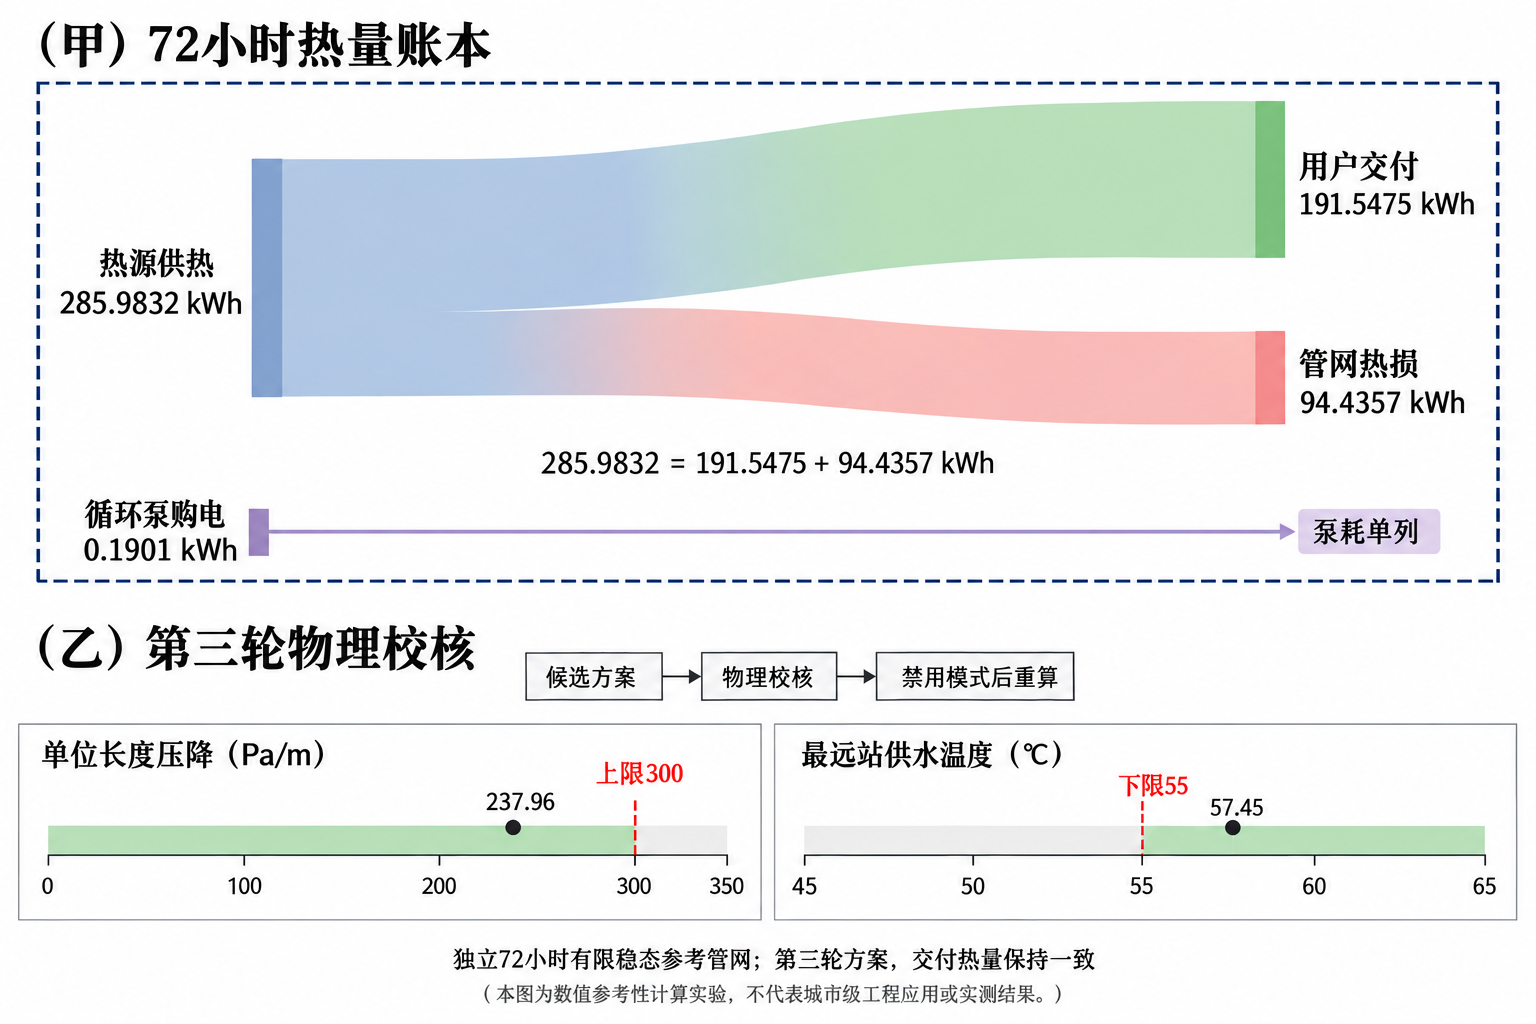
\includegraphics[width=0.96\linewidth]{results-a3/energy_balance_a3.png}
\caption[72小时参考管网的热量账本与物理校核]{72小时参考管网的热量账本与物理校核。循环泵购电单列；流带及点位示意分配关系与阈值比较，精确值以标注为准。仅在校核失败时禁用模式后重算；第三轮通过两项阈值后结束，前两轮与费用变化保留于本节表格。}
\label{fig:r8p-energy-a3}
\end{figure}

每轮时限60秒、目标gap0，均保留原求解状态、gap0与物理检查的分离记录。达标轮的历史结果属性因原浮点下界略大于可行值而保守记为缺证据，不升级为严格全局证明；物理可行审计仍通过。该有限稳态检查未覆盖冷启动、运输时滞、共泵水力平衡、RC脉冲舒适度、投资或动态故障认证。

\noindent\textbf{记录入口：}\path{docs/implementation_20261002_followup/parallel_stage_03/network/run_02/}，含\path{protocol.json}、\path{config.yaml}、\path{hourly.csv}、\path{comparison.json}、\path{manifest.json}与\path{failures.json}；\path{results/soft_off/history.json}和\path{results/soft_on/history.json}保留全部两轮拒绝及达标轮，不只展示最终通过点。

\subsection*{5.5\quad E08：四楼固定投资连续状态检查}
该组是武汉已登记合成参数数学场景，以相同规划方案冻结投资后复算四个独立建筑状态，并非四楼现场测温验证。服务年为北京时间2023年7月1日至2024年7月1日，共8784小时；声明冬季为2023年11月15日至2024年3月16日，共2928小时，均含起点、不含终点。

\begin{table}[H]
\centering
\caption{四楼两组连续窗口全部结果与运行层属性}
\begin{tabularx}{\linewidth}{@{}YrrL{0.22\linewidth}@{}}
\toprule
项目 & 服务年 & 声明冬季 & 解释\\\midrule
小时 & 8784 & 2928 & 单个连续窗口\\
交付热量/kWh & 958337.82 & 930728.48 & 四楼合计\\
交付冷量/kWh & 1327093.47 & 711.22 & 冷服务另核\\
现金运行费/元 & 285195.84 & 122974.20 & 仅对应本窗口\\
求解gap/\% & 0.1344 & 0.4755 & 请求容差0.5\%\\
求解时间/s & 133.07 & 48.21 & 总墙钟另留存\\
最大RC残差/$^\circ$C & $1.10\times10^{-13}$ & $6.75\times10^{-14}$ & 独立逐楼复算\\
舒适/初末违约 & 0/0 & 0/0 & 登记边界内\\
\bottomrule
\end{tabularx}
\end{table}

服务年现金总成本按纠正账本为586978.7050元，其中年化资本301782.8654元已包含一次；不能再次叠加资本。声明冬季122974.2004元只作同期运行费，不折成年费用、利润或回收期。两组运行请求时限分别1800/900秒，均在0.5\%登记容差内报告Optimal且状态检查通过，含固定投资标记、数值审计及新增投资零检查；仍不能说明投资计划联合最优。来源等级记录保留低等级设备参数，RC检查范围不替代热源、网络或真实建筑校准。

\noindent\textbf{记录入口：}原工程\path{outputs/competition_20261001/C4/optimized_annual_01/}与\path{outputs/competition_20261001/C4/optimized_season_03/}的\path{run_record.json}、\path{summary.json}、\path{independent_rc_audit.json}、\path{c6_building_audit.json}、\path{corrected_cost.json}及逐时轨迹。既有R8L源包\path{evidence/C4/ARCHIVE_INDEX.json}登记原路径、原SHA与无损gzip副本；本轮核对压缩身份及解压原身份，不修改其历史来源审核状态。

\subsection*{5.6\quad E09：三城27条固定策略的全部六方法}
该组为已见三城的开发确认。每城2880小时、九策略、同八个真实代表日；六方法均先于真实策略电费/能耗完成校准。三城27条完整轨迹共77760小时，不声称减少仿真量。九策略编号0--8依次为零预热、全谷段1/3~$^\circ$C、05时末端1/3~$^\circ$C、13时末端1/3~$^\circ$C、双末端1/3~$^\circ$C；跨日状态继承、自然漂移上限27~$^\circ$C、最后一小时恢复20~$^\circ$C并计冷热能量。

预算均以各城同一完整季零预热电量为基线，倍率1、1.02、1.05、1.10；固定碳因子使能量/碳帽冗余。按估计费用在估计帽内选策略，费用并列容差$10^{-8}$元，再按最小策略编号；实际帽与服务另核，无估计可行策略不回退。遗憾只对实际可行选择计算，超帽/无选择留空；oracle只在相同九策略库内，不是全局调度最优。

\begin{table}[H]
\centering
\caption{六方法完整27策略估计与12次选择分母；误差列为\%}
\begin{tabularx}{\linewidth}{@{}Yrrrrr@{}}
\toprule
方法简名 & \shortstack{电费\\MAPE} & \shortstack{能量\\MAPE} & \shortstack{最大能量\\APE} & 合格/12 & 超帽/无选\\\midrule
频数 & 0.556911 & 0.267761 & 0.718644 & 9 & 2/1\\
软能量 & 0.448316 & 0.044228 & 0.291601 & 11 & 0/1\\
硬$W_1$ & 0.140535 & 0.057807 & 0.315063 & 12 & 0/0\\
硬最小$L_1$ & 0.460634 & 0.043351 & 0.289511 & 12 & 0/0\\
价/时窗配对$L_1$ & 0.485844 & 0.050416 & 0.289022 & 12 & 0/0\\
硬$W_1$加候选$L_1$上限 & 0.329306 & 0.045621 & 0.290410 & 12 & 0/0\\
\bottomrule
\end{tabularx}
\end{table}

\begin{table}[H]
\centering
\caption{电费MAPE的逐城分解，单位为\%}
\begin{tabularx}{\linewidth}{@{}Yrrr@{}}
\toprule
方法 & 乌鲁木齐 & 固原 & 武汉\\\midrule
频数 & 0.772160 & 0.094224 & 0.804347\\
软能量 & 0.698834 & 0.288920 & 0.357193\\
硬$W_1$ & 0.018529 & 0.341666 & 0.061409\\
硬最小$L_1$ & 0.696076 & 0.300437 & 0.385390\\
价/时窗配对$L_1$ & 0.523837 & 0.300437 & 0.633258\\
硬$W_1$加候选$L_1$上限 & 0.075426 & 0.300437 & 0.612056\\
\bottomrule
\end{tabularx}
\end{table}

\begin{table}[H]
\centering
\caption{全部城市与预算的选择；四种硬方法逐例同选，故合并显示}
\begin{tabularx}{\linewidth}{@{}Yrrrr@{}}
\toprule
城市/帽倍率 & 频数 & 软能量 & 四种硬方法 & 库内oracle\\\midrule
乌鲁木齐/1.00 & 无选 & 无选 & 0 & 0\\
乌鲁木齐/1.02 & 8 & 8 & 8 & 8\\
乌鲁木齐/1.05 & 8 & 8 & 8 & 8\\
乌鲁木齐/1.10 & 8 & 8 & 8 & 8\\
固原/1.00 & 3超帽 & 0 & 0 & 0\\
固原/1.02 & 8 & 8 & 8 & 8\\
固原/1.05 & 8 & 8 & 8 & 8\\
固原/1.10 & 8 & 8 & 8 & 8\\
武汉/1.00 & 3超帽 & 0 & 0 & 0\\
武汉/1.02 & 4 & 4 & 4 & 4\\
武汉/1.05 & 8 & 8 & 8 & 8\\
武汉/1.10 & 8 & 8 & 8 & 8\\
\bottomrule
\end{tabularx}
\end{table}

频数的两次超帽分别为12.5160、12.6716~kWh，原遗憾留空；不能把九次有效遗憾为0改说成12次全部成功。四种硬法均12次实际合格且选到库内oracle，遗憾均0，故没有新候选优于硬$W_1$选策的证据。冻结规则按合格数、遗憾、最大能量APE等排序，仍登记价/时窗配对$L_1$；其最大能量APE比最小$L_1$仅低0.000489个百分点，电费MAPE却约为硬$W_1$的3.46倍。固原硬$W_1$电费MAPE还高于频数，逐城结果不能被总平均掩盖。代理热量守恒不等于策略电量/电费精确，价格矩和05/13时窗约束共同改变，不能据联合候选单独证明价格矩因果贡献。

独立42225项记录检查及全部27轨迹RC/服务/初末/容量/互斥检查通过；首次审计因两处约$9.09\times10^{-13}$元的并列翻位失败，原记录保留，补充精度审计未改权重、协议或阈值。运行29.135秒、共同准备0.648秒分别记录，全真值计算计入成本；不把不同方法的依赖成本或仿真成本省略后声称提速。

\noindent\textbf{记录入口：}\path{docs/implementation_20261002_followup/parallel_stage_03/algorithm/}，含\path{confirmation_run_01/protocol.json}、\path{manifest.json}、\path{truth.json}、\path{selections.json}、\path{predictions.json}、\path{failures.json}、完整轨迹与逐日表；\path{analysis_01/method_summary.csv}、\path{budget_selections.csv}及\path{policy_predictions.csv}保存完整分母，\path{claims_reviewed.txt}、\path{interpretation.json}和\path{verification_02/audit.json}限定结论。原三城天气已用于开发，模型为共同公开原型及方法学电价；无新留出泛化、实际投资改善或在线预测主张。

\subsection*{5.7\quad 身份、复算范围与交付说明}
本轮R8P对既有证据索引和新增引用文件计算SHA-256，并从保存的JSON/CSV重新汇总六楼中位数、采用分母、热容四格差值和27策略误差，核对正文及附录的舍入数值；不重新运行求解器、不累计历史测试，也不将此前通过记录改成本轮新实验。完整小时调度留在各原证据目录，附录展示所有实验单元与拒绝/超帽/无选分母，不打印数万小时流水。

正文保留\path{minor:supplement}标题锚点，表\ref{tab:r8p-comparisons}仅列E01/E03；原\path{tab:minor-evidence}移至本附录总表，仍含管网反馈和四楼连续状态，因而主文工程反馈、创新及评分页的原交叉引用没有变成另一组实验。历史结果的原始来源、模型版本、投资范围、求解容差和适用限制随记录保留。

% !TeX root = ../main.tex
\clearpage
\section*{附录6\quad 推荐采纳书}
\phantomsection
\addcontentsline{toc}{section}{附录6：推荐采纳书（待推荐单位填写签章）}
\begingroup
\fontsize{10.5pt}{13pt}\selectfont\setstretch{1.0}\setlength{\parskip}{5pt}
\begin{center}\textbf{供推荐单位审核填写}\end{center}
\noindent 成果名称：暖城向新·热力不息——城镇供热源荷匹配与规划寻优模型\par
\noindent 送审版本：原结构附录详编版 R8P（2026年10月4日）\par
\noindent 完成单位及负责人：\hrulefill\par
\noindent 推荐／采纳单位：\hrulefill\par
\noindent 联系人及联系电话：\hrulefill\par

\noindent\textbf{一、审核及应用情况}\par
\noindent 审阅材料、交流或试用时间：\hrulefill\par
\noindent 对应项目、应用对象与范围：\hrulefill\par
\noindent\rule{\linewidth}{0.3pt}\par
\noindent 应用状态（由单位勾选）：$\square$ 已审阅，建议进一步验证\quad $\square$ 拟开展试用\par
\noindent\hspace{2em}$\square$ 已试用\quad $\square$ 已采纳（请填写时间及证明材料编号）\par
\noindent 证明材料或可核验记录：\hrulefill\par

\noindent\textbf{二、推荐／采纳意见}\par
\noindent 请结合实际审核或应用情况，填写模型适用性、技术特点、应用效果及推荐范围。\par
\vspace{5pt}
\noindent\rule{\linewidth}{0.3pt}\par\vspace{5pt}
\noindent\rule{\linewidth}{0.3pt}\par\vspace{5pt}
\noindent\rule{\linewidth}{0.3pt}\par\vspace{5pt}
\noindent\rule{\linewidth}{0.3pt}\par
\vspace{8pt}
\noindent 单位负责人／授权代表签字：\hrulefill\par
\noindent 单位盖章：\hfill 年\hspace{1.5em}月\hspace{1.5em}日\par
\vspace{5pt}
{\wuhao 本页为待填写表单。推荐、试用与采纳状态以单位据实填写及签章的内容为准。}

\endgroup

\end{document}
